% 高一160_奉贤中学_期中.tex
%   —— 高一上数学"2026-2027 年奉贤中学高一上期中"（试卷版/答案版/紧凑版）
% 试卷版：xelatex 高一160_奉贤中学_期中.tex
% 答案版：xelatex "\def\isanswer{1}% 高一160_奉贤中学_期中.tex
%   —— 高一上数学"2026-2027 年奉贤中学高一上期中"（试卷版/答案版/紧凑版）
% 试卷版：xelatex 高一160_奉贤中学_期中.tex
% 答案版：xelatex "\def\isanswer{1}% 高一160_奉贤中学_期中.tex
%   —— 高一上数学"2026-2027 年奉贤中学高一上期中"（试卷版/答案版/紧凑版）
% 试卷版：xelatex 高一160_奉贤中学_期中.tex
% 答案版：xelatex "\def\isanswer{1}% 高一160_奉贤中学_期中.tex
%   —— 高一上数学"2026-2027 年奉贤中学高一上期中"（试卷版/答案版/紧凑版）
% 试卷版：xelatex 高一160_奉贤中学_期中.tex
% 答案版：xelatex "\def\isanswer{1}\input{高一160_奉贤中学_期中.tex}"
% 紧凑版：xelatex "\def\iscompact{1}\input{高一160_奉贤中学_期中.tex}"
%
% ① 原始材料：微信公众号"魔都数学加油站"文章，连载"27学年高一160"，原卷卷面标题
% "2026-2027 年奉贤中学高一上期中"（卷面未印副标题、未印连载号）。
% 正文为 10 张 PNG 页（01/04/10 为 2560×3620，02/03/05/06/07/08/09 为
% 4762×6735，同一篇各页分辨率混排，逐页按各自分辨率裁图核对）。
% 体例：讲评版——填空 3—12（10 题）、选择 13—16（4 题）、解答 17—21（5 题），
% 共 19 题，自第 3 题起编（1、2 未印在本篇）；19 题逐题印【解析】，无只印【答案】
% 的题；四道选择题答案在解析末句"故选 $B$/$B$/$D$/$C$"，题干括号
% \mbox{（\quad）} 留空、不另提 \ans{}。题目、答案、解析均据原图转录；卷面粉红色
% 水印"魔都数学加油站"及公众号页脚未录入。
% 全卷插图清单（逐页通读 10 页确认）：2 幅，均为题目配图、三版都出——
%   · Q4 韦恩图（01 页右侧：矩形全集 U、两圆 A/B、阴影部分 B∩上划线 A、
%     标注 U/A/B），裁 figures/gao160_q4.png；
%   · Q16 等腰直角三角形 ABC 图（05 页右下：C 顶点、A/O/D/B 共线底边、
%     CO 与 CD 两条线段），裁 figures/gao160_q16.png；
%   两图均取原卷截图 3—4× LANCZOS 放大、去粉色水印、转灰度、autocontrast；
%   Q4 图左侧题干残字"示"、Q16 图左侧题干残字均已裁白。
%   Q19 有一张 3 行数据表（t／届数／运动员人数（y 人），t=0..4），按全稿
%   成例（高一130）用 tabular 重排，不做成 png；其余各页无题目配图、
%   无解析内配图、无其它表格、无"如图"处。
%
% 卷首标题：原卷印作"2026-2027 年奉贤中学高一上期中"，年份区间按全稿惯例排 en dash；
% 原卷卷面未印副标题，本稿按同期中卷知识模块口径补出"集合与常用逻辑用语、不等式、函数"。
%
% ② 与原卷的排版差异／照录项清单：
%   ① 原文从第 3 题起，本稿保留原题号；共 19 题三节，解答题 5 题到 21；
%      三节各自一个 enumerate + \setcounter{enumi}{2}/{12}/{16}（不贯穿），
%      用 \examtitlest[3] 起手；
%   ② 混合体例说明：19 题全印【解析】、用 \solbegin…\solend，无只印【答案】
%      或答案印括号内的题；四道选择题答案在解析末句"故选 $B$/$B$/$D$/$C$"
%      （逐个放大复核）、括号 \mbox{（\quad）} 留空、不另提 \ans{}；答案版
%      【答案】/【解析】标记数 = 19 = 全卷题数（0 个 \ans ＋ 19 个 \solbegin）；
%   ③ 原卷卷面未印副标题，本稿按知识模块口径补出；
%   ④ 原卷填空横线按全稿惯例排 \blankline[4.4em]；选择题括号排 \mbox{（\quad）}、
%      四道选择题的选项段前按惯例各加 \keepwithprev；解答题不留作答区、不加
%      \anspace（原卷为讲评版，109—113 起全稿不用 \anspace）；
%   ⑤ 数集归一：Q4"$U=\Z$"、Q9"$a\in\R$，$b\in\R$"、Q11"$n\in\Z$"、
%      Q15"$s\in\R$"、Q21"$n\in\N$""$a_i\in\N$"原卷印正体粗体 Z/R/N，
%      按全稿惯例归一 \Z／\R／\N；集合描述竖线排 \mid（Q3、Q4、Q12、
%      Q18、Q21）；空集 \varnothing（Q18 解析 (2)）；补集照原卷上划线排
%      \overline{A}（Q4 解析、Q18 (1) 题干与解析）；子集符号 Q18 两处
%      "$A\subseteq B$"印带下划线 ⊆、照录 \subseteq；
%   ⑥ 绝对值排 \lvert…\rvert（Q7、Q8 题干与解析、Q9 题干、Q16 解析、
%      Q18 题干与解析），Q16 解析的 \left\lvert…\right\rvert 与 \lvert…\rvert
%      均在同一 $…$ 组内配对平衡；
%   ⑦ 判别式两形混用逐处照录不统一（放大逐处确认）：Q3 解析
%      "$\triangle=1^2-4a\times\frac{1}{4}=0$"原卷印扁等边三角、照录
%      \triangle；Q17 解析 cases 块"$\Delta=(t+1)^2-4t^2=(1-t)(3t+1)>0$"
%      原卷印等腰偏高三角、照录 \Delta；Q16 题干几何符号"$\triangle ABC$"
%      按全稿几何三角形记号惯例归一 \triangle（参照 高一150／132 成例）；
%   ⑧ 不等号按全稿惯例排 \leqslant／\geqslant；中文弯引号照录：Q9 题干
%      "充分非必要""必要非充分""充要""既非充分又非必要"、Q14 题干
%      "存在 $x\in(1,+\infty)$，使得 $f(x)>0$"与解析"存在""对任意"、
%      Q21 题干与解析多处"和积平衡集"；注释里一律 ASCII 引号；
%   ⑨ 文本圈数字逐处照录：Q12 题干①②③、Q12 解析"故①正确""同②得"
%      "故②正确""③假设""故③错误""故真命题是①②"、Q19 题干①②与解析
%      "选模型①"，均为印刷圈数字（非 \textcircled、非数学模式）；
%   ⑩ 半角逗号在数学组之间是全稿惯例、非笔误，逐处照录（Q8"$2^t,2^{-t}$"、
%      Q9"$a=-1,b=-2$""$a=1,b=-1$"、Q11"$1\leqslant a<10,n\in\Z$"、
%      Q12"$s_1=\frac{1}{2},t_1=x_n$"、Q16 选项"$a>0,b>0$"与解析
%      "$CO=AO=\frac{a+b}{2},OD=...$"、Q18"$2<x\leqslant5,B=(2,5]$"
%      "$3<x<2a-3,A=(3,2a-3)$"、Q21"$n=2,3$"等）；行中全角逗号／顿号
%      照录（Q15 选项"$a>1$，且 $s>0$"、Q12 解析"$s$、$t$"、Q21 解析
%      "$a_1$、$a_2$"），顿号一律移出数学模式；
%   ⑪ "图像／图象"逐处照录：本卷 Q5"的图像恒过一个定点"、Q10"的图像经过点"、
%      Q13 题干两处"图像"与解析"对称图像对应的函数"均印"图像"（有亻）；
%      Q16 印"图形"（利用图形说明、该图形能说明），无"图象"用例；
%   ⑫ 复杂式照录别简化：Q3 $ax^2+x+\frac14=0$、Q5 $y=\log_a(5x-9)-4$、
%      Q6 $(1-2x)^{\frac34}>x^{\frac34}$ 与 $\left[0,\frac12\right]$、
%      Q8 $\frac{s+\sqrt{s^2-4}}{2}$、Q10 $y=\frac{2^x}{2^x+ax}$ 与
%      $\frac{2^p}{2^p+ap}=\frac56$、$\frac{2^q}{2^q+aq}=\frac16$、
%      Q11 $N=a\times10^n$ 与 $3^{2026}$、$2026\lg3\approx966.60$、
%      $966.64512<2026\lg3<966.66538$、Q12 $Y=\{(s,t)\mid s\in X,t\in X\}$
%      与 $\frac12 s+tx_n=0$、Q16 $\sqrt{\frac{a^2+b^2}{2}}$、
%      Q17 $x^2-(t+1)x+t^2=0$ 与 $\left(-\frac13,0\right)\cup(0,1)$、
%      Q18 $\frac{5-x}{x-2}\geqslant0$、Q19 $y=a\cdot b^t+c$ 与
%      $y=\log_a(t+b)+c$、$y=7\cdot2^t-3$、Q20 $f(x)=\log_a(a-a^x)$
%      与 $a^2-a-1\geqslant0$、$\left[\frac{1+\sqrt5}{2},+\infty\right)$、
%      Q21 $4+2\sqrt2$ 与 $(a_2-1)(a_3-1)=2$ 等；
%   ⑬ 子题标号 (1)(2)(3) 按全稿惯例排半角括号；行末／行中句点按全稿惯例
%      排 ASCII `.`（不是全角「．」）；cases 块整体算一个印刷行
%      （Q17 解析、Q19 解析 (1)）；
%   ⑭ 配图：Q4／Q16 题目配图（三版都出）放 \item 内题干之后 \begin{center}，
%      各用 \needvspace{8cm} 守卫把整块推走，**守卫放在 \item 之前**
%      （见 高一153 Q11/Q19 成例与切页审计 B 类坑）；
%   ⑮ 一条 \step = 原卷解析的一个印刷行；跨上下半页的重叠行只算一次
%      （Q4 解析、Q9 解析首行、Q11 解析首行、Q12 解析"若 $s=-1$…"一行、
%      Q18 解析"此时 $A\subseteq B=(2,5]$…"一行、Q20 (2) 题干、
%      Q21 解析"由 $1\leqslant a_2-1<a_3-1$…"一行）；原卷折行别合并；
%   ⑯ Q10 之后另有一整块【注】按语（03 页上半，5 个印刷行），是讲评版作者对
%      原卷数据自相矛盾的加注、不属于任何题的【解析】。本稿按 高一53
%      "注：…"成例放 Q10 的 \solend 之后、Q10 的 \fi 收尾之前：
%      **整块只保留 Q10 那一层外层 \ifanswer**（那个 \fi 就是 Q10 的收尾），
%      块内 \stepm{【注】}{首行} ＋ 4 条 \step 各自自带内层 \ifanswer…\fi
%      （\step／\stepm 宏内自带，源码里不手动再包一层 \ifanswer，
%      否则 题目溯源.py 的 strip_answers 非贪婪正则会错切）；
%      \stepm 第一参数直接用「【注】」作标签，与全稿 \ans 的【答案】、
%      \solbegin 的【解析】同性质，未加粗以外不另加任何样式；
%      5 行仅答案版出、不新增 \item、不影响溯源，头注 ③ 单列登记、
%      不计入 19 题逐题 \step 账；\stepm 把【注】排成加粗着色标签
%      （原卷为黑色加粗），此一处着色差异在此登记；
%   ⑰ 原卷用字照录：Q11"约翰·纳皮尔""莱布尼兹"（原卷作"兹"，非通行"茨"）、
%      "17 世纪的三大数学发明"；Q16"数学说明的方法""点 $D$ 为斜边 $AB$ 上
%      异于顶点的一个动点"；Q19"登上赛场""以此类推"；
%
% ③ 行数复核：一条 \step = 原卷解析的一个印刷行，cases 块作一个印刷行计。
%   逐题数（逐页核对定稿）：Q3：5；Q4：1；Q5：1；Q6：2；Q7：2；Q8：4；
%   Q9：4；Q10：3；Q11：6；Q12：19；Q13：1；Q14：2；Q15：3；Q16：3；
%   Q17：7；Q18：8；Q19：6；Q20：12；Q21：18。
%   合计 107 条 \step（19 题逐题印刷行账），与原卷逐题印刷行相等。
%   **本卷源码 \step 总数 = 19 题逐题合计 107 ＋ Q10 后独立【注】块 5 行
%   = 112 行**（其中 \step 111 条、\stepm 1 条；\stepm 与 4 条 \step 合为
%   【注】块 5 印刷行）。该 5 行不计入「逐题印刷行」账，也不是任何题的
%   【解析】，而是讲评版编者按语；主会话核验脚本按全文统计 \step 时总数会
%   较逐题账多 5，已与主会话对齐、属已知预期而非错误。
%   全卷 19 题均设 \solbegin…\solend，答案版【答案】/【解析】标记数
%   = 19 = 全卷题数。
%
% ④ 页码分布（供回原图复核）：
%   卷首标题＋"一、填空题"＋Q3 题干＋解析 5 行＋Q4 题干＋韦恩图＋解析
%   1 行＋Q5 题干首行在 01 页上半；Q4 解析（重叠）＋Q5 题干续＋解析 1 行＋
%   Q6 题干＋解析 2 行＋Q7 题干＋解析首行在 01 页下半；Q7 解析末行＋
%   Q8 题干＋解析 4 行＋Q9 题干＋解析首行在 02 页上半；Q9 解析（重叠首行）
%   ＋余 3 行＋Q10 题干＋解析 3 行在 02 页下半；【注】按语 5 行＋Q11 题干＋
%   解析首行在 03 页上半；Q11 解析（重叠首行）＋余 5 行＋Q12 题干＋①②
%   在 03 页下半；Q12 ③＋解析前 9 行在 04 页上半；Q12 解析（重叠 2 行）
%   ＋余 8 行在 04 页下半；Q12 解析末 2 行＋"二、选择题"＋Q13 题干＋选项＋
%   解析 1 行＋Q14 题干＋选项＋解析首行在 05 页上半；Q14 解析末行＋
%   Q15 题干＋选项＋解析 3 行＋Q16 题干＋三角形图在 05 页下半；
%   Q16 选项＋解析 3 行＋"三、解答题"＋Q17 题干＋两问在 06 页上半；
%   Q17 解析 7 行在 06 页下半；Q18 题干＋两问＋解析前 7 行＋Q19 题干首行
%   在 07 页上半；Q18 解析末行（重叠）＋Q19 题干＋表格＋两问在 07 页下半；
%   Q19 解析 6 行＋Q20 题干＋(1)(2) 在 08 页上半；Q20 (2)(3) 题干（重叠）
%   ＋解析 8 行在 08 页下半；Q20 解析末 4 行＋Q21 题干＋(1)(2) 在 09 页
%   上半；Q21 (3)＋解析前 7 行在 09 页下半；Q21 解析 (3) 余 10 行在 10 页
%   上半；Q21 末行（重叠）＋"检验 $1+2+3=1\times2\times3=6$，所求集合为
%   $\{1,2,3\}$."在 10 页下半（此后仅水印、无正文）。本稿按题连排，
%   不丢行、不并折行；全卷末题为第 21 题，无附加题节。
%
% ⑤ 存疑照录（放大原图确认，照录未改、正文对应处另有 % 注）：
%   1. Q10【注】按语：讲评版作者据 $a=\sqrt3$ 时 $2^q=\frac{\sqrt3}{5}q<q$
%      与 $2^n\geqslant n+1$ 推出点 $Q$ 不存在、"严格说本题无解"，并注明
%      "原卷数据疑似有误（同型常见题为 $P(p,\frac65)$、$Q(q,-\frac15)$、
%      $2^{p+q}=36pq$，得 $a=6$）"；本稿照录全块、未删未改（见 ② ⑯）。
%   2. Q12 解析 (3) 末段"若 $t=-1$，则 $\frac{1}{2}s=x_n\cdot(-1)$，
%      于是 $s=2x_n>x_n$，也矛盾，"中，等式右端与紧随的结论符号不自洽
%      （按题意应为 $\frac12 s=x_n$ 或 $-\frac12 s=x_n\cdot(-1)$），逐页
%      放大 04 页确认原卷即如此印、无漏看的负号，照录未改，建议主会话
%      回 04 页再放大复核一次；
%   3. Q19 解析 (1) 印"选模型①"（圈数字①，题干只有①②两种模型）；
%      OCR 误作"选模型四"，放大 08 页确认是①、照录①；
%   4. Q20 解析 (1)"即 $a^x<a^1$"末项原卷印 $a^1$（非 $a$），照录未化简；
%   5. Q11 题干"莱布尼兹"原卷作"兹"（非通行"茨"）、"约翰·纳皮尔"用
%      间隔号·，均照录未改；
%   6. Q9 题干"则 $p$ 是 $q$___条件"与解析"故 $p$ 是 $q$ 的充分非必要条件"
%      句式略异，均照录；
%   7. Q19 解析 (1) 用"前 3 组数据"、题干表格列到 $t=4$，照录未补。
%
\documentclass[a4paper,11pt]{article}
\usepackage{common}

\begin{document}

\examtitlest[3]{2026--2027 年奉贤中学高一上期中}{集合与常用逻辑用语、不等式、函数}

\bigsec{一、填空题}

\begin{enumerate}
\setcounter{enumi}{2}

% === Q3 === 解析 5 行；判别式印扁等边三角 \triangle
\item 若集合 $A=\{x\mid ax^2+x+\dfrac{1}{4}=0\}$ 有且仅有两个子集，则实数 $a=$\blankline[4.4em].

\ifanswer
\solbegin
\step{若集合 $A=\{x\mid ax^2+x+\dfrac{1}{4}=0\}$ 有且仅有两个子集，}
\step{所以方程 $ax^2+x+\dfrac{1}{4}=0$ 只有一个实数根，}
\step{当 $a=0$ 时，方程化为 $x+\dfrac{1}{4}=0$，解得 $x=-\dfrac{1}{4}$，符合题意，}
\step{当 $a\ne0$ 时，则 $\triangle=1^2-4a\times\dfrac{1}{4}=0$，解得 $a=1$，}% 判别式原卷印扁等边三角 \triangle，照录
\step{综上所述，实数 $a=0$ 或 1.}
\solend
\fi

% === Q4 === 题目配图（三版都出）；\needvspace 守卫放 \item 之前；补集上划线 \overline{A}；解析 1 行
\needvspace{8cm}
\item 设全集 $U=\Z$，集合 $A=\{x\mid -3<x<1\}$，$B=\{-1,0,1,2\}$，用列举法表示图中阴影部分为\blankline[4.4em].

\begin{center}
% Q4 韦恩图（全集 U、A/B 两圆、阴影 B∩上划线 A）取 01 页右侧，去粉色水印、去色、4× LANCZOS 放大；三版都出
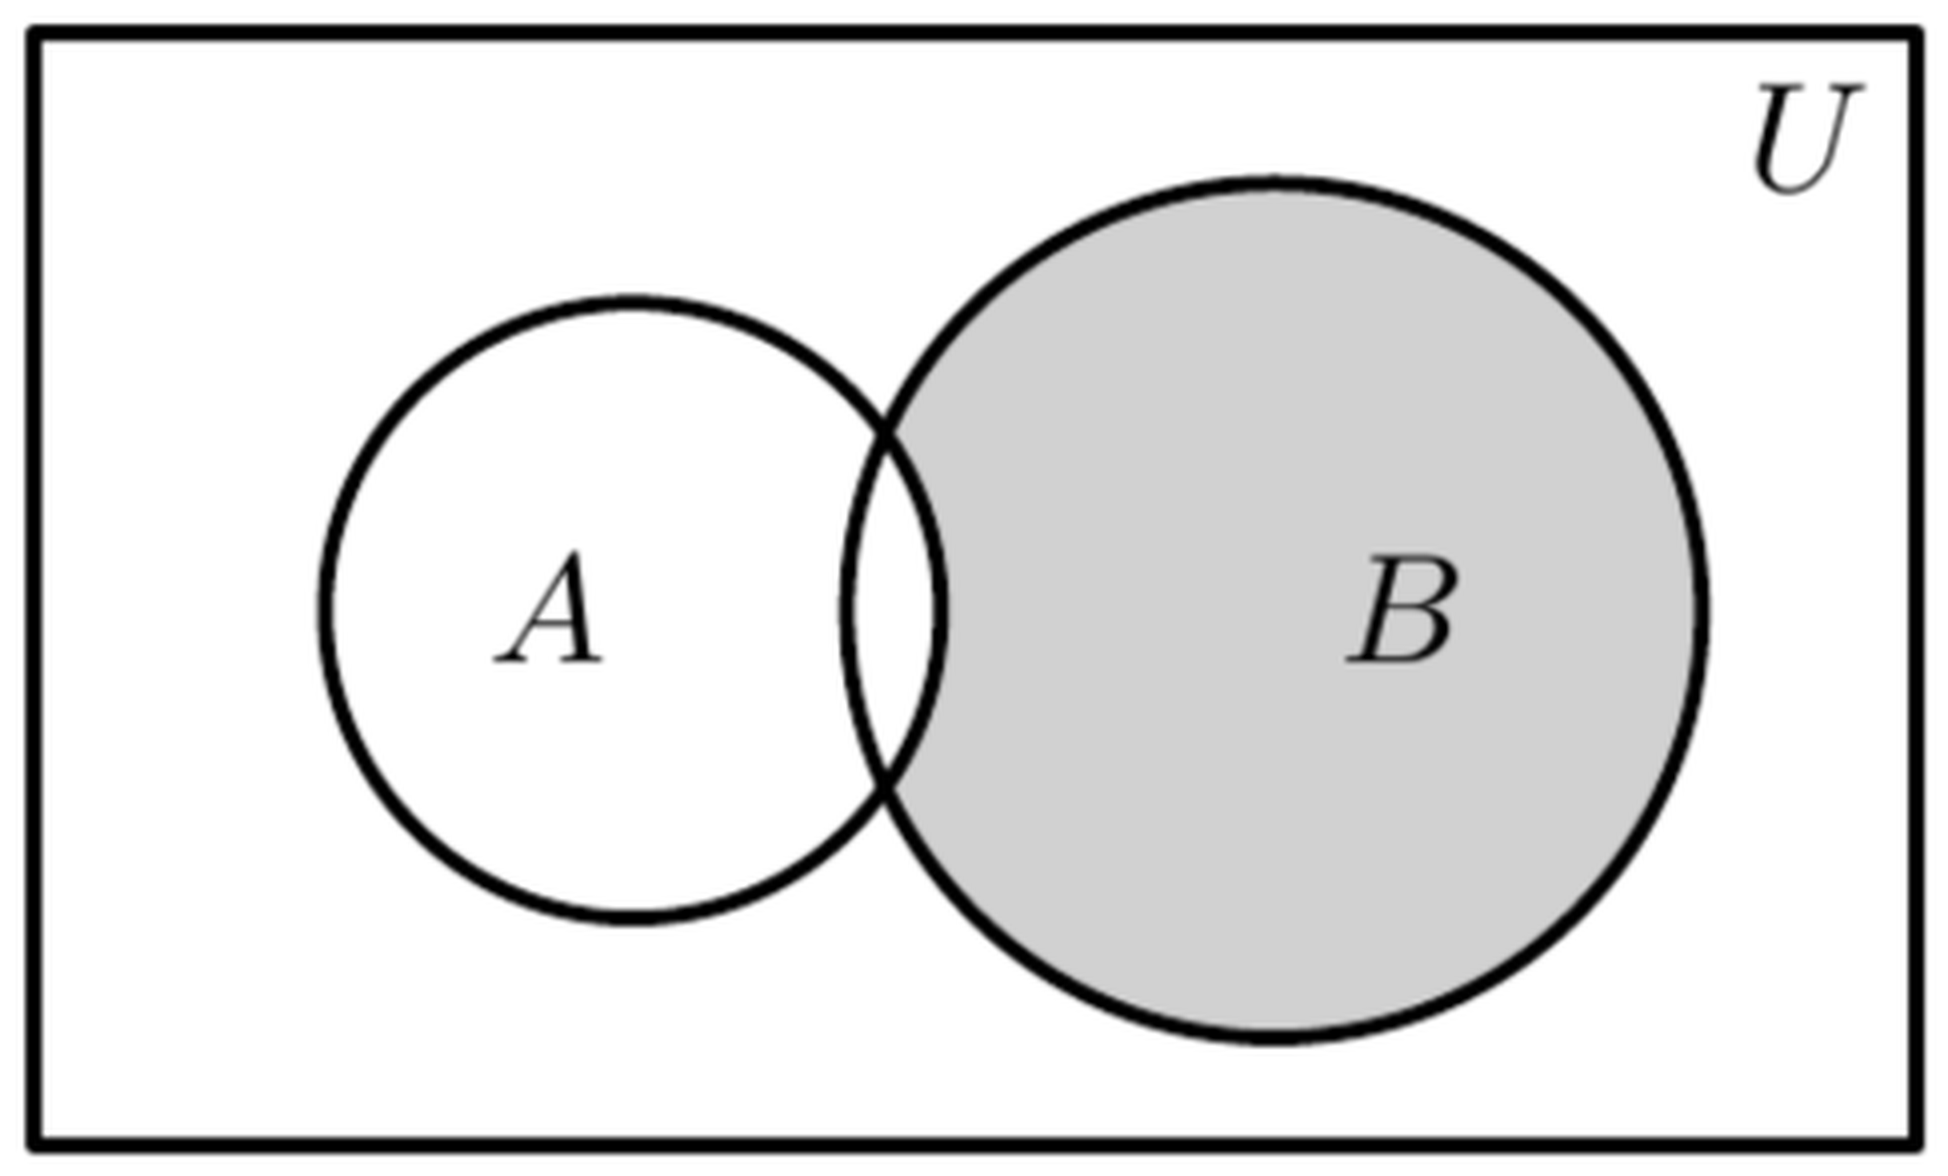
\includegraphics[width=0.38\textwidth]{figures/gao160_q4.png}
\end{center}

\ifanswer
\solbegin
\step{阴影部分表示 $B\cap\overline{A}=\{1,2\}$.}
\solend
\fi

% === Q5 === "图像"（有亻）照录；解析 1 行
\item 已知常数 $a>0$ 且 $a\ne1$，假设无论 $a$ 取何值，函数 $y=\log_a(5x-9)-4$ 的图像恒过一个定点，则这个定点的坐标为\blankline[4.4em].

\ifanswer
\solbegin
\step{$5x-9=1\Rightarrow x=2$，此时 $y=\log_a 1-4=-4$，定点为 $(2,-4)$.}
\solend
\fi

% === Q6 === 解析 2 行
\item 不等式 $(1-2x)^{\frac{3}{4}}>x^{\frac{3}{4}}$ 的解集为\blankline[4.4em].

\ifanswer
\solbegin
\step{定义域为 $\left[0,\dfrac{1}{2}\right]$，由幂函数的单调性，原不等式等价于 $1-2x>x$，}
\step{得 $0\leqslant x<\dfrac{1}{3}$，故解集为 $\left[0,\dfrac{1}{3}\right)$.}
\solend
\fi

% === Q7 === 绝对值 \lvert…\rvert；解析 2 行（跨 01—02 页）
\item 已知不等式 $\lvert x+3\rvert+\lvert x-2\rvert\geqslant 5$，当其等号成立时，$x$ 的取值范围是\blankline[4.4em].

\ifanswer
\solbegin
\step{$\lvert x+3\rvert+\lvert x-2\rvert=\lvert x+3\rvert+\lvert 2-x\rvert\geqslant\lvert(x+3)+(2-x)\rvert=5$，}
\step{等号成立当且仅当 $(x+3)(2-x)\geqslant0$，即 $x\in[-3,2]$.}
\solend
\fi

% === Q8 === 解析 4 行
\item 已知函数 $f(x)=\lvert\log_2 x\rvert$，若方程 $f(x)-t=0$ 有两个不同的实数根 $x_1,x_2$，则 $x_1+x_2$ 的取值范围是\blankline[4.4em].

\ifanswer
\solbegin
\step{方程有两个不同实根，必有 $t>0$，两根为 $2^t,2^{-t}$，}
\step{所以 $x_1+x_2=2^t+2^{-t}>2$（等号仅在 $t=0$ 时成立）.}
\step{任取 $s>2$，令 $a=\dfrac{s+\sqrt{s^2-4}}{2}>1$，取 $t=\log_2 a>0$，则 $x_1+x_2=a+\dfrac{1}{a}=s$，}
\step{所以取值范围为 $(2,+\infty)$.}
\solend
\fi

% === Q9 === 中文弯引号、\R、绝对值 \lvert…\rvert；解析 4 行
\item 已知 $a\in\R$，$b\in\R$，$p:\dfrac{1}{\lvert a\rvert}>\dfrac{1}{\lvert b\rvert}$，$q:\dfrac{1}{a}>\dfrac{1}{b}$，则 $p$ 是 $q$\blankline[4.4em]条件（用“充分非必要”、“必要非充分”、“充要”或“既非充分又非必要”填空）.

\ifanswer
\solbegin
\step{由 $p$、$q$ 中的分式有意义，$a\ne0$ 且 $b\ne0$.}
\step{当 $a=-1,b=-2$ 时，$p$ 成立而 $q$ 不成立，故 $p$ 不是 $q$ 的充分条件.}
\step{当 $a=1,b=-1$ 时，$q$ 成立而 $p$ 不成立，故 $p$ 不是 $q$ 的必要条件.}
\step{故 $p$ 是 $q$ 的充分非必要条件.}
\solend
\fi

% === Q10 === 解析 3 行；其后独立【注】按语 5 行（见头注 ② ⑯、⑤ 1）
\item 已知常数 $a>0$，函数 $y=\dfrac{2^x}{2^x+ax}$ 的图像经过点 $P\left(p,\dfrac{5}{6}\right)$、$Q\left(q,\dfrac{1}{6}\right)$，若 $2^{p+q}=3pq$，则 $a=$\blankline[4.4em].

\ifanswer
\solbegin
\step{由 $\dfrac{2^p}{2^p+ap}=\dfrac{5}{6}$ 得 $2^p=5ap$；由 $\dfrac{2^q}{2^q+aq}=\dfrac{1}{6}$ 得 $2^q=\dfrac{aq}{5}$.}
\step{$2^p>0$，$2^q>0$，$a>0$，得 $p>0$，$q>0$.}
\step{两式相乘得 $2^{p+q}=a^2pq$，又 $2^{p+q}=3pq$ 且 $pq\ne0$，故 $a^2=3$，$a=\sqrt{3}$.}
\solend
% 【注】按语（讲评版编者按，5 个印刷行，仅答案版出，不属于任何题的【解析】）
\stepm{【注】}{按原卷数据严格推敲，点 $Q$ 其实不存在：$a=\sqrt{3}$ 时 $2^q=\dfrac{\sqrt{3}}{5}q<q$；而当 $q>0$}
\step{时，取非负整数 $n$ 使 $n\leqslant q<n+1$，由 $2^{k+1}=2^k+2^k\geqslant2^k+1$ 逐次推得 $2^n\geqslant n+1$，于是}
\step{$2^q\geqslant2^n\geqslant n+1>q$，矛盾. 所以题设条件互相矛盾，严格说本题无解；$\sqrt{3}$ 是由题给关}
\step{系直接推出的值，按命题意图作为答案. 原卷数据疑似有误（同型常见题为 $P\left(p,\dfrac{6}{5}\right)$、}
\step{$Q\left(q,-\dfrac{1}{5}\right)$、$2^{p+q}=36pq$，得 $a=6$）.}% 见头注 ⑤ 1，照录未改
\fi

% === Q11 === 纳皮尔对数材料题；\Z、大数；解析 6 行
\item 17 世纪初，约翰·纳皮尔为了简化计算而发明了对数. 对数的发明是数学史上的重大事件，恩格斯曾经把笛卡尔的坐标系、纳皮尔的对数、牛顿和莱布尼兹的微积分共同称为 17 世纪的三大数学发明. 我们知道，任何一个正实数 $N$ 可以表示成 $N=a\times10^n$ ($1\leqslant a<10,n\in\Z$) 的形式，这便是科学记数法，若两边取常用对数，有 $\lg N=n+\lg a$，则可以估计 $3^{2026}$ 的最高位上的数值为\blankline[4.4em].

\ifanswer
\solbegin
\step{设 $3^{2026}=a\times10^n$ ($1\leqslant a<10,n\in\Z$)，则 $2026\lg 3=n+\lg a$.}
\step{用 $\lg 3\approx 0.4771$ 粗估，得 $2026\lg 3\approx 966.60$.}
\step{为核验误差，用 $0.47712<\lg 3<0.47713$，}
\step{得 $966.64512<2026\lg 3<966.66538$，因此 $n=966$.}
\step{于是 $\lg 4\approx 0.60206<0.64512<\lg a<0.66538<\lg 5\approx 0.69897$，}
\step{所以 $4<a<5$，最高位为 4，估算误差不影响结论.}
\solend
\fi

% === Q12 === 自定义"性质 P"；文本圈数字①②③；解析 19 行（跨 03—05 页）
\item 对于数集 $X=\{-1,x_1,x_2,x_3,\cdots,x_n\}$，其中 $0<x_1<x_2<x_3<\cdots<x_n$，$n\geqslant2$，定义点集 $Y=\{(s,t)\mid s\in X,t\in X\}$，若对于任意 $(s_1,t_1)\in Y$，存在 $(s_2,t_2)\in Y$，使得 $s_1s_2+t_1t_2=0$，则称集合 $X$ 具有性质 $P$. 则下列命题中为真命题的是\blankline[4.4em].

① $X=\{-1,1,2\}$ 具有性质 $P$；②若集合 $X$ 具有性质 $P$，则 $1\in X$；

③集合 $X$ 具有性质 $P$，若 $x_1=\dfrac{1}{2}$，则 $x_n=2$.

\ifanswer
\solbegin
\step{因为 $X=\{-1,1,2\}$，}
\step{所以 $Y=\{(-1,-1),(1,1),(2,2),(-1,1),(-1,2),(1,-1),(1,2),(2,-1),(2,1)\}$，}
\step{由集合 $X$ 具有性质 $P$ 的定义，对于任意 $(s,t)\in Y$，}
\step{若 $s>0$，$t>0$，则 $s=t$ 或 $(s,t)=(1,2)$ 或 $(s,t)=(2,1)$，}
\step{若 $s=t$，取 $s_2=-1$，$t_2=-1$，则 $ss_2+tt_2=0$；}
\step{若 $(s,t)=(1,2)$，取 $s_2=2$，$t_2=-1$，则 $ss_2+tt_2=0$；}
\step{若 $(s,t)=(2,1)$，取 $s_2=-1$，$t_2=2$，则 $ss_2+tt_2=0$；}
\step{若 $s$、$t$ 有一个为负数，则 $s=-1$ 或 $t=-1$，}
\step{若 $s=-1$，则取 $s_2=t$，$t_2=1$，则 $ss_2+tt_2=0$；}
\step{若 $t=-1$，则取 $s_2=1$，$t_2=s$，则 $ss_2+tt_2=0$；故①正确；}
\step{对于任意 $(s_1,t_1)\in Y$，存在 $(s_2,t_2)\in Y$，使得 $s_1s_2+t_1t_2=0$，}
\step{取 $(x_1,x_1)\in Y$，存在 $(x_p,x_q)$ 使得 $x_1x_p+x_1x_q=0$，所以 $x_p+x_q=0$，}
\step{不妨设 $x_p=1$，$x_q=-1$，所以若集合 $X$ 具有性质 $P$，则 $1\in X$，故②正确；}
\step{③假设 $x_n>1$，令 $s_1=\dfrac{1}{2},t_1=x_n$，则存在 $s$、$t\in X$ 使得 $\dfrac{1}{2}s+tx_n=0$，}
\step{同②得 $s$、$t$ 中必有一个数为 $-1$，}
\step{若 $s=-1$，则 $tx_n=\dfrac{1}{2}$，于是 $t=\dfrac{1}{2x_n}<\dfrac{1}{2}=x_1$，矛盾，}
\step{若 $t=-1$，则 $\dfrac{1}{2}s=x_n\cdot(-1)$，于是 $s=2x_n>x_n$，也矛盾，}% 原卷如此（与结论符号不自洽），照录未改，见头注 ⑤ 2
\step{所以 $x_n\leqslant1$，又由②得 $1\in X$，所以 $x_n\geqslant1$，所以 $x_n=1$，故③错误，}
\step{故真命题是①②.}
\solend
\fi

\end{enumerate}

% 答案版里填空解析把页排满，节标题会落到页末、与第 13 题分家（切页审计 B 类）；
% 守卫放 \bigsec 之前，连节标题一起量页高（高一157 成例）
\needvspace{7cm}
\bigsec{二、选择题}

\begin{enumerate}
\setcounter{enumi}{12}

% === Q13 === "图像"照录；解析 1 行，故选 $B$
\item 下列函数中，图像与函数 $y=3^x$ 图像关于 $y$ 轴对称的是\mbox{（\quad）}

\keepwithprev
A. $y=x^3$\qquad B. $y=\left(\dfrac{1}{3}\right)^x$\qquad C. $y=-3^x$\qquad D. $y=\log_3 x$

\ifanswer
\solbegin
\step{将 $x$ 换为 $-x$，得对称图像对应的函数为 $y=3^{-x}=\left(\dfrac{1}{3}\right)^x$，故选 $B$.}
\solend
\fi

% === Q14 === 中文弯引号；解析 2 行（跨 05 页上下），故选 $B$
\item 命题“存在 $x\in(1,+\infty)$，使得 $f(x)>0$”的否定形式为\mbox{（\quad）}

\keepwithprev
A. 不存在 $x\in(-\infty,1]$，使得 $f(x)>0$\qquad B. 对任意 $x\in(1,+\infty)$，有 $f(x)\leqslant0$

C. 对任意 $x\in(-\infty,1]$，有 $f(x)\leqslant0$\qquad D. 存在 $x\in(1,+\infty)$，使得 $f(x)\leqslant0$

\ifanswer
\solbegin
\step{将“存在”改为“对任意”，$x$ 的范围不变，并将 $f(x)>0$ 否定为 $f(x)\leqslant0$，}
\step{故选 $B$.}
\solend
\fi

% === Q15 === \R；四选项两行；解析 3 行，故选 $D$
\item 设 $a>0$，$s\in\R$. 下列各项中，能推出 $a^s>a$ 的一项是\mbox{（\quad）}

\keepwithprev
A. $a>1$，且 $s>0$\qquad B. $a>1$，且 $s<0$

C. $0<a<1$，且 $s>0$\qquad D. $0<a<1$，且 $s<0$

\ifanswer
\solbegin
\step{当 $a>1$ 时，$a^s>a\Leftrightarrow s>1$，A、B 均不能保证.}
\step{当 $0<a<1$ 时，$a^s>a\Leftrightarrow s<1$，C 不能保证，D 中 $s<0<1$，满足要求；}
\step{故选 $D$.}
\solend
\fi

% === Q16 === 题目配图（三版都出）；几何符号 \triangle ABC；解析 3 行，故选 $C$
\needvspace{8cm}
\item 数学说明的方法多种多样，其中利用图形说明就是一种重要方法. 如图所示，在等腰直角三角形 $\triangle ABC$ 中，点 $O$ 为斜边 $AB$ 的中点，点 $D$ 为斜边 $AB$ 上异于顶点的一个动点，设 $AD=a$，$BD=b$，则可用该图形能说明的不等式为\mbox{（\quad）}

\begin{center}
% Q16 等腰直角三角形 ABC 图（C/A/O/D/B 标注）取 05 页右下，去粉色水印、去色、3× LANCZOS 放大；三版都出
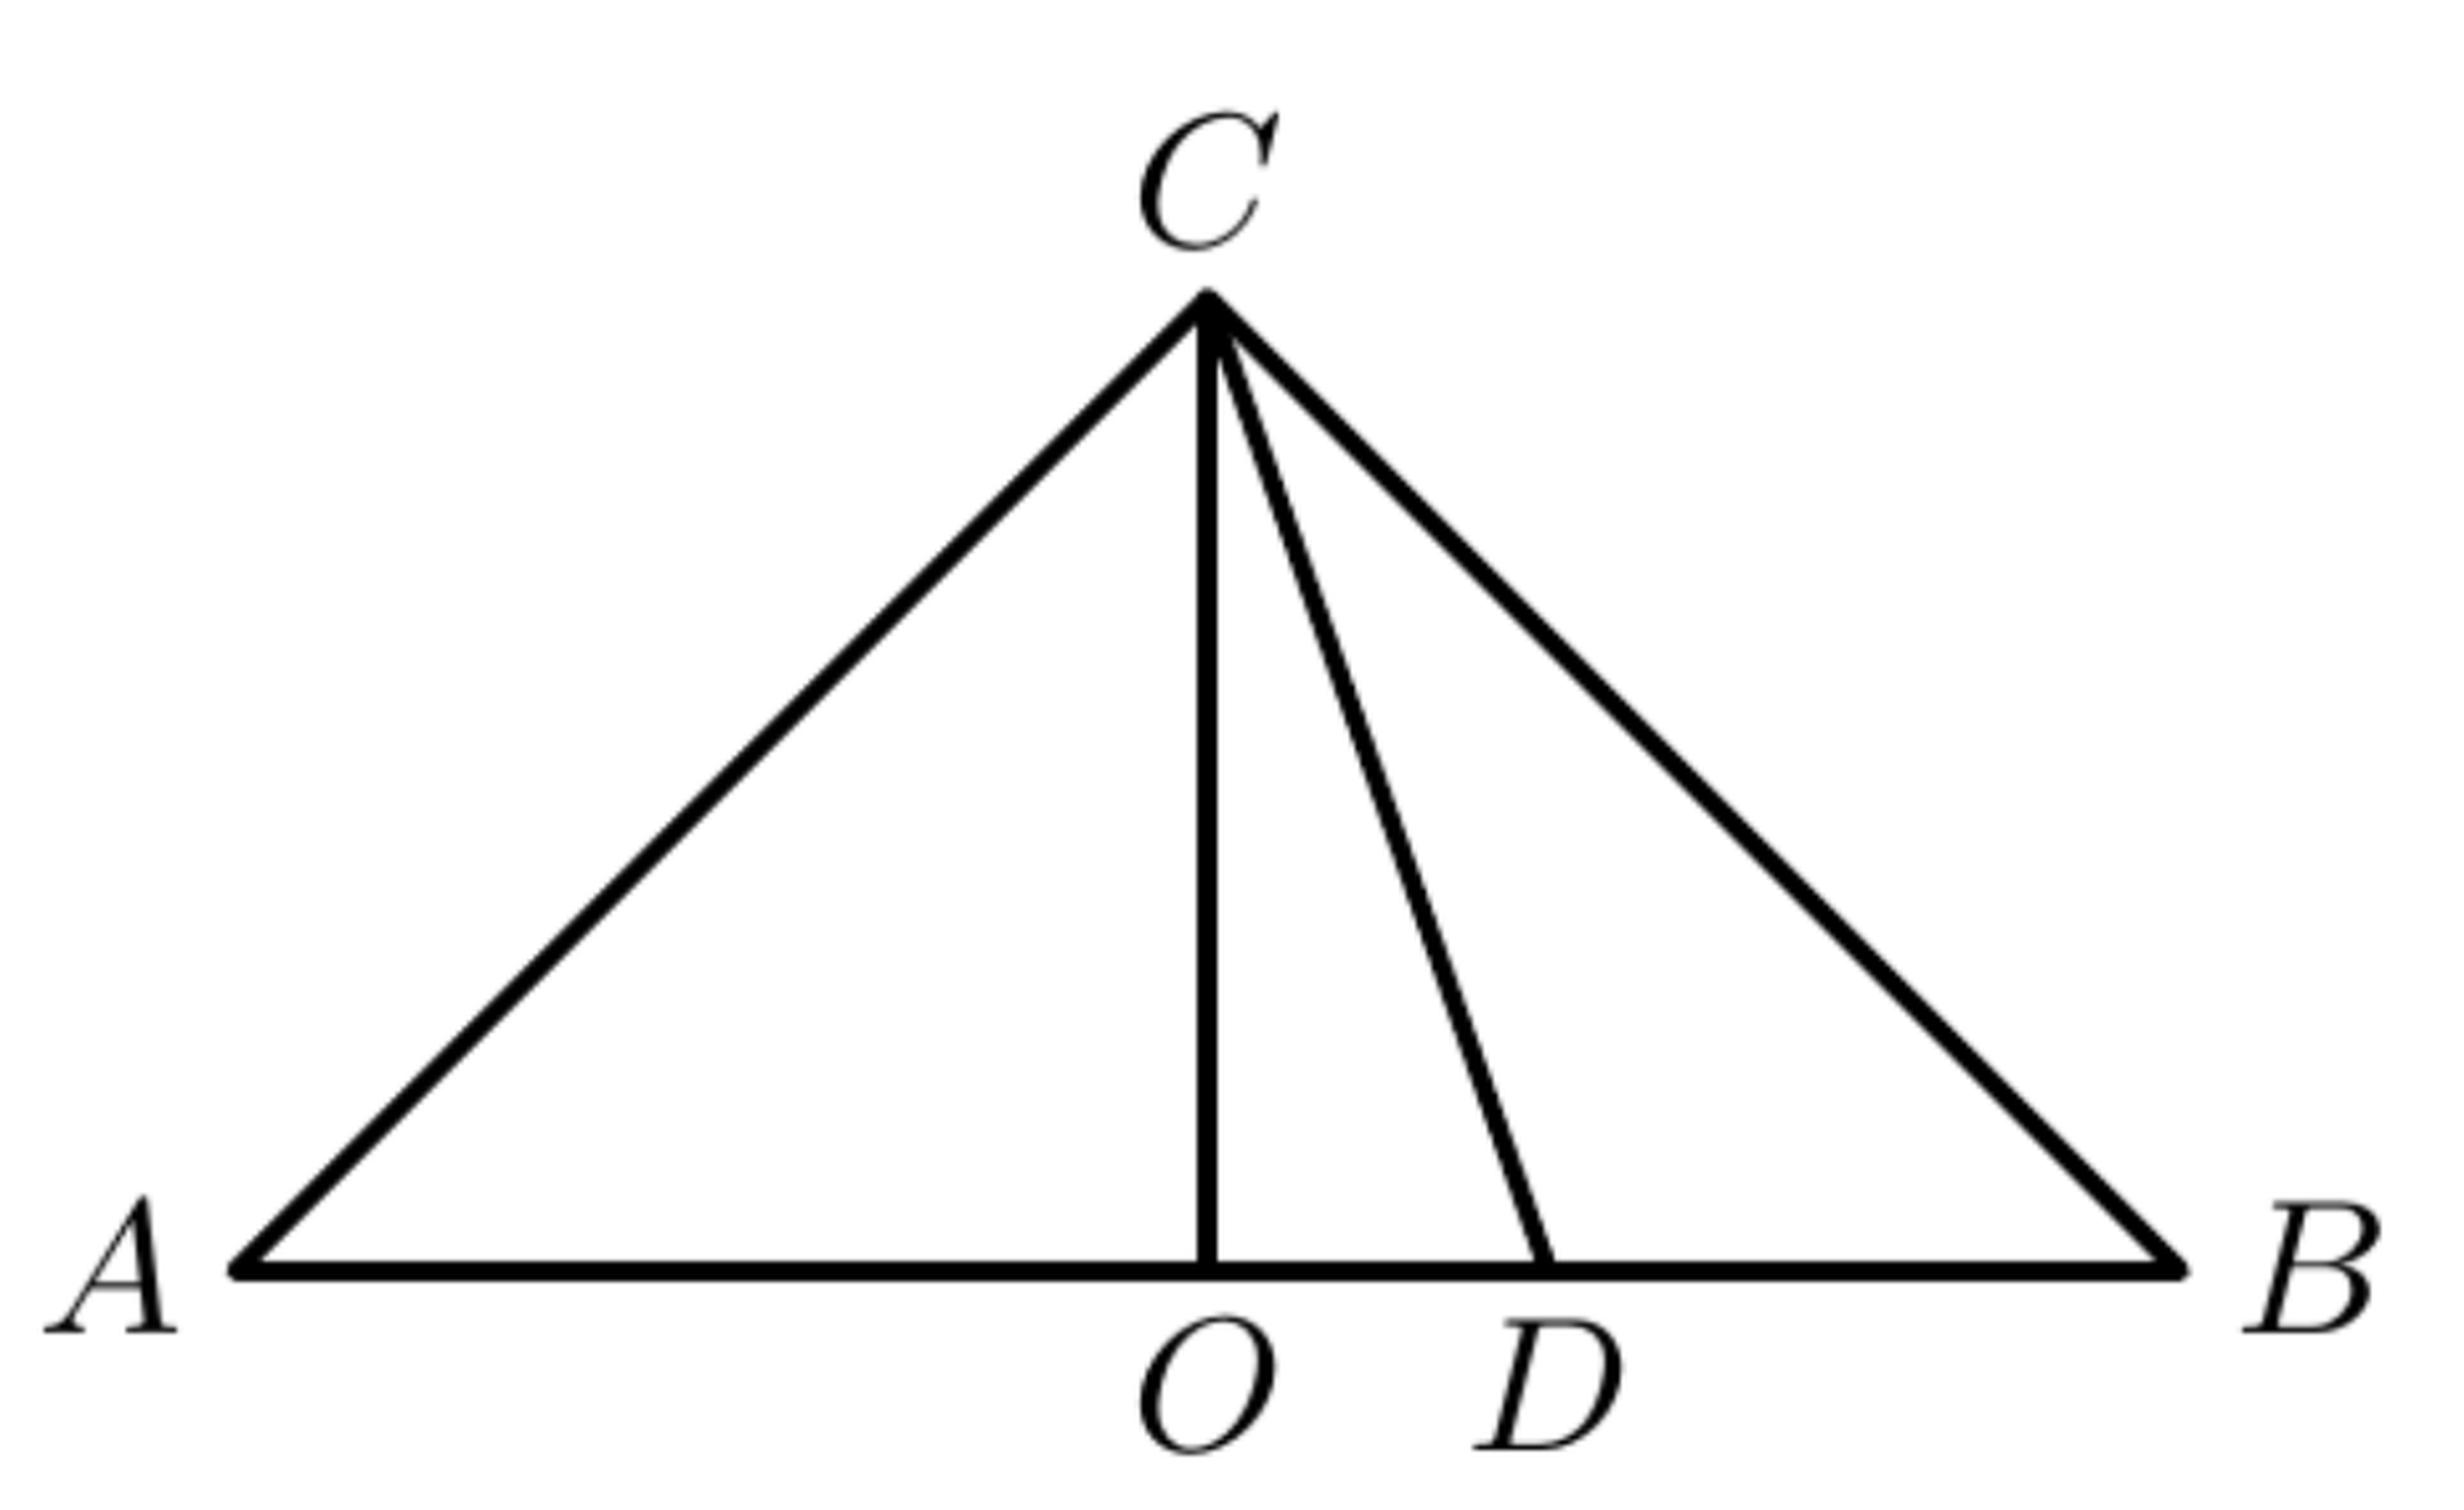
\includegraphics[width=0.34\textwidth]{figures/gao160_q16.png}
\end{center}

\keepwithprev
A. $\dfrac{a+b}{2}\geqslant\sqrt{ab}$ ($a>0,b>0$)\qquad B. $a^2+b^2\geqslant2\sqrt{ab}$ ($a>0,b>0$)

C. $\dfrac{a+b}{2}\leqslant\sqrt{\dfrac{a^2+b^2}{2}}$ ($a>0,b>0$)\qquad D. $\dfrac{2ab}{a+b}\leqslant\sqrt{ab}$ ($a>0,b>0$)

\ifanswer
\solbegin
\step{$CO=AO=\dfrac{a+b}{2},OD=\left\lvert a-\dfrac{a+b}{2}\right\rvert=\dfrac{\lvert a-b\rvert}{2}$，}
\step{$CD=\sqrt{CO^2+OD^2}=\sqrt{\dfrac{a^2+b^2}{2}}\geqslant CO=\dfrac{a+b}{2}$，}
\step{等号当且仅当 $a=b$ 时成立，故选 $C$.}
\solend
\fi

\end{enumerate}

\bigsec{三、解答题}

\begin{enumerate}
\setcounter{enumi}{16}

% === Q17 === cases 块算一行；判别式印等腰偏高三角 \Delta；解析 7 行
\item 已知幂函数 $f(x)=(m^2-2m-2)x^{m-1}$ 在 $(0,+\infty)$ 上是严格增函数.

(1) 求 $m$ 的值；

(2) 若关于 $x$ 的方程 $f(x)=(t+1)x-t^2$ 有两个不相等的正实根，求实数 $t$ 的取值范围.

\ifanswer
\solbegin
\step{(1) 幂函数的系数为 1，因此 $m^2-2m-2=1\Leftrightarrow(m-3)(m+1)=0$，}
\step{解得 $m=3$ 或 $m=-1$.}
\step{由 $f(x)$ 在 $(0,+\infty)$ 上严格递增，得 $m-1>0$，所以 $m=3$，}
\step{此时 $f(x)=x^2$.}
\step{(2) 原方程化为 $x^2-(t+1)x+t^2=0$，}
\step{方程有两个不相等的正实根，则 $\begin{cases}\Delta=(t+1)^2-4t^2=(1-t)(3t+1)>0\\t+1>0\\t^2>0\end{cases}$，}% 判别式原卷印等腰偏高三角 \Delta，照录
\step{得 $t\in\left(-\dfrac{1}{3},0\right)\cup(0,1)$.}
\solend
\fi

% === Q18 === 补集上划线 \overline{A}、\subseteq 带下划线、\varnothing；解析 8 行
\item 已知集合 $A=\{x\mid\lvert x-a\rvert<a-3\}$，$B=\left\{x\mid\dfrac{x+1}{x-2}\geqslant2\right\}$.

(1) 若 $a=5$，求 $\overline{A}\cap B$；

(2) 若 $A\cap B=A$，求实数 $a$ 的取值范围.

\ifanswer
\solbegin
\step{(1) $\dfrac{x+1}{x-2}\geqslant2\Leftrightarrow\dfrac{5-x}{x-2}\geqslant0\Leftrightarrow2<x\leqslant5,B=(2,5]$，}
\step{当 $a=5$ 时，$A=\{x\mid\lvert x-5\rvert<2\}=(3,7)$，于是 $\overline{A}=(-\infty,3]\cup[7,+\infty)$，}
\step{因此 $\overline{A}\cap B=(2,3]$.}
\step{(2) $A\cap B=A$ 等价于 $A\subseteq B$.}
\step{当 $a\leqslant3$ 时，$a-3\leqslant0$，$A=\varnothing$，满足条件.}
\step{当 $a>3$ 时，$\lvert x-a\rvert<a-3\Leftrightarrow3<x<2a-3,A=(3,2a-3)$，}
\step{此时 $A\subseteq B=(2,5]$ 等价于 $2a-3\leqslant5$，即 $a\leqslant4$，结合 $a>3$ 得 $3<a\leqslant4$.}
\step{合并两种情形，实数 $a$ 的取值范围为 $(-\infty,4]$.}
\solend
\fi

% === Q19 === 数据表 tabular 重排（高一130 成例）；cases 块算一行；解析 6 行
\item 作为我国最高水平的综合性运动会，全运会汇聚了国内顶尖体育健儿，某代表队从第 8 届全运会开始登上赛场，且参赛运动员人数逐年递增. 设 $t$ 为该代表队参赛后经过的届数，即第 8 届为 $t=0$，第 9 届为 $t=1$，以此类推. 经过 $t$ 届，运动员人数为 $y$ 人，具体数据如下：

\begin{center}
\begin{tabular}{cccccc}
$t$ & 0 & 1 & 2 & 3 & 4 \\
\hline
届数 & 8 & 9 & 10 & 11 & 12 \\
运动员人数（$y$ 人） & 4 & 11 & 25 & 53 & 109
\end{tabular}
\end{center}

(1) 现有以下两种函数模型：① $y=a\cdot b^t+c$ ($a>0,b>1$)；② $y=\log_a(t+b)+c$ ($b>0,a>1$). 请根据上表中运动员人数的增长规律，选出你认为符合的函数模型（不用说明理由），并利用表中前 3 组数据求出相应的函数解析式；

(2) 若参赛运动员人数按照 (1) 中求得的模型继续增长，在第几届全运会时，该代表队运动员人数将会首次超过 1000 人？

\ifanswer
\solbegin
\step{(1) 选模型①，将前 3 组数据代入，得 $\begin{cases}a+c=4\\ab+c=11\\ab^2+c=25\end{cases}$，}% 原卷印"选模型①"（圈数字①），OCR 误作"四"，照录①，见头注 ⑤ 3
\step{相邻两式相减，得 $a(b-1)=7$，$ab(b-1)=14$，}
\step{两式相除得 $b=2$，进而 $a=7$，$c=-3$，所求函数解析式为 $y=7\cdot2^t-3$.}
\step{(2) $y=7\cdot2^t-3$ 随 $t$ 的增大而增大，且 $t=7$ 时，$y=893<1000$；}
\step{$t=8$ 时，$y=1789>1000$，}
\step{$t$ 为非负整数，首次超过 1000 人时 $t=8$，对应第 $8+8=16$ 届全运会.}
\solend
\fi

% === Q20 === 解析 12 行（跨 08—09 页）
\item 已知函数 $f(x)=\log_a(a-a^x)$.

(1) 求该函数的定义域；

(2) 若 $a>1$，试判断关于 $x$ 的方程 $f(x)=2$ 是否有实数解，并说明理由；

(3) 若当 $x\in(-\infty,0]$ 时，关于 $x$ 的不等式 $f(x)\geqslant-1$ 恒成立，求实数 $a$ 的取值范围.

\ifanswer
\solbegin
\step{(1) 对数的底数须满足 $a>0$ 且 $a\ne1$，真数须满足 $a-a^x>0$，即 $a^x<a^1$.}% 原卷印 $a^1$，照录未化简，见头注 ⑤ 4
\step{当 $a>1$ 时，$x<1$，定义域为 $(-\infty,1)$.}
\step{当 $0<a<1$ 时，$x>1$，定义域为 $(1,+\infty)$.}
\step{(2) 当 $a>1$ 时，若 $f(x)=2$，则 $a-a^x=a^2\Rightarrow a^x=a(1-a)<0$，}
\step{这与 $a^x>0$ 矛盾，因此方程无实数解.}
\step{(3) 不等式在 $(-\infty,0]$ 上恒成立，须先保证该区间包含于函数的定义域，}
\step{由 (1) 得 $a>1$.}
\step{当 $x\leqslant0$ 时，$0<a^x\leqslant1$，所以 $a-a^x\geqslant a-1>0$.}
\step{由对数函数的单调性，$f(x)=\log_a(a-a^x)\geqslant\log_a(a-1)=f(0)$，}
\step{等号当且仅当 $x=0$ 时成立，}
\step{因此所求条件等价于 $\log_a(a-1)\geqslant-1\Leftrightarrow a-1\geqslant\dfrac{1}{a}\Leftrightarrow a^2-a-1\geqslant0$，}
\step{结合 $a>1$，得 $a\in\left[\dfrac{1+\sqrt{5}}{2},+\infty\right)$.}
\solend
\fi

% === Q21 === "和积平衡集"定义证明题；\N；解析 18 行（跨 09—10 页）
\item 已知有限集 $A=\{a_1,a_2,\cdots,a_n\}$ ($n\geqslant2,n\in\N$)，如果 $A$ 中元素 $a_i$ ($i=1,2,3,\cdots,n$) 满足 $a_1+a_2+a_3+\cdots+a_n=a_1\times a_2\times\cdots\times a_n$，就称 $A$ 为“和积平衡集”.

(1) 分别判断集合 $A=\{1,2,3,4\}$，$B=\{4+2\sqrt{2},4-2\sqrt{2}\}$ 是否为“和积平衡集”；

(2) 已知 $a_1$、$a_2$ 是两个不同的正数，且 $\{a_1,a_2\}$ 是“和积平衡集”，请用反证法证明：$a_1$、$a_2$ 至少有一个大于 2；

(3) 若 $a_i\geqslant1$，且 $a_i\in\N$，求所有符合条件的“和积平衡集”.

\ifanswer
\solbegin
\step{(1) 因为 $1+2+3+4=10\ne24=1\times2\times3\times4$，所以 $A$ 不是“和积平衡集”.}
\step{因为 $(4+2\sqrt{2})+(4-2\sqrt{2})=8=(4+2\sqrt{2})(4-2\sqrt{2})$，}
\step{所以 $B$ 是“和积平衡集”.}
\step{(2) 假设 $a_1$、$a_2$ 都不大于 2，则 $\dfrac{1}{a_1}\geqslant\dfrac{1}{2},\dfrac{1}{a_2}\geqslant\dfrac{1}{2}$，}
\step{由于 $a_1\ne a_2$，上述两个不等式至少有一个严格成立.}
\step{而 $a_1+a_2=a_1a_2$，两边除以 $a_1a_2>0$，得 $1=\dfrac{1}{a_1}+\dfrac{1}{a_2}>\dfrac{1}{2}+\dfrac{1}{2}=1$，矛盾，}
\step{所以 $a_1$、$a_2$ 至少有一个大于 2.}
\step{(3) 不妨设 $a_1<a_2<\cdots<a_n$，由各元素均为正整数，得 $a_i\geqslant i$.}
\step{若 $n\geqslant4$，因其余因子均不小于 1，}
\step{有 $a_1a_2\cdots a_n\geqslant a_2a_{n-1}a_n\geqslant2(n-1)a_n>na_n>a_1+a_2+\cdots+a_n$，}
\step{与和积平衡条件矛盾，因此只需讨论 $n=2,3$.}
\step{当 $n=2$ 时，$a_1+a_2=a_1a_2\Leftrightarrow(a_1-1)(a_2-1)=1$，}
\step{两个因子均为非负整数，只能有 $a_1=a_2=2$，与元素互不相同矛盾.}
\step{当 $n=3$ 时，若 $a_1\geqslant2$，则 $a_2\geqslant3$，从而 $a_1a_2a_3\geqslant6a_3>3a_3>a_1+a_2+a_3$，}
\step{矛盾，因此 $a_1=1$.}
\step{此时 $1+a_2+a_3=a_2a_3\Leftrightarrow(a_2-1)(a_3-1)=2$，}
\step{由 $1\leqslant a_2-1<a_3-1$，得 $a_2-1=1$、$a_3-1=2$，即 $a_2=2$、$a_3=3$.}
\step{检验 $1+2+3=1\times2\times3=6$，所求集合为 $\{1,2,3\}$.}
\solend
\fi

\end{enumerate}

\end{document}
"
% 紧凑版：xelatex "\def\iscompact{1}% 高一160_奉贤中学_期中.tex
%   —— 高一上数学"2026-2027 年奉贤中学高一上期中"（试卷版/答案版/紧凑版）
% 试卷版：xelatex 高一160_奉贤中学_期中.tex
% 答案版：xelatex "\def\isanswer{1}\input{高一160_奉贤中学_期中.tex}"
% 紧凑版：xelatex "\def\iscompact{1}\input{高一160_奉贤中学_期中.tex}"
%
% ① 原始材料：微信公众号"魔都数学加油站"文章，连载"27学年高一160"，原卷卷面标题
% "2026-2027 年奉贤中学高一上期中"（卷面未印副标题、未印连载号）。
% 正文为 10 张 PNG 页（01/04/10 为 2560×3620，02/03/05/06/07/08/09 为
% 4762×6735，同一篇各页分辨率混排，逐页按各自分辨率裁图核对）。
% 体例：讲评版——填空 3—12（10 题）、选择 13—16（4 题）、解答 17—21（5 题），
% 共 19 题，自第 3 题起编（1、2 未印在本篇）；19 题逐题印【解析】，无只印【答案】
% 的题；四道选择题答案在解析末句"故选 $B$/$B$/$D$/$C$"，题干括号
% \mbox{（\quad）} 留空、不另提 \ans{}。题目、答案、解析均据原图转录；卷面粉红色
% 水印"魔都数学加油站"及公众号页脚未录入。
% 全卷插图清单（逐页通读 10 页确认）：2 幅，均为题目配图、三版都出——
%   · Q4 韦恩图（01 页右侧：矩形全集 U、两圆 A/B、阴影部分 B∩上划线 A、
%     标注 U/A/B），裁 figures/gao160_q4.png；
%   · Q16 等腰直角三角形 ABC 图（05 页右下：C 顶点、A/O/D/B 共线底边、
%     CO 与 CD 两条线段），裁 figures/gao160_q16.png；
%   两图均取原卷截图 3—4× LANCZOS 放大、去粉色水印、转灰度、autocontrast；
%   Q4 图左侧题干残字"示"、Q16 图左侧题干残字均已裁白。
%   Q19 有一张 3 行数据表（t／届数／运动员人数（y 人），t=0..4），按全稿
%   成例（高一130）用 tabular 重排，不做成 png；其余各页无题目配图、
%   无解析内配图、无其它表格、无"如图"处。
%
% 卷首标题：原卷印作"2026-2027 年奉贤中学高一上期中"，年份区间按全稿惯例排 en dash；
% 原卷卷面未印副标题，本稿按同期中卷知识模块口径补出"集合与常用逻辑用语、不等式、函数"。
%
% ② 与原卷的排版差异／照录项清单：
%   ① 原文从第 3 题起，本稿保留原题号；共 19 题三节，解答题 5 题到 21；
%      三节各自一个 enumerate + \setcounter{enumi}{2}/{12}/{16}（不贯穿），
%      用 \examtitlest[3] 起手；
%   ② 混合体例说明：19 题全印【解析】、用 \solbegin…\solend，无只印【答案】
%      或答案印括号内的题；四道选择题答案在解析末句"故选 $B$/$B$/$D$/$C$"
%      （逐个放大复核）、括号 \mbox{（\quad）} 留空、不另提 \ans{}；答案版
%      【答案】/【解析】标记数 = 19 = 全卷题数（0 个 \ans ＋ 19 个 \solbegin）；
%   ③ 原卷卷面未印副标题，本稿按知识模块口径补出；
%   ④ 原卷填空横线按全稿惯例排 \blankline[4.4em]；选择题括号排 \mbox{（\quad）}、
%      四道选择题的选项段前按惯例各加 \keepwithprev；解答题不留作答区、不加
%      \anspace（原卷为讲评版，109—113 起全稿不用 \anspace）；
%   ⑤ 数集归一：Q4"$U=\Z$"、Q9"$a\in\R$，$b\in\R$"、Q11"$n\in\Z$"、
%      Q15"$s\in\R$"、Q21"$n\in\N$""$a_i\in\N$"原卷印正体粗体 Z/R/N，
%      按全稿惯例归一 \Z／\R／\N；集合描述竖线排 \mid（Q3、Q4、Q12、
%      Q18、Q21）；空集 \varnothing（Q18 解析 (2)）；补集照原卷上划线排
%      \overline{A}（Q4 解析、Q18 (1) 题干与解析）；子集符号 Q18 两处
%      "$A\subseteq B$"印带下划线 ⊆、照录 \subseteq；
%   ⑥ 绝对值排 \lvert…\rvert（Q7、Q8 题干与解析、Q9 题干、Q16 解析、
%      Q18 题干与解析），Q16 解析的 \left\lvert…\right\rvert 与 \lvert…\rvert
%      均在同一 $…$ 组内配对平衡；
%   ⑦ 判别式两形混用逐处照录不统一（放大逐处确认）：Q3 解析
%      "$\triangle=1^2-4a\times\frac{1}{4}=0$"原卷印扁等边三角、照录
%      \triangle；Q17 解析 cases 块"$\Delta=(t+1)^2-4t^2=(1-t)(3t+1)>0$"
%      原卷印等腰偏高三角、照录 \Delta；Q16 题干几何符号"$\triangle ABC$"
%      按全稿几何三角形记号惯例归一 \triangle（参照 高一150／132 成例）；
%   ⑧ 不等号按全稿惯例排 \leqslant／\geqslant；中文弯引号照录：Q9 题干
%      "充分非必要""必要非充分""充要""既非充分又非必要"、Q14 题干
%      "存在 $x\in(1,+\infty)$，使得 $f(x)>0$"与解析"存在""对任意"、
%      Q21 题干与解析多处"和积平衡集"；注释里一律 ASCII 引号；
%   ⑨ 文本圈数字逐处照录：Q12 题干①②③、Q12 解析"故①正确""同②得"
%      "故②正确""③假设""故③错误""故真命题是①②"、Q19 题干①②与解析
%      "选模型①"，均为印刷圈数字（非 \textcircled、非数学模式）；
%   ⑩ 半角逗号在数学组之间是全稿惯例、非笔误，逐处照录（Q8"$2^t,2^{-t}$"、
%      Q9"$a=-1,b=-2$""$a=1,b=-1$"、Q11"$1\leqslant a<10,n\in\Z$"、
%      Q12"$s_1=\frac{1}{2},t_1=x_n$"、Q16 选项"$a>0,b>0$"与解析
%      "$CO=AO=\frac{a+b}{2},OD=...$"、Q18"$2<x\leqslant5,B=(2,5]$"
%      "$3<x<2a-3,A=(3,2a-3)$"、Q21"$n=2,3$"等）；行中全角逗号／顿号
%      照录（Q15 选项"$a>1$，且 $s>0$"、Q12 解析"$s$、$t$"、Q21 解析
%      "$a_1$、$a_2$"），顿号一律移出数学模式；
%   ⑪ "图像／图象"逐处照录：本卷 Q5"的图像恒过一个定点"、Q10"的图像经过点"、
%      Q13 题干两处"图像"与解析"对称图像对应的函数"均印"图像"（有亻）；
%      Q16 印"图形"（利用图形说明、该图形能说明），无"图象"用例；
%   ⑫ 复杂式照录别简化：Q3 $ax^2+x+\frac14=0$、Q5 $y=\log_a(5x-9)-4$、
%      Q6 $(1-2x)^{\frac34}>x^{\frac34}$ 与 $\left[0,\frac12\right]$、
%      Q8 $\frac{s+\sqrt{s^2-4}}{2}$、Q10 $y=\frac{2^x}{2^x+ax}$ 与
%      $\frac{2^p}{2^p+ap}=\frac56$、$\frac{2^q}{2^q+aq}=\frac16$、
%      Q11 $N=a\times10^n$ 与 $3^{2026}$、$2026\lg3\approx966.60$、
%      $966.64512<2026\lg3<966.66538$、Q12 $Y=\{(s,t)\mid s\in X,t\in X\}$
%      与 $\frac12 s+tx_n=0$、Q16 $\sqrt{\frac{a^2+b^2}{2}}$、
%      Q17 $x^2-(t+1)x+t^2=0$ 与 $\left(-\frac13,0\right)\cup(0,1)$、
%      Q18 $\frac{5-x}{x-2}\geqslant0$、Q19 $y=a\cdot b^t+c$ 与
%      $y=\log_a(t+b)+c$、$y=7\cdot2^t-3$、Q20 $f(x)=\log_a(a-a^x)$
%      与 $a^2-a-1\geqslant0$、$\left[\frac{1+\sqrt5}{2},+\infty\right)$、
%      Q21 $4+2\sqrt2$ 与 $(a_2-1)(a_3-1)=2$ 等；
%   ⑬ 子题标号 (1)(2)(3) 按全稿惯例排半角括号；行末／行中句点按全稿惯例
%      排 ASCII `.`（不是全角「．」）；cases 块整体算一个印刷行
%      （Q17 解析、Q19 解析 (1)）；
%   ⑭ 配图：Q4／Q16 题目配图（三版都出）放 \item 内题干之后 \begin{center}，
%      各用 \needvspace{8cm} 守卫把整块推走，**守卫放在 \item 之前**
%      （见 高一153 Q11/Q19 成例与切页审计 B 类坑）；
%   ⑮ 一条 \step = 原卷解析的一个印刷行；跨上下半页的重叠行只算一次
%      （Q4 解析、Q9 解析首行、Q11 解析首行、Q12 解析"若 $s=-1$…"一行、
%      Q18 解析"此时 $A\subseteq B=(2,5]$…"一行、Q20 (2) 题干、
%      Q21 解析"由 $1\leqslant a_2-1<a_3-1$…"一行）；原卷折行别合并；
%   ⑯ Q10 之后另有一整块【注】按语（03 页上半，5 个印刷行），是讲评版作者对
%      原卷数据自相矛盾的加注、不属于任何题的【解析】。本稿按 高一53
%      "注：…"成例放 Q10 的 \solend 之后、Q10 的 \fi 收尾之前：
%      **整块只保留 Q10 那一层外层 \ifanswer**（那个 \fi 就是 Q10 的收尾），
%      块内 \stepm{【注】}{首行} ＋ 4 条 \step 各自自带内层 \ifanswer…\fi
%      （\step／\stepm 宏内自带，源码里不手动再包一层 \ifanswer，
%      否则 题目溯源.py 的 strip_answers 非贪婪正则会错切）；
%      \stepm 第一参数直接用「【注】」作标签，与全稿 \ans 的【答案】、
%      \solbegin 的【解析】同性质，未加粗以外不另加任何样式；
%      5 行仅答案版出、不新增 \item、不影响溯源，头注 ③ 单列登记、
%      不计入 19 题逐题 \step 账；\stepm 把【注】排成加粗着色标签
%      （原卷为黑色加粗），此一处着色差异在此登记；
%   ⑰ 原卷用字照录：Q11"约翰·纳皮尔""莱布尼兹"（原卷作"兹"，非通行"茨"）、
%      "17 世纪的三大数学发明"；Q16"数学说明的方法""点 $D$ 为斜边 $AB$ 上
%      异于顶点的一个动点"；Q19"登上赛场""以此类推"；
%
% ③ 行数复核：一条 \step = 原卷解析的一个印刷行，cases 块作一个印刷行计。
%   逐题数（逐页核对定稿）：Q3：5；Q4：1；Q5：1；Q6：2；Q7：2；Q8：4；
%   Q9：4；Q10：3；Q11：6；Q12：19；Q13：1；Q14：2；Q15：3；Q16：3；
%   Q17：7；Q18：8；Q19：6；Q20：12；Q21：18。
%   合计 107 条 \step（19 题逐题印刷行账），与原卷逐题印刷行相等。
%   **本卷源码 \step 总数 = 19 题逐题合计 107 ＋ Q10 后独立【注】块 5 行
%   = 112 行**（其中 \step 111 条、\stepm 1 条；\stepm 与 4 条 \step 合为
%   【注】块 5 印刷行）。该 5 行不计入「逐题印刷行」账，也不是任何题的
%   【解析】，而是讲评版编者按语；主会话核验脚本按全文统计 \step 时总数会
%   较逐题账多 5，已与主会话对齐、属已知预期而非错误。
%   全卷 19 题均设 \solbegin…\solend，答案版【答案】/【解析】标记数
%   = 19 = 全卷题数。
%
% ④ 页码分布（供回原图复核）：
%   卷首标题＋"一、填空题"＋Q3 题干＋解析 5 行＋Q4 题干＋韦恩图＋解析
%   1 行＋Q5 题干首行在 01 页上半；Q4 解析（重叠）＋Q5 题干续＋解析 1 行＋
%   Q6 题干＋解析 2 行＋Q7 题干＋解析首行在 01 页下半；Q7 解析末行＋
%   Q8 题干＋解析 4 行＋Q9 题干＋解析首行在 02 页上半；Q9 解析（重叠首行）
%   ＋余 3 行＋Q10 题干＋解析 3 行在 02 页下半；【注】按语 5 行＋Q11 题干＋
%   解析首行在 03 页上半；Q11 解析（重叠首行）＋余 5 行＋Q12 题干＋①②
%   在 03 页下半；Q12 ③＋解析前 9 行在 04 页上半；Q12 解析（重叠 2 行）
%   ＋余 8 行在 04 页下半；Q12 解析末 2 行＋"二、选择题"＋Q13 题干＋选项＋
%   解析 1 行＋Q14 题干＋选项＋解析首行在 05 页上半；Q14 解析末行＋
%   Q15 题干＋选项＋解析 3 行＋Q16 题干＋三角形图在 05 页下半；
%   Q16 选项＋解析 3 行＋"三、解答题"＋Q17 题干＋两问在 06 页上半；
%   Q17 解析 7 行在 06 页下半；Q18 题干＋两问＋解析前 7 行＋Q19 题干首行
%   在 07 页上半；Q18 解析末行（重叠）＋Q19 题干＋表格＋两问在 07 页下半；
%   Q19 解析 6 行＋Q20 题干＋(1)(2) 在 08 页上半；Q20 (2)(3) 题干（重叠）
%   ＋解析 8 行在 08 页下半；Q20 解析末 4 行＋Q21 题干＋(1)(2) 在 09 页
%   上半；Q21 (3)＋解析前 7 行在 09 页下半；Q21 解析 (3) 余 10 行在 10 页
%   上半；Q21 末行（重叠）＋"检验 $1+2+3=1\times2\times3=6$，所求集合为
%   $\{1,2,3\}$."在 10 页下半（此后仅水印、无正文）。本稿按题连排，
%   不丢行、不并折行；全卷末题为第 21 题，无附加题节。
%
% ⑤ 存疑照录（放大原图确认，照录未改、正文对应处另有 % 注）：
%   1. Q10【注】按语：讲评版作者据 $a=\sqrt3$ 时 $2^q=\frac{\sqrt3}{5}q<q$
%      与 $2^n\geqslant n+1$ 推出点 $Q$ 不存在、"严格说本题无解"，并注明
%      "原卷数据疑似有误（同型常见题为 $P(p,\frac65)$、$Q(q,-\frac15)$、
%      $2^{p+q}=36pq$，得 $a=6$）"；本稿照录全块、未删未改（见 ② ⑯）。
%   2. Q12 解析 (3) 末段"若 $t=-1$，则 $\frac{1}{2}s=x_n\cdot(-1)$，
%      于是 $s=2x_n>x_n$，也矛盾，"中，等式右端与紧随的结论符号不自洽
%      （按题意应为 $\frac12 s=x_n$ 或 $-\frac12 s=x_n\cdot(-1)$），逐页
%      放大 04 页确认原卷即如此印、无漏看的负号，照录未改，建议主会话
%      回 04 页再放大复核一次；
%   3. Q19 解析 (1) 印"选模型①"（圈数字①，题干只有①②两种模型）；
%      OCR 误作"选模型四"，放大 08 页确认是①、照录①；
%   4. Q20 解析 (1)"即 $a^x<a^1$"末项原卷印 $a^1$（非 $a$），照录未化简；
%   5. Q11 题干"莱布尼兹"原卷作"兹"（非通行"茨"）、"约翰·纳皮尔"用
%      间隔号·，均照录未改；
%   6. Q9 题干"则 $p$ 是 $q$___条件"与解析"故 $p$ 是 $q$ 的充分非必要条件"
%      句式略异，均照录；
%   7. Q19 解析 (1) 用"前 3 组数据"、题干表格列到 $t=4$，照录未补。
%
\documentclass[a4paper,11pt]{article}
\usepackage{common}

\begin{document}

\examtitlest[3]{2026--2027 年奉贤中学高一上期中}{集合与常用逻辑用语、不等式、函数}

\bigsec{一、填空题}

\begin{enumerate}
\setcounter{enumi}{2}

% === Q3 === 解析 5 行；判别式印扁等边三角 \triangle
\item 若集合 $A=\{x\mid ax^2+x+\dfrac{1}{4}=0\}$ 有且仅有两个子集，则实数 $a=$\blankline[4.4em].

\ifanswer
\solbegin
\step{若集合 $A=\{x\mid ax^2+x+\dfrac{1}{4}=0\}$ 有且仅有两个子集，}
\step{所以方程 $ax^2+x+\dfrac{1}{4}=0$ 只有一个实数根，}
\step{当 $a=0$ 时，方程化为 $x+\dfrac{1}{4}=0$，解得 $x=-\dfrac{1}{4}$，符合题意，}
\step{当 $a\ne0$ 时，则 $\triangle=1^2-4a\times\dfrac{1}{4}=0$，解得 $a=1$，}% 判别式原卷印扁等边三角 \triangle，照录
\step{综上所述，实数 $a=0$ 或 1.}
\solend
\fi

% === Q4 === 题目配图（三版都出）；\needvspace 守卫放 \item 之前；补集上划线 \overline{A}；解析 1 行
\needvspace{8cm}
\item 设全集 $U=\Z$，集合 $A=\{x\mid -3<x<1\}$，$B=\{-1,0,1,2\}$，用列举法表示图中阴影部分为\blankline[4.4em].

\begin{center}
% Q4 韦恩图（全集 U、A/B 两圆、阴影 B∩上划线 A）取 01 页右侧，去粉色水印、去色、4× LANCZOS 放大；三版都出
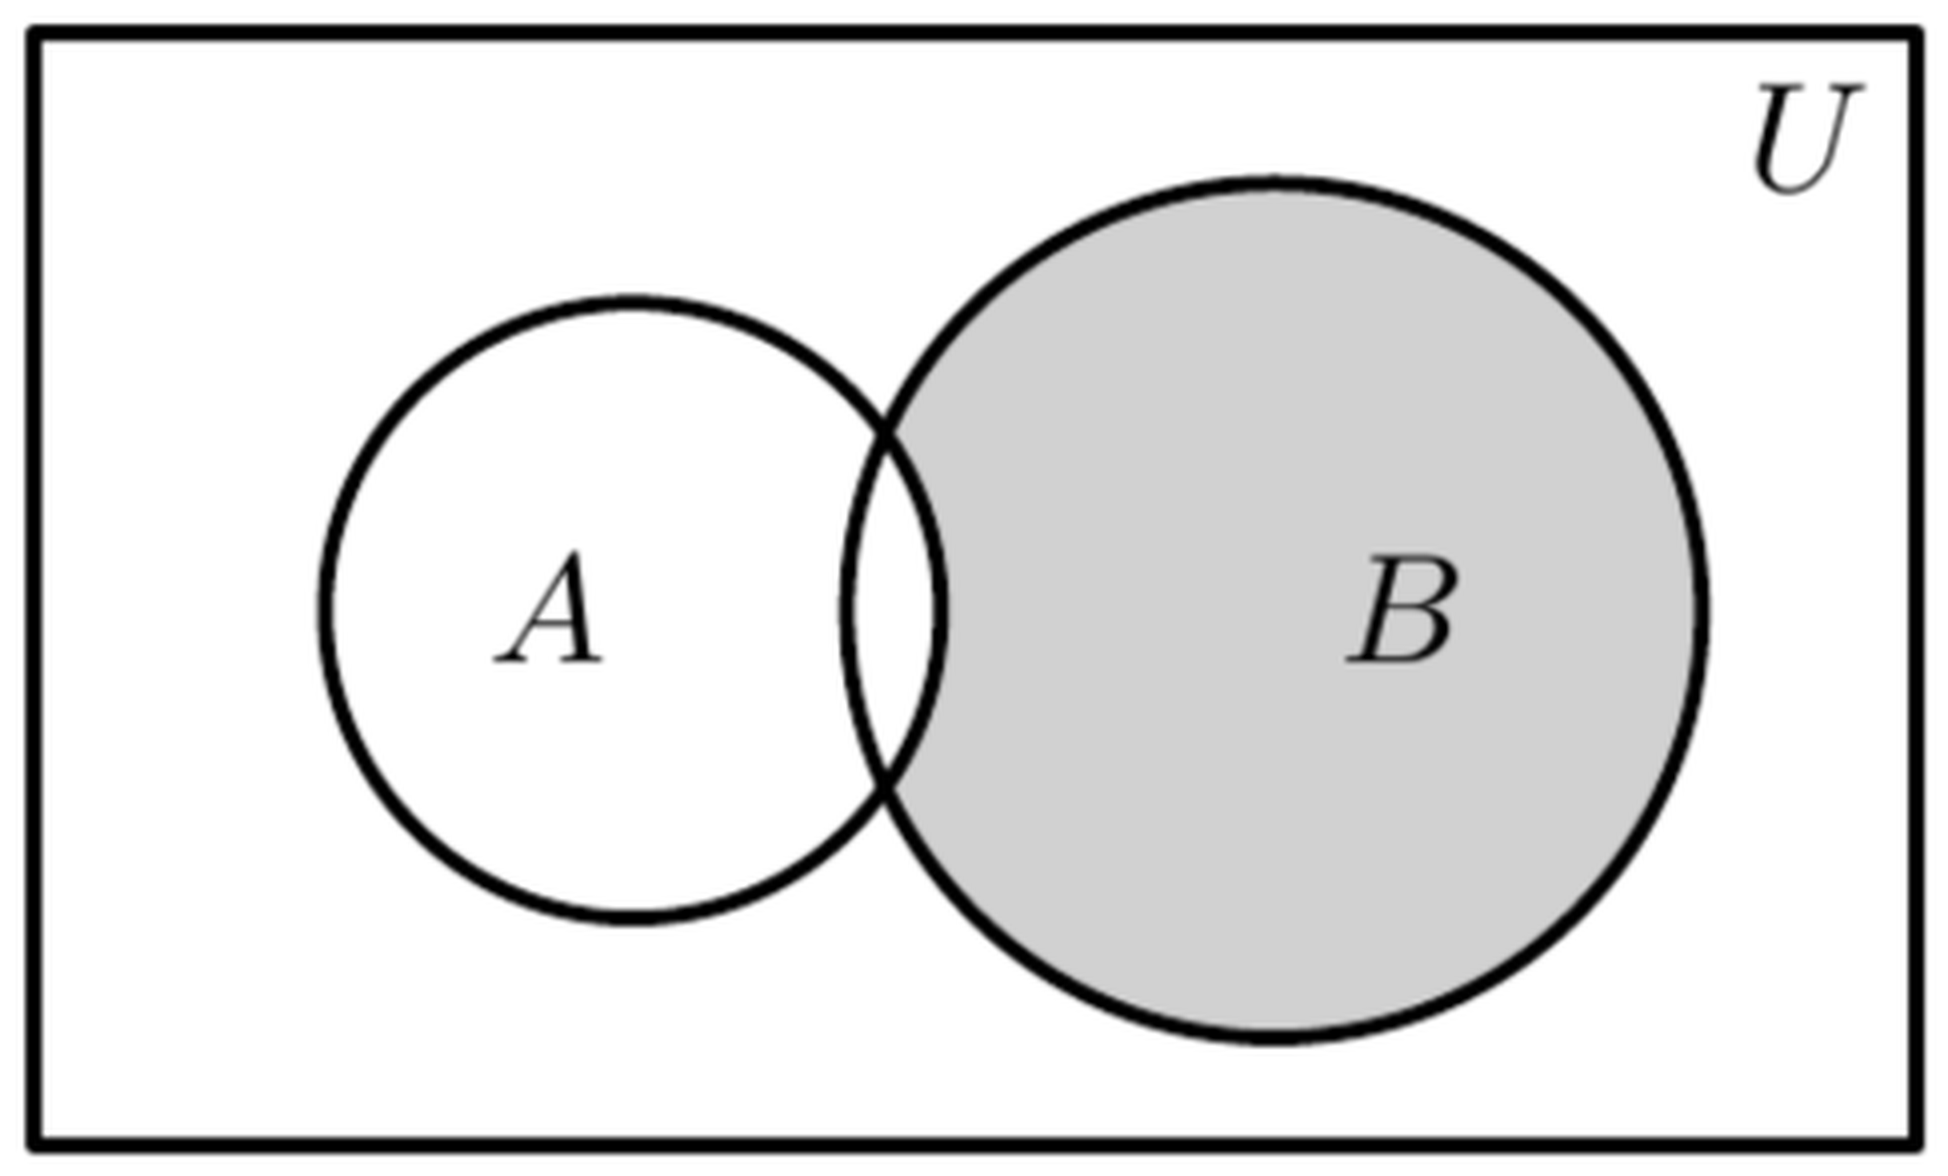
\includegraphics[width=0.38\textwidth]{figures/gao160_q4.png}
\end{center}

\ifanswer
\solbegin
\step{阴影部分表示 $B\cap\overline{A}=\{1,2\}$.}
\solend
\fi

% === Q5 === "图像"（有亻）照录；解析 1 行
\item 已知常数 $a>0$ 且 $a\ne1$，假设无论 $a$ 取何值，函数 $y=\log_a(5x-9)-4$ 的图像恒过一个定点，则这个定点的坐标为\blankline[4.4em].

\ifanswer
\solbegin
\step{$5x-9=1\Rightarrow x=2$，此时 $y=\log_a 1-4=-4$，定点为 $(2,-4)$.}
\solend
\fi

% === Q6 === 解析 2 行
\item 不等式 $(1-2x)^{\frac{3}{4}}>x^{\frac{3}{4}}$ 的解集为\blankline[4.4em].

\ifanswer
\solbegin
\step{定义域为 $\left[0,\dfrac{1}{2}\right]$，由幂函数的单调性，原不等式等价于 $1-2x>x$，}
\step{得 $0\leqslant x<\dfrac{1}{3}$，故解集为 $\left[0,\dfrac{1}{3}\right)$.}
\solend
\fi

% === Q7 === 绝对值 \lvert…\rvert；解析 2 行（跨 01—02 页）
\item 已知不等式 $\lvert x+3\rvert+\lvert x-2\rvert\geqslant 5$，当其等号成立时，$x$ 的取值范围是\blankline[4.4em].

\ifanswer
\solbegin
\step{$\lvert x+3\rvert+\lvert x-2\rvert=\lvert x+3\rvert+\lvert 2-x\rvert\geqslant\lvert(x+3)+(2-x)\rvert=5$，}
\step{等号成立当且仅当 $(x+3)(2-x)\geqslant0$，即 $x\in[-3,2]$.}
\solend
\fi

% === Q8 === 解析 4 行
\item 已知函数 $f(x)=\lvert\log_2 x\rvert$，若方程 $f(x)-t=0$ 有两个不同的实数根 $x_1,x_2$，则 $x_1+x_2$ 的取值范围是\blankline[4.4em].

\ifanswer
\solbegin
\step{方程有两个不同实根，必有 $t>0$，两根为 $2^t,2^{-t}$，}
\step{所以 $x_1+x_2=2^t+2^{-t}>2$（等号仅在 $t=0$ 时成立）.}
\step{任取 $s>2$，令 $a=\dfrac{s+\sqrt{s^2-4}}{2}>1$，取 $t=\log_2 a>0$，则 $x_1+x_2=a+\dfrac{1}{a}=s$，}
\step{所以取值范围为 $(2,+\infty)$.}
\solend
\fi

% === Q9 === 中文弯引号、\R、绝对值 \lvert…\rvert；解析 4 行
\item 已知 $a\in\R$，$b\in\R$，$p:\dfrac{1}{\lvert a\rvert}>\dfrac{1}{\lvert b\rvert}$，$q:\dfrac{1}{a}>\dfrac{1}{b}$，则 $p$ 是 $q$\blankline[4.4em]条件（用“充分非必要”、“必要非充分”、“充要”或“既非充分又非必要”填空）.

\ifanswer
\solbegin
\step{由 $p$、$q$ 中的分式有意义，$a\ne0$ 且 $b\ne0$.}
\step{当 $a=-1,b=-2$ 时，$p$ 成立而 $q$ 不成立，故 $p$ 不是 $q$ 的充分条件.}
\step{当 $a=1,b=-1$ 时，$q$ 成立而 $p$ 不成立，故 $p$ 不是 $q$ 的必要条件.}
\step{故 $p$ 是 $q$ 的充分非必要条件.}
\solend
\fi

% === Q10 === 解析 3 行；其后独立【注】按语 5 行（见头注 ② ⑯、⑤ 1）
\item 已知常数 $a>0$，函数 $y=\dfrac{2^x}{2^x+ax}$ 的图像经过点 $P\left(p,\dfrac{5}{6}\right)$、$Q\left(q,\dfrac{1}{6}\right)$，若 $2^{p+q}=3pq$，则 $a=$\blankline[4.4em].

\ifanswer
\solbegin
\step{由 $\dfrac{2^p}{2^p+ap}=\dfrac{5}{6}$ 得 $2^p=5ap$；由 $\dfrac{2^q}{2^q+aq}=\dfrac{1}{6}$ 得 $2^q=\dfrac{aq}{5}$.}
\step{$2^p>0$，$2^q>0$，$a>0$，得 $p>0$，$q>0$.}
\step{两式相乘得 $2^{p+q}=a^2pq$，又 $2^{p+q}=3pq$ 且 $pq\ne0$，故 $a^2=3$，$a=\sqrt{3}$.}
\solend
% 【注】按语（讲评版编者按，5 个印刷行，仅答案版出，不属于任何题的【解析】）
\stepm{【注】}{按原卷数据严格推敲，点 $Q$ 其实不存在：$a=\sqrt{3}$ 时 $2^q=\dfrac{\sqrt{3}}{5}q<q$；而当 $q>0$}
\step{时，取非负整数 $n$ 使 $n\leqslant q<n+1$，由 $2^{k+1}=2^k+2^k\geqslant2^k+1$ 逐次推得 $2^n\geqslant n+1$，于是}
\step{$2^q\geqslant2^n\geqslant n+1>q$，矛盾. 所以题设条件互相矛盾，严格说本题无解；$\sqrt{3}$ 是由题给关}
\step{系直接推出的值，按命题意图作为答案. 原卷数据疑似有误（同型常见题为 $P\left(p,\dfrac{6}{5}\right)$、}
\step{$Q\left(q,-\dfrac{1}{5}\right)$、$2^{p+q}=36pq$，得 $a=6$）.}% 见头注 ⑤ 1，照录未改
\fi

% === Q11 === 纳皮尔对数材料题；\Z、大数；解析 6 行
\item 17 世纪初，约翰·纳皮尔为了简化计算而发明了对数. 对数的发明是数学史上的重大事件，恩格斯曾经把笛卡尔的坐标系、纳皮尔的对数、牛顿和莱布尼兹的微积分共同称为 17 世纪的三大数学发明. 我们知道，任何一个正实数 $N$ 可以表示成 $N=a\times10^n$ ($1\leqslant a<10,n\in\Z$) 的形式，这便是科学记数法，若两边取常用对数，有 $\lg N=n+\lg a$，则可以估计 $3^{2026}$ 的最高位上的数值为\blankline[4.4em].

\ifanswer
\solbegin
\step{设 $3^{2026}=a\times10^n$ ($1\leqslant a<10,n\in\Z$)，则 $2026\lg 3=n+\lg a$.}
\step{用 $\lg 3\approx 0.4771$ 粗估，得 $2026\lg 3\approx 966.60$.}
\step{为核验误差，用 $0.47712<\lg 3<0.47713$，}
\step{得 $966.64512<2026\lg 3<966.66538$，因此 $n=966$.}
\step{于是 $\lg 4\approx 0.60206<0.64512<\lg a<0.66538<\lg 5\approx 0.69897$，}
\step{所以 $4<a<5$，最高位为 4，估算误差不影响结论.}
\solend
\fi

% === Q12 === 自定义"性质 P"；文本圈数字①②③；解析 19 行（跨 03—05 页）
\item 对于数集 $X=\{-1,x_1,x_2,x_3,\cdots,x_n\}$，其中 $0<x_1<x_2<x_3<\cdots<x_n$，$n\geqslant2$，定义点集 $Y=\{(s,t)\mid s\in X,t\in X\}$，若对于任意 $(s_1,t_1)\in Y$，存在 $(s_2,t_2)\in Y$，使得 $s_1s_2+t_1t_2=0$，则称集合 $X$ 具有性质 $P$. 则下列命题中为真命题的是\blankline[4.4em].

① $X=\{-1,1,2\}$ 具有性质 $P$；②若集合 $X$ 具有性质 $P$，则 $1\in X$；

③集合 $X$ 具有性质 $P$，若 $x_1=\dfrac{1}{2}$，则 $x_n=2$.

\ifanswer
\solbegin
\step{因为 $X=\{-1,1,2\}$，}
\step{所以 $Y=\{(-1,-1),(1,1),(2,2),(-1,1),(-1,2),(1,-1),(1,2),(2,-1),(2,1)\}$，}
\step{由集合 $X$ 具有性质 $P$ 的定义，对于任意 $(s,t)\in Y$，}
\step{若 $s>0$，$t>0$，则 $s=t$ 或 $(s,t)=(1,2)$ 或 $(s,t)=(2,1)$，}
\step{若 $s=t$，取 $s_2=-1$，$t_2=-1$，则 $ss_2+tt_2=0$；}
\step{若 $(s,t)=(1,2)$，取 $s_2=2$，$t_2=-1$，则 $ss_2+tt_2=0$；}
\step{若 $(s,t)=(2,1)$，取 $s_2=-1$，$t_2=2$，则 $ss_2+tt_2=0$；}
\step{若 $s$、$t$ 有一个为负数，则 $s=-1$ 或 $t=-1$，}
\step{若 $s=-1$，则取 $s_2=t$，$t_2=1$，则 $ss_2+tt_2=0$；}
\step{若 $t=-1$，则取 $s_2=1$，$t_2=s$，则 $ss_2+tt_2=0$；故①正确；}
\step{对于任意 $(s_1,t_1)\in Y$，存在 $(s_2,t_2)\in Y$，使得 $s_1s_2+t_1t_2=0$，}
\step{取 $(x_1,x_1)\in Y$，存在 $(x_p,x_q)$ 使得 $x_1x_p+x_1x_q=0$，所以 $x_p+x_q=0$，}
\step{不妨设 $x_p=1$，$x_q=-1$，所以若集合 $X$ 具有性质 $P$，则 $1\in X$，故②正确；}
\step{③假设 $x_n>1$，令 $s_1=\dfrac{1}{2},t_1=x_n$，则存在 $s$、$t\in X$ 使得 $\dfrac{1}{2}s+tx_n=0$，}
\step{同②得 $s$、$t$ 中必有一个数为 $-1$，}
\step{若 $s=-1$，则 $tx_n=\dfrac{1}{2}$，于是 $t=\dfrac{1}{2x_n}<\dfrac{1}{2}=x_1$，矛盾，}
\step{若 $t=-1$，则 $\dfrac{1}{2}s=x_n\cdot(-1)$，于是 $s=2x_n>x_n$，也矛盾，}% 原卷如此（与结论符号不自洽），照录未改，见头注 ⑤ 2
\step{所以 $x_n\leqslant1$，又由②得 $1\in X$，所以 $x_n\geqslant1$，所以 $x_n=1$，故③错误，}
\step{故真命题是①②.}
\solend
\fi

\end{enumerate}

% 答案版里填空解析把页排满，节标题会落到页末、与第 13 题分家（切页审计 B 类）；
% 守卫放 \bigsec 之前，连节标题一起量页高（高一157 成例）
\needvspace{7cm}
\bigsec{二、选择题}

\begin{enumerate}
\setcounter{enumi}{12}

% === Q13 === "图像"照录；解析 1 行，故选 $B$
\item 下列函数中，图像与函数 $y=3^x$ 图像关于 $y$ 轴对称的是\mbox{（\quad）}

\keepwithprev
A. $y=x^3$\qquad B. $y=\left(\dfrac{1}{3}\right)^x$\qquad C. $y=-3^x$\qquad D. $y=\log_3 x$

\ifanswer
\solbegin
\step{将 $x$ 换为 $-x$，得对称图像对应的函数为 $y=3^{-x}=\left(\dfrac{1}{3}\right)^x$，故选 $B$.}
\solend
\fi

% === Q14 === 中文弯引号；解析 2 行（跨 05 页上下），故选 $B$
\item 命题“存在 $x\in(1,+\infty)$，使得 $f(x)>0$”的否定形式为\mbox{（\quad）}

\keepwithprev
A. 不存在 $x\in(-\infty,1]$，使得 $f(x)>0$\qquad B. 对任意 $x\in(1,+\infty)$，有 $f(x)\leqslant0$

C. 对任意 $x\in(-\infty,1]$，有 $f(x)\leqslant0$\qquad D. 存在 $x\in(1,+\infty)$，使得 $f(x)\leqslant0$

\ifanswer
\solbegin
\step{将“存在”改为“对任意”，$x$ 的范围不变，并将 $f(x)>0$ 否定为 $f(x)\leqslant0$，}
\step{故选 $B$.}
\solend
\fi

% === Q15 === \R；四选项两行；解析 3 行，故选 $D$
\item 设 $a>0$，$s\in\R$. 下列各项中，能推出 $a^s>a$ 的一项是\mbox{（\quad）}

\keepwithprev
A. $a>1$，且 $s>0$\qquad B. $a>1$，且 $s<0$

C. $0<a<1$，且 $s>0$\qquad D. $0<a<1$，且 $s<0$

\ifanswer
\solbegin
\step{当 $a>1$ 时，$a^s>a\Leftrightarrow s>1$，A、B 均不能保证.}
\step{当 $0<a<1$ 时，$a^s>a\Leftrightarrow s<1$，C 不能保证，D 中 $s<0<1$，满足要求；}
\step{故选 $D$.}
\solend
\fi

% === Q16 === 题目配图（三版都出）；几何符号 \triangle ABC；解析 3 行，故选 $C$
\needvspace{8cm}
\item 数学说明的方法多种多样，其中利用图形说明就是一种重要方法. 如图所示，在等腰直角三角形 $\triangle ABC$ 中，点 $O$ 为斜边 $AB$ 的中点，点 $D$ 为斜边 $AB$ 上异于顶点的一个动点，设 $AD=a$，$BD=b$，则可用该图形能说明的不等式为\mbox{（\quad）}

\begin{center}
% Q16 等腰直角三角形 ABC 图（C/A/O/D/B 标注）取 05 页右下，去粉色水印、去色、3× LANCZOS 放大；三版都出
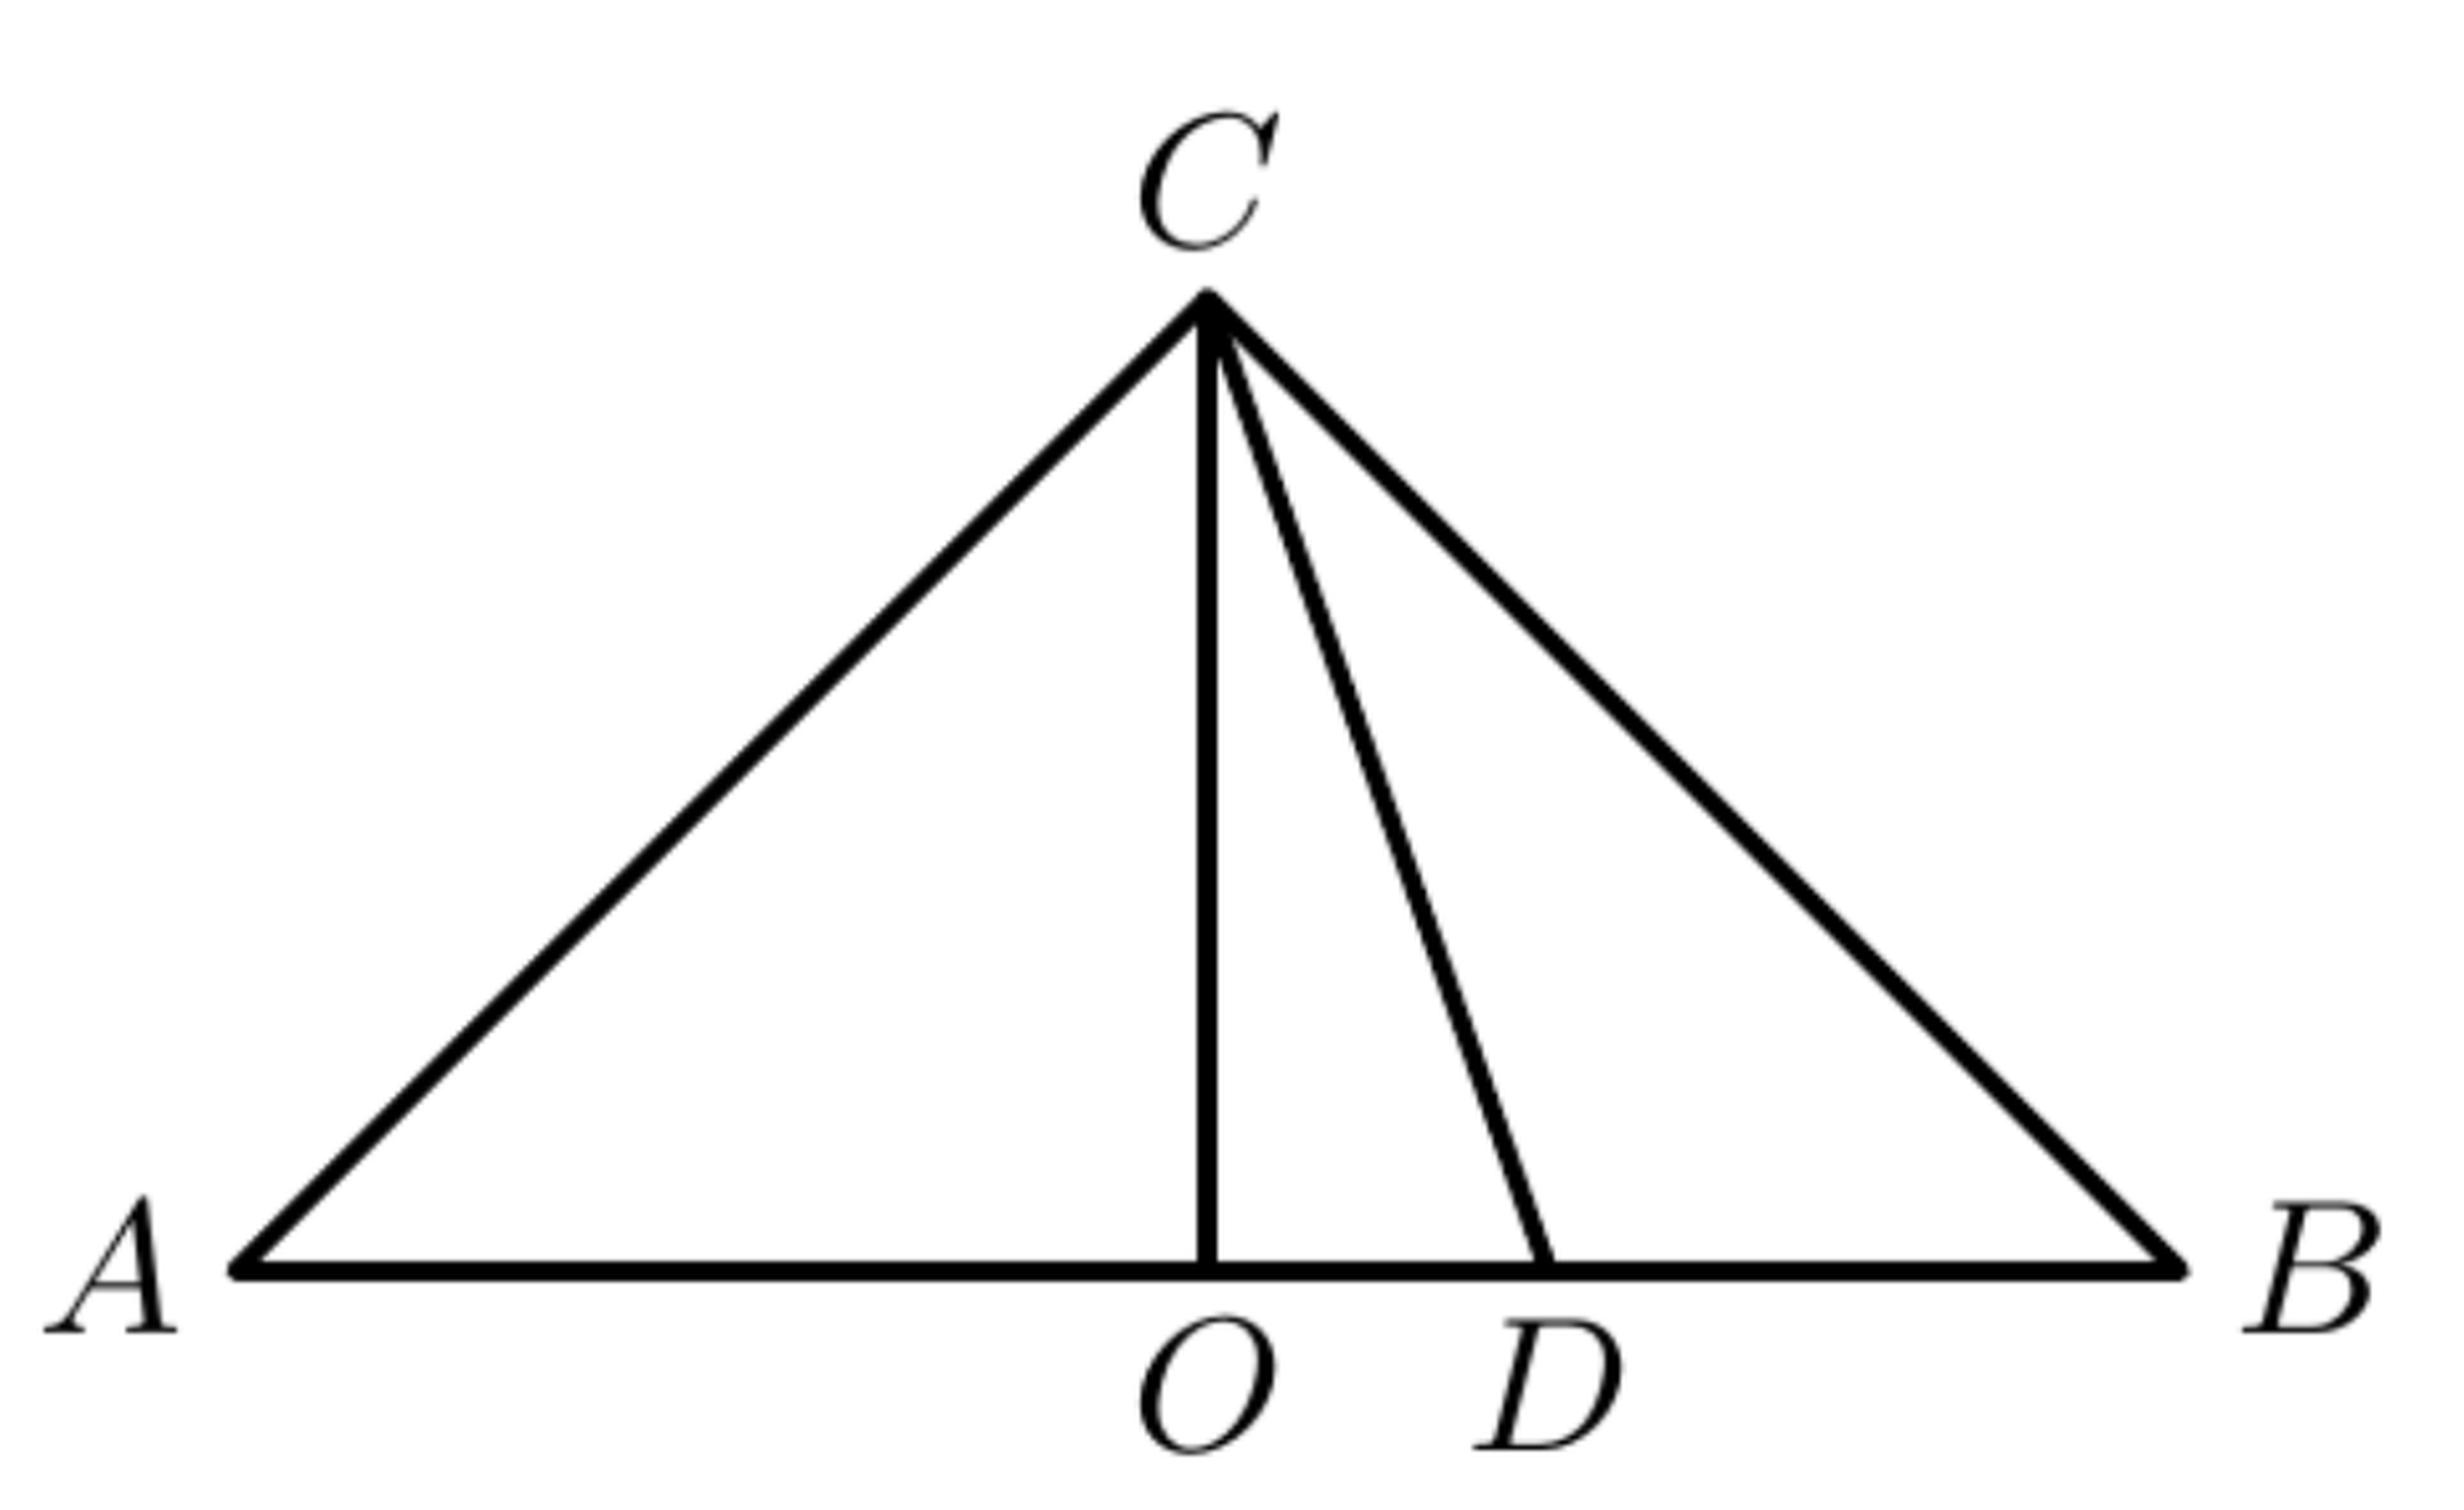
\includegraphics[width=0.34\textwidth]{figures/gao160_q16.png}
\end{center}

\keepwithprev
A. $\dfrac{a+b}{2}\geqslant\sqrt{ab}$ ($a>0,b>0$)\qquad B. $a^2+b^2\geqslant2\sqrt{ab}$ ($a>0,b>0$)

C. $\dfrac{a+b}{2}\leqslant\sqrt{\dfrac{a^2+b^2}{2}}$ ($a>0,b>0$)\qquad D. $\dfrac{2ab}{a+b}\leqslant\sqrt{ab}$ ($a>0,b>0$)

\ifanswer
\solbegin
\step{$CO=AO=\dfrac{a+b}{2},OD=\left\lvert a-\dfrac{a+b}{2}\right\rvert=\dfrac{\lvert a-b\rvert}{2}$，}
\step{$CD=\sqrt{CO^2+OD^2}=\sqrt{\dfrac{a^2+b^2}{2}}\geqslant CO=\dfrac{a+b}{2}$，}
\step{等号当且仅当 $a=b$ 时成立，故选 $C$.}
\solend
\fi

\end{enumerate}

\bigsec{三、解答题}

\begin{enumerate}
\setcounter{enumi}{16}

% === Q17 === cases 块算一行；判别式印等腰偏高三角 \Delta；解析 7 行
\item 已知幂函数 $f(x)=(m^2-2m-2)x^{m-1}$ 在 $(0,+\infty)$ 上是严格增函数.

(1) 求 $m$ 的值；

(2) 若关于 $x$ 的方程 $f(x)=(t+1)x-t^2$ 有两个不相等的正实根，求实数 $t$ 的取值范围.

\ifanswer
\solbegin
\step{(1) 幂函数的系数为 1，因此 $m^2-2m-2=1\Leftrightarrow(m-3)(m+1)=0$，}
\step{解得 $m=3$ 或 $m=-1$.}
\step{由 $f(x)$ 在 $(0,+\infty)$ 上严格递增，得 $m-1>0$，所以 $m=3$，}
\step{此时 $f(x)=x^2$.}
\step{(2) 原方程化为 $x^2-(t+1)x+t^2=0$，}
\step{方程有两个不相等的正实根，则 $\begin{cases}\Delta=(t+1)^2-4t^2=(1-t)(3t+1)>0\\t+1>0\\t^2>0\end{cases}$，}% 判别式原卷印等腰偏高三角 \Delta，照录
\step{得 $t\in\left(-\dfrac{1}{3},0\right)\cup(0,1)$.}
\solend
\fi

% === Q18 === 补集上划线 \overline{A}、\subseteq 带下划线、\varnothing；解析 8 行
\item 已知集合 $A=\{x\mid\lvert x-a\rvert<a-3\}$，$B=\left\{x\mid\dfrac{x+1}{x-2}\geqslant2\right\}$.

(1) 若 $a=5$，求 $\overline{A}\cap B$；

(2) 若 $A\cap B=A$，求实数 $a$ 的取值范围.

\ifanswer
\solbegin
\step{(1) $\dfrac{x+1}{x-2}\geqslant2\Leftrightarrow\dfrac{5-x}{x-2}\geqslant0\Leftrightarrow2<x\leqslant5,B=(2,5]$，}
\step{当 $a=5$ 时，$A=\{x\mid\lvert x-5\rvert<2\}=(3,7)$，于是 $\overline{A}=(-\infty,3]\cup[7,+\infty)$，}
\step{因此 $\overline{A}\cap B=(2,3]$.}
\step{(2) $A\cap B=A$ 等价于 $A\subseteq B$.}
\step{当 $a\leqslant3$ 时，$a-3\leqslant0$，$A=\varnothing$，满足条件.}
\step{当 $a>3$ 时，$\lvert x-a\rvert<a-3\Leftrightarrow3<x<2a-3,A=(3,2a-3)$，}
\step{此时 $A\subseteq B=(2,5]$ 等价于 $2a-3\leqslant5$，即 $a\leqslant4$，结合 $a>3$ 得 $3<a\leqslant4$.}
\step{合并两种情形，实数 $a$ 的取值范围为 $(-\infty,4]$.}
\solend
\fi

% === Q19 === 数据表 tabular 重排（高一130 成例）；cases 块算一行；解析 6 行
\item 作为我国最高水平的综合性运动会，全运会汇聚了国内顶尖体育健儿，某代表队从第 8 届全运会开始登上赛场，且参赛运动员人数逐年递增. 设 $t$ 为该代表队参赛后经过的届数，即第 8 届为 $t=0$，第 9 届为 $t=1$，以此类推. 经过 $t$ 届，运动员人数为 $y$ 人，具体数据如下：

\begin{center}
\begin{tabular}{cccccc}
$t$ & 0 & 1 & 2 & 3 & 4 \\
\hline
届数 & 8 & 9 & 10 & 11 & 12 \\
运动员人数（$y$ 人） & 4 & 11 & 25 & 53 & 109
\end{tabular}
\end{center}

(1) 现有以下两种函数模型：① $y=a\cdot b^t+c$ ($a>0,b>1$)；② $y=\log_a(t+b)+c$ ($b>0,a>1$). 请根据上表中运动员人数的增长规律，选出你认为符合的函数模型（不用说明理由），并利用表中前 3 组数据求出相应的函数解析式；

(2) 若参赛运动员人数按照 (1) 中求得的模型继续增长，在第几届全运会时，该代表队运动员人数将会首次超过 1000 人？

\ifanswer
\solbegin
\step{(1) 选模型①，将前 3 组数据代入，得 $\begin{cases}a+c=4\\ab+c=11\\ab^2+c=25\end{cases}$，}% 原卷印"选模型①"（圈数字①），OCR 误作"四"，照录①，见头注 ⑤ 3
\step{相邻两式相减，得 $a(b-1)=7$，$ab(b-1)=14$，}
\step{两式相除得 $b=2$，进而 $a=7$，$c=-3$，所求函数解析式为 $y=7\cdot2^t-3$.}
\step{(2) $y=7\cdot2^t-3$ 随 $t$ 的增大而增大，且 $t=7$ 时，$y=893<1000$；}
\step{$t=8$ 时，$y=1789>1000$，}
\step{$t$ 为非负整数，首次超过 1000 人时 $t=8$，对应第 $8+8=16$ 届全运会.}
\solend
\fi

% === Q20 === 解析 12 行（跨 08—09 页）
\item 已知函数 $f(x)=\log_a(a-a^x)$.

(1) 求该函数的定义域；

(2) 若 $a>1$，试判断关于 $x$ 的方程 $f(x)=2$ 是否有实数解，并说明理由；

(3) 若当 $x\in(-\infty,0]$ 时，关于 $x$ 的不等式 $f(x)\geqslant-1$ 恒成立，求实数 $a$ 的取值范围.

\ifanswer
\solbegin
\step{(1) 对数的底数须满足 $a>0$ 且 $a\ne1$，真数须满足 $a-a^x>0$，即 $a^x<a^1$.}% 原卷印 $a^1$，照录未化简，见头注 ⑤ 4
\step{当 $a>1$ 时，$x<1$，定义域为 $(-\infty,1)$.}
\step{当 $0<a<1$ 时，$x>1$，定义域为 $(1,+\infty)$.}
\step{(2) 当 $a>1$ 时，若 $f(x)=2$，则 $a-a^x=a^2\Rightarrow a^x=a(1-a)<0$，}
\step{这与 $a^x>0$ 矛盾，因此方程无实数解.}
\step{(3) 不等式在 $(-\infty,0]$ 上恒成立，须先保证该区间包含于函数的定义域，}
\step{由 (1) 得 $a>1$.}
\step{当 $x\leqslant0$ 时，$0<a^x\leqslant1$，所以 $a-a^x\geqslant a-1>0$.}
\step{由对数函数的单调性，$f(x)=\log_a(a-a^x)\geqslant\log_a(a-1)=f(0)$，}
\step{等号当且仅当 $x=0$ 时成立，}
\step{因此所求条件等价于 $\log_a(a-1)\geqslant-1\Leftrightarrow a-1\geqslant\dfrac{1}{a}\Leftrightarrow a^2-a-1\geqslant0$，}
\step{结合 $a>1$，得 $a\in\left[\dfrac{1+\sqrt{5}}{2},+\infty\right)$.}
\solend
\fi

% === Q21 === "和积平衡集"定义证明题；\N；解析 18 行（跨 09—10 页）
\item 已知有限集 $A=\{a_1,a_2,\cdots,a_n\}$ ($n\geqslant2,n\in\N$)，如果 $A$ 中元素 $a_i$ ($i=1,2,3,\cdots,n$) 满足 $a_1+a_2+a_3+\cdots+a_n=a_1\times a_2\times\cdots\times a_n$，就称 $A$ 为“和积平衡集”.

(1) 分别判断集合 $A=\{1,2,3,4\}$，$B=\{4+2\sqrt{2},4-2\sqrt{2}\}$ 是否为“和积平衡集”；

(2) 已知 $a_1$、$a_2$ 是两个不同的正数，且 $\{a_1,a_2\}$ 是“和积平衡集”，请用反证法证明：$a_1$、$a_2$ 至少有一个大于 2；

(3) 若 $a_i\geqslant1$，且 $a_i\in\N$，求所有符合条件的“和积平衡集”.

\ifanswer
\solbegin
\step{(1) 因为 $1+2+3+4=10\ne24=1\times2\times3\times4$，所以 $A$ 不是“和积平衡集”.}
\step{因为 $(4+2\sqrt{2})+(4-2\sqrt{2})=8=(4+2\sqrt{2})(4-2\sqrt{2})$，}
\step{所以 $B$ 是“和积平衡集”.}
\step{(2) 假设 $a_1$、$a_2$ 都不大于 2，则 $\dfrac{1}{a_1}\geqslant\dfrac{1}{2},\dfrac{1}{a_2}\geqslant\dfrac{1}{2}$，}
\step{由于 $a_1\ne a_2$，上述两个不等式至少有一个严格成立.}
\step{而 $a_1+a_2=a_1a_2$，两边除以 $a_1a_2>0$，得 $1=\dfrac{1}{a_1}+\dfrac{1}{a_2}>\dfrac{1}{2}+\dfrac{1}{2}=1$，矛盾，}
\step{所以 $a_1$、$a_2$ 至少有一个大于 2.}
\step{(3) 不妨设 $a_1<a_2<\cdots<a_n$，由各元素均为正整数，得 $a_i\geqslant i$.}
\step{若 $n\geqslant4$，因其余因子均不小于 1，}
\step{有 $a_1a_2\cdots a_n\geqslant a_2a_{n-1}a_n\geqslant2(n-1)a_n>na_n>a_1+a_2+\cdots+a_n$，}
\step{与和积平衡条件矛盾，因此只需讨论 $n=2,3$.}
\step{当 $n=2$ 时，$a_1+a_2=a_1a_2\Leftrightarrow(a_1-1)(a_2-1)=1$，}
\step{两个因子均为非负整数，只能有 $a_1=a_2=2$，与元素互不相同矛盾.}
\step{当 $n=3$ 时，若 $a_1\geqslant2$，则 $a_2\geqslant3$，从而 $a_1a_2a_3\geqslant6a_3>3a_3>a_1+a_2+a_3$，}
\step{矛盾，因此 $a_1=1$.}
\step{此时 $1+a_2+a_3=a_2a_3\Leftrightarrow(a_2-1)(a_3-1)=2$，}
\step{由 $1\leqslant a_2-1<a_3-1$，得 $a_2-1=1$、$a_3-1=2$，即 $a_2=2$、$a_3=3$.}
\step{检验 $1+2+3=1\times2\times3=6$，所求集合为 $\{1,2,3\}$.}
\solend
\fi

\end{enumerate}

\end{document}
"
%
% ① 原始材料：微信公众号"魔都数学加油站"文章，连载"27学年高一160"，原卷卷面标题
% "2026-2027 年奉贤中学高一上期中"（卷面未印副标题、未印连载号）。
% 正文为 10 张 PNG 页（01/04/10 为 2560×3620，02/03/05/06/07/08/09 为
% 4762×6735，同一篇各页分辨率混排，逐页按各自分辨率裁图核对）。
% 体例：讲评版——填空 3—12（10 题）、选择 13—16（4 题）、解答 17—21（5 题），
% 共 19 题，自第 3 题起编（1、2 未印在本篇）；19 题逐题印【解析】，无只印【答案】
% 的题；四道选择题答案在解析末句"故选 $B$/$B$/$D$/$C$"，题干括号
% \mbox{（\quad）} 留空、不另提 \ans{}。题目、答案、解析均据原图转录；卷面粉红色
% 水印"魔都数学加油站"及公众号页脚未录入。
% 全卷插图清单（逐页通读 10 页确认）：2 幅，均为题目配图、三版都出——
%   · Q4 韦恩图（01 页右侧：矩形全集 U、两圆 A/B、阴影部分 B∩上划线 A、
%     标注 U/A/B），裁 figures/gao160_q4.png；
%   · Q16 等腰直角三角形 ABC 图（05 页右下：C 顶点、A/O/D/B 共线底边、
%     CO 与 CD 两条线段），裁 figures/gao160_q16.png；
%   两图均取原卷截图 3—4× LANCZOS 放大、去粉色水印、转灰度、autocontrast；
%   Q4 图左侧题干残字"示"、Q16 图左侧题干残字均已裁白。
%   Q19 有一张 3 行数据表（t／届数／运动员人数（y 人），t=0..4），按全稿
%   成例（高一130）用 tabular 重排，不做成 png；其余各页无题目配图、
%   无解析内配图、无其它表格、无"如图"处。
%
% 卷首标题：原卷印作"2026-2027 年奉贤中学高一上期中"，年份区间按全稿惯例排 en dash；
% 原卷卷面未印副标题，本稿按同期中卷知识模块口径补出"集合与常用逻辑用语、不等式、函数"。
%
% ② 与原卷的排版差异／照录项清单：
%   ① 原文从第 3 题起，本稿保留原题号；共 19 题三节，解答题 5 题到 21；
%      三节各自一个 enumerate + \setcounter{enumi}{2}/{12}/{16}（不贯穿），
%      用 \examtitlest[3] 起手；
%   ② 混合体例说明：19 题全印【解析】、用 \solbegin…\solend，无只印【答案】
%      或答案印括号内的题；四道选择题答案在解析末句"故选 $B$/$B$/$D$/$C$"
%      （逐个放大复核）、括号 \mbox{（\quad）} 留空、不另提 \ans{}；答案版
%      【答案】/【解析】标记数 = 19 = 全卷题数（0 个 \ans ＋ 19 个 \solbegin）；
%   ③ 原卷卷面未印副标题，本稿按知识模块口径补出；
%   ④ 原卷填空横线按全稿惯例排 \blankline[4.4em]；选择题括号排 \mbox{（\quad）}、
%      四道选择题的选项段前按惯例各加 \keepwithprev；解答题不留作答区、不加
%      \anspace（原卷为讲评版，109—113 起全稿不用 \anspace）；
%   ⑤ 数集归一：Q4"$U=\Z$"、Q9"$a\in\R$，$b\in\R$"、Q11"$n\in\Z$"、
%      Q15"$s\in\R$"、Q21"$n\in\N$""$a_i\in\N$"原卷印正体粗体 Z/R/N，
%      按全稿惯例归一 \Z／\R／\N；集合描述竖线排 \mid（Q3、Q4、Q12、
%      Q18、Q21）；空集 \varnothing（Q18 解析 (2)）；补集照原卷上划线排
%      \overline{A}（Q4 解析、Q18 (1) 题干与解析）；子集符号 Q18 两处
%      "$A\subseteq B$"印带下划线 ⊆、照录 \subseteq；
%   ⑥ 绝对值排 \lvert…\rvert（Q7、Q8 题干与解析、Q9 题干、Q16 解析、
%      Q18 题干与解析），Q16 解析的 \left\lvert…\right\rvert 与 \lvert…\rvert
%      均在同一 $…$ 组内配对平衡；
%   ⑦ 判别式两形混用逐处照录不统一（放大逐处确认）：Q3 解析
%      "$\triangle=1^2-4a\times\frac{1}{4}=0$"原卷印扁等边三角、照录
%      \triangle；Q17 解析 cases 块"$\Delta=(t+1)^2-4t^2=(1-t)(3t+1)>0$"
%      原卷印等腰偏高三角、照录 \Delta；Q16 题干几何符号"$\triangle ABC$"
%      按全稿几何三角形记号惯例归一 \triangle（参照 高一150／132 成例）；
%   ⑧ 不等号按全稿惯例排 \leqslant／\geqslant；中文弯引号照录：Q9 题干
%      "充分非必要""必要非充分""充要""既非充分又非必要"、Q14 题干
%      "存在 $x\in(1,+\infty)$，使得 $f(x)>0$"与解析"存在""对任意"、
%      Q21 题干与解析多处"和积平衡集"；注释里一律 ASCII 引号；
%   ⑨ 文本圈数字逐处照录：Q12 题干①②③、Q12 解析"故①正确""同②得"
%      "故②正确""③假设""故③错误""故真命题是①②"、Q19 题干①②与解析
%      "选模型①"，均为印刷圈数字（非 \textcircled、非数学模式）；
%   ⑩ 半角逗号在数学组之间是全稿惯例、非笔误，逐处照录（Q8"$2^t,2^{-t}$"、
%      Q9"$a=-1,b=-2$""$a=1,b=-1$"、Q11"$1\leqslant a<10,n\in\Z$"、
%      Q12"$s_1=\frac{1}{2},t_1=x_n$"、Q16 选项"$a>0,b>0$"与解析
%      "$CO=AO=\frac{a+b}{2},OD=...$"、Q18"$2<x\leqslant5,B=(2,5]$"
%      "$3<x<2a-3,A=(3,2a-3)$"、Q21"$n=2,3$"等）；行中全角逗号／顿号
%      照录（Q15 选项"$a>1$，且 $s>0$"、Q12 解析"$s$、$t$"、Q21 解析
%      "$a_1$、$a_2$"），顿号一律移出数学模式；
%   ⑪ "图像／图象"逐处照录：本卷 Q5"的图像恒过一个定点"、Q10"的图像经过点"、
%      Q13 题干两处"图像"与解析"对称图像对应的函数"均印"图像"（有亻）；
%      Q16 印"图形"（利用图形说明、该图形能说明），无"图象"用例；
%   ⑫ 复杂式照录别简化：Q3 $ax^2+x+\frac14=0$、Q5 $y=\log_a(5x-9)-4$、
%      Q6 $(1-2x)^{\frac34}>x^{\frac34}$ 与 $\left[0,\frac12\right]$、
%      Q8 $\frac{s+\sqrt{s^2-4}}{2}$、Q10 $y=\frac{2^x}{2^x+ax}$ 与
%      $\frac{2^p}{2^p+ap}=\frac56$、$\frac{2^q}{2^q+aq}=\frac16$、
%      Q11 $N=a\times10^n$ 与 $3^{2026}$、$2026\lg3\approx966.60$、
%      $966.64512<2026\lg3<966.66538$、Q12 $Y=\{(s,t)\mid s\in X,t\in X\}$
%      与 $\frac12 s+tx_n=0$、Q16 $\sqrt{\frac{a^2+b^2}{2}}$、
%      Q17 $x^2-(t+1)x+t^2=0$ 与 $\left(-\frac13,0\right)\cup(0,1)$、
%      Q18 $\frac{5-x}{x-2}\geqslant0$、Q19 $y=a\cdot b^t+c$ 与
%      $y=\log_a(t+b)+c$、$y=7\cdot2^t-3$、Q20 $f(x)=\log_a(a-a^x)$
%      与 $a^2-a-1\geqslant0$、$\left[\frac{1+\sqrt5}{2},+\infty\right)$、
%      Q21 $4+2\sqrt2$ 与 $(a_2-1)(a_3-1)=2$ 等；
%   ⑬ 子题标号 (1)(2)(3) 按全稿惯例排半角括号；行末／行中句点按全稿惯例
%      排 ASCII `.`（不是全角「．」）；cases 块整体算一个印刷行
%      （Q17 解析、Q19 解析 (1)）；
%   ⑭ 配图：Q4／Q16 题目配图（三版都出）放 \item 内题干之后 \begin{center}，
%      各用 \needvspace{8cm} 守卫把整块推走，**守卫放在 \item 之前**
%      （见 高一153 Q11/Q19 成例与切页审计 B 类坑）；
%   ⑮ 一条 \step = 原卷解析的一个印刷行；跨上下半页的重叠行只算一次
%      （Q4 解析、Q9 解析首行、Q11 解析首行、Q12 解析"若 $s=-1$…"一行、
%      Q18 解析"此时 $A\subseteq B=(2,5]$…"一行、Q20 (2) 题干、
%      Q21 解析"由 $1\leqslant a_2-1<a_3-1$…"一行）；原卷折行别合并；
%   ⑯ Q10 之后另有一整块【注】按语（03 页上半，5 个印刷行），是讲评版作者对
%      原卷数据自相矛盾的加注、不属于任何题的【解析】。本稿按 高一53
%      "注：…"成例放 Q10 的 \solend 之后、Q10 的 \fi 收尾之前：
%      **整块只保留 Q10 那一层外层 \ifanswer**（那个 \fi 就是 Q10 的收尾），
%      块内 \stepm{【注】}{首行} ＋ 4 条 \step 各自自带内层 \ifanswer…\fi
%      （\step／\stepm 宏内自带，源码里不手动再包一层 \ifanswer，
%      否则 题目溯源.py 的 strip_answers 非贪婪正则会错切）；
%      \stepm 第一参数直接用「【注】」作标签，与全稿 \ans 的【答案】、
%      \solbegin 的【解析】同性质，未加粗以外不另加任何样式；
%      5 行仅答案版出、不新增 \item、不影响溯源，头注 ③ 单列登记、
%      不计入 19 题逐题 \step 账；\stepm 把【注】排成加粗着色标签
%      （原卷为黑色加粗），此一处着色差异在此登记；
%   ⑰ 原卷用字照录：Q11"约翰·纳皮尔""莱布尼兹"（原卷作"兹"，非通行"茨"）、
%      "17 世纪的三大数学发明"；Q16"数学说明的方法""点 $D$ 为斜边 $AB$ 上
%      异于顶点的一个动点"；Q19"登上赛场""以此类推"；
%
% ③ 行数复核：一条 \step = 原卷解析的一个印刷行，cases 块作一个印刷行计。
%   逐题数（逐页核对定稿）：Q3：5；Q4：1；Q5：1；Q6：2；Q7：2；Q8：4；
%   Q9：4；Q10：3；Q11：6；Q12：19；Q13：1；Q14：2；Q15：3；Q16：3；
%   Q17：7；Q18：8；Q19：6；Q20：12；Q21：18。
%   合计 107 条 \step（19 题逐题印刷行账），与原卷逐题印刷行相等。
%   **本卷源码 \step 总数 = 19 题逐题合计 107 ＋ Q10 后独立【注】块 5 行
%   = 112 行**（其中 \step 111 条、\stepm 1 条；\stepm 与 4 条 \step 合为
%   【注】块 5 印刷行）。该 5 行不计入「逐题印刷行」账，也不是任何题的
%   【解析】，而是讲评版编者按语；主会话核验脚本按全文统计 \step 时总数会
%   较逐题账多 5，已与主会话对齐、属已知预期而非错误。
%   全卷 19 题均设 \solbegin…\solend，答案版【答案】/【解析】标记数
%   = 19 = 全卷题数。
%
% ④ 页码分布（供回原图复核）：
%   卷首标题＋"一、填空题"＋Q3 题干＋解析 5 行＋Q4 题干＋韦恩图＋解析
%   1 行＋Q5 题干首行在 01 页上半；Q4 解析（重叠）＋Q5 题干续＋解析 1 行＋
%   Q6 题干＋解析 2 行＋Q7 题干＋解析首行在 01 页下半；Q7 解析末行＋
%   Q8 题干＋解析 4 行＋Q9 题干＋解析首行在 02 页上半；Q9 解析（重叠首行）
%   ＋余 3 行＋Q10 题干＋解析 3 行在 02 页下半；【注】按语 5 行＋Q11 题干＋
%   解析首行在 03 页上半；Q11 解析（重叠首行）＋余 5 行＋Q12 题干＋①②
%   在 03 页下半；Q12 ③＋解析前 9 行在 04 页上半；Q12 解析（重叠 2 行）
%   ＋余 8 行在 04 页下半；Q12 解析末 2 行＋"二、选择题"＋Q13 题干＋选项＋
%   解析 1 行＋Q14 题干＋选项＋解析首行在 05 页上半；Q14 解析末行＋
%   Q15 题干＋选项＋解析 3 行＋Q16 题干＋三角形图在 05 页下半；
%   Q16 选项＋解析 3 行＋"三、解答题"＋Q17 题干＋两问在 06 页上半；
%   Q17 解析 7 行在 06 页下半；Q18 题干＋两问＋解析前 7 行＋Q19 题干首行
%   在 07 页上半；Q18 解析末行（重叠）＋Q19 题干＋表格＋两问在 07 页下半；
%   Q19 解析 6 行＋Q20 题干＋(1)(2) 在 08 页上半；Q20 (2)(3) 题干（重叠）
%   ＋解析 8 行在 08 页下半；Q20 解析末 4 行＋Q21 题干＋(1)(2) 在 09 页
%   上半；Q21 (3)＋解析前 7 行在 09 页下半；Q21 解析 (3) 余 10 行在 10 页
%   上半；Q21 末行（重叠）＋"检验 $1+2+3=1\times2\times3=6$，所求集合为
%   $\{1,2,3\}$."在 10 页下半（此后仅水印、无正文）。本稿按题连排，
%   不丢行、不并折行；全卷末题为第 21 题，无附加题节。
%
% ⑤ 存疑照录（放大原图确认，照录未改、正文对应处另有 % 注）：
%   1. Q10【注】按语：讲评版作者据 $a=\sqrt3$ 时 $2^q=\frac{\sqrt3}{5}q<q$
%      与 $2^n\geqslant n+1$ 推出点 $Q$ 不存在、"严格说本题无解"，并注明
%      "原卷数据疑似有误（同型常见题为 $P(p,\frac65)$、$Q(q,-\frac15)$、
%      $2^{p+q}=36pq$，得 $a=6$）"；本稿照录全块、未删未改（见 ② ⑯）。
%   2. Q12 解析 (3) 末段"若 $t=-1$，则 $\frac{1}{2}s=x_n\cdot(-1)$，
%      于是 $s=2x_n>x_n$，也矛盾，"中，等式右端与紧随的结论符号不自洽
%      （按题意应为 $\frac12 s=x_n$ 或 $-\frac12 s=x_n\cdot(-1)$），逐页
%      放大 04 页确认原卷即如此印、无漏看的负号，照录未改，建议主会话
%      回 04 页再放大复核一次；
%   3. Q19 解析 (1) 印"选模型①"（圈数字①，题干只有①②两种模型）；
%      OCR 误作"选模型四"，放大 08 页确认是①、照录①；
%   4. Q20 解析 (1)"即 $a^x<a^1$"末项原卷印 $a^1$（非 $a$），照录未化简；
%   5. Q11 题干"莱布尼兹"原卷作"兹"（非通行"茨"）、"约翰·纳皮尔"用
%      间隔号·，均照录未改；
%   6. Q9 题干"则 $p$ 是 $q$___条件"与解析"故 $p$ 是 $q$ 的充分非必要条件"
%      句式略异，均照录；
%   7. Q19 解析 (1) 用"前 3 组数据"、题干表格列到 $t=4$，照录未补。
%
\documentclass[a4paper,11pt]{article}
\usepackage{common}

\begin{document}

\examtitlest[3]{2026--2027 年奉贤中学高一上期中}{集合与常用逻辑用语、不等式、函数}

\bigsec{一、填空题}

\begin{enumerate}
\setcounter{enumi}{2}

% === Q3 === 解析 5 行；判别式印扁等边三角 \triangle
\item 若集合 $A=\{x\mid ax^2+x+\dfrac{1}{4}=0\}$ 有且仅有两个子集，则实数 $a=$\blankline[4.4em].

\ifanswer
\solbegin
\step{若集合 $A=\{x\mid ax^2+x+\dfrac{1}{4}=0\}$ 有且仅有两个子集，}
\step{所以方程 $ax^2+x+\dfrac{1}{4}=0$ 只有一个实数根，}
\step{当 $a=0$ 时，方程化为 $x+\dfrac{1}{4}=0$，解得 $x=-\dfrac{1}{4}$，符合题意，}
\step{当 $a\ne0$ 时，则 $\triangle=1^2-4a\times\dfrac{1}{4}=0$，解得 $a=1$，}% 判别式原卷印扁等边三角 \triangle，照录
\step{综上所述，实数 $a=0$ 或 1.}
\solend
\fi

% === Q4 === 题目配图（三版都出）；\needvspace 守卫放 \item 之前；补集上划线 \overline{A}；解析 1 行
\needvspace{8cm}
\item 设全集 $U=\Z$，集合 $A=\{x\mid -3<x<1\}$，$B=\{-1,0,1,2\}$，用列举法表示图中阴影部分为\blankline[4.4em].

\begin{center}
% Q4 韦恩图（全集 U、A/B 两圆、阴影 B∩上划线 A）取 01 页右侧，去粉色水印、去色、4× LANCZOS 放大；三版都出
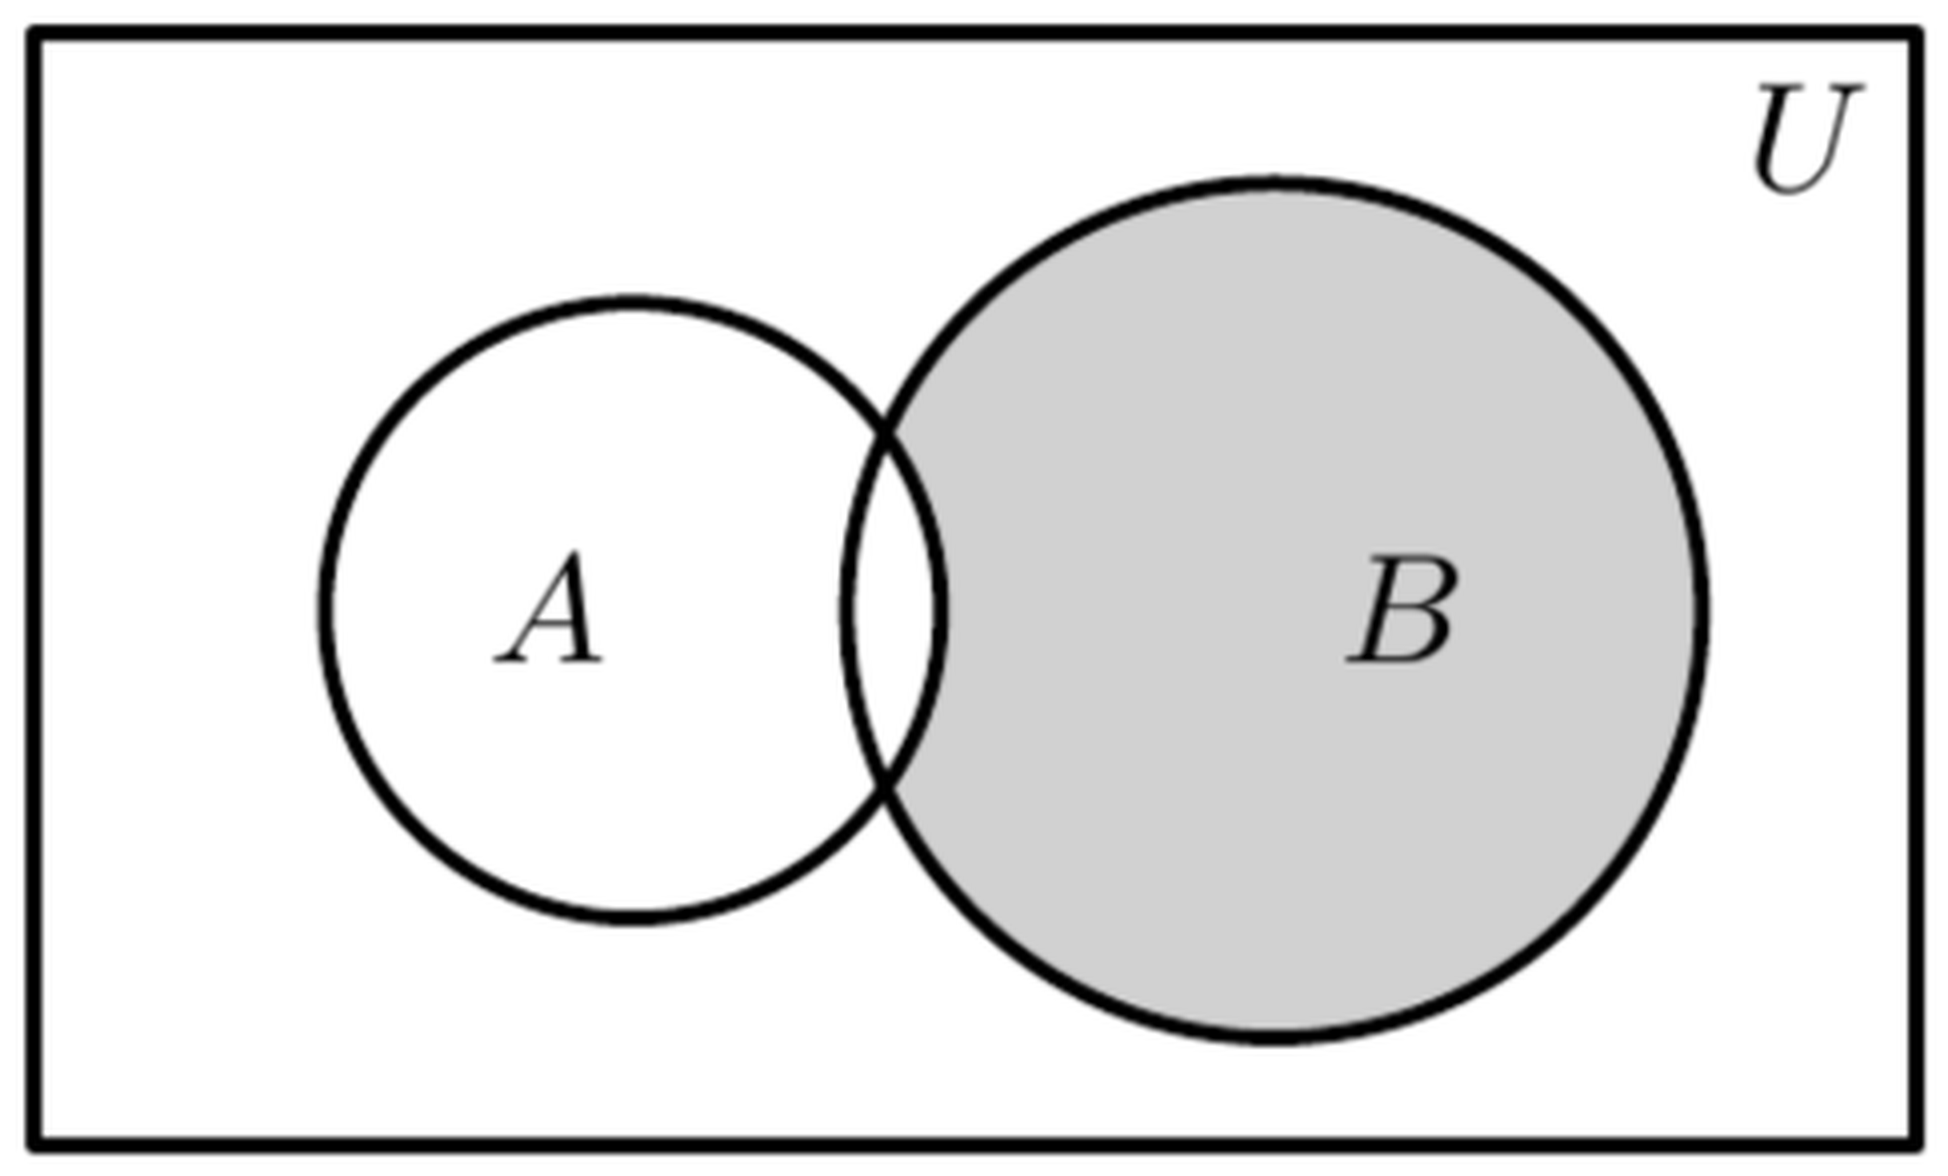
\includegraphics[width=0.38\textwidth]{figures/gao160_q4.png}
\end{center}

\ifanswer
\solbegin
\step{阴影部分表示 $B\cap\overline{A}=\{1,2\}$.}
\solend
\fi

% === Q5 === "图像"（有亻）照录；解析 1 行
\item 已知常数 $a>0$ 且 $a\ne1$，假设无论 $a$ 取何值，函数 $y=\log_a(5x-9)-4$ 的图像恒过一个定点，则这个定点的坐标为\blankline[4.4em].

\ifanswer
\solbegin
\step{$5x-9=1\Rightarrow x=2$，此时 $y=\log_a 1-4=-4$，定点为 $(2,-4)$.}
\solend
\fi

% === Q6 === 解析 2 行
\item 不等式 $(1-2x)^{\frac{3}{4}}>x^{\frac{3}{4}}$ 的解集为\blankline[4.4em].

\ifanswer
\solbegin
\step{定义域为 $\left[0,\dfrac{1}{2}\right]$，由幂函数的单调性，原不等式等价于 $1-2x>x$，}
\step{得 $0\leqslant x<\dfrac{1}{3}$，故解集为 $\left[0,\dfrac{1}{3}\right)$.}
\solend
\fi

% === Q7 === 绝对值 \lvert…\rvert；解析 2 行（跨 01—02 页）
\item 已知不等式 $\lvert x+3\rvert+\lvert x-2\rvert\geqslant 5$，当其等号成立时，$x$ 的取值范围是\blankline[4.4em].

\ifanswer
\solbegin
\step{$\lvert x+3\rvert+\lvert x-2\rvert=\lvert x+3\rvert+\lvert 2-x\rvert\geqslant\lvert(x+3)+(2-x)\rvert=5$，}
\step{等号成立当且仅当 $(x+3)(2-x)\geqslant0$，即 $x\in[-3,2]$.}
\solend
\fi

% === Q8 === 解析 4 行
\item 已知函数 $f(x)=\lvert\log_2 x\rvert$，若方程 $f(x)-t=0$ 有两个不同的实数根 $x_1,x_2$，则 $x_1+x_2$ 的取值范围是\blankline[4.4em].

\ifanswer
\solbegin
\step{方程有两个不同实根，必有 $t>0$，两根为 $2^t,2^{-t}$，}
\step{所以 $x_1+x_2=2^t+2^{-t}>2$（等号仅在 $t=0$ 时成立）.}
\step{任取 $s>2$，令 $a=\dfrac{s+\sqrt{s^2-4}}{2}>1$，取 $t=\log_2 a>0$，则 $x_1+x_2=a+\dfrac{1}{a}=s$，}
\step{所以取值范围为 $(2,+\infty)$.}
\solend
\fi

% === Q9 === 中文弯引号、\R、绝对值 \lvert…\rvert；解析 4 行
\item 已知 $a\in\R$，$b\in\R$，$p:\dfrac{1}{\lvert a\rvert}>\dfrac{1}{\lvert b\rvert}$，$q:\dfrac{1}{a}>\dfrac{1}{b}$，则 $p$ 是 $q$\blankline[4.4em]条件（用“充分非必要”、“必要非充分”、“充要”或“既非充分又非必要”填空）.

\ifanswer
\solbegin
\step{由 $p$、$q$ 中的分式有意义，$a\ne0$ 且 $b\ne0$.}
\step{当 $a=-1,b=-2$ 时，$p$ 成立而 $q$ 不成立，故 $p$ 不是 $q$ 的充分条件.}
\step{当 $a=1,b=-1$ 时，$q$ 成立而 $p$ 不成立，故 $p$ 不是 $q$ 的必要条件.}
\step{故 $p$ 是 $q$ 的充分非必要条件.}
\solend
\fi

% === Q10 === 解析 3 行；其后独立【注】按语 5 行（见头注 ② ⑯、⑤ 1）
\item 已知常数 $a>0$，函数 $y=\dfrac{2^x}{2^x+ax}$ 的图像经过点 $P\left(p,\dfrac{5}{6}\right)$、$Q\left(q,\dfrac{1}{6}\right)$，若 $2^{p+q}=3pq$，则 $a=$\blankline[4.4em].

\ifanswer
\solbegin
\step{由 $\dfrac{2^p}{2^p+ap}=\dfrac{5}{6}$ 得 $2^p=5ap$；由 $\dfrac{2^q}{2^q+aq}=\dfrac{1}{6}$ 得 $2^q=\dfrac{aq}{5}$.}
\step{$2^p>0$，$2^q>0$，$a>0$，得 $p>0$，$q>0$.}
\step{两式相乘得 $2^{p+q}=a^2pq$，又 $2^{p+q}=3pq$ 且 $pq\ne0$，故 $a^2=3$，$a=\sqrt{3}$.}
\solend
% 【注】按语（讲评版编者按，5 个印刷行，仅答案版出，不属于任何题的【解析】）
\stepm{【注】}{按原卷数据严格推敲，点 $Q$ 其实不存在：$a=\sqrt{3}$ 时 $2^q=\dfrac{\sqrt{3}}{5}q<q$；而当 $q>0$}
\step{时，取非负整数 $n$ 使 $n\leqslant q<n+1$，由 $2^{k+1}=2^k+2^k\geqslant2^k+1$ 逐次推得 $2^n\geqslant n+1$，于是}
\step{$2^q\geqslant2^n\geqslant n+1>q$，矛盾. 所以题设条件互相矛盾，严格说本题无解；$\sqrt{3}$ 是由题给关}
\step{系直接推出的值，按命题意图作为答案. 原卷数据疑似有误（同型常见题为 $P\left(p,\dfrac{6}{5}\right)$、}
\step{$Q\left(q,-\dfrac{1}{5}\right)$、$2^{p+q}=36pq$，得 $a=6$）.}% 见头注 ⑤ 1，照录未改
\fi

% === Q11 === 纳皮尔对数材料题；\Z、大数；解析 6 行
\item 17 世纪初，约翰·纳皮尔为了简化计算而发明了对数. 对数的发明是数学史上的重大事件，恩格斯曾经把笛卡尔的坐标系、纳皮尔的对数、牛顿和莱布尼兹的微积分共同称为 17 世纪的三大数学发明. 我们知道，任何一个正实数 $N$ 可以表示成 $N=a\times10^n$ ($1\leqslant a<10,n\in\Z$) 的形式，这便是科学记数法，若两边取常用对数，有 $\lg N=n+\lg a$，则可以估计 $3^{2026}$ 的最高位上的数值为\blankline[4.4em].

\ifanswer
\solbegin
\step{设 $3^{2026}=a\times10^n$ ($1\leqslant a<10,n\in\Z$)，则 $2026\lg 3=n+\lg a$.}
\step{用 $\lg 3\approx 0.4771$ 粗估，得 $2026\lg 3\approx 966.60$.}
\step{为核验误差，用 $0.47712<\lg 3<0.47713$，}
\step{得 $966.64512<2026\lg 3<966.66538$，因此 $n=966$.}
\step{于是 $\lg 4\approx 0.60206<0.64512<\lg a<0.66538<\lg 5\approx 0.69897$，}
\step{所以 $4<a<5$，最高位为 4，估算误差不影响结论.}
\solend
\fi

% === Q12 === 自定义"性质 P"；文本圈数字①②③；解析 19 行（跨 03—05 页）
\item 对于数集 $X=\{-1,x_1,x_2,x_3,\cdots,x_n\}$，其中 $0<x_1<x_2<x_3<\cdots<x_n$，$n\geqslant2$，定义点集 $Y=\{(s,t)\mid s\in X,t\in X\}$，若对于任意 $(s_1,t_1)\in Y$，存在 $(s_2,t_2)\in Y$，使得 $s_1s_2+t_1t_2=0$，则称集合 $X$ 具有性质 $P$. 则下列命题中为真命题的是\blankline[4.4em].

① $X=\{-1,1,2\}$ 具有性质 $P$；②若集合 $X$ 具有性质 $P$，则 $1\in X$；

③集合 $X$ 具有性质 $P$，若 $x_1=\dfrac{1}{2}$，则 $x_n=2$.

\ifanswer
\solbegin
\step{因为 $X=\{-1,1,2\}$，}
\step{所以 $Y=\{(-1,-1),(1,1),(2,2),(-1,1),(-1,2),(1,-1),(1,2),(2,-1),(2,1)\}$，}
\step{由集合 $X$ 具有性质 $P$ 的定义，对于任意 $(s,t)\in Y$，}
\step{若 $s>0$，$t>0$，则 $s=t$ 或 $(s,t)=(1,2)$ 或 $(s,t)=(2,1)$，}
\step{若 $s=t$，取 $s_2=-1$，$t_2=-1$，则 $ss_2+tt_2=0$；}
\step{若 $(s,t)=(1,2)$，取 $s_2=2$，$t_2=-1$，则 $ss_2+tt_2=0$；}
\step{若 $(s,t)=(2,1)$，取 $s_2=-1$，$t_2=2$，则 $ss_2+tt_2=0$；}
\step{若 $s$、$t$ 有一个为负数，则 $s=-1$ 或 $t=-1$，}
\step{若 $s=-1$，则取 $s_2=t$，$t_2=1$，则 $ss_2+tt_2=0$；}
\step{若 $t=-1$，则取 $s_2=1$，$t_2=s$，则 $ss_2+tt_2=0$；故①正确；}
\step{对于任意 $(s_1,t_1)\in Y$，存在 $(s_2,t_2)\in Y$，使得 $s_1s_2+t_1t_2=0$，}
\step{取 $(x_1,x_1)\in Y$，存在 $(x_p,x_q)$ 使得 $x_1x_p+x_1x_q=0$，所以 $x_p+x_q=0$，}
\step{不妨设 $x_p=1$，$x_q=-1$，所以若集合 $X$ 具有性质 $P$，则 $1\in X$，故②正确；}
\step{③假设 $x_n>1$，令 $s_1=\dfrac{1}{2},t_1=x_n$，则存在 $s$、$t\in X$ 使得 $\dfrac{1}{2}s+tx_n=0$，}
\step{同②得 $s$、$t$ 中必有一个数为 $-1$，}
\step{若 $s=-1$，则 $tx_n=\dfrac{1}{2}$，于是 $t=\dfrac{1}{2x_n}<\dfrac{1}{2}=x_1$，矛盾，}
\step{若 $t=-1$，则 $\dfrac{1}{2}s=x_n\cdot(-1)$，于是 $s=2x_n>x_n$，也矛盾，}% 原卷如此（与结论符号不自洽），照录未改，见头注 ⑤ 2
\step{所以 $x_n\leqslant1$，又由②得 $1\in X$，所以 $x_n\geqslant1$，所以 $x_n=1$，故③错误，}
\step{故真命题是①②.}
\solend
\fi

\end{enumerate}

% 答案版里填空解析把页排满，节标题会落到页末、与第 13 题分家（切页审计 B 类）；
% 守卫放 \bigsec 之前，连节标题一起量页高（高一157 成例）
\needvspace{7cm}
\bigsec{二、选择题}

\begin{enumerate}
\setcounter{enumi}{12}

% === Q13 === "图像"照录；解析 1 行，故选 $B$
\item 下列函数中，图像与函数 $y=3^x$ 图像关于 $y$ 轴对称的是\mbox{（\quad）}

\keepwithprev
A. $y=x^3$\qquad B. $y=\left(\dfrac{1}{3}\right)^x$\qquad C. $y=-3^x$\qquad D. $y=\log_3 x$

\ifanswer
\solbegin
\step{将 $x$ 换为 $-x$，得对称图像对应的函数为 $y=3^{-x}=\left(\dfrac{1}{3}\right)^x$，故选 $B$.}
\solend
\fi

% === Q14 === 中文弯引号；解析 2 行（跨 05 页上下），故选 $B$
\item 命题“存在 $x\in(1,+\infty)$，使得 $f(x)>0$”的否定形式为\mbox{（\quad）}

\keepwithprev
A. 不存在 $x\in(-\infty,1]$，使得 $f(x)>0$\qquad B. 对任意 $x\in(1,+\infty)$，有 $f(x)\leqslant0$

C. 对任意 $x\in(-\infty,1]$，有 $f(x)\leqslant0$\qquad D. 存在 $x\in(1,+\infty)$，使得 $f(x)\leqslant0$

\ifanswer
\solbegin
\step{将“存在”改为“对任意”，$x$ 的范围不变，并将 $f(x)>0$ 否定为 $f(x)\leqslant0$，}
\step{故选 $B$.}
\solend
\fi

% === Q15 === \R；四选项两行；解析 3 行，故选 $D$
\item 设 $a>0$，$s\in\R$. 下列各项中，能推出 $a^s>a$ 的一项是\mbox{（\quad）}

\keepwithprev
A. $a>1$，且 $s>0$\qquad B. $a>1$，且 $s<0$

C. $0<a<1$，且 $s>0$\qquad D. $0<a<1$，且 $s<0$

\ifanswer
\solbegin
\step{当 $a>1$ 时，$a^s>a\Leftrightarrow s>1$，A、B 均不能保证.}
\step{当 $0<a<1$ 时，$a^s>a\Leftrightarrow s<1$，C 不能保证，D 中 $s<0<1$，满足要求；}
\step{故选 $D$.}
\solend
\fi

% === Q16 === 题目配图（三版都出）；几何符号 \triangle ABC；解析 3 行，故选 $C$
\needvspace{8cm}
\item 数学说明的方法多种多样，其中利用图形说明就是一种重要方法. 如图所示，在等腰直角三角形 $\triangle ABC$ 中，点 $O$ 为斜边 $AB$ 的中点，点 $D$ 为斜边 $AB$ 上异于顶点的一个动点，设 $AD=a$，$BD=b$，则可用该图形能说明的不等式为\mbox{（\quad）}

\begin{center}
% Q16 等腰直角三角形 ABC 图（C/A/O/D/B 标注）取 05 页右下，去粉色水印、去色、3× LANCZOS 放大；三版都出
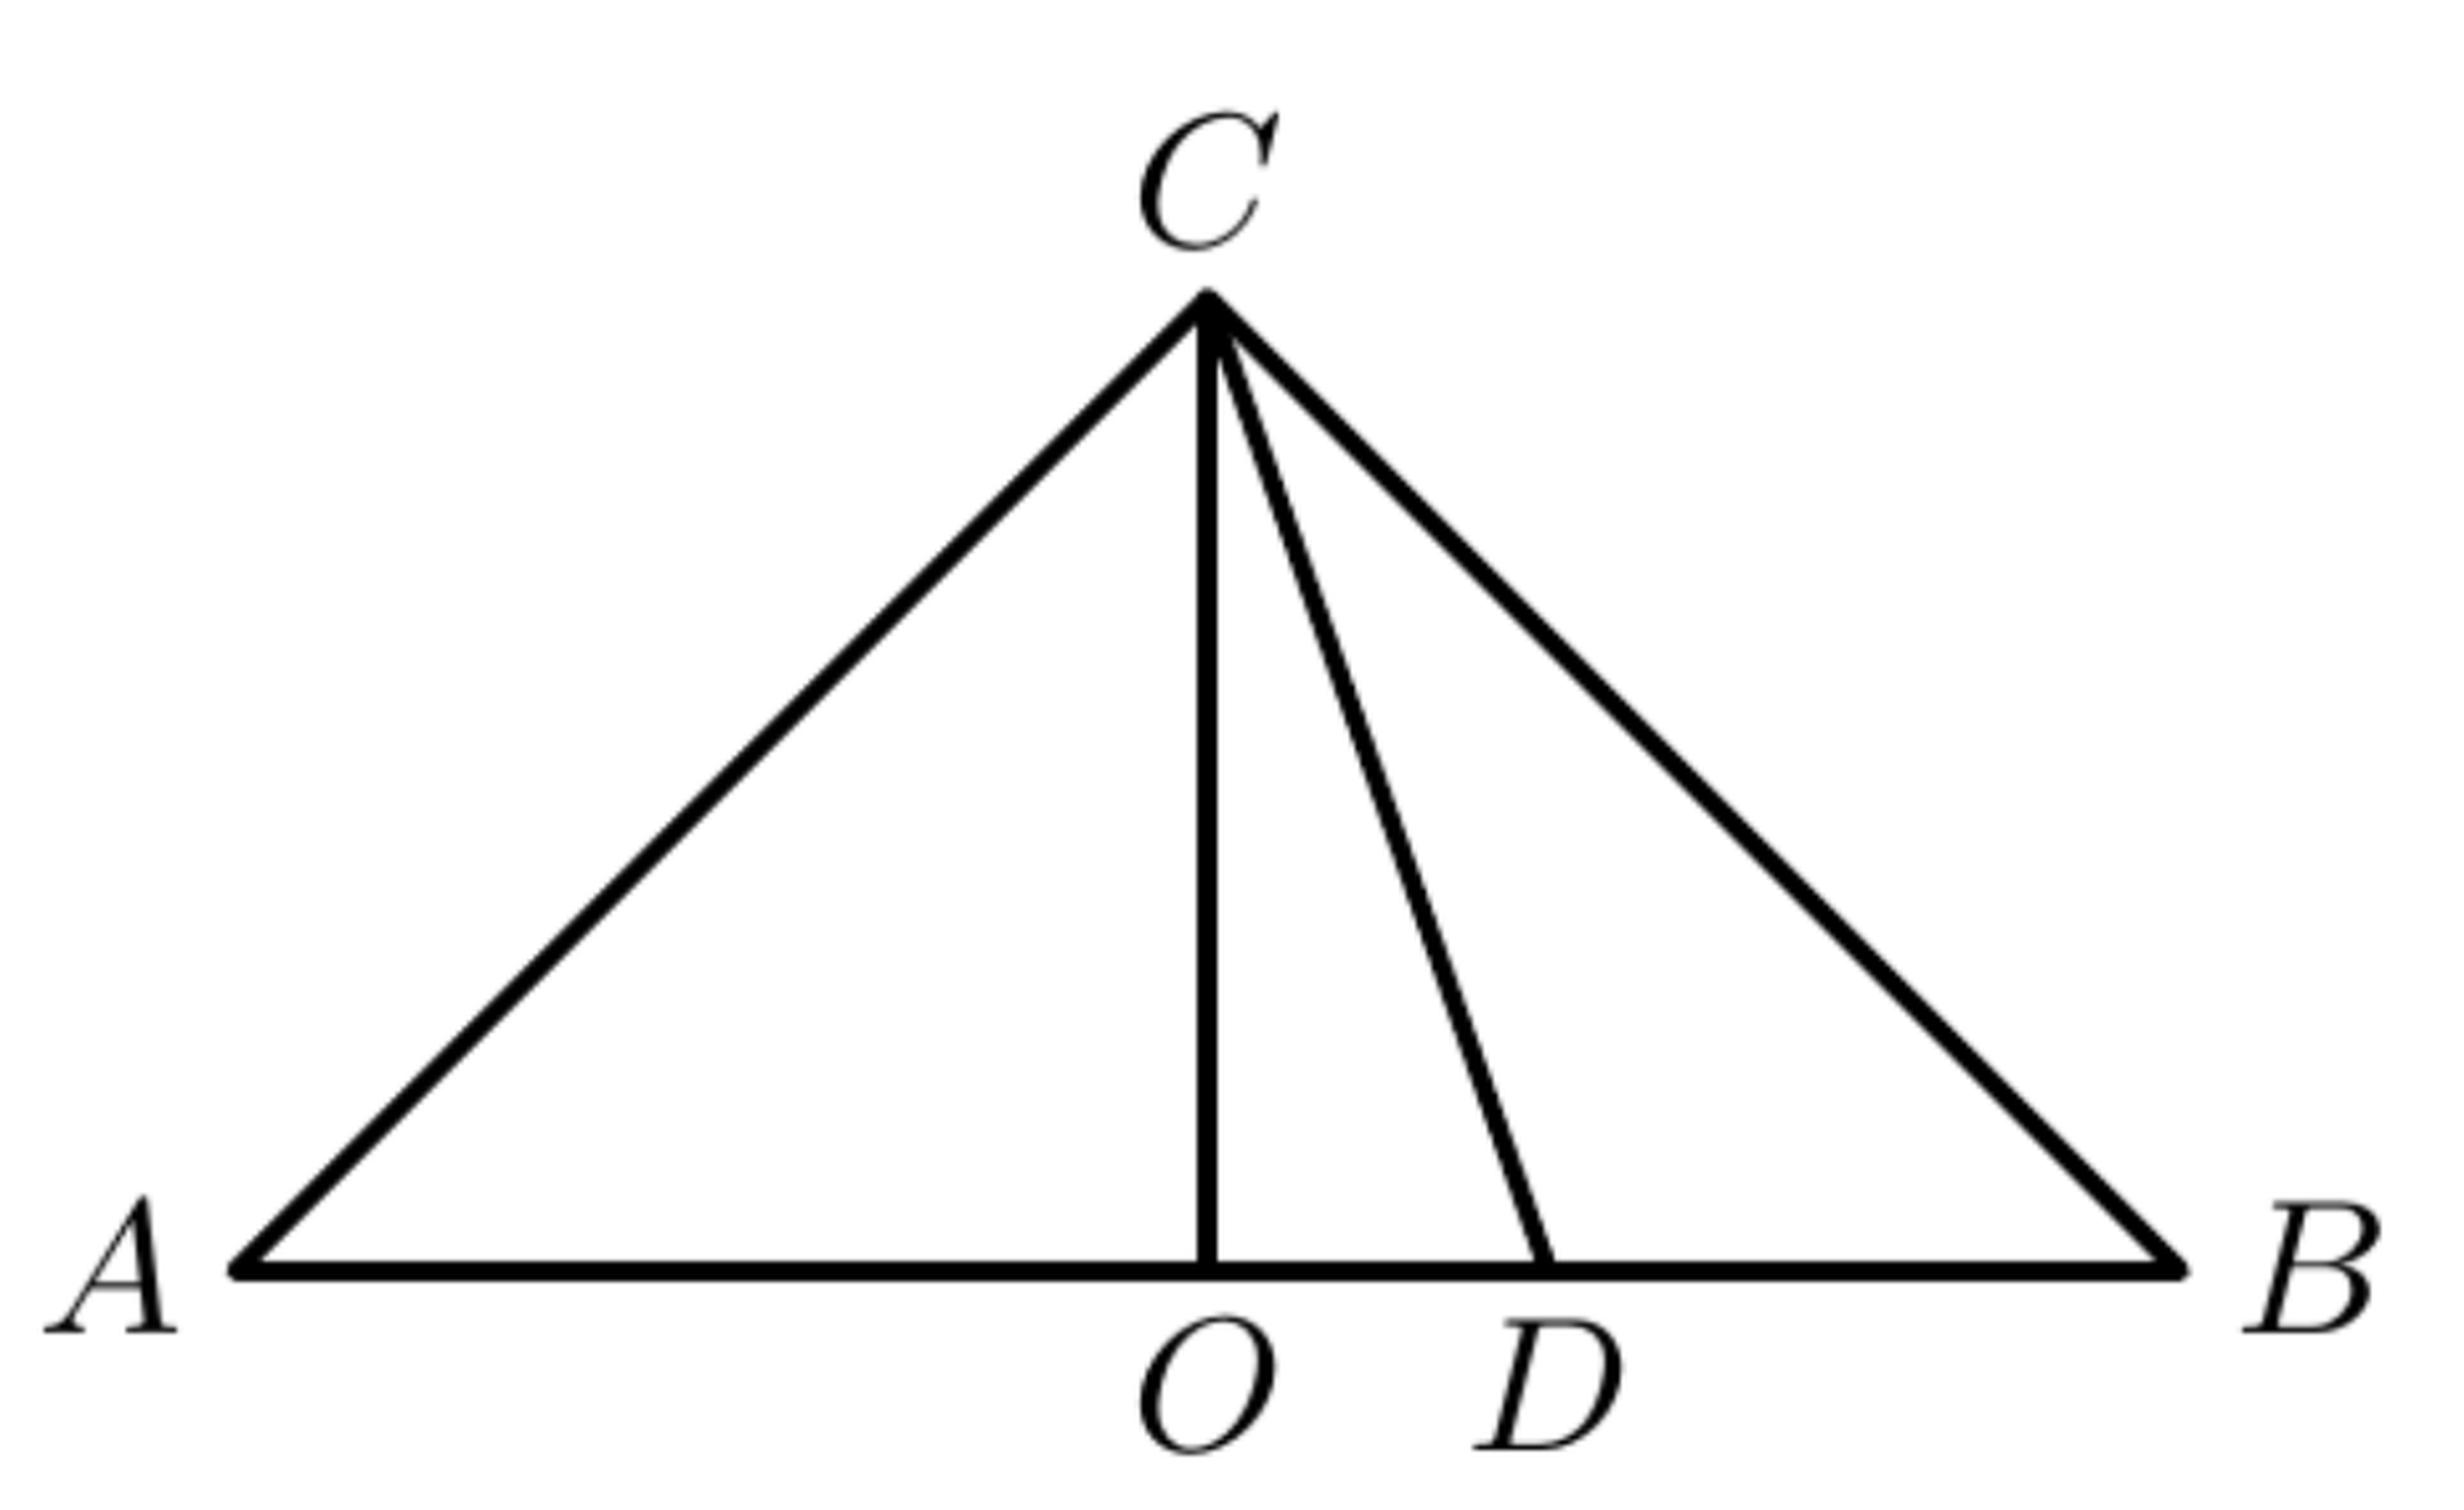
\includegraphics[width=0.34\textwidth]{figures/gao160_q16.png}
\end{center}

\keepwithprev
A. $\dfrac{a+b}{2}\geqslant\sqrt{ab}$ ($a>0,b>0$)\qquad B. $a^2+b^2\geqslant2\sqrt{ab}$ ($a>0,b>0$)

C. $\dfrac{a+b}{2}\leqslant\sqrt{\dfrac{a^2+b^2}{2}}$ ($a>0,b>0$)\qquad D. $\dfrac{2ab}{a+b}\leqslant\sqrt{ab}$ ($a>0,b>0$)

\ifanswer
\solbegin
\step{$CO=AO=\dfrac{a+b}{2},OD=\left\lvert a-\dfrac{a+b}{2}\right\rvert=\dfrac{\lvert a-b\rvert}{2}$，}
\step{$CD=\sqrt{CO^2+OD^2}=\sqrt{\dfrac{a^2+b^2}{2}}\geqslant CO=\dfrac{a+b}{2}$，}
\step{等号当且仅当 $a=b$ 时成立，故选 $C$.}
\solend
\fi

\end{enumerate}

\bigsec{三、解答题}

\begin{enumerate}
\setcounter{enumi}{16}

% === Q17 === cases 块算一行；判别式印等腰偏高三角 \Delta；解析 7 行
\item 已知幂函数 $f(x)=(m^2-2m-2)x^{m-1}$ 在 $(0,+\infty)$ 上是严格增函数.

(1) 求 $m$ 的值；

(2) 若关于 $x$ 的方程 $f(x)=(t+1)x-t^2$ 有两个不相等的正实根，求实数 $t$ 的取值范围.

\ifanswer
\solbegin
\step{(1) 幂函数的系数为 1，因此 $m^2-2m-2=1\Leftrightarrow(m-3)(m+1)=0$，}
\step{解得 $m=3$ 或 $m=-1$.}
\step{由 $f(x)$ 在 $(0,+\infty)$ 上严格递增，得 $m-1>0$，所以 $m=3$，}
\step{此时 $f(x)=x^2$.}
\step{(2) 原方程化为 $x^2-(t+1)x+t^2=0$，}
\step{方程有两个不相等的正实根，则 $\begin{cases}\Delta=(t+1)^2-4t^2=(1-t)(3t+1)>0\\t+1>0\\t^2>0\end{cases}$，}% 判别式原卷印等腰偏高三角 \Delta，照录
\step{得 $t\in\left(-\dfrac{1}{3},0\right)\cup(0,1)$.}
\solend
\fi

% === Q18 === 补集上划线 \overline{A}、\subseteq 带下划线、\varnothing；解析 8 行
\item 已知集合 $A=\{x\mid\lvert x-a\rvert<a-3\}$，$B=\left\{x\mid\dfrac{x+1}{x-2}\geqslant2\right\}$.

(1) 若 $a=5$，求 $\overline{A}\cap B$；

(2) 若 $A\cap B=A$，求实数 $a$ 的取值范围.

\ifanswer
\solbegin
\step{(1) $\dfrac{x+1}{x-2}\geqslant2\Leftrightarrow\dfrac{5-x}{x-2}\geqslant0\Leftrightarrow2<x\leqslant5,B=(2,5]$，}
\step{当 $a=5$ 时，$A=\{x\mid\lvert x-5\rvert<2\}=(3,7)$，于是 $\overline{A}=(-\infty,3]\cup[7,+\infty)$，}
\step{因此 $\overline{A}\cap B=(2,3]$.}
\step{(2) $A\cap B=A$ 等价于 $A\subseteq B$.}
\step{当 $a\leqslant3$ 时，$a-3\leqslant0$，$A=\varnothing$，满足条件.}
\step{当 $a>3$ 时，$\lvert x-a\rvert<a-3\Leftrightarrow3<x<2a-3,A=(3,2a-3)$，}
\step{此时 $A\subseteq B=(2,5]$ 等价于 $2a-3\leqslant5$，即 $a\leqslant4$，结合 $a>3$ 得 $3<a\leqslant4$.}
\step{合并两种情形，实数 $a$ 的取值范围为 $(-\infty,4]$.}
\solend
\fi

% === Q19 === 数据表 tabular 重排（高一130 成例）；cases 块算一行；解析 6 行
\item 作为我国最高水平的综合性运动会，全运会汇聚了国内顶尖体育健儿，某代表队从第 8 届全运会开始登上赛场，且参赛运动员人数逐年递增. 设 $t$ 为该代表队参赛后经过的届数，即第 8 届为 $t=0$，第 9 届为 $t=1$，以此类推. 经过 $t$ 届，运动员人数为 $y$ 人，具体数据如下：

\begin{center}
\begin{tabular}{cccccc}
$t$ & 0 & 1 & 2 & 3 & 4 \\
\hline
届数 & 8 & 9 & 10 & 11 & 12 \\
运动员人数（$y$ 人） & 4 & 11 & 25 & 53 & 109
\end{tabular}
\end{center}

(1) 现有以下两种函数模型：① $y=a\cdot b^t+c$ ($a>0,b>1$)；② $y=\log_a(t+b)+c$ ($b>0,a>1$). 请根据上表中运动员人数的增长规律，选出你认为符合的函数模型（不用说明理由），并利用表中前 3 组数据求出相应的函数解析式；

(2) 若参赛运动员人数按照 (1) 中求得的模型继续增长，在第几届全运会时，该代表队运动员人数将会首次超过 1000 人？

\ifanswer
\solbegin
\step{(1) 选模型①，将前 3 组数据代入，得 $\begin{cases}a+c=4\\ab+c=11\\ab^2+c=25\end{cases}$，}% 原卷印"选模型①"（圈数字①），OCR 误作"四"，照录①，见头注 ⑤ 3
\step{相邻两式相减，得 $a(b-1)=7$，$ab(b-1)=14$，}
\step{两式相除得 $b=2$，进而 $a=7$，$c=-3$，所求函数解析式为 $y=7\cdot2^t-3$.}
\step{(2) $y=7\cdot2^t-3$ 随 $t$ 的增大而增大，且 $t=7$ 时，$y=893<1000$；}
\step{$t=8$ 时，$y=1789>1000$，}
\step{$t$ 为非负整数，首次超过 1000 人时 $t=8$，对应第 $8+8=16$ 届全运会.}
\solend
\fi

% === Q20 === 解析 12 行（跨 08—09 页）
\item 已知函数 $f(x)=\log_a(a-a^x)$.

(1) 求该函数的定义域；

(2) 若 $a>1$，试判断关于 $x$ 的方程 $f(x)=2$ 是否有实数解，并说明理由；

(3) 若当 $x\in(-\infty,0]$ 时，关于 $x$ 的不等式 $f(x)\geqslant-1$ 恒成立，求实数 $a$ 的取值范围.

\ifanswer
\solbegin
\step{(1) 对数的底数须满足 $a>0$ 且 $a\ne1$，真数须满足 $a-a^x>0$，即 $a^x<a^1$.}% 原卷印 $a^1$，照录未化简，见头注 ⑤ 4
\step{当 $a>1$ 时，$x<1$，定义域为 $(-\infty,1)$.}
\step{当 $0<a<1$ 时，$x>1$，定义域为 $(1,+\infty)$.}
\step{(2) 当 $a>1$ 时，若 $f(x)=2$，则 $a-a^x=a^2\Rightarrow a^x=a(1-a)<0$，}
\step{这与 $a^x>0$ 矛盾，因此方程无实数解.}
\step{(3) 不等式在 $(-\infty,0]$ 上恒成立，须先保证该区间包含于函数的定义域，}
\step{由 (1) 得 $a>1$.}
\step{当 $x\leqslant0$ 时，$0<a^x\leqslant1$，所以 $a-a^x\geqslant a-1>0$.}
\step{由对数函数的单调性，$f(x)=\log_a(a-a^x)\geqslant\log_a(a-1)=f(0)$，}
\step{等号当且仅当 $x=0$ 时成立，}
\step{因此所求条件等价于 $\log_a(a-1)\geqslant-1\Leftrightarrow a-1\geqslant\dfrac{1}{a}\Leftrightarrow a^2-a-1\geqslant0$，}
\step{结合 $a>1$，得 $a\in\left[\dfrac{1+\sqrt{5}}{2},+\infty\right)$.}
\solend
\fi

% === Q21 === "和积平衡集"定义证明题；\N；解析 18 行（跨 09—10 页）
\item 已知有限集 $A=\{a_1,a_2,\cdots,a_n\}$ ($n\geqslant2,n\in\N$)，如果 $A$ 中元素 $a_i$ ($i=1,2,3,\cdots,n$) 满足 $a_1+a_2+a_3+\cdots+a_n=a_1\times a_2\times\cdots\times a_n$，就称 $A$ 为“和积平衡集”.

(1) 分别判断集合 $A=\{1,2,3,4\}$，$B=\{4+2\sqrt{2},4-2\sqrt{2}\}$ 是否为“和积平衡集”；

(2) 已知 $a_1$、$a_2$ 是两个不同的正数，且 $\{a_1,a_2\}$ 是“和积平衡集”，请用反证法证明：$a_1$、$a_2$ 至少有一个大于 2；

(3) 若 $a_i\geqslant1$，且 $a_i\in\N$，求所有符合条件的“和积平衡集”.

\ifanswer
\solbegin
\step{(1) 因为 $1+2+3+4=10\ne24=1\times2\times3\times4$，所以 $A$ 不是“和积平衡集”.}
\step{因为 $(4+2\sqrt{2})+(4-2\sqrt{2})=8=(4+2\sqrt{2})(4-2\sqrt{2})$，}
\step{所以 $B$ 是“和积平衡集”.}
\step{(2) 假设 $a_1$、$a_2$ 都不大于 2，则 $\dfrac{1}{a_1}\geqslant\dfrac{1}{2},\dfrac{1}{a_2}\geqslant\dfrac{1}{2}$，}
\step{由于 $a_1\ne a_2$，上述两个不等式至少有一个严格成立.}
\step{而 $a_1+a_2=a_1a_2$，两边除以 $a_1a_2>0$，得 $1=\dfrac{1}{a_1}+\dfrac{1}{a_2}>\dfrac{1}{2}+\dfrac{1}{2}=1$，矛盾，}
\step{所以 $a_1$、$a_2$ 至少有一个大于 2.}
\step{(3) 不妨设 $a_1<a_2<\cdots<a_n$，由各元素均为正整数，得 $a_i\geqslant i$.}
\step{若 $n\geqslant4$，因其余因子均不小于 1，}
\step{有 $a_1a_2\cdots a_n\geqslant a_2a_{n-1}a_n\geqslant2(n-1)a_n>na_n>a_1+a_2+\cdots+a_n$，}
\step{与和积平衡条件矛盾，因此只需讨论 $n=2,3$.}
\step{当 $n=2$ 时，$a_1+a_2=a_1a_2\Leftrightarrow(a_1-1)(a_2-1)=1$，}
\step{两个因子均为非负整数，只能有 $a_1=a_2=2$，与元素互不相同矛盾.}
\step{当 $n=3$ 时，若 $a_1\geqslant2$，则 $a_2\geqslant3$，从而 $a_1a_2a_3\geqslant6a_3>3a_3>a_1+a_2+a_3$，}
\step{矛盾，因此 $a_1=1$.}
\step{此时 $1+a_2+a_3=a_2a_3\Leftrightarrow(a_2-1)(a_3-1)=2$，}
\step{由 $1\leqslant a_2-1<a_3-1$，得 $a_2-1=1$、$a_3-1=2$，即 $a_2=2$、$a_3=3$.}
\step{检验 $1+2+3=1\times2\times3=6$，所求集合为 $\{1,2,3\}$.}
\solend
\fi

\end{enumerate}

\end{document}
"
% 紧凑版：xelatex "\def\iscompact{1}% 高一160_奉贤中学_期中.tex
%   —— 高一上数学"2026-2027 年奉贤中学高一上期中"（试卷版/答案版/紧凑版）
% 试卷版：xelatex 高一160_奉贤中学_期中.tex
% 答案版：xelatex "\def\isanswer{1}% 高一160_奉贤中学_期中.tex
%   —— 高一上数学"2026-2027 年奉贤中学高一上期中"（试卷版/答案版/紧凑版）
% 试卷版：xelatex 高一160_奉贤中学_期中.tex
% 答案版：xelatex "\def\isanswer{1}\input{高一160_奉贤中学_期中.tex}"
% 紧凑版：xelatex "\def\iscompact{1}\input{高一160_奉贤中学_期中.tex}"
%
% ① 原始材料：微信公众号"魔都数学加油站"文章，连载"27学年高一160"，原卷卷面标题
% "2026-2027 年奉贤中学高一上期中"（卷面未印副标题、未印连载号）。
% 正文为 10 张 PNG 页（01/04/10 为 2560×3620，02/03/05/06/07/08/09 为
% 4762×6735，同一篇各页分辨率混排，逐页按各自分辨率裁图核对）。
% 体例：讲评版——填空 3—12（10 题）、选择 13—16（4 题）、解答 17—21（5 题），
% 共 19 题，自第 3 题起编（1、2 未印在本篇）；19 题逐题印【解析】，无只印【答案】
% 的题；四道选择题答案在解析末句"故选 $B$/$B$/$D$/$C$"，题干括号
% \mbox{（\quad）} 留空、不另提 \ans{}。题目、答案、解析均据原图转录；卷面粉红色
% 水印"魔都数学加油站"及公众号页脚未录入。
% 全卷插图清单（逐页通读 10 页确认）：2 幅，均为题目配图、三版都出——
%   · Q4 韦恩图（01 页右侧：矩形全集 U、两圆 A/B、阴影部分 B∩上划线 A、
%     标注 U/A/B），裁 figures/gao160_q4.png；
%   · Q16 等腰直角三角形 ABC 图（05 页右下：C 顶点、A/O/D/B 共线底边、
%     CO 与 CD 两条线段），裁 figures/gao160_q16.png；
%   两图均取原卷截图 3—4× LANCZOS 放大、去粉色水印、转灰度、autocontrast；
%   Q4 图左侧题干残字"示"、Q16 图左侧题干残字均已裁白。
%   Q19 有一张 3 行数据表（t／届数／运动员人数（y 人），t=0..4），按全稿
%   成例（高一130）用 tabular 重排，不做成 png；其余各页无题目配图、
%   无解析内配图、无其它表格、无"如图"处。
%
% 卷首标题：原卷印作"2026-2027 年奉贤中学高一上期中"，年份区间按全稿惯例排 en dash；
% 原卷卷面未印副标题，本稿按同期中卷知识模块口径补出"集合与常用逻辑用语、不等式、函数"。
%
% ② 与原卷的排版差异／照录项清单：
%   ① 原文从第 3 题起，本稿保留原题号；共 19 题三节，解答题 5 题到 21；
%      三节各自一个 enumerate + \setcounter{enumi}{2}/{12}/{16}（不贯穿），
%      用 \examtitlest[3] 起手；
%   ② 混合体例说明：19 题全印【解析】、用 \solbegin…\solend，无只印【答案】
%      或答案印括号内的题；四道选择题答案在解析末句"故选 $B$/$B$/$D$/$C$"
%      （逐个放大复核）、括号 \mbox{（\quad）} 留空、不另提 \ans{}；答案版
%      【答案】/【解析】标记数 = 19 = 全卷题数（0 个 \ans ＋ 19 个 \solbegin）；
%   ③ 原卷卷面未印副标题，本稿按知识模块口径补出；
%   ④ 原卷填空横线按全稿惯例排 \blankline[4.4em]；选择题括号排 \mbox{（\quad）}、
%      四道选择题的选项段前按惯例各加 \keepwithprev；解答题不留作答区、不加
%      \anspace（原卷为讲评版，109—113 起全稿不用 \anspace）；
%   ⑤ 数集归一：Q4"$U=\Z$"、Q9"$a\in\R$，$b\in\R$"、Q11"$n\in\Z$"、
%      Q15"$s\in\R$"、Q21"$n\in\N$""$a_i\in\N$"原卷印正体粗体 Z/R/N，
%      按全稿惯例归一 \Z／\R／\N；集合描述竖线排 \mid（Q3、Q4、Q12、
%      Q18、Q21）；空集 \varnothing（Q18 解析 (2)）；补集照原卷上划线排
%      \overline{A}（Q4 解析、Q18 (1) 题干与解析）；子集符号 Q18 两处
%      "$A\subseteq B$"印带下划线 ⊆、照录 \subseteq；
%   ⑥ 绝对值排 \lvert…\rvert（Q7、Q8 题干与解析、Q9 题干、Q16 解析、
%      Q18 题干与解析），Q16 解析的 \left\lvert…\right\rvert 与 \lvert…\rvert
%      均在同一 $…$ 组内配对平衡；
%   ⑦ 判别式两形混用逐处照录不统一（放大逐处确认）：Q3 解析
%      "$\triangle=1^2-4a\times\frac{1}{4}=0$"原卷印扁等边三角、照录
%      \triangle；Q17 解析 cases 块"$\Delta=(t+1)^2-4t^2=(1-t)(3t+1)>0$"
%      原卷印等腰偏高三角、照录 \Delta；Q16 题干几何符号"$\triangle ABC$"
%      按全稿几何三角形记号惯例归一 \triangle（参照 高一150／132 成例）；
%   ⑧ 不等号按全稿惯例排 \leqslant／\geqslant；中文弯引号照录：Q9 题干
%      "充分非必要""必要非充分""充要""既非充分又非必要"、Q14 题干
%      "存在 $x\in(1,+\infty)$，使得 $f(x)>0$"与解析"存在""对任意"、
%      Q21 题干与解析多处"和积平衡集"；注释里一律 ASCII 引号；
%   ⑨ 文本圈数字逐处照录：Q12 题干①②③、Q12 解析"故①正确""同②得"
%      "故②正确""③假设""故③错误""故真命题是①②"、Q19 题干①②与解析
%      "选模型①"，均为印刷圈数字（非 \textcircled、非数学模式）；
%   ⑩ 半角逗号在数学组之间是全稿惯例、非笔误，逐处照录（Q8"$2^t,2^{-t}$"、
%      Q9"$a=-1,b=-2$""$a=1,b=-1$"、Q11"$1\leqslant a<10,n\in\Z$"、
%      Q12"$s_1=\frac{1}{2},t_1=x_n$"、Q16 选项"$a>0,b>0$"与解析
%      "$CO=AO=\frac{a+b}{2},OD=...$"、Q18"$2<x\leqslant5,B=(2,5]$"
%      "$3<x<2a-3,A=(3,2a-3)$"、Q21"$n=2,3$"等）；行中全角逗号／顿号
%      照录（Q15 选项"$a>1$，且 $s>0$"、Q12 解析"$s$、$t$"、Q21 解析
%      "$a_1$、$a_2$"），顿号一律移出数学模式；
%   ⑪ "图像／图象"逐处照录：本卷 Q5"的图像恒过一个定点"、Q10"的图像经过点"、
%      Q13 题干两处"图像"与解析"对称图像对应的函数"均印"图像"（有亻）；
%      Q16 印"图形"（利用图形说明、该图形能说明），无"图象"用例；
%   ⑫ 复杂式照录别简化：Q3 $ax^2+x+\frac14=0$、Q5 $y=\log_a(5x-9)-4$、
%      Q6 $(1-2x)^{\frac34}>x^{\frac34}$ 与 $\left[0,\frac12\right]$、
%      Q8 $\frac{s+\sqrt{s^2-4}}{2}$、Q10 $y=\frac{2^x}{2^x+ax}$ 与
%      $\frac{2^p}{2^p+ap}=\frac56$、$\frac{2^q}{2^q+aq}=\frac16$、
%      Q11 $N=a\times10^n$ 与 $3^{2026}$、$2026\lg3\approx966.60$、
%      $966.64512<2026\lg3<966.66538$、Q12 $Y=\{(s,t)\mid s\in X,t\in X\}$
%      与 $\frac12 s+tx_n=0$、Q16 $\sqrt{\frac{a^2+b^2}{2}}$、
%      Q17 $x^2-(t+1)x+t^2=0$ 与 $\left(-\frac13,0\right)\cup(0,1)$、
%      Q18 $\frac{5-x}{x-2}\geqslant0$、Q19 $y=a\cdot b^t+c$ 与
%      $y=\log_a(t+b)+c$、$y=7\cdot2^t-3$、Q20 $f(x)=\log_a(a-a^x)$
%      与 $a^2-a-1\geqslant0$、$\left[\frac{1+\sqrt5}{2},+\infty\right)$、
%      Q21 $4+2\sqrt2$ 与 $(a_2-1)(a_3-1)=2$ 等；
%   ⑬ 子题标号 (1)(2)(3) 按全稿惯例排半角括号；行末／行中句点按全稿惯例
%      排 ASCII `.`（不是全角「．」）；cases 块整体算一个印刷行
%      （Q17 解析、Q19 解析 (1)）；
%   ⑭ 配图：Q4／Q16 题目配图（三版都出）放 \item 内题干之后 \begin{center}，
%      各用 \needvspace{8cm} 守卫把整块推走，**守卫放在 \item 之前**
%      （见 高一153 Q11/Q19 成例与切页审计 B 类坑）；
%   ⑮ 一条 \step = 原卷解析的一个印刷行；跨上下半页的重叠行只算一次
%      （Q4 解析、Q9 解析首行、Q11 解析首行、Q12 解析"若 $s=-1$…"一行、
%      Q18 解析"此时 $A\subseteq B=(2,5]$…"一行、Q20 (2) 题干、
%      Q21 解析"由 $1\leqslant a_2-1<a_3-1$…"一行）；原卷折行别合并；
%   ⑯ Q10 之后另有一整块【注】按语（03 页上半，5 个印刷行），是讲评版作者对
%      原卷数据自相矛盾的加注、不属于任何题的【解析】。本稿按 高一53
%      "注：…"成例放 Q10 的 \solend 之后、Q10 的 \fi 收尾之前：
%      **整块只保留 Q10 那一层外层 \ifanswer**（那个 \fi 就是 Q10 的收尾），
%      块内 \stepm{【注】}{首行} ＋ 4 条 \step 各自自带内层 \ifanswer…\fi
%      （\step／\stepm 宏内自带，源码里不手动再包一层 \ifanswer，
%      否则 题目溯源.py 的 strip_answers 非贪婪正则会错切）；
%      \stepm 第一参数直接用「【注】」作标签，与全稿 \ans 的【答案】、
%      \solbegin 的【解析】同性质，未加粗以外不另加任何样式；
%      5 行仅答案版出、不新增 \item、不影响溯源，头注 ③ 单列登记、
%      不计入 19 题逐题 \step 账；\stepm 把【注】排成加粗着色标签
%      （原卷为黑色加粗），此一处着色差异在此登记；
%   ⑰ 原卷用字照录：Q11"约翰·纳皮尔""莱布尼兹"（原卷作"兹"，非通行"茨"）、
%      "17 世纪的三大数学发明"；Q16"数学说明的方法""点 $D$ 为斜边 $AB$ 上
%      异于顶点的一个动点"；Q19"登上赛场""以此类推"；
%
% ③ 行数复核：一条 \step = 原卷解析的一个印刷行，cases 块作一个印刷行计。
%   逐题数（逐页核对定稿）：Q3：5；Q4：1；Q5：1；Q6：2；Q7：2；Q8：4；
%   Q9：4；Q10：3；Q11：6；Q12：19；Q13：1；Q14：2；Q15：3；Q16：3；
%   Q17：7；Q18：8；Q19：6；Q20：12；Q21：18。
%   合计 107 条 \step（19 题逐题印刷行账），与原卷逐题印刷行相等。
%   **本卷源码 \step 总数 = 19 题逐题合计 107 ＋ Q10 后独立【注】块 5 行
%   = 112 行**（其中 \step 111 条、\stepm 1 条；\stepm 与 4 条 \step 合为
%   【注】块 5 印刷行）。该 5 行不计入「逐题印刷行」账，也不是任何题的
%   【解析】，而是讲评版编者按语；主会话核验脚本按全文统计 \step 时总数会
%   较逐题账多 5，已与主会话对齐、属已知预期而非错误。
%   全卷 19 题均设 \solbegin…\solend，答案版【答案】/【解析】标记数
%   = 19 = 全卷题数。
%
% ④ 页码分布（供回原图复核）：
%   卷首标题＋"一、填空题"＋Q3 题干＋解析 5 行＋Q4 题干＋韦恩图＋解析
%   1 行＋Q5 题干首行在 01 页上半；Q4 解析（重叠）＋Q5 题干续＋解析 1 行＋
%   Q6 题干＋解析 2 行＋Q7 题干＋解析首行在 01 页下半；Q7 解析末行＋
%   Q8 题干＋解析 4 行＋Q9 题干＋解析首行在 02 页上半；Q9 解析（重叠首行）
%   ＋余 3 行＋Q10 题干＋解析 3 行在 02 页下半；【注】按语 5 行＋Q11 题干＋
%   解析首行在 03 页上半；Q11 解析（重叠首行）＋余 5 行＋Q12 题干＋①②
%   在 03 页下半；Q12 ③＋解析前 9 行在 04 页上半；Q12 解析（重叠 2 行）
%   ＋余 8 行在 04 页下半；Q12 解析末 2 行＋"二、选择题"＋Q13 题干＋选项＋
%   解析 1 行＋Q14 题干＋选项＋解析首行在 05 页上半；Q14 解析末行＋
%   Q15 题干＋选项＋解析 3 行＋Q16 题干＋三角形图在 05 页下半；
%   Q16 选项＋解析 3 行＋"三、解答题"＋Q17 题干＋两问在 06 页上半；
%   Q17 解析 7 行在 06 页下半；Q18 题干＋两问＋解析前 7 行＋Q19 题干首行
%   在 07 页上半；Q18 解析末行（重叠）＋Q19 题干＋表格＋两问在 07 页下半；
%   Q19 解析 6 行＋Q20 题干＋(1)(2) 在 08 页上半；Q20 (2)(3) 题干（重叠）
%   ＋解析 8 行在 08 页下半；Q20 解析末 4 行＋Q21 题干＋(1)(2) 在 09 页
%   上半；Q21 (3)＋解析前 7 行在 09 页下半；Q21 解析 (3) 余 10 行在 10 页
%   上半；Q21 末行（重叠）＋"检验 $1+2+3=1\times2\times3=6$，所求集合为
%   $\{1,2,3\}$."在 10 页下半（此后仅水印、无正文）。本稿按题连排，
%   不丢行、不并折行；全卷末题为第 21 题，无附加题节。
%
% ⑤ 存疑照录（放大原图确认，照录未改、正文对应处另有 % 注）：
%   1. Q10【注】按语：讲评版作者据 $a=\sqrt3$ 时 $2^q=\frac{\sqrt3}{5}q<q$
%      与 $2^n\geqslant n+1$ 推出点 $Q$ 不存在、"严格说本题无解"，并注明
%      "原卷数据疑似有误（同型常见题为 $P(p,\frac65)$、$Q(q,-\frac15)$、
%      $2^{p+q}=36pq$，得 $a=6$）"；本稿照录全块、未删未改（见 ② ⑯）。
%   2. Q12 解析 (3) 末段"若 $t=-1$，则 $\frac{1}{2}s=x_n\cdot(-1)$，
%      于是 $s=2x_n>x_n$，也矛盾，"中，等式右端与紧随的结论符号不自洽
%      （按题意应为 $\frac12 s=x_n$ 或 $-\frac12 s=x_n\cdot(-1)$），逐页
%      放大 04 页确认原卷即如此印、无漏看的负号，照录未改，建议主会话
%      回 04 页再放大复核一次；
%   3. Q19 解析 (1) 印"选模型①"（圈数字①，题干只有①②两种模型）；
%      OCR 误作"选模型四"，放大 08 页确认是①、照录①；
%   4. Q20 解析 (1)"即 $a^x<a^1$"末项原卷印 $a^1$（非 $a$），照录未化简；
%   5. Q11 题干"莱布尼兹"原卷作"兹"（非通行"茨"）、"约翰·纳皮尔"用
%      间隔号·，均照录未改；
%   6. Q9 题干"则 $p$ 是 $q$___条件"与解析"故 $p$ 是 $q$ 的充分非必要条件"
%      句式略异，均照录；
%   7. Q19 解析 (1) 用"前 3 组数据"、题干表格列到 $t=4$，照录未补。
%
\documentclass[a4paper,11pt]{article}
\usepackage{common}

\begin{document}

\examtitlest[3]{2026--2027 年奉贤中学高一上期中}{集合与常用逻辑用语、不等式、函数}

\bigsec{一、填空题}

\begin{enumerate}
\setcounter{enumi}{2}

% === Q3 === 解析 5 行；判别式印扁等边三角 \triangle
\item 若集合 $A=\{x\mid ax^2+x+\dfrac{1}{4}=0\}$ 有且仅有两个子集，则实数 $a=$\blankline[4.4em].

\ifanswer
\solbegin
\step{若集合 $A=\{x\mid ax^2+x+\dfrac{1}{4}=0\}$ 有且仅有两个子集，}
\step{所以方程 $ax^2+x+\dfrac{1}{4}=0$ 只有一个实数根，}
\step{当 $a=0$ 时，方程化为 $x+\dfrac{1}{4}=0$，解得 $x=-\dfrac{1}{4}$，符合题意，}
\step{当 $a\ne0$ 时，则 $\triangle=1^2-4a\times\dfrac{1}{4}=0$，解得 $a=1$，}% 判别式原卷印扁等边三角 \triangle，照录
\step{综上所述，实数 $a=0$ 或 1.}
\solend
\fi

% === Q4 === 题目配图（三版都出）；\needvspace 守卫放 \item 之前；补集上划线 \overline{A}；解析 1 行
\needvspace{8cm}
\item 设全集 $U=\Z$，集合 $A=\{x\mid -3<x<1\}$，$B=\{-1,0,1,2\}$，用列举法表示图中阴影部分为\blankline[4.4em].

\begin{center}
% Q4 韦恩图（全集 U、A/B 两圆、阴影 B∩上划线 A）取 01 页右侧，去粉色水印、去色、4× LANCZOS 放大；三版都出
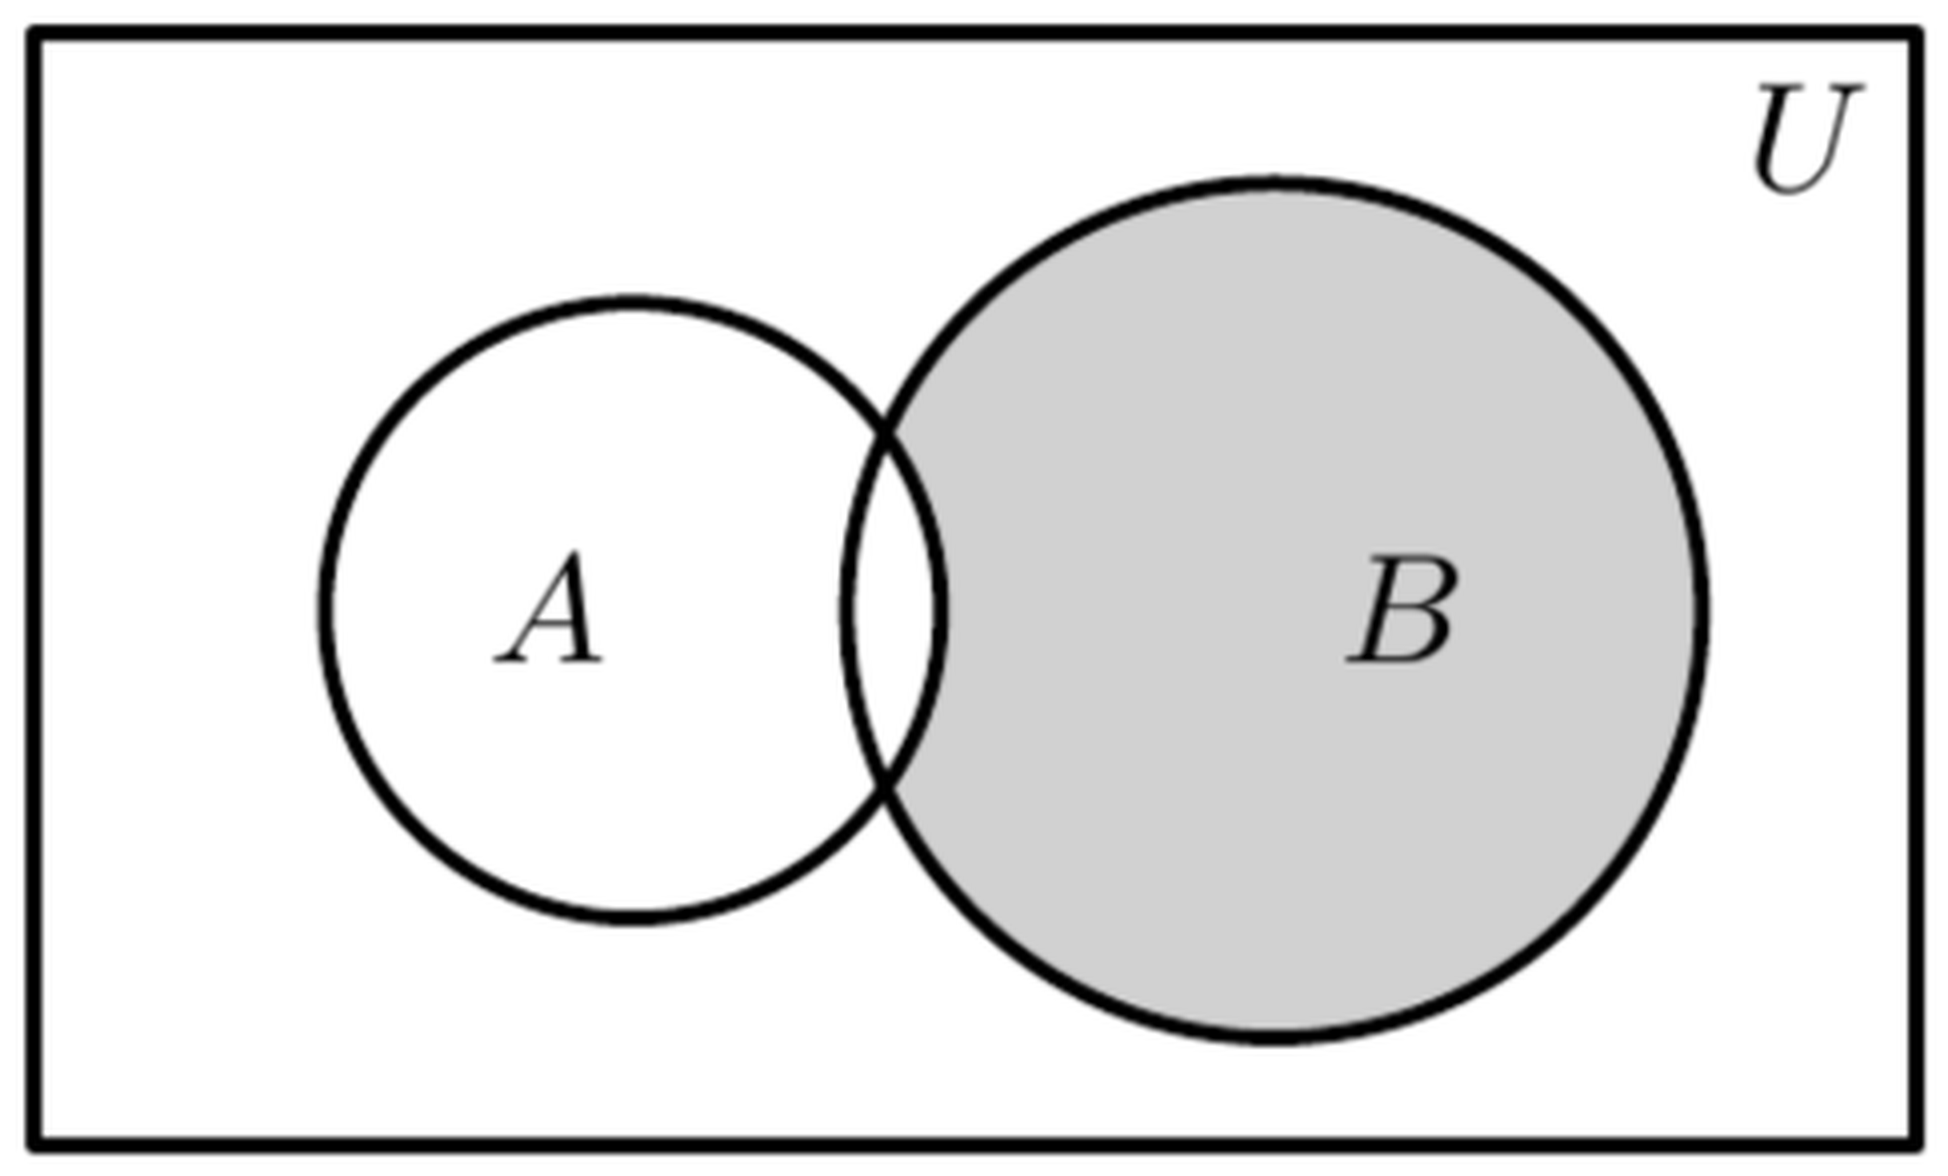
\includegraphics[width=0.38\textwidth]{figures/gao160_q4.png}
\end{center}

\ifanswer
\solbegin
\step{阴影部分表示 $B\cap\overline{A}=\{1,2\}$.}
\solend
\fi

% === Q5 === "图像"（有亻）照录；解析 1 行
\item 已知常数 $a>0$ 且 $a\ne1$，假设无论 $a$ 取何值，函数 $y=\log_a(5x-9)-4$ 的图像恒过一个定点，则这个定点的坐标为\blankline[4.4em].

\ifanswer
\solbegin
\step{$5x-9=1\Rightarrow x=2$，此时 $y=\log_a 1-4=-4$，定点为 $(2,-4)$.}
\solend
\fi

% === Q6 === 解析 2 行
\item 不等式 $(1-2x)^{\frac{3}{4}}>x^{\frac{3}{4}}$ 的解集为\blankline[4.4em].

\ifanswer
\solbegin
\step{定义域为 $\left[0,\dfrac{1}{2}\right]$，由幂函数的单调性，原不等式等价于 $1-2x>x$，}
\step{得 $0\leqslant x<\dfrac{1}{3}$，故解集为 $\left[0,\dfrac{1}{3}\right)$.}
\solend
\fi

% === Q7 === 绝对值 \lvert…\rvert；解析 2 行（跨 01—02 页）
\item 已知不等式 $\lvert x+3\rvert+\lvert x-2\rvert\geqslant 5$，当其等号成立时，$x$ 的取值范围是\blankline[4.4em].

\ifanswer
\solbegin
\step{$\lvert x+3\rvert+\lvert x-2\rvert=\lvert x+3\rvert+\lvert 2-x\rvert\geqslant\lvert(x+3)+(2-x)\rvert=5$，}
\step{等号成立当且仅当 $(x+3)(2-x)\geqslant0$，即 $x\in[-3,2]$.}
\solend
\fi

% === Q8 === 解析 4 行
\item 已知函数 $f(x)=\lvert\log_2 x\rvert$，若方程 $f(x)-t=0$ 有两个不同的实数根 $x_1,x_2$，则 $x_1+x_2$ 的取值范围是\blankline[4.4em].

\ifanswer
\solbegin
\step{方程有两个不同实根，必有 $t>0$，两根为 $2^t,2^{-t}$，}
\step{所以 $x_1+x_2=2^t+2^{-t}>2$（等号仅在 $t=0$ 时成立）.}
\step{任取 $s>2$，令 $a=\dfrac{s+\sqrt{s^2-4}}{2}>1$，取 $t=\log_2 a>0$，则 $x_1+x_2=a+\dfrac{1}{a}=s$，}
\step{所以取值范围为 $(2,+\infty)$.}
\solend
\fi

% === Q9 === 中文弯引号、\R、绝对值 \lvert…\rvert；解析 4 行
\item 已知 $a\in\R$，$b\in\R$，$p:\dfrac{1}{\lvert a\rvert}>\dfrac{1}{\lvert b\rvert}$，$q:\dfrac{1}{a}>\dfrac{1}{b}$，则 $p$ 是 $q$\blankline[4.4em]条件（用“充分非必要”、“必要非充分”、“充要”或“既非充分又非必要”填空）.

\ifanswer
\solbegin
\step{由 $p$、$q$ 中的分式有意义，$a\ne0$ 且 $b\ne0$.}
\step{当 $a=-1,b=-2$ 时，$p$ 成立而 $q$ 不成立，故 $p$ 不是 $q$ 的充分条件.}
\step{当 $a=1,b=-1$ 时，$q$ 成立而 $p$ 不成立，故 $p$ 不是 $q$ 的必要条件.}
\step{故 $p$ 是 $q$ 的充分非必要条件.}
\solend
\fi

% === Q10 === 解析 3 行；其后独立【注】按语 5 行（见头注 ② ⑯、⑤ 1）
\item 已知常数 $a>0$，函数 $y=\dfrac{2^x}{2^x+ax}$ 的图像经过点 $P\left(p,\dfrac{5}{6}\right)$、$Q\left(q,\dfrac{1}{6}\right)$，若 $2^{p+q}=3pq$，则 $a=$\blankline[4.4em].

\ifanswer
\solbegin
\step{由 $\dfrac{2^p}{2^p+ap}=\dfrac{5}{6}$ 得 $2^p=5ap$；由 $\dfrac{2^q}{2^q+aq}=\dfrac{1}{6}$ 得 $2^q=\dfrac{aq}{5}$.}
\step{$2^p>0$，$2^q>0$，$a>0$，得 $p>0$，$q>0$.}
\step{两式相乘得 $2^{p+q}=a^2pq$，又 $2^{p+q}=3pq$ 且 $pq\ne0$，故 $a^2=3$，$a=\sqrt{3}$.}
\solend
% 【注】按语（讲评版编者按，5 个印刷行，仅答案版出，不属于任何题的【解析】）
\stepm{【注】}{按原卷数据严格推敲，点 $Q$ 其实不存在：$a=\sqrt{3}$ 时 $2^q=\dfrac{\sqrt{3}}{5}q<q$；而当 $q>0$}
\step{时，取非负整数 $n$ 使 $n\leqslant q<n+1$，由 $2^{k+1}=2^k+2^k\geqslant2^k+1$ 逐次推得 $2^n\geqslant n+1$，于是}
\step{$2^q\geqslant2^n\geqslant n+1>q$，矛盾. 所以题设条件互相矛盾，严格说本题无解；$\sqrt{3}$ 是由题给关}
\step{系直接推出的值，按命题意图作为答案. 原卷数据疑似有误（同型常见题为 $P\left(p,\dfrac{6}{5}\right)$、}
\step{$Q\left(q,-\dfrac{1}{5}\right)$、$2^{p+q}=36pq$，得 $a=6$）.}% 见头注 ⑤ 1，照录未改
\fi

% === Q11 === 纳皮尔对数材料题；\Z、大数；解析 6 行
\item 17 世纪初，约翰·纳皮尔为了简化计算而发明了对数. 对数的发明是数学史上的重大事件，恩格斯曾经把笛卡尔的坐标系、纳皮尔的对数、牛顿和莱布尼兹的微积分共同称为 17 世纪的三大数学发明. 我们知道，任何一个正实数 $N$ 可以表示成 $N=a\times10^n$ ($1\leqslant a<10,n\in\Z$) 的形式，这便是科学记数法，若两边取常用对数，有 $\lg N=n+\lg a$，则可以估计 $3^{2026}$ 的最高位上的数值为\blankline[4.4em].

\ifanswer
\solbegin
\step{设 $3^{2026}=a\times10^n$ ($1\leqslant a<10,n\in\Z$)，则 $2026\lg 3=n+\lg a$.}
\step{用 $\lg 3\approx 0.4771$ 粗估，得 $2026\lg 3\approx 966.60$.}
\step{为核验误差，用 $0.47712<\lg 3<0.47713$，}
\step{得 $966.64512<2026\lg 3<966.66538$，因此 $n=966$.}
\step{于是 $\lg 4\approx 0.60206<0.64512<\lg a<0.66538<\lg 5\approx 0.69897$，}
\step{所以 $4<a<5$，最高位为 4，估算误差不影响结论.}
\solend
\fi

% === Q12 === 自定义"性质 P"；文本圈数字①②③；解析 19 行（跨 03—05 页）
\item 对于数集 $X=\{-1,x_1,x_2,x_3,\cdots,x_n\}$，其中 $0<x_1<x_2<x_3<\cdots<x_n$，$n\geqslant2$，定义点集 $Y=\{(s,t)\mid s\in X,t\in X\}$，若对于任意 $(s_1,t_1)\in Y$，存在 $(s_2,t_2)\in Y$，使得 $s_1s_2+t_1t_2=0$，则称集合 $X$ 具有性质 $P$. 则下列命题中为真命题的是\blankline[4.4em].

① $X=\{-1,1,2\}$ 具有性质 $P$；②若集合 $X$ 具有性质 $P$，则 $1\in X$；

③集合 $X$ 具有性质 $P$，若 $x_1=\dfrac{1}{2}$，则 $x_n=2$.

\ifanswer
\solbegin
\step{因为 $X=\{-1,1,2\}$，}
\step{所以 $Y=\{(-1,-1),(1,1),(2,2),(-1,1),(-1,2),(1,-1),(1,2),(2,-1),(2,1)\}$，}
\step{由集合 $X$ 具有性质 $P$ 的定义，对于任意 $(s,t)\in Y$，}
\step{若 $s>0$，$t>0$，则 $s=t$ 或 $(s,t)=(1,2)$ 或 $(s,t)=(2,1)$，}
\step{若 $s=t$，取 $s_2=-1$，$t_2=-1$，则 $ss_2+tt_2=0$；}
\step{若 $(s,t)=(1,2)$，取 $s_2=2$，$t_2=-1$，则 $ss_2+tt_2=0$；}
\step{若 $(s,t)=(2,1)$，取 $s_2=-1$，$t_2=2$，则 $ss_2+tt_2=0$；}
\step{若 $s$、$t$ 有一个为负数，则 $s=-1$ 或 $t=-1$，}
\step{若 $s=-1$，则取 $s_2=t$，$t_2=1$，则 $ss_2+tt_2=0$；}
\step{若 $t=-1$，则取 $s_2=1$，$t_2=s$，则 $ss_2+tt_2=0$；故①正确；}
\step{对于任意 $(s_1,t_1)\in Y$，存在 $(s_2,t_2)\in Y$，使得 $s_1s_2+t_1t_2=0$，}
\step{取 $(x_1,x_1)\in Y$，存在 $(x_p,x_q)$ 使得 $x_1x_p+x_1x_q=0$，所以 $x_p+x_q=0$，}
\step{不妨设 $x_p=1$，$x_q=-1$，所以若集合 $X$ 具有性质 $P$，则 $1\in X$，故②正确；}
\step{③假设 $x_n>1$，令 $s_1=\dfrac{1}{2},t_1=x_n$，则存在 $s$、$t\in X$ 使得 $\dfrac{1}{2}s+tx_n=0$，}
\step{同②得 $s$、$t$ 中必有一个数为 $-1$，}
\step{若 $s=-1$，则 $tx_n=\dfrac{1}{2}$，于是 $t=\dfrac{1}{2x_n}<\dfrac{1}{2}=x_1$，矛盾，}
\step{若 $t=-1$，则 $\dfrac{1}{2}s=x_n\cdot(-1)$，于是 $s=2x_n>x_n$，也矛盾，}% 原卷如此（与结论符号不自洽），照录未改，见头注 ⑤ 2
\step{所以 $x_n\leqslant1$，又由②得 $1\in X$，所以 $x_n\geqslant1$，所以 $x_n=1$，故③错误，}
\step{故真命题是①②.}
\solend
\fi

\end{enumerate}

% 答案版里填空解析把页排满，节标题会落到页末、与第 13 题分家（切页审计 B 类）；
% 守卫放 \bigsec 之前，连节标题一起量页高（高一157 成例）
\needvspace{7cm}
\bigsec{二、选择题}

\begin{enumerate}
\setcounter{enumi}{12}

% === Q13 === "图像"照录；解析 1 行，故选 $B$
\item 下列函数中，图像与函数 $y=3^x$ 图像关于 $y$ 轴对称的是\mbox{（\quad）}

\keepwithprev
A. $y=x^3$\qquad B. $y=\left(\dfrac{1}{3}\right)^x$\qquad C. $y=-3^x$\qquad D. $y=\log_3 x$

\ifanswer
\solbegin
\step{将 $x$ 换为 $-x$，得对称图像对应的函数为 $y=3^{-x}=\left(\dfrac{1}{3}\right)^x$，故选 $B$.}
\solend
\fi

% === Q14 === 中文弯引号；解析 2 行（跨 05 页上下），故选 $B$
\item 命题“存在 $x\in(1,+\infty)$，使得 $f(x)>0$”的否定形式为\mbox{（\quad）}

\keepwithprev
A. 不存在 $x\in(-\infty,1]$，使得 $f(x)>0$\qquad B. 对任意 $x\in(1,+\infty)$，有 $f(x)\leqslant0$

C. 对任意 $x\in(-\infty,1]$，有 $f(x)\leqslant0$\qquad D. 存在 $x\in(1,+\infty)$，使得 $f(x)\leqslant0$

\ifanswer
\solbegin
\step{将“存在”改为“对任意”，$x$ 的范围不变，并将 $f(x)>0$ 否定为 $f(x)\leqslant0$，}
\step{故选 $B$.}
\solend
\fi

% === Q15 === \R；四选项两行；解析 3 行，故选 $D$
\item 设 $a>0$，$s\in\R$. 下列各项中，能推出 $a^s>a$ 的一项是\mbox{（\quad）}

\keepwithprev
A. $a>1$，且 $s>0$\qquad B. $a>1$，且 $s<0$

C. $0<a<1$，且 $s>0$\qquad D. $0<a<1$，且 $s<0$

\ifanswer
\solbegin
\step{当 $a>1$ 时，$a^s>a\Leftrightarrow s>1$，A、B 均不能保证.}
\step{当 $0<a<1$ 时，$a^s>a\Leftrightarrow s<1$，C 不能保证，D 中 $s<0<1$，满足要求；}
\step{故选 $D$.}
\solend
\fi

% === Q16 === 题目配图（三版都出）；几何符号 \triangle ABC；解析 3 行，故选 $C$
\needvspace{8cm}
\item 数学说明的方法多种多样，其中利用图形说明就是一种重要方法. 如图所示，在等腰直角三角形 $\triangle ABC$ 中，点 $O$ 为斜边 $AB$ 的中点，点 $D$ 为斜边 $AB$ 上异于顶点的一个动点，设 $AD=a$，$BD=b$，则可用该图形能说明的不等式为\mbox{（\quad）}

\begin{center}
% Q16 等腰直角三角形 ABC 图（C/A/O/D/B 标注）取 05 页右下，去粉色水印、去色、3× LANCZOS 放大；三版都出
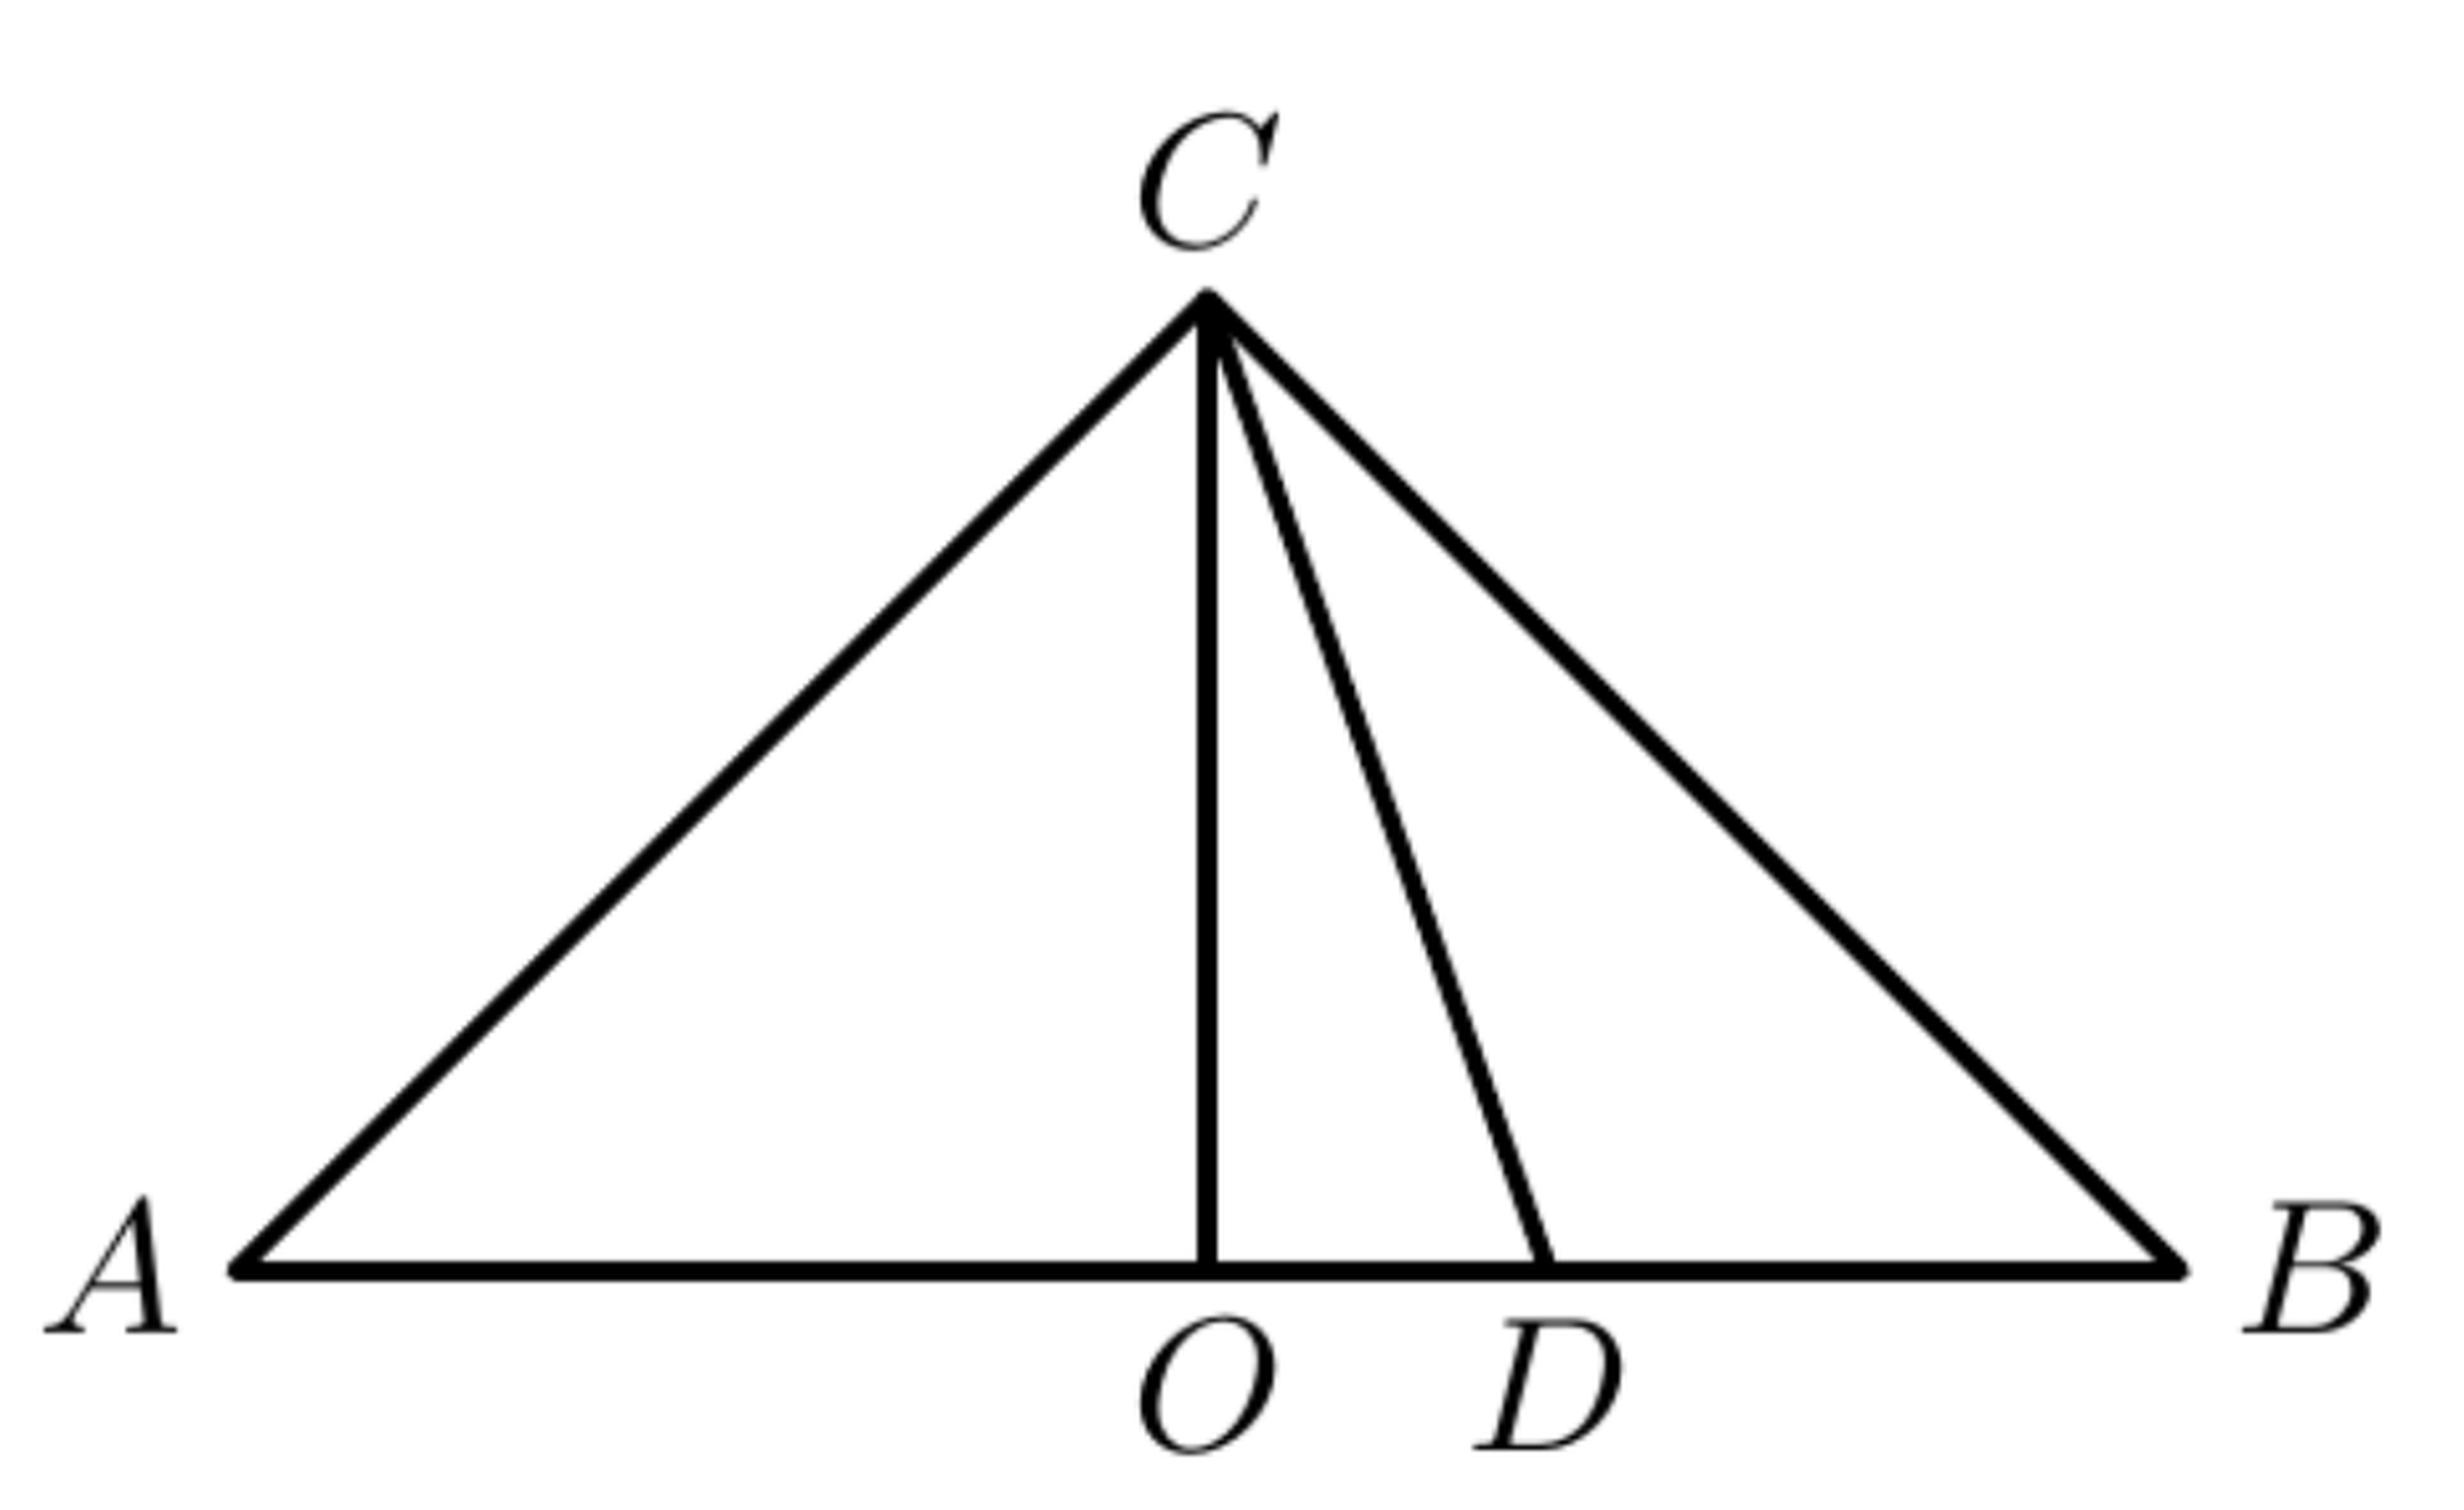
\includegraphics[width=0.34\textwidth]{figures/gao160_q16.png}
\end{center}

\keepwithprev
A. $\dfrac{a+b}{2}\geqslant\sqrt{ab}$ ($a>0,b>0$)\qquad B. $a^2+b^2\geqslant2\sqrt{ab}$ ($a>0,b>0$)

C. $\dfrac{a+b}{2}\leqslant\sqrt{\dfrac{a^2+b^2}{2}}$ ($a>0,b>0$)\qquad D. $\dfrac{2ab}{a+b}\leqslant\sqrt{ab}$ ($a>0,b>0$)

\ifanswer
\solbegin
\step{$CO=AO=\dfrac{a+b}{2},OD=\left\lvert a-\dfrac{a+b}{2}\right\rvert=\dfrac{\lvert a-b\rvert}{2}$，}
\step{$CD=\sqrt{CO^2+OD^2}=\sqrt{\dfrac{a^2+b^2}{2}}\geqslant CO=\dfrac{a+b}{2}$，}
\step{等号当且仅当 $a=b$ 时成立，故选 $C$.}
\solend
\fi

\end{enumerate}

\bigsec{三、解答题}

\begin{enumerate}
\setcounter{enumi}{16}

% === Q17 === cases 块算一行；判别式印等腰偏高三角 \Delta；解析 7 行
\item 已知幂函数 $f(x)=(m^2-2m-2)x^{m-1}$ 在 $(0,+\infty)$ 上是严格增函数.

(1) 求 $m$ 的值；

(2) 若关于 $x$ 的方程 $f(x)=(t+1)x-t^2$ 有两个不相等的正实根，求实数 $t$ 的取值范围.

\ifanswer
\solbegin
\step{(1) 幂函数的系数为 1，因此 $m^2-2m-2=1\Leftrightarrow(m-3)(m+1)=0$，}
\step{解得 $m=3$ 或 $m=-1$.}
\step{由 $f(x)$ 在 $(0,+\infty)$ 上严格递增，得 $m-1>0$，所以 $m=3$，}
\step{此时 $f(x)=x^2$.}
\step{(2) 原方程化为 $x^2-(t+1)x+t^2=0$，}
\step{方程有两个不相等的正实根，则 $\begin{cases}\Delta=(t+1)^2-4t^2=(1-t)(3t+1)>0\\t+1>0\\t^2>0\end{cases}$，}% 判别式原卷印等腰偏高三角 \Delta，照录
\step{得 $t\in\left(-\dfrac{1}{3},0\right)\cup(0,1)$.}
\solend
\fi

% === Q18 === 补集上划线 \overline{A}、\subseteq 带下划线、\varnothing；解析 8 行
\item 已知集合 $A=\{x\mid\lvert x-a\rvert<a-3\}$，$B=\left\{x\mid\dfrac{x+1}{x-2}\geqslant2\right\}$.

(1) 若 $a=5$，求 $\overline{A}\cap B$；

(2) 若 $A\cap B=A$，求实数 $a$ 的取值范围.

\ifanswer
\solbegin
\step{(1) $\dfrac{x+1}{x-2}\geqslant2\Leftrightarrow\dfrac{5-x}{x-2}\geqslant0\Leftrightarrow2<x\leqslant5,B=(2,5]$，}
\step{当 $a=5$ 时，$A=\{x\mid\lvert x-5\rvert<2\}=(3,7)$，于是 $\overline{A}=(-\infty,3]\cup[7,+\infty)$，}
\step{因此 $\overline{A}\cap B=(2,3]$.}
\step{(2) $A\cap B=A$ 等价于 $A\subseteq B$.}
\step{当 $a\leqslant3$ 时，$a-3\leqslant0$，$A=\varnothing$，满足条件.}
\step{当 $a>3$ 时，$\lvert x-a\rvert<a-3\Leftrightarrow3<x<2a-3,A=(3,2a-3)$，}
\step{此时 $A\subseteq B=(2,5]$ 等价于 $2a-3\leqslant5$，即 $a\leqslant4$，结合 $a>3$ 得 $3<a\leqslant4$.}
\step{合并两种情形，实数 $a$ 的取值范围为 $(-\infty,4]$.}
\solend
\fi

% === Q19 === 数据表 tabular 重排（高一130 成例）；cases 块算一行；解析 6 行
\item 作为我国最高水平的综合性运动会，全运会汇聚了国内顶尖体育健儿，某代表队从第 8 届全运会开始登上赛场，且参赛运动员人数逐年递增. 设 $t$ 为该代表队参赛后经过的届数，即第 8 届为 $t=0$，第 9 届为 $t=1$，以此类推. 经过 $t$ 届，运动员人数为 $y$ 人，具体数据如下：

\begin{center}
\begin{tabular}{cccccc}
$t$ & 0 & 1 & 2 & 3 & 4 \\
\hline
届数 & 8 & 9 & 10 & 11 & 12 \\
运动员人数（$y$ 人） & 4 & 11 & 25 & 53 & 109
\end{tabular}
\end{center}

(1) 现有以下两种函数模型：① $y=a\cdot b^t+c$ ($a>0,b>1$)；② $y=\log_a(t+b)+c$ ($b>0,a>1$). 请根据上表中运动员人数的增长规律，选出你认为符合的函数模型（不用说明理由），并利用表中前 3 组数据求出相应的函数解析式；

(2) 若参赛运动员人数按照 (1) 中求得的模型继续增长，在第几届全运会时，该代表队运动员人数将会首次超过 1000 人？

\ifanswer
\solbegin
\step{(1) 选模型①，将前 3 组数据代入，得 $\begin{cases}a+c=4\\ab+c=11\\ab^2+c=25\end{cases}$，}% 原卷印"选模型①"（圈数字①），OCR 误作"四"，照录①，见头注 ⑤ 3
\step{相邻两式相减，得 $a(b-1)=7$，$ab(b-1)=14$，}
\step{两式相除得 $b=2$，进而 $a=7$，$c=-3$，所求函数解析式为 $y=7\cdot2^t-3$.}
\step{(2) $y=7\cdot2^t-3$ 随 $t$ 的增大而增大，且 $t=7$ 时，$y=893<1000$；}
\step{$t=8$ 时，$y=1789>1000$，}
\step{$t$ 为非负整数，首次超过 1000 人时 $t=8$，对应第 $8+8=16$ 届全运会.}
\solend
\fi

% === Q20 === 解析 12 行（跨 08—09 页）
\item 已知函数 $f(x)=\log_a(a-a^x)$.

(1) 求该函数的定义域；

(2) 若 $a>1$，试判断关于 $x$ 的方程 $f(x)=2$ 是否有实数解，并说明理由；

(3) 若当 $x\in(-\infty,0]$ 时，关于 $x$ 的不等式 $f(x)\geqslant-1$ 恒成立，求实数 $a$ 的取值范围.

\ifanswer
\solbegin
\step{(1) 对数的底数须满足 $a>0$ 且 $a\ne1$，真数须满足 $a-a^x>0$，即 $a^x<a^1$.}% 原卷印 $a^1$，照录未化简，见头注 ⑤ 4
\step{当 $a>1$ 时，$x<1$，定义域为 $(-\infty,1)$.}
\step{当 $0<a<1$ 时，$x>1$，定义域为 $(1,+\infty)$.}
\step{(2) 当 $a>1$ 时，若 $f(x)=2$，则 $a-a^x=a^2\Rightarrow a^x=a(1-a)<0$，}
\step{这与 $a^x>0$ 矛盾，因此方程无实数解.}
\step{(3) 不等式在 $(-\infty,0]$ 上恒成立，须先保证该区间包含于函数的定义域，}
\step{由 (1) 得 $a>1$.}
\step{当 $x\leqslant0$ 时，$0<a^x\leqslant1$，所以 $a-a^x\geqslant a-1>0$.}
\step{由对数函数的单调性，$f(x)=\log_a(a-a^x)\geqslant\log_a(a-1)=f(0)$，}
\step{等号当且仅当 $x=0$ 时成立，}
\step{因此所求条件等价于 $\log_a(a-1)\geqslant-1\Leftrightarrow a-1\geqslant\dfrac{1}{a}\Leftrightarrow a^2-a-1\geqslant0$，}
\step{结合 $a>1$，得 $a\in\left[\dfrac{1+\sqrt{5}}{2},+\infty\right)$.}
\solend
\fi

% === Q21 === "和积平衡集"定义证明题；\N；解析 18 行（跨 09—10 页）
\item 已知有限集 $A=\{a_1,a_2,\cdots,a_n\}$ ($n\geqslant2,n\in\N$)，如果 $A$ 中元素 $a_i$ ($i=1,2,3,\cdots,n$) 满足 $a_1+a_2+a_3+\cdots+a_n=a_1\times a_2\times\cdots\times a_n$，就称 $A$ 为“和积平衡集”.

(1) 分别判断集合 $A=\{1,2,3,4\}$，$B=\{4+2\sqrt{2},4-2\sqrt{2}\}$ 是否为“和积平衡集”；

(2) 已知 $a_1$、$a_2$ 是两个不同的正数，且 $\{a_1,a_2\}$ 是“和积平衡集”，请用反证法证明：$a_1$、$a_2$ 至少有一个大于 2；

(3) 若 $a_i\geqslant1$，且 $a_i\in\N$，求所有符合条件的“和积平衡集”.

\ifanswer
\solbegin
\step{(1) 因为 $1+2+3+4=10\ne24=1\times2\times3\times4$，所以 $A$ 不是“和积平衡集”.}
\step{因为 $(4+2\sqrt{2})+(4-2\sqrt{2})=8=(4+2\sqrt{2})(4-2\sqrt{2})$，}
\step{所以 $B$ 是“和积平衡集”.}
\step{(2) 假设 $a_1$、$a_2$ 都不大于 2，则 $\dfrac{1}{a_1}\geqslant\dfrac{1}{2},\dfrac{1}{a_2}\geqslant\dfrac{1}{2}$，}
\step{由于 $a_1\ne a_2$，上述两个不等式至少有一个严格成立.}
\step{而 $a_1+a_2=a_1a_2$，两边除以 $a_1a_2>0$，得 $1=\dfrac{1}{a_1}+\dfrac{1}{a_2}>\dfrac{1}{2}+\dfrac{1}{2}=1$，矛盾，}
\step{所以 $a_1$、$a_2$ 至少有一个大于 2.}
\step{(3) 不妨设 $a_1<a_2<\cdots<a_n$，由各元素均为正整数，得 $a_i\geqslant i$.}
\step{若 $n\geqslant4$，因其余因子均不小于 1，}
\step{有 $a_1a_2\cdots a_n\geqslant a_2a_{n-1}a_n\geqslant2(n-1)a_n>na_n>a_1+a_2+\cdots+a_n$，}
\step{与和积平衡条件矛盾，因此只需讨论 $n=2,3$.}
\step{当 $n=2$ 时，$a_1+a_2=a_1a_2\Leftrightarrow(a_1-1)(a_2-1)=1$，}
\step{两个因子均为非负整数，只能有 $a_1=a_2=2$，与元素互不相同矛盾.}
\step{当 $n=3$ 时，若 $a_1\geqslant2$，则 $a_2\geqslant3$，从而 $a_1a_2a_3\geqslant6a_3>3a_3>a_1+a_2+a_3$，}
\step{矛盾，因此 $a_1=1$.}
\step{此时 $1+a_2+a_3=a_2a_3\Leftrightarrow(a_2-1)(a_3-1)=2$，}
\step{由 $1\leqslant a_2-1<a_3-1$，得 $a_2-1=1$、$a_3-1=2$，即 $a_2=2$、$a_3=3$.}
\step{检验 $1+2+3=1\times2\times3=6$，所求集合为 $\{1,2,3\}$.}
\solend
\fi

\end{enumerate}

\end{document}
"
% 紧凑版：xelatex "\def\iscompact{1}% 高一160_奉贤中学_期中.tex
%   —— 高一上数学"2026-2027 年奉贤中学高一上期中"（试卷版/答案版/紧凑版）
% 试卷版：xelatex 高一160_奉贤中学_期中.tex
% 答案版：xelatex "\def\isanswer{1}\input{高一160_奉贤中学_期中.tex}"
% 紧凑版：xelatex "\def\iscompact{1}\input{高一160_奉贤中学_期中.tex}"
%
% ① 原始材料：微信公众号"魔都数学加油站"文章，连载"27学年高一160"，原卷卷面标题
% "2026-2027 年奉贤中学高一上期中"（卷面未印副标题、未印连载号）。
% 正文为 10 张 PNG 页（01/04/10 为 2560×3620，02/03/05/06/07/08/09 为
% 4762×6735，同一篇各页分辨率混排，逐页按各自分辨率裁图核对）。
% 体例：讲评版——填空 3—12（10 题）、选择 13—16（4 题）、解答 17—21（5 题），
% 共 19 题，自第 3 题起编（1、2 未印在本篇）；19 题逐题印【解析】，无只印【答案】
% 的题；四道选择题答案在解析末句"故选 $B$/$B$/$D$/$C$"，题干括号
% \mbox{（\quad）} 留空、不另提 \ans{}。题目、答案、解析均据原图转录；卷面粉红色
% 水印"魔都数学加油站"及公众号页脚未录入。
% 全卷插图清单（逐页通读 10 页确认）：2 幅，均为题目配图、三版都出——
%   · Q4 韦恩图（01 页右侧：矩形全集 U、两圆 A/B、阴影部分 B∩上划线 A、
%     标注 U/A/B），裁 figures/gao160_q4.png；
%   · Q16 等腰直角三角形 ABC 图（05 页右下：C 顶点、A/O/D/B 共线底边、
%     CO 与 CD 两条线段），裁 figures/gao160_q16.png；
%   两图均取原卷截图 3—4× LANCZOS 放大、去粉色水印、转灰度、autocontrast；
%   Q4 图左侧题干残字"示"、Q16 图左侧题干残字均已裁白。
%   Q19 有一张 3 行数据表（t／届数／运动员人数（y 人），t=0..4），按全稿
%   成例（高一130）用 tabular 重排，不做成 png；其余各页无题目配图、
%   无解析内配图、无其它表格、无"如图"处。
%
% 卷首标题：原卷印作"2026-2027 年奉贤中学高一上期中"，年份区间按全稿惯例排 en dash；
% 原卷卷面未印副标题，本稿按同期中卷知识模块口径补出"集合与常用逻辑用语、不等式、函数"。
%
% ② 与原卷的排版差异／照录项清单：
%   ① 原文从第 3 题起，本稿保留原题号；共 19 题三节，解答题 5 题到 21；
%      三节各自一个 enumerate + \setcounter{enumi}{2}/{12}/{16}（不贯穿），
%      用 \examtitlest[3] 起手；
%   ② 混合体例说明：19 题全印【解析】、用 \solbegin…\solend，无只印【答案】
%      或答案印括号内的题；四道选择题答案在解析末句"故选 $B$/$B$/$D$/$C$"
%      （逐个放大复核）、括号 \mbox{（\quad）} 留空、不另提 \ans{}；答案版
%      【答案】/【解析】标记数 = 19 = 全卷题数（0 个 \ans ＋ 19 个 \solbegin）；
%   ③ 原卷卷面未印副标题，本稿按知识模块口径补出；
%   ④ 原卷填空横线按全稿惯例排 \blankline[4.4em]；选择题括号排 \mbox{（\quad）}、
%      四道选择题的选项段前按惯例各加 \keepwithprev；解答题不留作答区、不加
%      \anspace（原卷为讲评版，109—113 起全稿不用 \anspace）；
%   ⑤ 数集归一：Q4"$U=\Z$"、Q9"$a\in\R$，$b\in\R$"、Q11"$n\in\Z$"、
%      Q15"$s\in\R$"、Q21"$n\in\N$""$a_i\in\N$"原卷印正体粗体 Z/R/N，
%      按全稿惯例归一 \Z／\R／\N；集合描述竖线排 \mid（Q3、Q4、Q12、
%      Q18、Q21）；空集 \varnothing（Q18 解析 (2)）；补集照原卷上划线排
%      \overline{A}（Q4 解析、Q18 (1) 题干与解析）；子集符号 Q18 两处
%      "$A\subseteq B$"印带下划线 ⊆、照录 \subseteq；
%   ⑥ 绝对值排 \lvert…\rvert（Q7、Q8 题干与解析、Q9 题干、Q16 解析、
%      Q18 题干与解析），Q16 解析的 \left\lvert…\right\rvert 与 \lvert…\rvert
%      均在同一 $…$ 组内配对平衡；
%   ⑦ 判别式两形混用逐处照录不统一（放大逐处确认）：Q3 解析
%      "$\triangle=1^2-4a\times\frac{1}{4}=0$"原卷印扁等边三角、照录
%      \triangle；Q17 解析 cases 块"$\Delta=(t+1)^2-4t^2=(1-t)(3t+1)>0$"
%      原卷印等腰偏高三角、照录 \Delta；Q16 题干几何符号"$\triangle ABC$"
%      按全稿几何三角形记号惯例归一 \triangle（参照 高一150／132 成例）；
%   ⑧ 不等号按全稿惯例排 \leqslant／\geqslant；中文弯引号照录：Q9 题干
%      "充分非必要""必要非充分""充要""既非充分又非必要"、Q14 题干
%      "存在 $x\in(1,+\infty)$，使得 $f(x)>0$"与解析"存在""对任意"、
%      Q21 题干与解析多处"和积平衡集"；注释里一律 ASCII 引号；
%   ⑨ 文本圈数字逐处照录：Q12 题干①②③、Q12 解析"故①正确""同②得"
%      "故②正确""③假设""故③错误""故真命题是①②"、Q19 题干①②与解析
%      "选模型①"，均为印刷圈数字（非 \textcircled、非数学模式）；
%   ⑩ 半角逗号在数学组之间是全稿惯例、非笔误，逐处照录（Q8"$2^t,2^{-t}$"、
%      Q9"$a=-1,b=-2$""$a=1,b=-1$"、Q11"$1\leqslant a<10,n\in\Z$"、
%      Q12"$s_1=\frac{1}{2},t_1=x_n$"、Q16 选项"$a>0,b>0$"与解析
%      "$CO=AO=\frac{a+b}{2},OD=...$"、Q18"$2<x\leqslant5,B=(2,5]$"
%      "$3<x<2a-3,A=(3,2a-3)$"、Q21"$n=2,3$"等）；行中全角逗号／顿号
%      照录（Q15 选项"$a>1$，且 $s>0$"、Q12 解析"$s$、$t$"、Q21 解析
%      "$a_1$、$a_2$"），顿号一律移出数学模式；
%   ⑪ "图像／图象"逐处照录：本卷 Q5"的图像恒过一个定点"、Q10"的图像经过点"、
%      Q13 题干两处"图像"与解析"对称图像对应的函数"均印"图像"（有亻）；
%      Q16 印"图形"（利用图形说明、该图形能说明），无"图象"用例；
%   ⑫ 复杂式照录别简化：Q3 $ax^2+x+\frac14=0$、Q5 $y=\log_a(5x-9)-4$、
%      Q6 $(1-2x)^{\frac34}>x^{\frac34}$ 与 $\left[0,\frac12\right]$、
%      Q8 $\frac{s+\sqrt{s^2-4}}{2}$、Q10 $y=\frac{2^x}{2^x+ax}$ 与
%      $\frac{2^p}{2^p+ap}=\frac56$、$\frac{2^q}{2^q+aq}=\frac16$、
%      Q11 $N=a\times10^n$ 与 $3^{2026}$、$2026\lg3\approx966.60$、
%      $966.64512<2026\lg3<966.66538$、Q12 $Y=\{(s,t)\mid s\in X,t\in X\}$
%      与 $\frac12 s+tx_n=0$、Q16 $\sqrt{\frac{a^2+b^2}{2}}$、
%      Q17 $x^2-(t+1)x+t^2=0$ 与 $\left(-\frac13,0\right)\cup(0,1)$、
%      Q18 $\frac{5-x}{x-2}\geqslant0$、Q19 $y=a\cdot b^t+c$ 与
%      $y=\log_a(t+b)+c$、$y=7\cdot2^t-3$、Q20 $f(x)=\log_a(a-a^x)$
%      与 $a^2-a-1\geqslant0$、$\left[\frac{1+\sqrt5}{2},+\infty\right)$、
%      Q21 $4+2\sqrt2$ 与 $(a_2-1)(a_3-1)=2$ 等；
%   ⑬ 子题标号 (1)(2)(3) 按全稿惯例排半角括号；行末／行中句点按全稿惯例
%      排 ASCII `.`（不是全角「．」）；cases 块整体算一个印刷行
%      （Q17 解析、Q19 解析 (1)）；
%   ⑭ 配图：Q4／Q16 题目配图（三版都出）放 \item 内题干之后 \begin{center}，
%      各用 \needvspace{8cm} 守卫把整块推走，**守卫放在 \item 之前**
%      （见 高一153 Q11/Q19 成例与切页审计 B 类坑）；
%   ⑮ 一条 \step = 原卷解析的一个印刷行；跨上下半页的重叠行只算一次
%      （Q4 解析、Q9 解析首行、Q11 解析首行、Q12 解析"若 $s=-1$…"一行、
%      Q18 解析"此时 $A\subseteq B=(2,5]$…"一行、Q20 (2) 题干、
%      Q21 解析"由 $1\leqslant a_2-1<a_3-1$…"一行）；原卷折行别合并；
%   ⑯ Q10 之后另有一整块【注】按语（03 页上半，5 个印刷行），是讲评版作者对
%      原卷数据自相矛盾的加注、不属于任何题的【解析】。本稿按 高一53
%      "注：…"成例放 Q10 的 \solend 之后、Q10 的 \fi 收尾之前：
%      **整块只保留 Q10 那一层外层 \ifanswer**（那个 \fi 就是 Q10 的收尾），
%      块内 \stepm{【注】}{首行} ＋ 4 条 \step 各自自带内层 \ifanswer…\fi
%      （\step／\stepm 宏内自带，源码里不手动再包一层 \ifanswer，
%      否则 题目溯源.py 的 strip_answers 非贪婪正则会错切）；
%      \stepm 第一参数直接用「【注】」作标签，与全稿 \ans 的【答案】、
%      \solbegin 的【解析】同性质，未加粗以外不另加任何样式；
%      5 行仅答案版出、不新增 \item、不影响溯源，头注 ③ 单列登记、
%      不计入 19 题逐题 \step 账；\stepm 把【注】排成加粗着色标签
%      （原卷为黑色加粗），此一处着色差异在此登记；
%   ⑰ 原卷用字照录：Q11"约翰·纳皮尔""莱布尼兹"（原卷作"兹"，非通行"茨"）、
%      "17 世纪的三大数学发明"；Q16"数学说明的方法""点 $D$ 为斜边 $AB$ 上
%      异于顶点的一个动点"；Q19"登上赛场""以此类推"；
%
% ③ 行数复核：一条 \step = 原卷解析的一个印刷行，cases 块作一个印刷行计。
%   逐题数（逐页核对定稿）：Q3：5；Q4：1；Q5：1；Q6：2；Q7：2；Q8：4；
%   Q9：4；Q10：3；Q11：6；Q12：19；Q13：1；Q14：2；Q15：3；Q16：3；
%   Q17：7；Q18：8；Q19：6；Q20：12；Q21：18。
%   合计 107 条 \step（19 题逐题印刷行账），与原卷逐题印刷行相等。
%   **本卷源码 \step 总数 = 19 题逐题合计 107 ＋ Q10 后独立【注】块 5 行
%   = 112 行**（其中 \step 111 条、\stepm 1 条；\stepm 与 4 条 \step 合为
%   【注】块 5 印刷行）。该 5 行不计入「逐题印刷行」账，也不是任何题的
%   【解析】，而是讲评版编者按语；主会话核验脚本按全文统计 \step 时总数会
%   较逐题账多 5，已与主会话对齐、属已知预期而非错误。
%   全卷 19 题均设 \solbegin…\solend，答案版【答案】/【解析】标记数
%   = 19 = 全卷题数。
%
% ④ 页码分布（供回原图复核）：
%   卷首标题＋"一、填空题"＋Q3 题干＋解析 5 行＋Q4 题干＋韦恩图＋解析
%   1 行＋Q5 题干首行在 01 页上半；Q4 解析（重叠）＋Q5 题干续＋解析 1 行＋
%   Q6 题干＋解析 2 行＋Q7 题干＋解析首行在 01 页下半；Q7 解析末行＋
%   Q8 题干＋解析 4 行＋Q9 题干＋解析首行在 02 页上半；Q9 解析（重叠首行）
%   ＋余 3 行＋Q10 题干＋解析 3 行在 02 页下半；【注】按语 5 行＋Q11 题干＋
%   解析首行在 03 页上半；Q11 解析（重叠首行）＋余 5 行＋Q12 题干＋①②
%   在 03 页下半；Q12 ③＋解析前 9 行在 04 页上半；Q12 解析（重叠 2 行）
%   ＋余 8 行在 04 页下半；Q12 解析末 2 行＋"二、选择题"＋Q13 题干＋选项＋
%   解析 1 行＋Q14 题干＋选项＋解析首行在 05 页上半；Q14 解析末行＋
%   Q15 题干＋选项＋解析 3 行＋Q16 题干＋三角形图在 05 页下半；
%   Q16 选项＋解析 3 行＋"三、解答题"＋Q17 题干＋两问在 06 页上半；
%   Q17 解析 7 行在 06 页下半；Q18 题干＋两问＋解析前 7 行＋Q19 题干首行
%   在 07 页上半；Q18 解析末行（重叠）＋Q19 题干＋表格＋两问在 07 页下半；
%   Q19 解析 6 行＋Q20 题干＋(1)(2) 在 08 页上半；Q20 (2)(3) 题干（重叠）
%   ＋解析 8 行在 08 页下半；Q20 解析末 4 行＋Q21 题干＋(1)(2) 在 09 页
%   上半；Q21 (3)＋解析前 7 行在 09 页下半；Q21 解析 (3) 余 10 行在 10 页
%   上半；Q21 末行（重叠）＋"检验 $1+2+3=1\times2\times3=6$，所求集合为
%   $\{1,2,3\}$."在 10 页下半（此后仅水印、无正文）。本稿按题连排，
%   不丢行、不并折行；全卷末题为第 21 题，无附加题节。
%
% ⑤ 存疑照录（放大原图确认，照录未改、正文对应处另有 % 注）：
%   1. Q10【注】按语：讲评版作者据 $a=\sqrt3$ 时 $2^q=\frac{\sqrt3}{5}q<q$
%      与 $2^n\geqslant n+1$ 推出点 $Q$ 不存在、"严格说本题无解"，并注明
%      "原卷数据疑似有误（同型常见题为 $P(p,\frac65)$、$Q(q,-\frac15)$、
%      $2^{p+q}=36pq$，得 $a=6$）"；本稿照录全块、未删未改（见 ② ⑯）。
%   2. Q12 解析 (3) 末段"若 $t=-1$，则 $\frac{1}{2}s=x_n\cdot(-1)$，
%      于是 $s=2x_n>x_n$，也矛盾，"中，等式右端与紧随的结论符号不自洽
%      （按题意应为 $\frac12 s=x_n$ 或 $-\frac12 s=x_n\cdot(-1)$），逐页
%      放大 04 页确认原卷即如此印、无漏看的负号，照录未改，建议主会话
%      回 04 页再放大复核一次；
%   3. Q19 解析 (1) 印"选模型①"（圈数字①，题干只有①②两种模型）；
%      OCR 误作"选模型四"，放大 08 页确认是①、照录①；
%   4. Q20 解析 (1)"即 $a^x<a^1$"末项原卷印 $a^1$（非 $a$），照录未化简；
%   5. Q11 题干"莱布尼兹"原卷作"兹"（非通行"茨"）、"约翰·纳皮尔"用
%      间隔号·，均照录未改；
%   6. Q9 题干"则 $p$ 是 $q$___条件"与解析"故 $p$ 是 $q$ 的充分非必要条件"
%      句式略异，均照录；
%   7. Q19 解析 (1) 用"前 3 组数据"、题干表格列到 $t=4$，照录未补。
%
\documentclass[a4paper,11pt]{article}
\usepackage{common}

\begin{document}

\examtitlest[3]{2026--2027 年奉贤中学高一上期中}{集合与常用逻辑用语、不等式、函数}

\bigsec{一、填空题}

\begin{enumerate}
\setcounter{enumi}{2}

% === Q3 === 解析 5 行；判别式印扁等边三角 \triangle
\item 若集合 $A=\{x\mid ax^2+x+\dfrac{1}{4}=0\}$ 有且仅有两个子集，则实数 $a=$\blankline[4.4em].

\ifanswer
\solbegin
\step{若集合 $A=\{x\mid ax^2+x+\dfrac{1}{4}=0\}$ 有且仅有两个子集，}
\step{所以方程 $ax^2+x+\dfrac{1}{4}=0$ 只有一个实数根，}
\step{当 $a=0$ 时，方程化为 $x+\dfrac{1}{4}=0$，解得 $x=-\dfrac{1}{4}$，符合题意，}
\step{当 $a\ne0$ 时，则 $\triangle=1^2-4a\times\dfrac{1}{4}=0$，解得 $a=1$，}% 判别式原卷印扁等边三角 \triangle，照录
\step{综上所述，实数 $a=0$ 或 1.}
\solend
\fi

% === Q4 === 题目配图（三版都出）；\needvspace 守卫放 \item 之前；补集上划线 \overline{A}；解析 1 行
\needvspace{8cm}
\item 设全集 $U=\Z$，集合 $A=\{x\mid -3<x<1\}$，$B=\{-1,0,1,2\}$，用列举法表示图中阴影部分为\blankline[4.4em].

\begin{center}
% Q4 韦恩图（全集 U、A/B 两圆、阴影 B∩上划线 A）取 01 页右侧，去粉色水印、去色、4× LANCZOS 放大；三版都出
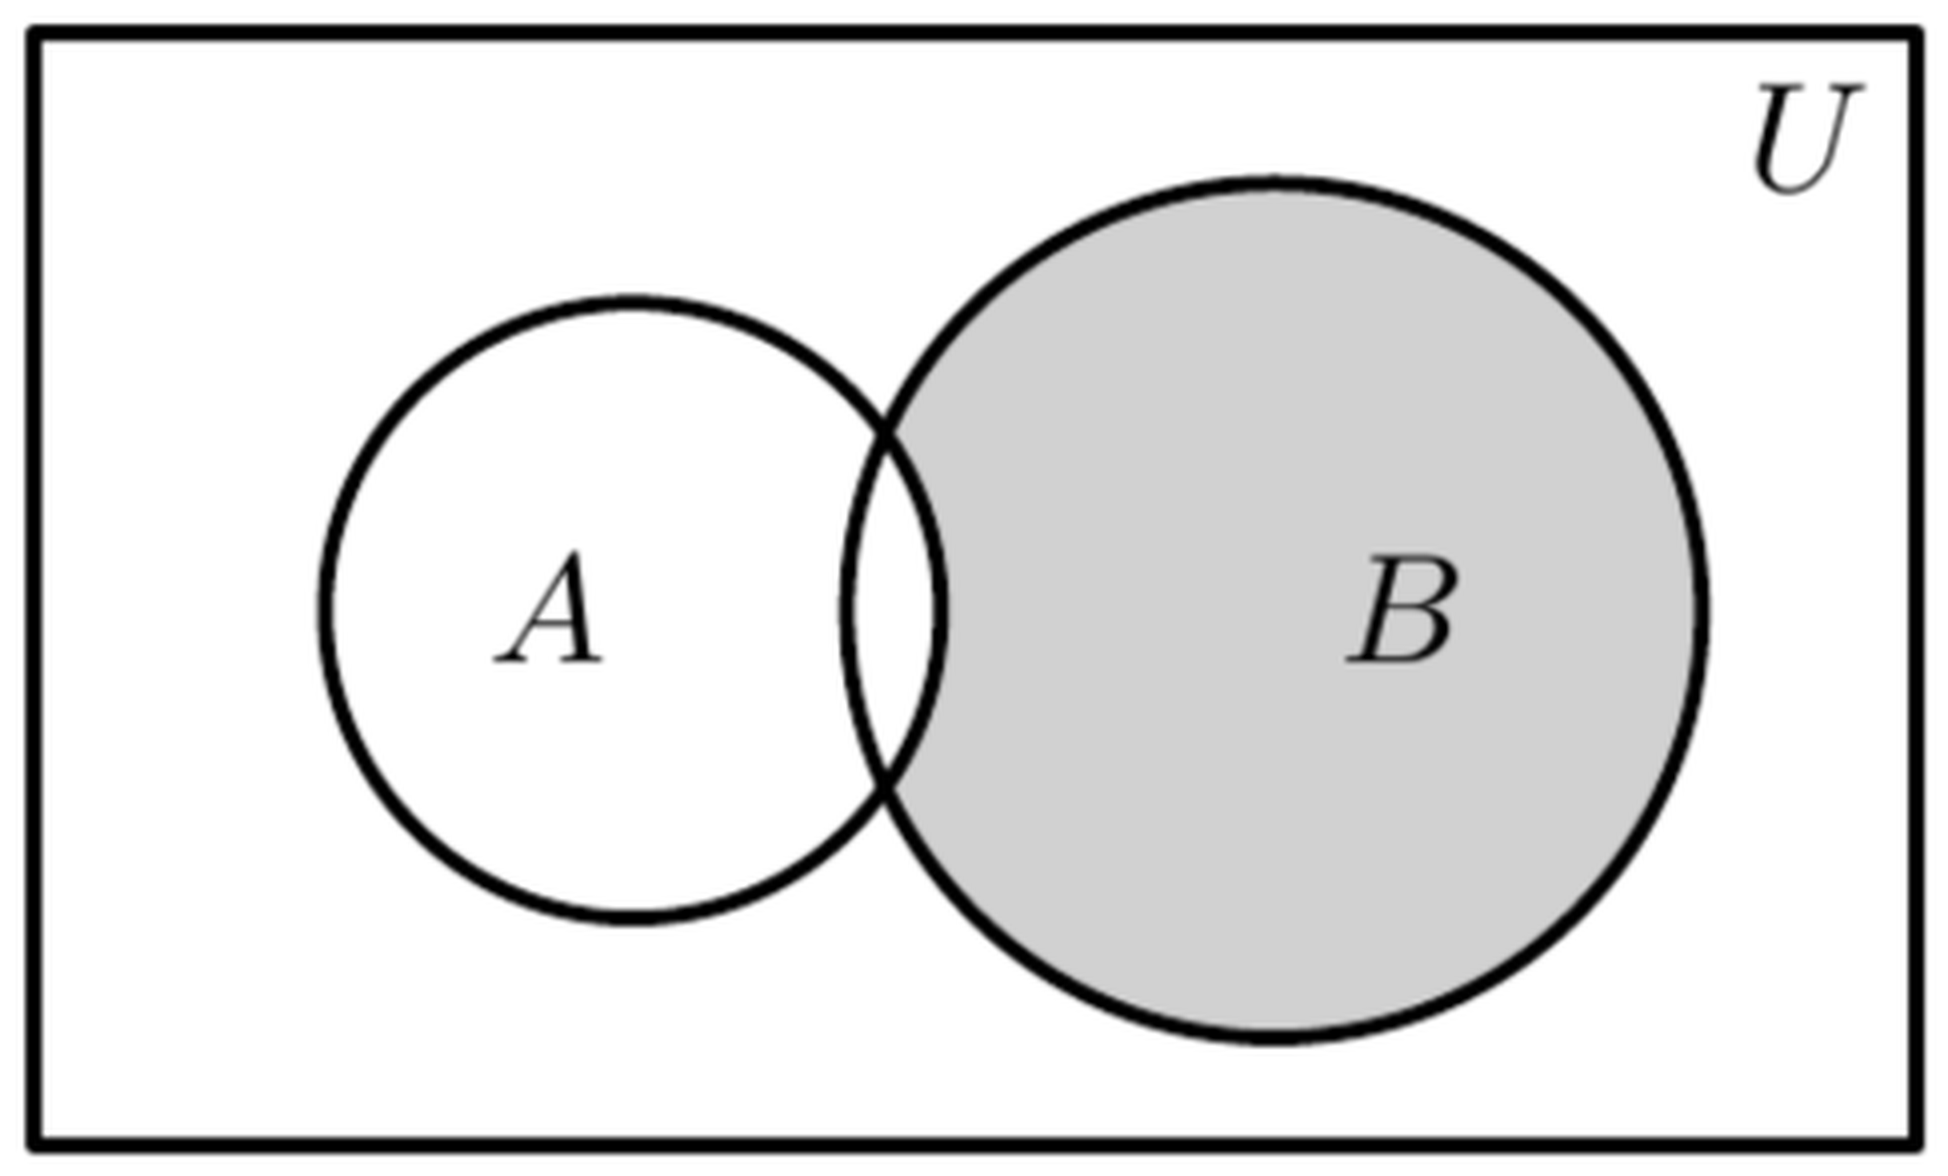
\includegraphics[width=0.38\textwidth]{figures/gao160_q4.png}
\end{center}

\ifanswer
\solbegin
\step{阴影部分表示 $B\cap\overline{A}=\{1,2\}$.}
\solend
\fi

% === Q5 === "图像"（有亻）照录；解析 1 行
\item 已知常数 $a>0$ 且 $a\ne1$，假设无论 $a$ 取何值，函数 $y=\log_a(5x-9)-4$ 的图像恒过一个定点，则这个定点的坐标为\blankline[4.4em].

\ifanswer
\solbegin
\step{$5x-9=1\Rightarrow x=2$，此时 $y=\log_a 1-4=-4$，定点为 $(2,-4)$.}
\solend
\fi

% === Q6 === 解析 2 行
\item 不等式 $(1-2x)^{\frac{3}{4}}>x^{\frac{3}{4}}$ 的解集为\blankline[4.4em].

\ifanswer
\solbegin
\step{定义域为 $\left[0,\dfrac{1}{2}\right]$，由幂函数的单调性，原不等式等价于 $1-2x>x$，}
\step{得 $0\leqslant x<\dfrac{1}{3}$，故解集为 $\left[0,\dfrac{1}{3}\right)$.}
\solend
\fi

% === Q7 === 绝对值 \lvert…\rvert；解析 2 行（跨 01—02 页）
\item 已知不等式 $\lvert x+3\rvert+\lvert x-2\rvert\geqslant 5$，当其等号成立时，$x$ 的取值范围是\blankline[4.4em].

\ifanswer
\solbegin
\step{$\lvert x+3\rvert+\lvert x-2\rvert=\lvert x+3\rvert+\lvert 2-x\rvert\geqslant\lvert(x+3)+(2-x)\rvert=5$，}
\step{等号成立当且仅当 $(x+3)(2-x)\geqslant0$，即 $x\in[-3,2]$.}
\solend
\fi

% === Q8 === 解析 4 行
\item 已知函数 $f(x)=\lvert\log_2 x\rvert$，若方程 $f(x)-t=0$ 有两个不同的实数根 $x_1,x_2$，则 $x_1+x_2$ 的取值范围是\blankline[4.4em].

\ifanswer
\solbegin
\step{方程有两个不同实根，必有 $t>0$，两根为 $2^t,2^{-t}$，}
\step{所以 $x_1+x_2=2^t+2^{-t}>2$（等号仅在 $t=0$ 时成立）.}
\step{任取 $s>2$，令 $a=\dfrac{s+\sqrt{s^2-4}}{2}>1$，取 $t=\log_2 a>0$，则 $x_1+x_2=a+\dfrac{1}{a}=s$，}
\step{所以取值范围为 $(2,+\infty)$.}
\solend
\fi

% === Q9 === 中文弯引号、\R、绝对值 \lvert…\rvert；解析 4 行
\item 已知 $a\in\R$，$b\in\R$，$p:\dfrac{1}{\lvert a\rvert}>\dfrac{1}{\lvert b\rvert}$，$q:\dfrac{1}{a}>\dfrac{1}{b}$，则 $p$ 是 $q$\blankline[4.4em]条件（用“充分非必要”、“必要非充分”、“充要”或“既非充分又非必要”填空）.

\ifanswer
\solbegin
\step{由 $p$、$q$ 中的分式有意义，$a\ne0$ 且 $b\ne0$.}
\step{当 $a=-1,b=-2$ 时，$p$ 成立而 $q$ 不成立，故 $p$ 不是 $q$ 的充分条件.}
\step{当 $a=1,b=-1$ 时，$q$ 成立而 $p$ 不成立，故 $p$ 不是 $q$ 的必要条件.}
\step{故 $p$ 是 $q$ 的充分非必要条件.}
\solend
\fi

% === Q10 === 解析 3 行；其后独立【注】按语 5 行（见头注 ② ⑯、⑤ 1）
\item 已知常数 $a>0$，函数 $y=\dfrac{2^x}{2^x+ax}$ 的图像经过点 $P\left(p,\dfrac{5}{6}\right)$、$Q\left(q,\dfrac{1}{6}\right)$，若 $2^{p+q}=3pq$，则 $a=$\blankline[4.4em].

\ifanswer
\solbegin
\step{由 $\dfrac{2^p}{2^p+ap}=\dfrac{5}{6}$ 得 $2^p=5ap$；由 $\dfrac{2^q}{2^q+aq}=\dfrac{1}{6}$ 得 $2^q=\dfrac{aq}{5}$.}
\step{$2^p>0$，$2^q>0$，$a>0$，得 $p>0$，$q>0$.}
\step{两式相乘得 $2^{p+q}=a^2pq$，又 $2^{p+q}=3pq$ 且 $pq\ne0$，故 $a^2=3$，$a=\sqrt{3}$.}
\solend
% 【注】按语（讲评版编者按，5 个印刷行，仅答案版出，不属于任何题的【解析】）
\stepm{【注】}{按原卷数据严格推敲，点 $Q$ 其实不存在：$a=\sqrt{3}$ 时 $2^q=\dfrac{\sqrt{3}}{5}q<q$；而当 $q>0$}
\step{时，取非负整数 $n$ 使 $n\leqslant q<n+1$，由 $2^{k+1}=2^k+2^k\geqslant2^k+1$ 逐次推得 $2^n\geqslant n+1$，于是}
\step{$2^q\geqslant2^n\geqslant n+1>q$，矛盾. 所以题设条件互相矛盾，严格说本题无解；$\sqrt{3}$ 是由题给关}
\step{系直接推出的值，按命题意图作为答案. 原卷数据疑似有误（同型常见题为 $P\left(p,\dfrac{6}{5}\right)$、}
\step{$Q\left(q,-\dfrac{1}{5}\right)$、$2^{p+q}=36pq$，得 $a=6$）.}% 见头注 ⑤ 1，照录未改
\fi

% === Q11 === 纳皮尔对数材料题；\Z、大数；解析 6 行
\item 17 世纪初，约翰·纳皮尔为了简化计算而发明了对数. 对数的发明是数学史上的重大事件，恩格斯曾经把笛卡尔的坐标系、纳皮尔的对数、牛顿和莱布尼兹的微积分共同称为 17 世纪的三大数学发明. 我们知道，任何一个正实数 $N$ 可以表示成 $N=a\times10^n$ ($1\leqslant a<10,n\in\Z$) 的形式，这便是科学记数法，若两边取常用对数，有 $\lg N=n+\lg a$，则可以估计 $3^{2026}$ 的最高位上的数值为\blankline[4.4em].

\ifanswer
\solbegin
\step{设 $3^{2026}=a\times10^n$ ($1\leqslant a<10,n\in\Z$)，则 $2026\lg 3=n+\lg a$.}
\step{用 $\lg 3\approx 0.4771$ 粗估，得 $2026\lg 3\approx 966.60$.}
\step{为核验误差，用 $0.47712<\lg 3<0.47713$，}
\step{得 $966.64512<2026\lg 3<966.66538$，因此 $n=966$.}
\step{于是 $\lg 4\approx 0.60206<0.64512<\lg a<0.66538<\lg 5\approx 0.69897$，}
\step{所以 $4<a<5$，最高位为 4，估算误差不影响结论.}
\solend
\fi

% === Q12 === 自定义"性质 P"；文本圈数字①②③；解析 19 行（跨 03—05 页）
\item 对于数集 $X=\{-1,x_1,x_2,x_3,\cdots,x_n\}$，其中 $0<x_1<x_2<x_3<\cdots<x_n$，$n\geqslant2$，定义点集 $Y=\{(s,t)\mid s\in X,t\in X\}$，若对于任意 $(s_1,t_1)\in Y$，存在 $(s_2,t_2)\in Y$，使得 $s_1s_2+t_1t_2=0$，则称集合 $X$ 具有性质 $P$. 则下列命题中为真命题的是\blankline[4.4em].

① $X=\{-1,1,2\}$ 具有性质 $P$；②若集合 $X$ 具有性质 $P$，则 $1\in X$；

③集合 $X$ 具有性质 $P$，若 $x_1=\dfrac{1}{2}$，则 $x_n=2$.

\ifanswer
\solbegin
\step{因为 $X=\{-1,1,2\}$，}
\step{所以 $Y=\{(-1,-1),(1,1),(2,2),(-1,1),(-1,2),(1,-1),(1,2),(2,-1),(2,1)\}$，}
\step{由集合 $X$ 具有性质 $P$ 的定义，对于任意 $(s,t)\in Y$，}
\step{若 $s>0$，$t>0$，则 $s=t$ 或 $(s,t)=(1,2)$ 或 $(s,t)=(2,1)$，}
\step{若 $s=t$，取 $s_2=-1$，$t_2=-1$，则 $ss_2+tt_2=0$；}
\step{若 $(s,t)=(1,2)$，取 $s_2=2$，$t_2=-1$，则 $ss_2+tt_2=0$；}
\step{若 $(s,t)=(2,1)$，取 $s_2=-1$，$t_2=2$，则 $ss_2+tt_2=0$；}
\step{若 $s$、$t$ 有一个为负数，则 $s=-1$ 或 $t=-1$，}
\step{若 $s=-1$，则取 $s_2=t$，$t_2=1$，则 $ss_2+tt_2=0$；}
\step{若 $t=-1$，则取 $s_2=1$，$t_2=s$，则 $ss_2+tt_2=0$；故①正确；}
\step{对于任意 $(s_1,t_1)\in Y$，存在 $(s_2,t_2)\in Y$，使得 $s_1s_2+t_1t_2=0$，}
\step{取 $(x_1,x_1)\in Y$，存在 $(x_p,x_q)$ 使得 $x_1x_p+x_1x_q=0$，所以 $x_p+x_q=0$，}
\step{不妨设 $x_p=1$，$x_q=-1$，所以若集合 $X$ 具有性质 $P$，则 $1\in X$，故②正确；}
\step{③假设 $x_n>1$，令 $s_1=\dfrac{1}{2},t_1=x_n$，则存在 $s$、$t\in X$ 使得 $\dfrac{1}{2}s+tx_n=0$，}
\step{同②得 $s$、$t$ 中必有一个数为 $-1$，}
\step{若 $s=-1$，则 $tx_n=\dfrac{1}{2}$，于是 $t=\dfrac{1}{2x_n}<\dfrac{1}{2}=x_1$，矛盾，}
\step{若 $t=-1$，则 $\dfrac{1}{2}s=x_n\cdot(-1)$，于是 $s=2x_n>x_n$，也矛盾，}% 原卷如此（与结论符号不自洽），照录未改，见头注 ⑤ 2
\step{所以 $x_n\leqslant1$，又由②得 $1\in X$，所以 $x_n\geqslant1$，所以 $x_n=1$，故③错误，}
\step{故真命题是①②.}
\solend
\fi

\end{enumerate}

% 答案版里填空解析把页排满，节标题会落到页末、与第 13 题分家（切页审计 B 类）；
% 守卫放 \bigsec 之前，连节标题一起量页高（高一157 成例）
\needvspace{7cm}
\bigsec{二、选择题}

\begin{enumerate}
\setcounter{enumi}{12}

% === Q13 === "图像"照录；解析 1 行，故选 $B$
\item 下列函数中，图像与函数 $y=3^x$ 图像关于 $y$ 轴对称的是\mbox{（\quad）}

\keepwithprev
A. $y=x^3$\qquad B. $y=\left(\dfrac{1}{3}\right)^x$\qquad C. $y=-3^x$\qquad D. $y=\log_3 x$

\ifanswer
\solbegin
\step{将 $x$ 换为 $-x$，得对称图像对应的函数为 $y=3^{-x}=\left(\dfrac{1}{3}\right)^x$，故选 $B$.}
\solend
\fi

% === Q14 === 中文弯引号；解析 2 行（跨 05 页上下），故选 $B$
\item 命题“存在 $x\in(1,+\infty)$，使得 $f(x)>0$”的否定形式为\mbox{（\quad）}

\keepwithprev
A. 不存在 $x\in(-\infty,1]$，使得 $f(x)>0$\qquad B. 对任意 $x\in(1,+\infty)$，有 $f(x)\leqslant0$

C. 对任意 $x\in(-\infty,1]$，有 $f(x)\leqslant0$\qquad D. 存在 $x\in(1,+\infty)$，使得 $f(x)\leqslant0$

\ifanswer
\solbegin
\step{将“存在”改为“对任意”，$x$ 的范围不变，并将 $f(x)>0$ 否定为 $f(x)\leqslant0$，}
\step{故选 $B$.}
\solend
\fi

% === Q15 === \R；四选项两行；解析 3 行，故选 $D$
\item 设 $a>0$，$s\in\R$. 下列各项中，能推出 $a^s>a$ 的一项是\mbox{（\quad）}

\keepwithprev
A. $a>1$，且 $s>0$\qquad B. $a>1$，且 $s<0$

C. $0<a<1$，且 $s>0$\qquad D. $0<a<1$，且 $s<0$

\ifanswer
\solbegin
\step{当 $a>1$ 时，$a^s>a\Leftrightarrow s>1$，A、B 均不能保证.}
\step{当 $0<a<1$ 时，$a^s>a\Leftrightarrow s<1$，C 不能保证，D 中 $s<0<1$，满足要求；}
\step{故选 $D$.}
\solend
\fi

% === Q16 === 题目配图（三版都出）；几何符号 \triangle ABC；解析 3 行，故选 $C$
\needvspace{8cm}
\item 数学说明的方法多种多样，其中利用图形说明就是一种重要方法. 如图所示，在等腰直角三角形 $\triangle ABC$ 中，点 $O$ 为斜边 $AB$ 的中点，点 $D$ 为斜边 $AB$ 上异于顶点的一个动点，设 $AD=a$，$BD=b$，则可用该图形能说明的不等式为\mbox{（\quad）}

\begin{center}
% Q16 等腰直角三角形 ABC 图（C/A/O/D/B 标注）取 05 页右下，去粉色水印、去色、3× LANCZOS 放大；三版都出
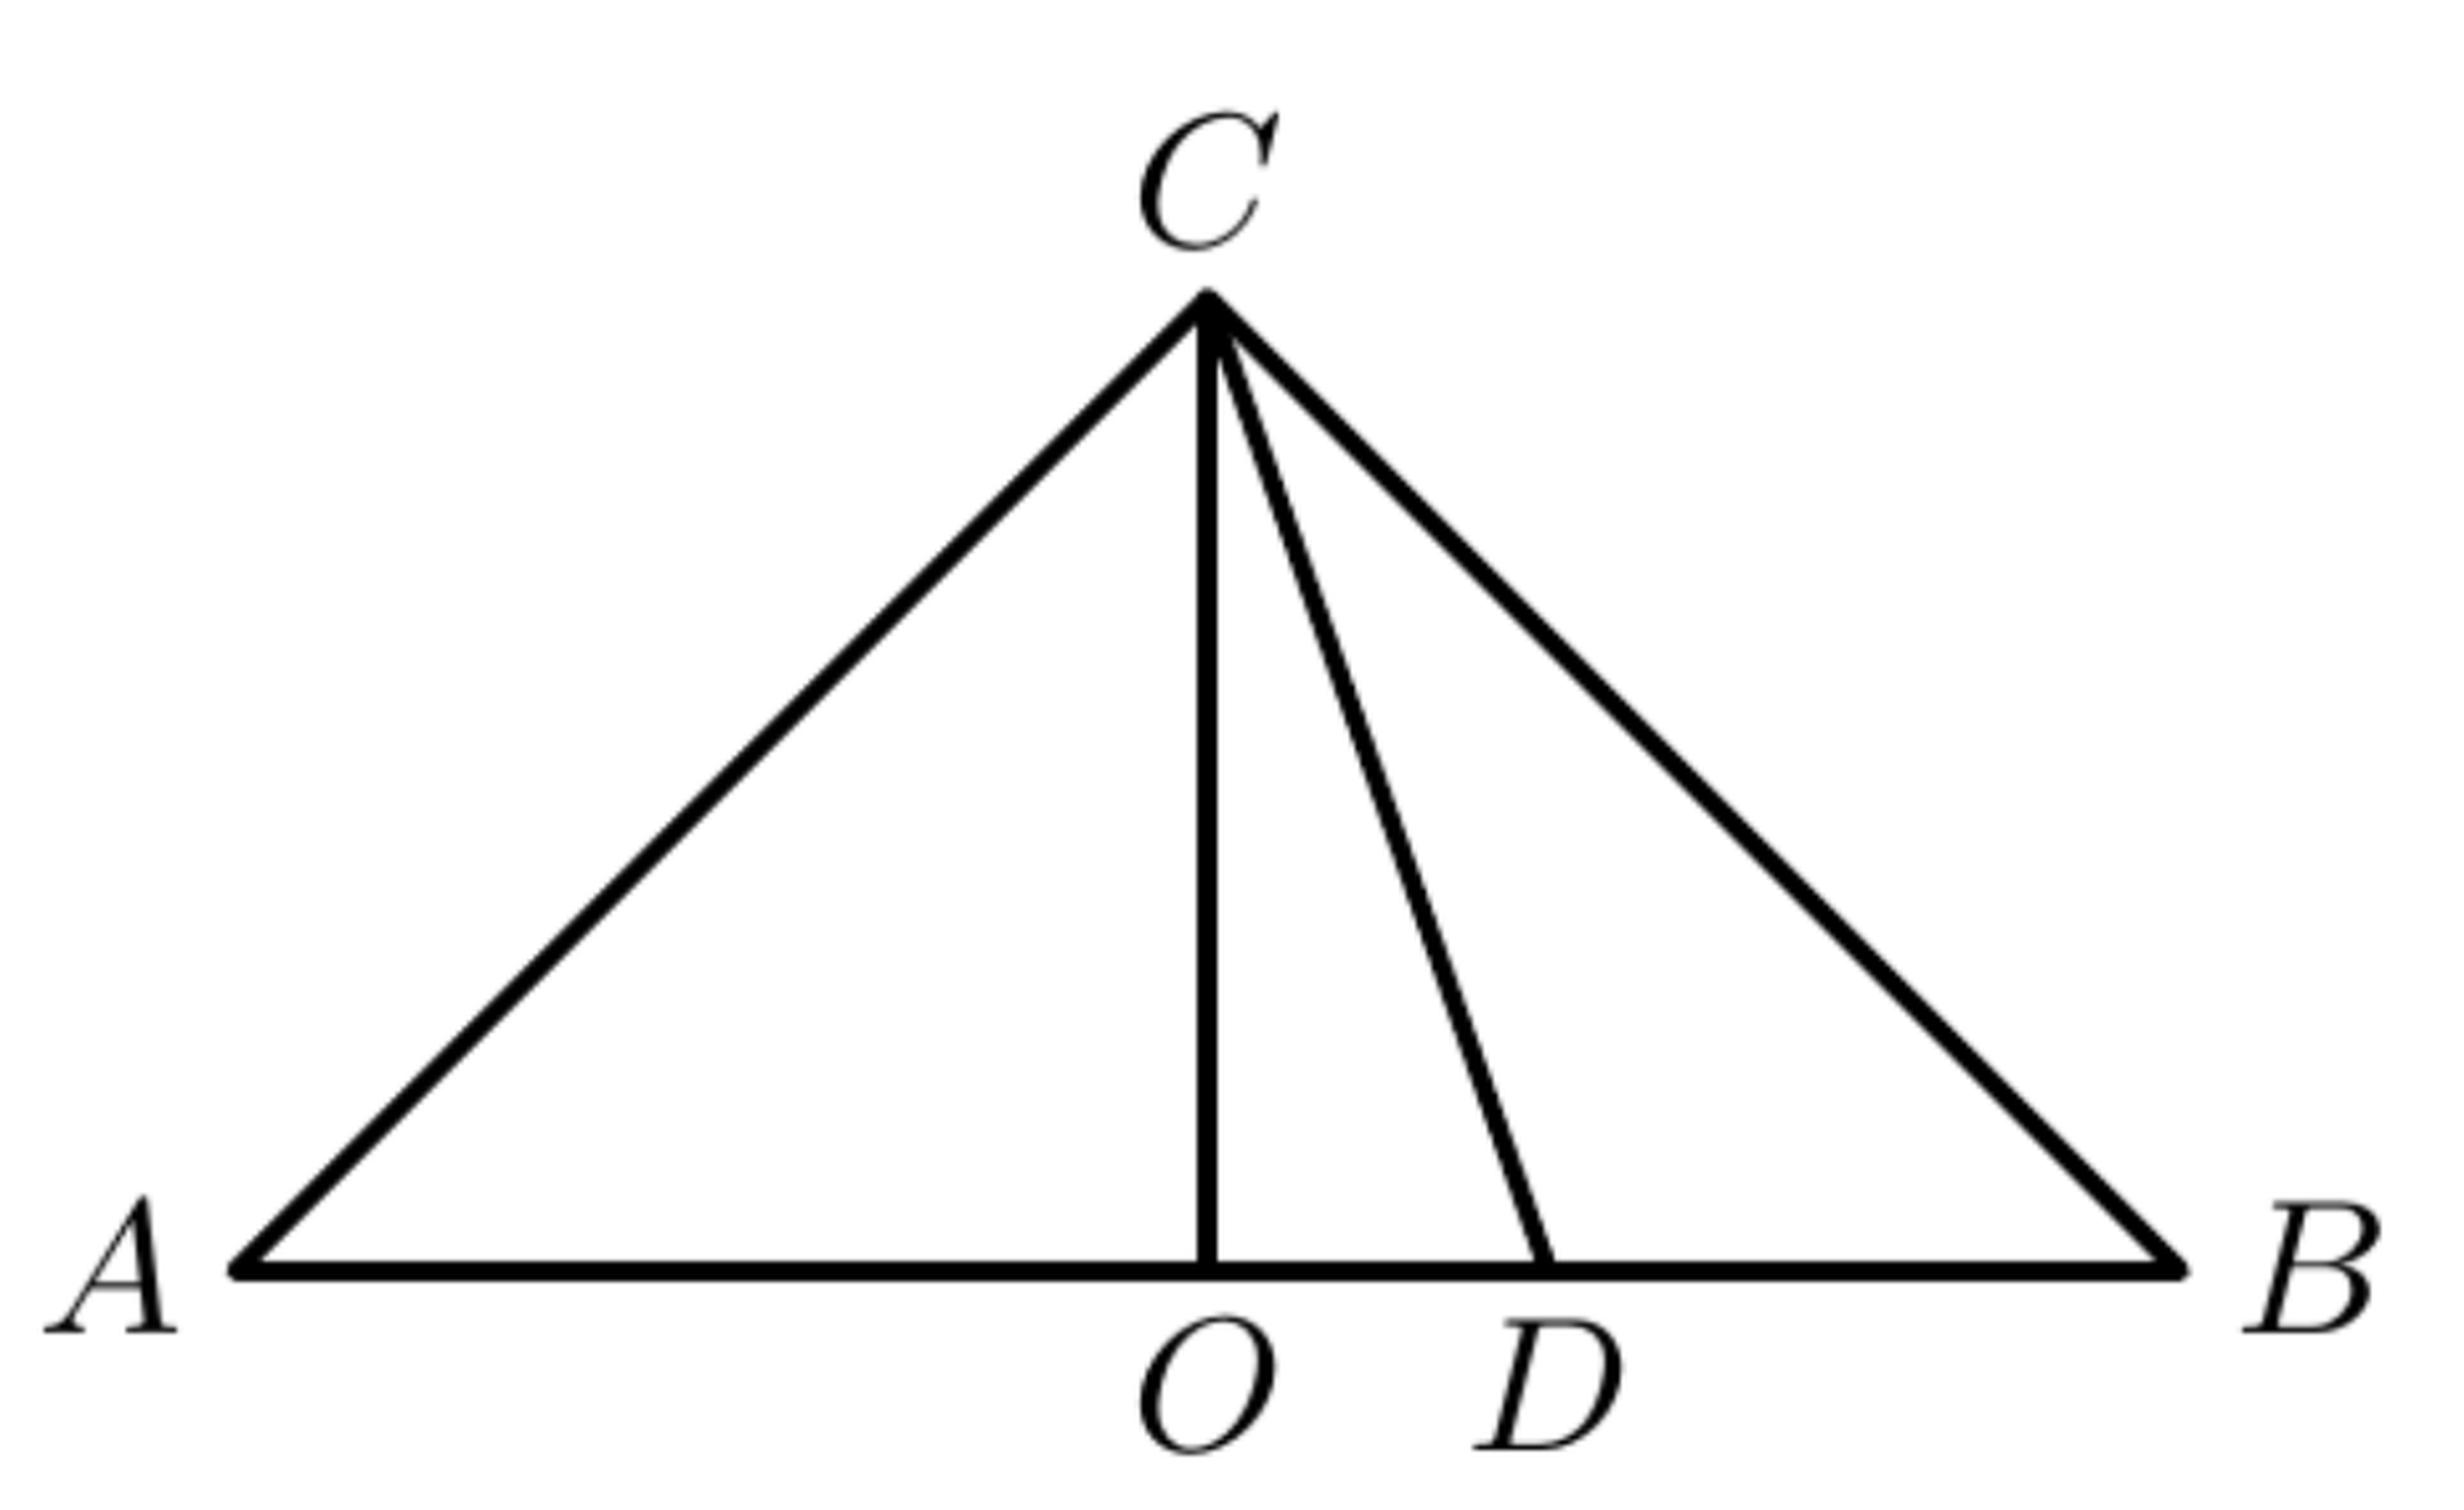
\includegraphics[width=0.34\textwidth]{figures/gao160_q16.png}
\end{center}

\keepwithprev
A. $\dfrac{a+b}{2}\geqslant\sqrt{ab}$ ($a>0,b>0$)\qquad B. $a^2+b^2\geqslant2\sqrt{ab}$ ($a>0,b>0$)

C. $\dfrac{a+b}{2}\leqslant\sqrt{\dfrac{a^2+b^2}{2}}$ ($a>0,b>0$)\qquad D. $\dfrac{2ab}{a+b}\leqslant\sqrt{ab}$ ($a>0,b>0$)

\ifanswer
\solbegin
\step{$CO=AO=\dfrac{a+b}{2},OD=\left\lvert a-\dfrac{a+b}{2}\right\rvert=\dfrac{\lvert a-b\rvert}{2}$，}
\step{$CD=\sqrt{CO^2+OD^2}=\sqrt{\dfrac{a^2+b^2}{2}}\geqslant CO=\dfrac{a+b}{2}$，}
\step{等号当且仅当 $a=b$ 时成立，故选 $C$.}
\solend
\fi

\end{enumerate}

\bigsec{三、解答题}

\begin{enumerate}
\setcounter{enumi}{16}

% === Q17 === cases 块算一行；判别式印等腰偏高三角 \Delta；解析 7 行
\item 已知幂函数 $f(x)=(m^2-2m-2)x^{m-1}$ 在 $(0,+\infty)$ 上是严格增函数.

(1) 求 $m$ 的值；

(2) 若关于 $x$ 的方程 $f(x)=(t+1)x-t^2$ 有两个不相等的正实根，求实数 $t$ 的取值范围.

\ifanswer
\solbegin
\step{(1) 幂函数的系数为 1，因此 $m^2-2m-2=1\Leftrightarrow(m-3)(m+1)=0$，}
\step{解得 $m=3$ 或 $m=-1$.}
\step{由 $f(x)$ 在 $(0,+\infty)$ 上严格递增，得 $m-1>0$，所以 $m=3$，}
\step{此时 $f(x)=x^2$.}
\step{(2) 原方程化为 $x^2-(t+1)x+t^2=0$，}
\step{方程有两个不相等的正实根，则 $\begin{cases}\Delta=(t+1)^2-4t^2=(1-t)(3t+1)>0\\t+1>0\\t^2>0\end{cases}$，}% 判别式原卷印等腰偏高三角 \Delta，照录
\step{得 $t\in\left(-\dfrac{1}{3},0\right)\cup(0,1)$.}
\solend
\fi

% === Q18 === 补集上划线 \overline{A}、\subseteq 带下划线、\varnothing；解析 8 行
\item 已知集合 $A=\{x\mid\lvert x-a\rvert<a-3\}$，$B=\left\{x\mid\dfrac{x+1}{x-2}\geqslant2\right\}$.

(1) 若 $a=5$，求 $\overline{A}\cap B$；

(2) 若 $A\cap B=A$，求实数 $a$ 的取值范围.

\ifanswer
\solbegin
\step{(1) $\dfrac{x+1}{x-2}\geqslant2\Leftrightarrow\dfrac{5-x}{x-2}\geqslant0\Leftrightarrow2<x\leqslant5,B=(2,5]$，}
\step{当 $a=5$ 时，$A=\{x\mid\lvert x-5\rvert<2\}=(3,7)$，于是 $\overline{A}=(-\infty,3]\cup[7,+\infty)$，}
\step{因此 $\overline{A}\cap B=(2,3]$.}
\step{(2) $A\cap B=A$ 等价于 $A\subseteq B$.}
\step{当 $a\leqslant3$ 时，$a-3\leqslant0$，$A=\varnothing$，满足条件.}
\step{当 $a>3$ 时，$\lvert x-a\rvert<a-3\Leftrightarrow3<x<2a-3,A=(3,2a-3)$，}
\step{此时 $A\subseteq B=(2,5]$ 等价于 $2a-3\leqslant5$，即 $a\leqslant4$，结合 $a>3$ 得 $3<a\leqslant4$.}
\step{合并两种情形，实数 $a$ 的取值范围为 $(-\infty,4]$.}
\solend
\fi

% === Q19 === 数据表 tabular 重排（高一130 成例）；cases 块算一行；解析 6 行
\item 作为我国最高水平的综合性运动会，全运会汇聚了国内顶尖体育健儿，某代表队从第 8 届全运会开始登上赛场，且参赛运动员人数逐年递增. 设 $t$ 为该代表队参赛后经过的届数，即第 8 届为 $t=0$，第 9 届为 $t=1$，以此类推. 经过 $t$ 届，运动员人数为 $y$ 人，具体数据如下：

\begin{center}
\begin{tabular}{cccccc}
$t$ & 0 & 1 & 2 & 3 & 4 \\
\hline
届数 & 8 & 9 & 10 & 11 & 12 \\
运动员人数（$y$ 人） & 4 & 11 & 25 & 53 & 109
\end{tabular}
\end{center}

(1) 现有以下两种函数模型：① $y=a\cdot b^t+c$ ($a>0,b>1$)；② $y=\log_a(t+b)+c$ ($b>0,a>1$). 请根据上表中运动员人数的增长规律，选出你认为符合的函数模型（不用说明理由），并利用表中前 3 组数据求出相应的函数解析式；

(2) 若参赛运动员人数按照 (1) 中求得的模型继续增长，在第几届全运会时，该代表队运动员人数将会首次超过 1000 人？

\ifanswer
\solbegin
\step{(1) 选模型①，将前 3 组数据代入，得 $\begin{cases}a+c=4\\ab+c=11\\ab^2+c=25\end{cases}$，}% 原卷印"选模型①"（圈数字①），OCR 误作"四"，照录①，见头注 ⑤ 3
\step{相邻两式相减，得 $a(b-1)=7$，$ab(b-1)=14$，}
\step{两式相除得 $b=2$，进而 $a=7$，$c=-3$，所求函数解析式为 $y=7\cdot2^t-3$.}
\step{(2) $y=7\cdot2^t-3$ 随 $t$ 的增大而增大，且 $t=7$ 时，$y=893<1000$；}
\step{$t=8$ 时，$y=1789>1000$，}
\step{$t$ 为非负整数，首次超过 1000 人时 $t=8$，对应第 $8+8=16$ 届全运会.}
\solend
\fi

% === Q20 === 解析 12 行（跨 08—09 页）
\item 已知函数 $f(x)=\log_a(a-a^x)$.

(1) 求该函数的定义域；

(2) 若 $a>1$，试判断关于 $x$ 的方程 $f(x)=2$ 是否有实数解，并说明理由；

(3) 若当 $x\in(-\infty,0]$ 时，关于 $x$ 的不等式 $f(x)\geqslant-1$ 恒成立，求实数 $a$ 的取值范围.

\ifanswer
\solbegin
\step{(1) 对数的底数须满足 $a>0$ 且 $a\ne1$，真数须满足 $a-a^x>0$，即 $a^x<a^1$.}% 原卷印 $a^1$，照录未化简，见头注 ⑤ 4
\step{当 $a>1$ 时，$x<1$，定义域为 $(-\infty,1)$.}
\step{当 $0<a<1$ 时，$x>1$，定义域为 $(1,+\infty)$.}
\step{(2) 当 $a>1$ 时，若 $f(x)=2$，则 $a-a^x=a^2\Rightarrow a^x=a(1-a)<0$，}
\step{这与 $a^x>0$ 矛盾，因此方程无实数解.}
\step{(3) 不等式在 $(-\infty,0]$ 上恒成立，须先保证该区间包含于函数的定义域，}
\step{由 (1) 得 $a>1$.}
\step{当 $x\leqslant0$ 时，$0<a^x\leqslant1$，所以 $a-a^x\geqslant a-1>0$.}
\step{由对数函数的单调性，$f(x)=\log_a(a-a^x)\geqslant\log_a(a-1)=f(0)$，}
\step{等号当且仅当 $x=0$ 时成立，}
\step{因此所求条件等价于 $\log_a(a-1)\geqslant-1\Leftrightarrow a-1\geqslant\dfrac{1}{a}\Leftrightarrow a^2-a-1\geqslant0$，}
\step{结合 $a>1$，得 $a\in\left[\dfrac{1+\sqrt{5}}{2},+\infty\right)$.}
\solend
\fi

% === Q21 === "和积平衡集"定义证明题；\N；解析 18 行（跨 09—10 页）
\item 已知有限集 $A=\{a_1,a_2,\cdots,a_n\}$ ($n\geqslant2,n\in\N$)，如果 $A$ 中元素 $a_i$ ($i=1,2,3,\cdots,n$) 满足 $a_1+a_2+a_3+\cdots+a_n=a_1\times a_2\times\cdots\times a_n$，就称 $A$ 为“和积平衡集”.

(1) 分别判断集合 $A=\{1,2,3,4\}$，$B=\{4+2\sqrt{2},4-2\sqrt{2}\}$ 是否为“和积平衡集”；

(2) 已知 $a_1$、$a_2$ 是两个不同的正数，且 $\{a_1,a_2\}$ 是“和积平衡集”，请用反证法证明：$a_1$、$a_2$ 至少有一个大于 2；

(3) 若 $a_i\geqslant1$，且 $a_i\in\N$，求所有符合条件的“和积平衡集”.

\ifanswer
\solbegin
\step{(1) 因为 $1+2+3+4=10\ne24=1\times2\times3\times4$，所以 $A$ 不是“和积平衡集”.}
\step{因为 $(4+2\sqrt{2})+(4-2\sqrt{2})=8=(4+2\sqrt{2})(4-2\sqrt{2})$，}
\step{所以 $B$ 是“和积平衡集”.}
\step{(2) 假设 $a_1$、$a_2$ 都不大于 2，则 $\dfrac{1}{a_1}\geqslant\dfrac{1}{2},\dfrac{1}{a_2}\geqslant\dfrac{1}{2}$，}
\step{由于 $a_1\ne a_2$，上述两个不等式至少有一个严格成立.}
\step{而 $a_1+a_2=a_1a_2$，两边除以 $a_1a_2>0$，得 $1=\dfrac{1}{a_1}+\dfrac{1}{a_2}>\dfrac{1}{2}+\dfrac{1}{2}=1$，矛盾，}
\step{所以 $a_1$、$a_2$ 至少有一个大于 2.}
\step{(3) 不妨设 $a_1<a_2<\cdots<a_n$，由各元素均为正整数，得 $a_i\geqslant i$.}
\step{若 $n\geqslant4$，因其余因子均不小于 1，}
\step{有 $a_1a_2\cdots a_n\geqslant a_2a_{n-1}a_n\geqslant2(n-1)a_n>na_n>a_1+a_2+\cdots+a_n$，}
\step{与和积平衡条件矛盾，因此只需讨论 $n=2,3$.}
\step{当 $n=2$ 时，$a_1+a_2=a_1a_2\Leftrightarrow(a_1-1)(a_2-1)=1$，}
\step{两个因子均为非负整数，只能有 $a_1=a_2=2$，与元素互不相同矛盾.}
\step{当 $n=3$ 时，若 $a_1\geqslant2$，则 $a_2\geqslant3$，从而 $a_1a_2a_3\geqslant6a_3>3a_3>a_1+a_2+a_3$，}
\step{矛盾，因此 $a_1=1$.}
\step{此时 $1+a_2+a_3=a_2a_3\Leftrightarrow(a_2-1)(a_3-1)=2$，}
\step{由 $1\leqslant a_2-1<a_3-1$，得 $a_2-1=1$、$a_3-1=2$，即 $a_2=2$、$a_3=3$.}
\step{检验 $1+2+3=1\times2\times3=6$，所求集合为 $\{1,2,3\}$.}
\solend
\fi

\end{enumerate}

\end{document}
"
%
% ① 原始材料：微信公众号"魔都数学加油站"文章，连载"27学年高一160"，原卷卷面标题
% "2026-2027 年奉贤中学高一上期中"（卷面未印副标题、未印连载号）。
% 正文为 10 张 PNG 页（01/04/10 为 2560×3620，02/03/05/06/07/08/09 为
% 4762×6735，同一篇各页分辨率混排，逐页按各自分辨率裁图核对）。
% 体例：讲评版——填空 3—12（10 题）、选择 13—16（4 题）、解答 17—21（5 题），
% 共 19 题，自第 3 题起编（1、2 未印在本篇）；19 题逐题印【解析】，无只印【答案】
% 的题；四道选择题答案在解析末句"故选 $B$/$B$/$D$/$C$"，题干括号
% \mbox{（\quad）} 留空、不另提 \ans{}。题目、答案、解析均据原图转录；卷面粉红色
% 水印"魔都数学加油站"及公众号页脚未录入。
% 全卷插图清单（逐页通读 10 页确认）：2 幅，均为题目配图、三版都出——
%   · Q4 韦恩图（01 页右侧：矩形全集 U、两圆 A/B、阴影部分 B∩上划线 A、
%     标注 U/A/B），裁 figures/gao160_q4.png；
%   · Q16 等腰直角三角形 ABC 图（05 页右下：C 顶点、A/O/D/B 共线底边、
%     CO 与 CD 两条线段），裁 figures/gao160_q16.png；
%   两图均取原卷截图 3—4× LANCZOS 放大、去粉色水印、转灰度、autocontrast；
%   Q4 图左侧题干残字"示"、Q16 图左侧题干残字均已裁白。
%   Q19 有一张 3 行数据表（t／届数／运动员人数（y 人），t=0..4），按全稿
%   成例（高一130）用 tabular 重排，不做成 png；其余各页无题目配图、
%   无解析内配图、无其它表格、无"如图"处。
%
% 卷首标题：原卷印作"2026-2027 年奉贤中学高一上期中"，年份区间按全稿惯例排 en dash；
% 原卷卷面未印副标题，本稿按同期中卷知识模块口径补出"集合与常用逻辑用语、不等式、函数"。
%
% ② 与原卷的排版差异／照录项清单：
%   ① 原文从第 3 题起，本稿保留原题号；共 19 题三节，解答题 5 题到 21；
%      三节各自一个 enumerate + \setcounter{enumi}{2}/{12}/{16}（不贯穿），
%      用 \examtitlest[3] 起手；
%   ② 混合体例说明：19 题全印【解析】、用 \solbegin…\solend，无只印【答案】
%      或答案印括号内的题；四道选择题答案在解析末句"故选 $B$/$B$/$D$/$C$"
%      （逐个放大复核）、括号 \mbox{（\quad）} 留空、不另提 \ans{}；答案版
%      【答案】/【解析】标记数 = 19 = 全卷题数（0 个 \ans ＋ 19 个 \solbegin）；
%   ③ 原卷卷面未印副标题，本稿按知识模块口径补出；
%   ④ 原卷填空横线按全稿惯例排 \blankline[4.4em]；选择题括号排 \mbox{（\quad）}、
%      四道选择题的选项段前按惯例各加 \keepwithprev；解答题不留作答区、不加
%      \anspace（原卷为讲评版，109—113 起全稿不用 \anspace）；
%   ⑤ 数集归一：Q4"$U=\Z$"、Q9"$a\in\R$，$b\in\R$"、Q11"$n\in\Z$"、
%      Q15"$s\in\R$"、Q21"$n\in\N$""$a_i\in\N$"原卷印正体粗体 Z/R/N，
%      按全稿惯例归一 \Z／\R／\N；集合描述竖线排 \mid（Q3、Q4、Q12、
%      Q18、Q21）；空集 \varnothing（Q18 解析 (2)）；补集照原卷上划线排
%      \overline{A}（Q4 解析、Q18 (1) 题干与解析）；子集符号 Q18 两处
%      "$A\subseteq B$"印带下划线 ⊆、照录 \subseteq；
%   ⑥ 绝对值排 \lvert…\rvert（Q7、Q8 题干与解析、Q9 题干、Q16 解析、
%      Q18 题干与解析），Q16 解析的 \left\lvert…\right\rvert 与 \lvert…\rvert
%      均在同一 $…$ 组内配对平衡；
%   ⑦ 判别式两形混用逐处照录不统一（放大逐处确认）：Q3 解析
%      "$\triangle=1^2-4a\times\frac{1}{4}=0$"原卷印扁等边三角、照录
%      \triangle；Q17 解析 cases 块"$\Delta=(t+1)^2-4t^2=(1-t)(3t+1)>0$"
%      原卷印等腰偏高三角、照录 \Delta；Q16 题干几何符号"$\triangle ABC$"
%      按全稿几何三角形记号惯例归一 \triangle（参照 高一150／132 成例）；
%   ⑧ 不等号按全稿惯例排 \leqslant／\geqslant；中文弯引号照录：Q9 题干
%      "充分非必要""必要非充分""充要""既非充分又非必要"、Q14 题干
%      "存在 $x\in(1,+\infty)$，使得 $f(x)>0$"与解析"存在""对任意"、
%      Q21 题干与解析多处"和积平衡集"；注释里一律 ASCII 引号；
%   ⑨ 文本圈数字逐处照录：Q12 题干①②③、Q12 解析"故①正确""同②得"
%      "故②正确""③假设""故③错误""故真命题是①②"、Q19 题干①②与解析
%      "选模型①"，均为印刷圈数字（非 \textcircled、非数学模式）；
%   ⑩ 半角逗号在数学组之间是全稿惯例、非笔误，逐处照录（Q8"$2^t,2^{-t}$"、
%      Q9"$a=-1,b=-2$""$a=1,b=-1$"、Q11"$1\leqslant a<10,n\in\Z$"、
%      Q12"$s_1=\frac{1}{2},t_1=x_n$"、Q16 选项"$a>0,b>0$"与解析
%      "$CO=AO=\frac{a+b}{2},OD=...$"、Q18"$2<x\leqslant5,B=(2,5]$"
%      "$3<x<2a-3,A=(3,2a-3)$"、Q21"$n=2,3$"等）；行中全角逗号／顿号
%      照录（Q15 选项"$a>1$，且 $s>0$"、Q12 解析"$s$、$t$"、Q21 解析
%      "$a_1$、$a_2$"），顿号一律移出数学模式；
%   ⑪ "图像／图象"逐处照录：本卷 Q5"的图像恒过一个定点"、Q10"的图像经过点"、
%      Q13 题干两处"图像"与解析"对称图像对应的函数"均印"图像"（有亻）；
%      Q16 印"图形"（利用图形说明、该图形能说明），无"图象"用例；
%   ⑫ 复杂式照录别简化：Q3 $ax^2+x+\frac14=0$、Q5 $y=\log_a(5x-9)-4$、
%      Q6 $(1-2x)^{\frac34}>x^{\frac34}$ 与 $\left[0,\frac12\right]$、
%      Q8 $\frac{s+\sqrt{s^2-4}}{2}$、Q10 $y=\frac{2^x}{2^x+ax}$ 与
%      $\frac{2^p}{2^p+ap}=\frac56$、$\frac{2^q}{2^q+aq}=\frac16$、
%      Q11 $N=a\times10^n$ 与 $3^{2026}$、$2026\lg3\approx966.60$、
%      $966.64512<2026\lg3<966.66538$、Q12 $Y=\{(s,t)\mid s\in X,t\in X\}$
%      与 $\frac12 s+tx_n=0$、Q16 $\sqrt{\frac{a^2+b^2}{2}}$、
%      Q17 $x^2-(t+1)x+t^2=0$ 与 $\left(-\frac13,0\right)\cup(0,1)$、
%      Q18 $\frac{5-x}{x-2}\geqslant0$、Q19 $y=a\cdot b^t+c$ 与
%      $y=\log_a(t+b)+c$、$y=7\cdot2^t-3$、Q20 $f(x)=\log_a(a-a^x)$
%      与 $a^2-a-1\geqslant0$、$\left[\frac{1+\sqrt5}{2},+\infty\right)$、
%      Q21 $4+2\sqrt2$ 与 $(a_2-1)(a_3-1)=2$ 等；
%   ⑬ 子题标号 (1)(2)(3) 按全稿惯例排半角括号；行末／行中句点按全稿惯例
%      排 ASCII `.`（不是全角「．」）；cases 块整体算一个印刷行
%      （Q17 解析、Q19 解析 (1)）；
%   ⑭ 配图：Q4／Q16 题目配图（三版都出）放 \item 内题干之后 \begin{center}，
%      各用 \needvspace{8cm} 守卫把整块推走，**守卫放在 \item 之前**
%      （见 高一153 Q11/Q19 成例与切页审计 B 类坑）；
%   ⑮ 一条 \step = 原卷解析的一个印刷行；跨上下半页的重叠行只算一次
%      （Q4 解析、Q9 解析首行、Q11 解析首行、Q12 解析"若 $s=-1$…"一行、
%      Q18 解析"此时 $A\subseteq B=(2,5]$…"一行、Q20 (2) 题干、
%      Q21 解析"由 $1\leqslant a_2-1<a_3-1$…"一行）；原卷折行别合并；
%   ⑯ Q10 之后另有一整块【注】按语（03 页上半，5 个印刷行），是讲评版作者对
%      原卷数据自相矛盾的加注、不属于任何题的【解析】。本稿按 高一53
%      "注：…"成例放 Q10 的 \solend 之后、Q10 的 \fi 收尾之前：
%      **整块只保留 Q10 那一层外层 \ifanswer**（那个 \fi 就是 Q10 的收尾），
%      块内 \stepm{【注】}{首行} ＋ 4 条 \step 各自自带内层 \ifanswer…\fi
%      （\step／\stepm 宏内自带，源码里不手动再包一层 \ifanswer，
%      否则 题目溯源.py 的 strip_answers 非贪婪正则会错切）；
%      \stepm 第一参数直接用「【注】」作标签，与全稿 \ans 的【答案】、
%      \solbegin 的【解析】同性质，未加粗以外不另加任何样式；
%      5 行仅答案版出、不新增 \item、不影响溯源，头注 ③ 单列登记、
%      不计入 19 题逐题 \step 账；\stepm 把【注】排成加粗着色标签
%      （原卷为黑色加粗），此一处着色差异在此登记；
%   ⑰ 原卷用字照录：Q11"约翰·纳皮尔""莱布尼兹"（原卷作"兹"，非通行"茨"）、
%      "17 世纪的三大数学发明"；Q16"数学说明的方法""点 $D$ 为斜边 $AB$ 上
%      异于顶点的一个动点"；Q19"登上赛场""以此类推"；
%
% ③ 行数复核：一条 \step = 原卷解析的一个印刷行，cases 块作一个印刷行计。
%   逐题数（逐页核对定稿）：Q3：5；Q4：1；Q5：1；Q6：2；Q7：2；Q8：4；
%   Q9：4；Q10：3；Q11：6；Q12：19；Q13：1；Q14：2；Q15：3；Q16：3；
%   Q17：7；Q18：8；Q19：6；Q20：12；Q21：18。
%   合计 107 条 \step（19 题逐题印刷行账），与原卷逐题印刷行相等。
%   **本卷源码 \step 总数 = 19 题逐题合计 107 ＋ Q10 后独立【注】块 5 行
%   = 112 行**（其中 \step 111 条、\stepm 1 条；\stepm 与 4 条 \step 合为
%   【注】块 5 印刷行）。该 5 行不计入「逐题印刷行」账，也不是任何题的
%   【解析】，而是讲评版编者按语；主会话核验脚本按全文统计 \step 时总数会
%   较逐题账多 5，已与主会话对齐、属已知预期而非错误。
%   全卷 19 题均设 \solbegin…\solend，答案版【答案】/【解析】标记数
%   = 19 = 全卷题数。
%
% ④ 页码分布（供回原图复核）：
%   卷首标题＋"一、填空题"＋Q3 题干＋解析 5 行＋Q4 题干＋韦恩图＋解析
%   1 行＋Q5 题干首行在 01 页上半；Q4 解析（重叠）＋Q5 题干续＋解析 1 行＋
%   Q6 题干＋解析 2 行＋Q7 题干＋解析首行在 01 页下半；Q7 解析末行＋
%   Q8 题干＋解析 4 行＋Q9 题干＋解析首行在 02 页上半；Q9 解析（重叠首行）
%   ＋余 3 行＋Q10 题干＋解析 3 行在 02 页下半；【注】按语 5 行＋Q11 题干＋
%   解析首行在 03 页上半；Q11 解析（重叠首行）＋余 5 行＋Q12 题干＋①②
%   在 03 页下半；Q12 ③＋解析前 9 行在 04 页上半；Q12 解析（重叠 2 行）
%   ＋余 8 行在 04 页下半；Q12 解析末 2 行＋"二、选择题"＋Q13 题干＋选项＋
%   解析 1 行＋Q14 题干＋选项＋解析首行在 05 页上半；Q14 解析末行＋
%   Q15 题干＋选项＋解析 3 行＋Q16 题干＋三角形图在 05 页下半；
%   Q16 选项＋解析 3 行＋"三、解答题"＋Q17 题干＋两问在 06 页上半；
%   Q17 解析 7 行在 06 页下半；Q18 题干＋两问＋解析前 7 行＋Q19 题干首行
%   在 07 页上半；Q18 解析末行（重叠）＋Q19 题干＋表格＋两问在 07 页下半；
%   Q19 解析 6 行＋Q20 题干＋(1)(2) 在 08 页上半；Q20 (2)(3) 题干（重叠）
%   ＋解析 8 行在 08 页下半；Q20 解析末 4 行＋Q21 题干＋(1)(2) 在 09 页
%   上半；Q21 (3)＋解析前 7 行在 09 页下半；Q21 解析 (3) 余 10 行在 10 页
%   上半；Q21 末行（重叠）＋"检验 $1+2+3=1\times2\times3=6$，所求集合为
%   $\{1,2,3\}$."在 10 页下半（此后仅水印、无正文）。本稿按题连排，
%   不丢行、不并折行；全卷末题为第 21 题，无附加题节。
%
% ⑤ 存疑照录（放大原图确认，照录未改、正文对应处另有 % 注）：
%   1. Q10【注】按语：讲评版作者据 $a=\sqrt3$ 时 $2^q=\frac{\sqrt3}{5}q<q$
%      与 $2^n\geqslant n+1$ 推出点 $Q$ 不存在、"严格说本题无解"，并注明
%      "原卷数据疑似有误（同型常见题为 $P(p,\frac65)$、$Q(q,-\frac15)$、
%      $2^{p+q}=36pq$，得 $a=6$）"；本稿照录全块、未删未改（见 ② ⑯）。
%   2. Q12 解析 (3) 末段"若 $t=-1$，则 $\frac{1}{2}s=x_n\cdot(-1)$，
%      于是 $s=2x_n>x_n$，也矛盾，"中，等式右端与紧随的结论符号不自洽
%      （按题意应为 $\frac12 s=x_n$ 或 $-\frac12 s=x_n\cdot(-1)$），逐页
%      放大 04 页确认原卷即如此印、无漏看的负号，照录未改，建议主会话
%      回 04 页再放大复核一次；
%   3. Q19 解析 (1) 印"选模型①"（圈数字①，题干只有①②两种模型）；
%      OCR 误作"选模型四"，放大 08 页确认是①、照录①；
%   4. Q20 解析 (1)"即 $a^x<a^1$"末项原卷印 $a^1$（非 $a$），照录未化简；
%   5. Q11 题干"莱布尼兹"原卷作"兹"（非通行"茨"）、"约翰·纳皮尔"用
%      间隔号·，均照录未改；
%   6. Q9 题干"则 $p$ 是 $q$___条件"与解析"故 $p$ 是 $q$ 的充分非必要条件"
%      句式略异，均照录；
%   7. Q19 解析 (1) 用"前 3 组数据"、题干表格列到 $t=4$，照录未补。
%
\documentclass[a4paper,11pt]{article}
\usepackage{common}

\begin{document}

\examtitlest[3]{2026--2027 年奉贤中学高一上期中}{集合与常用逻辑用语、不等式、函数}

\bigsec{一、填空题}

\begin{enumerate}
\setcounter{enumi}{2}

% === Q3 === 解析 5 行；判别式印扁等边三角 \triangle
\item 若集合 $A=\{x\mid ax^2+x+\dfrac{1}{4}=0\}$ 有且仅有两个子集，则实数 $a=$\blankline[4.4em].

\ifanswer
\solbegin
\step{若集合 $A=\{x\mid ax^2+x+\dfrac{1}{4}=0\}$ 有且仅有两个子集，}
\step{所以方程 $ax^2+x+\dfrac{1}{4}=0$ 只有一个实数根，}
\step{当 $a=0$ 时，方程化为 $x+\dfrac{1}{4}=0$，解得 $x=-\dfrac{1}{4}$，符合题意，}
\step{当 $a\ne0$ 时，则 $\triangle=1^2-4a\times\dfrac{1}{4}=0$，解得 $a=1$，}% 判别式原卷印扁等边三角 \triangle，照录
\step{综上所述，实数 $a=0$ 或 1.}
\solend
\fi

% === Q4 === 题目配图（三版都出）；\needvspace 守卫放 \item 之前；补集上划线 \overline{A}；解析 1 行
\needvspace{8cm}
\item 设全集 $U=\Z$，集合 $A=\{x\mid -3<x<1\}$，$B=\{-1,0,1,2\}$，用列举法表示图中阴影部分为\blankline[4.4em].

\begin{center}
% Q4 韦恩图（全集 U、A/B 两圆、阴影 B∩上划线 A）取 01 页右侧，去粉色水印、去色、4× LANCZOS 放大；三版都出
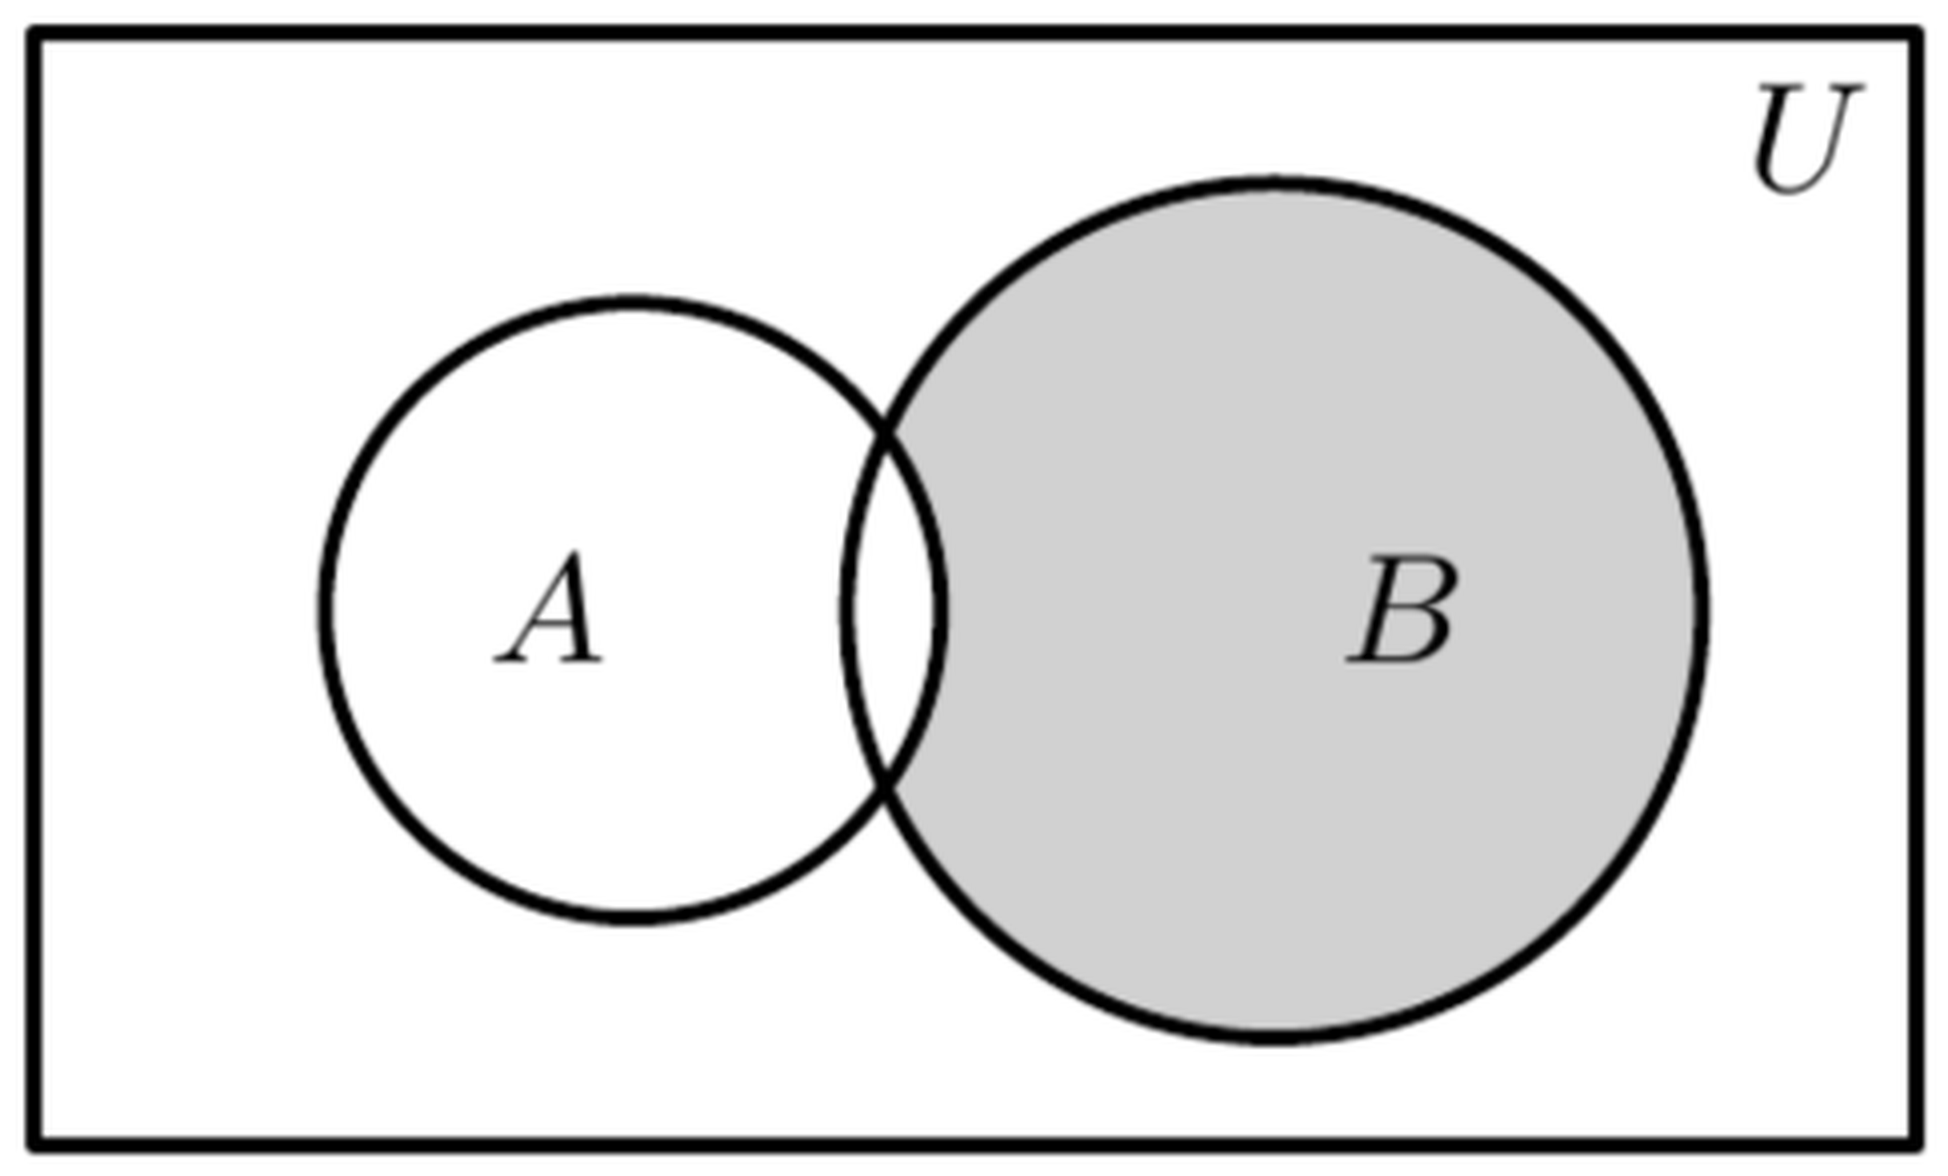
\includegraphics[width=0.38\textwidth]{figures/gao160_q4.png}
\end{center}

\ifanswer
\solbegin
\step{阴影部分表示 $B\cap\overline{A}=\{1,2\}$.}
\solend
\fi

% === Q5 === "图像"（有亻）照录；解析 1 行
\item 已知常数 $a>0$ 且 $a\ne1$，假设无论 $a$ 取何值，函数 $y=\log_a(5x-9)-4$ 的图像恒过一个定点，则这个定点的坐标为\blankline[4.4em].

\ifanswer
\solbegin
\step{$5x-9=1\Rightarrow x=2$，此时 $y=\log_a 1-4=-4$，定点为 $(2,-4)$.}
\solend
\fi

% === Q6 === 解析 2 行
\item 不等式 $(1-2x)^{\frac{3}{4}}>x^{\frac{3}{4}}$ 的解集为\blankline[4.4em].

\ifanswer
\solbegin
\step{定义域为 $\left[0,\dfrac{1}{2}\right]$，由幂函数的单调性，原不等式等价于 $1-2x>x$，}
\step{得 $0\leqslant x<\dfrac{1}{3}$，故解集为 $\left[0,\dfrac{1}{3}\right)$.}
\solend
\fi

% === Q7 === 绝对值 \lvert…\rvert；解析 2 行（跨 01—02 页）
\item 已知不等式 $\lvert x+3\rvert+\lvert x-2\rvert\geqslant 5$，当其等号成立时，$x$ 的取值范围是\blankline[4.4em].

\ifanswer
\solbegin
\step{$\lvert x+3\rvert+\lvert x-2\rvert=\lvert x+3\rvert+\lvert 2-x\rvert\geqslant\lvert(x+3)+(2-x)\rvert=5$，}
\step{等号成立当且仅当 $(x+3)(2-x)\geqslant0$，即 $x\in[-3,2]$.}
\solend
\fi

% === Q8 === 解析 4 行
\item 已知函数 $f(x)=\lvert\log_2 x\rvert$，若方程 $f(x)-t=0$ 有两个不同的实数根 $x_1,x_2$，则 $x_1+x_2$ 的取值范围是\blankline[4.4em].

\ifanswer
\solbegin
\step{方程有两个不同实根，必有 $t>0$，两根为 $2^t,2^{-t}$，}
\step{所以 $x_1+x_2=2^t+2^{-t}>2$（等号仅在 $t=0$ 时成立）.}
\step{任取 $s>2$，令 $a=\dfrac{s+\sqrt{s^2-4}}{2}>1$，取 $t=\log_2 a>0$，则 $x_1+x_2=a+\dfrac{1}{a}=s$，}
\step{所以取值范围为 $(2,+\infty)$.}
\solend
\fi

% === Q9 === 中文弯引号、\R、绝对值 \lvert…\rvert；解析 4 行
\item 已知 $a\in\R$，$b\in\R$，$p:\dfrac{1}{\lvert a\rvert}>\dfrac{1}{\lvert b\rvert}$，$q:\dfrac{1}{a}>\dfrac{1}{b}$，则 $p$ 是 $q$\blankline[4.4em]条件（用“充分非必要”、“必要非充分”、“充要”或“既非充分又非必要”填空）.

\ifanswer
\solbegin
\step{由 $p$、$q$ 中的分式有意义，$a\ne0$ 且 $b\ne0$.}
\step{当 $a=-1,b=-2$ 时，$p$ 成立而 $q$ 不成立，故 $p$ 不是 $q$ 的充分条件.}
\step{当 $a=1,b=-1$ 时，$q$ 成立而 $p$ 不成立，故 $p$ 不是 $q$ 的必要条件.}
\step{故 $p$ 是 $q$ 的充分非必要条件.}
\solend
\fi

% === Q10 === 解析 3 行；其后独立【注】按语 5 行（见头注 ② ⑯、⑤ 1）
\item 已知常数 $a>0$，函数 $y=\dfrac{2^x}{2^x+ax}$ 的图像经过点 $P\left(p,\dfrac{5}{6}\right)$、$Q\left(q,\dfrac{1}{6}\right)$，若 $2^{p+q}=3pq$，则 $a=$\blankline[4.4em].

\ifanswer
\solbegin
\step{由 $\dfrac{2^p}{2^p+ap}=\dfrac{5}{6}$ 得 $2^p=5ap$；由 $\dfrac{2^q}{2^q+aq}=\dfrac{1}{6}$ 得 $2^q=\dfrac{aq}{5}$.}
\step{$2^p>0$，$2^q>0$，$a>0$，得 $p>0$，$q>0$.}
\step{两式相乘得 $2^{p+q}=a^2pq$，又 $2^{p+q}=3pq$ 且 $pq\ne0$，故 $a^2=3$，$a=\sqrt{3}$.}
\solend
% 【注】按语（讲评版编者按，5 个印刷行，仅答案版出，不属于任何题的【解析】）
\stepm{【注】}{按原卷数据严格推敲，点 $Q$ 其实不存在：$a=\sqrt{3}$ 时 $2^q=\dfrac{\sqrt{3}}{5}q<q$；而当 $q>0$}
\step{时，取非负整数 $n$ 使 $n\leqslant q<n+1$，由 $2^{k+1}=2^k+2^k\geqslant2^k+1$ 逐次推得 $2^n\geqslant n+1$，于是}
\step{$2^q\geqslant2^n\geqslant n+1>q$，矛盾. 所以题设条件互相矛盾，严格说本题无解；$\sqrt{3}$ 是由题给关}
\step{系直接推出的值，按命题意图作为答案. 原卷数据疑似有误（同型常见题为 $P\left(p,\dfrac{6}{5}\right)$、}
\step{$Q\left(q,-\dfrac{1}{5}\right)$、$2^{p+q}=36pq$，得 $a=6$）.}% 见头注 ⑤ 1，照录未改
\fi

% === Q11 === 纳皮尔对数材料题；\Z、大数；解析 6 行
\item 17 世纪初，约翰·纳皮尔为了简化计算而发明了对数. 对数的发明是数学史上的重大事件，恩格斯曾经把笛卡尔的坐标系、纳皮尔的对数、牛顿和莱布尼兹的微积分共同称为 17 世纪的三大数学发明. 我们知道，任何一个正实数 $N$ 可以表示成 $N=a\times10^n$ ($1\leqslant a<10,n\in\Z$) 的形式，这便是科学记数法，若两边取常用对数，有 $\lg N=n+\lg a$，则可以估计 $3^{2026}$ 的最高位上的数值为\blankline[4.4em].

\ifanswer
\solbegin
\step{设 $3^{2026}=a\times10^n$ ($1\leqslant a<10,n\in\Z$)，则 $2026\lg 3=n+\lg a$.}
\step{用 $\lg 3\approx 0.4771$ 粗估，得 $2026\lg 3\approx 966.60$.}
\step{为核验误差，用 $0.47712<\lg 3<0.47713$，}
\step{得 $966.64512<2026\lg 3<966.66538$，因此 $n=966$.}
\step{于是 $\lg 4\approx 0.60206<0.64512<\lg a<0.66538<\lg 5\approx 0.69897$，}
\step{所以 $4<a<5$，最高位为 4，估算误差不影响结论.}
\solend
\fi

% === Q12 === 自定义"性质 P"；文本圈数字①②③；解析 19 行（跨 03—05 页）
\item 对于数集 $X=\{-1,x_1,x_2,x_3,\cdots,x_n\}$，其中 $0<x_1<x_2<x_3<\cdots<x_n$，$n\geqslant2$，定义点集 $Y=\{(s,t)\mid s\in X,t\in X\}$，若对于任意 $(s_1,t_1)\in Y$，存在 $(s_2,t_2)\in Y$，使得 $s_1s_2+t_1t_2=0$，则称集合 $X$ 具有性质 $P$. 则下列命题中为真命题的是\blankline[4.4em].

① $X=\{-1,1,2\}$ 具有性质 $P$；②若集合 $X$ 具有性质 $P$，则 $1\in X$；

③集合 $X$ 具有性质 $P$，若 $x_1=\dfrac{1}{2}$，则 $x_n=2$.

\ifanswer
\solbegin
\step{因为 $X=\{-1,1,2\}$，}
\step{所以 $Y=\{(-1,-1),(1,1),(2,2),(-1,1),(-1,2),(1,-1),(1,2),(2,-1),(2,1)\}$，}
\step{由集合 $X$ 具有性质 $P$ 的定义，对于任意 $(s,t)\in Y$，}
\step{若 $s>0$，$t>0$，则 $s=t$ 或 $(s,t)=(1,2)$ 或 $(s,t)=(2,1)$，}
\step{若 $s=t$，取 $s_2=-1$，$t_2=-1$，则 $ss_2+tt_2=0$；}
\step{若 $(s,t)=(1,2)$，取 $s_2=2$，$t_2=-1$，则 $ss_2+tt_2=0$；}
\step{若 $(s,t)=(2,1)$，取 $s_2=-1$，$t_2=2$，则 $ss_2+tt_2=0$；}
\step{若 $s$、$t$ 有一个为负数，则 $s=-1$ 或 $t=-1$，}
\step{若 $s=-1$，则取 $s_2=t$，$t_2=1$，则 $ss_2+tt_2=0$；}
\step{若 $t=-1$，则取 $s_2=1$，$t_2=s$，则 $ss_2+tt_2=0$；故①正确；}
\step{对于任意 $(s_1,t_1)\in Y$，存在 $(s_2,t_2)\in Y$，使得 $s_1s_2+t_1t_2=0$，}
\step{取 $(x_1,x_1)\in Y$，存在 $(x_p,x_q)$ 使得 $x_1x_p+x_1x_q=0$，所以 $x_p+x_q=0$，}
\step{不妨设 $x_p=1$，$x_q=-1$，所以若集合 $X$ 具有性质 $P$，则 $1\in X$，故②正确；}
\step{③假设 $x_n>1$，令 $s_1=\dfrac{1}{2},t_1=x_n$，则存在 $s$、$t\in X$ 使得 $\dfrac{1}{2}s+tx_n=0$，}
\step{同②得 $s$、$t$ 中必有一个数为 $-1$，}
\step{若 $s=-1$，则 $tx_n=\dfrac{1}{2}$，于是 $t=\dfrac{1}{2x_n}<\dfrac{1}{2}=x_1$，矛盾，}
\step{若 $t=-1$，则 $\dfrac{1}{2}s=x_n\cdot(-1)$，于是 $s=2x_n>x_n$，也矛盾，}% 原卷如此（与结论符号不自洽），照录未改，见头注 ⑤ 2
\step{所以 $x_n\leqslant1$，又由②得 $1\in X$，所以 $x_n\geqslant1$，所以 $x_n=1$，故③错误，}
\step{故真命题是①②.}
\solend
\fi

\end{enumerate}

% 答案版里填空解析把页排满，节标题会落到页末、与第 13 题分家（切页审计 B 类）；
% 守卫放 \bigsec 之前，连节标题一起量页高（高一157 成例）
\needvspace{7cm}
\bigsec{二、选择题}

\begin{enumerate}
\setcounter{enumi}{12}

% === Q13 === "图像"照录；解析 1 行，故选 $B$
\item 下列函数中，图像与函数 $y=3^x$ 图像关于 $y$ 轴对称的是\mbox{（\quad）}

\keepwithprev
A. $y=x^3$\qquad B. $y=\left(\dfrac{1}{3}\right)^x$\qquad C. $y=-3^x$\qquad D. $y=\log_3 x$

\ifanswer
\solbegin
\step{将 $x$ 换为 $-x$，得对称图像对应的函数为 $y=3^{-x}=\left(\dfrac{1}{3}\right)^x$，故选 $B$.}
\solend
\fi

% === Q14 === 中文弯引号；解析 2 行（跨 05 页上下），故选 $B$
\item 命题“存在 $x\in(1,+\infty)$，使得 $f(x)>0$”的否定形式为\mbox{（\quad）}

\keepwithprev
A. 不存在 $x\in(-\infty,1]$，使得 $f(x)>0$\qquad B. 对任意 $x\in(1,+\infty)$，有 $f(x)\leqslant0$

C. 对任意 $x\in(-\infty,1]$，有 $f(x)\leqslant0$\qquad D. 存在 $x\in(1,+\infty)$，使得 $f(x)\leqslant0$

\ifanswer
\solbegin
\step{将“存在”改为“对任意”，$x$ 的范围不变，并将 $f(x)>0$ 否定为 $f(x)\leqslant0$，}
\step{故选 $B$.}
\solend
\fi

% === Q15 === \R；四选项两行；解析 3 行，故选 $D$
\item 设 $a>0$，$s\in\R$. 下列各项中，能推出 $a^s>a$ 的一项是\mbox{（\quad）}

\keepwithprev
A. $a>1$，且 $s>0$\qquad B. $a>1$，且 $s<0$

C. $0<a<1$，且 $s>0$\qquad D. $0<a<1$，且 $s<0$

\ifanswer
\solbegin
\step{当 $a>1$ 时，$a^s>a\Leftrightarrow s>1$，A、B 均不能保证.}
\step{当 $0<a<1$ 时，$a^s>a\Leftrightarrow s<1$，C 不能保证，D 中 $s<0<1$，满足要求；}
\step{故选 $D$.}
\solend
\fi

% === Q16 === 题目配图（三版都出）；几何符号 \triangle ABC；解析 3 行，故选 $C$
\needvspace{8cm}
\item 数学说明的方法多种多样，其中利用图形说明就是一种重要方法. 如图所示，在等腰直角三角形 $\triangle ABC$ 中，点 $O$ 为斜边 $AB$ 的中点，点 $D$ 为斜边 $AB$ 上异于顶点的一个动点，设 $AD=a$，$BD=b$，则可用该图形能说明的不等式为\mbox{（\quad）}

\begin{center}
% Q16 等腰直角三角形 ABC 图（C/A/O/D/B 标注）取 05 页右下，去粉色水印、去色、3× LANCZOS 放大；三版都出
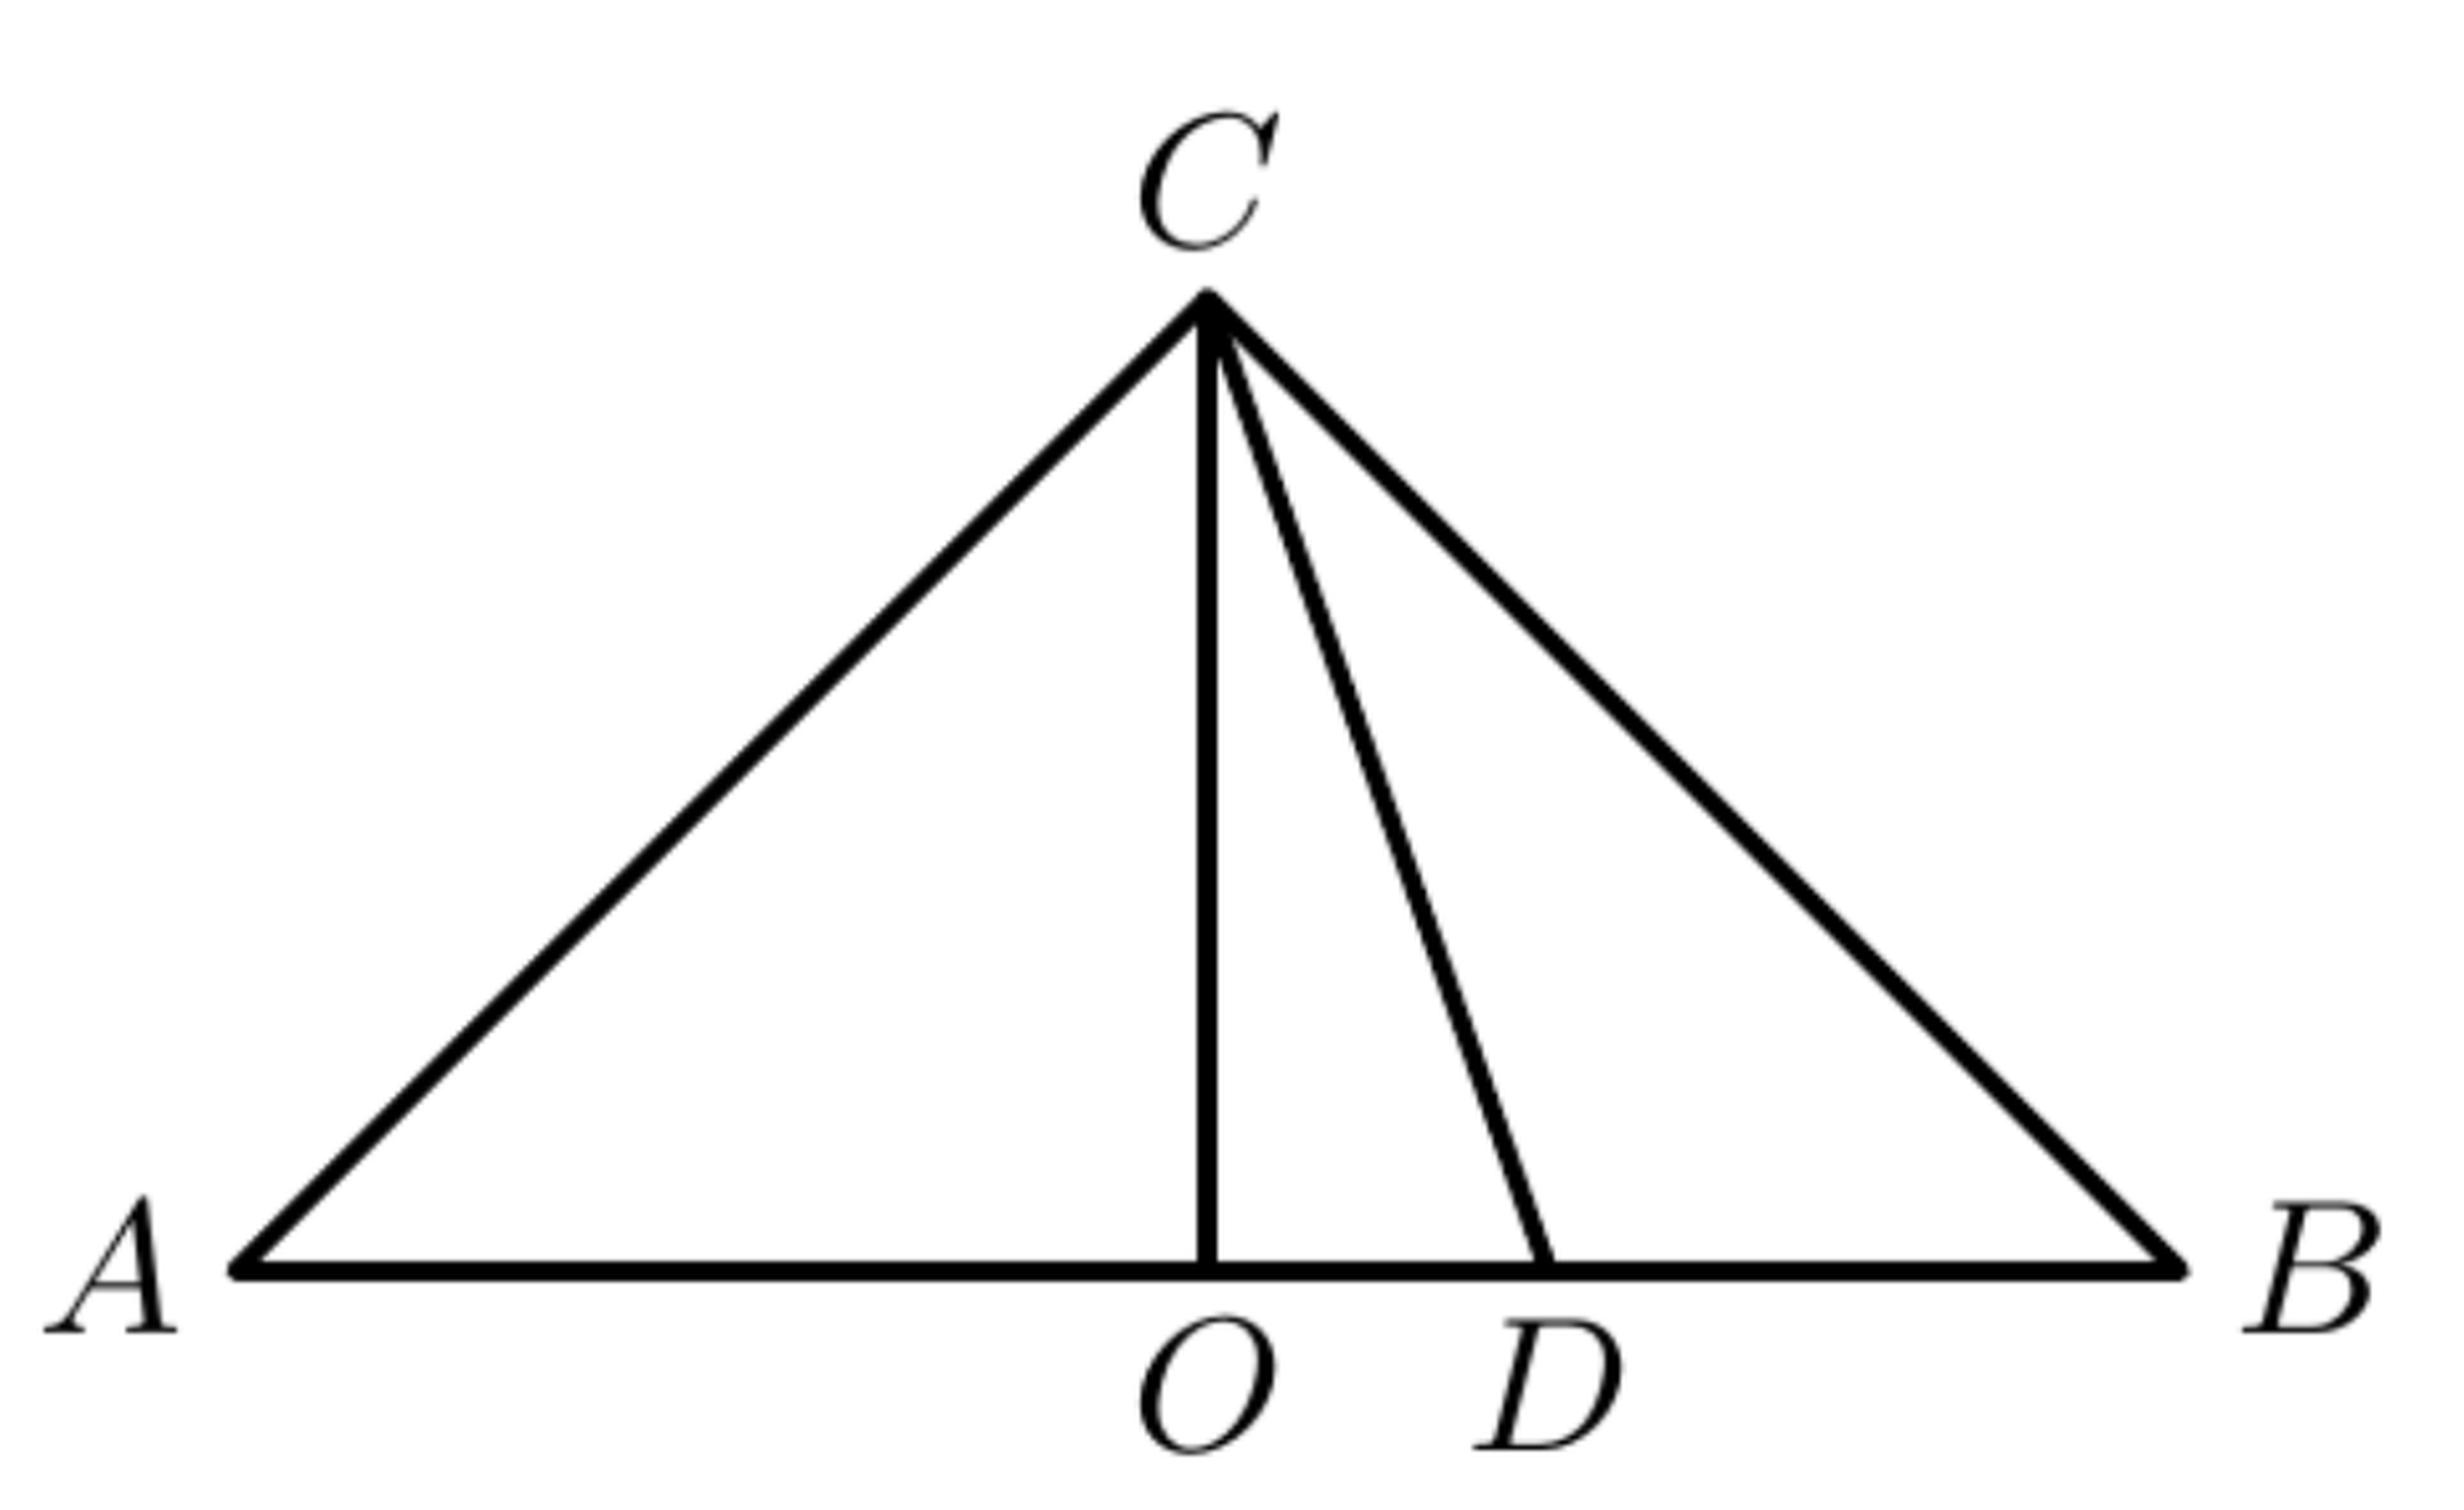
\includegraphics[width=0.34\textwidth]{figures/gao160_q16.png}
\end{center}

\keepwithprev
A. $\dfrac{a+b}{2}\geqslant\sqrt{ab}$ ($a>0,b>0$)\qquad B. $a^2+b^2\geqslant2\sqrt{ab}$ ($a>0,b>0$)

C. $\dfrac{a+b}{2}\leqslant\sqrt{\dfrac{a^2+b^2}{2}}$ ($a>0,b>0$)\qquad D. $\dfrac{2ab}{a+b}\leqslant\sqrt{ab}$ ($a>0,b>0$)

\ifanswer
\solbegin
\step{$CO=AO=\dfrac{a+b}{2},OD=\left\lvert a-\dfrac{a+b}{2}\right\rvert=\dfrac{\lvert a-b\rvert}{2}$，}
\step{$CD=\sqrt{CO^2+OD^2}=\sqrt{\dfrac{a^2+b^2}{2}}\geqslant CO=\dfrac{a+b}{2}$，}
\step{等号当且仅当 $a=b$ 时成立，故选 $C$.}
\solend
\fi

\end{enumerate}

\bigsec{三、解答题}

\begin{enumerate}
\setcounter{enumi}{16}

% === Q17 === cases 块算一行；判别式印等腰偏高三角 \Delta；解析 7 行
\item 已知幂函数 $f(x)=(m^2-2m-2)x^{m-1}$ 在 $(0,+\infty)$ 上是严格增函数.

(1) 求 $m$ 的值；

(2) 若关于 $x$ 的方程 $f(x)=(t+1)x-t^2$ 有两个不相等的正实根，求实数 $t$ 的取值范围.

\ifanswer
\solbegin
\step{(1) 幂函数的系数为 1，因此 $m^2-2m-2=1\Leftrightarrow(m-3)(m+1)=0$，}
\step{解得 $m=3$ 或 $m=-1$.}
\step{由 $f(x)$ 在 $(0,+\infty)$ 上严格递增，得 $m-1>0$，所以 $m=3$，}
\step{此时 $f(x)=x^2$.}
\step{(2) 原方程化为 $x^2-(t+1)x+t^2=0$，}
\step{方程有两个不相等的正实根，则 $\begin{cases}\Delta=(t+1)^2-4t^2=(1-t)(3t+1)>0\\t+1>0\\t^2>0\end{cases}$，}% 判别式原卷印等腰偏高三角 \Delta，照录
\step{得 $t\in\left(-\dfrac{1}{3},0\right)\cup(0,1)$.}
\solend
\fi

% === Q18 === 补集上划线 \overline{A}、\subseteq 带下划线、\varnothing；解析 8 行
\item 已知集合 $A=\{x\mid\lvert x-a\rvert<a-3\}$，$B=\left\{x\mid\dfrac{x+1}{x-2}\geqslant2\right\}$.

(1) 若 $a=5$，求 $\overline{A}\cap B$；

(2) 若 $A\cap B=A$，求实数 $a$ 的取值范围.

\ifanswer
\solbegin
\step{(1) $\dfrac{x+1}{x-2}\geqslant2\Leftrightarrow\dfrac{5-x}{x-2}\geqslant0\Leftrightarrow2<x\leqslant5,B=(2,5]$，}
\step{当 $a=5$ 时，$A=\{x\mid\lvert x-5\rvert<2\}=(3,7)$，于是 $\overline{A}=(-\infty,3]\cup[7,+\infty)$，}
\step{因此 $\overline{A}\cap B=(2,3]$.}
\step{(2) $A\cap B=A$ 等价于 $A\subseteq B$.}
\step{当 $a\leqslant3$ 时，$a-3\leqslant0$，$A=\varnothing$，满足条件.}
\step{当 $a>3$ 时，$\lvert x-a\rvert<a-3\Leftrightarrow3<x<2a-3,A=(3,2a-3)$，}
\step{此时 $A\subseteq B=(2,5]$ 等价于 $2a-3\leqslant5$，即 $a\leqslant4$，结合 $a>3$ 得 $3<a\leqslant4$.}
\step{合并两种情形，实数 $a$ 的取值范围为 $(-\infty,4]$.}
\solend
\fi

% === Q19 === 数据表 tabular 重排（高一130 成例）；cases 块算一行；解析 6 行
\item 作为我国最高水平的综合性运动会，全运会汇聚了国内顶尖体育健儿，某代表队从第 8 届全运会开始登上赛场，且参赛运动员人数逐年递增. 设 $t$ 为该代表队参赛后经过的届数，即第 8 届为 $t=0$，第 9 届为 $t=1$，以此类推. 经过 $t$ 届，运动员人数为 $y$ 人，具体数据如下：

\begin{center}
\begin{tabular}{cccccc}
$t$ & 0 & 1 & 2 & 3 & 4 \\
\hline
届数 & 8 & 9 & 10 & 11 & 12 \\
运动员人数（$y$ 人） & 4 & 11 & 25 & 53 & 109
\end{tabular}
\end{center}

(1) 现有以下两种函数模型：① $y=a\cdot b^t+c$ ($a>0,b>1$)；② $y=\log_a(t+b)+c$ ($b>0,a>1$). 请根据上表中运动员人数的增长规律，选出你认为符合的函数模型（不用说明理由），并利用表中前 3 组数据求出相应的函数解析式；

(2) 若参赛运动员人数按照 (1) 中求得的模型继续增长，在第几届全运会时，该代表队运动员人数将会首次超过 1000 人？

\ifanswer
\solbegin
\step{(1) 选模型①，将前 3 组数据代入，得 $\begin{cases}a+c=4\\ab+c=11\\ab^2+c=25\end{cases}$，}% 原卷印"选模型①"（圈数字①），OCR 误作"四"，照录①，见头注 ⑤ 3
\step{相邻两式相减，得 $a(b-1)=7$，$ab(b-1)=14$，}
\step{两式相除得 $b=2$，进而 $a=7$，$c=-3$，所求函数解析式为 $y=7\cdot2^t-3$.}
\step{(2) $y=7\cdot2^t-3$ 随 $t$ 的增大而增大，且 $t=7$ 时，$y=893<1000$；}
\step{$t=8$ 时，$y=1789>1000$，}
\step{$t$ 为非负整数，首次超过 1000 人时 $t=8$，对应第 $8+8=16$ 届全运会.}
\solend
\fi

% === Q20 === 解析 12 行（跨 08—09 页）
\item 已知函数 $f(x)=\log_a(a-a^x)$.

(1) 求该函数的定义域；

(2) 若 $a>1$，试判断关于 $x$ 的方程 $f(x)=2$ 是否有实数解，并说明理由；

(3) 若当 $x\in(-\infty,0]$ 时，关于 $x$ 的不等式 $f(x)\geqslant-1$ 恒成立，求实数 $a$ 的取值范围.

\ifanswer
\solbegin
\step{(1) 对数的底数须满足 $a>0$ 且 $a\ne1$，真数须满足 $a-a^x>0$，即 $a^x<a^1$.}% 原卷印 $a^1$，照录未化简，见头注 ⑤ 4
\step{当 $a>1$ 时，$x<1$，定义域为 $(-\infty,1)$.}
\step{当 $0<a<1$ 时，$x>1$，定义域为 $(1,+\infty)$.}
\step{(2) 当 $a>1$ 时，若 $f(x)=2$，则 $a-a^x=a^2\Rightarrow a^x=a(1-a)<0$，}
\step{这与 $a^x>0$ 矛盾，因此方程无实数解.}
\step{(3) 不等式在 $(-\infty,0]$ 上恒成立，须先保证该区间包含于函数的定义域，}
\step{由 (1) 得 $a>1$.}
\step{当 $x\leqslant0$ 时，$0<a^x\leqslant1$，所以 $a-a^x\geqslant a-1>0$.}
\step{由对数函数的单调性，$f(x)=\log_a(a-a^x)\geqslant\log_a(a-1)=f(0)$，}
\step{等号当且仅当 $x=0$ 时成立，}
\step{因此所求条件等价于 $\log_a(a-1)\geqslant-1\Leftrightarrow a-1\geqslant\dfrac{1}{a}\Leftrightarrow a^2-a-1\geqslant0$，}
\step{结合 $a>1$，得 $a\in\left[\dfrac{1+\sqrt{5}}{2},+\infty\right)$.}
\solend
\fi

% === Q21 === "和积平衡集"定义证明题；\N；解析 18 行（跨 09—10 页）
\item 已知有限集 $A=\{a_1,a_2,\cdots,a_n\}$ ($n\geqslant2,n\in\N$)，如果 $A$ 中元素 $a_i$ ($i=1,2,3,\cdots,n$) 满足 $a_1+a_2+a_3+\cdots+a_n=a_1\times a_2\times\cdots\times a_n$，就称 $A$ 为“和积平衡集”.

(1) 分别判断集合 $A=\{1,2,3,4\}$，$B=\{4+2\sqrt{2},4-2\sqrt{2}\}$ 是否为“和积平衡集”；

(2) 已知 $a_1$、$a_2$ 是两个不同的正数，且 $\{a_1,a_2\}$ 是“和积平衡集”，请用反证法证明：$a_1$、$a_2$ 至少有一个大于 2；

(3) 若 $a_i\geqslant1$，且 $a_i\in\N$，求所有符合条件的“和积平衡集”.

\ifanswer
\solbegin
\step{(1) 因为 $1+2+3+4=10\ne24=1\times2\times3\times4$，所以 $A$ 不是“和积平衡集”.}
\step{因为 $(4+2\sqrt{2})+(4-2\sqrt{2})=8=(4+2\sqrt{2})(4-2\sqrt{2})$，}
\step{所以 $B$ 是“和积平衡集”.}
\step{(2) 假设 $a_1$、$a_2$ 都不大于 2，则 $\dfrac{1}{a_1}\geqslant\dfrac{1}{2},\dfrac{1}{a_2}\geqslant\dfrac{1}{2}$，}
\step{由于 $a_1\ne a_2$，上述两个不等式至少有一个严格成立.}
\step{而 $a_1+a_2=a_1a_2$，两边除以 $a_1a_2>0$，得 $1=\dfrac{1}{a_1}+\dfrac{1}{a_2}>\dfrac{1}{2}+\dfrac{1}{2}=1$，矛盾，}
\step{所以 $a_1$、$a_2$ 至少有一个大于 2.}
\step{(3) 不妨设 $a_1<a_2<\cdots<a_n$，由各元素均为正整数，得 $a_i\geqslant i$.}
\step{若 $n\geqslant4$，因其余因子均不小于 1，}
\step{有 $a_1a_2\cdots a_n\geqslant a_2a_{n-1}a_n\geqslant2(n-1)a_n>na_n>a_1+a_2+\cdots+a_n$，}
\step{与和积平衡条件矛盾，因此只需讨论 $n=2,3$.}
\step{当 $n=2$ 时，$a_1+a_2=a_1a_2\Leftrightarrow(a_1-1)(a_2-1)=1$，}
\step{两个因子均为非负整数，只能有 $a_1=a_2=2$，与元素互不相同矛盾.}
\step{当 $n=3$ 时，若 $a_1\geqslant2$，则 $a_2\geqslant3$，从而 $a_1a_2a_3\geqslant6a_3>3a_3>a_1+a_2+a_3$，}
\step{矛盾，因此 $a_1=1$.}
\step{此时 $1+a_2+a_3=a_2a_3\Leftrightarrow(a_2-1)(a_3-1)=2$，}
\step{由 $1\leqslant a_2-1<a_3-1$，得 $a_2-1=1$、$a_3-1=2$，即 $a_2=2$、$a_3=3$.}
\step{检验 $1+2+3=1\times2\times3=6$，所求集合为 $\{1,2,3\}$.}
\solend
\fi

\end{enumerate}

\end{document}
"
%
% ① 原始材料：微信公众号"魔都数学加油站"文章，连载"27学年高一160"，原卷卷面标题
% "2026-2027 年奉贤中学高一上期中"（卷面未印副标题、未印连载号）。
% 正文为 10 张 PNG 页（01/04/10 为 2560×3620，02/03/05/06/07/08/09 为
% 4762×6735，同一篇各页分辨率混排，逐页按各自分辨率裁图核对）。
% 体例：讲评版——填空 3—12（10 题）、选择 13—16（4 题）、解答 17—21（5 题），
% 共 19 题，自第 3 题起编（1、2 未印在本篇）；19 题逐题印【解析】，无只印【答案】
% 的题；四道选择题答案在解析末句"故选 $B$/$B$/$D$/$C$"，题干括号
% \mbox{（\quad）} 留空、不另提 \ans{}。题目、答案、解析均据原图转录；卷面粉红色
% 水印"魔都数学加油站"及公众号页脚未录入。
% 全卷插图清单（逐页通读 10 页确认）：2 幅，均为题目配图、三版都出——
%   · Q4 韦恩图（01 页右侧：矩形全集 U、两圆 A/B、阴影部分 B∩上划线 A、
%     标注 U/A/B），裁 figures/gao160_q4.png；
%   · Q16 等腰直角三角形 ABC 图（05 页右下：C 顶点、A/O/D/B 共线底边、
%     CO 与 CD 两条线段），裁 figures/gao160_q16.png；
%   两图均取原卷截图 3—4× LANCZOS 放大、去粉色水印、转灰度、autocontrast；
%   Q4 图左侧题干残字"示"、Q16 图左侧题干残字均已裁白。
%   Q19 有一张 3 行数据表（t／届数／运动员人数（y 人），t=0..4），按全稿
%   成例（高一130）用 tabular 重排，不做成 png；其余各页无题目配图、
%   无解析内配图、无其它表格、无"如图"处。
%
% 卷首标题：原卷印作"2026-2027 年奉贤中学高一上期中"，年份区间按全稿惯例排 en dash；
% 原卷卷面未印副标题，本稿按同期中卷知识模块口径补出"集合与常用逻辑用语、不等式、函数"。
%
% ② 与原卷的排版差异／照录项清单：
%   ① 原文从第 3 题起，本稿保留原题号；共 19 题三节，解答题 5 题到 21；
%      三节各自一个 enumerate + \setcounter{enumi}{2}/{12}/{16}（不贯穿），
%      用 \examtitlest[3] 起手；
%   ② 混合体例说明：19 题全印【解析】、用 \solbegin…\solend，无只印【答案】
%      或答案印括号内的题；四道选择题答案在解析末句"故选 $B$/$B$/$D$/$C$"
%      （逐个放大复核）、括号 \mbox{（\quad）} 留空、不另提 \ans{}；答案版
%      【答案】/【解析】标记数 = 19 = 全卷题数（0 个 \ans ＋ 19 个 \solbegin）；
%   ③ 原卷卷面未印副标题，本稿按知识模块口径补出；
%   ④ 原卷填空横线按全稿惯例排 \blankline[4.4em]；选择题括号排 \mbox{（\quad）}、
%      四道选择题的选项段前按惯例各加 \keepwithprev；解答题不留作答区、不加
%      \anspace（原卷为讲评版，109—113 起全稿不用 \anspace）；
%   ⑤ 数集归一：Q4"$U=\Z$"、Q9"$a\in\R$，$b\in\R$"、Q11"$n\in\Z$"、
%      Q15"$s\in\R$"、Q21"$n\in\N$""$a_i\in\N$"原卷印正体粗体 Z/R/N，
%      按全稿惯例归一 \Z／\R／\N；集合描述竖线排 \mid（Q3、Q4、Q12、
%      Q18、Q21）；空集 \varnothing（Q18 解析 (2)）；补集照原卷上划线排
%      \overline{A}（Q4 解析、Q18 (1) 题干与解析）；子集符号 Q18 两处
%      "$A\subseteq B$"印带下划线 ⊆、照录 \subseteq；
%   ⑥ 绝对值排 \lvert…\rvert（Q7、Q8 题干与解析、Q9 题干、Q16 解析、
%      Q18 题干与解析），Q16 解析的 \left\lvert…\right\rvert 与 \lvert…\rvert
%      均在同一 $…$ 组内配对平衡；
%   ⑦ 判别式两形混用逐处照录不统一（放大逐处确认）：Q3 解析
%      "$\triangle=1^2-4a\times\frac{1}{4}=0$"原卷印扁等边三角、照录
%      \triangle；Q17 解析 cases 块"$\Delta=(t+1)^2-4t^2=(1-t)(3t+1)>0$"
%      原卷印等腰偏高三角、照录 \Delta；Q16 题干几何符号"$\triangle ABC$"
%      按全稿几何三角形记号惯例归一 \triangle（参照 高一150／132 成例）；
%   ⑧ 不等号按全稿惯例排 \leqslant／\geqslant；中文弯引号照录：Q9 题干
%      "充分非必要""必要非充分""充要""既非充分又非必要"、Q14 题干
%      "存在 $x\in(1,+\infty)$，使得 $f(x)>0$"与解析"存在""对任意"、
%      Q21 题干与解析多处"和积平衡集"；注释里一律 ASCII 引号；
%   ⑨ 文本圈数字逐处照录：Q12 题干①②③、Q12 解析"故①正确""同②得"
%      "故②正确""③假设""故③错误""故真命题是①②"、Q19 题干①②与解析
%      "选模型①"，均为印刷圈数字（非 \textcircled、非数学模式）；
%   ⑩ 半角逗号在数学组之间是全稿惯例、非笔误，逐处照录（Q8"$2^t,2^{-t}$"、
%      Q9"$a=-1,b=-2$""$a=1,b=-1$"、Q11"$1\leqslant a<10,n\in\Z$"、
%      Q12"$s_1=\frac{1}{2},t_1=x_n$"、Q16 选项"$a>0,b>0$"与解析
%      "$CO=AO=\frac{a+b}{2},OD=...$"、Q18"$2<x\leqslant5,B=(2,5]$"
%      "$3<x<2a-3,A=(3,2a-3)$"、Q21"$n=2,3$"等）；行中全角逗号／顿号
%      照录（Q15 选项"$a>1$，且 $s>0$"、Q12 解析"$s$、$t$"、Q21 解析
%      "$a_1$、$a_2$"），顿号一律移出数学模式；
%   ⑪ "图像／图象"逐处照录：本卷 Q5"的图像恒过一个定点"、Q10"的图像经过点"、
%      Q13 题干两处"图像"与解析"对称图像对应的函数"均印"图像"（有亻）；
%      Q16 印"图形"（利用图形说明、该图形能说明），无"图象"用例；
%   ⑫ 复杂式照录别简化：Q3 $ax^2+x+\frac14=0$、Q5 $y=\log_a(5x-9)-4$、
%      Q6 $(1-2x)^{\frac34}>x^{\frac34}$ 与 $\left[0,\frac12\right]$、
%      Q8 $\frac{s+\sqrt{s^2-4}}{2}$、Q10 $y=\frac{2^x}{2^x+ax}$ 与
%      $\frac{2^p}{2^p+ap}=\frac56$、$\frac{2^q}{2^q+aq}=\frac16$、
%      Q11 $N=a\times10^n$ 与 $3^{2026}$、$2026\lg3\approx966.60$、
%      $966.64512<2026\lg3<966.66538$、Q12 $Y=\{(s,t)\mid s\in X,t\in X\}$
%      与 $\frac12 s+tx_n=0$、Q16 $\sqrt{\frac{a^2+b^2}{2}}$、
%      Q17 $x^2-(t+1)x+t^2=0$ 与 $\left(-\frac13,0\right)\cup(0,1)$、
%      Q18 $\frac{5-x}{x-2}\geqslant0$、Q19 $y=a\cdot b^t+c$ 与
%      $y=\log_a(t+b)+c$、$y=7\cdot2^t-3$、Q20 $f(x)=\log_a(a-a^x)$
%      与 $a^2-a-1\geqslant0$、$\left[\frac{1+\sqrt5}{2},+\infty\right)$、
%      Q21 $4+2\sqrt2$ 与 $(a_2-1)(a_3-1)=2$ 等；
%   ⑬ 子题标号 (1)(2)(3) 按全稿惯例排半角括号；行末／行中句点按全稿惯例
%      排 ASCII `.`（不是全角「．」）；cases 块整体算一个印刷行
%      （Q17 解析、Q19 解析 (1)）；
%   ⑭ 配图：Q4／Q16 题目配图（三版都出）放 \item 内题干之后 \begin{center}，
%      各用 \needvspace{8cm} 守卫把整块推走，**守卫放在 \item 之前**
%      （见 高一153 Q11/Q19 成例与切页审计 B 类坑）；
%   ⑮ 一条 \step = 原卷解析的一个印刷行；跨上下半页的重叠行只算一次
%      （Q4 解析、Q9 解析首行、Q11 解析首行、Q12 解析"若 $s=-1$…"一行、
%      Q18 解析"此时 $A\subseteq B=(2,5]$…"一行、Q20 (2) 题干、
%      Q21 解析"由 $1\leqslant a_2-1<a_3-1$…"一行）；原卷折行别合并；
%   ⑯ Q10 之后另有一整块【注】按语（03 页上半，5 个印刷行），是讲评版作者对
%      原卷数据自相矛盾的加注、不属于任何题的【解析】。本稿按 高一53
%      "注：…"成例放 Q10 的 \solend 之后、Q10 的 \fi 收尾之前：
%      **整块只保留 Q10 那一层外层 \ifanswer**（那个 \fi 就是 Q10 的收尾），
%      块内 \stepm{【注】}{首行} ＋ 4 条 \step 各自自带内层 \ifanswer…\fi
%      （\step／\stepm 宏内自带，源码里不手动再包一层 \ifanswer，
%      否则 题目溯源.py 的 strip_answers 非贪婪正则会错切）；
%      \stepm 第一参数直接用「【注】」作标签，与全稿 \ans 的【答案】、
%      \solbegin 的【解析】同性质，未加粗以外不另加任何样式；
%      5 行仅答案版出、不新增 \item、不影响溯源，头注 ③ 单列登记、
%      不计入 19 题逐题 \step 账；\stepm 把【注】排成加粗着色标签
%      （原卷为黑色加粗），此一处着色差异在此登记；
%   ⑰ 原卷用字照录：Q11"约翰·纳皮尔""莱布尼兹"（原卷作"兹"，非通行"茨"）、
%      "17 世纪的三大数学发明"；Q16"数学说明的方法""点 $D$ 为斜边 $AB$ 上
%      异于顶点的一个动点"；Q19"登上赛场""以此类推"；
%
% ③ 行数复核：一条 \step = 原卷解析的一个印刷行，cases 块作一个印刷行计。
%   逐题数（逐页核对定稿）：Q3：5；Q4：1；Q5：1；Q6：2；Q7：2；Q8：4；
%   Q9：4；Q10：3；Q11：6；Q12：19；Q13：1；Q14：2；Q15：3；Q16：3；
%   Q17：7；Q18：8；Q19：6；Q20：12；Q21：18。
%   合计 107 条 \step（19 题逐题印刷行账），与原卷逐题印刷行相等。
%   **本卷源码 \step 总数 = 19 题逐题合计 107 ＋ Q10 后独立【注】块 5 行
%   = 112 行**（其中 \step 111 条、\stepm 1 条；\stepm 与 4 条 \step 合为
%   【注】块 5 印刷行）。该 5 行不计入「逐题印刷行」账，也不是任何题的
%   【解析】，而是讲评版编者按语；主会话核验脚本按全文统计 \step 时总数会
%   较逐题账多 5，已与主会话对齐、属已知预期而非错误。
%   全卷 19 题均设 \solbegin…\solend，答案版【答案】/【解析】标记数
%   = 19 = 全卷题数。
%
% ④ 页码分布（供回原图复核）：
%   卷首标题＋"一、填空题"＋Q3 题干＋解析 5 行＋Q4 题干＋韦恩图＋解析
%   1 行＋Q5 题干首行在 01 页上半；Q4 解析（重叠）＋Q5 题干续＋解析 1 行＋
%   Q6 题干＋解析 2 行＋Q7 题干＋解析首行在 01 页下半；Q7 解析末行＋
%   Q8 题干＋解析 4 行＋Q9 题干＋解析首行在 02 页上半；Q9 解析（重叠首行）
%   ＋余 3 行＋Q10 题干＋解析 3 行在 02 页下半；【注】按语 5 行＋Q11 题干＋
%   解析首行在 03 页上半；Q11 解析（重叠首行）＋余 5 行＋Q12 题干＋①②
%   在 03 页下半；Q12 ③＋解析前 9 行在 04 页上半；Q12 解析（重叠 2 行）
%   ＋余 8 行在 04 页下半；Q12 解析末 2 行＋"二、选择题"＋Q13 题干＋选项＋
%   解析 1 行＋Q14 题干＋选项＋解析首行在 05 页上半；Q14 解析末行＋
%   Q15 题干＋选项＋解析 3 行＋Q16 题干＋三角形图在 05 页下半；
%   Q16 选项＋解析 3 行＋"三、解答题"＋Q17 题干＋两问在 06 页上半；
%   Q17 解析 7 行在 06 页下半；Q18 题干＋两问＋解析前 7 行＋Q19 题干首行
%   在 07 页上半；Q18 解析末行（重叠）＋Q19 题干＋表格＋两问在 07 页下半；
%   Q19 解析 6 行＋Q20 题干＋(1)(2) 在 08 页上半；Q20 (2)(3) 题干（重叠）
%   ＋解析 8 行在 08 页下半；Q20 解析末 4 行＋Q21 题干＋(1)(2) 在 09 页
%   上半；Q21 (3)＋解析前 7 行在 09 页下半；Q21 解析 (3) 余 10 行在 10 页
%   上半；Q21 末行（重叠）＋"检验 $1+2+3=1\times2\times3=6$，所求集合为
%   $\{1,2,3\}$."在 10 页下半（此后仅水印、无正文）。本稿按题连排，
%   不丢行、不并折行；全卷末题为第 21 题，无附加题节。
%
% ⑤ 存疑照录（放大原图确认，照录未改、正文对应处另有 % 注）：
%   1. Q10【注】按语：讲评版作者据 $a=\sqrt3$ 时 $2^q=\frac{\sqrt3}{5}q<q$
%      与 $2^n\geqslant n+1$ 推出点 $Q$ 不存在、"严格说本题无解"，并注明
%      "原卷数据疑似有误（同型常见题为 $P(p,\frac65)$、$Q(q,-\frac15)$、
%      $2^{p+q}=36pq$，得 $a=6$）"；本稿照录全块、未删未改（见 ② ⑯）。
%   2. Q12 解析 (3) 末段"若 $t=-1$，则 $\frac{1}{2}s=x_n\cdot(-1)$，
%      于是 $s=2x_n>x_n$，也矛盾，"中，等式右端与紧随的结论符号不自洽
%      （按题意应为 $\frac12 s=x_n$ 或 $-\frac12 s=x_n\cdot(-1)$），逐页
%      放大 04 页确认原卷即如此印、无漏看的负号，照录未改，建议主会话
%      回 04 页再放大复核一次；
%   3. Q19 解析 (1) 印"选模型①"（圈数字①，题干只有①②两种模型）；
%      OCR 误作"选模型四"，放大 08 页确认是①、照录①；
%   4. Q20 解析 (1)"即 $a^x<a^1$"末项原卷印 $a^1$（非 $a$），照录未化简；
%   5. Q11 题干"莱布尼兹"原卷作"兹"（非通行"茨"）、"约翰·纳皮尔"用
%      间隔号·，均照录未改；
%   6. Q9 题干"则 $p$ 是 $q$___条件"与解析"故 $p$ 是 $q$ 的充分非必要条件"
%      句式略异，均照录；
%   7. Q19 解析 (1) 用"前 3 组数据"、题干表格列到 $t=4$，照录未补。
%
\documentclass[a4paper,11pt]{article}
\usepackage{common}

\begin{document}

\examtitlest[3]{2026--2027 年奉贤中学高一上期中}{集合与常用逻辑用语、不等式、函数}

\bigsec{一、填空题}

\begin{enumerate}
\setcounter{enumi}{2}

% === Q3 === 解析 5 行；判别式印扁等边三角 \triangle
\item 若集合 $A=\{x\mid ax^2+x+\dfrac{1}{4}=0\}$ 有且仅有两个子集，则实数 $a=$\blankline[4.4em].

\ifanswer
\solbegin
\step{若集合 $A=\{x\mid ax^2+x+\dfrac{1}{4}=0\}$ 有且仅有两个子集，}
\step{所以方程 $ax^2+x+\dfrac{1}{4}=0$ 只有一个实数根，}
\step{当 $a=0$ 时，方程化为 $x+\dfrac{1}{4}=0$，解得 $x=-\dfrac{1}{4}$，符合题意，}
\step{当 $a\ne0$ 时，则 $\triangle=1^2-4a\times\dfrac{1}{4}=0$，解得 $a=1$，}% 判别式原卷印扁等边三角 \triangle，照录
\step{综上所述，实数 $a=0$ 或 1.}
\solend
\fi

% === Q4 === 题目配图（三版都出）；\needvspace 守卫放 \item 之前；补集上划线 \overline{A}；解析 1 行
\needvspace{8cm}
\item 设全集 $U=\Z$，集合 $A=\{x\mid -3<x<1\}$，$B=\{-1,0,1,2\}$，用列举法表示图中阴影部分为\blankline[4.4em].

\begin{center}
% Q4 韦恩图（全集 U、A/B 两圆、阴影 B∩上划线 A）取 01 页右侧，去粉色水印、去色、4× LANCZOS 放大；三版都出
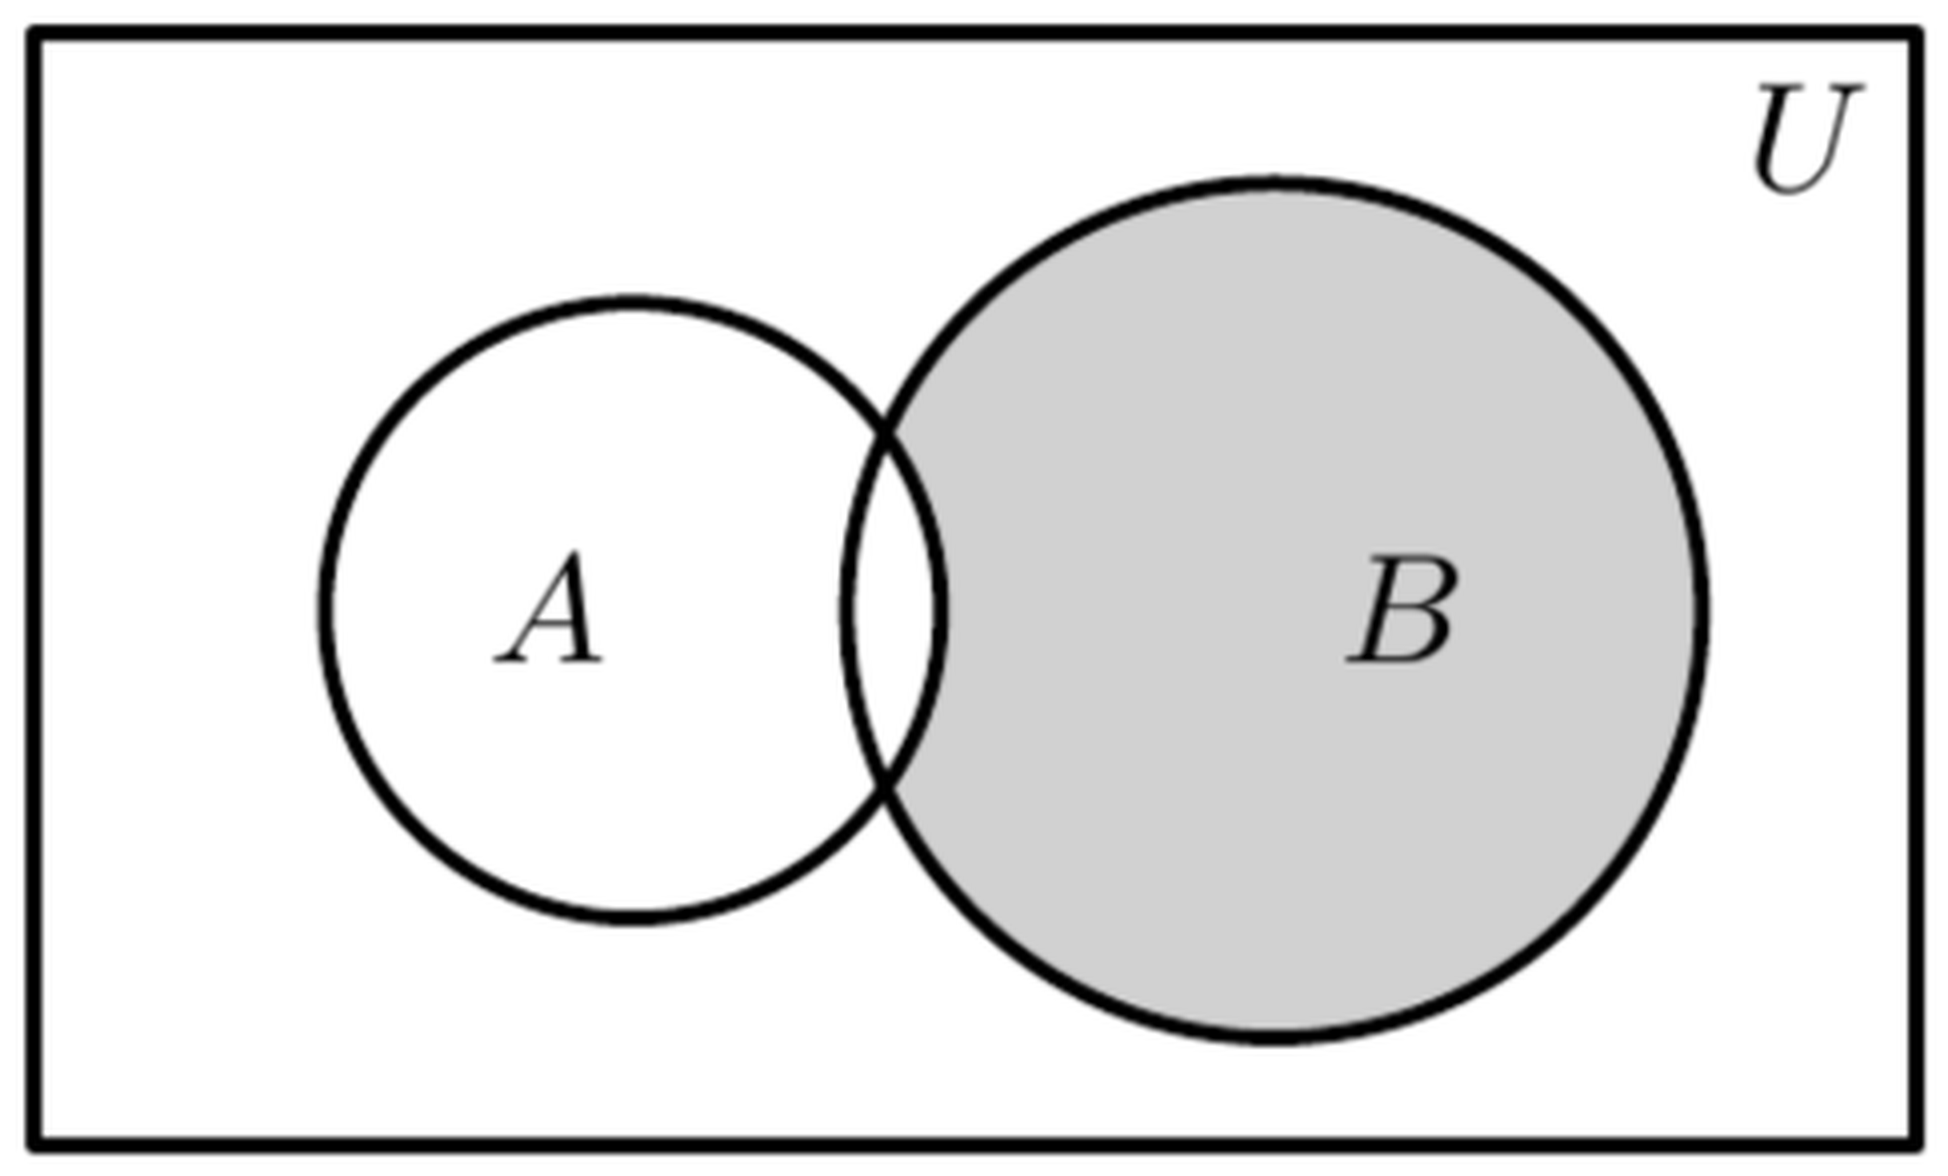
\includegraphics[width=0.38\textwidth]{figures/gao160_q4.png}
\end{center}

\ifanswer
\solbegin
\step{阴影部分表示 $B\cap\overline{A}=\{1,2\}$.}
\solend
\fi

% === Q5 === "图像"（有亻）照录；解析 1 行
\item 已知常数 $a>0$ 且 $a\ne1$，假设无论 $a$ 取何值，函数 $y=\log_a(5x-9)-4$ 的图像恒过一个定点，则这个定点的坐标为\blankline[4.4em].

\ifanswer
\solbegin
\step{$5x-9=1\Rightarrow x=2$，此时 $y=\log_a 1-4=-4$，定点为 $(2,-4)$.}
\solend
\fi

% === Q6 === 解析 2 行
\item 不等式 $(1-2x)^{\frac{3}{4}}>x^{\frac{3}{4}}$ 的解集为\blankline[4.4em].

\ifanswer
\solbegin
\step{定义域为 $\left[0,\dfrac{1}{2}\right]$，由幂函数的单调性，原不等式等价于 $1-2x>x$，}
\step{得 $0\leqslant x<\dfrac{1}{3}$，故解集为 $\left[0,\dfrac{1}{3}\right)$.}
\solend
\fi

% === Q7 === 绝对值 \lvert…\rvert；解析 2 行（跨 01—02 页）
\item 已知不等式 $\lvert x+3\rvert+\lvert x-2\rvert\geqslant 5$，当其等号成立时，$x$ 的取值范围是\blankline[4.4em].

\ifanswer
\solbegin
\step{$\lvert x+3\rvert+\lvert x-2\rvert=\lvert x+3\rvert+\lvert 2-x\rvert\geqslant\lvert(x+3)+(2-x)\rvert=5$，}
\step{等号成立当且仅当 $(x+3)(2-x)\geqslant0$，即 $x\in[-3,2]$.}
\solend
\fi

% === Q8 === 解析 4 行
\item 已知函数 $f(x)=\lvert\log_2 x\rvert$，若方程 $f(x)-t=0$ 有两个不同的实数根 $x_1,x_2$，则 $x_1+x_2$ 的取值范围是\blankline[4.4em].

\ifanswer
\solbegin
\step{方程有两个不同实根，必有 $t>0$，两根为 $2^t,2^{-t}$，}
\step{所以 $x_1+x_2=2^t+2^{-t}>2$（等号仅在 $t=0$ 时成立）.}
\step{任取 $s>2$，令 $a=\dfrac{s+\sqrt{s^2-4}}{2}>1$，取 $t=\log_2 a>0$，则 $x_1+x_2=a+\dfrac{1}{a}=s$，}
\step{所以取值范围为 $(2,+\infty)$.}
\solend
\fi

% === Q9 === 中文弯引号、\R、绝对值 \lvert…\rvert；解析 4 行
\item 已知 $a\in\R$，$b\in\R$，$p:\dfrac{1}{\lvert a\rvert}>\dfrac{1}{\lvert b\rvert}$，$q:\dfrac{1}{a}>\dfrac{1}{b}$，则 $p$ 是 $q$\blankline[4.4em]条件（用“充分非必要”、“必要非充分”、“充要”或“既非充分又非必要”填空）.

\ifanswer
\solbegin
\step{由 $p$、$q$ 中的分式有意义，$a\ne0$ 且 $b\ne0$.}
\step{当 $a=-1,b=-2$ 时，$p$ 成立而 $q$ 不成立，故 $p$ 不是 $q$ 的充分条件.}
\step{当 $a=1,b=-1$ 时，$q$ 成立而 $p$ 不成立，故 $p$ 不是 $q$ 的必要条件.}
\step{故 $p$ 是 $q$ 的充分非必要条件.}
\solend
\fi

% === Q10 === 解析 3 行；其后独立【注】按语 5 行（见头注 ② ⑯、⑤ 1）
\item 已知常数 $a>0$，函数 $y=\dfrac{2^x}{2^x+ax}$ 的图像经过点 $P\left(p,\dfrac{5}{6}\right)$、$Q\left(q,\dfrac{1}{6}\right)$，若 $2^{p+q}=3pq$，则 $a=$\blankline[4.4em].

\ifanswer
\solbegin
\step{由 $\dfrac{2^p}{2^p+ap}=\dfrac{5}{6}$ 得 $2^p=5ap$；由 $\dfrac{2^q}{2^q+aq}=\dfrac{1}{6}$ 得 $2^q=\dfrac{aq}{5}$.}
\step{$2^p>0$，$2^q>0$，$a>0$，得 $p>0$，$q>0$.}
\step{两式相乘得 $2^{p+q}=a^2pq$，又 $2^{p+q}=3pq$ 且 $pq\ne0$，故 $a^2=3$，$a=\sqrt{3}$.}
\solend
% 【注】按语（讲评版编者按，5 个印刷行，仅答案版出，不属于任何题的【解析】）
\stepm{【注】}{按原卷数据严格推敲，点 $Q$ 其实不存在：$a=\sqrt{3}$ 时 $2^q=\dfrac{\sqrt{3}}{5}q<q$；而当 $q>0$}
\step{时，取非负整数 $n$ 使 $n\leqslant q<n+1$，由 $2^{k+1}=2^k+2^k\geqslant2^k+1$ 逐次推得 $2^n\geqslant n+1$，于是}
\step{$2^q\geqslant2^n\geqslant n+1>q$，矛盾. 所以题设条件互相矛盾，严格说本题无解；$\sqrt{3}$ 是由题给关}
\step{系直接推出的值，按命题意图作为答案. 原卷数据疑似有误（同型常见题为 $P\left(p,\dfrac{6}{5}\right)$、}
\step{$Q\left(q,-\dfrac{1}{5}\right)$、$2^{p+q}=36pq$，得 $a=6$）.}% 见头注 ⑤ 1，照录未改
\fi

% === Q11 === 纳皮尔对数材料题；\Z、大数；解析 6 行
\item 17 世纪初，约翰·纳皮尔为了简化计算而发明了对数. 对数的发明是数学史上的重大事件，恩格斯曾经把笛卡尔的坐标系、纳皮尔的对数、牛顿和莱布尼兹的微积分共同称为 17 世纪的三大数学发明. 我们知道，任何一个正实数 $N$ 可以表示成 $N=a\times10^n$ ($1\leqslant a<10,n\in\Z$) 的形式，这便是科学记数法，若两边取常用对数，有 $\lg N=n+\lg a$，则可以估计 $3^{2026}$ 的最高位上的数值为\blankline[4.4em].

\ifanswer
\solbegin
\step{设 $3^{2026}=a\times10^n$ ($1\leqslant a<10,n\in\Z$)，则 $2026\lg 3=n+\lg a$.}
\step{用 $\lg 3\approx 0.4771$ 粗估，得 $2026\lg 3\approx 966.60$.}
\step{为核验误差，用 $0.47712<\lg 3<0.47713$，}
\step{得 $966.64512<2026\lg 3<966.66538$，因此 $n=966$.}
\step{于是 $\lg 4\approx 0.60206<0.64512<\lg a<0.66538<\lg 5\approx 0.69897$，}
\step{所以 $4<a<5$，最高位为 4，估算误差不影响结论.}
\solend
\fi

% === Q12 === 自定义"性质 P"；文本圈数字①②③；解析 19 行（跨 03—05 页）
\item 对于数集 $X=\{-1,x_1,x_2,x_3,\cdots,x_n\}$，其中 $0<x_1<x_2<x_3<\cdots<x_n$，$n\geqslant2$，定义点集 $Y=\{(s,t)\mid s\in X,t\in X\}$，若对于任意 $(s_1,t_1)\in Y$，存在 $(s_2,t_2)\in Y$，使得 $s_1s_2+t_1t_2=0$，则称集合 $X$ 具有性质 $P$. 则下列命题中为真命题的是\blankline[4.4em].

① $X=\{-1,1,2\}$ 具有性质 $P$；②若集合 $X$ 具有性质 $P$，则 $1\in X$；

③集合 $X$ 具有性质 $P$，若 $x_1=\dfrac{1}{2}$，则 $x_n=2$.

\ifanswer
\solbegin
\step{因为 $X=\{-1,1,2\}$，}
\step{所以 $Y=\{(-1,-1),(1,1),(2,2),(-1,1),(-1,2),(1,-1),(1,2),(2,-1),(2,1)\}$，}
\step{由集合 $X$ 具有性质 $P$ 的定义，对于任意 $(s,t)\in Y$，}
\step{若 $s>0$，$t>0$，则 $s=t$ 或 $(s,t)=(1,2)$ 或 $(s,t)=(2,1)$，}
\step{若 $s=t$，取 $s_2=-1$，$t_2=-1$，则 $ss_2+tt_2=0$；}
\step{若 $(s,t)=(1,2)$，取 $s_2=2$，$t_2=-1$，则 $ss_2+tt_2=0$；}
\step{若 $(s,t)=(2,1)$，取 $s_2=-1$，$t_2=2$，则 $ss_2+tt_2=0$；}
\step{若 $s$、$t$ 有一个为负数，则 $s=-1$ 或 $t=-1$，}
\step{若 $s=-1$，则取 $s_2=t$，$t_2=1$，则 $ss_2+tt_2=0$；}
\step{若 $t=-1$，则取 $s_2=1$，$t_2=s$，则 $ss_2+tt_2=0$；故①正确；}
\step{对于任意 $(s_1,t_1)\in Y$，存在 $(s_2,t_2)\in Y$，使得 $s_1s_2+t_1t_2=0$，}
\step{取 $(x_1,x_1)\in Y$，存在 $(x_p,x_q)$ 使得 $x_1x_p+x_1x_q=0$，所以 $x_p+x_q=0$，}
\step{不妨设 $x_p=1$，$x_q=-1$，所以若集合 $X$ 具有性质 $P$，则 $1\in X$，故②正确；}
\step{③假设 $x_n>1$，令 $s_1=\dfrac{1}{2},t_1=x_n$，则存在 $s$、$t\in X$ 使得 $\dfrac{1}{2}s+tx_n=0$，}
\step{同②得 $s$、$t$ 中必有一个数为 $-1$，}
\step{若 $s=-1$，则 $tx_n=\dfrac{1}{2}$，于是 $t=\dfrac{1}{2x_n}<\dfrac{1}{2}=x_1$，矛盾，}
\step{若 $t=-1$，则 $\dfrac{1}{2}s=x_n\cdot(-1)$，于是 $s=2x_n>x_n$，也矛盾，}% 原卷如此（与结论符号不自洽），照录未改，见头注 ⑤ 2
\step{所以 $x_n\leqslant1$，又由②得 $1\in X$，所以 $x_n\geqslant1$，所以 $x_n=1$，故③错误，}
\step{故真命题是①②.}
\solend
\fi

\end{enumerate}

% 答案版里填空解析把页排满，节标题会落到页末、与第 13 题分家（切页审计 B 类）；
% 守卫放 \bigsec 之前，连节标题一起量页高（高一157 成例）
\needvspace{7cm}
\bigsec{二、选择题}

\begin{enumerate}
\setcounter{enumi}{12}

% === Q13 === "图像"照录；解析 1 行，故选 $B$
\item 下列函数中，图像与函数 $y=3^x$ 图像关于 $y$ 轴对称的是\mbox{（\quad）}

\keepwithprev
A. $y=x^3$\qquad B. $y=\left(\dfrac{1}{3}\right)^x$\qquad C. $y=-3^x$\qquad D. $y=\log_3 x$

\ifanswer
\solbegin
\step{将 $x$ 换为 $-x$，得对称图像对应的函数为 $y=3^{-x}=\left(\dfrac{1}{3}\right)^x$，故选 $B$.}
\solend
\fi

% === Q14 === 中文弯引号；解析 2 行（跨 05 页上下），故选 $B$
\item 命题“存在 $x\in(1,+\infty)$，使得 $f(x)>0$”的否定形式为\mbox{（\quad）}

\keepwithprev
A. 不存在 $x\in(-\infty,1]$，使得 $f(x)>0$\qquad B. 对任意 $x\in(1,+\infty)$，有 $f(x)\leqslant0$

C. 对任意 $x\in(-\infty,1]$，有 $f(x)\leqslant0$\qquad D. 存在 $x\in(1,+\infty)$，使得 $f(x)\leqslant0$

\ifanswer
\solbegin
\step{将“存在”改为“对任意”，$x$ 的范围不变，并将 $f(x)>0$ 否定为 $f(x)\leqslant0$，}
\step{故选 $B$.}
\solend
\fi

% === Q15 === \R；四选项两行；解析 3 行，故选 $D$
\item 设 $a>0$，$s\in\R$. 下列各项中，能推出 $a^s>a$ 的一项是\mbox{（\quad）}

\keepwithprev
A. $a>1$，且 $s>0$\qquad B. $a>1$，且 $s<0$

C. $0<a<1$，且 $s>0$\qquad D. $0<a<1$，且 $s<0$

\ifanswer
\solbegin
\step{当 $a>1$ 时，$a^s>a\Leftrightarrow s>1$，A、B 均不能保证.}
\step{当 $0<a<1$ 时，$a^s>a\Leftrightarrow s<1$，C 不能保证，D 中 $s<0<1$，满足要求；}
\step{故选 $D$.}
\solend
\fi

% === Q16 === 题目配图（三版都出）；几何符号 \triangle ABC；解析 3 行，故选 $C$
\needvspace{8cm}
\item 数学说明的方法多种多样，其中利用图形说明就是一种重要方法. 如图所示，在等腰直角三角形 $\triangle ABC$ 中，点 $O$ 为斜边 $AB$ 的中点，点 $D$ 为斜边 $AB$ 上异于顶点的一个动点，设 $AD=a$，$BD=b$，则可用该图形能说明的不等式为\mbox{（\quad）}

\begin{center}
% Q16 等腰直角三角形 ABC 图（C/A/O/D/B 标注）取 05 页右下，去粉色水印、去色、3× LANCZOS 放大；三版都出
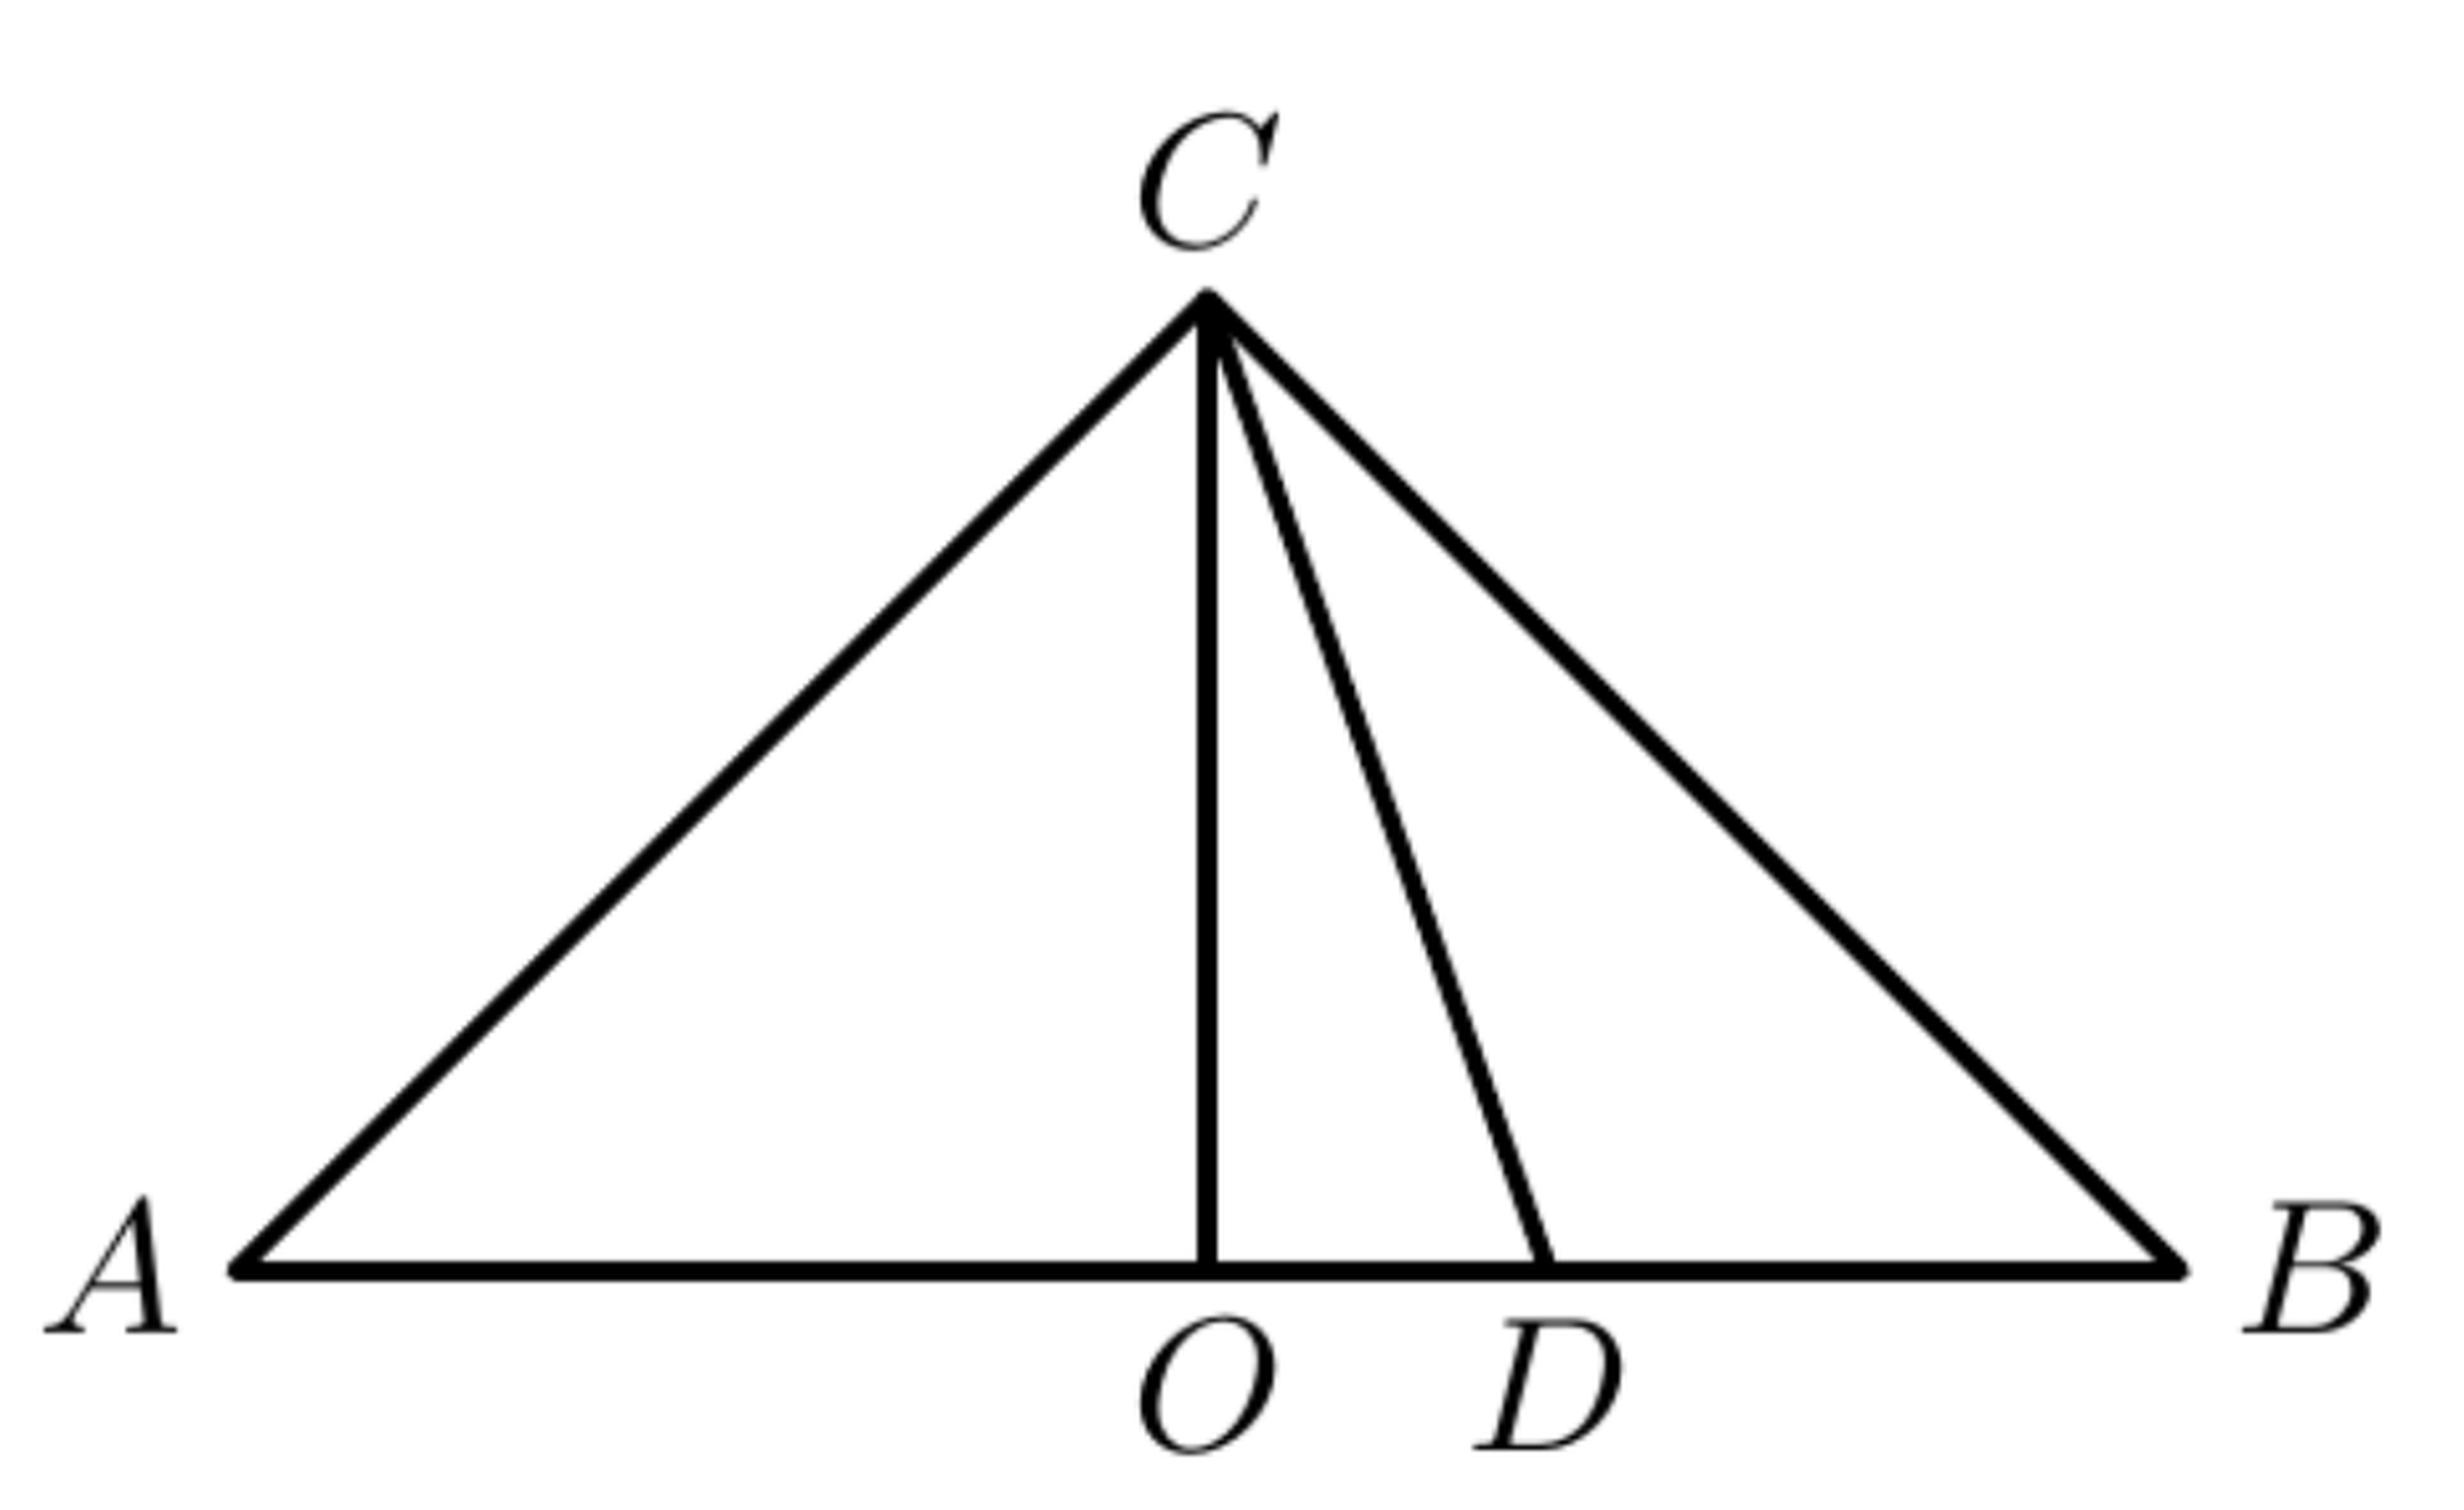
\includegraphics[width=0.34\textwidth]{figures/gao160_q16.png}
\end{center}

\keepwithprev
A. $\dfrac{a+b}{2}\geqslant\sqrt{ab}$ ($a>0,b>0$)\qquad B. $a^2+b^2\geqslant2\sqrt{ab}$ ($a>0,b>0$)

C. $\dfrac{a+b}{2}\leqslant\sqrt{\dfrac{a^2+b^2}{2}}$ ($a>0,b>0$)\qquad D. $\dfrac{2ab}{a+b}\leqslant\sqrt{ab}$ ($a>0,b>0$)

\ifanswer
\solbegin
\step{$CO=AO=\dfrac{a+b}{2},OD=\left\lvert a-\dfrac{a+b}{2}\right\rvert=\dfrac{\lvert a-b\rvert}{2}$，}
\step{$CD=\sqrt{CO^2+OD^2}=\sqrt{\dfrac{a^2+b^2}{2}}\geqslant CO=\dfrac{a+b}{2}$，}
\step{等号当且仅当 $a=b$ 时成立，故选 $C$.}
\solend
\fi

\end{enumerate}

\bigsec{三、解答题}

\begin{enumerate}
\setcounter{enumi}{16}

% === Q17 === cases 块算一行；判别式印等腰偏高三角 \Delta；解析 7 行
\item 已知幂函数 $f(x)=(m^2-2m-2)x^{m-1}$ 在 $(0,+\infty)$ 上是严格增函数.

(1) 求 $m$ 的值；

(2) 若关于 $x$ 的方程 $f(x)=(t+1)x-t^2$ 有两个不相等的正实根，求实数 $t$ 的取值范围.

\ifanswer
\solbegin
\step{(1) 幂函数的系数为 1，因此 $m^2-2m-2=1\Leftrightarrow(m-3)(m+1)=0$，}
\step{解得 $m=3$ 或 $m=-1$.}
\step{由 $f(x)$ 在 $(0,+\infty)$ 上严格递增，得 $m-1>0$，所以 $m=3$，}
\step{此时 $f(x)=x^2$.}
\step{(2) 原方程化为 $x^2-(t+1)x+t^2=0$，}
\step{方程有两个不相等的正实根，则 $\begin{cases}\Delta=(t+1)^2-4t^2=(1-t)(3t+1)>0\\t+1>0\\t^2>0\end{cases}$，}% 判别式原卷印等腰偏高三角 \Delta，照录
\step{得 $t\in\left(-\dfrac{1}{3},0\right)\cup(0,1)$.}
\solend
\fi

% === Q18 === 补集上划线 \overline{A}、\subseteq 带下划线、\varnothing；解析 8 行
\item 已知集合 $A=\{x\mid\lvert x-a\rvert<a-3\}$，$B=\left\{x\mid\dfrac{x+1}{x-2}\geqslant2\right\}$.

(1) 若 $a=5$，求 $\overline{A}\cap B$；

(2) 若 $A\cap B=A$，求实数 $a$ 的取值范围.

\ifanswer
\solbegin
\step{(1) $\dfrac{x+1}{x-2}\geqslant2\Leftrightarrow\dfrac{5-x}{x-2}\geqslant0\Leftrightarrow2<x\leqslant5,B=(2,5]$，}
\step{当 $a=5$ 时，$A=\{x\mid\lvert x-5\rvert<2\}=(3,7)$，于是 $\overline{A}=(-\infty,3]\cup[7,+\infty)$，}
\step{因此 $\overline{A}\cap B=(2,3]$.}
\step{(2) $A\cap B=A$ 等价于 $A\subseteq B$.}
\step{当 $a\leqslant3$ 时，$a-3\leqslant0$，$A=\varnothing$，满足条件.}
\step{当 $a>3$ 时，$\lvert x-a\rvert<a-3\Leftrightarrow3<x<2a-3,A=(3,2a-3)$，}
\step{此时 $A\subseteq B=(2,5]$ 等价于 $2a-3\leqslant5$，即 $a\leqslant4$，结合 $a>3$ 得 $3<a\leqslant4$.}
\step{合并两种情形，实数 $a$ 的取值范围为 $(-\infty,4]$.}
\solend
\fi

% === Q19 === 数据表 tabular 重排（高一130 成例）；cases 块算一行；解析 6 行
\item 作为我国最高水平的综合性运动会，全运会汇聚了国内顶尖体育健儿，某代表队从第 8 届全运会开始登上赛场，且参赛运动员人数逐年递增. 设 $t$ 为该代表队参赛后经过的届数，即第 8 届为 $t=0$，第 9 届为 $t=1$，以此类推. 经过 $t$ 届，运动员人数为 $y$ 人，具体数据如下：

\begin{center}
\begin{tabular}{cccccc}
$t$ & 0 & 1 & 2 & 3 & 4 \\
\hline
届数 & 8 & 9 & 10 & 11 & 12 \\
运动员人数（$y$ 人） & 4 & 11 & 25 & 53 & 109
\end{tabular}
\end{center}

(1) 现有以下两种函数模型：① $y=a\cdot b^t+c$ ($a>0,b>1$)；② $y=\log_a(t+b)+c$ ($b>0,a>1$). 请根据上表中运动员人数的增长规律，选出你认为符合的函数模型（不用说明理由），并利用表中前 3 组数据求出相应的函数解析式；

(2) 若参赛运动员人数按照 (1) 中求得的模型继续增长，在第几届全运会时，该代表队运动员人数将会首次超过 1000 人？

\ifanswer
\solbegin
\step{(1) 选模型①，将前 3 组数据代入，得 $\begin{cases}a+c=4\\ab+c=11\\ab^2+c=25\end{cases}$，}% 原卷印"选模型①"（圈数字①），OCR 误作"四"，照录①，见头注 ⑤ 3
\step{相邻两式相减，得 $a(b-1)=7$，$ab(b-1)=14$，}
\step{两式相除得 $b=2$，进而 $a=7$，$c=-3$，所求函数解析式为 $y=7\cdot2^t-3$.}
\step{(2) $y=7\cdot2^t-3$ 随 $t$ 的增大而增大，且 $t=7$ 时，$y=893<1000$；}
\step{$t=8$ 时，$y=1789>1000$，}
\step{$t$ 为非负整数，首次超过 1000 人时 $t=8$，对应第 $8+8=16$ 届全运会.}
\solend
\fi

% === Q20 === 解析 12 行（跨 08—09 页）
\item 已知函数 $f(x)=\log_a(a-a^x)$.

(1) 求该函数的定义域；

(2) 若 $a>1$，试判断关于 $x$ 的方程 $f(x)=2$ 是否有实数解，并说明理由；

(3) 若当 $x\in(-\infty,0]$ 时，关于 $x$ 的不等式 $f(x)\geqslant-1$ 恒成立，求实数 $a$ 的取值范围.

\ifanswer
\solbegin
\step{(1) 对数的底数须满足 $a>0$ 且 $a\ne1$，真数须满足 $a-a^x>0$，即 $a^x<a^1$.}% 原卷印 $a^1$，照录未化简，见头注 ⑤ 4
\step{当 $a>1$ 时，$x<1$，定义域为 $(-\infty,1)$.}
\step{当 $0<a<1$ 时，$x>1$，定义域为 $(1,+\infty)$.}
\step{(2) 当 $a>1$ 时，若 $f(x)=2$，则 $a-a^x=a^2\Rightarrow a^x=a(1-a)<0$，}
\step{这与 $a^x>0$ 矛盾，因此方程无实数解.}
\step{(3) 不等式在 $(-\infty,0]$ 上恒成立，须先保证该区间包含于函数的定义域，}
\step{由 (1) 得 $a>1$.}
\step{当 $x\leqslant0$ 时，$0<a^x\leqslant1$，所以 $a-a^x\geqslant a-1>0$.}
\step{由对数函数的单调性，$f(x)=\log_a(a-a^x)\geqslant\log_a(a-1)=f(0)$，}
\step{等号当且仅当 $x=0$ 时成立，}
\step{因此所求条件等价于 $\log_a(a-1)\geqslant-1\Leftrightarrow a-1\geqslant\dfrac{1}{a}\Leftrightarrow a^2-a-1\geqslant0$，}
\step{结合 $a>1$，得 $a\in\left[\dfrac{1+\sqrt{5}}{2},+\infty\right)$.}
\solend
\fi

% === Q21 === "和积平衡集"定义证明题；\N；解析 18 行（跨 09—10 页）
\item 已知有限集 $A=\{a_1,a_2,\cdots,a_n\}$ ($n\geqslant2,n\in\N$)，如果 $A$ 中元素 $a_i$ ($i=1,2,3,\cdots,n$) 满足 $a_1+a_2+a_3+\cdots+a_n=a_1\times a_2\times\cdots\times a_n$，就称 $A$ 为“和积平衡集”.

(1) 分别判断集合 $A=\{1,2,3,4\}$，$B=\{4+2\sqrt{2},4-2\sqrt{2}\}$ 是否为“和积平衡集”；

(2) 已知 $a_1$、$a_2$ 是两个不同的正数，且 $\{a_1,a_2\}$ 是“和积平衡集”，请用反证法证明：$a_1$、$a_2$ 至少有一个大于 2；

(3) 若 $a_i\geqslant1$，且 $a_i\in\N$，求所有符合条件的“和积平衡集”.

\ifanswer
\solbegin
\step{(1) 因为 $1+2+3+4=10\ne24=1\times2\times3\times4$，所以 $A$ 不是“和积平衡集”.}
\step{因为 $(4+2\sqrt{2})+(4-2\sqrt{2})=8=(4+2\sqrt{2})(4-2\sqrt{2})$，}
\step{所以 $B$ 是“和积平衡集”.}
\step{(2) 假设 $a_1$、$a_2$ 都不大于 2，则 $\dfrac{1}{a_1}\geqslant\dfrac{1}{2},\dfrac{1}{a_2}\geqslant\dfrac{1}{2}$，}
\step{由于 $a_1\ne a_2$，上述两个不等式至少有一个严格成立.}
\step{而 $a_1+a_2=a_1a_2$，两边除以 $a_1a_2>0$，得 $1=\dfrac{1}{a_1}+\dfrac{1}{a_2}>\dfrac{1}{2}+\dfrac{1}{2}=1$，矛盾，}
\step{所以 $a_1$、$a_2$ 至少有一个大于 2.}
\step{(3) 不妨设 $a_1<a_2<\cdots<a_n$，由各元素均为正整数，得 $a_i\geqslant i$.}
\step{若 $n\geqslant4$，因其余因子均不小于 1，}
\step{有 $a_1a_2\cdots a_n\geqslant a_2a_{n-1}a_n\geqslant2(n-1)a_n>na_n>a_1+a_2+\cdots+a_n$，}
\step{与和积平衡条件矛盾，因此只需讨论 $n=2,3$.}
\step{当 $n=2$ 时，$a_1+a_2=a_1a_2\Leftrightarrow(a_1-1)(a_2-1)=1$，}
\step{两个因子均为非负整数，只能有 $a_1=a_2=2$，与元素互不相同矛盾.}
\step{当 $n=3$ 时，若 $a_1\geqslant2$，则 $a_2\geqslant3$，从而 $a_1a_2a_3\geqslant6a_3>3a_3>a_1+a_2+a_3$，}
\step{矛盾，因此 $a_1=1$.}
\step{此时 $1+a_2+a_3=a_2a_3\Leftrightarrow(a_2-1)(a_3-1)=2$，}
\step{由 $1\leqslant a_2-1<a_3-1$，得 $a_2-1=1$、$a_3-1=2$，即 $a_2=2$、$a_3=3$.}
\step{检验 $1+2+3=1\times2\times3=6$，所求集合为 $\{1,2,3\}$.}
\solend
\fi

\end{enumerate}

\end{document}
"
% 紧凑版：xelatex "\def\iscompact{1}% 高一160_奉贤中学_期中.tex
%   —— 高一上数学"2026-2027 年奉贤中学高一上期中"（试卷版/答案版/紧凑版）
% 试卷版：xelatex 高一160_奉贤中学_期中.tex
% 答案版：xelatex "\def\isanswer{1}% 高一160_奉贤中学_期中.tex
%   —— 高一上数学"2026-2027 年奉贤中学高一上期中"（试卷版/答案版/紧凑版）
% 试卷版：xelatex 高一160_奉贤中学_期中.tex
% 答案版：xelatex "\def\isanswer{1}% 高一160_奉贤中学_期中.tex
%   —— 高一上数学"2026-2027 年奉贤中学高一上期中"（试卷版/答案版/紧凑版）
% 试卷版：xelatex 高一160_奉贤中学_期中.tex
% 答案版：xelatex "\def\isanswer{1}\input{高一160_奉贤中学_期中.tex}"
% 紧凑版：xelatex "\def\iscompact{1}\input{高一160_奉贤中学_期中.tex}"
%
% ① 原始材料：微信公众号"魔都数学加油站"文章，连载"27学年高一160"，原卷卷面标题
% "2026-2027 年奉贤中学高一上期中"（卷面未印副标题、未印连载号）。
% 正文为 10 张 PNG 页（01/04/10 为 2560×3620，02/03/05/06/07/08/09 为
% 4762×6735，同一篇各页分辨率混排，逐页按各自分辨率裁图核对）。
% 体例：讲评版——填空 3—12（10 题）、选择 13—16（4 题）、解答 17—21（5 题），
% 共 19 题，自第 3 题起编（1、2 未印在本篇）；19 题逐题印【解析】，无只印【答案】
% 的题；四道选择题答案在解析末句"故选 $B$/$B$/$D$/$C$"，题干括号
% \mbox{（\quad）} 留空、不另提 \ans{}。题目、答案、解析均据原图转录；卷面粉红色
% 水印"魔都数学加油站"及公众号页脚未录入。
% 全卷插图清单（逐页通读 10 页确认）：2 幅，均为题目配图、三版都出——
%   · Q4 韦恩图（01 页右侧：矩形全集 U、两圆 A/B、阴影部分 B∩上划线 A、
%     标注 U/A/B），裁 figures/gao160_q4.png；
%   · Q16 等腰直角三角形 ABC 图（05 页右下：C 顶点、A/O/D/B 共线底边、
%     CO 与 CD 两条线段），裁 figures/gao160_q16.png；
%   两图均取原卷截图 3—4× LANCZOS 放大、去粉色水印、转灰度、autocontrast；
%   Q4 图左侧题干残字"示"、Q16 图左侧题干残字均已裁白。
%   Q19 有一张 3 行数据表（t／届数／运动员人数（y 人），t=0..4），按全稿
%   成例（高一130）用 tabular 重排，不做成 png；其余各页无题目配图、
%   无解析内配图、无其它表格、无"如图"处。
%
% 卷首标题：原卷印作"2026-2027 年奉贤中学高一上期中"，年份区间按全稿惯例排 en dash；
% 原卷卷面未印副标题，本稿按同期中卷知识模块口径补出"集合与常用逻辑用语、不等式、函数"。
%
% ② 与原卷的排版差异／照录项清单：
%   ① 原文从第 3 题起，本稿保留原题号；共 19 题三节，解答题 5 题到 21；
%      三节各自一个 enumerate + \setcounter{enumi}{2}/{12}/{16}（不贯穿），
%      用 \examtitlest[3] 起手；
%   ② 混合体例说明：19 题全印【解析】、用 \solbegin…\solend，无只印【答案】
%      或答案印括号内的题；四道选择题答案在解析末句"故选 $B$/$B$/$D$/$C$"
%      （逐个放大复核）、括号 \mbox{（\quad）} 留空、不另提 \ans{}；答案版
%      【答案】/【解析】标记数 = 19 = 全卷题数（0 个 \ans ＋ 19 个 \solbegin）；
%   ③ 原卷卷面未印副标题，本稿按知识模块口径补出；
%   ④ 原卷填空横线按全稿惯例排 \blankline[4.4em]；选择题括号排 \mbox{（\quad）}、
%      四道选择题的选项段前按惯例各加 \keepwithprev；解答题不留作答区、不加
%      \anspace（原卷为讲评版，109—113 起全稿不用 \anspace）；
%   ⑤ 数集归一：Q4"$U=\Z$"、Q9"$a\in\R$，$b\in\R$"、Q11"$n\in\Z$"、
%      Q15"$s\in\R$"、Q21"$n\in\N$""$a_i\in\N$"原卷印正体粗体 Z/R/N，
%      按全稿惯例归一 \Z／\R／\N；集合描述竖线排 \mid（Q3、Q4、Q12、
%      Q18、Q21）；空集 \varnothing（Q18 解析 (2)）；补集照原卷上划线排
%      \overline{A}（Q4 解析、Q18 (1) 题干与解析）；子集符号 Q18 两处
%      "$A\subseteq B$"印带下划线 ⊆、照录 \subseteq；
%   ⑥ 绝对值排 \lvert…\rvert（Q7、Q8 题干与解析、Q9 题干、Q16 解析、
%      Q18 题干与解析），Q16 解析的 \left\lvert…\right\rvert 与 \lvert…\rvert
%      均在同一 $…$ 组内配对平衡；
%   ⑦ 判别式两形混用逐处照录不统一（放大逐处确认）：Q3 解析
%      "$\triangle=1^2-4a\times\frac{1}{4}=0$"原卷印扁等边三角、照录
%      \triangle；Q17 解析 cases 块"$\Delta=(t+1)^2-4t^2=(1-t)(3t+1)>0$"
%      原卷印等腰偏高三角、照录 \Delta；Q16 题干几何符号"$\triangle ABC$"
%      按全稿几何三角形记号惯例归一 \triangle（参照 高一150／132 成例）；
%   ⑧ 不等号按全稿惯例排 \leqslant／\geqslant；中文弯引号照录：Q9 题干
%      "充分非必要""必要非充分""充要""既非充分又非必要"、Q14 题干
%      "存在 $x\in(1,+\infty)$，使得 $f(x)>0$"与解析"存在""对任意"、
%      Q21 题干与解析多处"和积平衡集"；注释里一律 ASCII 引号；
%   ⑨ 文本圈数字逐处照录：Q12 题干①②③、Q12 解析"故①正确""同②得"
%      "故②正确""③假设""故③错误""故真命题是①②"、Q19 题干①②与解析
%      "选模型①"，均为印刷圈数字（非 \textcircled、非数学模式）；
%   ⑩ 半角逗号在数学组之间是全稿惯例、非笔误，逐处照录（Q8"$2^t,2^{-t}$"、
%      Q9"$a=-1,b=-2$""$a=1,b=-1$"、Q11"$1\leqslant a<10,n\in\Z$"、
%      Q12"$s_1=\frac{1}{2},t_1=x_n$"、Q16 选项"$a>0,b>0$"与解析
%      "$CO=AO=\frac{a+b}{2},OD=...$"、Q18"$2<x\leqslant5,B=(2,5]$"
%      "$3<x<2a-3,A=(3,2a-3)$"、Q21"$n=2,3$"等）；行中全角逗号／顿号
%      照录（Q15 选项"$a>1$，且 $s>0$"、Q12 解析"$s$、$t$"、Q21 解析
%      "$a_1$、$a_2$"），顿号一律移出数学模式；
%   ⑪ "图像／图象"逐处照录：本卷 Q5"的图像恒过一个定点"、Q10"的图像经过点"、
%      Q13 题干两处"图像"与解析"对称图像对应的函数"均印"图像"（有亻）；
%      Q16 印"图形"（利用图形说明、该图形能说明），无"图象"用例；
%   ⑫ 复杂式照录别简化：Q3 $ax^2+x+\frac14=0$、Q5 $y=\log_a(5x-9)-4$、
%      Q6 $(1-2x)^{\frac34}>x^{\frac34}$ 与 $\left[0,\frac12\right]$、
%      Q8 $\frac{s+\sqrt{s^2-4}}{2}$、Q10 $y=\frac{2^x}{2^x+ax}$ 与
%      $\frac{2^p}{2^p+ap}=\frac56$、$\frac{2^q}{2^q+aq}=\frac16$、
%      Q11 $N=a\times10^n$ 与 $3^{2026}$、$2026\lg3\approx966.60$、
%      $966.64512<2026\lg3<966.66538$、Q12 $Y=\{(s,t)\mid s\in X,t\in X\}$
%      与 $\frac12 s+tx_n=0$、Q16 $\sqrt{\frac{a^2+b^2}{2}}$、
%      Q17 $x^2-(t+1)x+t^2=0$ 与 $\left(-\frac13,0\right)\cup(0,1)$、
%      Q18 $\frac{5-x}{x-2}\geqslant0$、Q19 $y=a\cdot b^t+c$ 与
%      $y=\log_a(t+b)+c$、$y=7\cdot2^t-3$、Q20 $f(x)=\log_a(a-a^x)$
%      与 $a^2-a-1\geqslant0$、$\left[\frac{1+\sqrt5}{2},+\infty\right)$、
%      Q21 $4+2\sqrt2$ 与 $(a_2-1)(a_3-1)=2$ 等；
%   ⑬ 子题标号 (1)(2)(3) 按全稿惯例排半角括号；行末／行中句点按全稿惯例
%      排 ASCII `.`（不是全角「．」）；cases 块整体算一个印刷行
%      （Q17 解析、Q19 解析 (1)）；
%   ⑭ 配图：Q4／Q16 题目配图（三版都出）放 \item 内题干之后 \begin{center}，
%      各用 \needvspace{8cm} 守卫把整块推走，**守卫放在 \item 之前**
%      （见 高一153 Q11/Q19 成例与切页审计 B 类坑）；
%   ⑮ 一条 \step = 原卷解析的一个印刷行；跨上下半页的重叠行只算一次
%      （Q4 解析、Q9 解析首行、Q11 解析首行、Q12 解析"若 $s=-1$…"一行、
%      Q18 解析"此时 $A\subseteq B=(2,5]$…"一行、Q20 (2) 题干、
%      Q21 解析"由 $1\leqslant a_2-1<a_3-1$…"一行）；原卷折行别合并；
%   ⑯ Q10 之后另有一整块【注】按语（03 页上半，5 个印刷行），是讲评版作者对
%      原卷数据自相矛盾的加注、不属于任何题的【解析】。本稿按 高一53
%      "注：…"成例放 Q10 的 \solend 之后、Q10 的 \fi 收尾之前：
%      **整块只保留 Q10 那一层外层 \ifanswer**（那个 \fi 就是 Q10 的收尾），
%      块内 \stepm{【注】}{首行} ＋ 4 条 \step 各自自带内层 \ifanswer…\fi
%      （\step／\stepm 宏内自带，源码里不手动再包一层 \ifanswer，
%      否则 题目溯源.py 的 strip_answers 非贪婪正则会错切）；
%      \stepm 第一参数直接用「【注】」作标签，与全稿 \ans 的【答案】、
%      \solbegin 的【解析】同性质，未加粗以外不另加任何样式；
%      5 行仅答案版出、不新增 \item、不影响溯源，头注 ③ 单列登记、
%      不计入 19 题逐题 \step 账；\stepm 把【注】排成加粗着色标签
%      （原卷为黑色加粗），此一处着色差异在此登记；
%   ⑰ 原卷用字照录：Q11"约翰·纳皮尔""莱布尼兹"（原卷作"兹"，非通行"茨"）、
%      "17 世纪的三大数学发明"；Q16"数学说明的方法""点 $D$ 为斜边 $AB$ 上
%      异于顶点的一个动点"；Q19"登上赛场""以此类推"；
%
% ③ 行数复核：一条 \step = 原卷解析的一个印刷行，cases 块作一个印刷行计。
%   逐题数（逐页核对定稿）：Q3：5；Q4：1；Q5：1；Q6：2；Q7：2；Q8：4；
%   Q9：4；Q10：3；Q11：6；Q12：19；Q13：1；Q14：2；Q15：3；Q16：3；
%   Q17：7；Q18：8；Q19：6；Q20：12；Q21：18。
%   合计 107 条 \step（19 题逐题印刷行账），与原卷逐题印刷行相等。
%   **本卷源码 \step 总数 = 19 题逐题合计 107 ＋ Q10 后独立【注】块 5 行
%   = 112 行**（其中 \step 111 条、\stepm 1 条；\stepm 与 4 条 \step 合为
%   【注】块 5 印刷行）。该 5 行不计入「逐题印刷行」账，也不是任何题的
%   【解析】，而是讲评版编者按语；主会话核验脚本按全文统计 \step 时总数会
%   较逐题账多 5，已与主会话对齐、属已知预期而非错误。
%   全卷 19 题均设 \solbegin…\solend，答案版【答案】/【解析】标记数
%   = 19 = 全卷题数。
%
% ④ 页码分布（供回原图复核）：
%   卷首标题＋"一、填空题"＋Q3 题干＋解析 5 行＋Q4 题干＋韦恩图＋解析
%   1 行＋Q5 题干首行在 01 页上半；Q4 解析（重叠）＋Q5 题干续＋解析 1 行＋
%   Q6 题干＋解析 2 行＋Q7 题干＋解析首行在 01 页下半；Q7 解析末行＋
%   Q8 题干＋解析 4 行＋Q9 题干＋解析首行在 02 页上半；Q9 解析（重叠首行）
%   ＋余 3 行＋Q10 题干＋解析 3 行在 02 页下半；【注】按语 5 行＋Q11 题干＋
%   解析首行在 03 页上半；Q11 解析（重叠首行）＋余 5 行＋Q12 题干＋①②
%   在 03 页下半；Q12 ③＋解析前 9 行在 04 页上半；Q12 解析（重叠 2 行）
%   ＋余 8 行在 04 页下半；Q12 解析末 2 行＋"二、选择题"＋Q13 题干＋选项＋
%   解析 1 行＋Q14 题干＋选项＋解析首行在 05 页上半；Q14 解析末行＋
%   Q15 题干＋选项＋解析 3 行＋Q16 题干＋三角形图在 05 页下半；
%   Q16 选项＋解析 3 行＋"三、解答题"＋Q17 题干＋两问在 06 页上半；
%   Q17 解析 7 行在 06 页下半；Q18 题干＋两问＋解析前 7 行＋Q19 题干首行
%   在 07 页上半；Q18 解析末行（重叠）＋Q19 题干＋表格＋两问在 07 页下半；
%   Q19 解析 6 行＋Q20 题干＋(1)(2) 在 08 页上半；Q20 (2)(3) 题干（重叠）
%   ＋解析 8 行在 08 页下半；Q20 解析末 4 行＋Q21 题干＋(1)(2) 在 09 页
%   上半；Q21 (3)＋解析前 7 行在 09 页下半；Q21 解析 (3) 余 10 行在 10 页
%   上半；Q21 末行（重叠）＋"检验 $1+2+3=1\times2\times3=6$，所求集合为
%   $\{1,2,3\}$."在 10 页下半（此后仅水印、无正文）。本稿按题连排，
%   不丢行、不并折行；全卷末题为第 21 题，无附加题节。
%
% ⑤ 存疑照录（放大原图确认，照录未改、正文对应处另有 % 注）：
%   1. Q10【注】按语：讲评版作者据 $a=\sqrt3$ 时 $2^q=\frac{\sqrt3}{5}q<q$
%      与 $2^n\geqslant n+1$ 推出点 $Q$ 不存在、"严格说本题无解"，并注明
%      "原卷数据疑似有误（同型常见题为 $P(p,\frac65)$、$Q(q,-\frac15)$、
%      $2^{p+q}=36pq$，得 $a=6$）"；本稿照录全块、未删未改（见 ② ⑯）。
%   2. Q12 解析 (3) 末段"若 $t=-1$，则 $\frac{1}{2}s=x_n\cdot(-1)$，
%      于是 $s=2x_n>x_n$，也矛盾，"中，等式右端与紧随的结论符号不自洽
%      （按题意应为 $\frac12 s=x_n$ 或 $-\frac12 s=x_n\cdot(-1)$），逐页
%      放大 04 页确认原卷即如此印、无漏看的负号，照录未改，建议主会话
%      回 04 页再放大复核一次；
%   3. Q19 解析 (1) 印"选模型①"（圈数字①，题干只有①②两种模型）；
%      OCR 误作"选模型四"，放大 08 页确认是①、照录①；
%   4. Q20 解析 (1)"即 $a^x<a^1$"末项原卷印 $a^1$（非 $a$），照录未化简；
%   5. Q11 题干"莱布尼兹"原卷作"兹"（非通行"茨"）、"约翰·纳皮尔"用
%      间隔号·，均照录未改；
%   6. Q9 题干"则 $p$ 是 $q$___条件"与解析"故 $p$ 是 $q$ 的充分非必要条件"
%      句式略异，均照录；
%   7. Q19 解析 (1) 用"前 3 组数据"、题干表格列到 $t=4$，照录未补。
%
\documentclass[a4paper,11pt]{article}
\usepackage{common}

\begin{document}

\examtitlest[3]{2026--2027 年奉贤中学高一上期中}{集合与常用逻辑用语、不等式、函数}

\bigsec{一、填空题}

\begin{enumerate}
\setcounter{enumi}{2}

% === Q3 === 解析 5 行；判别式印扁等边三角 \triangle
\item 若集合 $A=\{x\mid ax^2+x+\dfrac{1}{4}=0\}$ 有且仅有两个子集，则实数 $a=$\blankline[4.4em].

\ifanswer
\solbegin
\step{若集合 $A=\{x\mid ax^2+x+\dfrac{1}{4}=0\}$ 有且仅有两个子集，}
\step{所以方程 $ax^2+x+\dfrac{1}{4}=0$ 只有一个实数根，}
\step{当 $a=0$ 时，方程化为 $x+\dfrac{1}{4}=0$，解得 $x=-\dfrac{1}{4}$，符合题意，}
\step{当 $a\ne0$ 时，则 $\triangle=1^2-4a\times\dfrac{1}{4}=0$，解得 $a=1$，}% 判别式原卷印扁等边三角 \triangle，照录
\step{综上所述，实数 $a=0$ 或 1.}
\solend
\fi

% === Q4 === 题目配图（三版都出）；\needvspace 守卫放 \item 之前；补集上划线 \overline{A}；解析 1 行
\needvspace{8cm}
\item 设全集 $U=\Z$，集合 $A=\{x\mid -3<x<1\}$，$B=\{-1,0,1,2\}$，用列举法表示图中阴影部分为\blankline[4.4em].

\begin{center}
% Q4 韦恩图（全集 U、A/B 两圆、阴影 B∩上划线 A）取 01 页右侧，去粉色水印、去色、4× LANCZOS 放大；三版都出
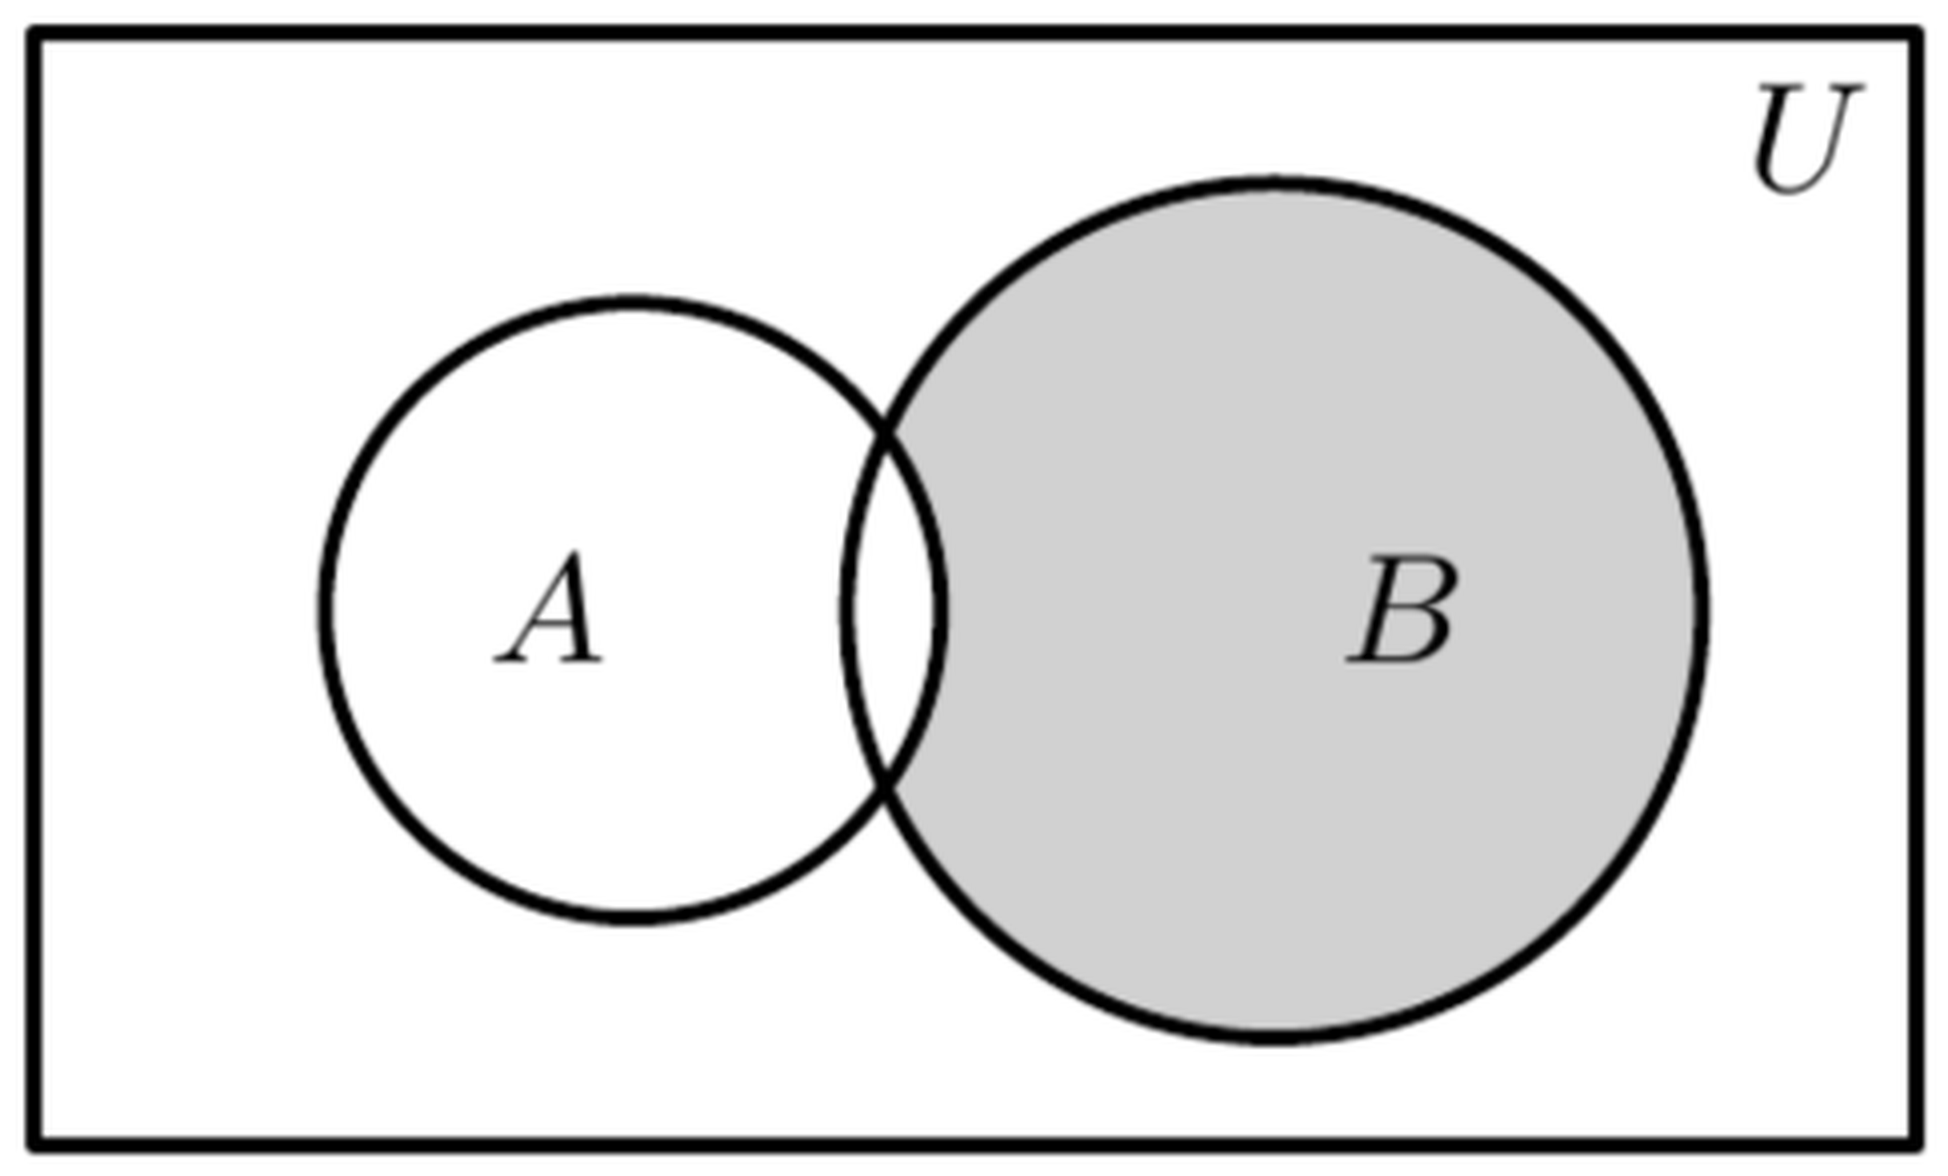
\includegraphics[width=0.38\textwidth]{figures/gao160_q4.png}
\end{center}

\ifanswer
\solbegin
\step{阴影部分表示 $B\cap\overline{A}=\{1,2\}$.}
\solend
\fi

% === Q5 === "图像"（有亻）照录；解析 1 行
\item 已知常数 $a>0$ 且 $a\ne1$，假设无论 $a$ 取何值，函数 $y=\log_a(5x-9)-4$ 的图像恒过一个定点，则这个定点的坐标为\blankline[4.4em].

\ifanswer
\solbegin
\step{$5x-9=1\Rightarrow x=2$，此时 $y=\log_a 1-4=-4$，定点为 $(2,-4)$.}
\solend
\fi

% === Q6 === 解析 2 行
\item 不等式 $(1-2x)^{\frac{3}{4}}>x^{\frac{3}{4}}$ 的解集为\blankline[4.4em].

\ifanswer
\solbegin
\step{定义域为 $\left[0,\dfrac{1}{2}\right]$，由幂函数的单调性，原不等式等价于 $1-2x>x$，}
\step{得 $0\leqslant x<\dfrac{1}{3}$，故解集为 $\left[0,\dfrac{1}{3}\right)$.}
\solend
\fi

% === Q7 === 绝对值 \lvert…\rvert；解析 2 行（跨 01—02 页）
\item 已知不等式 $\lvert x+3\rvert+\lvert x-2\rvert\geqslant 5$，当其等号成立时，$x$ 的取值范围是\blankline[4.4em].

\ifanswer
\solbegin
\step{$\lvert x+3\rvert+\lvert x-2\rvert=\lvert x+3\rvert+\lvert 2-x\rvert\geqslant\lvert(x+3)+(2-x)\rvert=5$，}
\step{等号成立当且仅当 $(x+3)(2-x)\geqslant0$，即 $x\in[-3,2]$.}
\solend
\fi

% === Q8 === 解析 4 行
\item 已知函数 $f(x)=\lvert\log_2 x\rvert$，若方程 $f(x)-t=0$ 有两个不同的实数根 $x_1,x_2$，则 $x_1+x_2$ 的取值范围是\blankline[4.4em].

\ifanswer
\solbegin
\step{方程有两个不同实根，必有 $t>0$，两根为 $2^t,2^{-t}$，}
\step{所以 $x_1+x_2=2^t+2^{-t}>2$（等号仅在 $t=0$ 时成立）.}
\step{任取 $s>2$，令 $a=\dfrac{s+\sqrt{s^2-4}}{2}>1$，取 $t=\log_2 a>0$，则 $x_1+x_2=a+\dfrac{1}{a}=s$，}
\step{所以取值范围为 $(2,+\infty)$.}
\solend
\fi

% === Q9 === 中文弯引号、\R、绝对值 \lvert…\rvert；解析 4 行
\item 已知 $a\in\R$，$b\in\R$，$p:\dfrac{1}{\lvert a\rvert}>\dfrac{1}{\lvert b\rvert}$，$q:\dfrac{1}{a}>\dfrac{1}{b}$，则 $p$ 是 $q$\blankline[4.4em]条件（用“充分非必要”、“必要非充分”、“充要”或“既非充分又非必要”填空）.

\ifanswer
\solbegin
\step{由 $p$、$q$ 中的分式有意义，$a\ne0$ 且 $b\ne0$.}
\step{当 $a=-1,b=-2$ 时，$p$ 成立而 $q$ 不成立，故 $p$ 不是 $q$ 的充分条件.}
\step{当 $a=1,b=-1$ 时，$q$ 成立而 $p$ 不成立，故 $p$ 不是 $q$ 的必要条件.}
\step{故 $p$ 是 $q$ 的充分非必要条件.}
\solend
\fi

% === Q10 === 解析 3 行；其后独立【注】按语 5 行（见头注 ② ⑯、⑤ 1）
\item 已知常数 $a>0$，函数 $y=\dfrac{2^x}{2^x+ax}$ 的图像经过点 $P\left(p,\dfrac{5}{6}\right)$、$Q\left(q,\dfrac{1}{6}\right)$，若 $2^{p+q}=3pq$，则 $a=$\blankline[4.4em].

\ifanswer
\solbegin
\step{由 $\dfrac{2^p}{2^p+ap}=\dfrac{5}{6}$ 得 $2^p=5ap$；由 $\dfrac{2^q}{2^q+aq}=\dfrac{1}{6}$ 得 $2^q=\dfrac{aq}{5}$.}
\step{$2^p>0$，$2^q>0$，$a>0$，得 $p>0$，$q>0$.}
\step{两式相乘得 $2^{p+q}=a^2pq$，又 $2^{p+q}=3pq$ 且 $pq\ne0$，故 $a^2=3$，$a=\sqrt{3}$.}
\solend
% 【注】按语（讲评版编者按，5 个印刷行，仅答案版出，不属于任何题的【解析】）
\stepm{【注】}{按原卷数据严格推敲，点 $Q$ 其实不存在：$a=\sqrt{3}$ 时 $2^q=\dfrac{\sqrt{3}}{5}q<q$；而当 $q>0$}
\step{时，取非负整数 $n$ 使 $n\leqslant q<n+1$，由 $2^{k+1}=2^k+2^k\geqslant2^k+1$ 逐次推得 $2^n\geqslant n+1$，于是}
\step{$2^q\geqslant2^n\geqslant n+1>q$，矛盾. 所以题设条件互相矛盾，严格说本题无解；$\sqrt{3}$ 是由题给关}
\step{系直接推出的值，按命题意图作为答案. 原卷数据疑似有误（同型常见题为 $P\left(p,\dfrac{6}{5}\right)$、}
\step{$Q\left(q,-\dfrac{1}{5}\right)$、$2^{p+q}=36pq$，得 $a=6$）.}% 见头注 ⑤ 1，照录未改
\fi

% === Q11 === 纳皮尔对数材料题；\Z、大数；解析 6 行
\item 17 世纪初，约翰·纳皮尔为了简化计算而发明了对数. 对数的发明是数学史上的重大事件，恩格斯曾经把笛卡尔的坐标系、纳皮尔的对数、牛顿和莱布尼兹的微积分共同称为 17 世纪的三大数学发明. 我们知道，任何一个正实数 $N$ 可以表示成 $N=a\times10^n$ ($1\leqslant a<10,n\in\Z$) 的形式，这便是科学记数法，若两边取常用对数，有 $\lg N=n+\lg a$，则可以估计 $3^{2026}$ 的最高位上的数值为\blankline[4.4em].

\ifanswer
\solbegin
\step{设 $3^{2026}=a\times10^n$ ($1\leqslant a<10,n\in\Z$)，则 $2026\lg 3=n+\lg a$.}
\step{用 $\lg 3\approx 0.4771$ 粗估，得 $2026\lg 3\approx 966.60$.}
\step{为核验误差，用 $0.47712<\lg 3<0.47713$，}
\step{得 $966.64512<2026\lg 3<966.66538$，因此 $n=966$.}
\step{于是 $\lg 4\approx 0.60206<0.64512<\lg a<0.66538<\lg 5\approx 0.69897$，}
\step{所以 $4<a<5$，最高位为 4，估算误差不影响结论.}
\solend
\fi

% === Q12 === 自定义"性质 P"；文本圈数字①②③；解析 19 行（跨 03—05 页）
\item 对于数集 $X=\{-1,x_1,x_2,x_3,\cdots,x_n\}$，其中 $0<x_1<x_2<x_3<\cdots<x_n$，$n\geqslant2$，定义点集 $Y=\{(s,t)\mid s\in X,t\in X\}$，若对于任意 $(s_1,t_1)\in Y$，存在 $(s_2,t_2)\in Y$，使得 $s_1s_2+t_1t_2=0$，则称集合 $X$ 具有性质 $P$. 则下列命题中为真命题的是\blankline[4.4em].

① $X=\{-1,1,2\}$ 具有性质 $P$；②若集合 $X$ 具有性质 $P$，则 $1\in X$；

③集合 $X$ 具有性质 $P$，若 $x_1=\dfrac{1}{2}$，则 $x_n=2$.

\ifanswer
\solbegin
\step{因为 $X=\{-1,1,2\}$，}
\step{所以 $Y=\{(-1,-1),(1,1),(2,2),(-1,1),(-1,2),(1,-1),(1,2),(2,-1),(2,1)\}$，}
\step{由集合 $X$ 具有性质 $P$ 的定义，对于任意 $(s,t)\in Y$，}
\step{若 $s>0$，$t>0$，则 $s=t$ 或 $(s,t)=(1,2)$ 或 $(s,t)=(2,1)$，}
\step{若 $s=t$，取 $s_2=-1$，$t_2=-1$，则 $ss_2+tt_2=0$；}
\step{若 $(s,t)=(1,2)$，取 $s_2=2$，$t_2=-1$，则 $ss_2+tt_2=0$；}
\step{若 $(s,t)=(2,1)$，取 $s_2=-1$，$t_2=2$，则 $ss_2+tt_2=0$；}
\step{若 $s$、$t$ 有一个为负数，则 $s=-1$ 或 $t=-1$，}
\step{若 $s=-1$，则取 $s_2=t$，$t_2=1$，则 $ss_2+tt_2=0$；}
\step{若 $t=-1$，则取 $s_2=1$，$t_2=s$，则 $ss_2+tt_2=0$；故①正确；}
\step{对于任意 $(s_1,t_1)\in Y$，存在 $(s_2,t_2)\in Y$，使得 $s_1s_2+t_1t_2=0$，}
\step{取 $(x_1,x_1)\in Y$，存在 $(x_p,x_q)$ 使得 $x_1x_p+x_1x_q=0$，所以 $x_p+x_q=0$，}
\step{不妨设 $x_p=1$，$x_q=-1$，所以若集合 $X$ 具有性质 $P$，则 $1\in X$，故②正确；}
\step{③假设 $x_n>1$，令 $s_1=\dfrac{1}{2},t_1=x_n$，则存在 $s$、$t\in X$ 使得 $\dfrac{1}{2}s+tx_n=0$，}
\step{同②得 $s$、$t$ 中必有一个数为 $-1$，}
\step{若 $s=-1$，则 $tx_n=\dfrac{1}{2}$，于是 $t=\dfrac{1}{2x_n}<\dfrac{1}{2}=x_1$，矛盾，}
\step{若 $t=-1$，则 $\dfrac{1}{2}s=x_n\cdot(-1)$，于是 $s=2x_n>x_n$，也矛盾，}% 原卷如此（与结论符号不自洽），照录未改，见头注 ⑤ 2
\step{所以 $x_n\leqslant1$，又由②得 $1\in X$，所以 $x_n\geqslant1$，所以 $x_n=1$，故③错误，}
\step{故真命题是①②.}
\solend
\fi

\end{enumerate}

% 答案版里填空解析把页排满，节标题会落到页末、与第 13 题分家（切页审计 B 类）；
% 守卫放 \bigsec 之前，连节标题一起量页高（高一157 成例）
\needvspace{7cm}
\bigsec{二、选择题}

\begin{enumerate}
\setcounter{enumi}{12}

% === Q13 === "图像"照录；解析 1 行，故选 $B$
\item 下列函数中，图像与函数 $y=3^x$ 图像关于 $y$ 轴对称的是\mbox{（\quad）}

\keepwithprev
A. $y=x^3$\qquad B. $y=\left(\dfrac{1}{3}\right)^x$\qquad C. $y=-3^x$\qquad D. $y=\log_3 x$

\ifanswer
\solbegin
\step{将 $x$ 换为 $-x$，得对称图像对应的函数为 $y=3^{-x}=\left(\dfrac{1}{3}\right)^x$，故选 $B$.}
\solend
\fi

% === Q14 === 中文弯引号；解析 2 行（跨 05 页上下），故选 $B$
\item 命题“存在 $x\in(1,+\infty)$，使得 $f(x)>0$”的否定形式为\mbox{（\quad）}

\keepwithprev
A. 不存在 $x\in(-\infty,1]$，使得 $f(x)>0$\qquad B. 对任意 $x\in(1,+\infty)$，有 $f(x)\leqslant0$

C. 对任意 $x\in(-\infty,1]$，有 $f(x)\leqslant0$\qquad D. 存在 $x\in(1,+\infty)$，使得 $f(x)\leqslant0$

\ifanswer
\solbegin
\step{将“存在”改为“对任意”，$x$ 的范围不变，并将 $f(x)>0$ 否定为 $f(x)\leqslant0$，}
\step{故选 $B$.}
\solend
\fi

% === Q15 === \R；四选项两行；解析 3 行，故选 $D$
\item 设 $a>0$，$s\in\R$. 下列各项中，能推出 $a^s>a$ 的一项是\mbox{（\quad）}

\keepwithprev
A. $a>1$，且 $s>0$\qquad B. $a>1$，且 $s<0$

C. $0<a<1$，且 $s>0$\qquad D. $0<a<1$，且 $s<0$

\ifanswer
\solbegin
\step{当 $a>1$ 时，$a^s>a\Leftrightarrow s>1$，A、B 均不能保证.}
\step{当 $0<a<1$ 时，$a^s>a\Leftrightarrow s<1$，C 不能保证，D 中 $s<0<1$，满足要求；}
\step{故选 $D$.}
\solend
\fi

% === Q16 === 题目配图（三版都出）；几何符号 \triangle ABC；解析 3 行，故选 $C$
\needvspace{8cm}
\item 数学说明的方法多种多样，其中利用图形说明就是一种重要方法. 如图所示，在等腰直角三角形 $\triangle ABC$ 中，点 $O$ 为斜边 $AB$ 的中点，点 $D$ 为斜边 $AB$ 上异于顶点的一个动点，设 $AD=a$，$BD=b$，则可用该图形能说明的不等式为\mbox{（\quad）}

\begin{center}
% Q16 等腰直角三角形 ABC 图（C/A/O/D/B 标注）取 05 页右下，去粉色水印、去色、3× LANCZOS 放大；三版都出
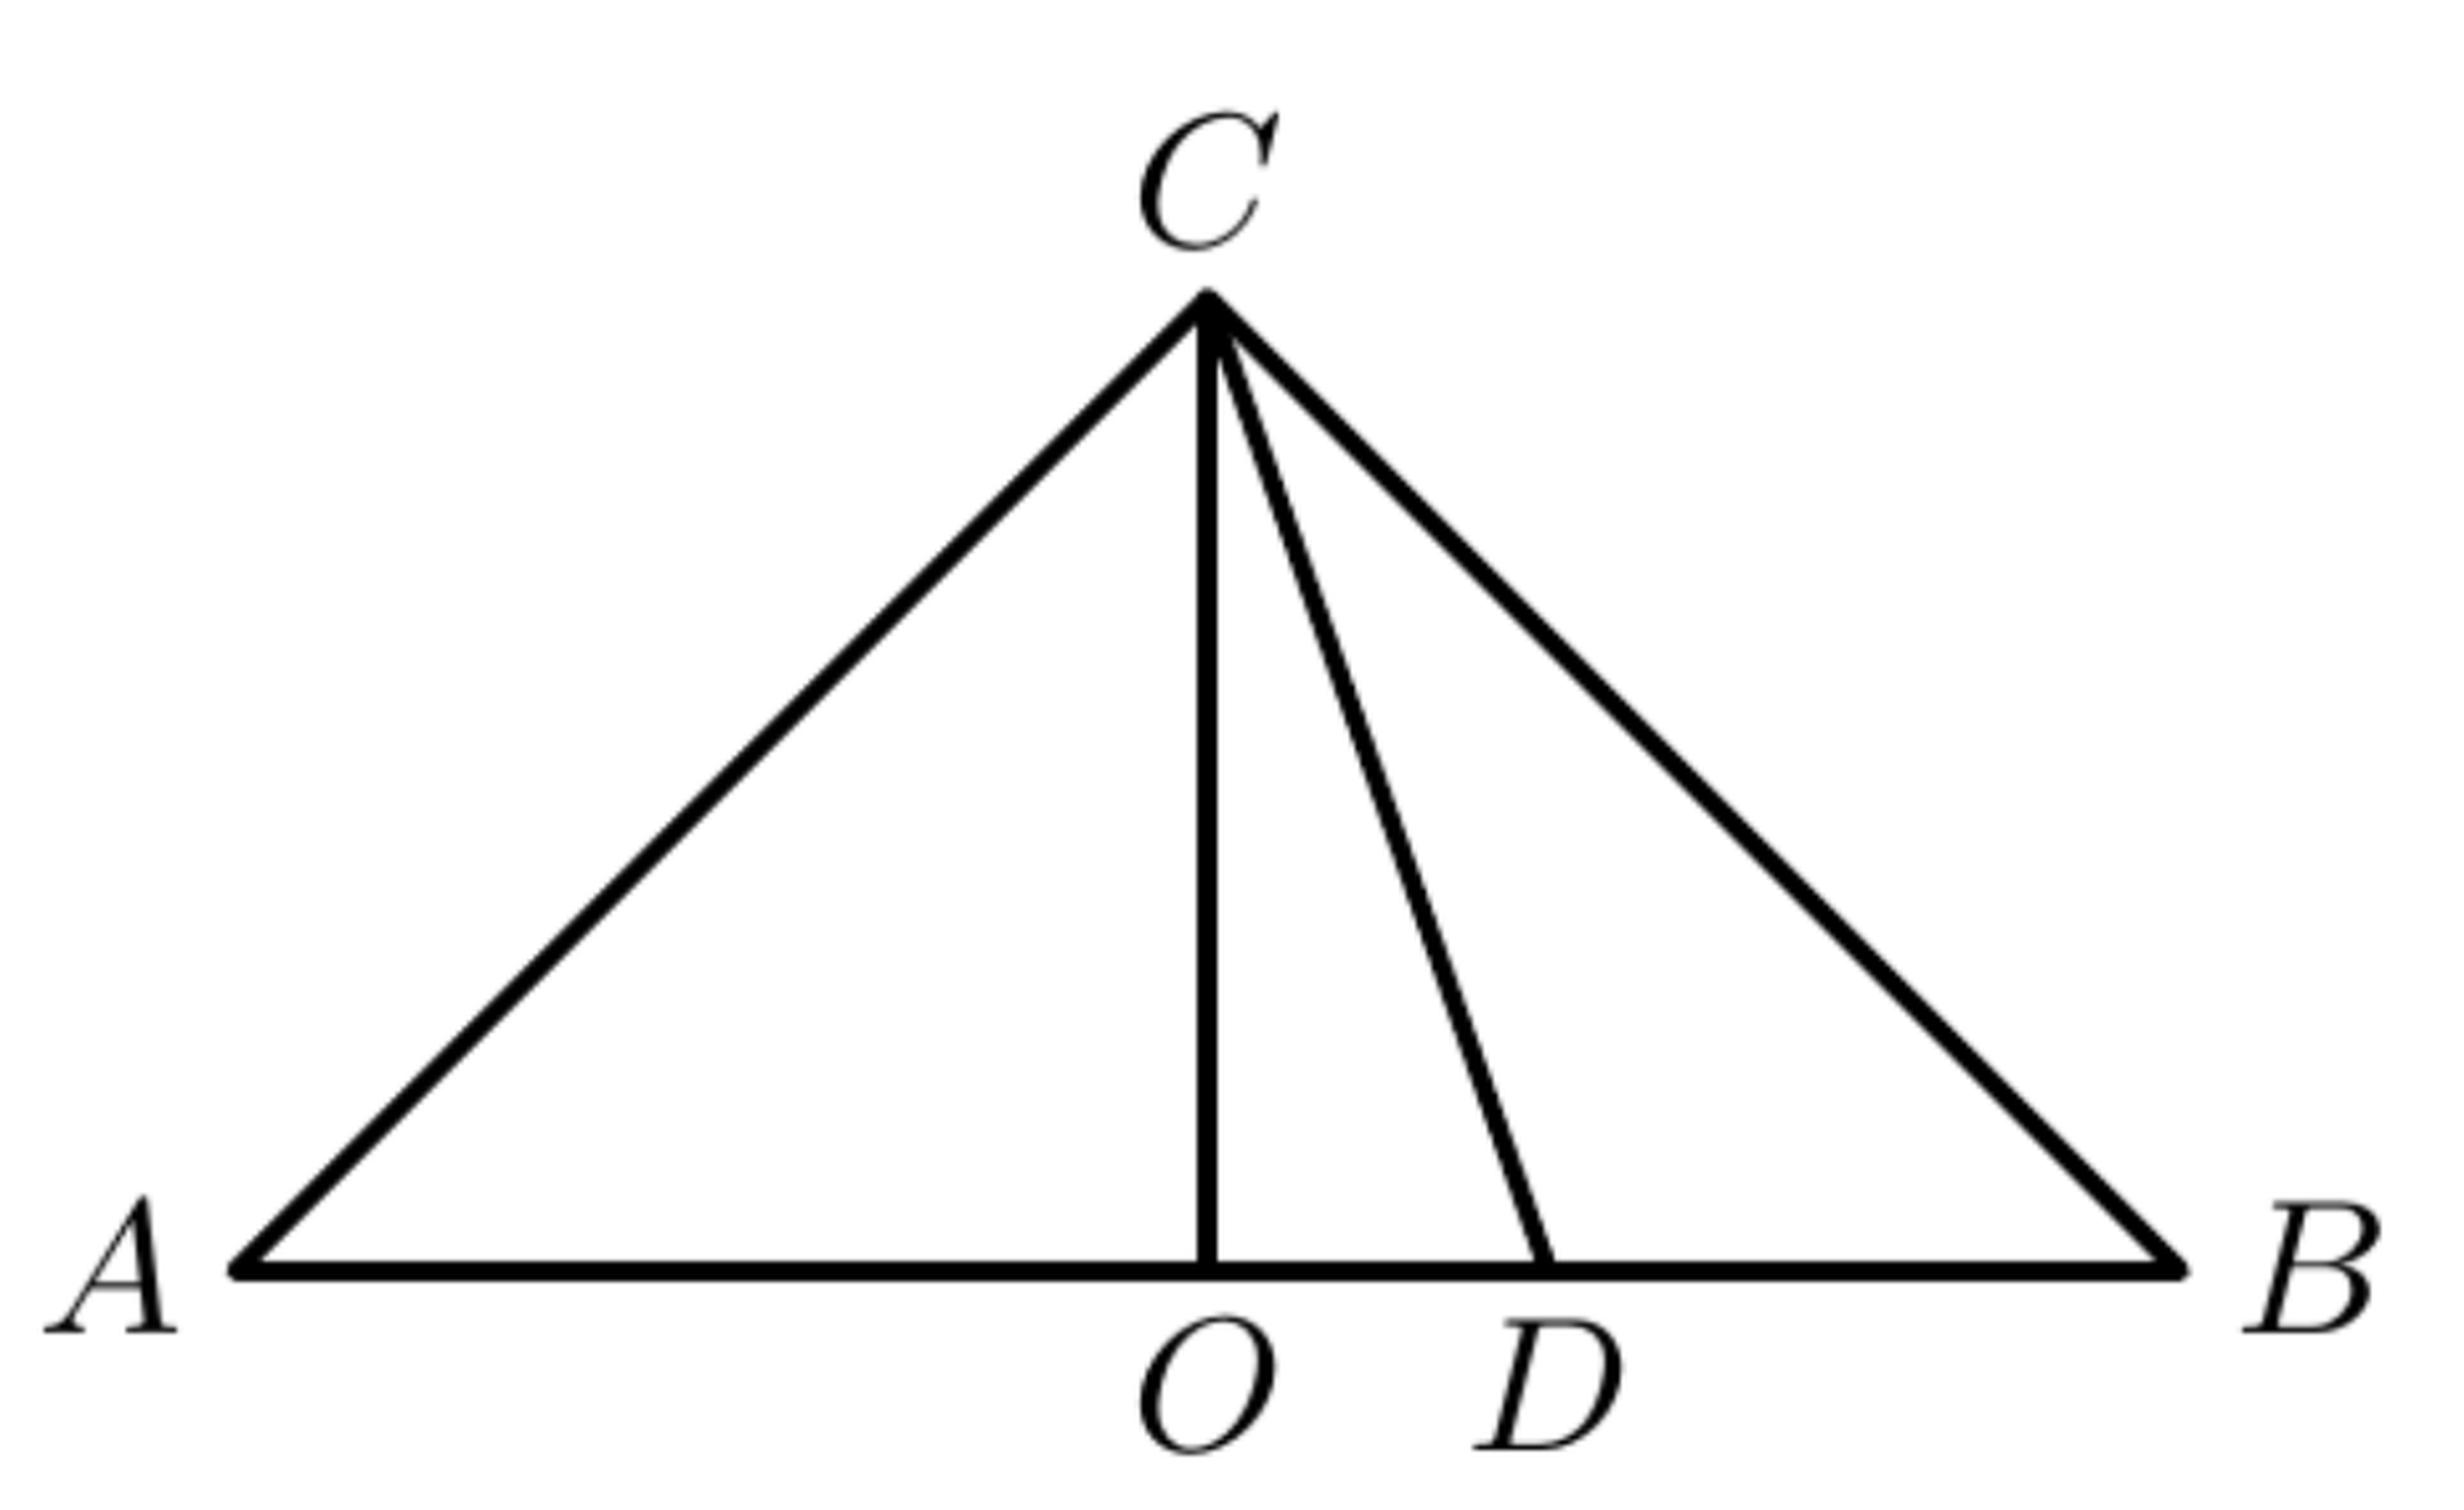
\includegraphics[width=0.34\textwidth]{figures/gao160_q16.png}
\end{center}

\keepwithprev
A. $\dfrac{a+b}{2}\geqslant\sqrt{ab}$ ($a>0,b>0$)\qquad B. $a^2+b^2\geqslant2\sqrt{ab}$ ($a>0,b>0$)

C. $\dfrac{a+b}{2}\leqslant\sqrt{\dfrac{a^2+b^2}{2}}$ ($a>0,b>0$)\qquad D. $\dfrac{2ab}{a+b}\leqslant\sqrt{ab}$ ($a>0,b>0$)

\ifanswer
\solbegin
\step{$CO=AO=\dfrac{a+b}{2},OD=\left\lvert a-\dfrac{a+b}{2}\right\rvert=\dfrac{\lvert a-b\rvert}{2}$，}
\step{$CD=\sqrt{CO^2+OD^2}=\sqrt{\dfrac{a^2+b^2}{2}}\geqslant CO=\dfrac{a+b}{2}$，}
\step{等号当且仅当 $a=b$ 时成立，故选 $C$.}
\solend
\fi

\end{enumerate}

\bigsec{三、解答题}

\begin{enumerate}
\setcounter{enumi}{16}

% === Q17 === cases 块算一行；判别式印等腰偏高三角 \Delta；解析 7 行
\item 已知幂函数 $f(x)=(m^2-2m-2)x^{m-1}$ 在 $(0,+\infty)$ 上是严格增函数.

(1) 求 $m$ 的值；

(2) 若关于 $x$ 的方程 $f(x)=(t+1)x-t^2$ 有两个不相等的正实根，求实数 $t$ 的取值范围.

\ifanswer
\solbegin
\step{(1) 幂函数的系数为 1，因此 $m^2-2m-2=1\Leftrightarrow(m-3)(m+1)=0$，}
\step{解得 $m=3$ 或 $m=-1$.}
\step{由 $f(x)$ 在 $(0,+\infty)$ 上严格递增，得 $m-1>0$，所以 $m=3$，}
\step{此时 $f(x)=x^2$.}
\step{(2) 原方程化为 $x^2-(t+1)x+t^2=0$，}
\step{方程有两个不相等的正实根，则 $\begin{cases}\Delta=(t+1)^2-4t^2=(1-t)(3t+1)>0\\t+1>0\\t^2>0\end{cases}$，}% 判别式原卷印等腰偏高三角 \Delta，照录
\step{得 $t\in\left(-\dfrac{1}{3},0\right)\cup(0,1)$.}
\solend
\fi

% === Q18 === 补集上划线 \overline{A}、\subseteq 带下划线、\varnothing；解析 8 行
\item 已知集合 $A=\{x\mid\lvert x-a\rvert<a-3\}$，$B=\left\{x\mid\dfrac{x+1}{x-2}\geqslant2\right\}$.

(1) 若 $a=5$，求 $\overline{A}\cap B$；

(2) 若 $A\cap B=A$，求实数 $a$ 的取值范围.

\ifanswer
\solbegin
\step{(1) $\dfrac{x+1}{x-2}\geqslant2\Leftrightarrow\dfrac{5-x}{x-2}\geqslant0\Leftrightarrow2<x\leqslant5,B=(2,5]$，}
\step{当 $a=5$ 时，$A=\{x\mid\lvert x-5\rvert<2\}=(3,7)$，于是 $\overline{A}=(-\infty,3]\cup[7,+\infty)$，}
\step{因此 $\overline{A}\cap B=(2,3]$.}
\step{(2) $A\cap B=A$ 等价于 $A\subseteq B$.}
\step{当 $a\leqslant3$ 时，$a-3\leqslant0$，$A=\varnothing$，满足条件.}
\step{当 $a>3$ 时，$\lvert x-a\rvert<a-3\Leftrightarrow3<x<2a-3,A=(3,2a-3)$，}
\step{此时 $A\subseteq B=(2,5]$ 等价于 $2a-3\leqslant5$，即 $a\leqslant4$，结合 $a>3$ 得 $3<a\leqslant4$.}
\step{合并两种情形，实数 $a$ 的取值范围为 $(-\infty,4]$.}
\solend
\fi

% === Q19 === 数据表 tabular 重排（高一130 成例）；cases 块算一行；解析 6 行
\item 作为我国最高水平的综合性运动会，全运会汇聚了国内顶尖体育健儿，某代表队从第 8 届全运会开始登上赛场，且参赛运动员人数逐年递增. 设 $t$ 为该代表队参赛后经过的届数，即第 8 届为 $t=0$，第 9 届为 $t=1$，以此类推. 经过 $t$ 届，运动员人数为 $y$ 人，具体数据如下：

\begin{center}
\begin{tabular}{cccccc}
$t$ & 0 & 1 & 2 & 3 & 4 \\
\hline
届数 & 8 & 9 & 10 & 11 & 12 \\
运动员人数（$y$ 人） & 4 & 11 & 25 & 53 & 109
\end{tabular}
\end{center}

(1) 现有以下两种函数模型：① $y=a\cdot b^t+c$ ($a>0,b>1$)；② $y=\log_a(t+b)+c$ ($b>0,a>1$). 请根据上表中运动员人数的增长规律，选出你认为符合的函数模型（不用说明理由），并利用表中前 3 组数据求出相应的函数解析式；

(2) 若参赛运动员人数按照 (1) 中求得的模型继续增长，在第几届全运会时，该代表队运动员人数将会首次超过 1000 人？

\ifanswer
\solbegin
\step{(1) 选模型①，将前 3 组数据代入，得 $\begin{cases}a+c=4\\ab+c=11\\ab^2+c=25\end{cases}$，}% 原卷印"选模型①"（圈数字①），OCR 误作"四"，照录①，见头注 ⑤ 3
\step{相邻两式相减，得 $a(b-1)=7$，$ab(b-1)=14$，}
\step{两式相除得 $b=2$，进而 $a=7$，$c=-3$，所求函数解析式为 $y=7\cdot2^t-3$.}
\step{(2) $y=7\cdot2^t-3$ 随 $t$ 的增大而增大，且 $t=7$ 时，$y=893<1000$；}
\step{$t=8$ 时，$y=1789>1000$，}
\step{$t$ 为非负整数，首次超过 1000 人时 $t=8$，对应第 $8+8=16$ 届全运会.}
\solend
\fi

% === Q20 === 解析 12 行（跨 08—09 页）
\item 已知函数 $f(x)=\log_a(a-a^x)$.

(1) 求该函数的定义域；

(2) 若 $a>1$，试判断关于 $x$ 的方程 $f(x)=2$ 是否有实数解，并说明理由；

(3) 若当 $x\in(-\infty,0]$ 时，关于 $x$ 的不等式 $f(x)\geqslant-1$ 恒成立，求实数 $a$ 的取值范围.

\ifanswer
\solbegin
\step{(1) 对数的底数须满足 $a>0$ 且 $a\ne1$，真数须满足 $a-a^x>0$，即 $a^x<a^1$.}% 原卷印 $a^1$，照录未化简，见头注 ⑤ 4
\step{当 $a>1$ 时，$x<1$，定义域为 $(-\infty,1)$.}
\step{当 $0<a<1$ 时，$x>1$，定义域为 $(1,+\infty)$.}
\step{(2) 当 $a>1$ 时，若 $f(x)=2$，则 $a-a^x=a^2\Rightarrow a^x=a(1-a)<0$，}
\step{这与 $a^x>0$ 矛盾，因此方程无实数解.}
\step{(3) 不等式在 $(-\infty,0]$ 上恒成立，须先保证该区间包含于函数的定义域，}
\step{由 (1) 得 $a>1$.}
\step{当 $x\leqslant0$ 时，$0<a^x\leqslant1$，所以 $a-a^x\geqslant a-1>0$.}
\step{由对数函数的单调性，$f(x)=\log_a(a-a^x)\geqslant\log_a(a-1)=f(0)$，}
\step{等号当且仅当 $x=0$ 时成立，}
\step{因此所求条件等价于 $\log_a(a-1)\geqslant-1\Leftrightarrow a-1\geqslant\dfrac{1}{a}\Leftrightarrow a^2-a-1\geqslant0$，}
\step{结合 $a>1$，得 $a\in\left[\dfrac{1+\sqrt{5}}{2},+\infty\right)$.}
\solend
\fi

% === Q21 === "和积平衡集"定义证明题；\N；解析 18 行（跨 09—10 页）
\item 已知有限集 $A=\{a_1,a_2,\cdots,a_n\}$ ($n\geqslant2,n\in\N$)，如果 $A$ 中元素 $a_i$ ($i=1,2,3,\cdots,n$) 满足 $a_1+a_2+a_3+\cdots+a_n=a_1\times a_2\times\cdots\times a_n$，就称 $A$ 为“和积平衡集”.

(1) 分别判断集合 $A=\{1,2,3,4\}$，$B=\{4+2\sqrt{2},4-2\sqrt{2}\}$ 是否为“和积平衡集”；

(2) 已知 $a_1$、$a_2$ 是两个不同的正数，且 $\{a_1,a_2\}$ 是“和积平衡集”，请用反证法证明：$a_1$、$a_2$ 至少有一个大于 2；

(3) 若 $a_i\geqslant1$，且 $a_i\in\N$，求所有符合条件的“和积平衡集”.

\ifanswer
\solbegin
\step{(1) 因为 $1+2+3+4=10\ne24=1\times2\times3\times4$，所以 $A$ 不是“和积平衡集”.}
\step{因为 $(4+2\sqrt{2})+(4-2\sqrt{2})=8=(4+2\sqrt{2})(4-2\sqrt{2})$，}
\step{所以 $B$ 是“和积平衡集”.}
\step{(2) 假设 $a_1$、$a_2$ 都不大于 2，则 $\dfrac{1}{a_1}\geqslant\dfrac{1}{2},\dfrac{1}{a_2}\geqslant\dfrac{1}{2}$，}
\step{由于 $a_1\ne a_2$，上述两个不等式至少有一个严格成立.}
\step{而 $a_1+a_2=a_1a_2$，两边除以 $a_1a_2>0$，得 $1=\dfrac{1}{a_1}+\dfrac{1}{a_2}>\dfrac{1}{2}+\dfrac{1}{2}=1$，矛盾，}
\step{所以 $a_1$、$a_2$ 至少有一个大于 2.}
\step{(3) 不妨设 $a_1<a_2<\cdots<a_n$，由各元素均为正整数，得 $a_i\geqslant i$.}
\step{若 $n\geqslant4$，因其余因子均不小于 1，}
\step{有 $a_1a_2\cdots a_n\geqslant a_2a_{n-1}a_n\geqslant2(n-1)a_n>na_n>a_1+a_2+\cdots+a_n$，}
\step{与和积平衡条件矛盾，因此只需讨论 $n=2,3$.}
\step{当 $n=2$ 时，$a_1+a_2=a_1a_2\Leftrightarrow(a_1-1)(a_2-1)=1$，}
\step{两个因子均为非负整数，只能有 $a_1=a_2=2$，与元素互不相同矛盾.}
\step{当 $n=3$ 时，若 $a_1\geqslant2$，则 $a_2\geqslant3$，从而 $a_1a_2a_3\geqslant6a_3>3a_3>a_1+a_2+a_3$，}
\step{矛盾，因此 $a_1=1$.}
\step{此时 $1+a_2+a_3=a_2a_3\Leftrightarrow(a_2-1)(a_3-1)=2$，}
\step{由 $1\leqslant a_2-1<a_3-1$，得 $a_2-1=1$、$a_3-1=2$，即 $a_2=2$、$a_3=3$.}
\step{检验 $1+2+3=1\times2\times3=6$，所求集合为 $\{1,2,3\}$.}
\solend
\fi

\end{enumerate}

\end{document}
"
% 紧凑版：xelatex "\def\iscompact{1}% 高一160_奉贤中学_期中.tex
%   —— 高一上数学"2026-2027 年奉贤中学高一上期中"（试卷版/答案版/紧凑版）
% 试卷版：xelatex 高一160_奉贤中学_期中.tex
% 答案版：xelatex "\def\isanswer{1}\input{高一160_奉贤中学_期中.tex}"
% 紧凑版：xelatex "\def\iscompact{1}\input{高一160_奉贤中学_期中.tex}"
%
% ① 原始材料：微信公众号"魔都数学加油站"文章，连载"27学年高一160"，原卷卷面标题
% "2026-2027 年奉贤中学高一上期中"（卷面未印副标题、未印连载号）。
% 正文为 10 张 PNG 页（01/04/10 为 2560×3620，02/03/05/06/07/08/09 为
% 4762×6735，同一篇各页分辨率混排，逐页按各自分辨率裁图核对）。
% 体例：讲评版——填空 3—12（10 题）、选择 13—16（4 题）、解答 17—21（5 题），
% 共 19 题，自第 3 题起编（1、2 未印在本篇）；19 题逐题印【解析】，无只印【答案】
% 的题；四道选择题答案在解析末句"故选 $B$/$B$/$D$/$C$"，题干括号
% \mbox{（\quad）} 留空、不另提 \ans{}。题目、答案、解析均据原图转录；卷面粉红色
% 水印"魔都数学加油站"及公众号页脚未录入。
% 全卷插图清单（逐页通读 10 页确认）：2 幅，均为题目配图、三版都出——
%   · Q4 韦恩图（01 页右侧：矩形全集 U、两圆 A/B、阴影部分 B∩上划线 A、
%     标注 U/A/B），裁 figures/gao160_q4.png；
%   · Q16 等腰直角三角形 ABC 图（05 页右下：C 顶点、A/O/D/B 共线底边、
%     CO 与 CD 两条线段），裁 figures/gao160_q16.png；
%   两图均取原卷截图 3—4× LANCZOS 放大、去粉色水印、转灰度、autocontrast；
%   Q4 图左侧题干残字"示"、Q16 图左侧题干残字均已裁白。
%   Q19 有一张 3 行数据表（t／届数／运动员人数（y 人），t=0..4），按全稿
%   成例（高一130）用 tabular 重排，不做成 png；其余各页无题目配图、
%   无解析内配图、无其它表格、无"如图"处。
%
% 卷首标题：原卷印作"2026-2027 年奉贤中学高一上期中"，年份区间按全稿惯例排 en dash；
% 原卷卷面未印副标题，本稿按同期中卷知识模块口径补出"集合与常用逻辑用语、不等式、函数"。
%
% ② 与原卷的排版差异／照录项清单：
%   ① 原文从第 3 题起，本稿保留原题号；共 19 题三节，解答题 5 题到 21；
%      三节各自一个 enumerate + \setcounter{enumi}{2}/{12}/{16}（不贯穿），
%      用 \examtitlest[3] 起手；
%   ② 混合体例说明：19 题全印【解析】、用 \solbegin…\solend，无只印【答案】
%      或答案印括号内的题；四道选择题答案在解析末句"故选 $B$/$B$/$D$/$C$"
%      （逐个放大复核）、括号 \mbox{（\quad）} 留空、不另提 \ans{}；答案版
%      【答案】/【解析】标记数 = 19 = 全卷题数（0 个 \ans ＋ 19 个 \solbegin）；
%   ③ 原卷卷面未印副标题，本稿按知识模块口径补出；
%   ④ 原卷填空横线按全稿惯例排 \blankline[4.4em]；选择题括号排 \mbox{（\quad）}、
%      四道选择题的选项段前按惯例各加 \keepwithprev；解答题不留作答区、不加
%      \anspace（原卷为讲评版，109—113 起全稿不用 \anspace）；
%   ⑤ 数集归一：Q4"$U=\Z$"、Q9"$a\in\R$，$b\in\R$"、Q11"$n\in\Z$"、
%      Q15"$s\in\R$"、Q21"$n\in\N$""$a_i\in\N$"原卷印正体粗体 Z/R/N，
%      按全稿惯例归一 \Z／\R／\N；集合描述竖线排 \mid（Q3、Q4、Q12、
%      Q18、Q21）；空集 \varnothing（Q18 解析 (2)）；补集照原卷上划线排
%      \overline{A}（Q4 解析、Q18 (1) 题干与解析）；子集符号 Q18 两处
%      "$A\subseteq B$"印带下划线 ⊆、照录 \subseteq；
%   ⑥ 绝对值排 \lvert…\rvert（Q7、Q8 题干与解析、Q9 题干、Q16 解析、
%      Q18 题干与解析），Q16 解析的 \left\lvert…\right\rvert 与 \lvert…\rvert
%      均在同一 $…$ 组内配对平衡；
%   ⑦ 判别式两形混用逐处照录不统一（放大逐处确认）：Q3 解析
%      "$\triangle=1^2-4a\times\frac{1}{4}=0$"原卷印扁等边三角、照录
%      \triangle；Q17 解析 cases 块"$\Delta=(t+1)^2-4t^2=(1-t)(3t+1)>0$"
%      原卷印等腰偏高三角、照录 \Delta；Q16 题干几何符号"$\triangle ABC$"
%      按全稿几何三角形记号惯例归一 \triangle（参照 高一150／132 成例）；
%   ⑧ 不等号按全稿惯例排 \leqslant／\geqslant；中文弯引号照录：Q9 题干
%      "充分非必要""必要非充分""充要""既非充分又非必要"、Q14 题干
%      "存在 $x\in(1,+\infty)$，使得 $f(x)>0$"与解析"存在""对任意"、
%      Q21 题干与解析多处"和积平衡集"；注释里一律 ASCII 引号；
%   ⑨ 文本圈数字逐处照录：Q12 题干①②③、Q12 解析"故①正确""同②得"
%      "故②正确""③假设""故③错误""故真命题是①②"、Q19 题干①②与解析
%      "选模型①"，均为印刷圈数字（非 \textcircled、非数学模式）；
%   ⑩ 半角逗号在数学组之间是全稿惯例、非笔误，逐处照录（Q8"$2^t,2^{-t}$"、
%      Q9"$a=-1,b=-2$""$a=1,b=-1$"、Q11"$1\leqslant a<10,n\in\Z$"、
%      Q12"$s_1=\frac{1}{2},t_1=x_n$"、Q16 选项"$a>0,b>0$"与解析
%      "$CO=AO=\frac{a+b}{2},OD=...$"、Q18"$2<x\leqslant5,B=(2,5]$"
%      "$3<x<2a-3,A=(3,2a-3)$"、Q21"$n=2,3$"等）；行中全角逗号／顿号
%      照录（Q15 选项"$a>1$，且 $s>0$"、Q12 解析"$s$、$t$"、Q21 解析
%      "$a_1$、$a_2$"），顿号一律移出数学模式；
%   ⑪ "图像／图象"逐处照录：本卷 Q5"的图像恒过一个定点"、Q10"的图像经过点"、
%      Q13 题干两处"图像"与解析"对称图像对应的函数"均印"图像"（有亻）；
%      Q16 印"图形"（利用图形说明、该图形能说明），无"图象"用例；
%   ⑫ 复杂式照录别简化：Q3 $ax^2+x+\frac14=0$、Q5 $y=\log_a(5x-9)-4$、
%      Q6 $(1-2x)^{\frac34}>x^{\frac34}$ 与 $\left[0,\frac12\right]$、
%      Q8 $\frac{s+\sqrt{s^2-4}}{2}$、Q10 $y=\frac{2^x}{2^x+ax}$ 与
%      $\frac{2^p}{2^p+ap}=\frac56$、$\frac{2^q}{2^q+aq}=\frac16$、
%      Q11 $N=a\times10^n$ 与 $3^{2026}$、$2026\lg3\approx966.60$、
%      $966.64512<2026\lg3<966.66538$、Q12 $Y=\{(s,t)\mid s\in X,t\in X\}$
%      与 $\frac12 s+tx_n=0$、Q16 $\sqrt{\frac{a^2+b^2}{2}}$、
%      Q17 $x^2-(t+1)x+t^2=0$ 与 $\left(-\frac13,0\right)\cup(0,1)$、
%      Q18 $\frac{5-x}{x-2}\geqslant0$、Q19 $y=a\cdot b^t+c$ 与
%      $y=\log_a(t+b)+c$、$y=7\cdot2^t-3$、Q20 $f(x)=\log_a(a-a^x)$
%      与 $a^2-a-1\geqslant0$、$\left[\frac{1+\sqrt5}{2},+\infty\right)$、
%      Q21 $4+2\sqrt2$ 与 $(a_2-1)(a_3-1)=2$ 等；
%   ⑬ 子题标号 (1)(2)(3) 按全稿惯例排半角括号；行末／行中句点按全稿惯例
%      排 ASCII `.`（不是全角「．」）；cases 块整体算一个印刷行
%      （Q17 解析、Q19 解析 (1)）；
%   ⑭ 配图：Q4／Q16 题目配图（三版都出）放 \item 内题干之后 \begin{center}，
%      各用 \needvspace{8cm} 守卫把整块推走，**守卫放在 \item 之前**
%      （见 高一153 Q11/Q19 成例与切页审计 B 类坑）；
%   ⑮ 一条 \step = 原卷解析的一个印刷行；跨上下半页的重叠行只算一次
%      （Q4 解析、Q9 解析首行、Q11 解析首行、Q12 解析"若 $s=-1$…"一行、
%      Q18 解析"此时 $A\subseteq B=(2,5]$…"一行、Q20 (2) 题干、
%      Q21 解析"由 $1\leqslant a_2-1<a_3-1$…"一行）；原卷折行别合并；
%   ⑯ Q10 之后另有一整块【注】按语（03 页上半，5 个印刷行），是讲评版作者对
%      原卷数据自相矛盾的加注、不属于任何题的【解析】。本稿按 高一53
%      "注：…"成例放 Q10 的 \solend 之后、Q10 的 \fi 收尾之前：
%      **整块只保留 Q10 那一层外层 \ifanswer**（那个 \fi 就是 Q10 的收尾），
%      块内 \stepm{【注】}{首行} ＋ 4 条 \step 各自自带内层 \ifanswer…\fi
%      （\step／\stepm 宏内自带，源码里不手动再包一层 \ifanswer，
%      否则 题目溯源.py 的 strip_answers 非贪婪正则会错切）；
%      \stepm 第一参数直接用「【注】」作标签，与全稿 \ans 的【答案】、
%      \solbegin 的【解析】同性质，未加粗以外不另加任何样式；
%      5 行仅答案版出、不新增 \item、不影响溯源，头注 ③ 单列登记、
%      不计入 19 题逐题 \step 账；\stepm 把【注】排成加粗着色标签
%      （原卷为黑色加粗），此一处着色差异在此登记；
%   ⑰ 原卷用字照录：Q11"约翰·纳皮尔""莱布尼兹"（原卷作"兹"，非通行"茨"）、
%      "17 世纪的三大数学发明"；Q16"数学说明的方法""点 $D$ 为斜边 $AB$ 上
%      异于顶点的一个动点"；Q19"登上赛场""以此类推"；
%
% ③ 行数复核：一条 \step = 原卷解析的一个印刷行，cases 块作一个印刷行计。
%   逐题数（逐页核对定稿）：Q3：5；Q4：1；Q5：1；Q6：2；Q7：2；Q8：4；
%   Q9：4；Q10：3；Q11：6；Q12：19；Q13：1；Q14：2；Q15：3；Q16：3；
%   Q17：7；Q18：8；Q19：6；Q20：12；Q21：18。
%   合计 107 条 \step（19 题逐题印刷行账），与原卷逐题印刷行相等。
%   **本卷源码 \step 总数 = 19 题逐题合计 107 ＋ Q10 后独立【注】块 5 行
%   = 112 行**（其中 \step 111 条、\stepm 1 条；\stepm 与 4 条 \step 合为
%   【注】块 5 印刷行）。该 5 行不计入「逐题印刷行」账，也不是任何题的
%   【解析】，而是讲评版编者按语；主会话核验脚本按全文统计 \step 时总数会
%   较逐题账多 5，已与主会话对齐、属已知预期而非错误。
%   全卷 19 题均设 \solbegin…\solend，答案版【答案】/【解析】标记数
%   = 19 = 全卷题数。
%
% ④ 页码分布（供回原图复核）：
%   卷首标题＋"一、填空题"＋Q3 题干＋解析 5 行＋Q4 题干＋韦恩图＋解析
%   1 行＋Q5 题干首行在 01 页上半；Q4 解析（重叠）＋Q5 题干续＋解析 1 行＋
%   Q6 题干＋解析 2 行＋Q7 题干＋解析首行在 01 页下半；Q7 解析末行＋
%   Q8 题干＋解析 4 行＋Q9 题干＋解析首行在 02 页上半；Q9 解析（重叠首行）
%   ＋余 3 行＋Q10 题干＋解析 3 行在 02 页下半；【注】按语 5 行＋Q11 题干＋
%   解析首行在 03 页上半；Q11 解析（重叠首行）＋余 5 行＋Q12 题干＋①②
%   在 03 页下半；Q12 ③＋解析前 9 行在 04 页上半；Q12 解析（重叠 2 行）
%   ＋余 8 行在 04 页下半；Q12 解析末 2 行＋"二、选择题"＋Q13 题干＋选项＋
%   解析 1 行＋Q14 题干＋选项＋解析首行在 05 页上半；Q14 解析末行＋
%   Q15 题干＋选项＋解析 3 行＋Q16 题干＋三角形图在 05 页下半；
%   Q16 选项＋解析 3 行＋"三、解答题"＋Q17 题干＋两问在 06 页上半；
%   Q17 解析 7 行在 06 页下半；Q18 题干＋两问＋解析前 7 行＋Q19 题干首行
%   在 07 页上半；Q18 解析末行（重叠）＋Q19 题干＋表格＋两问在 07 页下半；
%   Q19 解析 6 行＋Q20 题干＋(1)(2) 在 08 页上半；Q20 (2)(3) 题干（重叠）
%   ＋解析 8 行在 08 页下半；Q20 解析末 4 行＋Q21 题干＋(1)(2) 在 09 页
%   上半；Q21 (3)＋解析前 7 行在 09 页下半；Q21 解析 (3) 余 10 行在 10 页
%   上半；Q21 末行（重叠）＋"检验 $1+2+3=1\times2\times3=6$，所求集合为
%   $\{1,2,3\}$."在 10 页下半（此后仅水印、无正文）。本稿按题连排，
%   不丢行、不并折行；全卷末题为第 21 题，无附加题节。
%
% ⑤ 存疑照录（放大原图确认，照录未改、正文对应处另有 % 注）：
%   1. Q10【注】按语：讲评版作者据 $a=\sqrt3$ 时 $2^q=\frac{\sqrt3}{5}q<q$
%      与 $2^n\geqslant n+1$ 推出点 $Q$ 不存在、"严格说本题无解"，并注明
%      "原卷数据疑似有误（同型常见题为 $P(p,\frac65)$、$Q(q,-\frac15)$、
%      $2^{p+q}=36pq$，得 $a=6$）"；本稿照录全块、未删未改（见 ② ⑯）。
%   2. Q12 解析 (3) 末段"若 $t=-1$，则 $\frac{1}{2}s=x_n\cdot(-1)$，
%      于是 $s=2x_n>x_n$，也矛盾，"中，等式右端与紧随的结论符号不自洽
%      （按题意应为 $\frac12 s=x_n$ 或 $-\frac12 s=x_n\cdot(-1)$），逐页
%      放大 04 页确认原卷即如此印、无漏看的负号，照录未改，建议主会话
%      回 04 页再放大复核一次；
%   3. Q19 解析 (1) 印"选模型①"（圈数字①，题干只有①②两种模型）；
%      OCR 误作"选模型四"，放大 08 页确认是①、照录①；
%   4. Q20 解析 (1)"即 $a^x<a^1$"末项原卷印 $a^1$（非 $a$），照录未化简；
%   5. Q11 题干"莱布尼兹"原卷作"兹"（非通行"茨"）、"约翰·纳皮尔"用
%      间隔号·，均照录未改；
%   6. Q9 题干"则 $p$ 是 $q$___条件"与解析"故 $p$ 是 $q$ 的充分非必要条件"
%      句式略异，均照录；
%   7. Q19 解析 (1) 用"前 3 组数据"、题干表格列到 $t=4$，照录未补。
%
\documentclass[a4paper,11pt]{article}
\usepackage{common}

\begin{document}

\examtitlest[3]{2026--2027 年奉贤中学高一上期中}{集合与常用逻辑用语、不等式、函数}

\bigsec{一、填空题}

\begin{enumerate}
\setcounter{enumi}{2}

% === Q3 === 解析 5 行；判别式印扁等边三角 \triangle
\item 若集合 $A=\{x\mid ax^2+x+\dfrac{1}{4}=0\}$ 有且仅有两个子集，则实数 $a=$\blankline[4.4em].

\ifanswer
\solbegin
\step{若集合 $A=\{x\mid ax^2+x+\dfrac{1}{4}=0\}$ 有且仅有两个子集，}
\step{所以方程 $ax^2+x+\dfrac{1}{4}=0$ 只有一个实数根，}
\step{当 $a=0$ 时，方程化为 $x+\dfrac{1}{4}=0$，解得 $x=-\dfrac{1}{4}$，符合题意，}
\step{当 $a\ne0$ 时，则 $\triangle=1^2-4a\times\dfrac{1}{4}=0$，解得 $a=1$，}% 判别式原卷印扁等边三角 \triangle，照录
\step{综上所述，实数 $a=0$ 或 1.}
\solend
\fi

% === Q4 === 题目配图（三版都出）；\needvspace 守卫放 \item 之前；补集上划线 \overline{A}；解析 1 行
\needvspace{8cm}
\item 设全集 $U=\Z$，集合 $A=\{x\mid -3<x<1\}$，$B=\{-1,0,1,2\}$，用列举法表示图中阴影部分为\blankline[4.4em].

\begin{center}
% Q4 韦恩图（全集 U、A/B 两圆、阴影 B∩上划线 A）取 01 页右侧，去粉色水印、去色、4× LANCZOS 放大；三版都出
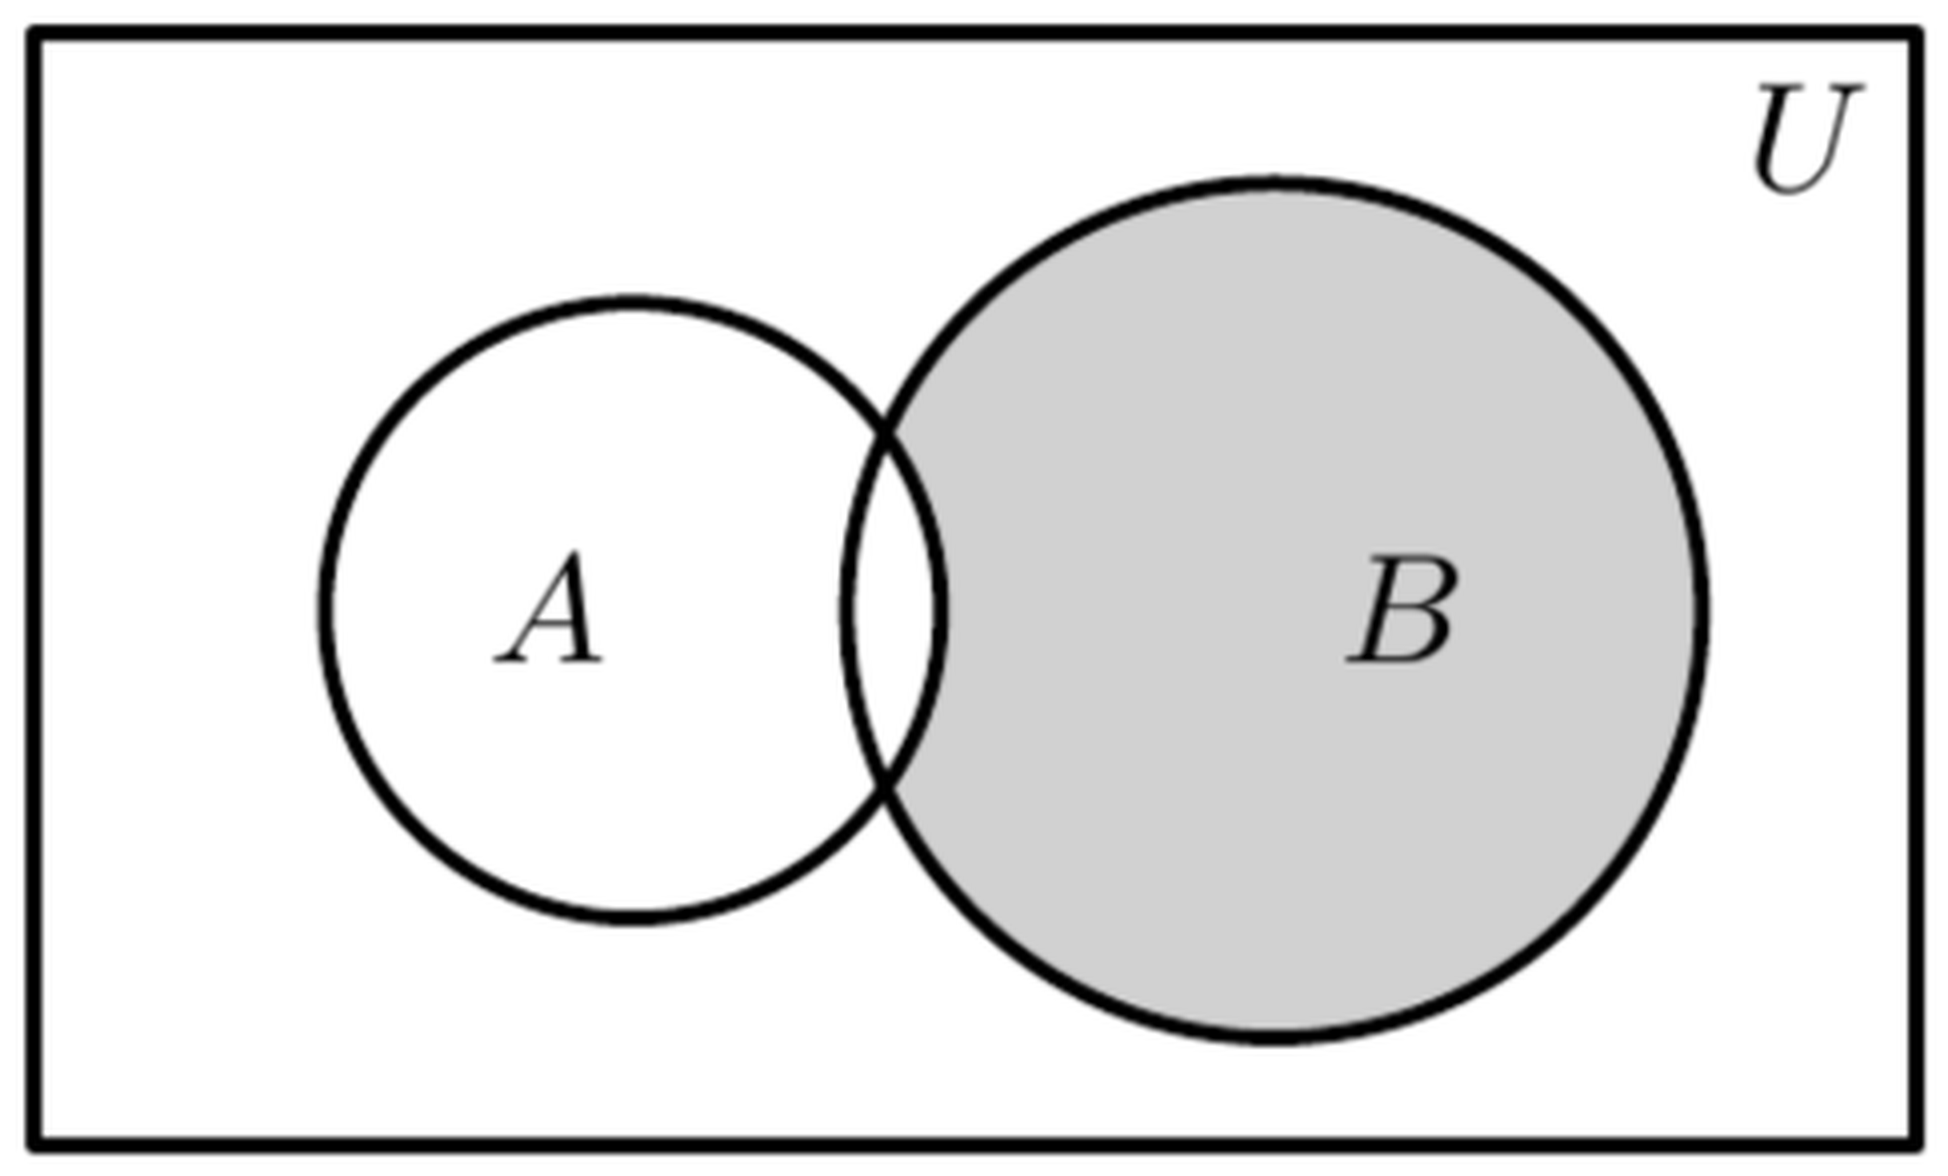
\includegraphics[width=0.38\textwidth]{figures/gao160_q4.png}
\end{center}

\ifanswer
\solbegin
\step{阴影部分表示 $B\cap\overline{A}=\{1,2\}$.}
\solend
\fi

% === Q5 === "图像"（有亻）照录；解析 1 行
\item 已知常数 $a>0$ 且 $a\ne1$，假设无论 $a$ 取何值，函数 $y=\log_a(5x-9)-4$ 的图像恒过一个定点，则这个定点的坐标为\blankline[4.4em].

\ifanswer
\solbegin
\step{$5x-9=1\Rightarrow x=2$，此时 $y=\log_a 1-4=-4$，定点为 $(2,-4)$.}
\solend
\fi

% === Q6 === 解析 2 行
\item 不等式 $(1-2x)^{\frac{3}{4}}>x^{\frac{3}{4}}$ 的解集为\blankline[4.4em].

\ifanswer
\solbegin
\step{定义域为 $\left[0,\dfrac{1}{2}\right]$，由幂函数的单调性，原不等式等价于 $1-2x>x$，}
\step{得 $0\leqslant x<\dfrac{1}{3}$，故解集为 $\left[0,\dfrac{1}{3}\right)$.}
\solend
\fi

% === Q7 === 绝对值 \lvert…\rvert；解析 2 行（跨 01—02 页）
\item 已知不等式 $\lvert x+3\rvert+\lvert x-2\rvert\geqslant 5$，当其等号成立时，$x$ 的取值范围是\blankline[4.4em].

\ifanswer
\solbegin
\step{$\lvert x+3\rvert+\lvert x-2\rvert=\lvert x+3\rvert+\lvert 2-x\rvert\geqslant\lvert(x+3)+(2-x)\rvert=5$，}
\step{等号成立当且仅当 $(x+3)(2-x)\geqslant0$，即 $x\in[-3,2]$.}
\solend
\fi

% === Q8 === 解析 4 行
\item 已知函数 $f(x)=\lvert\log_2 x\rvert$，若方程 $f(x)-t=0$ 有两个不同的实数根 $x_1,x_2$，则 $x_1+x_2$ 的取值范围是\blankline[4.4em].

\ifanswer
\solbegin
\step{方程有两个不同实根，必有 $t>0$，两根为 $2^t,2^{-t}$，}
\step{所以 $x_1+x_2=2^t+2^{-t}>2$（等号仅在 $t=0$ 时成立）.}
\step{任取 $s>2$，令 $a=\dfrac{s+\sqrt{s^2-4}}{2}>1$，取 $t=\log_2 a>0$，则 $x_1+x_2=a+\dfrac{1}{a}=s$，}
\step{所以取值范围为 $(2,+\infty)$.}
\solend
\fi

% === Q9 === 中文弯引号、\R、绝对值 \lvert…\rvert；解析 4 行
\item 已知 $a\in\R$，$b\in\R$，$p:\dfrac{1}{\lvert a\rvert}>\dfrac{1}{\lvert b\rvert}$，$q:\dfrac{1}{a}>\dfrac{1}{b}$，则 $p$ 是 $q$\blankline[4.4em]条件（用“充分非必要”、“必要非充分”、“充要”或“既非充分又非必要”填空）.

\ifanswer
\solbegin
\step{由 $p$、$q$ 中的分式有意义，$a\ne0$ 且 $b\ne0$.}
\step{当 $a=-1,b=-2$ 时，$p$ 成立而 $q$ 不成立，故 $p$ 不是 $q$ 的充分条件.}
\step{当 $a=1,b=-1$ 时，$q$ 成立而 $p$ 不成立，故 $p$ 不是 $q$ 的必要条件.}
\step{故 $p$ 是 $q$ 的充分非必要条件.}
\solend
\fi

% === Q10 === 解析 3 行；其后独立【注】按语 5 行（见头注 ② ⑯、⑤ 1）
\item 已知常数 $a>0$，函数 $y=\dfrac{2^x}{2^x+ax}$ 的图像经过点 $P\left(p,\dfrac{5}{6}\right)$、$Q\left(q,\dfrac{1}{6}\right)$，若 $2^{p+q}=3pq$，则 $a=$\blankline[4.4em].

\ifanswer
\solbegin
\step{由 $\dfrac{2^p}{2^p+ap}=\dfrac{5}{6}$ 得 $2^p=5ap$；由 $\dfrac{2^q}{2^q+aq}=\dfrac{1}{6}$ 得 $2^q=\dfrac{aq}{5}$.}
\step{$2^p>0$，$2^q>0$，$a>0$，得 $p>0$，$q>0$.}
\step{两式相乘得 $2^{p+q}=a^2pq$，又 $2^{p+q}=3pq$ 且 $pq\ne0$，故 $a^2=3$，$a=\sqrt{3}$.}
\solend
% 【注】按语（讲评版编者按，5 个印刷行，仅答案版出，不属于任何题的【解析】）
\stepm{【注】}{按原卷数据严格推敲，点 $Q$ 其实不存在：$a=\sqrt{3}$ 时 $2^q=\dfrac{\sqrt{3}}{5}q<q$；而当 $q>0$}
\step{时，取非负整数 $n$ 使 $n\leqslant q<n+1$，由 $2^{k+1}=2^k+2^k\geqslant2^k+1$ 逐次推得 $2^n\geqslant n+1$，于是}
\step{$2^q\geqslant2^n\geqslant n+1>q$，矛盾. 所以题设条件互相矛盾，严格说本题无解；$\sqrt{3}$ 是由题给关}
\step{系直接推出的值，按命题意图作为答案. 原卷数据疑似有误（同型常见题为 $P\left(p,\dfrac{6}{5}\right)$、}
\step{$Q\left(q,-\dfrac{1}{5}\right)$、$2^{p+q}=36pq$，得 $a=6$）.}% 见头注 ⑤ 1，照录未改
\fi

% === Q11 === 纳皮尔对数材料题；\Z、大数；解析 6 行
\item 17 世纪初，约翰·纳皮尔为了简化计算而发明了对数. 对数的发明是数学史上的重大事件，恩格斯曾经把笛卡尔的坐标系、纳皮尔的对数、牛顿和莱布尼兹的微积分共同称为 17 世纪的三大数学发明. 我们知道，任何一个正实数 $N$ 可以表示成 $N=a\times10^n$ ($1\leqslant a<10,n\in\Z$) 的形式，这便是科学记数法，若两边取常用对数，有 $\lg N=n+\lg a$，则可以估计 $3^{2026}$ 的最高位上的数值为\blankline[4.4em].

\ifanswer
\solbegin
\step{设 $3^{2026}=a\times10^n$ ($1\leqslant a<10,n\in\Z$)，则 $2026\lg 3=n+\lg a$.}
\step{用 $\lg 3\approx 0.4771$ 粗估，得 $2026\lg 3\approx 966.60$.}
\step{为核验误差，用 $0.47712<\lg 3<0.47713$，}
\step{得 $966.64512<2026\lg 3<966.66538$，因此 $n=966$.}
\step{于是 $\lg 4\approx 0.60206<0.64512<\lg a<0.66538<\lg 5\approx 0.69897$，}
\step{所以 $4<a<5$，最高位为 4，估算误差不影响结论.}
\solend
\fi

% === Q12 === 自定义"性质 P"；文本圈数字①②③；解析 19 行（跨 03—05 页）
\item 对于数集 $X=\{-1,x_1,x_2,x_3,\cdots,x_n\}$，其中 $0<x_1<x_2<x_3<\cdots<x_n$，$n\geqslant2$，定义点集 $Y=\{(s,t)\mid s\in X,t\in X\}$，若对于任意 $(s_1,t_1)\in Y$，存在 $(s_2,t_2)\in Y$，使得 $s_1s_2+t_1t_2=0$，则称集合 $X$ 具有性质 $P$. 则下列命题中为真命题的是\blankline[4.4em].

① $X=\{-1,1,2\}$ 具有性质 $P$；②若集合 $X$ 具有性质 $P$，则 $1\in X$；

③集合 $X$ 具有性质 $P$，若 $x_1=\dfrac{1}{2}$，则 $x_n=2$.

\ifanswer
\solbegin
\step{因为 $X=\{-1,1,2\}$，}
\step{所以 $Y=\{(-1,-1),(1,1),(2,2),(-1,1),(-1,2),(1,-1),(1,2),(2,-1),(2,1)\}$，}
\step{由集合 $X$ 具有性质 $P$ 的定义，对于任意 $(s,t)\in Y$，}
\step{若 $s>0$，$t>0$，则 $s=t$ 或 $(s,t)=(1,2)$ 或 $(s,t)=(2,1)$，}
\step{若 $s=t$，取 $s_2=-1$，$t_2=-1$，则 $ss_2+tt_2=0$；}
\step{若 $(s,t)=(1,2)$，取 $s_2=2$，$t_2=-1$，则 $ss_2+tt_2=0$；}
\step{若 $(s,t)=(2,1)$，取 $s_2=-1$，$t_2=2$，则 $ss_2+tt_2=0$；}
\step{若 $s$、$t$ 有一个为负数，则 $s=-1$ 或 $t=-1$，}
\step{若 $s=-1$，则取 $s_2=t$，$t_2=1$，则 $ss_2+tt_2=0$；}
\step{若 $t=-1$，则取 $s_2=1$，$t_2=s$，则 $ss_2+tt_2=0$；故①正确；}
\step{对于任意 $(s_1,t_1)\in Y$，存在 $(s_2,t_2)\in Y$，使得 $s_1s_2+t_1t_2=0$，}
\step{取 $(x_1,x_1)\in Y$，存在 $(x_p,x_q)$ 使得 $x_1x_p+x_1x_q=0$，所以 $x_p+x_q=0$，}
\step{不妨设 $x_p=1$，$x_q=-1$，所以若集合 $X$ 具有性质 $P$，则 $1\in X$，故②正确；}
\step{③假设 $x_n>1$，令 $s_1=\dfrac{1}{2},t_1=x_n$，则存在 $s$、$t\in X$ 使得 $\dfrac{1}{2}s+tx_n=0$，}
\step{同②得 $s$、$t$ 中必有一个数为 $-1$，}
\step{若 $s=-1$，则 $tx_n=\dfrac{1}{2}$，于是 $t=\dfrac{1}{2x_n}<\dfrac{1}{2}=x_1$，矛盾，}
\step{若 $t=-1$，则 $\dfrac{1}{2}s=x_n\cdot(-1)$，于是 $s=2x_n>x_n$，也矛盾，}% 原卷如此（与结论符号不自洽），照录未改，见头注 ⑤ 2
\step{所以 $x_n\leqslant1$，又由②得 $1\in X$，所以 $x_n\geqslant1$，所以 $x_n=1$，故③错误，}
\step{故真命题是①②.}
\solend
\fi

\end{enumerate}

% 答案版里填空解析把页排满，节标题会落到页末、与第 13 题分家（切页审计 B 类）；
% 守卫放 \bigsec 之前，连节标题一起量页高（高一157 成例）
\needvspace{7cm}
\bigsec{二、选择题}

\begin{enumerate}
\setcounter{enumi}{12}

% === Q13 === "图像"照录；解析 1 行，故选 $B$
\item 下列函数中，图像与函数 $y=3^x$ 图像关于 $y$ 轴对称的是\mbox{（\quad）}

\keepwithprev
A. $y=x^3$\qquad B. $y=\left(\dfrac{1}{3}\right)^x$\qquad C. $y=-3^x$\qquad D. $y=\log_3 x$

\ifanswer
\solbegin
\step{将 $x$ 换为 $-x$，得对称图像对应的函数为 $y=3^{-x}=\left(\dfrac{1}{3}\right)^x$，故选 $B$.}
\solend
\fi

% === Q14 === 中文弯引号；解析 2 行（跨 05 页上下），故选 $B$
\item 命题“存在 $x\in(1,+\infty)$，使得 $f(x)>0$”的否定形式为\mbox{（\quad）}

\keepwithprev
A. 不存在 $x\in(-\infty,1]$，使得 $f(x)>0$\qquad B. 对任意 $x\in(1,+\infty)$，有 $f(x)\leqslant0$

C. 对任意 $x\in(-\infty,1]$，有 $f(x)\leqslant0$\qquad D. 存在 $x\in(1,+\infty)$，使得 $f(x)\leqslant0$

\ifanswer
\solbegin
\step{将“存在”改为“对任意”，$x$ 的范围不变，并将 $f(x)>0$ 否定为 $f(x)\leqslant0$，}
\step{故选 $B$.}
\solend
\fi

% === Q15 === \R；四选项两行；解析 3 行，故选 $D$
\item 设 $a>0$，$s\in\R$. 下列各项中，能推出 $a^s>a$ 的一项是\mbox{（\quad）}

\keepwithprev
A. $a>1$，且 $s>0$\qquad B. $a>1$，且 $s<0$

C. $0<a<1$，且 $s>0$\qquad D. $0<a<1$，且 $s<0$

\ifanswer
\solbegin
\step{当 $a>1$ 时，$a^s>a\Leftrightarrow s>1$，A、B 均不能保证.}
\step{当 $0<a<1$ 时，$a^s>a\Leftrightarrow s<1$，C 不能保证，D 中 $s<0<1$，满足要求；}
\step{故选 $D$.}
\solend
\fi

% === Q16 === 题目配图（三版都出）；几何符号 \triangle ABC；解析 3 行，故选 $C$
\needvspace{8cm}
\item 数学说明的方法多种多样，其中利用图形说明就是一种重要方法. 如图所示，在等腰直角三角形 $\triangle ABC$ 中，点 $O$ 为斜边 $AB$ 的中点，点 $D$ 为斜边 $AB$ 上异于顶点的一个动点，设 $AD=a$，$BD=b$，则可用该图形能说明的不等式为\mbox{（\quad）}

\begin{center}
% Q16 等腰直角三角形 ABC 图（C/A/O/D/B 标注）取 05 页右下，去粉色水印、去色、3× LANCZOS 放大；三版都出
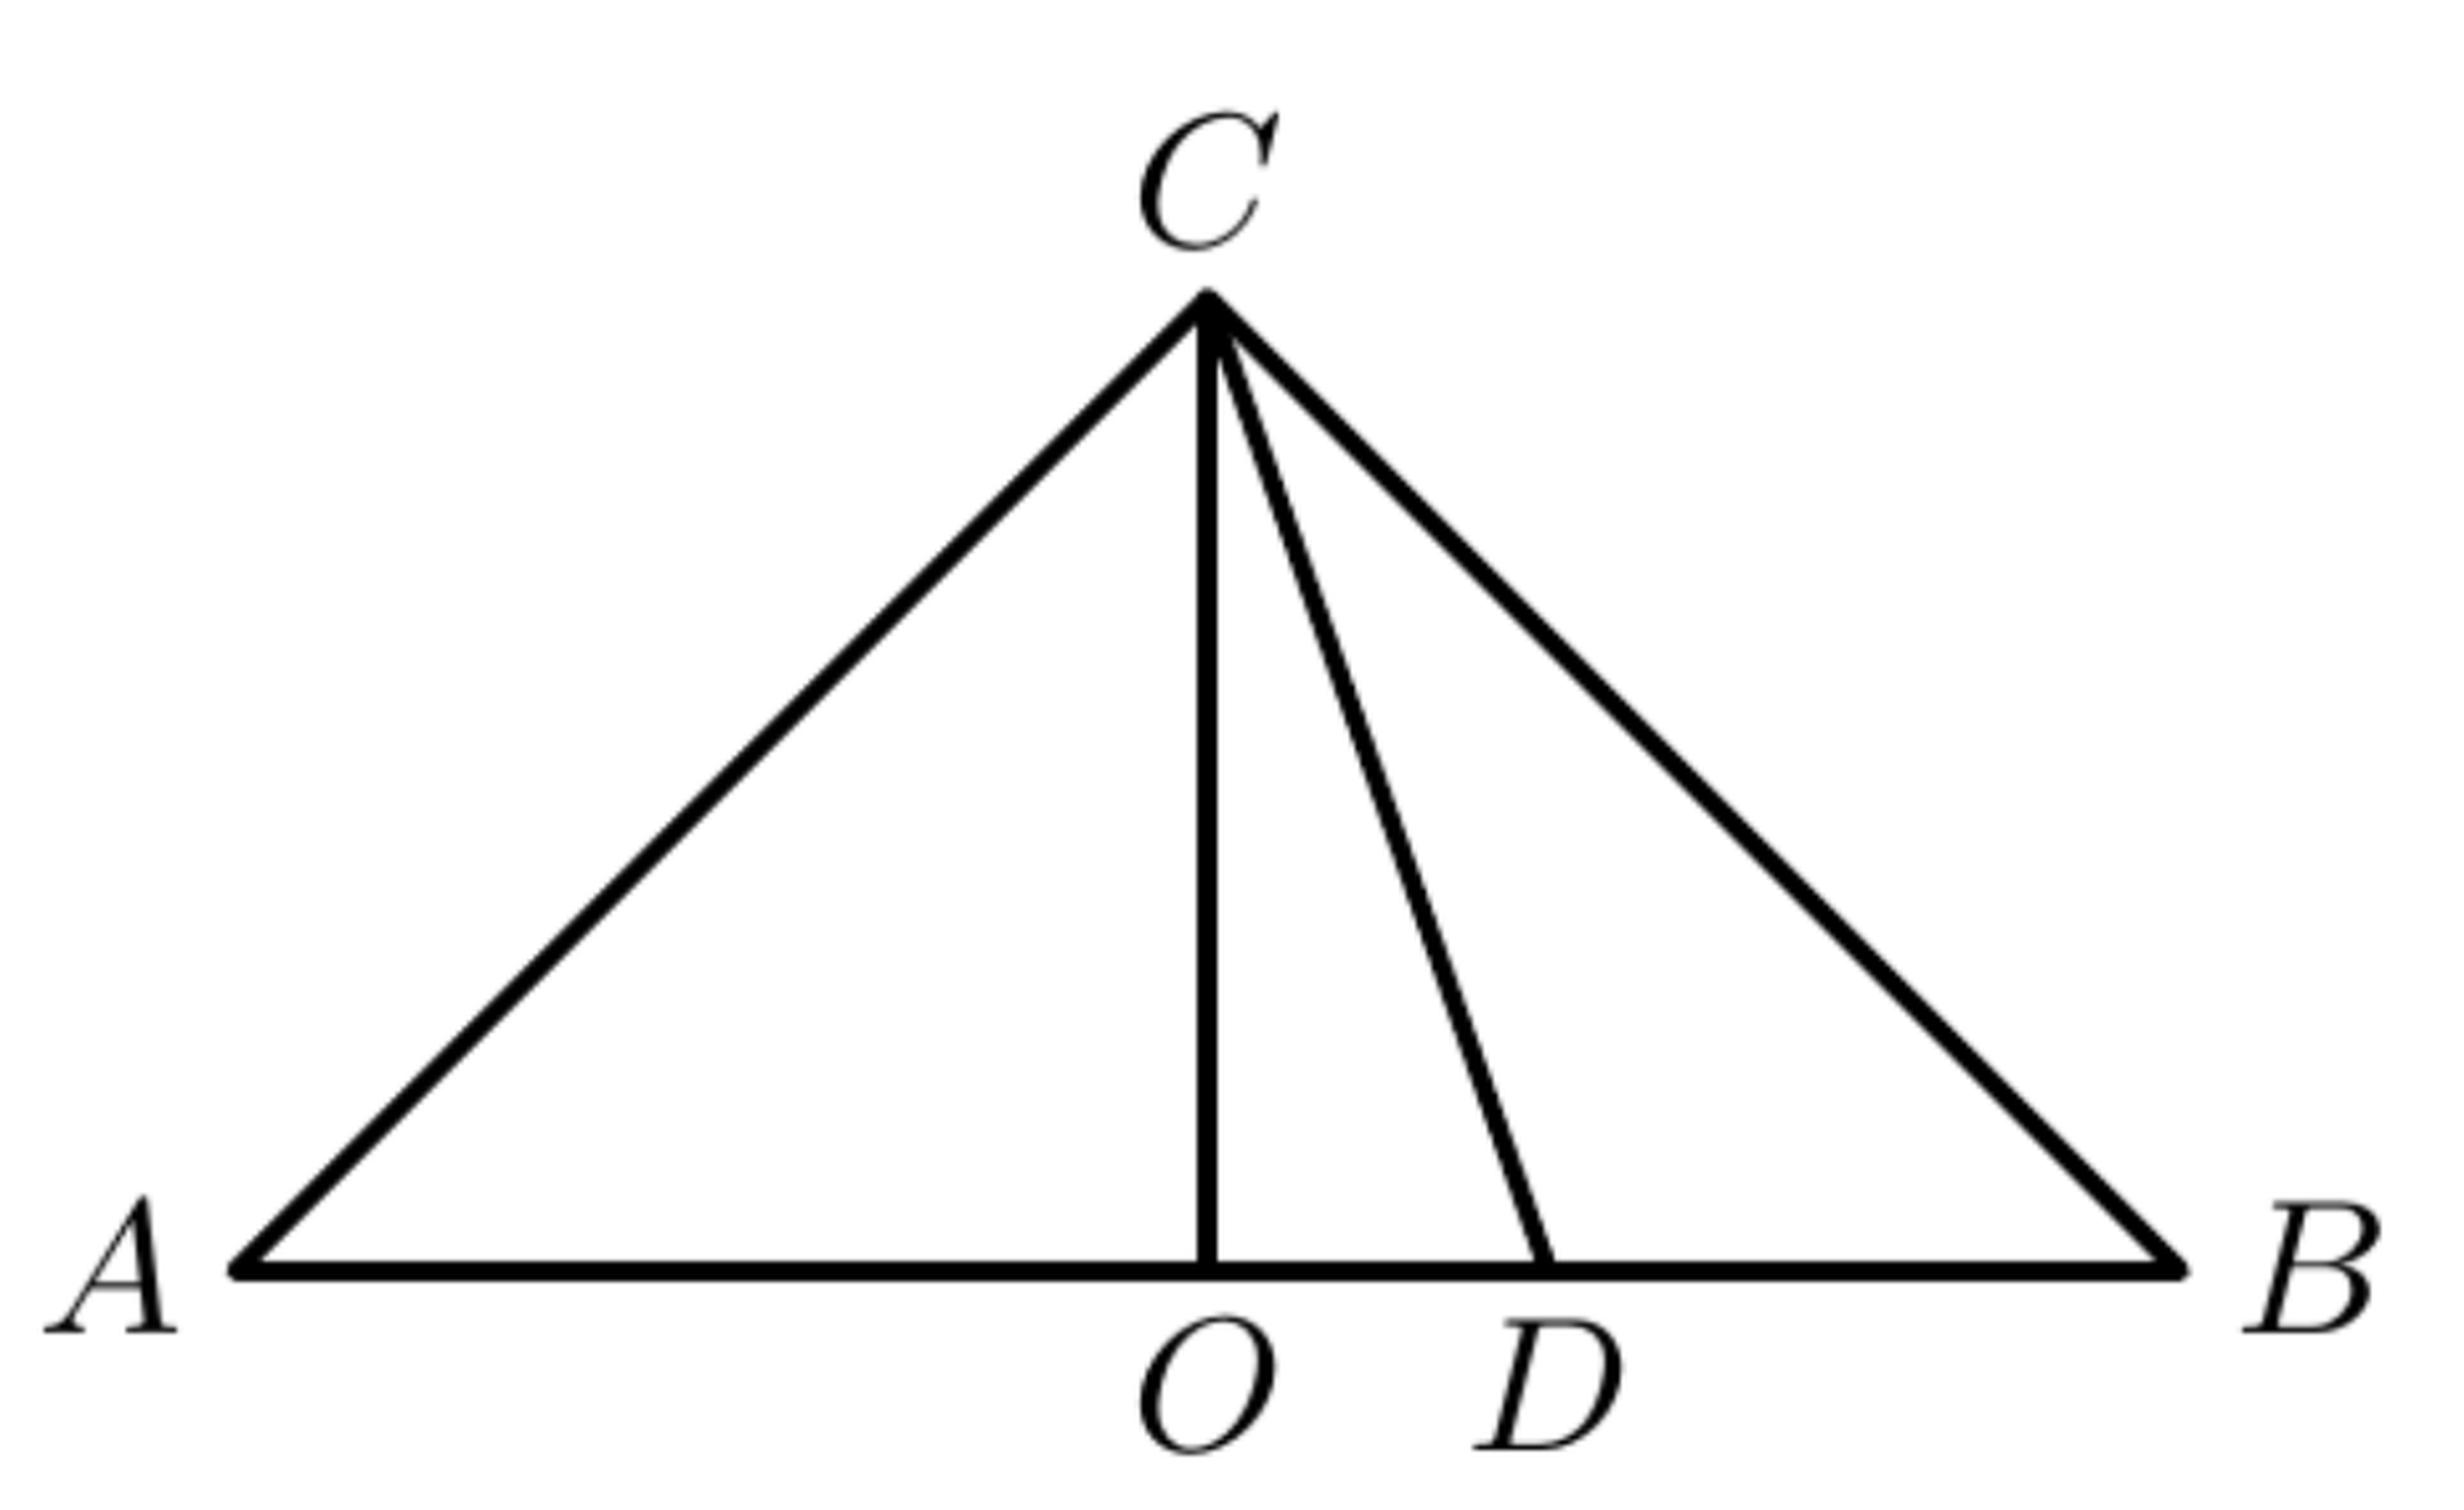
\includegraphics[width=0.34\textwidth]{figures/gao160_q16.png}
\end{center}

\keepwithprev
A. $\dfrac{a+b}{2}\geqslant\sqrt{ab}$ ($a>0,b>0$)\qquad B. $a^2+b^2\geqslant2\sqrt{ab}$ ($a>0,b>0$)

C. $\dfrac{a+b}{2}\leqslant\sqrt{\dfrac{a^2+b^2}{2}}$ ($a>0,b>0$)\qquad D. $\dfrac{2ab}{a+b}\leqslant\sqrt{ab}$ ($a>0,b>0$)

\ifanswer
\solbegin
\step{$CO=AO=\dfrac{a+b}{2},OD=\left\lvert a-\dfrac{a+b}{2}\right\rvert=\dfrac{\lvert a-b\rvert}{2}$，}
\step{$CD=\sqrt{CO^2+OD^2}=\sqrt{\dfrac{a^2+b^2}{2}}\geqslant CO=\dfrac{a+b}{2}$，}
\step{等号当且仅当 $a=b$ 时成立，故选 $C$.}
\solend
\fi

\end{enumerate}

\bigsec{三、解答题}

\begin{enumerate}
\setcounter{enumi}{16}

% === Q17 === cases 块算一行；判别式印等腰偏高三角 \Delta；解析 7 行
\item 已知幂函数 $f(x)=(m^2-2m-2)x^{m-1}$ 在 $(0,+\infty)$ 上是严格增函数.

(1) 求 $m$ 的值；

(2) 若关于 $x$ 的方程 $f(x)=(t+1)x-t^2$ 有两个不相等的正实根，求实数 $t$ 的取值范围.

\ifanswer
\solbegin
\step{(1) 幂函数的系数为 1，因此 $m^2-2m-2=1\Leftrightarrow(m-3)(m+1)=0$，}
\step{解得 $m=3$ 或 $m=-1$.}
\step{由 $f(x)$ 在 $(0,+\infty)$ 上严格递增，得 $m-1>0$，所以 $m=3$，}
\step{此时 $f(x)=x^2$.}
\step{(2) 原方程化为 $x^2-(t+1)x+t^2=0$，}
\step{方程有两个不相等的正实根，则 $\begin{cases}\Delta=(t+1)^2-4t^2=(1-t)(3t+1)>0\\t+1>0\\t^2>0\end{cases}$，}% 判别式原卷印等腰偏高三角 \Delta，照录
\step{得 $t\in\left(-\dfrac{1}{3},0\right)\cup(0,1)$.}
\solend
\fi

% === Q18 === 补集上划线 \overline{A}、\subseteq 带下划线、\varnothing；解析 8 行
\item 已知集合 $A=\{x\mid\lvert x-a\rvert<a-3\}$，$B=\left\{x\mid\dfrac{x+1}{x-2}\geqslant2\right\}$.

(1) 若 $a=5$，求 $\overline{A}\cap B$；

(2) 若 $A\cap B=A$，求实数 $a$ 的取值范围.

\ifanswer
\solbegin
\step{(1) $\dfrac{x+1}{x-2}\geqslant2\Leftrightarrow\dfrac{5-x}{x-2}\geqslant0\Leftrightarrow2<x\leqslant5,B=(2,5]$，}
\step{当 $a=5$ 时，$A=\{x\mid\lvert x-5\rvert<2\}=(3,7)$，于是 $\overline{A}=(-\infty,3]\cup[7,+\infty)$，}
\step{因此 $\overline{A}\cap B=(2,3]$.}
\step{(2) $A\cap B=A$ 等价于 $A\subseteq B$.}
\step{当 $a\leqslant3$ 时，$a-3\leqslant0$，$A=\varnothing$，满足条件.}
\step{当 $a>3$ 时，$\lvert x-a\rvert<a-3\Leftrightarrow3<x<2a-3,A=(3,2a-3)$，}
\step{此时 $A\subseteq B=(2,5]$ 等价于 $2a-3\leqslant5$，即 $a\leqslant4$，结合 $a>3$ 得 $3<a\leqslant4$.}
\step{合并两种情形，实数 $a$ 的取值范围为 $(-\infty,4]$.}
\solend
\fi

% === Q19 === 数据表 tabular 重排（高一130 成例）；cases 块算一行；解析 6 行
\item 作为我国最高水平的综合性运动会，全运会汇聚了国内顶尖体育健儿，某代表队从第 8 届全运会开始登上赛场，且参赛运动员人数逐年递增. 设 $t$ 为该代表队参赛后经过的届数，即第 8 届为 $t=0$，第 9 届为 $t=1$，以此类推. 经过 $t$ 届，运动员人数为 $y$ 人，具体数据如下：

\begin{center}
\begin{tabular}{cccccc}
$t$ & 0 & 1 & 2 & 3 & 4 \\
\hline
届数 & 8 & 9 & 10 & 11 & 12 \\
运动员人数（$y$ 人） & 4 & 11 & 25 & 53 & 109
\end{tabular}
\end{center}

(1) 现有以下两种函数模型：① $y=a\cdot b^t+c$ ($a>0,b>1$)；② $y=\log_a(t+b)+c$ ($b>0,a>1$). 请根据上表中运动员人数的增长规律，选出你认为符合的函数模型（不用说明理由），并利用表中前 3 组数据求出相应的函数解析式；

(2) 若参赛运动员人数按照 (1) 中求得的模型继续增长，在第几届全运会时，该代表队运动员人数将会首次超过 1000 人？

\ifanswer
\solbegin
\step{(1) 选模型①，将前 3 组数据代入，得 $\begin{cases}a+c=4\\ab+c=11\\ab^2+c=25\end{cases}$，}% 原卷印"选模型①"（圈数字①），OCR 误作"四"，照录①，见头注 ⑤ 3
\step{相邻两式相减，得 $a(b-1)=7$，$ab(b-1)=14$，}
\step{两式相除得 $b=2$，进而 $a=7$，$c=-3$，所求函数解析式为 $y=7\cdot2^t-3$.}
\step{(2) $y=7\cdot2^t-3$ 随 $t$ 的增大而增大，且 $t=7$ 时，$y=893<1000$；}
\step{$t=8$ 时，$y=1789>1000$，}
\step{$t$ 为非负整数，首次超过 1000 人时 $t=8$，对应第 $8+8=16$ 届全运会.}
\solend
\fi

% === Q20 === 解析 12 行（跨 08—09 页）
\item 已知函数 $f(x)=\log_a(a-a^x)$.

(1) 求该函数的定义域；

(2) 若 $a>1$，试判断关于 $x$ 的方程 $f(x)=2$ 是否有实数解，并说明理由；

(3) 若当 $x\in(-\infty,0]$ 时，关于 $x$ 的不等式 $f(x)\geqslant-1$ 恒成立，求实数 $a$ 的取值范围.

\ifanswer
\solbegin
\step{(1) 对数的底数须满足 $a>0$ 且 $a\ne1$，真数须满足 $a-a^x>0$，即 $a^x<a^1$.}% 原卷印 $a^1$，照录未化简，见头注 ⑤ 4
\step{当 $a>1$ 时，$x<1$，定义域为 $(-\infty,1)$.}
\step{当 $0<a<1$ 时，$x>1$，定义域为 $(1,+\infty)$.}
\step{(2) 当 $a>1$ 时，若 $f(x)=2$，则 $a-a^x=a^2\Rightarrow a^x=a(1-a)<0$，}
\step{这与 $a^x>0$ 矛盾，因此方程无实数解.}
\step{(3) 不等式在 $(-\infty,0]$ 上恒成立，须先保证该区间包含于函数的定义域，}
\step{由 (1) 得 $a>1$.}
\step{当 $x\leqslant0$ 时，$0<a^x\leqslant1$，所以 $a-a^x\geqslant a-1>0$.}
\step{由对数函数的单调性，$f(x)=\log_a(a-a^x)\geqslant\log_a(a-1)=f(0)$，}
\step{等号当且仅当 $x=0$ 时成立，}
\step{因此所求条件等价于 $\log_a(a-1)\geqslant-1\Leftrightarrow a-1\geqslant\dfrac{1}{a}\Leftrightarrow a^2-a-1\geqslant0$，}
\step{结合 $a>1$，得 $a\in\left[\dfrac{1+\sqrt{5}}{2},+\infty\right)$.}
\solend
\fi

% === Q21 === "和积平衡集"定义证明题；\N；解析 18 行（跨 09—10 页）
\item 已知有限集 $A=\{a_1,a_2,\cdots,a_n\}$ ($n\geqslant2,n\in\N$)，如果 $A$ 中元素 $a_i$ ($i=1,2,3,\cdots,n$) 满足 $a_1+a_2+a_3+\cdots+a_n=a_1\times a_2\times\cdots\times a_n$，就称 $A$ 为“和积平衡集”.

(1) 分别判断集合 $A=\{1,2,3,4\}$，$B=\{4+2\sqrt{2},4-2\sqrt{2}\}$ 是否为“和积平衡集”；

(2) 已知 $a_1$、$a_2$ 是两个不同的正数，且 $\{a_1,a_2\}$ 是“和积平衡集”，请用反证法证明：$a_1$、$a_2$ 至少有一个大于 2；

(3) 若 $a_i\geqslant1$，且 $a_i\in\N$，求所有符合条件的“和积平衡集”.

\ifanswer
\solbegin
\step{(1) 因为 $1+2+3+4=10\ne24=1\times2\times3\times4$，所以 $A$ 不是“和积平衡集”.}
\step{因为 $(4+2\sqrt{2})+(4-2\sqrt{2})=8=(4+2\sqrt{2})(4-2\sqrt{2})$，}
\step{所以 $B$ 是“和积平衡集”.}
\step{(2) 假设 $a_1$、$a_2$ 都不大于 2，则 $\dfrac{1}{a_1}\geqslant\dfrac{1}{2},\dfrac{1}{a_2}\geqslant\dfrac{1}{2}$，}
\step{由于 $a_1\ne a_2$，上述两个不等式至少有一个严格成立.}
\step{而 $a_1+a_2=a_1a_2$，两边除以 $a_1a_2>0$，得 $1=\dfrac{1}{a_1}+\dfrac{1}{a_2}>\dfrac{1}{2}+\dfrac{1}{2}=1$，矛盾，}
\step{所以 $a_1$、$a_2$ 至少有一个大于 2.}
\step{(3) 不妨设 $a_1<a_2<\cdots<a_n$，由各元素均为正整数，得 $a_i\geqslant i$.}
\step{若 $n\geqslant4$，因其余因子均不小于 1，}
\step{有 $a_1a_2\cdots a_n\geqslant a_2a_{n-1}a_n\geqslant2(n-1)a_n>na_n>a_1+a_2+\cdots+a_n$，}
\step{与和积平衡条件矛盾，因此只需讨论 $n=2,3$.}
\step{当 $n=2$ 时，$a_1+a_2=a_1a_2\Leftrightarrow(a_1-1)(a_2-1)=1$，}
\step{两个因子均为非负整数，只能有 $a_1=a_2=2$，与元素互不相同矛盾.}
\step{当 $n=3$ 时，若 $a_1\geqslant2$，则 $a_2\geqslant3$，从而 $a_1a_2a_3\geqslant6a_3>3a_3>a_1+a_2+a_3$，}
\step{矛盾，因此 $a_1=1$.}
\step{此时 $1+a_2+a_3=a_2a_3\Leftrightarrow(a_2-1)(a_3-1)=2$，}
\step{由 $1\leqslant a_2-1<a_3-1$，得 $a_2-1=1$、$a_3-1=2$，即 $a_2=2$、$a_3=3$.}
\step{检验 $1+2+3=1\times2\times3=6$，所求集合为 $\{1,2,3\}$.}
\solend
\fi

\end{enumerate}

\end{document}
"
%
% ① 原始材料：微信公众号"魔都数学加油站"文章，连载"27学年高一160"，原卷卷面标题
% "2026-2027 年奉贤中学高一上期中"（卷面未印副标题、未印连载号）。
% 正文为 10 张 PNG 页（01/04/10 为 2560×3620，02/03/05/06/07/08/09 为
% 4762×6735，同一篇各页分辨率混排，逐页按各自分辨率裁图核对）。
% 体例：讲评版——填空 3—12（10 题）、选择 13—16（4 题）、解答 17—21（5 题），
% 共 19 题，自第 3 题起编（1、2 未印在本篇）；19 题逐题印【解析】，无只印【答案】
% 的题；四道选择题答案在解析末句"故选 $B$/$B$/$D$/$C$"，题干括号
% \mbox{（\quad）} 留空、不另提 \ans{}。题目、答案、解析均据原图转录；卷面粉红色
% 水印"魔都数学加油站"及公众号页脚未录入。
% 全卷插图清单（逐页通读 10 页确认）：2 幅，均为题目配图、三版都出——
%   · Q4 韦恩图（01 页右侧：矩形全集 U、两圆 A/B、阴影部分 B∩上划线 A、
%     标注 U/A/B），裁 figures/gao160_q4.png；
%   · Q16 等腰直角三角形 ABC 图（05 页右下：C 顶点、A/O/D/B 共线底边、
%     CO 与 CD 两条线段），裁 figures/gao160_q16.png；
%   两图均取原卷截图 3—4× LANCZOS 放大、去粉色水印、转灰度、autocontrast；
%   Q4 图左侧题干残字"示"、Q16 图左侧题干残字均已裁白。
%   Q19 有一张 3 行数据表（t／届数／运动员人数（y 人），t=0..4），按全稿
%   成例（高一130）用 tabular 重排，不做成 png；其余各页无题目配图、
%   无解析内配图、无其它表格、无"如图"处。
%
% 卷首标题：原卷印作"2026-2027 年奉贤中学高一上期中"，年份区间按全稿惯例排 en dash；
% 原卷卷面未印副标题，本稿按同期中卷知识模块口径补出"集合与常用逻辑用语、不等式、函数"。
%
% ② 与原卷的排版差异／照录项清单：
%   ① 原文从第 3 题起，本稿保留原题号；共 19 题三节，解答题 5 题到 21；
%      三节各自一个 enumerate + \setcounter{enumi}{2}/{12}/{16}（不贯穿），
%      用 \examtitlest[3] 起手；
%   ② 混合体例说明：19 题全印【解析】、用 \solbegin…\solend，无只印【答案】
%      或答案印括号内的题；四道选择题答案在解析末句"故选 $B$/$B$/$D$/$C$"
%      （逐个放大复核）、括号 \mbox{（\quad）} 留空、不另提 \ans{}；答案版
%      【答案】/【解析】标记数 = 19 = 全卷题数（0 个 \ans ＋ 19 个 \solbegin）；
%   ③ 原卷卷面未印副标题，本稿按知识模块口径补出；
%   ④ 原卷填空横线按全稿惯例排 \blankline[4.4em]；选择题括号排 \mbox{（\quad）}、
%      四道选择题的选项段前按惯例各加 \keepwithprev；解答题不留作答区、不加
%      \anspace（原卷为讲评版，109—113 起全稿不用 \anspace）；
%   ⑤ 数集归一：Q4"$U=\Z$"、Q9"$a\in\R$，$b\in\R$"、Q11"$n\in\Z$"、
%      Q15"$s\in\R$"、Q21"$n\in\N$""$a_i\in\N$"原卷印正体粗体 Z/R/N，
%      按全稿惯例归一 \Z／\R／\N；集合描述竖线排 \mid（Q3、Q4、Q12、
%      Q18、Q21）；空集 \varnothing（Q18 解析 (2)）；补集照原卷上划线排
%      \overline{A}（Q4 解析、Q18 (1) 题干与解析）；子集符号 Q18 两处
%      "$A\subseteq B$"印带下划线 ⊆、照录 \subseteq；
%   ⑥ 绝对值排 \lvert…\rvert（Q7、Q8 题干与解析、Q9 题干、Q16 解析、
%      Q18 题干与解析），Q16 解析的 \left\lvert…\right\rvert 与 \lvert…\rvert
%      均在同一 $…$ 组内配对平衡；
%   ⑦ 判别式两形混用逐处照录不统一（放大逐处确认）：Q3 解析
%      "$\triangle=1^2-4a\times\frac{1}{4}=0$"原卷印扁等边三角、照录
%      \triangle；Q17 解析 cases 块"$\Delta=(t+1)^2-4t^2=(1-t)(3t+1)>0$"
%      原卷印等腰偏高三角、照录 \Delta；Q16 题干几何符号"$\triangle ABC$"
%      按全稿几何三角形记号惯例归一 \triangle（参照 高一150／132 成例）；
%   ⑧ 不等号按全稿惯例排 \leqslant／\geqslant；中文弯引号照录：Q9 题干
%      "充分非必要""必要非充分""充要""既非充分又非必要"、Q14 题干
%      "存在 $x\in(1,+\infty)$，使得 $f(x)>0$"与解析"存在""对任意"、
%      Q21 题干与解析多处"和积平衡集"；注释里一律 ASCII 引号；
%   ⑨ 文本圈数字逐处照录：Q12 题干①②③、Q12 解析"故①正确""同②得"
%      "故②正确""③假设""故③错误""故真命题是①②"、Q19 题干①②与解析
%      "选模型①"，均为印刷圈数字（非 \textcircled、非数学模式）；
%   ⑩ 半角逗号在数学组之间是全稿惯例、非笔误，逐处照录（Q8"$2^t,2^{-t}$"、
%      Q9"$a=-1,b=-2$""$a=1,b=-1$"、Q11"$1\leqslant a<10,n\in\Z$"、
%      Q12"$s_1=\frac{1}{2},t_1=x_n$"、Q16 选项"$a>0,b>0$"与解析
%      "$CO=AO=\frac{a+b}{2},OD=...$"、Q18"$2<x\leqslant5,B=(2,5]$"
%      "$3<x<2a-3,A=(3,2a-3)$"、Q21"$n=2,3$"等）；行中全角逗号／顿号
%      照录（Q15 选项"$a>1$，且 $s>0$"、Q12 解析"$s$、$t$"、Q21 解析
%      "$a_1$、$a_2$"），顿号一律移出数学模式；
%   ⑪ "图像／图象"逐处照录：本卷 Q5"的图像恒过一个定点"、Q10"的图像经过点"、
%      Q13 题干两处"图像"与解析"对称图像对应的函数"均印"图像"（有亻）；
%      Q16 印"图形"（利用图形说明、该图形能说明），无"图象"用例；
%   ⑫ 复杂式照录别简化：Q3 $ax^2+x+\frac14=0$、Q5 $y=\log_a(5x-9)-4$、
%      Q6 $(1-2x)^{\frac34}>x^{\frac34}$ 与 $\left[0,\frac12\right]$、
%      Q8 $\frac{s+\sqrt{s^2-4}}{2}$、Q10 $y=\frac{2^x}{2^x+ax}$ 与
%      $\frac{2^p}{2^p+ap}=\frac56$、$\frac{2^q}{2^q+aq}=\frac16$、
%      Q11 $N=a\times10^n$ 与 $3^{2026}$、$2026\lg3\approx966.60$、
%      $966.64512<2026\lg3<966.66538$、Q12 $Y=\{(s,t)\mid s\in X,t\in X\}$
%      与 $\frac12 s+tx_n=0$、Q16 $\sqrt{\frac{a^2+b^2}{2}}$、
%      Q17 $x^2-(t+1)x+t^2=0$ 与 $\left(-\frac13,0\right)\cup(0,1)$、
%      Q18 $\frac{5-x}{x-2}\geqslant0$、Q19 $y=a\cdot b^t+c$ 与
%      $y=\log_a(t+b)+c$、$y=7\cdot2^t-3$、Q20 $f(x)=\log_a(a-a^x)$
%      与 $a^2-a-1\geqslant0$、$\left[\frac{1+\sqrt5}{2},+\infty\right)$、
%      Q21 $4+2\sqrt2$ 与 $(a_2-1)(a_3-1)=2$ 等；
%   ⑬ 子题标号 (1)(2)(3) 按全稿惯例排半角括号；行末／行中句点按全稿惯例
%      排 ASCII `.`（不是全角「．」）；cases 块整体算一个印刷行
%      （Q17 解析、Q19 解析 (1)）；
%   ⑭ 配图：Q4／Q16 题目配图（三版都出）放 \item 内题干之后 \begin{center}，
%      各用 \needvspace{8cm} 守卫把整块推走，**守卫放在 \item 之前**
%      （见 高一153 Q11/Q19 成例与切页审计 B 类坑）；
%   ⑮ 一条 \step = 原卷解析的一个印刷行；跨上下半页的重叠行只算一次
%      （Q4 解析、Q9 解析首行、Q11 解析首行、Q12 解析"若 $s=-1$…"一行、
%      Q18 解析"此时 $A\subseteq B=(2,5]$…"一行、Q20 (2) 题干、
%      Q21 解析"由 $1\leqslant a_2-1<a_3-1$…"一行）；原卷折行别合并；
%   ⑯ Q10 之后另有一整块【注】按语（03 页上半，5 个印刷行），是讲评版作者对
%      原卷数据自相矛盾的加注、不属于任何题的【解析】。本稿按 高一53
%      "注：…"成例放 Q10 的 \solend 之后、Q10 的 \fi 收尾之前：
%      **整块只保留 Q10 那一层外层 \ifanswer**（那个 \fi 就是 Q10 的收尾），
%      块内 \stepm{【注】}{首行} ＋ 4 条 \step 各自自带内层 \ifanswer…\fi
%      （\step／\stepm 宏内自带，源码里不手动再包一层 \ifanswer，
%      否则 题目溯源.py 的 strip_answers 非贪婪正则会错切）；
%      \stepm 第一参数直接用「【注】」作标签，与全稿 \ans 的【答案】、
%      \solbegin 的【解析】同性质，未加粗以外不另加任何样式；
%      5 行仅答案版出、不新增 \item、不影响溯源，头注 ③ 单列登记、
%      不计入 19 题逐题 \step 账；\stepm 把【注】排成加粗着色标签
%      （原卷为黑色加粗），此一处着色差异在此登记；
%   ⑰ 原卷用字照录：Q11"约翰·纳皮尔""莱布尼兹"（原卷作"兹"，非通行"茨"）、
%      "17 世纪的三大数学发明"；Q16"数学说明的方法""点 $D$ 为斜边 $AB$ 上
%      异于顶点的一个动点"；Q19"登上赛场""以此类推"；
%
% ③ 行数复核：一条 \step = 原卷解析的一个印刷行，cases 块作一个印刷行计。
%   逐题数（逐页核对定稿）：Q3：5；Q4：1；Q5：1；Q6：2；Q7：2；Q8：4；
%   Q9：4；Q10：3；Q11：6；Q12：19；Q13：1；Q14：2；Q15：3；Q16：3；
%   Q17：7；Q18：8；Q19：6；Q20：12；Q21：18。
%   合计 107 条 \step（19 题逐题印刷行账），与原卷逐题印刷行相等。
%   **本卷源码 \step 总数 = 19 题逐题合计 107 ＋ Q10 后独立【注】块 5 行
%   = 112 行**（其中 \step 111 条、\stepm 1 条；\stepm 与 4 条 \step 合为
%   【注】块 5 印刷行）。该 5 行不计入「逐题印刷行」账，也不是任何题的
%   【解析】，而是讲评版编者按语；主会话核验脚本按全文统计 \step 时总数会
%   较逐题账多 5，已与主会话对齐、属已知预期而非错误。
%   全卷 19 题均设 \solbegin…\solend，答案版【答案】/【解析】标记数
%   = 19 = 全卷题数。
%
% ④ 页码分布（供回原图复核）：
%   卷首标题＋"一、填空题"＋Q3 题干＋解析 5 行＋Q4 题干＋韦恩图＋解析
%   1 行＋Q5 题干首行在 01 页上半；Q4 解析（重叠）＋Q5 题干续＋解析 1 行＋
%   Q6 题干＋解析 2 行＋Q7 题干＋解析首行在 01 页下半；Q7 解析末行＋
%   Q8 题干＋解析 4 行＋Q9 题干＋解析首行在 02 页上半；Q9 解析（重叠首行）
%   ＋余 3 行＋Q10 题干＋解析 3 行在 02 页下半；【注】按语 5 行＋Q11 题干＋
%   解析首行在 03 页上半；Q11 解析（重叠首行）＋余 5 行＋Q12 题干＋①②
%   在 03 页下半；Q12 ③＋解析前 9 行在 04 页上半；Q12 解析（重叠 2 行）
%   ＋余 8 行在 04 页下半；Q12 解析末 2 行＋"二、选择题"＋Q13 题干＋选项＋
%   解析 1 行＋Q14 题干＋选项＋解析首行在 05 页上半；Q14 解析末行＋
%   Q15 题干＋选项＋解析 3 行＋Q16 题干＋三角形图在 05 页下半；
%   Q16 选项＋解析 3 行＋"三、解答题"＋Q17 题干＋两问在 06 页上半；
%   Q17 解析 7 行在 06 页下半；Q18 题干＋两问＋解析前 7 行＋Q19 题干首行
%   在 07 页上半；Q18 解析末行（重叠）＋Q19 题干＋表格＋两问在 07 页下半；
%   Q19 解析 6 行＋Q20 题干＋(1)(2) 在 08 页上半；Q20 (2)(3) 题干（重叠）
%   ＋解析 8 行在 08 页下半；Q20 解析末 4 行＋Q21 题干＋(1)(2) 在 09 页
%   上半；Q21 (3)＋解析前 7 行在 09 页下半；Q21 解析 (3) 余 10 行在 10 页
%   上半；Q21 末行（重叠）＋"检验 $1+2+3=1\times2\times3=6$，所求集合为
%   $\{1,2,3\}$."在 10 页下半（此后仅水印、无正文）。本稿按题连排，
%   不丢行、不并折行；全卷末题为第 21 题，无附加题节。
%
% ⑤ 存疑照录（放大原图确认，照录未改、正文对应处另有 % 注）：
%   1. Q10【注】按语：讲评版作者据 $a=\sqrt3$ 时 $2^q=\frac{\sqrt3}{5}q<q$
%      与 $2^n\geqslant n+1$ 推出点 $Q$ 不存在、"严格说本题无解"，并注明
%      "原卷数据疑似有误（同型常见题为 $P(p,\frac65)$、$Q(q,-\frac15)$、
%      $2^{p+q}=36pq$，得 $a=6$）"；本稿照录全块、未删未改（见 ② ⑯）。
%   2. Q12 解析 (3) 末段"若 $t=-1$，则 $\frac{1}{2}s=x_n\cdot(-1)$，
%      于是 $s=2x_n>x_n$，也矛盾，"中，等式右端与紧随的结论符号不自洽
%      （按题意应为 $\frac12 s=x_n$ 或 $-\frac12 s=x_n\cdot(-1)$），逐页
%      放大 04 页确认原卷即如此印、无漏看的负号，照录未改，建议主会话
%      回 04 页再放大复核一次；
%   3. Q19 解析 (1) 印"选模型①"（圈数字①，题干只有①②两种模型）；
%      OCR 误作"选模型四"，放大 08 页确认是①、照录①；
%   4. Q20 解析 (1)"即 $a^x<a^1$"末项原卷印 $a^1$（非 $a$），照录未化简；
%   5. Q11 题干"莱布尼兹"原卷作"兹"（非通行"茨"）、"约翰·纳皮尔"用
%      间隔号·，均照录未改；
%   6. Q9 题干"则 $p$ 是 $q$___条件"与解析"故 $p$ 是 $q$ 的充分非必要条件"
%      句式略异，均照录；
%   7. Q19 解析 (1) 用"前 3 组数据"、题干表格列到 $t=4$，照录未补。
%
\documentclass[a4paper,11pt]{article}
\usepackage{common}

\begin{document}

\examtitlest[3]{2026--2027 年奉贤中学高一上期中}{集合与常用逻辑用语、不等式、函数}

\bigsec{一、填空题}

\begin{enumerate}
\setcounter{enumi}{2}

% === Q3 === 解析 5 行；判别式印扁等边三角 \triangle
\item 若集合 $A=\{x\mid ax^2+x+\dfrac{1}{4}=0\}$ 有且仅有两个子集，则实数 $a=$\blankline[4.4em].

\ifanswer
\solbegin
\step{若集合 $A=\{x\mid ax^2+x+\dfrac{1}{4}=0\}$ 有且仅有两个子集，}
\step{所以方程 $ax^2+x+\dfrac{1}{4}=0$ 只有一个实数根，}
\step{当 $a=0$ 时，方程化为 $x+\dfrac{1}{4}=0$，解得 $x=-\dfrac{1}{4}$，符合题意，}
\step{当 $a\ne0$ 时，则 $\triangle=1^2-4a\times\dfrac{1}{4}=0$，解得 $a=1$，}% 判别式原卷印扁等边三角 \triangle，照录
\step{综上所述，实数 $a=0$ 或 1.}
\solend
\fi

% === Q4 === 题目配图（三版都出）；\needvspace 守卫放 \item 之前；补集上划线 \overline{A}；解析 1 行
\needvspace{8cm}
\item 设全集 $U=\Z$，集合 $A=\{x\mid -3<x<1\}$，$B=\{-1,0,1,2\}$，用列举法表示图中阴影部分为\blankline[4.4em].

\begin{center}
% Q4 韦恩图（全集 U、A/B 两圆、阴影 B∩上划线 A）取 01 页右侧，去粉色水印、去色、4× LANCZOS 放大；三版都出
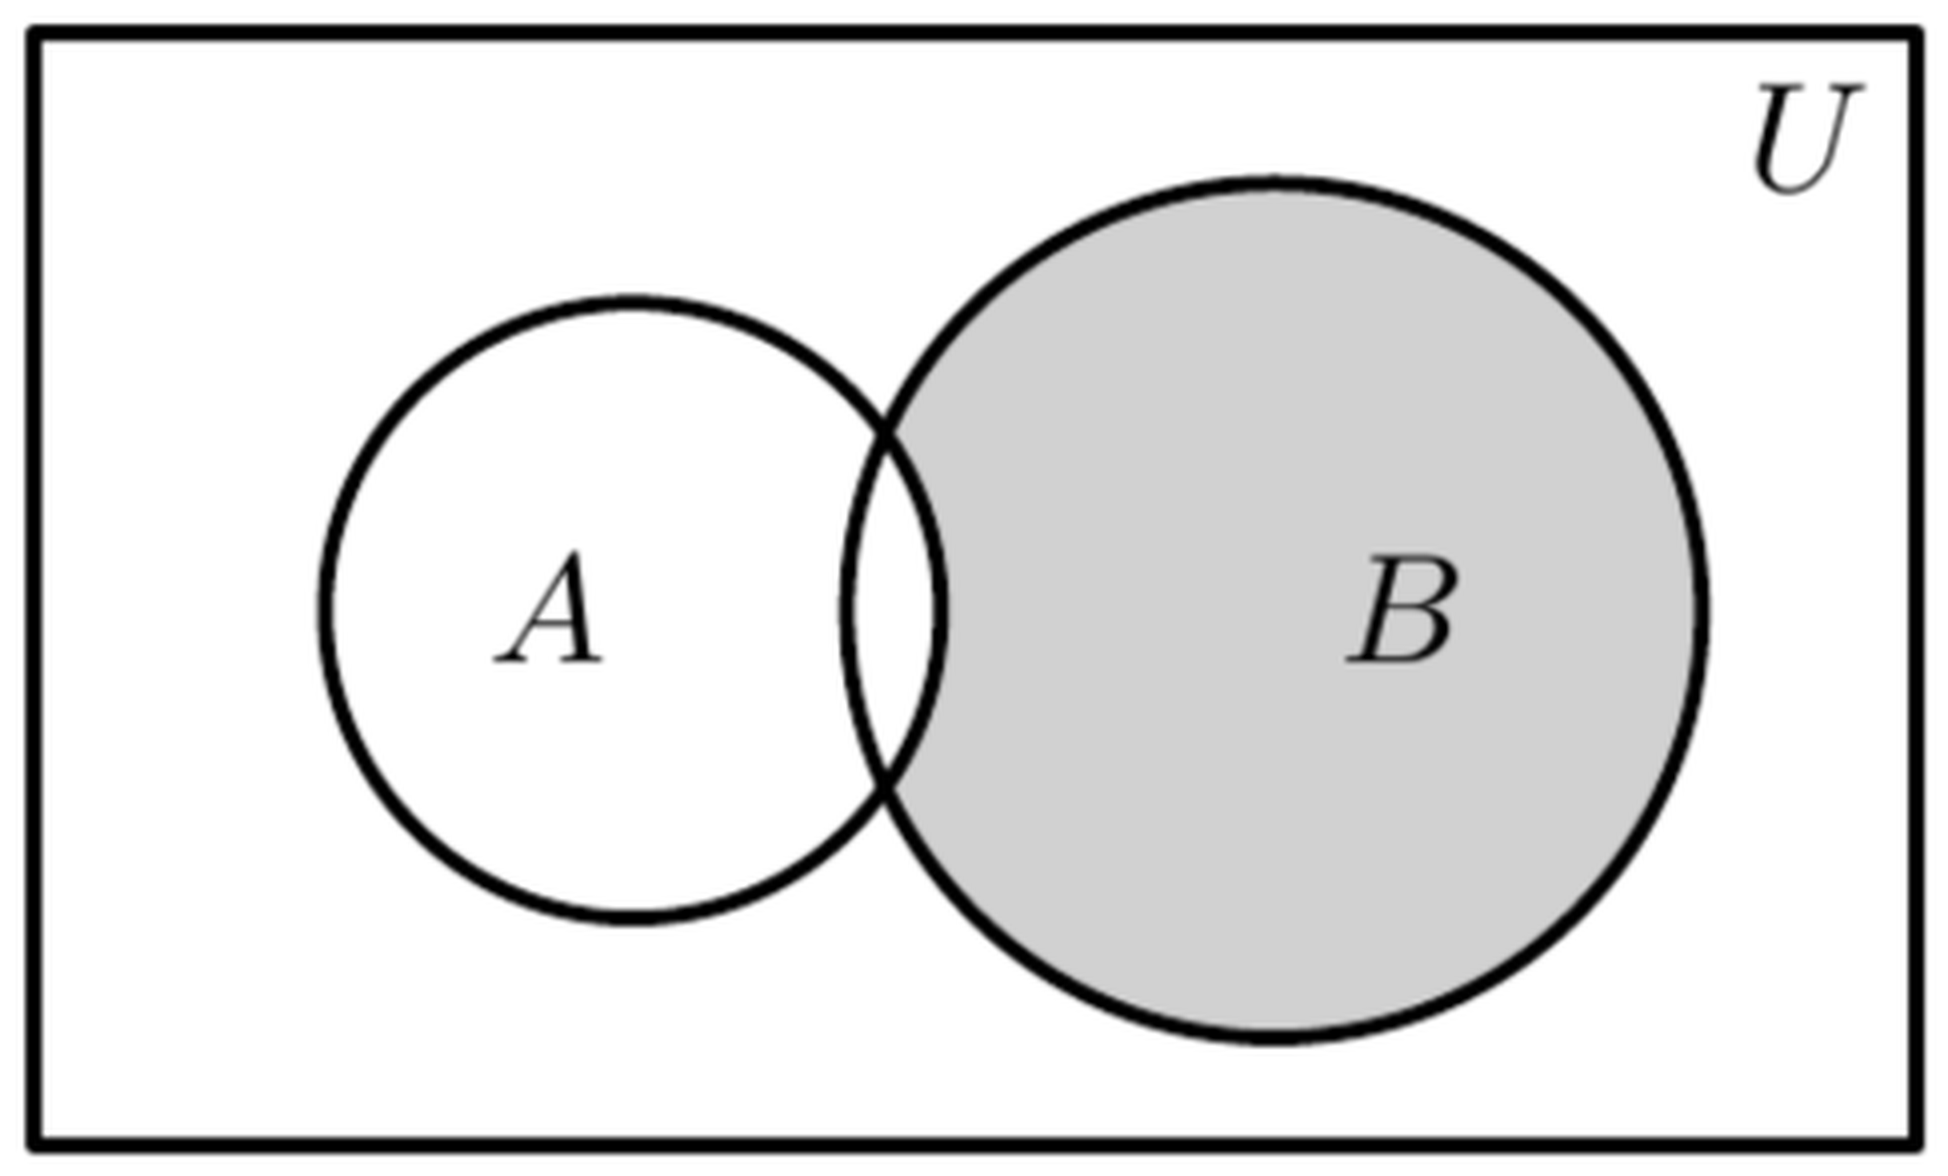
\includegraphics[width=0.38\textwidth]{figures/gao160_q4.png}
\end{center}

\ifanswer
\solbegin
\step{阴影部分表示 $B\cap\overline{A}=\{1,2\}$.}
\solend
\fi

% === Q5 === "图像"（有亻）照录；解析 1 行
\item 已知常数 $a>0$ 且 $a\ne1$，假设无论 $a$ 取何值，函数 $y=\log_a(5x-9)-4$ 的图像恒过一个定点，则这个定点的坐标为\blankline[4.4em].

\ifanswer
\solbegin
\step{$5x-9=1\Rightarrow x=2$，此时 $y=\log_a 1-4=-4$，定点为 $(2,-4)$.}
\solend
\fi

% === Q6 === 解析 2 行
\item 不等式 $(1-2x)^{\frac{3}{4}}>x^{\frac{3}{4}}$ 的解集为\blankline[4.4em].

\ifanswer
\solbegin
\step{定义域为 $\left[0,\dfrac{1}{2}\right]$，由幂函数的单调性，原不等式等价于 $1-2x>x$，}
\step{得 $0\leqslant x<\dfrac{1}{3}$，故解集为 $\left[0,\dfrac{1}{3}\right)$.}
\solend
\fi

% === Q7 === 绝对值 \lvert…\rvert；解析 2 行（跨 01—02 页）
\item 已知不等式 $\lvert x+3\rvert+\lvert x-2\rvert\geqslant 5$，当其等号成立时，$x$ 的取值范围是\blankline[4.4em].

\ifanswer
\solbegin
\step{$\lvert x+3\rvert+\lvert x-2\rvert=\lvert x+3\rvert+\lvert 2-x\rvert\geqslant\lvert(x+3)+(2-x)\rvert=5$，}
\step{等号成立当且仅当 $(x+3)(2-x)\geqslant0$，即 $x\in[-3,2]$.}
\solend
\fi

% === Q8 === 解析 4 行
\item 已知函数 $f(x)=\lvert\log_2 x\rvert$，若方程 $f(x)-t=0$ 有两个不同的实数根 $x_1,x_2$，则 $x_1+x_2$ 的取值范围是\blankline[4.4em].

\ifanswer
\solbegin
\step{方程有两个不同实根，必有 $t>0$，两根为 $2^t,2^{-t}$，}
\step{所以 $x_1+x_2=2^t+2^{-t}>2$（等号仅在 $t=0$ 时成立）.}
\step{任取 $s>2$，令 $a=\dfrac{s+\sqrt{s^2-4}}{2}>1$，取 $t=\log_2 a>0$，则 $x_1+x_2=a+\dfrac{1}{a}=s$，}
\step{所以取值范围为 $(2,+\infty)$.}
\solend
\fi

% === Q9 === 中文弯引号、\R、绝对值 \lvert…\rvert；解析 4 行
\item 已知 $a\in\R$，$b\in\R$，$p:\dfrac{1}{\lvert a\rvert}>\dfrac{1}{\lvert b\rvert}$，$q:\dfrac{1}{a}>\dfrac{1}{b}$，则 $p$ 是 $q$\blankline[4.4em]条件（用“充分非必要”、“必要非充分”、“充要”或“既非充分又非必要”填空）.

\ifanswer
\solbegin
\step{由 $p$、$q$ 中的分式有意义，$a\ne0$ 且 $b\ne0$.}
\step{当 $a=-1,b=-2$ 时，$p$ 成立而 $q$ 不成立，故 $p$ 不是 $q$ 的充分条件.}
\step{当 $a=1,b=-1$ 时，$q$ 成立而 $p$ 不成立，故 $p$ 不是 $q$ 的必要条件.}
\step{故 $p$ 是 $q$ 的充分非必要条件.}
\solend
\fi

% === Q10 === 解析 3 行；其后独立【注】按语 5 行（见头注 ② ⑯、⑤ 1）
\item 已知常数 $a>0$，函数 $y=\dfrac{2^x}{2^x+ax}$ 的图像经过点 $P\left(p,\dfrac{5}{6}\right)$、$Q\left(q,\dfrac{1}{6}\right)$，若 $2^{p+q}=3pq$，则 $a=$\blankline[4.4em].

\ifanswer
\solbegin
\step{由 $\dfrac{2^p}{2^p+ap}=\dfrac{5}{6}$ 得 $2^p=5ap$；由 $\dfrac{2^q}{2^q+aq}=\dfrac{1}{6}$ 得 $2^q=\dfrac{aq}{5}$.}
\step{$2^p>0$，$2^q>0$，$a>0$，得 $p>0$，$q>0$.}
\step{两式相乘得 $2^{p+q}=a^2pq$，又 $2^{p+q}=3pq$ 且 $pq\ne0$，故 $a^2=3$，$a=\sqrt{3}$.}
\solend
% 【注】按语（讲评版编者按，5 个印刷行，仅答案版出，不属于任何题的【解析】）
\stepm{【注】}{按原卷数据严格推敲，点 $Q$ 其实不存在：$a=\sqrt{3}$ 时 $2^q=\dfrac{\sqrt{3}}{5}q<q$；而当 $q>0$}
\step{时，取非负整数 $n$ 使 $n\leqslant q<n+1$，由 $2^{k+1}=2^k+2^k\geqslant2^k+1$ 逐次推得 $2^n\geqslant n+1$，于是}
\step{$2^q\geqslant2^n\geqslant n+1>q$，矛盾. 所以题设条件互相矛盾，严格说本题无解；$\sqrt{3}$ 是由题给关}
\step{系直接推出的值，按命题意图作为答案. 原卷数据疑似有误（同型常见题为 $P\left(p,\dfrac{6}{5}\right)$、}
\step{$Q\left(q,-\dfrac{1}{5}\right)$、$2^{p+q}=36pq$，得 $a=6$）.}% 见头注 ⑤ 1，照录未改
\fi

% === Q11 === 纳皮尔对数材料题；\Z、大数；解析 6 行
\item 17 世纪初，约翰·纳皮尔为了简化计算而发明了对数. 对数的发明是数学史上的重大事件，恩格斯曾经把笛卡尔的坐标系、纳皮尔的对数、牛顿和莱布尼兹的微积分共同称为 17 世纪的三大数学发明. 我们知道，任何一个正实数 $N$ 可以表示成 $N=a\times10^n$ ($1\leqslant a<10,n\in\Z$) 的形式，这便是科学记数法，若两边取常用对数，有 $\lg N=n+\lg a$，则可以估计 $3^{2026}$ 的最高位上的数值为\blankline[4.4em].

\ifanswer
\solbegin
\step{设 $3^{2026}=a\times10^n$ ($1\leqslant a<10,n\in\Z$)，则 $2026\lg 3=n+\lg a$.}
\step{用 $\lg 3\approx 0.4771$ 粗估，得 $2026\lg 3\approx 966.60$.}
\step{为核验误差，用 $0.47712<\lg 3<0.47713$，}
\step{得 $966.64512<2026\lg 3<966.66538$，因此 $n=966$.}
\step{于是 $\lg 4\approx 0.60206<0.64512<\lg a<0.66538<\lg 5\approx 0.69897$，}
\step{所以 $4<a<5$，最高位为 4，估算误差不影响结论.}
\solend
\fi

% === Q12 === 自定义"性质 P"；文本圈数字①②③；解析 19 行（跨 03—05 页）
\item 对于数集 $X=\{-1,x_1,x_2,x_3,\cdots,x_n\}$，其中 $0<x_1<x_2<x_3<\cdots<x_n$，$n\geqslant2$，定义点集 $Y=\{(s,t)\mid s\in X,t\in X\}$，若对于任意 $(s_1,t_1)\in Y$，存在 $(s_2,t_2)\in Y$，使得 $s_1s_2+t_1t_2=0$，则称集合 $X$ 具有性质 $P$. 则下列命题中为真命题的是\blankline[4.4em].

① $X=\{-1,1,2\}$ 具有性质 $P$；②若集合 $X$ 具有性质 $P$，则 $1\in X$；

③集合 $X$ 具有性质 $P$，若 $x_1=\dfrac{1}{2}$，则 $x_n=2$.

\ifanswer
\solbegin
\step{因为 $X=\{-1,1,2\}$，}
\step{所以 $Y=\{(-1,-1),(1,1),(2,2),(-1,1),(-1,2),(1,-1),(1,2),(2,-1),(2,1)\}$，}
\step{由集合 $X$ 具有性质 $P$ 的定义，对于任意 $(s,t)\in Y$，}
\step{若 $s>0$，$t>0$，则 $s=t$ 或 $(s,t)=(1,2)$ 或 $(s,t)=(2,1)$，}
\step{若 $s=t$，取 $s_2=-1$，$t_2=-1$，则 $ss_2+tt_2=0$；}
\step{若 $(s,t)=(1,2)$，取 $s_2=2$，$t_2=-1$，则 $ss_2+tt_2=0$；}
\step{若 $(s,t)=(2,1)$，取 $s_2=-1$，$t_2=2$，则 $ss_2+tt_2=0$；}
\step{若 $s$、$t$ 有一个为负数，则 $s=-1$ 或 $t=-1$，}
\step{若 $s=-1$，则取 $s_2=t$，$t_2=1$，则 $ss_2+tt_2=0$；}
\step{若 $t=-1$，则取 $s_2=1$，$t_2=s$，则 $ss_2+tt_2=0$；故①正确；}
\step{对于任意 $(s_1,t_1)\in Y$，存在 $(s_2,t_2)\in Y$，使得 $s_1s_2+t_1t_2=0$，}
\step{取 $(x_1,x_1)\in Y$，存在 $(x_p,x_q)$ 使得 $x_1x_p+x_1x_q=0$，所以 $x_p+x_q=0$，}
\step{不妨设 $x_p=1$，$x_q=-1$，所以若集合 $X$ 具有性质 $P$，则 $1\in X$，故②正确；}
\step{③假设 $x_n>1$，令 $s_1=\dfrac{1}{2},t_1=x_n$，则存在 $s$、$t\in X$ 使得 $\dfrac{1}{2}s+tx_n=0$，}
\step{同②得 $s$、$t$ 中必有一个数为 $-1$，}
\step{若 $s=-1$，则 $tx_n=\dfrac{1}{2}$，于是 $t=\dfrac{1}{2x_n}<\dfrac{1}{2}=x_1$，矛盾，}
\step{若 $t=-1$，则 $\dfrac{1}{2}s=x_n\cdot(-1)$，于是 $s=2x_n>x_n$，也矛盾，}% 原卷如此（与结论符号不自洽），照录未改，见头注 ⑤ 2
\step{所以 $x_n\leqslant1$，又由②得 $1\in X$，所以 $x_n\geqslant1$，所以 $x_n=1$，故③错误，}
\step{故真命题是①②.}
\solend
\fi

\end{enumerate}

% 答案版里填空解析把页排满，节标题会落到页末、与第 13 题分家（切页审计 B 类）；
% 守卫放 \bigsec 之前，连节标题一起量页高（高一157 成例）
\needvspace{7cm}
\bigsec{二、选择题}

\begin{enumerate}
\setcounter{enumi}{12}

% === Q13 === "图像"照录；解析 1 行，故选 $B$
\item 下列函数中，图像与函数 $y=3^x$ 图像关于 $y$ 轴对称的是\mbox{（\quad）}

\keepwithprev
A. $y=x^3$\qquad B. $y=\left(\dfrac{1}{3}\right)^x$\qquad C. $y=-3^x$\qquad D. $y=\log_3 x$

\ifanswer
\solbegin
\step{将 $x$ 换为 $-x$，得对称图像对应的函数为 $y=3^{-x}=\left(\dfrac{1}{3}\right)^x$，故选 $B$.}
\solend
\fi

% === Q14 === 中文弯引号；解析 2 行（跨 05 页上下），故选 $B$
\item 命题“存在 $x\in(1,+\infty)$，使得 $f(x)>0$”的否定形式为\mbox{（\quad）}

\keepwithprev
A. 不存在 $x\in(-\infty,1]$，使得 $f(x)>0$\qquad B. 对任意 $x\in(1,+\infty)$，有 $f(x)\leqslant0$

C. 对任意 $x\in(-\infty,1]$，有 $f(x)\leqslant0$\qquad D. 存在 $x\in(1,+\infty)$，使得 $f(x)\leqslant0$

\ifanswer
\solbegin
\step{将“存在”改为“对任意”，$x$ 的范围不变，并将 $f(x)>0$ 否定为 $f(x)\leqslant0$，}
\step{故选 $B$.}
\solend
\fi

% === Q15 === \R；四选项两行；解析 3 行，故选 $D$
\item 设 $a>0$，$s\in\R$. 下列各项中，能推出 $a^s>a$ 的一项是\mbox{（\quad）}

\keepwithprev
A. $a>1$，且 $s>0$\qquad B. $a>1$，且 $s<0$

C. $0<a<1$，且 $s>0$\qquad D. $0<a<1$，且 $s<0$

\ifanswer
\solbegin
\step{当 $a>1$ 时，$a^s>a\Leftrightarrow s>1$，A、B 均不能保证.}
\step{当 $0<a<1$ 时，$a^s>a\Leftrightarrow s<1$，C 不能保证，D 中 $s<0<1$，满足要求；}
\step{故选 $D$.}
\solend
\fi

% === Q16 === 题目配图（三版都出）；几何符号 \triangle ABC；解析 3 行，故选 $C$
\needvspace{8cm}
\item 数学说明的方法多种多样，其中利用图形说明就是一种重要方法. 如图所示，在等腰直角三角形 $\triangle ABC$ 中，点 $O$ 为斜边 $AB$ 的中点，点 $D$ 为斜边 $AB$ 上异于顶点的一个动点，设 $AD=a$，$BD=b$，则可用该图形能说明的不等式为\mbox{（\quad）}

\begin{center}
% Q16 等腰直角三角形 ABC 图（C/A/O/D/B 标注）取 05 页右下，去粉色水印、去色、3× LANCZOS 放大；三版都出
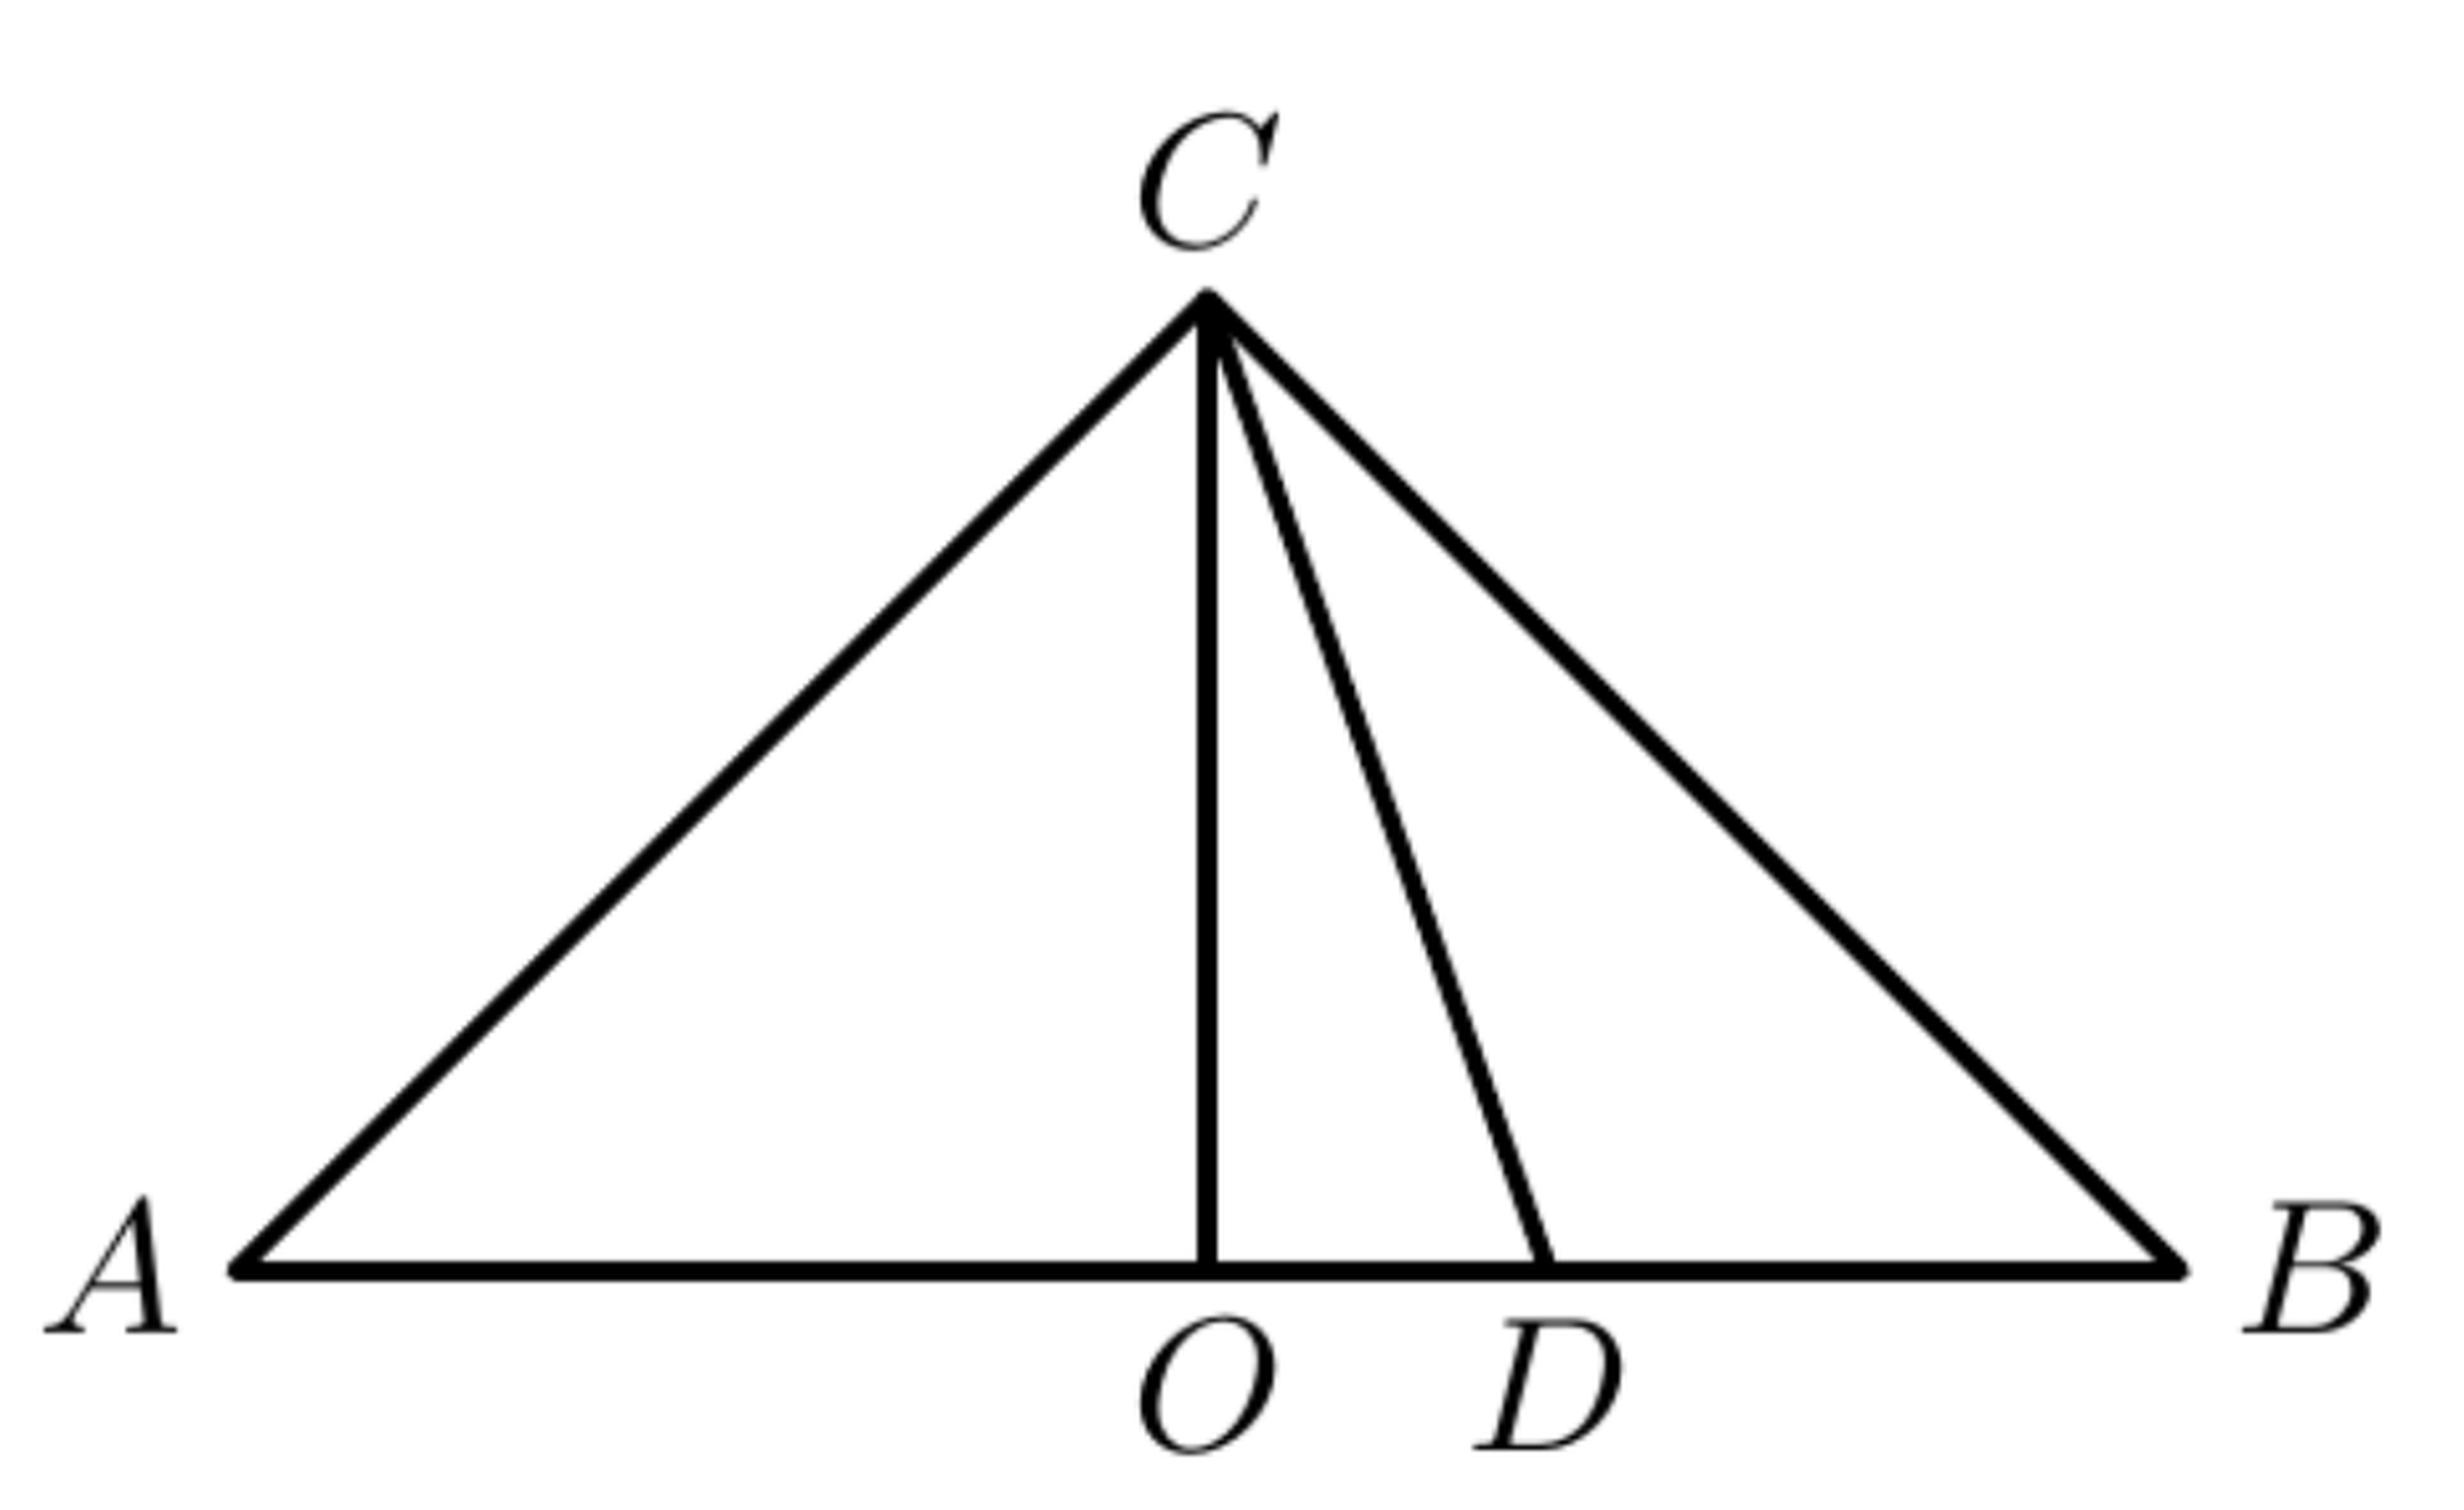
\includegraphics[width=0.34\textwidth]{figures/gao160_q16.png}
\end{center}

\keepwithprev
A. $\dfrac{a+b}{2}\geqslant\sqrt{ab}$ ($a>0,b>0$)\qquad B. $a^2+b^2\geqslant2\sqrt{ab}$ ($a>0,b>0$)

C. $\dfrac{a+b}{2}\leqslant\sqrt{\dfrac{a^2+b^2}{2}}$ ($a>0,b>0$)\qquad D. $\dfrac{2ab}{a+b}\leqslant\sqrt{ab}$ ($a>0,b>0$)

\ifanswer
\solbegin
\step{$CO=AO=\dfrac{a+b}{2},OD=\left\lvert a-\dfrac{a+b}{2}\right\rvert=\dfrac{\lvert a-b\rvert}{2}$，}
\step{$CD=\sqrt{CO^2+OD^2}=\sqrt{\dfrac{a^2+b^2}{2}}\geqslant CO=\dfrac{a+b}{2}$，}
\step{等号当且仅当 $a=b$ 时成立，故选 $C$.}
\solend
\fi

\end{enumerate}

\bigsec{三、解答题}

\begin{enumerate}
\setcounter{enumi}{16}

% === Q17 === cases 块算一行；判别式印等腰偏高三角 \Delta；解析 7 行
\item 已知幂函数 $f(x)=(m^2-2m-2)x^{m-1}$ 在 $(0,+\infty)$ 上是严格增函数.

(1) 求 $m$ 的值；

(2) 若关于 $x$ 的方程 $f(x)=(t+1)x-t^2$ 有两个不相等的正实根，求实数 $t$ 的取值范围.

\ifanswer
\solbegin
\step{(1) 幂函数的系数为 1，因此 $m^2-2m-2=1\Leftrightarrow(m-3)(m+1)=0$，}
\step{解得 $m=3$ 或 $m=-1$.}
\step{由 $f(x)$ 在 $(0,+\infty)$ 上严格递增，得 $m-1>0$，所以 $m=3$，}
\step{此时 $f(x)=x^2$.}
\step{(2) 原方程化为 $x^2-(t+1)x+t^2=0$，}
\step{方程有两个不相等的正实根，则 $\begin{cases}\Delta=(t+1)^2-4t^2=(1-t)(3t+1)>0\\t+1>0\\t^2>0\end{cases}$，}% 判别式原卷印等腰偏高三角 \Delta，照录
\step{得 $t\in\left(-\dfrac{1}{3},0\right)\cup(0,1)$.}
\solend
\fi

% === Q18 === 补集上划线 \overline{A}、\subseteq 带下划线、\varnothing；解析 8 行
\item 已知集合 $A=\{x\mid\lvert x-a\rvert<a-3\}$，$B=\left\{x\mid\dfrac{x+1}{x-2}\geqslant2\right\}$.

(1) 若 $a=5$，求 $\overline{A}\cap B$；

(2) 若 $A\cap B=A$，求实数 $a$ 的取值范围.

\ifanswer
\solbegin
\step{(1) $\dfrac{x+1}{x-2}\geqslant2\Leftrightarrow\dfrac{5-x}{x-2}\geqslant0\Leftrightarrow2<x\leqslant5,B=(2,5]$，}
\step{当 $a=5$ 时，$A=\{x\mid\lvert x-5\rvert<2\}=(3,7)$，于是 $\overline{A}=(-\infty,3]\cup[7,+\infty)$，}
\step{因此 $\overline{A}\cap B=(2,3]$.}
\step{(2) $A\cap B=A$ 等价于 $A\subseteq B$.}
\step{当 $a\leqslant3$ 时，$a-3\leqslant0$，$A=\varnothing$，满足条件.}
\step{当 $a>3$ 时，$\lvert x-a\rvert<a-3\Leftrightarrow3<x<2a-3,A=(3,2a-3)$，}
\step{此时 $A\subseteq B=(2,5]$ 等价于 $2a-3\leqslant5$，即 $a\leqslant4$，结合 $a>3$ 得 $3<a\leqslant4$.}
\step{合并两种情形，实数 $a$ 的取值范围为 $(-\infty,4]$.}
\solend
\fi

% === Q19 === 数据表 tabular 重排（高一130 成例）；cases 块算一行；解析 6 行
\item 作为我国最高水平的综合性运动会，全运会汇聚了国内顶尖体育健儿，某代表队从第 8 届全运会开始登上赛场，且参赛运动员人数逐年递增. 设 $t$ 为该代表队参赛后经过的届数，即第 8 届为 $t=0$，第 9 届为 $t=1$，以此类推. 经过 $t$ 届，运动员人数为 $y$ 人，具体数据如下：

\begin{center}
\begin{tabular}{cccccc}
$t$ & 0 & 1 & 2 & 3 & 4 \\
\hline
届数 & 8 & 9 & 10 & 11 & 12 \\
运动员人数（$y$ 人） & 4 & 11 & 25 & 53 & 109
\end{tabular}
\end{center}

(1) 现有以下两种函数模型：① $y=a\cdot b^t+c$ ($a>0,b>1$)；② $y=\log_a(t+b)+c$ ($b>0,a>1$). 请根据上表中运动员人数的增长规律，选出你认为符合的函数模型（不用说明理由），并利用表中前 3 组数据求出相应的函数解析式；

(2) 若参赛运动员人数按照 (1) 中求得的模型继续增长，在第几届全运会时，该代表队运动员人数将会首次超过 1000 人？

\ifanswer
\solbegin
\step{(1) 选模型①，将前 3 组数据代入，得 $\begin{cases}a+c=4\\ab+c=11\\ab^2+c=25\end{cases}$，}% 原卷印"选模型①"（圈数字①），OCR 误作"四"，照录①，见头注 ⑤ 3
\step{相邻两式相减，得 $a(b-1)=7$，$ab(b-1)=14$，}
\step{两式相除得 $b=2$，进而 $a=7$，$c=-3$，所求函数解析式为 $y=7\cdot2^t-3$.}
\step{(2) $y=7\cdot2^t-3$ 随 $t$ 的增大而增大，且 $t=7$ 时，$y=893<1000$；}
\step{$t=8$ 时，$y=1789>1000$，}
\step{$t$ 为非负整数，首次超过 1000 人时 $t=8$，对应第 $8+8=16$ 届全运会.}
\solend
\fi

% === Q20 === 解析 12 行（跨 08—09 页）
\item 已知函数 $f(x)=\log_a(a-a^x)$.

(1) 求该函数的定义域；

(2) 若 $a>1$，试判断关于 $x$ 的方程 $f(x)=2$ 是否有实数解，并说明理由；

(3) 若当 $x\in(-\infty,0]$ 时，关于 $x$ 的不等式 $f(x)\geqslant-1$ 恒成立，求实数 $a$ 的取值范围.

\ifanswer
\solbegin
\step{(1) 对数的底数须满足 $a>0$ 且 $a\ne1$，真数须满足 $a-a^x>0$，即 $a^x<a^1$.}% 原卷印 $a^1$，照录未化简，见头注 ⑤ 4
\step{当 $a>1$ 时，$x<1$，定义域为 $(-\infty,1)$.}
\step{当 $0<a<1$ 时，$x>1$，定义域为 $(1,+\infty)$.}
\step{(2) 当 $a>1$ 时，若 $f(x)=2$，则 $a-a^x=a^2\Rightarrow a^x=a(1-a)<0$，}
\step{这与 $a^x>0$ 矛盾，因此方程无实数解.}
\step{(3) 不等式在 $(-\infty,0]$ 上恒成立，须先保证该区间包含于函数的定义域，}
\step{由 (1) 得 $a>1$.}
\step{当 $x\leqslant0$ 时，$0<a^x\leqslant1$，所以 $a-a^x\geqslant a-1>0$.}
\step{由对数函数的单调性，$f(x)=\log_a(a-a^x)\geqslant\log_a(a-1)=f(0)$，}
\step{等号当且仅当 $x=0$ 时成立，}
\step{因此所求条件等价于 $\log_a(a-1)\geqslant-1\Leftrightarrow a-1\geqslant\dfrac{1}{a}\Leftrightarrow a^2-a-1\geqslant0$，}
\step{结合 $a>1$，得 $a\in\left[\dfrac{1+\sqrt{5}}{2},+\infty\right)$.}
\solend
\fi

% === Q21 === "和积平衡集"定义证明题；\N；解析 18 行（跨 09—10 页）
\item 已知有限集 $A=\{a_1,a_2,\cdots,a_n\}$ ($n\geqslant2,n\in\N$)，如果 $A$ 中元素 $a_i$ ($i=1,2,3,\cdots,n$) 满足 $a_1+a_2+a_3+\cdots+a_n=a_1\times a_2\times\cdots\times a_n$，就称 $A$ 为“和积平衡集”.

(1) 分别判断集合 $A=\{1,2,3,4\}$，$B=\{4+2\sqrt{2},4-2\sqrt{2}\}$ 是否为“和积平衡集”；

(2) 已知 $a_1$、$a_2$ 是两个不同的正数，且 $\{a_1,a_2\}$ 是“和积平衡集”，请用反证法证明：$a_1$、$a_2$ 至少有一个大于 2；

(3) 若 $a_i\geqslant1$，且 $a_i\in\N$，求所有符合条件的“和积平衡集”.

\ifanswer
\solbegin
\step{(1) 因为 $1+2+3+4=10\ne24=1\times2\times3\times4$，所以 $A$ 不是“和积平衡集”.}
\step{因为 $(4+2\sqrt{2})+(4-2\sqrt{2})=8=(4+2\sqrt{2})(4-2\sqrt{2})$，}
\step{所以 $B$ 是“和积平衡集”.}
\step{(2) 假设 $a_1$、$a_2$ 都不大于 2，则 $\dfrac{1}{a_1}\geqslant\dfrac{1}{2},\dfrac{1}{a_2}\geqslant\dfrac{1}{2}$，}
\step{由于 $a_1\ne a_2$，上述两个不等式至少有一个严格成立.}
\step{而 $a_1+a_2=a_1a_2$，两边除以 $a_1a_2>0$，得 $1=\dfrac{1}{a_1}+\dfrac{1}{a_2}>\dfrac{1}{2}+\dfrac{1}{2}=1$，矛盾，}
\step{所以 $a_1$、$a_2$ 至少有一个大于 2.}
\step{(3) 不妨设 $a_1<a_2<\cdots<a_n$，由各元素均为正整数，得 $a_i\geqslant i$.}
\step{若 $n\geqslant4$，因其余因子均不小于 1，}
\step{有 $a_1a_2\cdots a_n\geqslant a_2a_{n-1}a_n\geqslant2(n-1)a_n>na_n>a_1+a_2+\cdots+a_n$，}
\step{与和积平衡条件矛盾，因此只需讨论 $n=2,3$.}
\step{当 $n=2$ 时，$a_1+a_2=a_1a_2\Leftrightarrow(a_1-1)(a_2-1)=1$，}
\step{两个因子均为非负整数，只能有 $a_1=a_2=2$，与元素互不相同矛盾.}
\step{当 $n=3$ 时，若 $a_1\geqslant2$，则 $a_2\geqslant3$，从而 $a_1a_2a_3\geqslant6a_3>3a_3>a_1+a_2+a_3$，}
\step{矛盾，因此 $a_1=1$.}
\step{此时 $1+a_2+a_3=a_2a_3\Leftrightarrow(a_2-1)(a_3-1)=2$，}
\step{由 $1\leqslant a_2-1<a_3-1$，得 $a_2-1=1$、$a_3-1=2$，即 $a_2=2$、$a_3=3$.}
\step{检验 $1+2+3=1\times2\times3=6$，所求集合为 $\{1,2,3\}$.}
\solend
\fi

\end{enumerate}

\end{document}
"
% 紧凑版：xelatex "\def\iscompact{1}% 高一160_奉贤中学_期中.tex
%   —— 高一上数学"2026-2027 年奉贤中学高一上期中"（试卷版/答案版/紧凑版）
% 试卷版：xelatex 高一160_奉贤中学_期中.tex
% 答案版：xelatex "\def\isanswer{1}% 高一160_奉贤中学_期中.tex
%   —— 高一上数学"2026-2027 年奉贤中学高一上期中"（试卷版/答案版/紧凑版）
% 试卷版：xelatex 高一160_奉贤中学_期中.tex
% 答案版：xelatex "\def\isanswer{1}\input{高一160_奉贤中学_期中.tex}"
% 紧凑版：xelatex "\def\iscompact{1}\input{高一160_奉贤中学_期中.tex}"
%
% ① 原始材料：微信公众号"魔都数学加油站"文章，连载"27学年高一160"，原卷卷面标题
% "2026-2027 年奉贤中学高一上期中"（卷面未印副标题、未印连载号）。
% 正文为 10 张 PNG 页（01/04/10 为 2560×3620，02/03/05/06/07/08/09 为
% 4762×6735，同一篇各页分辨率混排，逐页按各自分辨率裁图核对）。
% 体例：讲评版——填空 3—12（10 题）、选择 13—16（4 题）、解答 17—21（5 题），
% 共 19 题，自第 3 题起编（1、2 未印在本篇）；19 题逐题印【解析】，无只印【答案】
% 的题；四道选择题答案在解析末句"故选 $B$/$B$/$D$/$C$"，题干括号
% \mbox{（\quad）} 留空、不另提 \ans{}。题目、答案、解析均据原图转录；卷面粉红色
% 水印"魔都数学加油站"及公众号页脚未录入。
% 全卷插图清单（逐页通读 10 页确认）：2 幅，均为题目配图、三版都出——
%   · Q4 韦恩图（01 页右侧：矩形全集 U、两圆 A/B、阴影部分 B∩上划线 A、
%     标注 U/A/B），裁 figures/gao160_q4.png；
%   · Q16 等腰直角三角形 ABC 图（05 页右下：C 顶点、A/O/D/B 共线底边、
%     CO 与 CD 两条线段），裁 figures/gao160_q16.png；
%   两图均取原卷截图 3—4× LANCZOS 放大、去粉色水印、转灰度、autocontrast；
%   Q4 图左侧题干残字"示"、Q16 图左侧题干残字均已裁白。
%   Q19 有一张 3 行数据表（t／届数／运动员人数（y 人），t=0..4），按全稿
%   成例（高一130）用 tabular 重排，不做成 png；其余各页无题目配图、
%   无解析内配图、无其它表格、无"如图"处。
%
% 卷首标题：原卷印作"2026-2027 年奉贤中学高一上期中"，年份区间按全稿惯例排 en dash；
% 原卷卷面未印副标题，本稿按同期中卷知识模块口径补出"集合与常用逻辑用语、不等式、函数"。
%
% ② 与原卷的排版差异／照录项清单：
%   ① 原文从第 3 题起，本稿保留原题号；共 19 题三节，解答题 5 题到 21；
%      三节各自一个 enumerate + \setcounter{enumi}{2}/{12}/{16}（不贯穿），
%      用 \examtitlest[3] 起手；
%   ② 混合体例说明：19 题全印【解析】、用 \solbegin…\solend，无只印【答案】
%      或答案印括号内的题；四道选择题答案在解析末句"故选 $B$/$B$/$D$/$C$"
%      （逐个放大复核）、括号 \mbox{（\quad）} 留空、不另提 \ans{}；答案版
%      【答案】/【解析】标记数 = 19 = 全卷题数（0 个 \ans ＋ 19 个 \solbegin）；
%   ③ 原卷卷面未印副标题，本稿按知识模块口径补出；
%   ④ 原卷填空横线按全稿惯例排 \blankline[4.4em]；选择题括号排 \mbox{（\quad）}、
%      四道选择题的选项段前按惯例各加 \keepwithprev；解答题不留作答区、不加
%      \anspace（原卷为讲评版，109—113 起全稿不用 \anspace）；
%   ⑤ 数集归一：Q4"$U=\Z$"、Q9"$a\in\R$，$b\in\R$"、Q11"$n\in\Z$"、
%      Q15"$s\in\R$"、Q21"$n\in\N$""$a_i\in\N$"原卷印正体粗体 Z/R/N，
%      按全稿惯例归一 \Z／\R／\N；集合描述竖线排 \mid（Q3、Q4、Q12、
%      Q18、Q21）；空集 \varnothing（Q18 解析 (2)）；补集照原卷上划线排
%      \overline{A}（Q4 解析、Q18 (1) 题干与解析）；子集符号 Q18 两处
%      "$A\subseteq B$"印带下划线 ⊆、照录 \subseteq；
%   ⑥ 绝对值排 \lvert…\rvert（Q7、Q8 题干与解析、Q9 题干、Q16 解析、
%      Q18 题干与解析），Q16 解析的 \left\lvert…\right\rvert 与 \lvert…\rvert
%      均在同一 $…$ 组内配对平衡；
%   ⑦ 判别式两形混用逐处照录不统一（放大逐处确认）：Q3 解析
%      "$\triangle=1^2-4a\times\frac{1}{4}=0$"原卷印扁等边三角、照录
%      \triangle；Q17 解析 cases 块"$\Delta=(t+1)^2-4t^2=(1-t)(3t+1)>0$"
%      原卷印等腰偏高三角、照录 \Delta；Q16 题干几何符号"$\triangle ABC$"
%      按全稿几何三角形记号惯例归一 \triangle（参照 高一150／132 成例）；
%   ⑧ 不等号按全稿惯例排 \leqslant／\geqslant；中文弯引号照录：Q9 题干
%      "充分非必要""必要非充分""充要""既非充分又非必要"、Q14 题干
%      "存在 $x\in(1,+\infty)$，使得 $f(x)>0$"与解析"存在""对任意"、
%      Q21 题干与解析多处"和积平衡集"；注释里一律 ASCII 引号；
%   ⑨ 文本圈数字逐处照录：Q12 题干①②③、Q12 解析"故①正确""同②得"
%      "故②正确""③假设""故③错误""故真命题是①②"、Q19 题干①②与解析
%      "选模型①"，均为印刷圈数字（非 \textcircled、非数学模式）；
%   ⑩ 半角逗号在数学组之间是全稿惯例、非笔误，逐处照录（Q8"$2^t,2^{-t}$"、
%      Q9"$a=-1,b=-2$""$a=1,b=-1$"、Q11"$1\leqslant a<10,n\in\Z$"、
%      Q12"$s_1=\frac{1}{2},t_1=x_n$"、Q16 选项"$a>0,b>0$"与解析
%      "$CO=AO=\frac{a+b}{2},OD=...$"、Q18"$2<x\leqslant5,B=(2,5]$"
%      "$3<x<2a-3,A=(3,2a-3)$"、Q21"$n=2,3$"等）；行中全角逗号／顿号
%      照录（Q15 选项"$a>1$，且 $s>0$"、Q12 解析"$s$、$t$"、Q21 解析
%      "$a_1$、$a_2$"），顿号一律移出数学模式；
%   ⑪ "图像／图象"逐处照录：本卷 Q5"的图像恒过一个定点"、Q10"的图像经过点"、
%      Q13 题干两处"图像"与解析"对称图像对应的函数"均印"图像"（有亻）；
%      Q16 印"图形"（利用图形说明、该图形能说明），无"图象"用例；
%   ⑫ 复杂式照录别简化：Q3 $ax^2+x+\frac14=0$、Q5 $y=\log_a(5x-9)-4$、
%      Q6 $(1-2x)^{\frac34}>x^{\frac34}$ 与 $\left[0,\frac12\right]$、
%      Q8 $\frac{s+\sqrt{s^2-4}}{2}$、Q10 $y=\frac{2^x}{2^x+ax}$ 与
%      $\frac{2^p}{2^p+ap}=\frac56$、$\frac{2^q}{2^q+aq}=\frac16$、
%      Q11 $N=a\times10^n$ 与 $3^{2026}$、$2026\lg3\approx966.60$、
%      $966.64512<2026\lg3<966.66538$、Q12 $Y=\{(s,t)\mid s\in X,t\in X\}$
%      与 $\frac12 s+tx_n=0$、Q16 $\sqrt{\frac{a^2+b^2}{2}}$、
%      Q17 $x^2-(t+1)x+t^2=0$ 与 $\left(-\frac13,0\right)\cup(0,1)$、
%      Q18 $\frac{5-x}{x-2}\geqslant0$、Q19 $y=a\cdot b^t+c$ 与
%      $y=\log_a(t+b)+c$、$y=7\cdot2^t-3$、Q20 $f(x)=\log_a(a-a^x)$
%      与 $a^2-a-1\geqslant0$、$\left[\frac{1+\sqrt5}{2},+\infty\right)$、
%      Q21 $4+2\sqrt2$ 与 $(a_2-1)(a_3-1)=2$ 等；
%   ⑬ 子题标号 (1)(2)(3) 按全稿惯例排半角括号；行末／行中句点按全稿惯例
%      排 ASCII `.`（不是全角「．」）；cases 块整体算一个印刷行
%      （Q17 解析、Q19 解析 (1)）；
%   ⑭ 配图：Q4／Q16 题目配图（三版都出）放 \item 内题干之后 \begin{center}，
%      各用 \needvspace{8cm} 守卫把整块推走，**守卫放在 \item 之前**
%      （见 高一153 Q11/Q19 成例与切页审计 B 类坑）；
%   ⑮ 一条 \step = 原卷解析的一个印刷行；跨上下半页的重叠行只算一次
%      （Q4 解析、Q9 解析首行、Q11 解析首行、Q12 解析"若 $s=-1$…"一行、
%      Q18 解析"此时 $A\subseteq B=(2,5]$…"一行、Q20 (2) 题干、
%      Q21 解析"由 $1\leqslant a_2-1<a_3-1$…"一行）；原卷折行别合并；
%   ⑯ Q10 之后另有一整块【注】按语（03 页上半，5 个印刷行），是讲评版作者对
%      原卷数据自相矛盾的加注、不属于任何题的【解析】。本稿按 高一53
%      "注：…"成例放 Q10 的 \solend 之后、Q10 的 \fi 收尾之前：
%      **整块只保留 Q10 那一层外层 \ifanswer**（那个 \fi 就是 Q10 的收尾），
%      块内 \stepm{【注】}{首行} ＋ 4 条 \step 各自自带内层 \ifanswer…\fi
%      （\step／\stepm 宏内自带，源码里不手动再包一层 \ifanswer，
%      否则 题目溯源.py 的 strip_answers 非贪婪正则会错切）；
%      \stepm 第一参数直接用「【注】」作标签，与全稿 \ans 的【答案】、
%      \solbegin 的【解析】同性质，未加粗以外不另加任何样式；
%      5 行仅答案版出、不新增 \item、不影响溯源，头注 ③ 单列登记、
%      不计入 19 题逐题 \step 账；\stepm 把【注】排成加粗着色标签
%      （原卷为黑色加粗），此一处着色差异在此登记；
%   ⑰ 原卷用字照录：Q11"约翰·纳皮尔""莱布尼兹"（原卷作"兹"，非通行"茨"）、
%      "17 世纪的三大数学发明"；Q16"数学说明的方法""点 $D$ 为斜边 $AB$ 上
%      异于顶点的一个动点"；Q19"登上赛场""以此类推"；
%
% ③ 行数复核：一条 \step = 原卷解析的一个印刷行，cases 块作一个印刷行计。
%   逐题数（逐页核对定稿）：Q3：5；Q4：1；Q5：1；Q6：2；Q7：2；Q8：4；
%   Q9：4；Q10：3；Q11：6；Q12：19；Q13：1；Q14：2；Q15：3；Q16：3；
%   Q17：7；Q18：8；Q19：6；Q20：12；Q21：18。
%   合计 107 条 \step（19 题逐题印刷行账），与原卷逐题印刷行相等。
%   **本卷源码 \step 总数 = 19 题逐题合计 107 ＋ Q10 后独立【注】块 5 行
%   = 112 行**（其中 \step 111 条、\stepm 1 条；\stepm 与 4 条 \step 合为
%   【注】块 5 印刷行）。该 5 行不计入「逐题印刷行」账，也不是任何题的
%   【解析】，而是讲评版编者按语；主会话核验脚本按全文统计 \step 时总数会
%   较逐题账多 5，已与主会话对齐、属已知预期而非错误。
%   全卷 19 题均设 \solbegin…\solend，答案版【答案】/【解析】标记数
%   = 19 = 全卷题数。
%
% ④ 页码分布（供回原图复核）：
%   卷首标题＋"一、填空题"＋Q3 题干＋解析 5 行＋Q4 题干＋韦恩图＋解析
%   1 行＋Q5 题干首行在 01 页上半；Q4 解析（重叠）＋Q5 题干续＋解析 1 行＋
%   Q6 题干＋解析 2 行＋Q7 题干＋解析首行在 01 页下半；Q7 解析末行＋
%   Q8 题干＋解析 4 行＋Q9 题干＋解析首行在 02 页上半；Q9 解析（重叠首行）
%   ＋余 3 行＋Q10 题干＋解析 3 行在 02 页下半；【注】按语 5 行＋Q11 题干＋
%   解析首行在 03 页上半；Q11 解析（重叠首行）＋余 5 行＋Q12 题干＋①②
%   在 03 页下半；Q12 ③＋解析前 9 行在 04 页上半；Q12 解析（重叠 2 行）
%   ＋余 8 行在 04 页下半；Q12 解析末 2 行＋"二、选择题"＋Q13 题干＋选项＋
%   解析 1 行＋Q14 题干＋选项＋解析首行在 05 页上半；Q14 解析末行＋
%   Q15 题干＋选项＋解析 3 行＋Q16 题干＋三角形图在 05 页下半；
%   Q16 选项＋解析 3 行＋"三、解答题"＋Q17 题干＋两问在 06 页上半；
%   Q17 解析 7 行在 06 页下半；Q18 题干＋两问＋解析前 7 行＋Q19 题干首行
%   在 07 页上半；Q18 解析末行（重叠）＋Q19 题干＋表格＋两问在 07 页下半；
%   Q19 解析 6 行＋Q20 题干＋(1)(2) 在 08 页上半；Q20 (2)(3) 题干（重叠）
%   ＋解析 8 行在 08 页下半；Q20 解析末 4 行＋Q21 题干＋(1)(2) 在 09 页
%   上半；Q21 (3)＋解析前 7 行在 09 页下半；Q21 解析 (3) 余 10 行在 10 页
%   上半；Q21 末行（重叠）＋"检验 $1+2+3=1\times2\times3=6$，所求集合为
%   $\{1,2,3\}$."在 10 页下半（此后仅水印、无正文）。本稿按题连排，
%   不丢行、不并折行；全卷末题为第 21 题，无附加题节。
%
% ⑤ 存疑照录（放大原图确认，照录未改、正文对应处另有 % 注）：
%   1. Q10【注】按语：讲评版作者据 $a=\sqrt3$ 时 $2^q=\frac{\sqrt3}{5}q<q$
%      与 $2^n\geqslant n+1$ 推出点 $Q$ 不存在、"严格说本题无解"，并注明
%      "原卷数据疑似有误（同型常见题为 $P(p,\frac65)$、$Q(q,-\frac15)$、
%      $2^{p+q}=36pq$，得 $a=6$）"；本稿照录全块、未删未改（见 ② ⑯）。
%   2. Q12 解析 (3) 末段"若 $t=-1$，则 $\frac{1}{2}s=x_n\cdot(-1)$，
%      于是 $s=2x_n>x_n$，也矛盾，"中，等式右端与紧随的结论符号不自洽
%      （按题意应为 $\frac12 s=x_n$ 或 $-\frac12 s=x_n\cdot(-1)$），逐页
%      放大 04 页确认原卷即如此印、无漏看的负号，照录未改，建议主会话
%      回 04 页再放大复核一次；
%   3. Q19 解析 (1) 印"选模型①"（圈数字①，题干只有①②两种模型）；
%      OCR 误作"选模型四"，放大 08 页确认是①、照录①；
%   4. Q20 解析 (1)"即 $a^x<a^1$"末项原卷印 $a^1$（非 $a$），照录未化简；
%   5. Q11 题干"莱布尼兹"原卷作"兹"（非通行"茨"）、"约翰·纳皮尔"用
%      间隔号·，均照录未改；
%   6. Q9 题干"则 $p$ 是 $q$___条件"与解析"故 $p$ 是 $q$ 的充分非必要条件"
%      句式略异，均照录；
%   7. Q19 解析 (1) 用"前 3 组数据"、题干表格列到 $t=4$，照录未补。
%
\documentclass[a4paper,11pt]{article}
\usepackage{common}

\begin{document}

\examtitlest[3]{2026--2027 年奉贤中学高一上期中}{集合与常用逻辑用语、不等式、函数}

\bigsec{一、填空题}

\begin{enumerate}
\setcounter{enumi}{2}

% === Q3 === 解析 5 行；判别式印扁等边三角 \triangle
\item 若集合 $A=\{x\mid ax^2+x+\dfrac{1}{4}=0\}$ 有且仅有两个子集，则实数 $a=$\blankline[4.4em].

\ifanswer
\solbegin
\step{若集合 $A=\{x\mid ax^2+x+\dfrac{1}{4}=0\}$ 有且仅有两个子集，}
\step{所以方程 $ax^2+x+\dfrac{1}{4}=0$ 只有一个实数根，}
\step{当 $a=0$ 时，方程化为 $x+\dfrac{1}{4}=0$，解得 $x=-\dfrac{1}{4}$，符合题意，}
\step{当 $a\ne0$ 时，则 $\triangle=1^2-4a\times\dfrac{1}{4}=0$，解得 $a=1$，}% 判别式原卷印扁等边三角 \triangle，照录
\step{综上所述，实数 $a=0$ 或 1.}
\solend
\fi

% === Q4 === 题目配图（三版都出）；\needvspace 守卫放 \item 之前；补集上划线 \overline{A}；解析 1 行
\needvspace{8cm}
\item 设全集 $U=\Z$，集合 $A=\{x\mid -3<x<1\}$，$B=\{-1,0,1,2\}$，用列举法表示图中阴影部分为\blankline[4.4em].

\begin{center}
% Q4 韦恩图（全集 U、A/B 两圆、阴影 B∩上划线 A）取 01 页右侧，去粉色水印、去色、4× LANCZOS 放大；三版都出
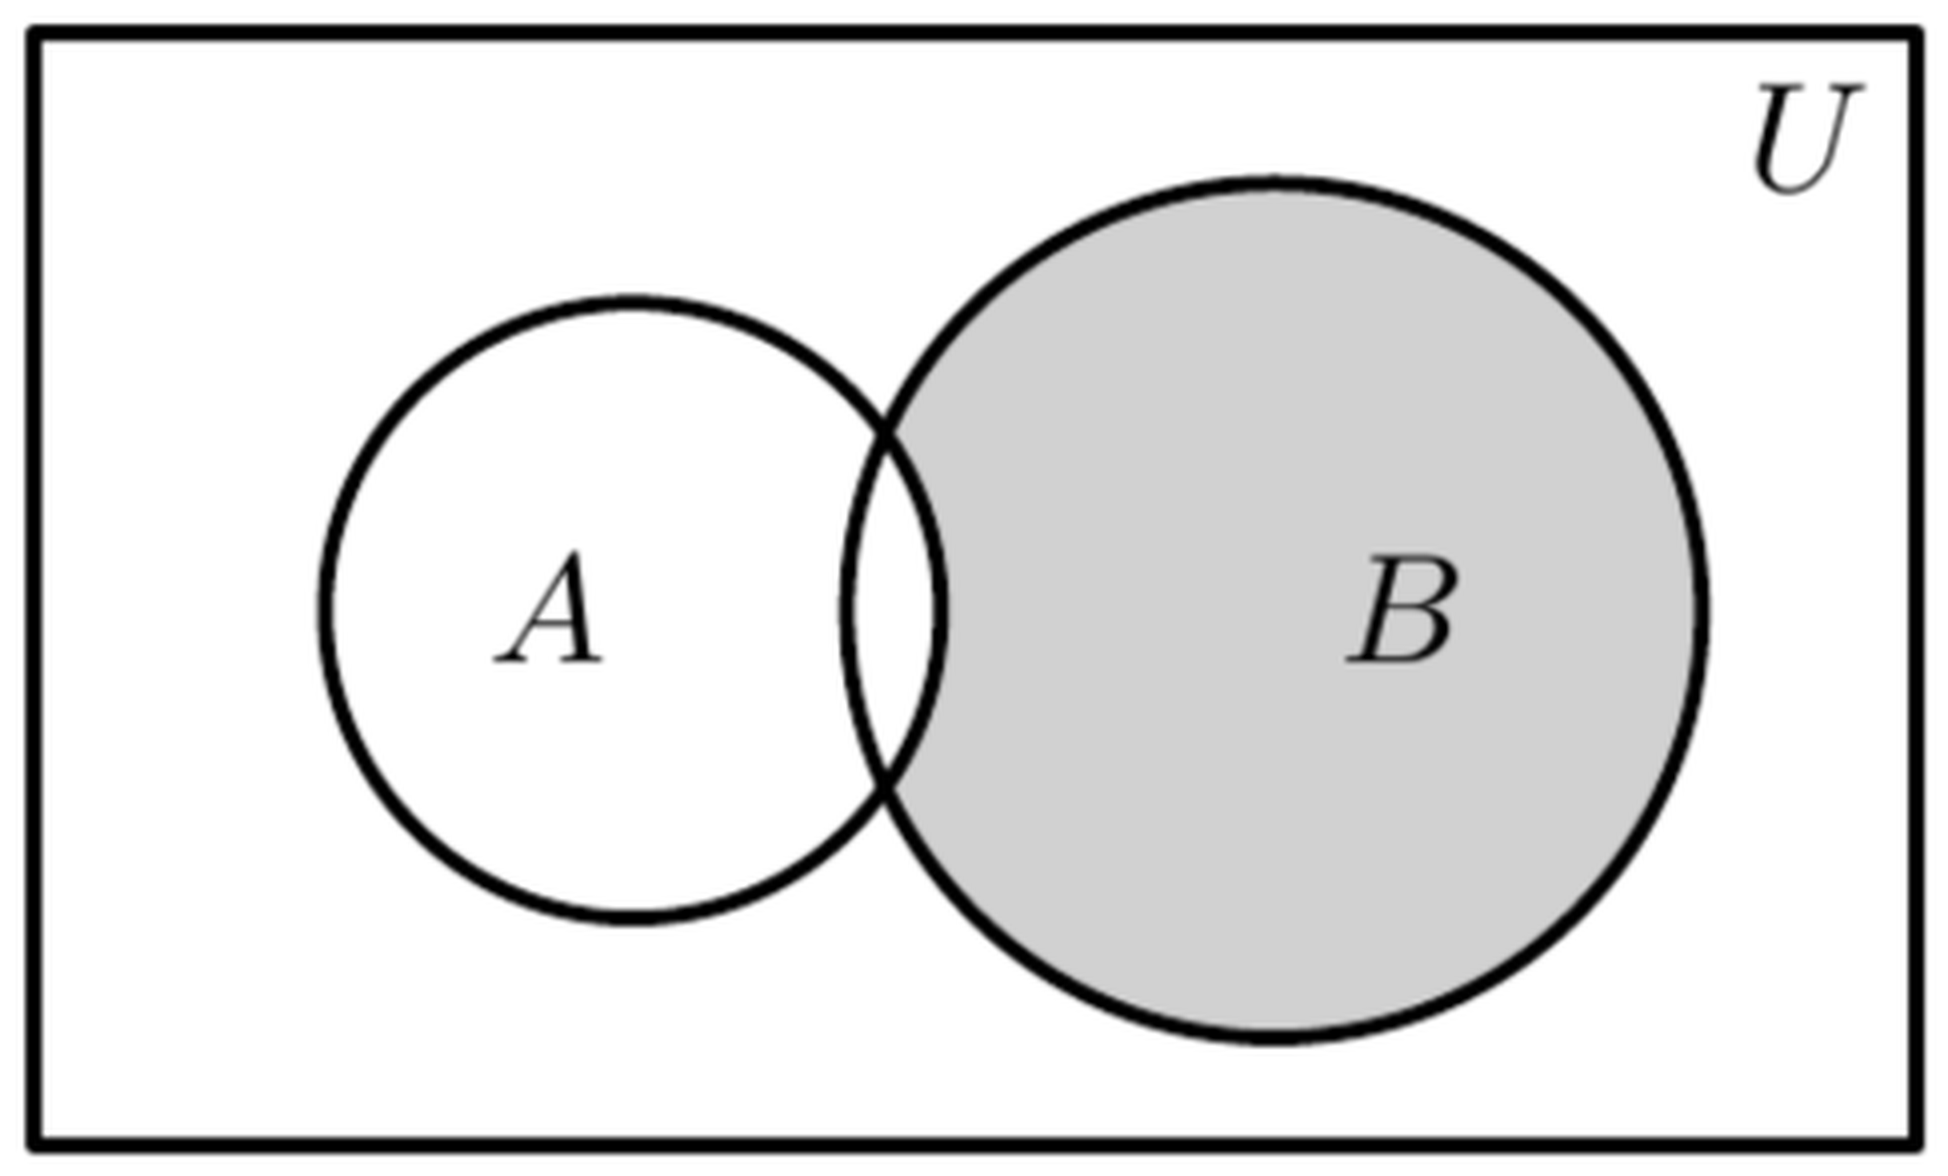
\includegraphics[width=0.38\textwidth]{figures/gao160_q4.png}
\end{center}

\ifanswer
\solbegin
\step{阴影部分表示 $B\cap\overline{A}=\{1,2\}$.}
\solend
\fi

% === Q5 === "图像"（有亻）照录；解析 1 行
\item 已知常数 $a>0$ 且 $a\ne1$，假设无论 $a$ 取何值，函数 $y=\log_a(5x-9)-4$ 的图像恒过一个定点，则这个定点的坐标为\blankline[4.4em].

\ifanswer
\solbegin
\step{$5x-9=1\Rightarrow x=2$，此时 $y=\log_a 1-4=-4$，定点为 $(2,-4)$.}
\solend
\fi

% === Q6 === 解析 2 行
\item 不等式 $(1-2x)^{\frac{3}{4}}>x^{\frac{3}{4}}$ 的解集为\blankline[4.4em].

\ifanswer
\solbegin
\step{定义域为 $\left[0,\dfrac{1}{2}\right]$，由幂函数的单调性，原不等式等价于 $1-2x>x$，}
\step{得 $0\leqslant x<\dfrac{1}{3}$，故解集为 $\left[0,\dfrac{1}{3}\right)$.}
\solend
\fi

% === Q7 === 绝对值 \lvert…\rvert；解析 2 行（跨 01—02 页）
\item 已知不等式 $\lvert x+3\rvert+\lvert x-2\rvert\geqslant 5$，当其等号成立时，$x$ 的取值范围是\blankline[4.4em].

\ifanswer
\solbegin
\step{$\lvert x+3\rvert+\lvert x-2\rvert=\lvert x+3\rvert+\lvert 2-x\rvert\geqslant\lvert(x+3)+(2-x)\rvert=5$，}
\step{等号成立当且仅当 $(x+3)(2-x)\geqslant0$，即 $x\in[-3,2]$.}
\solend
\fi

% === Q8 === 解析 4 行
\item 已知函数 $f(x)=\lvert\log_2 x\rvert$，若方程 $f(x)-t=0$ 有两个不同的实数根 $x_1,x_2$，则 $x_1+x_2$ 的取值范围是\blankline[4.4em].

\ifanswer
\solbegin
\step{方程有两个不同实根，必有 $t>0$，两根为 $2^t,2^{-t}$，}
\step{所以 $x_1+x_2=2^t+2^{-t}>2$（等号仅在 $t=0$ 时成立）.}
\step{任取 $s>2$，令 $a=\dfrac{s+\sqrt{s^2-4}}{2}>1$，取 $t=\log_2 a>0$，则 $x_1+x_2=a+\dfrac{1}{a}=s$，}
\step{所以取值范围为 $(2,+\infty)$.}
\solend
\fi

% === Q9 === 中文弯引号、\R、绝对值 \lvert…\rvert；解析 4 行
\item 已知 $a\in\R$，$b\in\R$，$p:\dfrac{1}{\lvert a\rvert}>\dfrac{1}{\lvert b\rvert}$，$q:\dfrac{1}{a}>\dfrac{1}{b}$，则 $p$ 是 $q$\blankline[4.4em]条件（用“充分非必要”、“必要非充分”、“充要”或“既非充分又非必要”填空）.

\ifanswer
\solbegin
\step{由 $p$、$q$ 中的分式有意义，$a\ne0$ 且 $b\ne0$.}
\step{当 $a=-1,b=-2$ 时，$p$ 成立而 $q$ 不成立，故 $p$ 不是 $q$ 的充分条件.}
\step{当 $a=1,b=-1$ 时，$q$ 成立而 $p$ 不成立，故 $p$ 不是 $q$ 的必要条件.}
\step{故 $p$ 是 $q$ 的充分非必要条件.}
\solend
\fi

% === Q10 === 解析 3 行；其后独立【注】按语 5 行（见头注 ② ⑯、⑤ 1）
\item 已知常数 $a>0$，函数 $y=\dfrac{2^x}{2^x+ax}$ 的图像经过点 $P\left(p,\dfrac{5}{6}\right)$、$Q\left(q,\dfrac{1}{6}\right)$，若 $2^{p+q}=3pq$，则 $a=$\blankline[4.4em].

\ifanswer
\solbegin
\step{由 $\dfrac{2^p}{2^p+ap}=\dfrac{5}{6}$ 得 $2^p=5ap$；由 $\dfrac{2^q}{2^q+aq}=\dfrac{1}{6}$ 得 $2^q=\dfrac{aq}{5}$.}
\step{$2^p>0$，$2^q>0$，$a>0$，得 $p>0$，$q>0$.}
\step{两式相乘得 $2^{p+q}=a^2pq$，又 $2^{p+q}=3pq$ 且 $pq\ne0$，故 $a^2=3$，$a=\sqrt{3}$.}
\solend
% 【注】按语（讲评版编者按，5 个印刷行，仅答案版出，不属于任何题的【解析】）
\stepm{【注】}{按原卷数据严格推敲，点 $Q$ 其实不存在：$a=\sqrt{3}$ 时 $2^q=\dfrac{\sqrt{3}}{5}q<q$；而当 $q>0$}
\step{时，取非负整数 $n$ 使 $n\leqslant q<n+1$，由 $2^{k+1}=2^k+2^k\geqslant2^k+1$ 逐次推得 $2^n\geqslant n+1$，于是}
\step{$2^q\geqslant2^n\geqslant n+1>q$，矛盾. 所以题设条件互相矛盾，严格说本题无解；$\sqrt{3}$ 是由题给关}
\step{系直接推出的值，按命题意图作为答案. 原卷数据疑似有误（同型常见题为 $P\left(p,\dfrac{6}{5}\right)$、}
\step{$Q\left(q,-\dfrac{1}{5}\right)$、$2^{p+q}=36pq$，得 $a=6$）.}% 见头注 ⑤ 1，照录未改
\fi

% === Q11 === 纳皮尔对数材料题；\Z、大数；解析 6 行
\item 17 世纪初，约翰·纳皮尔为了简化计算而发明了对数. 对数的发明是数学史上的重大事件，恩格斯曾经把笛卡尔的坐标系、纳皮尔的对数、牛顿和莱布尼兹的微积分共同称为 17 世纪的三大数学发明. 我们知道，任何一个正实数 $N$ 可以表示成 $N=a\times10^n$ ($1\leqslant a<10,n\in\Z$) 的形式，这便是科学记数法，若两边取常用对数，有 $\lg N=n+\lg a$，则可以估计 $3^{2026}$ 的最高位上的数值为\blankline[4.4em].

\ifanswer
\solbegin
\step{设 $3^{2026}=a\times10^n$ ($1\leqslant a<10,n\in\Z$)，则 $2026\lg 3=n+\lg a$.}
\step{用 $\lg 3\approx 0.4771$ 粗估，得 $2026\lg 3\approx 966.60$.}
\step{为核验误差，用 $0.47712<\lg 3<0.47713$，}
\step{得 $966.64512<2026\lg 3<966.66538$，因此 $n=966$.}
\step{于是 $\lg 4\approx 0.60206<0.64512<\lg a<0.66538<\lg 5\approx 0.69897$，}
\step{所以 $4<a<5$，最高位为 4，估算误差不影响结论.}
\solend
\fi

% === Q12 === 自定义"性质 P"；文本圈数字①②③；解析 19 行（跨 03—05 页）
\item 对于数集 $X=\{-1,x_1,x_2,x_3,\cdots,x_n\}$，其中 $0<x_1<x_2<x_3<\cdots<x_n$，$n\geqslant2$，定义点集 $Y=\{(s,t)\mid s\in X,t\in X\}$，若对于任意 $(s_1,t_1)\in Y$，存在 $(s_2,t_2)\in Y$，使得 $s_1s_2+t_1t_2=0$，则称集合 $X$ 具有性质 $P$. 则下列命题中为真命题的是\blankline[4.4em].

① $X=\{-1,1,2\}$ 具有性质 $P$；②若集合 $X$ 具有性质 $P$，则 $1\in X$；

③集合 $X$ 具有性质 $P$，若 $x_1=\dfrac{1}{2}$，则 $x_n=2$.

\ifanswer
\solbegin
\step{因为 $X=\{-1,1,2\}$，}
\step{所以 $Y=\{(-1,-1),(1,1),(2,2),(-1,1),(-1,2),(1,-1),(1,2),(2,-1),(2,1)\}$，}
\step{由集合 $X$ 具有性质 $P$ 的定义，对于任意 $(s,t)\in Y$，}
\step{若 $s>0$，$t>0$，则 $s=t$ 或 $(s,t)=(1,2)$ 或 $(s,t)=(2,1)$，}
\step{若 $s=t$，取 $s_2=-1$，$t_2=-1$，则 $ss_2+tt_2=0$；}
\step{若 $(s,t)=(1,2)$，取 $s_2=2$，$t_2=-1$，则 $ss_2+tt_2=0$；}
\step{若 $(s,t)=(2,1)$，取 $s_2=-1$，$t_2=2$，则 $ss_2+tt_2=0$；}
\step{若 $s$、$t$ 有一个为负数，则 $s=-1$ 或 $t=-1$，}
\step{若 $s=-1$，则取 $s_2=t$，$t_2=1$，则 $ss_2+tt_2=0$；}
\step{若 $t=-1$，则取 $s_2=1$，$t_2=s$，则 $ss_2+tt_2=0$；故①正确；}
\step{对于任意 $(s_1,t_1)\in Y$，存在 $(s_2,t_2)\in Y$，使得 $s_1s_2+t_1t_2=0$，}
\step{取 $(x_1,x_1)\in Y$，存在 $(x_p,x_q)$ 使得 $x_1x_p+x_1x_q=0$，所以 $x_p+x_q=0$，}
\step{不妨设 $x_p=1$，$x_q=-1$，所以若集合 $X$ 具有性质 $P$，则 $1\in X$，故②正确；}
\step{③假设 $x_n>1$，令 $s_1=\dfrac{1}{2},t_1=x_n$，则存在 $s$、$t\in X$ 使得 $\dfrac{1}{2}s+tx_n=0$，}
\step{同②得 $s$、$t$ 中必有一个数为 $-1$，}
\step{若 $s=-1$，则 $tx_n=\dfrac{1}{2}$，于是 $t=\dfrac{1}{2x_n}<\dfrac{1}{2}=x_1$，矛盾，}
\step{若 $t=-1$，则 $\dfrac{1}{2}s=x_n\cdot(-1)$，于是 $s=2x_n>x_n$，也矛盾，}% 原卷如此（与结论符号不自洽），照录未改，见头注 ⑤ 2
\step{所以 $x_n\leqslant1$，又由②得 $1\in X$，所以 $x_n\geqslant1$，所以 $x_n=1$，故③错误，}
\step{故真命题是①②.}
\solend
\fi

\end{enumerate}

% 答案版里填空解析把页排满，节标题会落到页末、与第 13 题分家（切页审计 B 类）；
% 守卫放 \bigsec 之前，连节标题一起量页高（高一157 成例）
\needvspace{7cm}
\bigsec{二、选择题}

\begin{enumerate}
\setcounter{enumi}{12}

% === Q13 === "图像"照录；解析 1 行，故选 $B$
\item 下列函数中，图像与函数 $y=3^x$ 图像关于 $y$ 轴对称的是\mbox{（\quad）}

\keepwithprev
A. $y=x^3$\qquad B. $y=\left(\dfrac{1}{3}\right)^x$\qquad C. $y=-3^x$\qquad D. $y=\log_3 x$

\ifanswer
\solbegin
\step{将 $x$ 换为 $-x$，得对称图像对应的函数为 $y=3^{-x}=\left(\dfrac{1}{3}\right)^x$，故选 $B$.}
\solend
\fi

% === Q14 === 中文弯引号；解析 2 行（跨 05 页上下），故选 $B$
\item 命题“存在 $x\in(1,+\infty)$，使得 $f(x)>0$”的否定形式为\mbox{（\quad）}

\keepwithprev
A. 不存在 $x\in(-\infty,1]$，使得 $f(x)>0$\qquad B. 对任意 $x\in(1,+\infty)$，有 $f(x)\leqslant0$

C. 对任意 $x\in(-\infty,1]$，有 $f(x)\leqslant0$\qquad D. 存在 $x\in(1,+\infty)$，使得 $f(x)\leqslant0$

\ifanswer
\solbegin
\step{将“存在”改为“对任意”，$x$ 的范围不变，并将 $f(x)>0$ 否定为 $f(x)\leqslant0$，}
\step{故选 $B$.}
\solend
\fi

% === Q15 === \R；四选项两行；解析 3 行，故选 $D$
\item 设 $a>0$，$s\in\R$. 下列各项中，能推出 $a^s>a$ 的一项是\mbox{（\quad）}

\keepwithprev
A. $a>1$，且 $s>0$\qquad B. $a>1$，且 $s<0$

C. $0<a<1$，且 $s>0$\qquad D. $0<a<1$，且 $s<0$

\ifanswer
\solbegin
\step{当 $a>1$ 时，$a^s>a\Leftrightarrow s>1$，A、B 均不能保证.}
\step{当 $0<a<1$ 时，$a^s>a\Leftrightarrow s<1$，C 不能保证，D 中 $s<0<1$，满足要求；}
\step{故选 $D$.}
\solend
\fi

% === Q16 === 题目配图（三版都出）；几何符号 \triangle ABC；解析 3 行，故选 $C$
\needvspace{8cm}
\item 数学说明的方法多种多样，其中利用图形说明就是一种重要方法. 如图所示，在等腰直角三角形 $\triangle ABC$ 中，点 $O$ 为斜边 $AB$ 的中点，点 $D$ 为斜边 $AB$ 上异于顶点的一个动点，设 $AD=a$，$BD=b$，则可用该图形能说明的不等式为\mbox{（\quad）}

\begin{center}
% Q16 等腰直角三角形 ABC 图（C/A/O/D/B 标注）取 05 页右下，去粉色水印、去色、3× LANCZOS 放大；三版都出
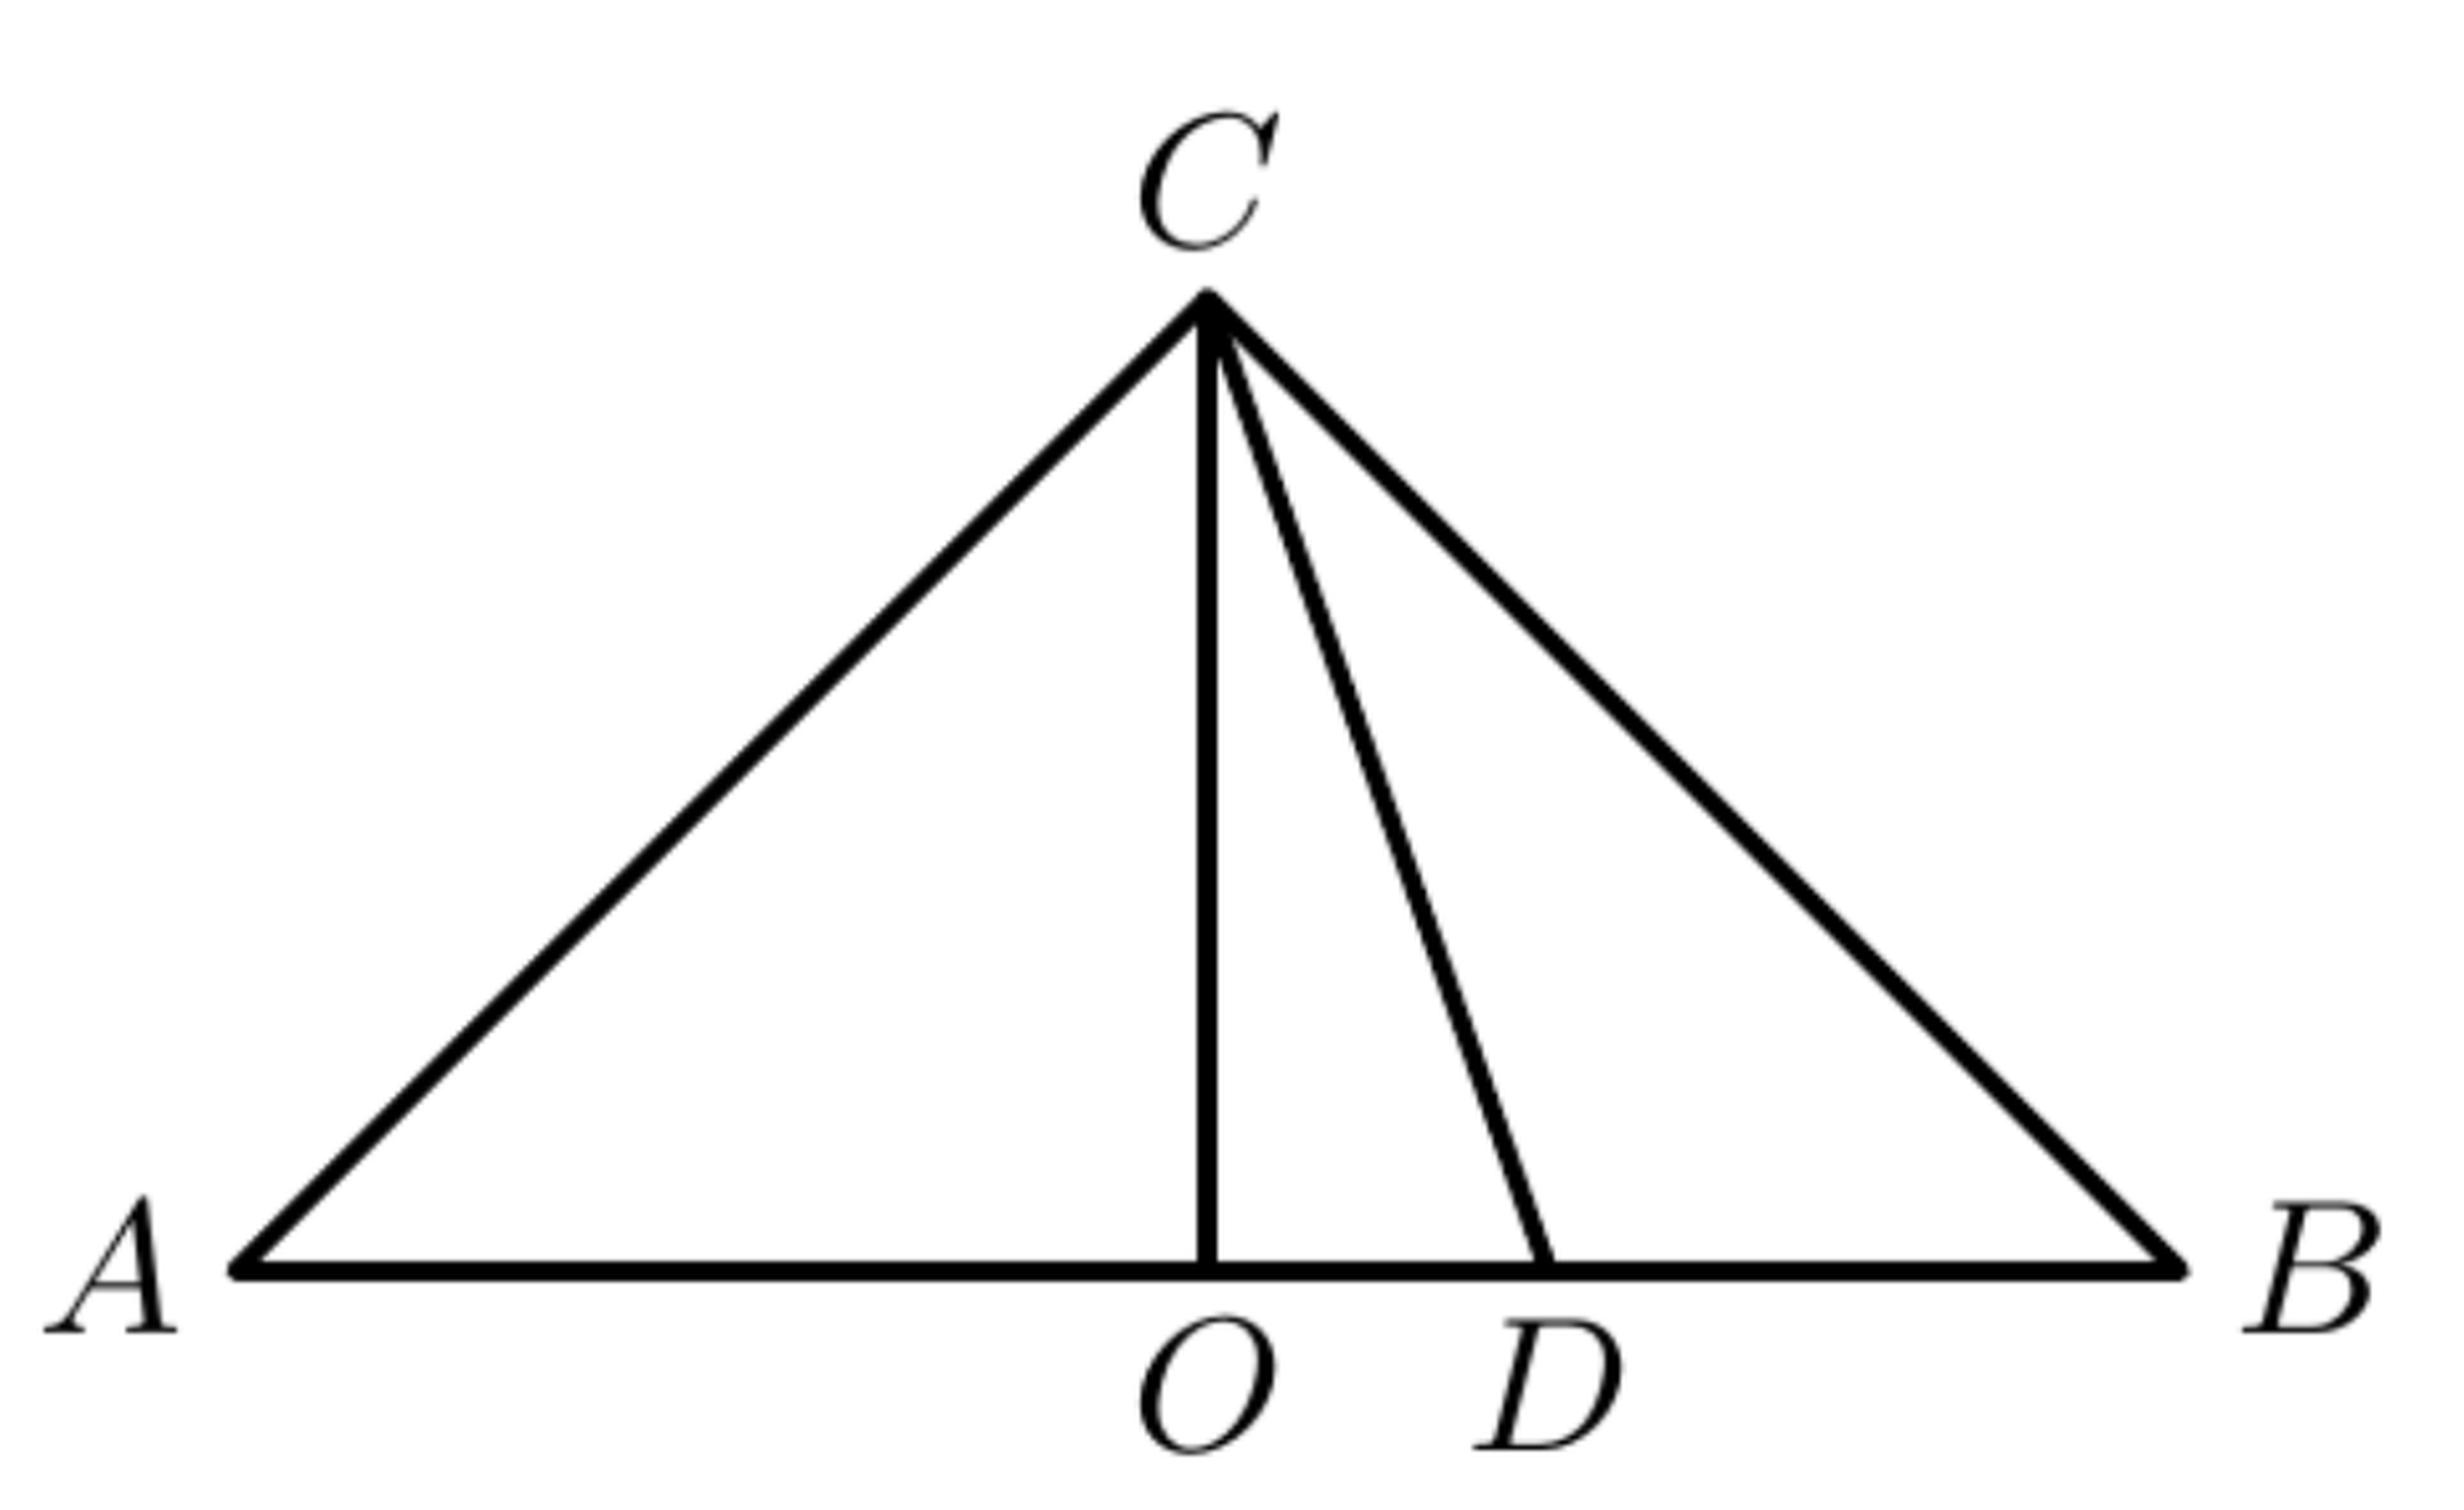
\includegraphics[width=0.34\textwidth]{figures/gao160_q16.png}
\end{center}

\keepwithprev
A. $\dfrac{a+b}{2}\geqslant\sqrt{ab}$ ($a>0,b>0$)\qquad B. $a^2+b^2\geqslant2\sqrt{ab}$ ($a>0,b>0$)

C. $\dfrac{a+b}{2}\leqslant\sqrt{\dfrac{a^2+b^2}{2}}$ ($a>0,b>0$)\qquad D. $\dfrac{2ab}{a+b}\leqslant\sqrt{ab}$ ($a>0,b>0$)

\ifanswer
\solbegin
\step{$CO=AO=\dfrac{a+b}{2},OD=\left\lvert a-\dfrac{a+b}{2}\right\rvert=\dfrac{\lvert a-b\rvert}{2}$，}
\step{$CD=\sqrt{CO^2+OD^2}=\sqrt{\dfrac{a^2+b^2}{2}}\geqslant CO=\dfrac{a+b}{2}$，}
\step{等号当且仅当 $a=b$ 时成立，故选 $C$.}
\solend
\fi

\end{enumerate}

\bigsec{三、解答题}

\begin{enumerate}
\setcounter{enumi}{16}

% === Q17 === cases 块算一行；判别式印等腰偏高三角 \Delta；解析 7 行
\item 已知幂函数 $f(x)=(m^2-2m-2)x^{m-1}$ 在 $(0,+\infty)$ 上是严格增函数.

(1) 求 $m$ 的值；

(2) 若关于 $x$ 的方程 $f(x)=(t+1)x-t^2$ 有两个不相等的正实根，求实数 $t$ 的取值范围.

\ifanswer
\solbegin
\step{(1) 幂函数的系数为 1，因此 $m^2-2m-2=1\Leftrightarrow(m-3)(m+1)=0$，}
\step{解得 $m=3$ 或 $m=-1$.}
\step{由 $f(x)$ 在 $(0,+\infty)$ 上严格递增，得 $m-1>0$，所以 $m=3$，}
\step{此时 $f(x)=x^2$.}
\step{(2) 原方程化为 $x^2-(t+1)x+t^2=0$，}
\step{方程有两个不相等的正实根，则 $\begin{cases}\Delta=(t+1)^2-4t^2=(1-t)(3t+1)>0\\t+1>0\\t^2>0\end{cases}$，}% 判别式原卷印等腰偏高三角 \Delta，照录
\step{得 $t\in\left(-\dfrac{1}{3},0\right)\cup(0,1)$.}
\solend
\fi

% === Q18 === 补集上划线 \overline{A}、\subseteq 带下划线、\varnothing；解析 8 行
\item 已知集合 $A=\{x\mid\lvert x-a\rvert<a-3\}$，$B=\left\{x\mid\dfrac{x+1}{x-2}\geqslant2\right\}$.

(1) 若 $a=5$，求 $\overline{A}\cap B$；

(2) 若 $A\cap B=A$，求实数 $a$ 的取值范围.

\ifanswer
\solbegin
\step{(1) $\dfrac{x+1}{x-2}\geqslant2\Leftrightarrow\dfrac{5-x}{x-2}\geqslant0\Leftrightarrow2<x\leqslant5,B=(2,5]$，}
\step{当 $a=5$ 时，$A=\{x\mid\lvert x-5\rvert<2\}=(3,7)$，于是 $\overline{A}=(-\infty,3]\cup[7,+\infty)$，}
\step{因此 $\overline{A}\cap B=(2,3]$.}
\step{(2) $A\cap B=A$ 等价于 $A\subseteq B$.}
\step{当 $a\leqslant3$ 时，$a-3\leqslant0$，$A=\varnothing$，满足条件.}
\step{当 $a>3$ 时，$\lvert x-a\rvert<a-3\Leftrightarrow3<x<2a-3,A=(3,2a-3)$，}
\step{此时 $A\subseteq B=(2,5]$ 等价于 $2a-3\leqslant5$，即 $a\leqslant4$，结合 $a>3$ 得 $3<a\leqslant4$.}
\step{合并两种情形，实数 $a$ 的取值范围为 $(-\infty,4]$.}
\solend
\fi

% === Q19 === 数据表 tabular 重排（高一130 成例）；cases 块算一行；解析 6 行
\item 作为我国最高水平的综合性运动会，全运会汇聚了国内顶尖体育健儿，某代表队从第 8 届全运会开始登上赛场，且参赛运动员人数逐年递增. 设 $t$ 为该代表队参赛后经过的届数，即第 8 届为 $t=0$，第 9 届为 $t=1$，以此类推. 经过 $t$ 届，运动员人数为 $y$ 人，具体数据如下：

\begin{center}
\begin{tabular}{cccccc}
$t$ & 0 & 1 & 2 & 3 & 4 \\
\hline
届数 & 8 & 9 & 10 & 11 & 12 \\
运动员人数（$y$ 人） & 4 & 11 & 25 & 53 & 109
\end{tabular}
\end{center}

(1) 现有以下两种函数模型：① $y=a\cdot b^t+c$ ($a>0,b>1$)；② $y=\log_a(t+b)+c$ ($b>0,a>1$). 请根据上表中运动员人数的增长规律，选出你认为符合的函数模型（不用说明理由），并利用表中前 3 组数据求出相应的函数解析式；

(2) 若参赛运动员人数按照 (1) 中求得的模型继续增长，在第几届全运会时，该代表队运动员人数将会首次超过 1000 人？

\ifanswer
\solbegin
\step{(1) 选模型①，将前 3 组数据代入，得 $\begin{cases}a+c=4\\ab+c=11\\ab^2+c=25\end{cases}$，}% 原卷印"选模型①"（圈数字①），OCR 误作"四"，照录①，见头注 ⑤ 3
\step{相邻两式相减，得 $a(b-1)=7$，$ab(b-1)=14$，}
\step{两式相除得 $b=2$，进而 $a=7$，$c=-3$，所求函数解析式为 $y=7\cdot2^t-3$.}
\step{(2) $y=7\cdot2^t-3$ 随 $t$ 的增大而增大，且 $t=7$ 时，$y=893<1000$；}
\step{$t=8$ 时，$y=1789>1000$，}
\step{$t$ 为非负整数，首次超过 1000 人时 $t=8$，对应第 $8+8=16$ 届全运会.}
\solend
\fi

% === Q20 === 解析 12 行（跨 08—09 页）
\item 已知函数 $f(x)=\log_a(a-a^x)$.

(1) 求该函数的定义域；

(2) 若 $a>1$，试判断关于 $x$ 的方程 $f(x)=2$ 是否有实数解，并说明理由；

(3) 若当 $x\in(-\infty,0]$ 时，关于 $x$ 的不等式 $f(x)\geqslant-1$ 恒成立，求实数 $a$ 的取值范围.

\ifanswer
\solbegin
\step{(1) 对数的底数须满足 $a>0$ 且 $a\ne1$，真数须满足 $a-a^x>0$，即 $a^x<a^1$.}% 原卷印 $a^1$，照录未化简，见头注 ⑤ 4
\step{当 $a>1$ 时，$x<1$，定义域为 $(-\infty,1)$.}
\step{当 $0<a<1$ 时，$x>1$，定义域为 $(1,+\infty)$.}
\step{(2) 当 $a>1$ 时，若 $f(x)=2$，则 $a-a^x=a^2\Rightarrow a^x=a(1-a)<0$，}
\step{这与 $a^x>0$ 矛盾，因此方程无实数解.}
\step{(3) 不等式在 $(-\infty,0]$ 上恒成立，须先保证该区间包含于函数的定义域，}
\step{由 (1) 得 $a>1$.}
\step{当 $x\leqslant0$ 时，$0<a^x\leqslant1$，所以 $a-a^x\geqslant a-1>0$.}
\step{由对数函数的单调性，$f(x)=\log_a(a-a^x)\geqslant\log_a(a-1)=f(0)$，}
\step{等号当且仅当 $x=0$ 时成立，}
\step{因此所求条件等价于 $\log_a(a-1)\geqslant-1\Leftrightarrow a-1\geqslant\dfrac{1}{a}\Leftrightarrow a^2-a-1\geqslant0$，}
\step{结合 $a>1$，得 $a\in\left[\dfrac{1+\sqrt{5}}{2},+\infty\right)$.}
\solend
\fi

% === Q21 === "和积平衡集"定义证明题；\N；解析 18 行（跨 09—10 页）
\item 已知有限集 $A=\{a_1,a_2,\cdots,a_n\}$ ($n\geqslant2,n\in\N$)，如果 $A$ 中元素 $a_i$ ($i=1,2,3,\cdots,n$) 满足 $a_1+a_2+a_3+\cdots+a_n=a_1\times a_2\times\cdots\times a_n$，就称 $A$ 为“和积平衡集”.

(1) 分别判断集合 $A=\{1,2,3,4\}$，$B=\{4+2\sqrt{2},4-2\sqrt{2}\}$ 是否为“和积平衡集”；

(2) 已知 $a_1$、$a_2$ 是两个不同的正数，且 $\{a_1,a_2\}$ 是“和积平衡集”，请用反证法证明：$a_1$、$a_2$ 至少有一个大于 2；

(3) 若 $a_i\geqslant1$，且 $a_i\in\N$，求所有符合条件的“和积平衡集”.

\ifanswer
\solbegin
\step{(1) 因为 $1+2+3+4=10\ne24=1\times2\times3\times4$，所以 $A$ 不是“和积平衡集”.}
\step{因为 $(4+2\sqrt{2})+(4-2\sqrt{2})=8=(4+2\sqrt{2})(4-2\sqrt{2})$，}
\step{所以 $B$ 是“和积平衡集”.}
\step{(2) 假设 $a_1$、$a_2$ 都不大于 2，则 $\dfrac{1}{a_1}\geqslant\dfrac{1}{2},\dfrac{1}{a_2}\geqslant\dfrac{1}{2}$，}
\step{由于 $a_1\ne a_2$，上述两个不等式至少有一个严格成立.}
\step{而 $a_1+a_2=a_1a_2$，两边除以 $a_1a_2>0$，得 $1=\dfrac{1}{a_1}+\dfrac{1}{a_2}>\dfrac{1}{2}+\dfrac{1}{2}=1$，矛盾，}
\step{所以 $a_1$、$a_2$ 至少有一个大于 2.}
\step{(3) 不妨设 $a_1<a_2<\cdots<a_n$，由各元素均为正整数，得 $a_i\geqslant i$.}
\step{若 $n\geqslant4$，因其余因子均不小于 1，}
\step{有 $a_1a_2\cdots a_n\geqslant a_2a_{n-1}a_n\geqslant2(n-1)a_n>na_n>a_1+a_2+\cdots+a_n$，}
\step{与和积平衡条件矛盾，因此只需讨论 $n=2,3$.}
\step{当 $n=2$ 时，$a_1+a_2=a_1a_2\Leftrightarrow(a_1-1)(a_2-1)=1$，}
\step{两个因子均为非负整数，只能有 $a_1=a_2=2$，与元素互不相同矛盾.}
\step{当 $n=3$ 时，若 $a_1\geqslant2$，则 $a_2\geqslant3$，从而 $a_1a_2a_3\geqslant6a_3>3a_3>a_1+a_2+a_3$，}
\step{矛盾，因此 $a_1=1$.}
\step{此时 $1+a_2+a_3=a_2a_3\Leftrightarrow(a_2-1)(a_3-1)=2$，}
\step{由 $1\leqslant a_2-1<a_3-1$，得 $a_2-1=1$、$a_3-1=2$，即 $a_2=2$、$a_3=3$.}
\step{检验 $1+2+3=1\times2\times3=6$，所求集合为 $\{1,2,3\}$.}
\solend
\fi

\end{enumerate}

\end{document}
"
% 紧凑版：xelatex "\def\iscompact{1}% 高一160_奉贤中学_期中.tex
%   —— 高一上数学"2026-2027 年奉贤中学高一上期中"（试卷版/答案版/紧凑版）
% 试卷版：xelatex 高一160_奉贤中学_期中.tex
% 答案版：xelatex "\def\isanswer{1}\input{高一160_奉贤中学_期中.tex}"
% 紧凑版：xelatex "\def\iscompact{1}\input{高一160_奉贤中学_期中.tex}"
%
% ① 原始材料：微信公众号"魔都数学加油站"文章，连载"27学年高一160"，原卷卷面标题
% "2026-2027 年奉贤中学高一上期中"（卷面未印副标题、未印连载号）。
% 正文为 10 张 PNG 页（01/04/10 为 2560×3620，02/03/05/06/07/08/09 为
% 4762×6735，同一篇各页分辨率混排，逐页按各自分辨率裁图核对）。
% 体例：讲评版——填空 3—12（10 题）、选择 13—16（4 题）、解答 17—21（5 题），
% 共 19 题，自第 3 题起编（1、2 未印在本篇）；19 题逐题印【解析】，无只印【答案】
% 的题；四道选择题答案在解析末句"故选 $B$/$B$/$D$/$C$"，题干括号
% \mbox{（\quad）} 留空、不另提 \ans{}。题目、答案、解析均据原图转录；卷面粉红色
% 水印"魔都数学加油站"及公众号页脚未录入。
% 全卷插图清单（逐页通读 10 页确认）：2 幅，均为题目配图、三版都出——
%   · Q4 韦恩图（01 页右侧：矩形全集 U、两圆 A/B、阴影部分 B∩上划线 A、
%     标注 U/A/B），裁 figures/gao160_q4.png；
%   · Q16 等腰直角三角形 ABC 图（05 页右下：C 顶点、A/O/D/B 共线底边、
%     CO 与 CD 两条线段），裁 figures/gao160_q16.png；
%   两图均取原卷截图 3—4× LANCZOS 放大、去粉色水印、转灰度、autocontrast；
%   Q4 图左侧题干残字"示"、Q16 图左侧题干残字均已裁白。
%   Q19 有一张 3 行数据表（t／届数／运动员人数（y 人），t=0..4），按全稿
%   成例（高一130）用 tabular 重排，不做成 png；其余各页无题目配图、
%   无解析内配图、无其它表格、无"如图"处。
%
% 卷首标题：原卷印作"2026-2027 年奉贤中学高一上期中"，年份区间按全稿惯例排 en dash；
% 原卷卷面未印副标题，本稿按同期中卷知识模块口径补出"集合与常用逻辑用语、不等式、函数"。
%
% ② 与原卷的排版差异／照录项清单：
%   ① 原文从第 3 题起，本稿保留原题号；共 19 题三节，解答题 5 题到 21；
%      三节各自一个 enumerate + \setcounter{enumi}{2}/{12}/{16}（不贯穿），
%      用 \examtitlest[3] 起手；
%   ② 混合体例说明：19 题全印【解析】、用 \solbegin…\solend，无只印【答案】
%      或答案印括号内的题；四道选择题答案在解析末句"故选 $B$/$B$/$D$/$C$"
%      （逐个放大复核）、括号 \mbox{（\quad）} 留空、不另提 \ans{}；答案版
%      【答案】/【解析】标记数 = 19 = 全卷题数（0 个 \ans ＋ 19 个 \solbegin）；
%   ③ 原卷卷面未印副标题，本稿按知识模块口径补出；
%   ④ 原卷填空横线按全稿惯例排 \blankline[4.4em]；选择题括号排 \mbox{（\quad）}、
%      四道选择题的选项段前按惯例各加 \keepwithprev；解答题不留作答区、不加
%      \anspace（原卷为讲评版，109—113 起全稿不用 \anspace）；
%   ⑤ 数集归一：Q4"$U=\Z$"、Q9"$a\in\R$，$b\in\R$"、Q11"$n\in\Z$"、
%      Q15"$s\in\R$"、Q21"$n\in\N$""$a_i\in\N$"原卷印正体粗体 Z/R/N，
%      按全稿惯例归一 \Z／\R／\N；集合描述竖线排 \mid（Q3、Q4、Q12、
%      Q18、Q21）；空集 \varnothing（Q18 解析 (2)）；补集照原卷上划线排
%      \overline{A}（Q4 解析、Q18 (1) 题干与解析）；子集符号 Q18 两处
%      "$A\subseteq B$"印带下划线 ⊆、照录 \subseteq；
%   ⑥ 绝对值排 \lvert…\rvert（Q7、Q8 题干与解析、Q9 题干、Q16 解析、
%      Q18 题干与解析），Q16 解析的 \left\lvert…\right\rvert 与 \lvert…\rvert
%      均在同一 $…$ 组内配对平衡；
%   ⑦ 判别式两形混用逐处照录不统一（放大逐处确认）：Q3 解析
%      "$\triangle=1^2-4a\times\frac{1}{4}=0$"原卷印扁等边三角、照录
%      \triangle；Q17 解析 cases 块"$\Delta=(t+1)^2-4t^2=(1-t)(3t+1)>0$"
%      原卷印等腰偏高三角、照录 \Delta；Q16 题干几何符号"$\triangle ABC$"
%      按全稿几何三角形记号惯例归一 \triangle（参照 高一150／132 成例）；
%   ⑧ 不等号按全稿惯例排 \leqslant／\geqslant；中文弯引号照录：Q9 题干
%      "充分非必要""必要非充分""充要""既非充分又非必要"、Q14 题干
%      "存在 $x\in(1,+\infty)$，使得 $f(x)>0$"与解析"存在""对任意"、
%      Q21 题干与解析多处"和积平衡集"；注释里一律 ASCII 引号；
%   ⑨ 文本圈数字逐处照录：Q12 题干①②③、Q12 解析"故①正确""同②得"
%      "故②正确""③假设""故③错误""故真命题是①②"、Q19 题干①②与解析
%      "选模型①"，均为印刷圈数字（非 \textcircled、非数学模式）；
%   ⑩ 半角逗号在数学组之间是全稿惯例、非笔误，逐处照录（Q8"$2^t,2^{-t}$"、
%      Q9"$a=-1,b=-2$""$a=1,b=-1$"、Q11"$1\leqslant a<10,n\in\Z$"、
%      Q12"$s_1=\frac{1}{2},t_1=x_n$"、Q16 选项"$a>0,b>0$"与解析
%      "$CO=AO=\frac{a+b}{2},OD=...$"、Q18"$2<x\leqslant5,B=(2,5]$"
%      "$3<x<2a-3,A=(3,2a-3)$"、Q21"$n=2,3$"等）；行中全角逗号／顿号
%      照录（Q15 选项"$a>1$，且 $s>0$"、Q12 解析"$s$、$t$"、Q21 解析
%      "$a_1$、$a_2$"），顿号一律移出数学模式；
%   ⑪ "图像／图象"逐处照录：本卷 Q5"的图像恒过一个定点"、Q10"的图像经过点"、
%      Q13 题干两处"图像"与解析"对称图像对应的函数"均印"图像"（有亻）；
%      Q16 印"图形"（利用图形说明、该图形能说明），无"图象"用例；
%   ⑫ 复杂式照录别简化：Q3 $ax^2+x+\frac14=0$、Q5 $y=\log_a(5x-9)-4$、
%      Q6 $(1-2x)^{\frac34}>x^{\frac34}$ 与 $\left[0,\frac12\right]$、
%      Q8 $\frac{s+\sqrt{s^2-4}}{2}$、Q10 $y=\frac{2^x}{2^x+ax}$ 与
%      $\frac{2^p}{2^p+ap}=\frac56$、$\frac{2^q}{2^q+aq}=\frac16$、
%      Q11 $N=a\times10^n$ 与 $3^{2026}$、$2026\lg3\approx966.60$、
%      $966.64512<2026\lg3<966.66538$、Q12 $Y=\{(s,t)\mid s\in X,t\in X\}$
%      与 $\frac12 s+tx_n=0$、Q16 $\sqrt{\frac{a^2+b^2}{2}}$、
%      Q17 $x^2-(t+1)x+t^2=0$ 与 $\left(-\frac13,0\right)\cup(0,1)$、
%      Q18 $\frac{5-x}{x-2}\geqslant0$、Q19 $y=a\cdot b^t+c$ 与
%      $y=\log_a(t+b)+c$、$y=7\cdot2^t-3$、Q20 $f(x)=\log_a(a-a^x)$
%      与 $a^2-a-1\geqslant0$、$\left[\frac{1+\sqrt5}{2},+\infty\right)$、
%      Q21 $4+2\sqrt2$ 与 $(a_2-1)(a_3-1)=2$ 等；
%   ⑬ 子题标号 (1)(2)(3) 按全稿惯例排半角括号；行末／行中句点按全稿惯例
%      排 ASCII `.`（不是全角「．」）；cases 块整体算一个印刷行
%      （Q17 解析、Q19 解析 (1)）；
%   ⑭ 配图：Q4／Q16 题目配图（三版都出）放 \item 内题干之后 \begin{center}，
%      各用 \needvspace{8cm} 守卫把整块推走，**守卫放在 \item 之前**
%      （见 高一153 Q11/Q19 成例与切页审计 B 类坑）；
%   ⑮ 一条 \step = 原卷解析的一个印刷行；跨上下半页的重叠行只算一次
%      （Q4 解析、Q9 解析首行、Q11 解析首行、Q12 解析"若 $s=-1$…"一行、
%      Q18 解析"此时 $A\subseteq B=(2,5]$…"一行、Q20 (2) 题干、
%      Q21 解析"由 $1\leqslant a_2-1<a_3-1$…"一行）；原卷折行别合并；
%   ⑯ Q10 之后另有一整块【注】按语（03 页上半，5 个印刷行），是讲评版作者对
%      原卷数据自相矛盾的加注、不属于任何题的【解析】。本稿按 高一53
%      "注：…"成例放 Q10 的 \solend 之后、Q10 的 \fi 收尾之前：
%      **整块只保留 Q10 那一层外层 \ifanswer**（那个 \fi 就是 Q10 的收尾），
%      块内 \stepm{【注】}{首行} ＋ 4 条 \step 各自自带内层 \ifanswer…\fi
%      （\step／\stepm 宏内自带，源码里不手动再包一层 \ifanswer，
%      否则 题目溯源.py 的 strip_answers 非贪婪正则会错切）；
%      \stepm 第一参数直接用「【注】」作标签，与全稿 \ans 的【答案】、
%      \solbegin 的【解析】同性质，未加粗以外不另加任何样式；
%      5 行仅答案版出、不新增 \item、不影响溯源，头注 ③ 单列登记、
%      不计入 19 题逐题 \step 账；\stepm 把【注】排成加粗着色标签
%      （原卷为黑色加粗），此一处着色差异在此登记；
%   ⑰ 原卷用字照录：Q11"约翰·纳皮尔""莱布尼兹"（原卷作"兹"，非通行"茨"）、
%      "17 世纪的三大数学发明"；Q16"数学说明的方法""点 $D$ 为斜边 $AB$ 上
%      异于顶点的一个动点"；Q19"登上赛场""以此类推"；
%
% ③ 行数复核：一条 \step = 原卷解析的一个印刷行，cases 块作一个印刷行计。
%   逐题数（逐页核对定稿）：Q3：5；Q4：1；Q5：1；Q6：2；Q7：2；Q8：4；
%   Q9：4；Q10：3；Q11：6；Q12：19；Q13：1；Q14：2；Q15：3；Q16：3；
%   Q17：7；Q18：8；Q19：6；Q20：12；Q21：18。
%   合计 107 条 \step（19 题逐题印刷行账），与原卷逐题印刷行相等。
%   **本卷源码 \step 总数 = 19 题逐题合计 107 ＋ Q10 后独立【注】块 5 行
%   = 112 行**（其中 \step 111 条、\stepm 1 条；\stepm 与 4 条 \step 合为
%   【注】块 5 印刷行）。该 5 行不计入「逐题印刷行」账，也不是任何题的
%   【解析】，而是讲评版编者按语；主会话核验脚本按全文统计 \step 时总数会
%   较逐题账多 5，已与主会话对齐、属已知预期而非错误。
%   全卷 19 题均设 \solbegin…\solend，答案版【答案】/【解析】标记数
%   = 19 = 全卷题数。
%
% ④ 页码分布（供回原图复核）：
%   卷首标题＋"一、填空题"＋Q3 题干＋解析 5 行＋Q4 题干＋韦恩图＋解析
%   1 行＋Q5 题干首行在 01 页上半；Q4 解析（重叠）＋Q5 题干续＋解析 1 行＋
%   Q6 题干＋解析 2 行＋Q7 题干＋解析首行在 01 页下半；Q7 解析末行＋
%   Q8 题干＋解析 4 行＋Q9 题干＋解析首行在 02 页上半；Q9 解析（重叠首行）
%   ＋余 3 行＋Q10 题干＋解析 3 行在 02 页下半；【注】按语 5 行＋Q11 题干＋
%   解析首行在 03 页上半；Q11 解析（重叠首行）＋余 5 行＋Q12 题干＋①②
%   在 03 页下半；Q12 ③＋解析前 9 行在 04 页上半；Q12 解析（重叠 2 行）
%   ＋余 8 行在 04 页下半；Q12 解析末 2 行＋"二、选择题"＋Q13 题干＋选项＋
%   解析 1 行＋Q14 题干＋选项＋解析首行在 05 页上半；Q14 解析末行＋
%   Q15 题干＋选项＋解析 3 行＋Q16 题干＋三角形图在 05 页下半；
%   Q16 选项＋解析 3 行＋"三、解答题"＋Q17 题干＋两问在 06 页上半；
%   Q17 解析 7 行在 06 页下半；Q18 题干＋两问＋解析前 7 行＋Q19 题干首行
%   在 07 页上半；Q18 解析末行（重叠）＋Q19 题干＋表格＋两问在 07 页下半；
%   Q19 解析 6 行＋Q20 题干＋(1)(2) 在 08 页上半；Q20 (2)(3) 题干（重叠）
%   ＋解析 8 行在 08 页下半；Q20 解析末 4 行＋Q21 题干＋(1)(2) 在 09 页
%   上半；Q21 (3)＋解析前 7 行在 09 页下半；Q21 解析 (3) 余 10 行在 10 页
%   上半；Q21 末行（重叠）＋"检验 $1+2+3=1\times2\times3=6$，所求集合为
%   $\{1,2,3\}$."在 10 页下半（此后仅水印、无正文）。本稿按题连排，
%   不丢行、不并折行；全卷末题为第 21 题，无附加题节。
%
% ⑤ 存疑照录（放大原图确认，照录未改、正文对应处另有 % 注）：
%   1. Q10【注】按语：讲评版作者据 $a=\sqrt3$ 时 $2^q=\frac{\sqrt3}{5}q<q$
%      与 $2^n\geqslant n+1$ 推出点 $Q$ 不存在、"严格说本题无解"，并注明
%      "原卷数据疑似有误（同型常见题为 $P(p,\frac65)$、$Q(q,-\frac15)$、
%      $2^{p+q}=36pq$，得 $a=6$）"；本稿照录全块、未删未改（见 ② ⑯）。
%   2. Q12 解析 (3) 末段"若 $t=-1$，则 $\frac{1}{2}s=x_n\cdot(-1)$，
%      于是 $s=2x_n>x_n$，也矛盾，"中，等式右端与紧随的结论符号不自洽
%      （按题意应为 $\frac12 s=x_n$ 或 $-\frac12 s=x_n\cdot(-1)$），逐页
%      放大 04 页确认原卷即如此印、无漏看的负号，照录未改，建议主会话
%      回 04 页再放大复核一次；
%   3. Q19 解析 (1) 印"选模型①"（圈数字①，题干只有①②两种模型）；
%      OCR 误作"选模型四"，放大 08 页确认是①、照录①；
%   4. Q20 解析 (1)"即 $a^x<a^1$"末项原卷印 $a^1$（非 $a$），照录未化简；
%   5. Q11 题干"莱布尼兹"原卷作"兹"（非通行"茨"）、"约翰·纳皮尔"用
%      间隔号·，均照录未改；
%   6. Q9 题干"则 $p$ 是 $q$___条件"与解析"故 $p$ 是 $q$ 的充分非必要条件"
%      句式略异，均照录；
%   7. Q19 解析 (1) 用"前 3 组数据"、题干表格列到 $t=4$，照录未补。
%
\documentclass[a4paper,11pt]{article}
\usepackage{common}

\begin{document}

\examtitlest[3]{2026--2027 年奉贤中学高一上期中}{集合与常用逻辑用语、不等式、函数}

\bigsec{一、填空题}

\begin{enumerate}
\setcounter{enumi}{2}

% === Q3 === 解析 5 行；判别式印扁等边三角 \triangle
\item 若集合 $A=\{x\mid ax^2+x+\dfrac{1}{4}=0\}$ 有且仅有两个子集，则实数 $a=$\blankline[4.4em].

\ifanswer
\solbegin
\step{若集合 $A=\{x\mid ax^2+x+\dfrac{1}{4}=0\}$ 有且仅有两个子集，}
\step{所以方程 $ax^2+x+\dfrac{1}{4}=0$ 只有一个实数根，}
\step{当 $a=0$ 时，方程化为 $x+\dfrac{1}{4}=0$，解得 $x=-\dfrac{1}{4}$，符合题意，}
\step{当 $a\ne0$ 时，则 $\triangle=1^2-4a\times\dfrac{1}{4}=0$，解得 $a=1$，}% 判别式原卷印扁等边三角 \triangle，照录
\step{综上所述，实数 $a=0$ 或 1.}
\solend
\fi

% === Q4 === 题目配图（三版都出）；\needvspace 守卫放 \item 之前；补集上划线 \overline{A}；解析 1 行
\needvspace{8cm}
\item 设全集 $U=\Z$，集合 $A=\{x\mid -3<x<1\}$，$B=\{-1,0,1,2\}$，用列举法表示图中阴影部分为\blankline[4.4em].

\begin{center}
% Q4 韦恩图（全集 U、A/B 两圆、阴影 B∩上划线 A）取 01 页右侧，去粉色水印、去色、4× LANCZOS 放大；三版都出
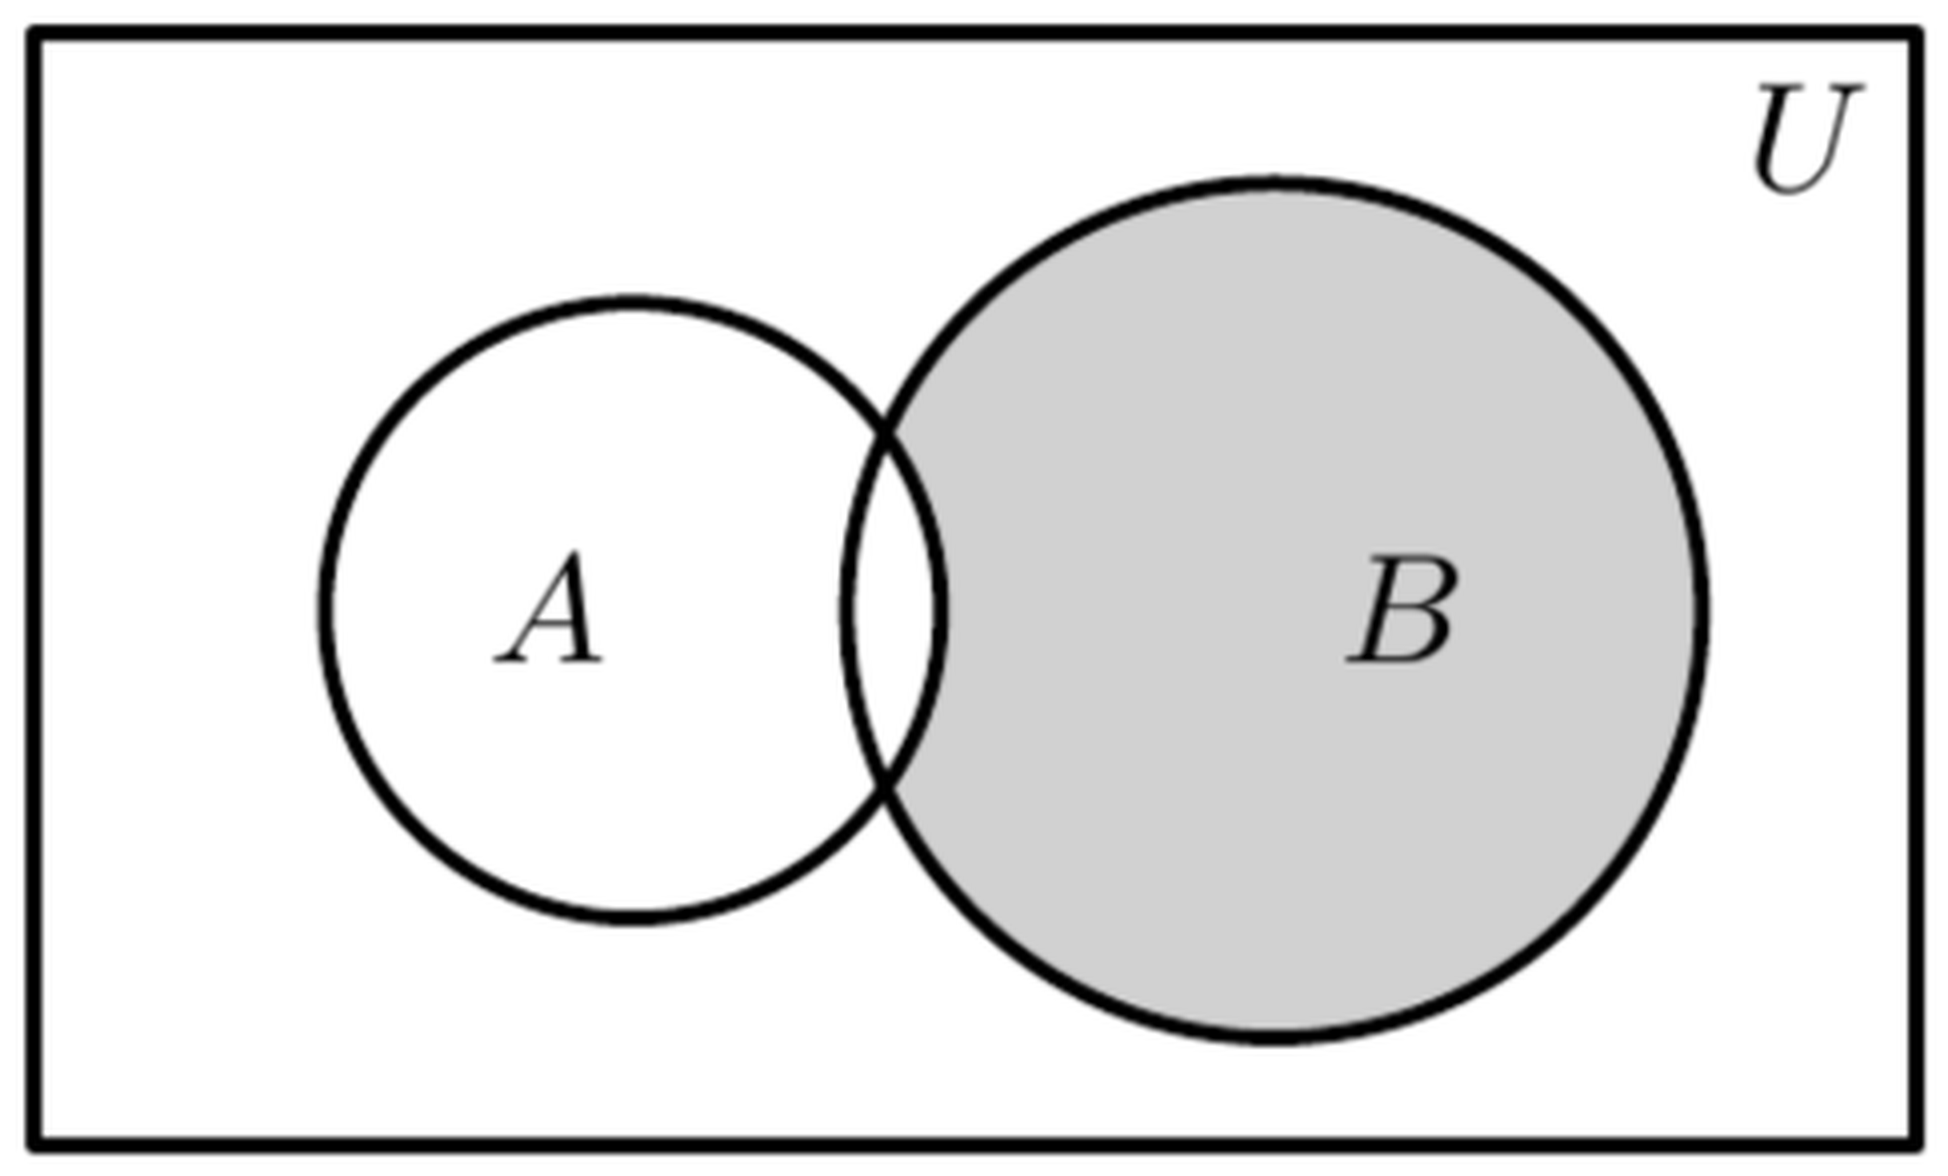
\includegraphics[width=0.38\textwidth]{figures/gao160_q4.png}
\end{center}

\ifanswer
\solbegin
\step{阴影部分表示 $B\cap\overline{A}=\{1,2\}$.}
\solend
\fi

% === Q5 === "图像"（有亻）照录；解析 1 行
\item 已知常数 $a>0$ 且 $a\ne1$，假设无论 $a$ 取何值，函数 $y=\log_a(5x-9)-4$ 的图像恒过一个定点，则这个定点的坐标为\blankline[4.4em].

\ifanswer
\solbegin
\step{$5x-9=1\Rightarrow x=2$，此时 $y=\log_a 1-4=-4$，定点为 $(2,-4)$.}
\solend
\fi

% === Q6 === 解析 2 行
\item 不等式 $(1-2x)^{\frac{3}{4}}>x^{\frac{3}{4}}$ 的解集为\blankline[4.4em].

\ifanswer
\solbegin
\step{定义域为 $\left[0,\dfrac{1}{2}\right]$，由幂函数的单调性，原不等式等价于 $1-2x>x$，}
\step{得 $0\leqslant x<\dfrac{1}{3}$，故解集为 $\left[0,\dfrac{1}{3}\right)$.}
\solend
\fi

% === Q7 === 绝对值 \lvert…\rvert；解析 2 行（跨 01—02 页）
\item 已知不等式 $\lvert x+3\rvert+\lvert x-2\rvert\geqslant 5$，当其等号成立时，$x$ 的取值范围是\blankline[4.4em].

\ifanswer
\solbegin
\step{$\lvert x+3\rvert+\lvert x-2\rvert=\lvert x+3\rvert+\lvert 2-x\rvert\geqslant\lvert(x+3)+(2-x)\rvert=5$，}
\step{等号成立当且仅当 $(x+3)(2-x)\geqslant0$，即 $x\in[-3,2]$.}
\solend
\fi

% === Q8 === 解析 4 行
\item 已知函数 $f(x)=\lvert\log_2 x\rvert$，若方程 $f(x)-t=0$ 有两个不同的实数根 $x_1,x_2$，则 $x_1+x_2$ 的取值范围是\blankline[4.4em].

\ifanswer
\solbegin
\step{方程有两个不同实根，必有 $t>0$，两根为 $2^t,2^{-t}$，}
\step{所以 $x_1+x_2=2^t+2^{-t}>2$（等号仅在 $t=0$ 时成立）.}
\step{任取 $s>2$，令 $a=\dfrac{s+\sqrt{s^2-4}}{2}>1$，取 $t=\log_2 a>0$，则 $x_1+x_2=a+\dfrac{1}{a}=s$，}
\step{所以取值范围为 $(2,+\infty)$.}
\solend
\fi

% === Q9 === 中文弯引号、\R、绝对值 \lvert…\rvert；解析 4 行
\item 已知 $a\in\R$，$b\in\R$，$p:\dfrac{1}{\lvert a\rvert}>\dfrac{1}{\lvert b\rvert}$，$q:\dfrac{1}{a}>\dfrac{1}{b}$，则 $p$ 是 $q$\blankline[4.4em]条件（用“充分非必要”、“必要非充分”、“充要”或“既非充分又非必要”填空）.

\ifanswer
\solbegin
\step{由 $p$、$q$ 中的分式有意义，$a\ne0$ 且 $b\ne0$.}
\step{当 $a=-1,b=-2$ 时，$p$ 成立而 $q$ 不成立，故 $p$ 不是 $q$ 的充分条件.}
\step{当 $a=1,b=-1$ 时，$q$ 成立而 $p$ 不成立，故 $p$ 不是 $q$ 的必要条件.}
\step{故 $p$ 是 $q$ 的充分非必要条件.}
\solend
\fi

% === Q10 === 解析 3 行；其后独立【注】按语 5 行（见头注 ② ⑯、⑤ 1）
\item 已知常数 $a>0$，函数 $y=\dfrac{2^x}{2^x+ax}$ 的图像经过点 $P\left(p,\dfrac{5}{6}\right)$、$Q\left(q,\dfrac{1}{6}\right)$，若 $2^{p+q}=3pq$，则 $a=$\blankline[4.4em].

\ifanswer
\solbegin
\step{由 $\dfrac{2^p}{2^p+ap}=\dfrac{5}{6}$ 得 $2^p=5ap$；由 $\dfrac{2^q}{2^q+aq}=\dfrac{1}{6}$ 得 $2^q=\dfrac{aq}{5}$.}
\step{$2^p>0$，$2^q>0$，$a>0$，得 $p>0$，$q>0$.}
\step{两式相乘得 $2^{p+q}=a^2pq$，又 $2^{p+q}=3pq$ 且 $pq\ne0$，故 $a^2=3$，$a=\sqrt{3}$.}
\solend
% 【注】按语（讲评版编者按，5 个印刷行，仅答案版出，不属于任何题的【解析】）
\stepm{【注】}{按原卷数据严格推敲，点 $Q$ 其实不存在：$a=\sqrt{3}$ 时 $2^q=\dfrac{\sqrt{3}}{5}q<q$；而当 $q>0$}
\step{时，取非负整数 $n$ 使 $n\leqslant q<n+1$，由 $2^{k+1}=2^k+2^k\geqslant2^k+1$ 逐次推得 $2^n\geqslant n+1$，于是}
\step{$2^q\geqslant2^n\geqslant n+1>q$，矛盾. 所以题设条件互相矛盾，严格说本题无解；$\sqrt{3}$ 是由题给关}
\step{系直接推出的值，按命题意图作为答案. 原卷数据疑似有误（同型常见题为 $P\left(p,\dfrac{6}{5}\right)$、}
\step{$Q\left(q,-\dfrac{1}{5}\right)$、$2^{p+q}=36pq$，得 $a=6$）.}% 见头注 ⑤ 1，照录未改
\fi

% === Q11 === 纳皮尔对数材料题；\Z、大数；解析 6 行
\item 17 世纪初，约翰·纳皮尔为了简化计算而发明了对数. 对数的发明是数学史上的重大事件，恩格斯曾经把笛卡尔的坐标系、纳皮尔的对数、牛顿和莱布尼兹的微积分共同称为 17 世纪的三大数学发明. 我们知道，任何一个正实数 $N$ 可以表示成 $N=a\times10^n$ ($1\leqslant a<10,n\in\Z$) 的形式，这便是科学记数法，若两边取常用对数，有 $\lg N=n+\lg a$，则可以估计 $3^{2026}$ 的最高位上的数值为\blankline[4.4em].

\ifanswer
\solbegin
\step{设 $3^{2026}=a\times10^n$ ($1\leqslant a<10,n\in\Z$)，则 $2026\lg 3=n+\lg a$.}
\step{用 $\lg 3\approx 0.4771$ 粗估，得 $2026\lg 3\approx 966.60$.}
\step{为核验误差，用 $0.47712<\lg 3<0.47713$，}
\step{得 $966.64512<2026\lg 3<966.66538$，因此 $n=966$.}
\step{于是 $\lg 4\approx 0.60206<0.64512<\lg a<0.66538<\lg 5\approx 0.69897$，}
\step{所以 $4<a<5$，最高位为 4，估算误差不影响结论.}
\solend
\fi

% === Q12 === 自定义"性质 P"；文本圈数字①②③；解析 19 行（跨 03—05 页）
\item 对于数集 $X=\{-1,x_1,x_2,x_3,\cdots,x_n\}$，其中 $0<x_1<x_2<x_3<\cdots<x_n$，$n\geqslant2$，定义点集 $Y=\{(s,t)\mid s\in X,t\in X\}$，若对于任意 $(s_1,t_1)\in Y$，存在 $(s_2,t_2)\in Y$，使得 $s_1s_2+t_1t_2=0$，则称集合 $X$ 具有性质 $P$. 则下列命题中为真命题的是\blankline[4.4em].

① $X=\{-1,1,2\}$ 具有性质 $P$；②若集合 $X$ 具有性质 $P$，则 $1\in X$；

③集合 $X$ 具有性质 $P$，若 $x_1=\dfrac{1}{2}$，则 $x_n=2$.

\ifanswer
\solbegin
\step{因为 $X=\{-1,1,2\}$，}
\step{所以 $Y=\{(-1,-1),(1,1),(2,2),(-1,1),(-1,2),(1,-1),(1,2),(2,-1),(2,1)\}$，}
\step{由集合 $X$ 具有性质 $P$ 的定义，对于任意 $(s,t)\in Y$，}
\step{若 $s>0$，$t>0$，则 $s=t$ 或 $(s,t)=(1,2)$ 或 $(s,t)=(2,1)$，}
\step{若 $s=t$，取 $s_2=-1$，$t_2=-1$，则 $ss_2+tt_2=0$；}
\step{若 $(s,t)=(1,2)$，取 $s_2=2$，$t_2=-1$，则 $ss_2+tt_2=0$；}
\step{若 $(s,t)=(2,1)$，取 $s_2=-1$，$t_2=2$，则 $ss_2+tt_2=0$；}
\step{若 $s$、$t$ 有一个为负数，则 $s=-1$ 或 $t=-1$，}
\step{若 $s=-1$，则取 $s_2=t$，$t_2=1$，则 $ss_2+tt_2=0$；}
\step{若 $t=-1$，则取 $s_2=1$，$t_2=s$，则 $ss_2+tt_2=0$；故①正确；}
\step{对于任意 $(s_1,t_1)\in Y$，存在 $(s_2,t_2)\in Y$，使得 $s_1s_2+t_1t_2=0$，}
\step{取 $(x_1,x_1)\in Y$，存在 $(x_p,x_q)$ 使得 $x_1x_p+x_1x_q=0$，所以 $x_p+x_q=0$，}
\step{不妨设 $x_p=1$，$x_q=-1$，所以若集合 $X$ 具有性质 $P$，则 $1\in X$，故②正确；}
\step{③假设 $x_n>1$，令 $s_1=\dfrac{1}{2},t_1=x_n$，则存在 $s$、$t\in X$ 使得 $\dfrac{1}{2}s+tx_n=0$，}
\step{同②得 $s$、$t$ 中必有一个数为 $-1$，}
\step{若 $s=-1$，则 $tx_n=\dfrac{1}{2}$，于是 $t=\dfrac{1}{2x_n}<\dfrac{1}{2}=x_1$，矛盾，}
\step{若 $t=-1$，则 $\dfrac{1}{2}s=x_n\cdot(-1)$，于是 $s=2x_n>x_n$，也矛盾，}% 原卷如此（与结论符号不自洽），照录未改，见头注 ⑤ 2
\step{所以 $x_n\leqslant1$，又由②得 $1\in X$，所以 $x_n\geqslant1$，所以 $x_n=1$，故③错误，}
\step{故真命题是①②.}
\solend
\fi

\end{enumerate}

% 答案版里填空解析把页排满，节标题会落到页末、与第 13 题分家（切页审计 B 类）；
% 守卫放 \bigsec 之前，连节标题一起量页高（高一157 成例）
\needvspace{7cm}
\bigsec{二、选择题}

\begin{enumerate}
\setcounter{enumi}{12}

% === Q13 === "图像"照录；解析 1 行，故选 $B$
\item 下列函数中，图像与函数 $y=3^x$ 图像关于 $y$ 轴对称的是\mbox{（\quad）}

\keepwithprev
A. $y=x^3$\qquad B. $y=\left(\dfrac{1}{3}\right)^x$\qquad C. $y=-3^x$\qquad D. $y=\log_3 x$

\ifanswer
\solbegin
\step{将 $x$ 换为 $-x$，得对称图像对应的函数为 $y=3^{-x}=\left(\dfrac{1}{3}\right)^x$，故选 $B$.}
\solend
\fi

% === Q14 === 中文弯引号；解析 2 行（跨 05 页上下），故选 $B$
\item 命题“存在 $x\in(1,+\infty)$，使得 $f(x)>0$”的否定形式为\mbox{（\quad）}

\keepwithprev
A. 不存在 $x\in(-\infty,1]$，使得 $f(x)>0$\qquad B. 对任意 $x\in(1,+\infty)$，有 $f(x)\leqslant0$

C. 对任意 $x\in(-\infty,1]$，有 $f(x)\leqslant0$\qquad D. 存在 $x\in(1,+\infty)$，使得 $f(x)\leqslant0$

\ifanswer
\solbegin
\step{将“存在”改为“对任意”，$x$ 的范围不变，并将 $f(x)>0$ 否定为 $f(x)\leqslant0$，}
\step{故选 $B$.}
\solend
\fi

% === Q15 === \R；四选项两行；解析 3 行，故选 $D$
\item 设 $a>0$，$s\in\R$. 下列各项中，能推出 $a^s>a$ 的一项是\mbox{（\quad）}

\keepwithprev
A. $a>1$，且 $s>0$\qquad B. $a>1$，且 $s<0$

C. $0<a<1$，且 $s>0$\qquad D. $0<a<1$，且 $s<0$

\ifanswer
\solbegin
\step{当 $a>1$ 时，$a^s>a\Leftrightarrow s>1$，A、B 均不能保证.}
\step{当 $0<a<1$ 时，$a^s>a\Leftrightarrow s<1$，C 不能保证，D 中 $s<0<1$，满足要求；}
\step{故选 $D$.}
\solend
\fi

% === Q16 === 题目配图（三版都出）；几何符号 \triangle ABC；解析 3 行，故选 $C$
\needvspace{8cm}
\item 数学说明的方法多种多样，其中利用图形说明就是一种重要方法. 如图所示，在等腰直角三角形 $\triangle ABC$ 中，点 $O$ 为斜边 $AB$ 的中点，点 $D$ 为斜边 $AB$ 上异于顶点的一个动点，设 $AD=a$，$BD=b$，则可用该图形能说明的不等式为\mbox{（\quad）}

\begin{center}
% Q16 等腰直角三角形 ABC 图（C/A/O/D/B 标注）取 05 页右下，去粉色水印、去色、3× LANCZOS 放大；三版都出
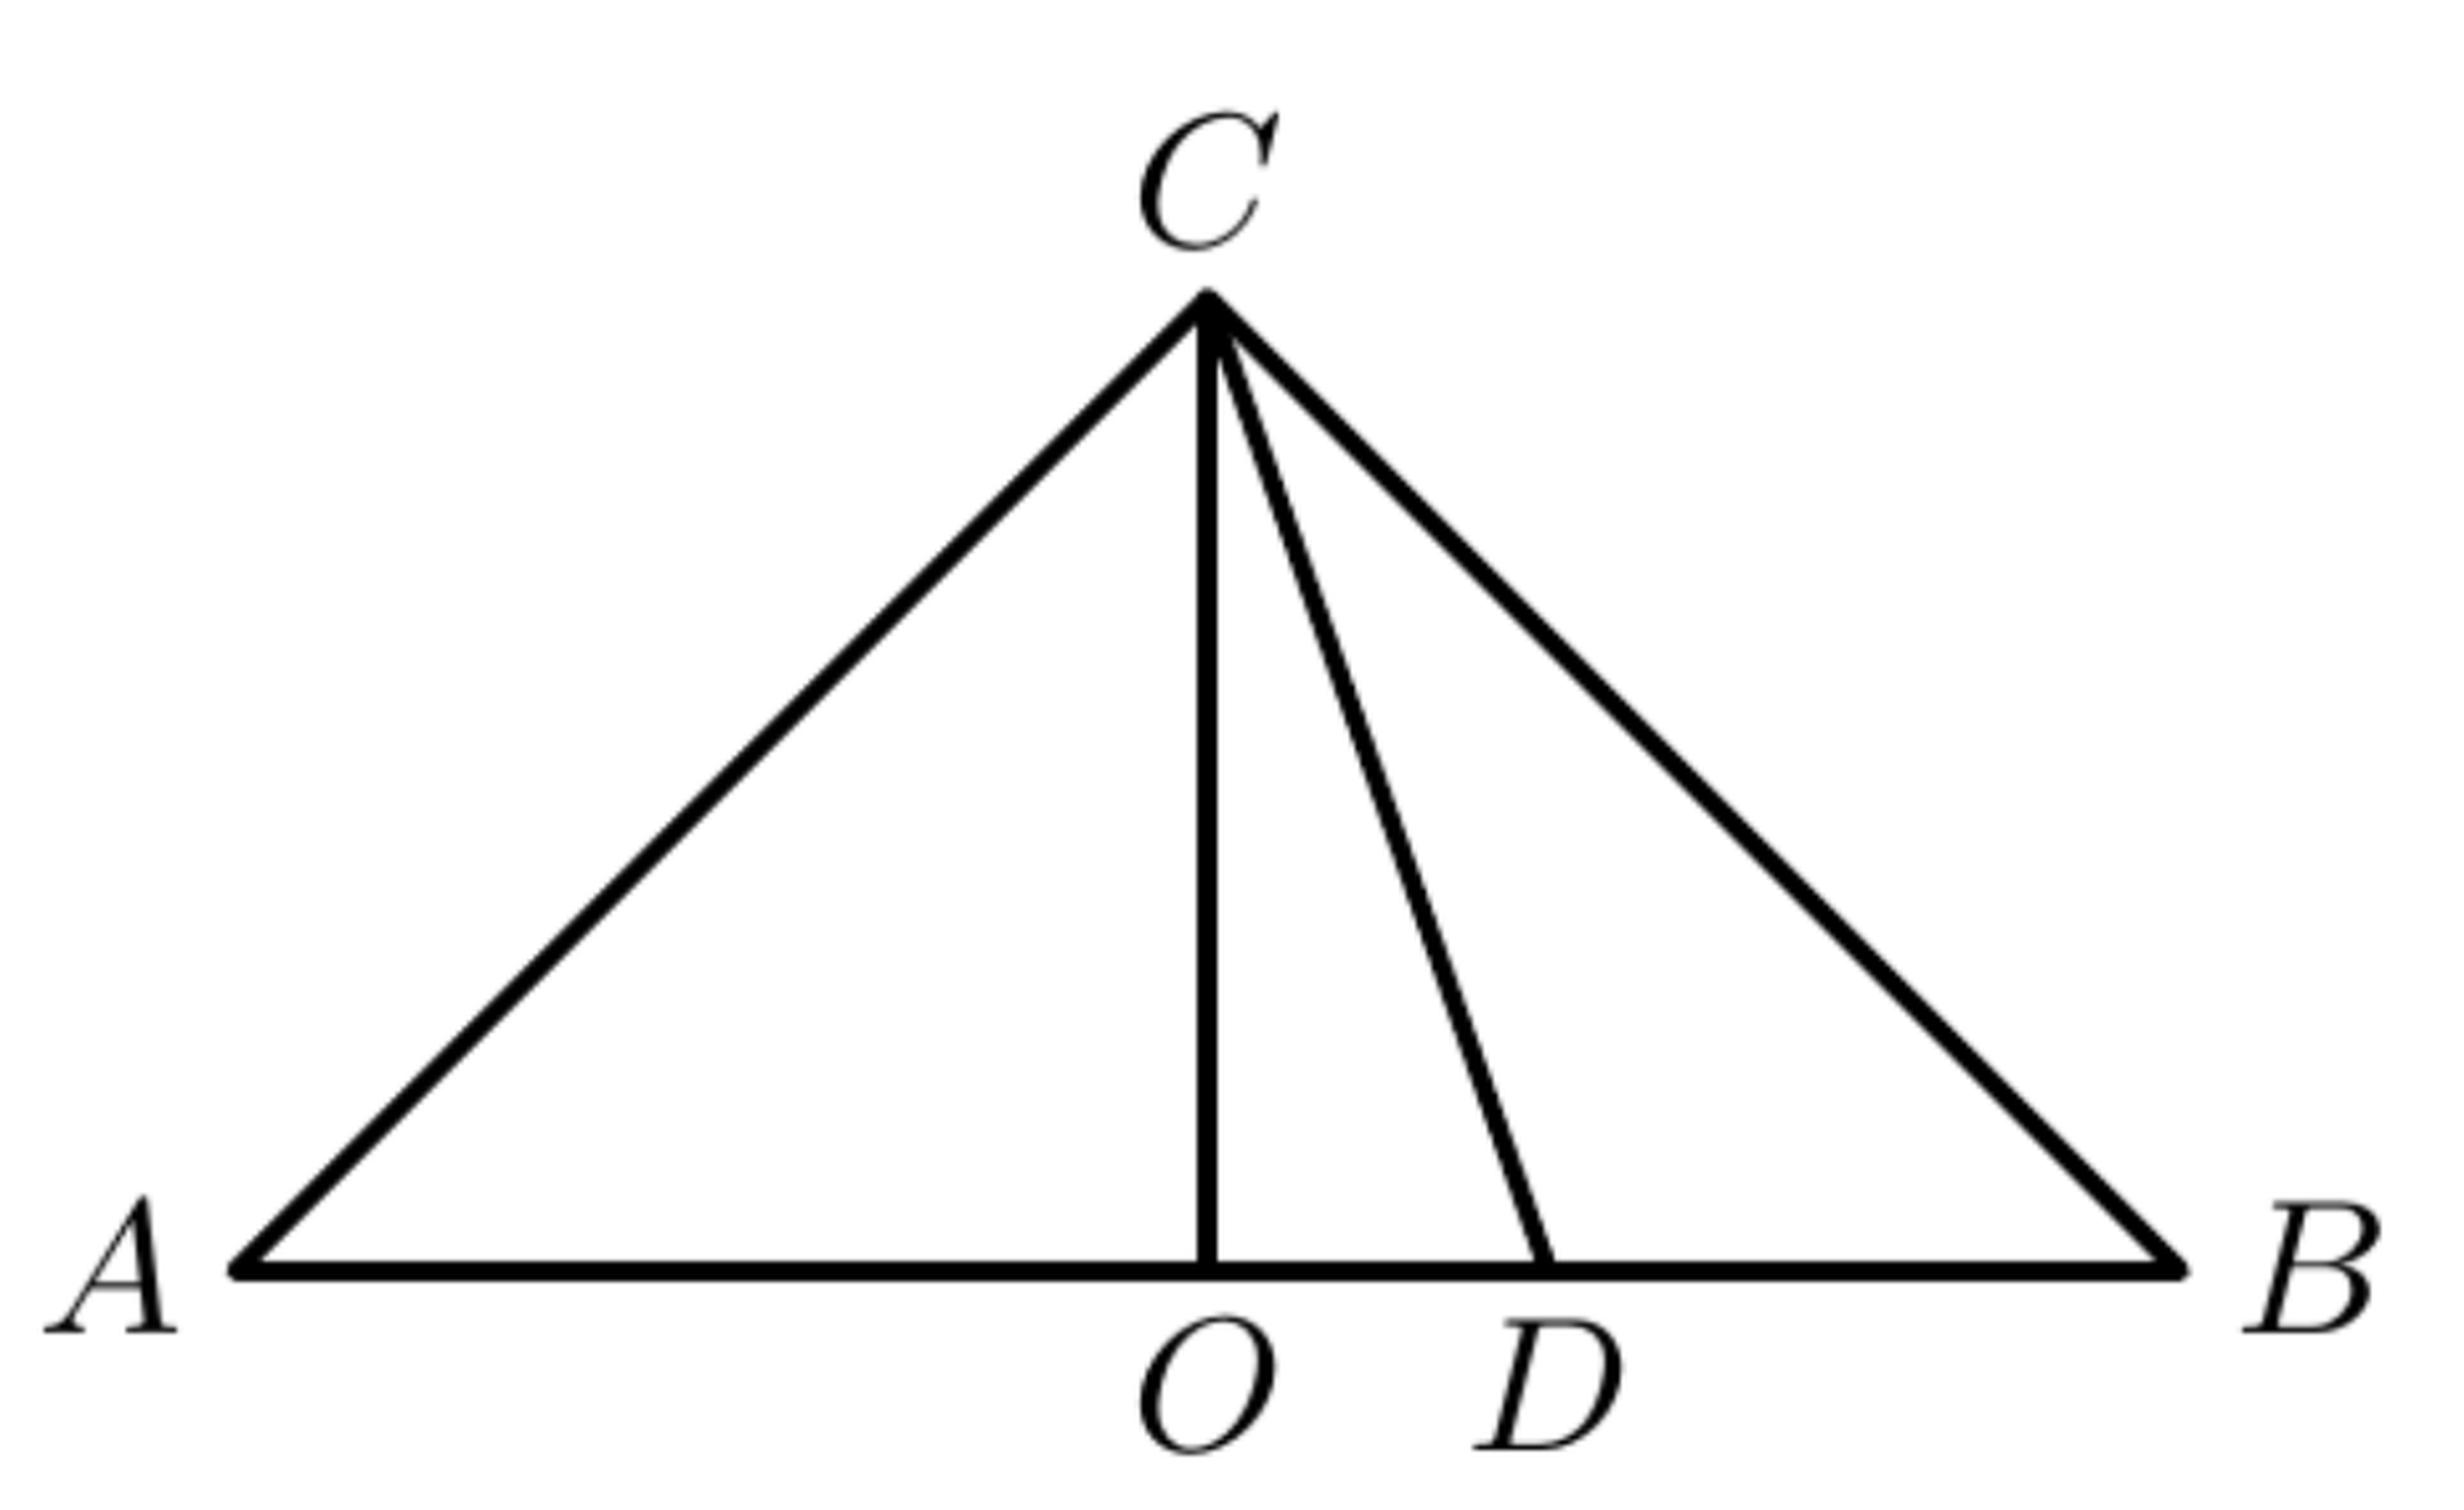
\includegraphics[width=0.34\textwidth]{figures/gao160_q16.png}
\end{center}

\keepwithprev
A. $\dfrac{a+b}{2}\geqslant\sqrt{ab}$ ($a>0,b>0$)\qquad B. $a^2+b^2\geqslant2\sqrt{ab}$ ($a>0,b>0$)

C. $\dfrac{a+b}{2}\leqslant\sqrt{\dfrac{a^2+b^2}{2}}$ ($a>0,b>0$)\qquad D. $\dfrac{2ab}{a+b}\leqslant\sqrt{ab}$ ($a>0,b>0$)

\ifanswer
\solbegin
\step{$CO=AO=\dfrac{a+b}{2},OD=\left\lvert a-\dfrac{a+b}{2}\right\rvert=\dfrac{\lvert a-b\rvert}{2}$，}
\step{$CD=\sqrt{CO^2+OD^2}=\sqrt{\dfrac{a^2+b^2}{2}}\geqslant CO=\dfrac{a+b}{2}$，}
\step{等号当且仅当 $a=b$ 时成立，故选 $C$.}
\solend
\fi

\end{enumerate}

\bigsec{三、解答题}

\begin{enumerate}
\setcounter{enumi}{16}

% === Q17 === cases 块算一行；判别式印等腰偏高三角 \Delta；解析 7 行
\item 已知幂函数 $f(x)=(m^2-2m-2)x^{m-1}$ 在 $(0,+\infty)$ 上是严格增函数.

(1) 求 $m$ 的值；

(2) 若关于 $x$ 的方程 $f(x)=(t+1)x-t^2$ 有两个不相等的正实根，求实数 $t$ 的取值范围.

\ifanswer
\solbegin
\step{(1) 幂函数的系数为 1，因此 $m^2-2m-2=1\Leftrightarrow(m-3)(m+1)=0$，}
\step{解得 $m=3$ 或 $m=-1$.}
\step{由 $f(x)$ 在 $(0,+\infty)$ 上严格递增，得 $m-1>0$，所以 $m=3$，}
\step{此时 $f(x)=x^2$.}
\step{(2) 原方程化为 $x^2-(t+1)x+t^2=0$，}
\step{方程有两个不相等的正实根，则 $\begin{cases}\Delta=(t+1)^2-4t^2=(1-t)(3t+1)>0\\t+1>0\\t^2>0\end{cases}$，}% 判别式原卷印等腰偏高三角 \Delta，照录
\step{得 $t\in\left(-\dfrac{1}{3},0\right)\cup(0,1)$.}
\solend
\fi

% === Q18 === 补集上划线 \overline{A}、\subseteq 带下划线、\varnothing；解析 8 行
\item 已知集合 $A=\{x\mid\lvert x-a\rvert<a-3\}$，$B=\left\{x\mid\dfrac{x+1}{x-2}\geqslant2\right\}$.

(1) 若 $a=5$，求 $\overline{A}\cap B$；

(2) 若 $A\cap B=A$，求实数 $a$ 的取值范围.

\ifanswer
\solbegin
\step{(1) $\dfrac{x+1}{x-2}\geqslant2\Leftrightarrow\dfrac{5-x}{x-2}\geqslant0\Leftrightarrow2<x\leqslant5,B=(2,5]$，}
\step{当 $a=5$ 时，$A=\{x\mid\lvert x-5\rvert<2\}=(3,7)$，于是 $\overline{A}=(-\infty,3]\cup[7,+\infty)$，}
\step{因此 $\overline{A}\cap B=(2,3]$.}
\step{(2) $A\cap B=A$ 等价于 $A\subseteq B$.}
\step{当 $a\leqslant3$ 时，$a-3\leqslant0$，$A=\varnothing$，满足条件.}
\step{当 $a>3$ 时，$\lvert x-a\rvert<a-3\Leftrightarrow3<x<2a-3,A=(3,2a-3)$，}
\step{此时 $A\subseteq B=(2,5]$ 等价于 $2a-3\leqslant5$，即 $a\leqslant4$，结合 $a>3$ 得 $3<a\leqslant4$.}
\step{合并两种情形，实数 $a$ 的取值范围为 $(-\infty,4]$.}
\solend
\fi

% === Q19 === 数据表 tabular 重排（高一130 成例）；cases 块算一行；解析 6 行
\item 作为我国最高水平的综合性运动会，全运会汇聚了国内顶尖体育健儿，某代表队从第 8 届全运会开始登上赛场，且参赛运动员人数逐年递增. 设 $t$ 为该代表队参赛后经过的届数，即第 8 届为 $t=0$，第 9 届为 $t=1$，以此类推. 经过 $t$ 届，运动员人数为 $y$ 人，具体数据如下：

\begin{center}
\begin{tabular}{cccccc}
$t$ & 0 & 1 & 2 & 3 & 4 \\
\hline
届数 & 8 & 9 & 10 & 11 & 12 \\
运动员人数（$y$ 人） & 4 & 11 & 25 & 53 & 109
\end{tabular}
\end{center}

(1) 现有以下两种函数模型：① $y=a\cdot b^t+c$ ($a>0,b>1$)；② $y=\log_a(t+b)+c$ ($b>0,a>1$). 请根据上表中运动员人数的增长规律，选出你认为符合的函数模型（不用说明理由），并利用表中前 3 组数据求出相应的函数解析式；

(2) 若参赛运动员人数按照 (1) 中求得的模型继续增长，在第几届全运会时，该代表队运动员人数将会首次超过 1000 人？

\ifanswer
\solbegin
\step{(1) 选模型①，将前 3 组数据代入，得 $\begin{cases}a+c=4\\ab+c=11\\ab^2+c=25\end{cases}$，}% 原卷印"选模型①"（圈数字①），OCR 误作"四"，照录①，见头注 ⑤ 3
\step{相邻两式相减，得 $a(b-1)=7$，$ab(b-1)=14$，}
\step{两式相除得 $b=2$，进而 $a=7$，$c=-3$，所求函数解析式为 $y=7\cdot2^t-3$.}
\step{(2) $y=7\cdot2^t-3$ 随 $t$ 的增大而增大，且 $t=7$ 时，$y=893<1000$；}
\step{$t=8$ 时，$y=1789>1000$，}
\step{$t$ 为非负整数，首次超过 1000 人时 $t=8$，对应第 $8+8=16$ 届全运会.}
\solend
\fi

% === Q20 === 解析 12 行（跨 08—09 页）
\item 已知函数 $f(x)=\log_a(a-a^x)$.

(1) 求该函数的定义域；

(2) 若 $a>1$，试判断关于 $x$ 的方程 $f(x)=2$ 是否有实数解，并说明理由；

(3) 若当 $x\in(-\infty,0]$ 时，关于 $x$ 的不等式 $f(x)\geqslant-1$ 恒成立，求实数 $a$ 的取值范围.

\ifanswer
\solbegin
\step{(1) 对数的底数须满足 $a>0$ 且 $a\ne1$，真数须满足 $a-a^x>0$，即 $a^x<a^1$.}% 原卷印 $a^1$，照录未化简，见头注 ⑤ 4
\step{当 $a>1$ 时，$x<1$，定义域为 $(-\infty,1)$.}
\step{当 $0<a<1$ 时，$x>1$，定义域为 $(1,+\infty)$.}
\step{(2) 当 $a>1$ 时，若 $f(x)=2$，则 $a-a^x=a^2\Rightarrow a^x=a(1-a)<0$，}
\step{这与 $a^x>0$ 矛盾，因此方程无实数解.}
\step{(3) 不等式在 $(-\infty,0]$ 上恒成立，须先保证该区间包含于函数的定义域，}
\step{由 (1) 得 $a>1$.}
\step{当 $x\leqslant0$ 时，$0<a^x\leqslant1$，所以 $a-a^x\geqslant a-1>0$.}
\step{由对数函数的单调性，$f(x)=\log_a(a-a^x)\geqslant\log_a(a-1)=f(0)$，}
\step{等号当且仅当 $x=0$ 时成立，}
\step{因此所求条件等价于 $\log_a(a-1)\geqslant-1\Leftrightarrow a-1\geqslant\dfrac{1}{a}\Leftrightarrow a^2-a-1\geqslant0$，}
\step{结合 $a>1$，得 $a\in\left[\dfrac{1+\sqrt{5}}{2},+\infty\right)$.}
\solend
\fi

% === Q21 === "和积平衡集"定义证明题；\N；解析 18 行（跨 09—10 页）
\item 已知有限集 $A=\{a_1,a_2,\cdots,a_n\}$ ($n\geqslant2,n\in\N$)，如果 $A$ 中元素 $a_i$ ($i=1,2,3,\cdots,n$) 满足 $a_1+a_2+a_3+\cdots+a_n=a_1\times a_2\times\cdots\times a_n$，就称 $A$ 为“和积平衡集”.

(1) 分别判断集合 $A=\{1,2,3,4\}$，$B=\{4+2\sqrt{2},4-2\sqrt{2}\}$ 是否为“和积平衡集”；

(2) 已知 $a_1$、$a_2$ 是两个不同的正数，且 $\{a_1,a_2\}$ 是“和积平衡集”，请用反证法证明：$a_1$、$a_2$ 至少有一个大于 2；

(3) 若 $a_i\geqslant1$，且 $a_i\in\N$，求所有符合条件的“和积平衡集”.

\ifanswer
\solbegin
\step{(1) 因为 $1+2+3+4=10\ne24=1\times2\times3\times4$，所以 $A$ 不是“和积平衡集”.}
\step{因为 $(4+2\sqrt{2})+(4-2\sqrt{2})=8=(4+2\sqrt{2})(4-2\sqrt{2})$，}
\step{所以 $B$ 是“和积平衡集”.}
\step{(2) 假设 $a_1$、$a_2$ 都不大于 2，则 $\dfrac{1}{a_1}\geqslant\dfrac{1}{2},\dfrac{1}{a_2}\geqslant\dfrac{1}{2}$，}
\step{由于 $a_1\ne a_2$，上述两个不等式至少有一个严格成立.}
\step{而 $a_1+a_2=a_1a_2$，两边除以 $a_1a_2>0$，得 $1=\dfrac{1}{a_1}+\dfrac{1}{a_2}>\dfrac{1}{2}+\dfrac{1}{2}=1$，矛盾，}
\step{所以 $a_1$、$a_2$ 至少有一个大于 2.}
\step{(3) 不妨设 $a_1<a_2<\cdots<a_n$，由各元素均为正整数，得 $a_i\geqslant i$.}
\step{若 $n\geqslant4$，因其余因子均不小于 1，}
\step{有 $a_1a_2\cdots a_n\geqslant a_2a_{n-1}a_n\geqslant2(n-1)a_n>na_n>a_1+a_2+\cdots+a_n$，}
\step{与和积平衡条件矛盾，因此只需讨论 $n=2,3$.}
\step{当 $n=2$ 时，$a_1+a_2=a_1a_2\Leftrightarrow(a_1-1)(a_2-1)=1$，}
\step{两个因子均为非负整数，只能有 $a_1=a_2=2$，与元素互不相同矛盾.}
\step{当 $n=3$ 时，若 $a_1\geqslant2$，则 $a_2\geqslant3$，从而 $a_1a_2a_3\geqslant6a_3>3a_3>a_1+a_2+a_3$，}
\step{矛盾，因此 $a_1=1$.}
\step{此时 $1+a_2+a_3=a_2a_3\Leftrightarrow(a_2-1)(a_3-1)=2$，}
\step{由 $1\leqslant a_2-1<a_3-1$，得 $a_2-1=1$、$a_3-1=2$，即 $a_2=2$、$a_3=3$.}
\step{检验 $1+2+3=1\times2\times3=6$，所求集合为 $\{1,2,3\}$.}
\solend
\fi

\end{enumerate}

\end{document}
"
%
% ① 原始材料：微信公众号"魔都数学加油站"文章，连载"27学年高一160"，原卷卷面标题
% "2026-2027 年奉贤中学高一上期中"（卷面未印副标题、未印连载号）。
% 正文为 10 张 PNG 页（01/04/10 为 2560×3620，02/03/05/06/07/08/09 为
% 4762×6735，同一篇各页分辨率混排，逐页按各自分辨率裁图核对）。
% 体例：讲评版——填空 3—12（10 题）、选择 13—16（4 题）、解答 17—21（5 题），
% 共 19 题，自第 3 题起编（1、2 未印在本篇）；19 题逐题印【解析】，无只印【答案】
% 的题；四道选择题答案在解析末句"故选 $B$/$B$/$D$/$C$"，题干括号
% \mbox{（\quad）} 留空、不另提 \ans{}。题目、答案、解析均据原图转录；卷面粉红色
% 水印"魔都数学加油站"及公众号页脚未录入。
% 全卷插图清单（逐页通读 10 页确认）：2 幅，均为题目配图、三版都出——
%   · Q4 韦恩图（01 页右侧：矩形全集 U、两圆 A/B、阴影部分 B∩上划线 A、
%     标注 U/A/B），裁 figures/gao160_q4.png；
%   · Q16 等腰直角三角形 ABC 图（05 页右下：C 顶点、A/O/D/B 共线底边、
%     CO 与 CD 两条线段），裁 figures/gao160_q16.png；
%   两图均取原卷截图 3—4× LANCZOS 放大、去粉色水印、转灰度、autocontrast；
%   Q4 图左侧题干残字"示"、Q16 图左侧题干残字均已裁白。
%   Q19 有一张 3 行数据表（t／届数／运动员人数（y 人），t=0..4），按全稿
%   成例（高一130）用 tabular 重排，不做成 png；其余各页无题目配图、
%   无解析内配图、无其它表格、无"如图"处。
%
% 卷首标题：原卷印作"2026-2027 年奉贤中学高一上期中"，年份区间按全稿惯例排 en dash；
% 原卷卷面未印副标题，本稿按同期中卷知识模块口径补出"集合与常用逻辑用语、不等式、函数"。
%
% ② 与原卷的排版差异／照录项清单：
%   ① 原文从第 3 题起，本稿保留原题号；共 19 题三节，解答题 5 题到 21；
%      三节各自一个 enumerate + \setcounter{enumi}{2}/{12}/{16}（不贯穿），
%      用 \examtitlest[3] 起手；
%   ② 混合体例说明：19 题全印【解析】、用 \solbegin…\solend，无只印【答案】
%      或答案印括号内的题；四道选择题答案在解析末句"故选 $B$/$B$/$D$/$C$"
%      （逐个放大复核）、括号 \mbox{（\quad）} 留空、不另提 \ans{}；答案版
%      【答案】/【解析】标记数 = 19 = 全卷题数（0 个 \ans ＋ 19 个 \solbegin）；
%   ③ 原卷卷面未印副标题，本稿按知识模块口径补出；
%   ④ 原卷填空横线按全稿惯例排 \blankline[4.4em]；选择题括号排 \mbox{（\quad）}、
%      四道选择题的选项段前按惯例各加 \keepwithprev；解答题不留作答区、不加
%      \anspace（原卷为讲评版，109—113 起全稿不用 \anspace）；
%   ⑤ 数集归一：Q4"$U=\Z$"、Q9"$a\in\R$，$b\in\R$"、Q11"$n\in\Z$"、
%      Q15"$s\in\R$"、Q21"$n\in\N$""$a_i\in\N$"原卷印正体粗体 Z/R/N，
%      按全稿惯例归一 \Z／\R／\N；集合描述竖线排 \mid（Q3、Q4、Q12、
%      Q18、Q21）；空集 \varnothing（Q18 解析 (2)）；补集照原卷上划线排
%      \overline{A}（Q4 解析、Q18 (1) 题干与解析）；子集符号 Q18 两处
%      "$A\subseteq B$"印带下划线 ⊆、照录 \subseteq；
%   ⑥ 绝对值排 \lvert…\rvert（Q7、Q8 题干与解析、Q9 题干、Q16 解析、
%      Q18 题干与解析），Q16 解析的 \left\lvert…\right\rvert 与 \lvert…\rvert
%      均在同一 $…$ 组内配对平衡；
%   ⑦ 判别式两形混用逐处照录不统一（放大逐处确认）：Q3 解析
%      "$\triangle=1^2-4a\times\frac{1}{4}=0$"原卷印扁等边三角、照录
%      \triangle；Q17 解析 cases 块"$\Delta=(t+1)^2-4t^2=(1-t)(3t+1)>0$"
%      原卷印等腰偏高三角、照录 \Delta；Q16 题干几何符号"$\triangle ABC$"
%      按全稿几何三角形记号惯例归一 \triangle（参照 高一150／132 成例）；
%   ⑧ 不等号按全稿惯例排 \leqslant／\geqslant；中文弯引号照录：Q9 题干
%      "充分非必要""必要非充分""充要""既非充分又非必要"、Q14 题干
%      "存在 $x\in(1,+\infty)$，使得 $f(x)>0$"与解析"存在""对任意"、
%      Q21 题干与解析多处"和积平衡集"；注释里一律 ASCII 引号；
%   ⑨ 文本圈数字逐处照录：Q12 题干①②③、Q12 解析"故①正确""同②得"
%      "故②正确""③假设""故③错误""故真命题是①②"、Q19 题干①②与解析
%      "选模型①"，均为印刷圈数字（非 \textcircled、非数学模式）；
%   ⑩ 半角逗号在数学组之间是全稿惯例、非笔误，逐处照录（Q8"$2^t,2^{-t}$"、
%      Q9"$a=-1,b=-2$""$a=1,b=-1$"、Q11"$1\leqslant a<10,n\in\Z$"、
%      Q12"$s_1=\frac{1}{2},t_1=x_n$"、Q16 选项"$a>0,b>0$"与解析
%      "$CO=AO=\frac{a+b}{2},OD=...$"、Q18"$2<x\leqslant5,B=(2,5]$"
%      "$3<x<2a-3,A=(3,2a-3)$"、Q21"$n=2,3$"等）；行中全角逗号／顿号
%      照录（Q15 选项"$a>1$，且 $s>0$"、Q12 解析"$s$、$t$"、Q21 解析
%      "$a_1$、$a_2$"），顿号一律移出数学模式；
%   ⑪ "图像／图象"逐处照录：本卷 Q5"的图像恒过一个定点"、Q10"的图像经过点"、
%      Q13 题干两处"图像"与解析"对称图像对应的函数"均印"图像"（有亻）；
%      Q16 印"图形"（利用图形说明、该图形能说明），无"图象"用例；
%   ⑫ 复杂式照录别简化：Q3 $ax^2+x+\frac14=0$、Q5 $y=\log_a(5x-9)-4$、
%      Q6 $(1-2x)^{\frac34}>x^{\frac34}$ 与 $\left[0,\frac12\right]$、
%      Q8 $\frac{s+\sqrt{s^2-4}}{2}$、Q10 $y=\frac{2^x}{2^x+ax}$ 与
%      $\frac{2^p}{2^p+ap}=\frac56$、$\frac{2^q}{2^q+aq}=\frac16$、
%      Q11 $N=a\times10^n$ 与 $3^{2026}$、$2026\lg3\approx966.60$、
%      $966.64512<2026\lg3<966.66538$、Q12 $Y=\{(s,t)\mid s\in X,t\in X\}$
%      与 $\frac12 s+tx_n=0$、Q16 $\sqrt{\frac{a^2+b^2}{2}}$、
%      Q17 $x^2-(t+1)x+t^2=0$ 与 $\left(-\frac13,0\right)\cup(0,1)$、
%      Q18 $\frac{5-x}{x-2}\geqslant0$、Q19 $y=a\cdot b^t+c$ 与
%      $y=\log_a(t+b)+c$、$y=7\cdot2^t-3$、Q20 $f(x)=\log_a(a-a^x)$
%      与 $a^2-a-1\geqslant0$、$\left[\frac{1+\sqrt5}{2},+\infty\right)$、
%      Q21 $4+2\sqrt2$ 与 $(a_2-1)(a_3-1)=2$ 等；
%   ⑬ 子题标号 (1)(2)(3) 按全稿惯例排半角括号；行末／行中句点按全稿惯例
%      排 ASCII `.`（不是全角「．」）；cases 块整体算一个印刷行
%      （Q17 解析、Q19 解析 (1)）；
%   ⑭ 配图：Q4／Q16 题目配图（三版都出）放 \item 内题干之后 \begin{center}，
%      各用 \needvspace{8cm} 守卫把整块推走，**守卫放在 \item 之前**
%      （见 高一153 Q11/Q19 成例与切页审计 B 类坑）；
%   ⑮ 一条 \step = 原卷解析的一个印刷行；跨上下半页的重叠行只算一次
%      （Q4 解析、Q9 解析首行、Q11 解析首行、Q12 解析"若 $s=-1$…"一行、
%      Q18 解析"此时 $A\subseteq B=(2,5]$…"一行、Q20 (2) 题干、
%      Q21 解析"由 $1\leqslant a_2-1<a_3-1$…"一行）；原卷折行别合并；
%   ⑯ Q10 之后另有一整块【注】按语（03 页上半，5 个印刷行），是讲评版作者对
%      原卷数据自相矛盾的加注、不属于任何题的【解析】。本稿按 高一53
%      "注：…"成例放 Q10 的 \solend 之后、Q10 的 \fi 收尾之前：
%      **整块只保留 Q10 那一层外层 \ifanswer**（那个 \fi 就是 Q10 的收尾），
%      块内 \stepm{【注】}{首行} ＋ 4 条 \step 各自自带内层 \ifanswer…\fi
%      （\step／\stepm 宏内自带，源码里不手动再包一层 \ifanswer，
%      否则 题目溯源.py 的 strip_answers 非贪婪正则会错切）；
%      \stepm 第一参数直接用「【注】」作标签，与全稿 \ans 的【答案】、
%      \solbegin 的【解析】同性质，未加粗以外不另加任何样式；
%      5 行仅答案版出、不新增 \item、不影响溯源，头注 ③ 单列登记、
%      不计入 19 题逐题 \step 账；\stepm 把【注】排成加粗着色标签
%      （原卷为黑色加粗），此一处着色差异在此登记；
%   ⑰ 原卷用字照录：Q11"约翰·纳皮尔""莱布尼兹"（原卷作"兹"，非通行"茨"）、
%      "17 世纪的三大数学发明"；Q16"数学说明的方法""点 $D$ 为斜边 $AB$ 上
%      异于顶点的一个动点"；Q19"登上赛场""以此类推"；
%
% ③ 行数复核：一条 \step = 原卷解析的一个印刷行，cases 块作一个印刷行计。
%   逐题数（逐页核对定稿）：Q3：5；Q4：1；Q5：1；Q6：2；Q7：2；Q8：4；
%   Q9：4；Q10：3；Q11：6；Q12：19；Q13：1；Q14：2；Q15：3；Q16：3；
%   Q17：7；Q18：8；Q19：6；Q20：12；Q21：18。
%   合计 107 条 \step（19 题逐题印刷行账），与原卷逐题印刷行相等。
%   **本卷源码 \step 总数 = 19 题逐题合计 107 ＋ Q10 后独立【注】块 5 行
%   = 112 行**（其中 \step 111 条、\stepm 1 条；\stepm 与 4 条 \step 合为
%   【注】块 5 印刷行）。该 5 行不计入「逐题印刷行」账，也不是任何题的
%   【解析】，而是讲评版编者按语；主会话核验脚本按全文统计 \step 时总数会
%   较逐题账多 5，已与主会话对齐、属已知预期而非错误。
%   全卷 19 题均设 \solbegin…\solend，答案版【答案】/【解析】标记数
%   = 19 = 全卷题数。
%
% ④ 页码分布（供回原图复核）：
%   卷首标题＋"一、填空题"＋Q3 题干＋解析 5 行＋Q4 题干＋韦恩图＋解析
%   1 行＋Q5 题干首行在 01 页上半；Q4 解析（重叠）＋Q5 题干续＋解析 1 行＋
%   Q6 题干＋解析 2 行＋Q7 题干＋解析首行在 01 页下半；Q7 解析末行＋
%   Q8 题干＋解析 4 行＋Q9 题干＋解析首行在 02 页上半；Q9 解析（重叠首行）
%   ＋余 3 行＋Q10 题干＋解析 3 行在 02 页下半；【注】按语 5 行＋Q11 题干＋
%   解析首行在 03 页上半；Q11 解析（重叠首行）＋余 5 行＋Q12 题干＋①②
%   在 03 页下半；Q12 ③＋解析前 9 行在 04 页上半；Q12 解析（重叠 2 行）
%   ＋余 8 行在 04 页下半；Q12 解析末 2 行＋"二、选择题"＋Q13 题干＋选项＋
%   解析 1 行＋Q14 题干＋选项＋解析首行在 05 页上半；Q14 解析末行＋
%   Q15 题干＋选项＋解析 3 行＋Q16 题干＋三角形图在 05 页下半；
%   Q16 选项＋解析 3 行＋"三、解答题"＋Q17 题干＋两问在 06 页上半；
%   Q17 解析 7 行在 06 页下半；Q18 题干＋两问＋解析前 7 行＋Q19 题干首行
%   在 07 页上半；Q18 解析末行（重叠）＋Q19 题干＋表格＋两问在 07 页下半；
%   Q19 解析 6 行＋Q20 题干＋(1)(2) 在 08 页上半；Q20 (2)(3) 题干（重叠）
%   ＋解析 8 行在 08 页下半；Q20 解析末 4 行＋Q21 题干＋(1)(2) 在 09 页
%   上半；Q21 (3)＋解析前 7 行在 09 页下半；Q21 解析 (3) 余 10 行在 10 页
%   上半；Q21 末行（重叠）＋"检验 $1+2+3=1\times2\times3=6$，所求集合为
%   $\{1,2,3\}$."在 10 页下半（此后仅水印、无正文）。本稿按题连排，
%   不丢行、不并折行；全卷末题为第 21 题，无附加题节。
%
% ⑤ 存疑照录（放大原图确认，照录未改、正文对应处另有 % 注）：
%   1. Q10【注】按语：讲评版作者据 $a=\sqrt3$ 时 $2^q=\frac{\sqrt3}{5}q<q$
%      与 $2^n\geqslant n+1$ 推出点 $Q$ 不存在、"严格说本题无解"，并注明
%      "原卷数据疑似有误（同型常见题为 $P(p,\frac65)$、$Q(q,-\frac15)$、
%      $2^{p+q}=36pq$，得 $a=6$）"；本稿照录全块、未删未改（见 ② ⑯）。
%   2. Q12 解析 (3) 末段"若 $t=-1$，则 $\frac{1}{2}s=x_n\cdot(-1)$，
%      于是 $s=2x_n>x_n$，也矛盾，"中，等式右端与紧随的结论符号不自洽
%      （按题意应为 $\frac12 s=x_n$ 或 $-\frac12 s=x_n\cdot(-1)$），逐页
%      放大 04 页确认原卷即如此印、无漏看的负号，照录未改，建议主会话
%      回 04 页再放大复核一次；
%   3. Q19 解析 (1) 印"选模型①"（圈数字①，题干只有①②两种模型）；
%      OCR 误作"选模型四"，放大 08 页确认是①、照录①；
%   4. Q20 解析 (1)"即 $a^x<a^1$"末项原卷印 $a^1$（非 $a$），照录未化简；
%   5. Q11 题干"莱布尼兹"原卷作"兹"（非通行"茨"）、"约翰·纳皮尔"用
%      间隔号·，均照录未改；
%   6. Q9 题干"则 $p$ 是 $q$___条件"与解析"故 $p$ 是 $q$ 的充分非必要条件"
%      句式略异，均照录；
%   7. Q19 解析 (1) 用"前 3 组数据"、题干表格列到 $t=4$，照录未补。
%
\documentclass[a4paper,11pt]{article}
\usepackage{common}

\begin{document}

\examtitlest[3]{2026--2027 年奉贤中学高一上期中}{集合与常用逻辑用语、不等式、函数}

\bigsec{一、填空题}

\begin{enumerate}
\setcounter{enumi}{2}

% === Q3 === 解析 5 行；判别式印扁等边三角 \triangle
\item 若集合 $A=\{x\mid ax^2+x+\dfrac{1}{4}=0\}$ 有且仅有两个子集，则实数 $a=$\blankline[4.4em].

\ifanswer
\solbegin
\step{若集合 $A=\{x\mid ax^2+x+\dfrac{1}{4}=0\}$ 有且仅有两个子集，}
\step{所以方程 $ax^2+x+\dfrac{1}{4}=0$ 只有一个实数根，}
\step{当 $a=0$ 时，方程化为 $x+\dfrac{1}{4}=0$，解得 $x=-\dfrac{1}{4}$，符合题意，}
\step{当 $a\ne0$ 时，则 $\triangle=1^2-4a\times\dfrac{1}{4}=0$，解得 $a=1$，}% 判别式原卷印扁等边三角 \triangle，照录
\step{综上所述，实数 $a=0$ 或 1.}
\solend
\fi

% === Q4 === 题目配图（三版都出）；\needvspace 守卫放 \item 之前；补集上划线 \overline{A}；解析 1 行
\needvspace{8cm}
\item 设全集 $U=\Z$，集合 $A=\{x\mid -3<x<1\}$，$B=\{-1,0,1,2\}$，用列举法表示图中阴影部分为\blankline[4.4em].

\begin{center}
% Q4 韦恩图（全集 U、A/B 两圆、阴影 B∩上划线 A）取 01 页右侧，去粉色水印、去色、4× LANCZOS 放大；三版都出
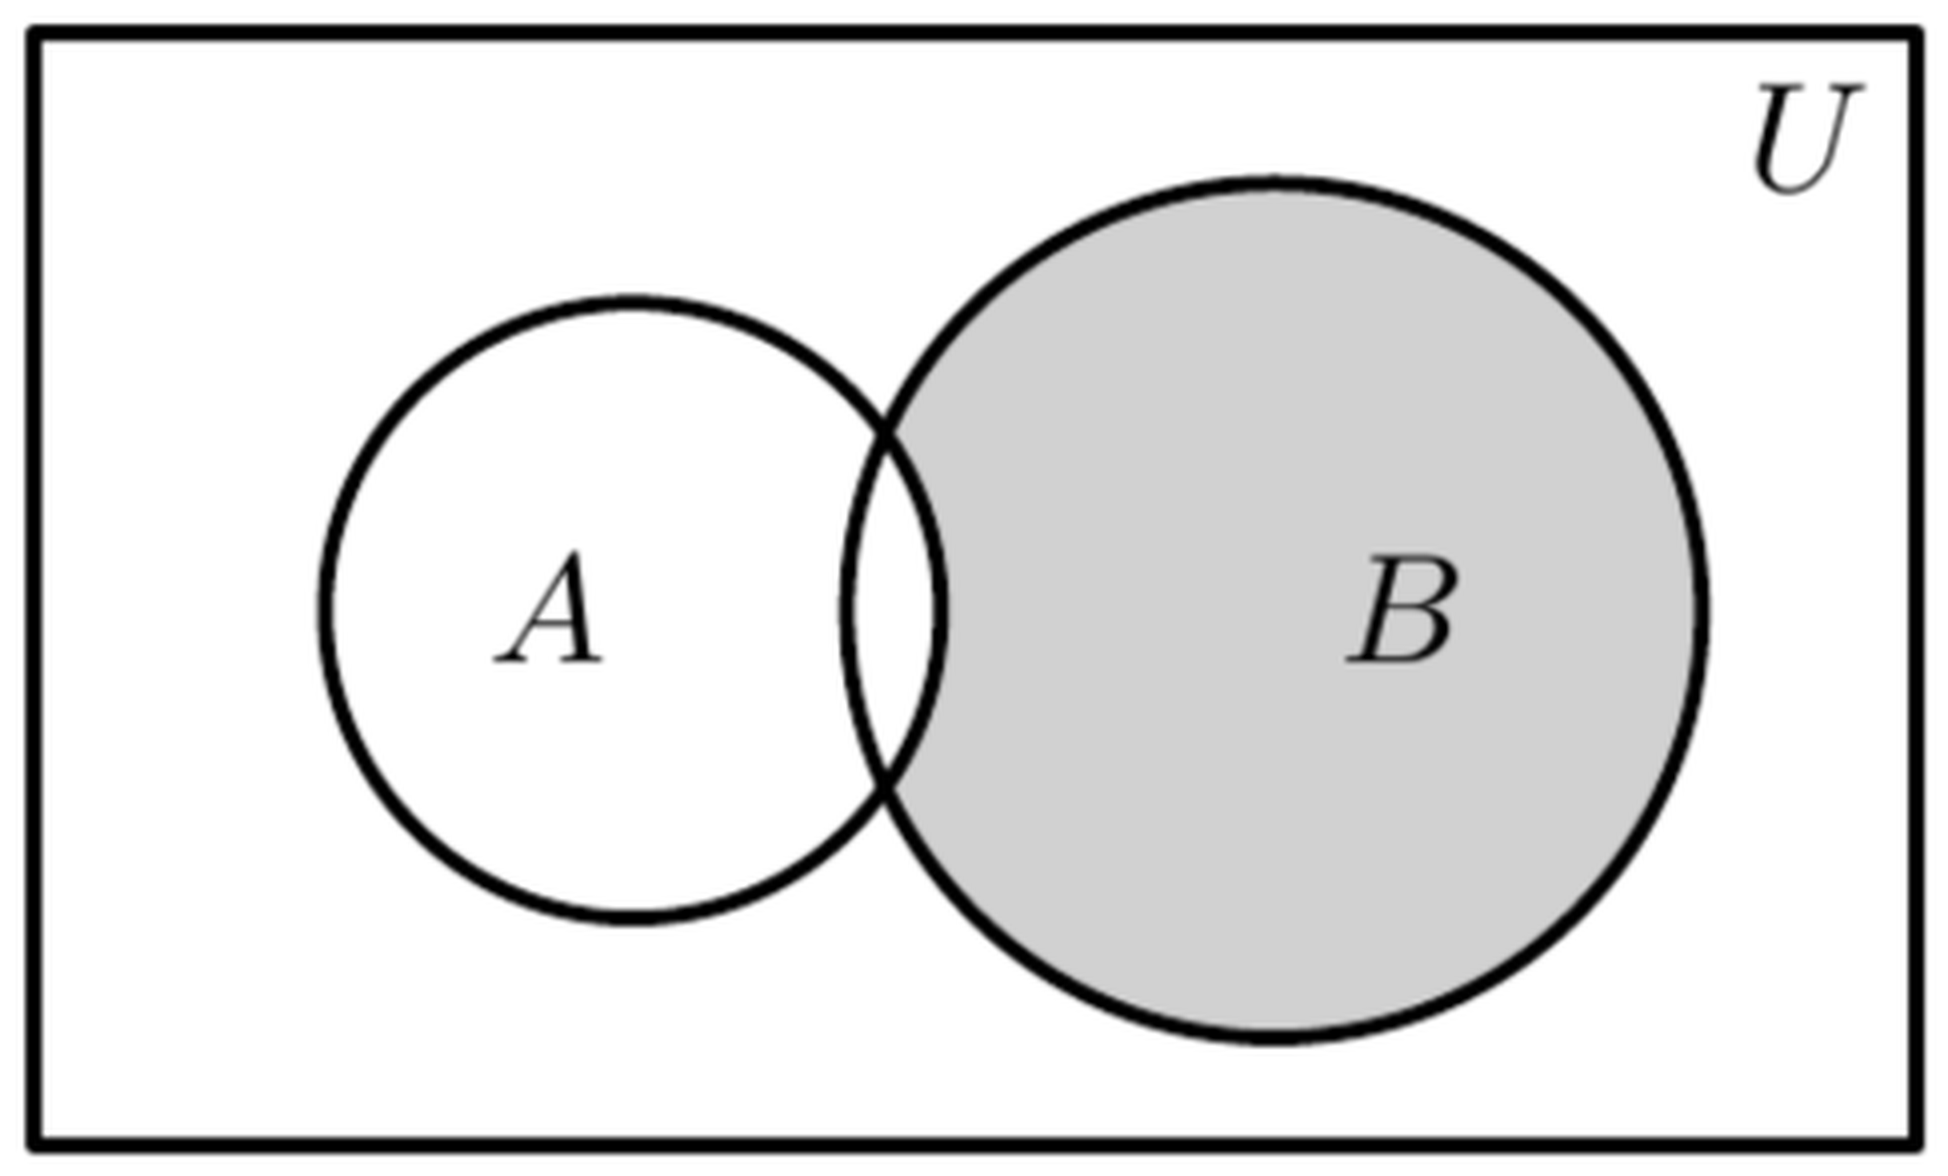
\includegraphics[width=0.38\textwidth]{figures/gao160_q4.png}
\end{center}

\ifanswer
\solbegin
\step{阴影部分表示 $B\cap\overline{A}=\{1,2\}$.}
\solend
\fi

% === Q5 === "图像"（有亻）照录；解析 1 行
\item 已知常数 $a>0$ 且 $a\ne1$，假设无论 $a$ 取何值，函数 $y=\log_a(5x-9)-4$ 的图像恒过一个定点，则这个定点的坐标为\blankline[4.4em].

\ifanswer
\solbegin
\step{$5x-9=1\Rightarrow x=2$，此时 $y=\log_a 1-4=-4$，定点为 $(2,-4)$.}
\solend
\fi

% === Q6 === 解析 2 行
\item 不等式 $(1-2x)^{\frac{3}{4}}>x^{\frac{3}{4}}$ 的解集为\blankline[4.4em].

\ifanswer
\solbegin
\step{定义域为 $\left[0,\dfrac{1}{2}\right]$，由幂函数的单调性，原不等式等价于 $1-2x>x$，}
\step{得 $0\leqslant x<\dfrac{1}{3}$，故解集为 $\left[0,\dfrac{1}{3}\right)$.}
\solend
\fi

% === Q7 === 绝对值 \lvert…\rvert；解析 2 行（跨 01—02 页）
\item 已知不等式 $\lvert x+3\rvert+\lvert x-2\rvert\geqslant 5$，当其等号成立时，$x$ 的取值范围是\blankline[4.4em].

\ifanswer
\solbegin
\step{$\lvert x+3\rvert+\lvert x-2\rvert=\lvert x+3\rvert+\lvert 2-x\rvert\geqslant\lvert(x+3)+(2-x)\rvert=5$，}
\step{等号成立当且仅当 $(x+3)(2-x)\geqslant0$，即 $x\in[-3,2]$.}
\solend
\fi

% === Q8 === 解析 4 行
\item 已知函数 $f(x)=\lvert\log_2 x\rvert$，若方程 $f(x)-t=0$ 有两个不同的实数根 $x_1,x_2$，则 $x_1+x_2$ 的取值范围是\blankline[4.4em].

\ifanswer
\solbegin
\step{方程有两个不同实根，必有 $t>0$，两根为 $2^t,2^{-t}$，}
\step{所以 $x_1+x_2=2^t+2^{-t}>2$（等号仅在 $t=0$ 时成立）.}
\step{任取 $s>2$，令 $a=\dfrac{s+\sqrt{s^2-4}}{2}>1$，取 $t=\log_2 a>0$，则 $x_1+x_2=a+\dfrac{1}{a}=s$，}
\step{所以取值范围为 $(2,+\infty)$.}
\solend
\fi

% === Q9 === 中文弯引号、\R、绝对值 \lvert…\rvert；解析 4 行
\item 已知 $a\in\R$，$b\in\R$，$p:\dfrac{1}{\lvert a\rvert}>\dfrac{1}{\lvert b\rvert}$，$q:\dfrac{1}{a}>\dfrac{1}{b}$，则 $p$ 是 $q$\blankline[4.4em]条件（用“充分非必要”、“必要非充分”、“充要”或“既非充分又非必要”填空）.

\ifanswer
\solbegin
\step{由 $p$、$q$ 中的分式有意义，$a\ne0$ 且 $b\ne0$.}
\step{当 $a=-1,b=-2$ 时，$p$ 成立而 $q$ 不成立，故 $p$ 不是 $q$ 的充分条件.}
\step{当 $a=1,b=-1$ 时，$q$ 成立而 $p$ 不成立，故 $p$ 不是 $q$ 的必要条件.}
\step{故 $p$ 是 $q$ 的充分非必要条件.}
\solend
\fi

% === Q10 === 解析 3 行；其后独立【注】按语 5 行（见头注 ② ⑯、⑤ 1）
\item 已知常数 $a>0$，函数 $y=\dfrac{2^x}{2^x+ax}$ 的图像经过点 $P\left(p,\dfrac{5}{6}\right)$、$Q\left(q,\dfrac{1}{6}\right)$，若 $2^{p+q}=3pq$，则 $a=$\blankline[4.4em].

\ifanswer
\solbegin
\step{由 $\dfrac{2^p}{2^p+ap}=\dfrac{5}{6}$ 得 $2^p=5ap$；由 $\dfrac{2^q}{2^q+aq}=\dfrac{1}{6}$ 得 $2^q=\dfrac{aq}{5}$.}
\step{$2^p>0$，$2^q>0$，$a>0$，得 $p>0$，$q>0$.}
\step{两式相乘得 $2^{p+q}=a^2pq$，又 $2^{p+q}=3pq$ 且 $pq\ne0$，故 $a^2=3$，$a=\sqrt{3}$.}
\solend
% 【注】按语（讲评版编者按，5 个印刷行，仅答案版出，不属于任何题的【解析】）
\stepm{【注】}{按原卷数据严格推敲，点 $Q$ 其实不存在：$a=\sqrt{3}$ 时 $2^q=\dfrac{\sqrt{3}}{5}q<q$；而当 $q>0$}
\step{时，取非负整数 $n$ 使 $n\leqslant q<n+1$，由 $2^{k+1}=2^k+2^k\geqslant2^k+1$ 逐次推得 $2^n\geqslant n+1$，于是}
\step{$2^q\geqslant2^n\geqslant n+1>q$，矛盾. 所以题设条件互相矛盾，严格说本题无解；$\sqrt{3}$ 是由题给关}
\step{系直接推出的值，按命题意图作为答案. 原卷数据疑似有误（同型常见题为 $P\left(p,\dfrac{6}{5}\right)$、}
\step{$Q\left(q,-\dfrac{1}{5}\right)$、$2^{p+q}=36pq$，得 $a=6$）.}% 见头注 ⑤ 1，照录未改
\fi

% === Q11 === 纳皮尔对数材料题；\Z、大数；解析 6 行
\item 17 世纪初，约翰·纳皮尔为了简化计算而发明了对数. 对数的发明是数学史上的重大事件，恩格斯曾经把笛卡尔的坐标系、纳皮尔的对数、牛顿和莱布尼兹的微积分共同称为 17 世纪的三大数学发明. 我们知道，任何一个正实数 $N$ 可以表示成 $N=a\times10^n$ ($1\leqslant a<10,n\in\Z$) 的形式，这便是科学记数法，若两边取常用对数，有 $\lg N=n+\lg a$，则可以估计 $3^{2026}$ 的最高位上的数值为\blankline[4.4em].

\ifanswer
\solbegin
\step{设 $3^{2026}=a\times10^n$ ($1\leqslant a<10,n\in\Z$)，则 $2026\lg 3=n+\lg a$.}
\step{用 $\lg 3\approx 0.4771$ 粗估，得 $2026\lg 3\approx 966.60$.}
\step{为核验误差，用 $0.47712<\lg 3<0.47713$，}
\step{得 $966.64512<2026\lg 3<966.66538$，因此 $n=966$.}
\step{于是 $\lg 4\approx 0.60206<0.64512<\lg a<0.66538<\lg 5\approx 0.69897$，}
\step{所以 $4<a<5$，最高位为 4，估算误差不影响结论.}
\solend
\fi

% === Q12 === 自定义"性质 P"；文本圈数字①②③；解析 19 行（跨 03—05 页）
\item 对于数集 $X=\{-1,x_1,x_2,x_3,\cdots,x_n\}$，其中 $0<x_1<x_2<x_3<\cdots<x_n$，$n\geqslant2$，定义点集 $Y=\{(s,t)\mid s\in X,t\in X\}$，若对于任意 $(s_1,t_1)\in Y$，存在 $(s_2,t_2)\in Y$，使得 $s_1s_2+t_1t_2=0$，则称集合 $X$ 具有性质 $P$. 则下列命题中为真命题的是\blankline[4.4em].

① $X=\{-1,1,2\}$ 具有性质 $P$；②若集合 $X$ 具有性质 $P$，则 $1\in X$；

③集合 $X$ 具有性质 $P$，若 $x_1=\dfrac{1}{2}$，则 $x_n=2$.

\ifanswer
\solbegin
\step{因为 $X=\{-1,1,2\}$，}
\step{所以 $Y=\{(-1,-1),(1,1),(2,2),(-1,1),(-1,2),(1,-1),(1,2),(2,-1),(2,1)\}$，}
\step{由集合 $X$ 具有性质 $P$ 的定义，对于任意 $(s,t)\in Y$，}
\step{若 $s>0$，$t>0$，则 $s=t$ 或 $(s,t)=(1,2)$ 或 $(s,t)=(2,1)$，}
\step{若 $s=t$，取 $s_2=-1$，$t_2=-1$，则 $ss_2+tt_2=0$；}
\step{若 $(s,t)=(1,2)$，取 $s_2=2$，$t_2=-1$，则 $ss_2+tt_2=0$；}
\step{若 $(s,t)=(2,1)$，取 $s_2=-1$，$t_2=2$，则 $ss_2+tt_2=0$；}
\step{若 $s$、$t$ 有一个为负数，则 $s=-1$ 或 $t=-1$，}
\step{若 $s=-1$，则取 $s_2=t$，$t_2=1$，则 $ss_2+tt_2=0$；}
\step{若 $t=-1$，则取 $s_2=1$，$t_2=s$，则 $ss_2+tt_2=0$；故①正确；}
\step{对于任意 $(s_1,t_1)\in Y$，存在 $(s_2,t_2)\in Y$，使得 $s_1s_2+t_1t_2=0$，}
\step{取 $(x_1,x_1)\in Y$，存在 $(x_p,x_q)$ 使得 $x_1x_p+x_1x_q=0$，所以 $x_p+x_q=0$，}
\step{不妨设 $x_p=1$，$x_q=-1$，所以若集合 $X$ 具有性质 $P$，则 $1\in X$，故②正确；}
\step{③假设 $x_n>1$，令 $s_1=\dfrac{1}{2},t_1=x_n$，则存在 $s$、$t\in X$ 使得 $\dfrac{1}{2}s+tx_n=0$，}
\step{同②得 $s$、$t$ 中必有一个数为 $-1$，}
\step{若 $s=-1$，则 $tx_n=\dfrac{1}{2}$，于是 $t=\dfrac{1}{2x_n}<\dfrac{1}{2}=x_1$，矛盾，}
\step{若 $t=-1$，则 $\dfrac{1}{2}s=x_n\cdot(-1)$，于是 $s=2x_n>x_n$，也矛盾，}% 原卷如此（与结论符号不自洽），照录未改，见头注 ⑤ 2
\step{所以 $x_n\leqslant1$，又由②得 $1\in X$，所以 $x_n\geqslant1$，所以 $x_n=1$，故③错误，}
\step{故真命题是①②.}
\solend
\fi

\end{enumerate}

% 答案版里填空解析把页排满，节标题会落到页末、与第 13 题分家（切页审计 B 类）；
% 守卫放 \bigsec 之前，连节标题一起量页高（高一157 成例）
\needvspace{7cm}
\bigsec{二、选择题}

\begin{enumerate}
\setcounter{enumi}{12}

% === Q13 === "图像"照录；解析 1 行，故选 $B$
\item 下列函数中，图像与函数 $y=3^x$ 图像关于 $y$ 轴对称的是\mbox{（\quad）}

\keepwithprev
A. $y=x^3$\qquad B. $y=\left(\dfrac{1}{3}\right)^x$\qquad C. $y=-3^x$\qquad D. $y=\log_3 x$

\ifanswer
\solbegin
\step{将 $x$ 换为 $-x$，得对称图像对应的函数为 $y=3^{-x}=\left(\dfrac{1}{3}\right)^x$，故选 $B$.}
\solend
\fi

% === Q14 === 中文弯引号；解析 2 行（跨 05 页上下），故选 $B$
\item 命题“存在 $x\in(1,+\infty)$，使得 $f(x)>0$”的否定形式为\mbox{（\quad）}

\keepwithprev
A. 不存在 $x\in(-\infty,1]$，使得 $f(x)>0$\qquad B. 对任意 $x\in(1,+\infty)$，有 $f(x)\leqslant0$

C. 对任意 $x\in(-\infty,1]$，有 $f(x)\leqslant0$\qquad D. 存在 $x\in(1,+\infty)$，使得 $f(x)\leqslant0$

\ifanswer
\solbegin
\step{将“存在”改为“对任意”，$x$ 的范围不变，并将 $f(x)>0$ 否定为 $f(x)\leqslant0$，}
\step{故选 $B$.}
\solend
\fi

% === Q15 === \R；四选项两行；解析 3 行，故选 $D$
\item 设 $a>0$，$s\in\R$. 下列各项中，能推出 $a^s>a$ 的一项是\mbox{（\quad）}

\keepwithprev
A. $a>1$，且 $s>0$\qquad B. $a>1$，且 $s<0$

C. $0<a<1$，且 $s>0$\qquad D. $0<a<1$，且 $s<0$

\ifanswer
\solbegin
\step{当 $a>1$ 时，$a^s>a\Leftrightarrow s>1$，A、B 均不能保证.}
\step{当 $0<a<1$ 时，$a^s>a\Leftrightarrow s<1$，C 不能保证，D 中 $s<0<1$，满足要求；}
\step{故选 $D$.}
\solend
\fi

% === Q16 === 题目配图（三版都出）；几何符号 \triangle ABC；解析 3 行，故选 $C$
\needvspace{8cm}
\item 数学说明的方法多种多样，其中利用图形说明就是一种重要方法. 如图所示，在等腰直角三角形 $\triangle ABC$ 中，点 $O$ 为斜边 $AB$ 的中点，点 $D$ 为斜边 $AB$ 上异于顶点的一个动点，设 $AD=a$，$BD=b$，则可用该图形能说明的不等式为\mbox{（\quad）}

\begin{center}
% Q16 等腰直角三角形 ABC 图（C/A/O/D/B 标注）取 05 页右下，去粉色水印、去色、3× LANCZOS 放大；三版都出
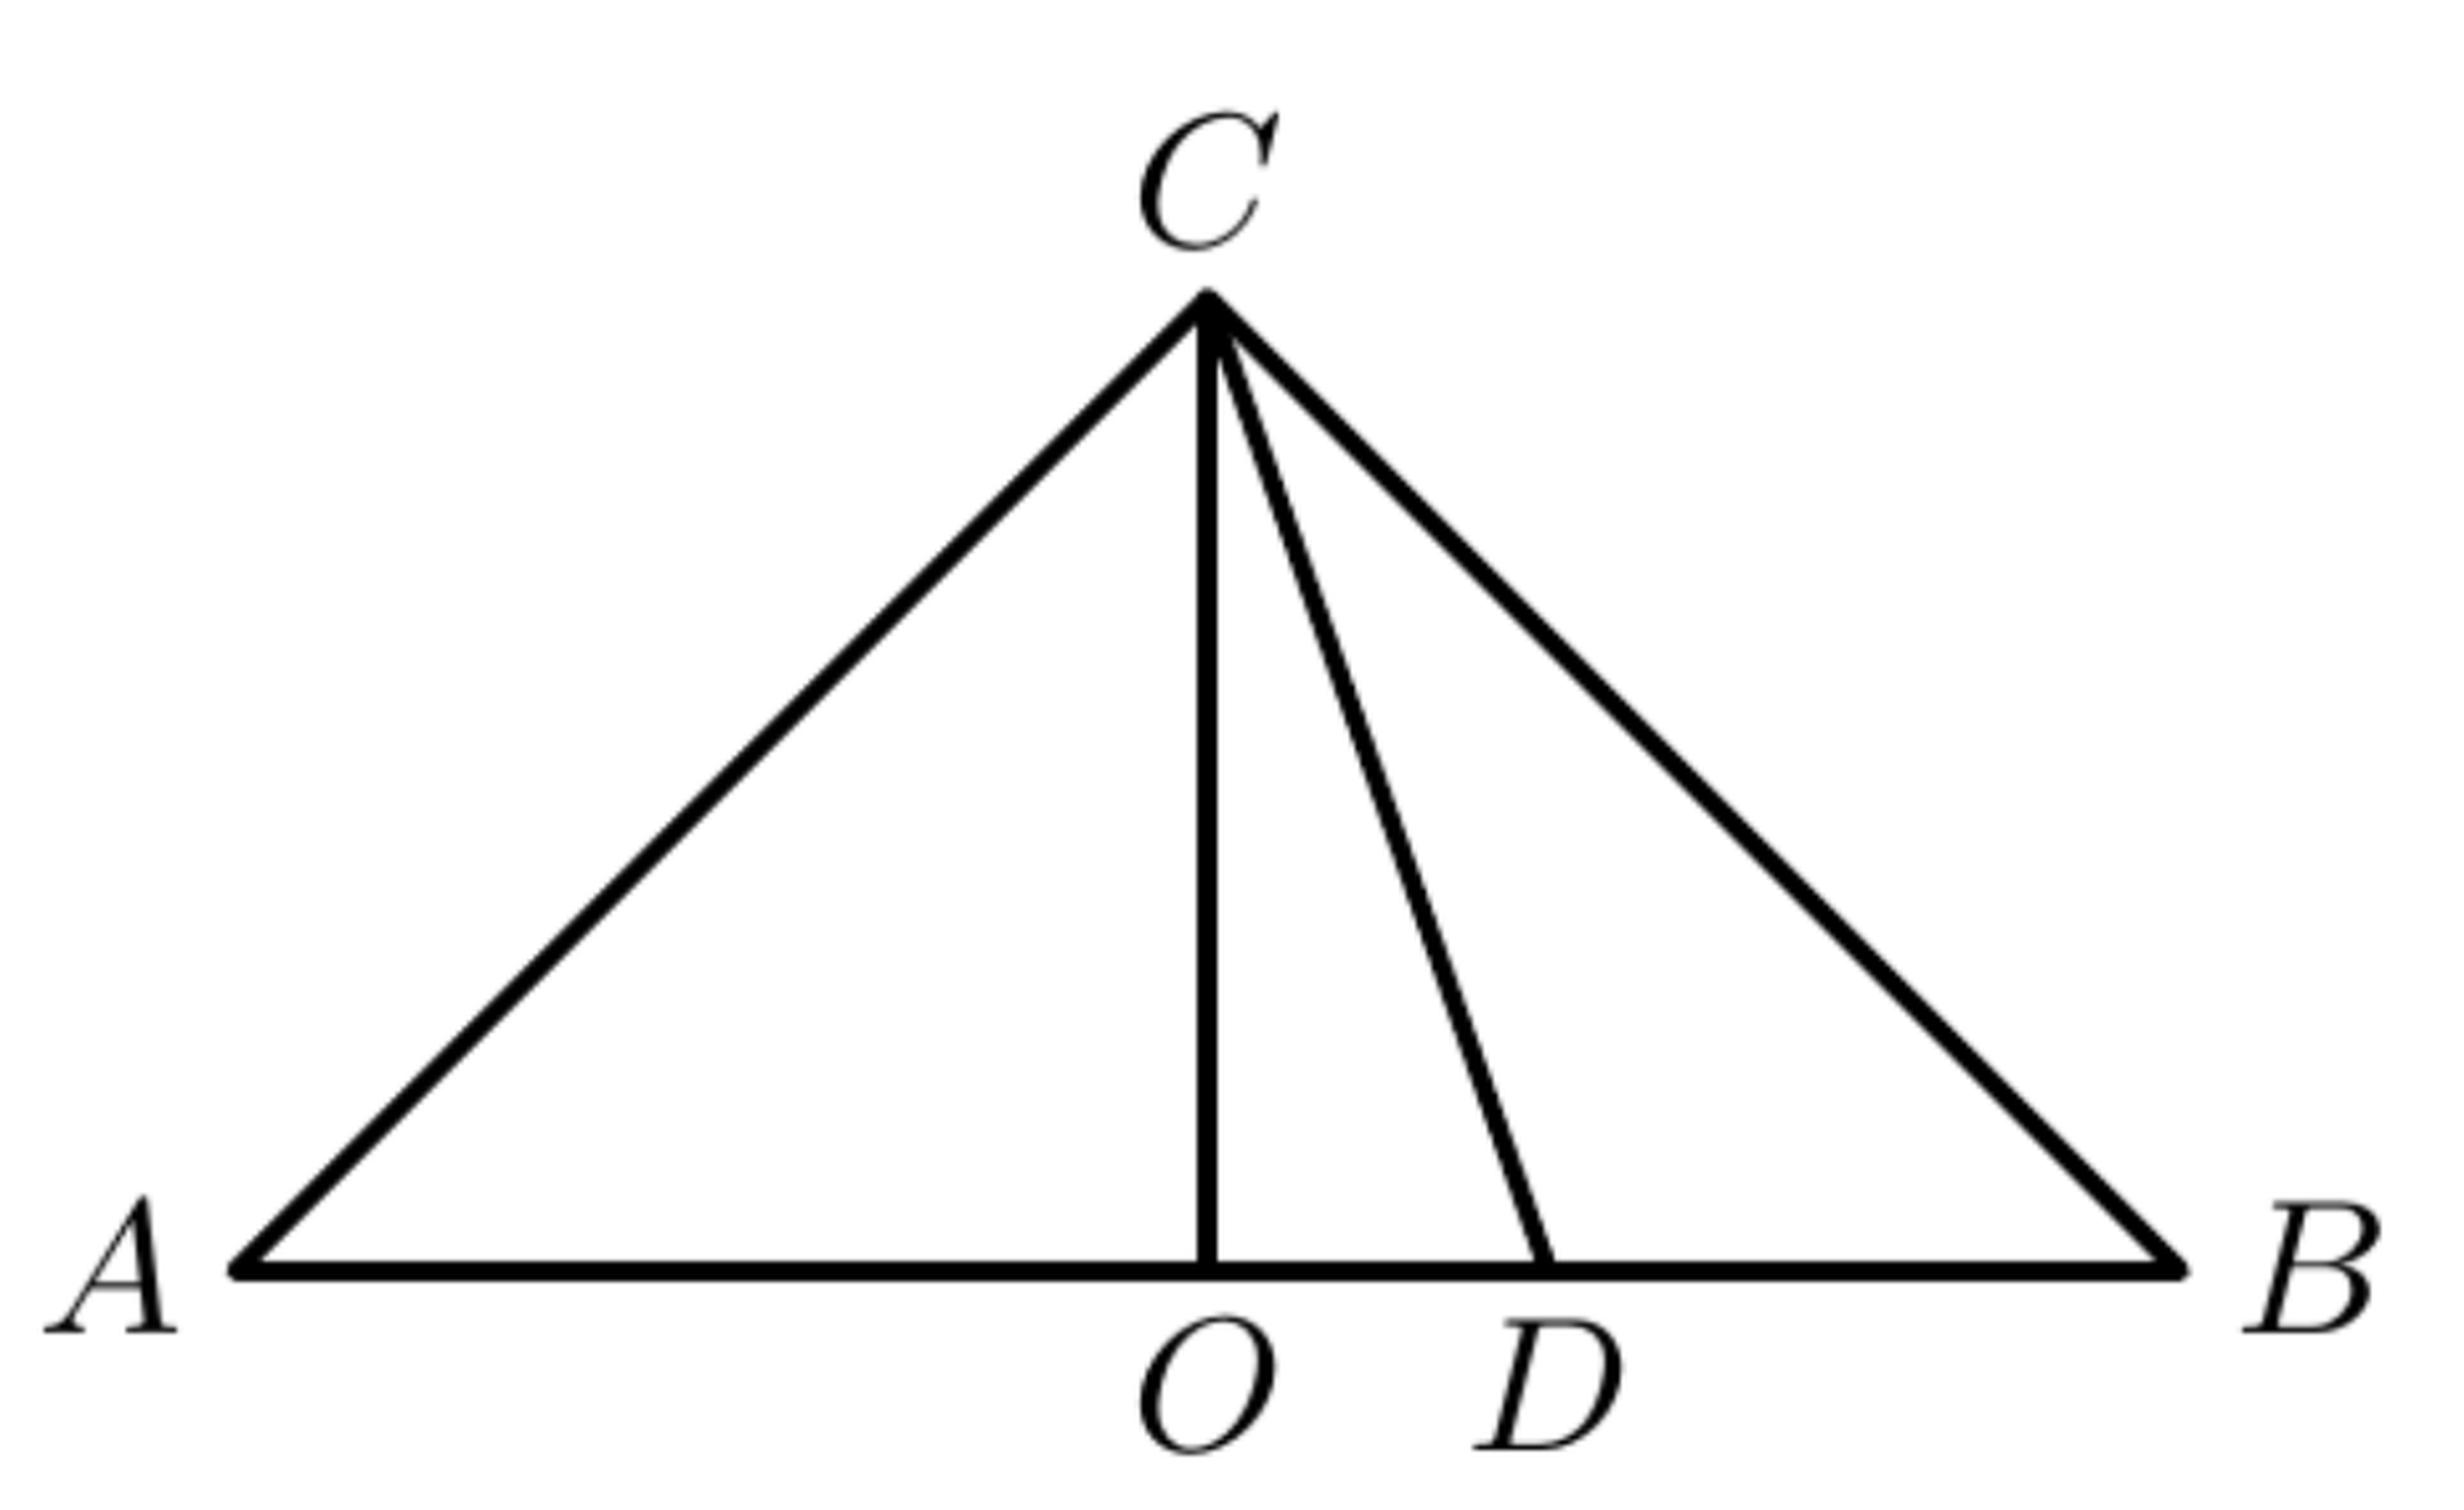
\includegraphics[width=0.34\textwidth]{figures/gao160_q16.png}
\end{center}

\keepwithprev
A. $\dfrac{a+b}{2}\geqslant\sqrt{ab}$ ($a>0,b>0$)\qquad B. $a^2+b^2\geqslant2\sqrt{ab}$ ($a>0,b>0$)

C. $\dfrac{a+b}{2}\leqslant\sqrt{\dfrac{a^2+b^2}{2}}$ ($a>0,b>0$)\qquad D. $\dfrac{2ab}{a+b}\leqslant\sqrt{ab}$ ($a>0,b>0$)

\ifanswer
\solbegin
\step{$CO=AO=\dfrac{a+b}{2},OD=\left\lvert a-\dfrac{a+b}{2}\right\rvert=\dfrac{\lvert a-b\rvert}{2}$，}
\step{$CD=\sqrt{CO^2+OD^2}=\sqrt{\dfrac{a^2+b^2}{2}}\geqslant CO=\dfrac{a+b}{2}$，}
\step{等号当且仅当 $a=b$ 时成立，故选 $C$.}
\solend
\fi

\end{enumerate}

\bigsec{三、解答题}

\begin{enumerate}
\setcounter{enumi}{16}

% === Q17 === cases 块算一行；判别式印等腰偏高三角 \Delta；解析 7 行
\item 已知幂函数 $f(x)=(m^2-2m-2)x^{m-1}$ 在 $(0,+\infty)$ 上是严格增函数.

(1) 求 $m$ 的值；

(2) 若关于 $x$ 的方程 $f(x)=(t+1)x-t^2$ 有两个不相等的正实根，求实数 $t$ 的取值范围.

\ifanswer
\solbegin
\step{(1) 幂函数的系数为 1，因此 $m^2-2m-2=1\Leftrightarrow(m-3)(m+1)=0$，}
\step{解得 $m=3$ 或 $m=-1$.}
\step{由 $f(x)$ 在 $(0,+\infty)$ 上严格递增，得 $m-1>0$，所以 $m=3$，}
\step{此时 $f(x)=x^2$.}
\step{(2) 原方程化为 $x^2-(t+1)x+t^2=0$，}
\step{方程有两个不相等的正实根，则 $\begin{cases}\Delta=(t+1)^2-4t^2=(1-t)(3t+1)>0\\t+1>0\\t^2>0\end{cases}$，}% 判别式原卷印等腰偏高三角 \Delta，照录
\step{得 $t\in\left(-\dfrac{1}{3},0\right)\cup(0,1)$.}
\solend
\fi

% === Q18 === 补集上划线 \overline{A}、\subseteq 带下划线、\varnothing；解析 8 行
\item 已知集合 $A=\{x\mid\lvert x-a\rvert<a-3\}$，$B=\left\{x\mid\dfrac{x+1}{x-2}\geqslant2\right\}$.

(1) 若 $a=5$，求 $\overline{A}\cap B$；

(2) 若 $A\cap B=A$，求实数 $a$ 的取值范围.

\ifanswer
\solbegin
\step{(1) $\dfrac{x+1}{x-2}\geqslant2\Leftrightarrow\dfrac{5-x}{x-2}\geqslant0\Leftrightarrow2<x\leqslant5,B=(2,5]$，}
\step{当 $a=5$ 时，$A=\{x\mid\lvert x-5\rvert<2\}=(3,7)$，于是 $\overline{A}=(-\infty,3]\cup[7,+\infty)$，}
\step{因此 $\overline{A}\cap B=(2,3]$.}
\step{(2) $A\cap B=A$ 等价于 $A\subseteq B$.}
\step{当 $a\leqslant3$ 时，$a-3\leqslant0$，$A=\varnothing$，满足条件.}
\step{当 $a>3$ 时，$\lvert x-a\rvert<a-3\Leftrightarrow3<x<2a-3,A=(3,2a-3)$，}
\step{此时 $A\subseteq B=(2,5]$ 等价于 $2a-3\leqslant5$，即 $a\leqslant4$，结合 $a>3$ 得 $3<a\leqslant4$.}
\step{合并两种情形，实数 $a$ 的取值范围为 $(-\infty,4]$.}
\solend
\fi

% === Q19 === 数据表 tabular 重排（高一130 成例）；cases 块算一行；解析 6 行
\item 作为我国最高水平的综合性运动会，全运会汇聚了国内顶尖体育健儿，某代表队从第 8 届全运会开始登上赛场，且参赛运动员人数逐年递增. 设 $t$ 为该代表队参赛后经过的届数，即第 8 届为 $t=0$，第 9 届为 $t=1$，以此类推. 经过 $t$ 届，运动员人数为 $y$ 人，具体数据如下：

\begin{center}
\begin{tabular}{cccccc}
$t$ & 0 & 1 & 2 & 3 & 4 \\
\hline
届数 & 8 & 9 & 10 & 11 & 12 \\
运动员人数（$y$ 人） & 4 & 11 & 25 & 53 & 109
\end{tabular}
\end{center}

(1) 现有以下两种函数模型：① $y=a\cdot b^t+c$ ($a>0,b>1$)；② $y=\log_a(t+b)+c$ ($b>0,a>1$). 请根据上表中运动员人数的增长规律，选出你认为符合的函数模型（不用说明理由），并利用表中前 3 组数据求出相应的函数解析式；

(2) 若参赛运动员人数按照 (1) 中求得的模型继续增长，在第几届全运会时，该代表队运动员人数将会首次超过 1000 人？

\ifanswer
\solbegin
\step{(1) 选模型①，将前 3 组数据代入，得 $\begin{cases}a+c=4\\ab+c=11\\ab^2+c=25\end{cases}$，}% 原卷印"选模型①"（圈数字①），OCR 误作"四"，照录①，见头注 ⑤ 3
\step{相邻两式相减，得 $a(b-1)=7$，$ab(b-1)=14$，}
\step{两式相除得 $b=2$，进而 $a=7$，$c=-3$，所求函数解析式为 $y=7\cdot2^t-3$.}
\step{(2) $y=7\cdot2^t-3$ 随 $t$ 的增大而增大，且 $t=7$ 时，$y=893<1000$；}
\step{$t=8$ 时，$y=1789>1000$，}
\step{$t$ 为非负整数，首次超过 1000 人时 $t=8$，对应第 $8+8=16$ 届全运会.}
\solend
\fi

% === Q20 === 解析 12 行（跨 08—09 页）
\item 已知函数 $f(x)=\log_a(a-a^x)$.

(1) 求该函数的定义域；

(2) 若 $a>1$，试判断关于 $x$ 的方程 $f(x)=2$ 是否有实数解，并说明理由；

(3) 若当 $x\in(-\infty,0]$ 时，关于 $x$ 的不等式 $f(x)\geqslant-1$ 恒成立，求实数 $a$ 的取值范围.

\ifanswer
\solbegin
\step{(1) 对数的底数须满足 $a>0$ 且 $a\ne1$，真数须满足 $a-a^x>0$，即 $a^x<a^1$.}% 原卷印 $a^1$，照录未化简，见头注 ⑤ 4
\step{当 $a>1$ 时，$x<1$，定义域为 $(-\infty,1)$.}
\step{当 $0<a<1$ 时，$x>1$，定义域为 $(1,+\infty)$.}
\step{(2) 当 $a>1$ 时，若 $f(x)=2$，则 $a-a^x=a^2\Rightarrow a^x=a(1-a)<0$，}
\step{这与 $a^x>0$ 矛盾，因此方程无实数解.}
\step{(3) 不等式在 $(-\infty,0]$ 上恒成立，须先保证该区间包含于函数的定义域，}
\step{由 (1) 得 $a>1$.}
\step{当 $x\leqslant0$ 时，$0<a^x\leqslant1$，所以 $a-a^x\geqslant a-1>0$.}
\step{由对数函数的单调性，$f(x)=\log_a(a-a^x)\geqslant\log_a(a-1)=f(0)$，}
\step{等号当且仅当 $x=0$ 时成立，}
\step{因此所求条件等价于 $\log_a(a-1)\geqslant-1\Leftrightarrow a-1\geqslant\dfrac{1}{a}\Leftrightarrow a^2-a-1\geqslant0$，}
\step{结合 $a>1$，得 $a\in\left[\dfrac{1+\sqrt{5}}{2},+\infty\right)$.}
\solend
\fi

% === Q21 === "和积平衡集"定义证明题；\N；解析 18 行（跨 09—10 页）
\item 已知有限集 $A=\{a_1,a_2,\cdots,a_n\}$ ($n\geqslant2,n\in\N$)，如果 $A$ 中元素 $a_i$ ($i=1,2,3,\cdots,n$) 满足 $a_1+a_2+a_3+\cdots+a_n=a_1\times a_2\times\cdots\times a_n$，就称 $A$ 为“和积平衡集”.

(1) 分别判断集合 $A=\{1,2,3,4\}$，$B=\{4+2\sqrt{2},4-2\sqrt{2}\}$ 是否为“和积平衡集”；

(2) 已知 $a_1$、$a_2$ 是两个不同的正数，且 $\{a_1,a_2\}$ 是“和积平衡集”，请用反证法证明：$a_1$、$a_2$ 至少有一个大于 2；

(3) 若 $a_i\geqslant1$，且 $a_i\in\N$，求所有符合条件的“和积平衡集”.

\ifanswer
\solbegin
\step{(1) 因为 $1+2+3+4=10\ne24=1\times2\times3\times4$，所以 $A$ 不是“和积平衡集”.}
\step{因为 $(4+2\sqrt{2})+(4-2\sqrt{2})=8=(4+2\sqrt{2})(4-2\sqrt{2})$，}
\step{所以 $B$ 是“和积平衡集”.}
\step{(2) 假设 $a_1$、$a_2$ 都不大于 2，则 $\dfrac{1}{a_1}\geqslant\dfrac{1}{2},\dfrac{1}{a_2}\geqslant\dfrac{1}{2}$，}
\step{由于 $a_1\ne a_2$，上述两个不等式至少有一个严格成立.}
\step{而 $a_1+a_2=a_1a_2$，两边除以 $a_1a_2>0$，得 $1=\dfrac{1}{a_1}+\dfrac{1}{a_2}>\dfrac{1}{2}+\dfrac{1}{2}=1$，矛盾，}
\step{所以 $a_1$、$a_2$ 至少有一个大于 2.}
\step{(3) 不妨设 $a_1<a_2<\cdots<a_n$，由各元素均为正整数，得 $a_i\geqslant i$.}
\step{若 $n\geqslant4$，因其余因子均不小于 1，}
\step{有 $a_1a_2\cdots a_n\geqslant a_2a_{n-1}a_n\geqslant2(n-1)a_n>na_n>a_1+a_2+\cdots+a_n$，}
\step{与和积平衡条件矛盾，因此只需讨论 $n=2,3$.}
\step{当 $n=2$ 时，$a_1+a_2=a_1a_2\Leftrightarrow(a_1-1)(a_2-1)=1$，}
\step{两个因子均为非负整数，只能有 $a_1=a_2=2$，与元素互不相同矛盾.}
\step{当 $n=3$ 时，若 $a_1\geqslant2$，则 $a_2\geqslant3$，从而 $a_1a_2a_3\geqslant6a_3>3a_3>a_1+a_2+a_3$，}
\step{矛盾，因此 $a_1=1$.}
\step{此时 $1+a_2+a_3=a_2a_3\Leftrightarrow(a_2-1)(a_3-1)=2$，}
\step{由 $1\leqslant a_2-1<a_3-1$，得 $a_2-1=1$、$a_3-1=2$，即 $a_2=2$、$a_3=3$.}
\step{检验 $1+2+3=1\times2\times3=6$，所求集合为 $\{1,2,3\}$.}
\solend
\fi

\end{enumerate}

\end{document}
"
%
% ① 原始材料：微信公众号"魔都数学加油站"文章，连载"27学年高一160"，原卷卷面标题
% "2026-2027 年奉贤中学高一上期中"（卷面未印副标题、未印连载号）。
% 正文为 10 张 PNG 页（01/04/10 为 2560×3620，02/03/05/06/07/08/09 为
% 4762×6735，同一篇各页分辨率混排，逐页按各自分辨率裁图核对）。
% 体例：讲评版——填空 3—12（10 题）、选择 13—16（4 题）、解答 17—21（5 题），
% 共 19 题，自第 3 题起编（1、2 未印在本篇）；19 题逐题印【解析】，无只印【答案】
% 的题；四道选择题答案在解析末句"故选 $B$/$B$/$D$/$C$"，题干括号
% \mbox{（\quad）} 留空、不另提 \ans{}。题目、答案、解析均据原图转录；卷面粉红色
% 水印"魔都数学加油站"及公众号页脚未录入。
% 全卷插图清单（逐页通读 10 页确认）：2 幅，均为题目配图、三版都出——
%   · Q4 韦恩图（01 页右侧：矩形全集 U、两圆 A/B、阴影部分 B∩上划线 A、
%     标注 U/A/B），裁 figures/gao160_q4.png；
%   · Q16 等腰直角三角形 ABC 图（05 页右下：C 顶点、A/O/D/B 共线底边、
%     CO 与 CD 两条线段），裁 figures/gao160_q16.png；
%   两图均取原卷截图 3—4× LANCZOS 放大、去粉色水印、转灰度、autocontrast；
%   Q4 图左侧题干残字"示"、Q16 图左侧题干残字均已裁白。
%   Q19 有一张 3 行数据表（t／届数／运动员人数（y 人），t=0..4），按全稿
%   成例（高一130）用 tabular 重排，不做成 png；其余各页无题目配图、
%   无解析内配图、无其它表格、无"如图"处。
%
% 卷首标题：原卷印作"2026-2027 年奉贤中学高一上期中"，年份区间按全稿惯例排 en dash；
% 原卷卷面未印副标题，本稿按同期中卷知识模块口径补出"集合与常用逻辑用语、不等式、函数"。
%
% ② 与原卷的排版差异／照录项清单：
%   ① 原文从第 3 题起，本稿保留原题号；共 19 题三节，解答题 5 题到 21；
%      三节各自一个 enumerate + \setcounter{enumi}{2}/{12}/{16}（不贯穿），
%      用 \examtitlest[3] 起手；
%   ② 混合体例说明：19 题全印【解析】、用 \solbegin…\solend，无只印【答案】
%      或答案印括号内的题；四道选择题答案在解析末句"故选 $B$/$B$/$D$/$C$"
%      （逐个放大复核）、括号 \mbox{（\quad）} 留空、不另提 \ans{}；答案版
%      【答案】/【解析】标记数 = 19 = 全卷题数（0 个 \ans ＋ 19 个 \solbegin）；
%   ③ 原卷卷面未印副标题，本稿按知识模块口径补出；
%   ④ 原卷填空横线按全稿惯例排 \blankline[4.4em]；选择题括号排 \mbox{（\quad）}、
%      四道选择题的选项段前按惯例各加 \keepwithprev；解答题不留作答区、不加
%      \anspace（原卷为讲评版，109—113 起全稿不用 \anspace）；
%   ⑤ 数集归一：Q4"$U=\Z$"、Q9"$a\in\R$，$b\in\R$"、Q11"$n\in\Z$"、
%      Q15"$s\in\R$"、Q21"$n\in\N$""$a_i\in\N$"原卷印正体粗体 Z/R/N，
%      按全稿惯例归一 \Z／\R／\N；集合描述竖线排 \mid（Q3、Q4、Q12、
%      Q18、Q21）；空集 \varnothing（Q18 解析 (2)）；补集照原卷上划线排
%      \overline{A}（Q4 解析、Q18 (1) 题干与解析）；子集符号 Q18 两处
%      "$A\subseteq B$"印带下划线 ⊆、照录 \subseteq；
%   ⑥ 绝对值排 \lvert…\rvert（Q7、Q8 题干与解析、Q9 题干、Q16 解析、
%      Q18 题干与解析），Q16 解析的 \left\lvert…\right\rvert 与 \lvert…\rvert
%      均在同一 $…$ 组内配对平衡；
%   ⑦ 判别式两形混用逐处照录不统一（放大逐处确认）：Q3 解析
%      "$\triangle=1^2-4a\times\frac{1}{4}=0$"原卷印扁等边三角、照录
%      \triangle；Q17 解析 cases 块"$\Delta=(t+1)^2-4t^2=(1-t)(3t+1)>0$"
%      原卷印等腰偏高三角、照录 \Delta；Q16 题干几何符号"$\triangle ABC$"
%      按全稿几何三角形记号惯例归一 \triangle（参照 高一150／132 成例）；
%   ⑧ 不等号按全稿惯例排 \leqslant／\geqslant；中文弯引号照录：Q9 题干
%      "充分非必要""必要非充分""充要""既非充分又非必要"、Q14 题干
%      "存在 $x\in(1,+\infty)$，使得 $f(x)>0$"与解析"存在""对任意"、
%      Q21 题干与解析多处"和积平衡集"；注释里一律 ASCII 引号；
%   ⑨ 文本圈数字逐处照录：Q12 题干①②③、Q12 解析"故①正确""同②得"
%      "故②正确""③假设""故③错误""故真命题是①②"、Q19 题干①②与解析
%      "选模型①"，均为印刷圈数字（非 \textcircled、非数学模式）；
%   ⑩ 半角逗号在数学组之间是全稿惯例、非笔误，逐处照录（Q8"$2^t,2^{-t}$"、
%      Q9"$a=-1,b=-2$""$a=1,b=-1$"、Q11"$1\leqslant a<10,n\in\Z$"、
%      Q12"$s_1=\frac{1}{2},t_1=x_n$"、Q16 选项"$a>0,b>0$"与解析
%      "$CO=AO=\frac{a+b}{2},OD=...$"、Q18"$2<x\leqslant5,B=(2,5]$"
%      "$3<x<2a-3,A=(3,2a-3)$"、Q21"$n=2,3$"等）；行中全角逗号／顿号
%      照录（Q15 选项"$a>1$，且 $s>0$"、Q12 解析"$s$、$t$"、Q21 解析
%      "$a_1$、$a_2$"），顿号一律移出数学模式；
%   ⑪ "图像／图象"逐处照录：本卷 Q5"的图像恒过一个定点"、Q10"的图像经过点"、
%      Q13 题干两处"图像"与解析"对称图像对应的函数"均印"图像"（有亻）；
%      Q16 印"图形"（利用图形说明、该图形能说明），无"图象"用例；
%   ⑫ 复杂式照录别简化：Q3 $ax^2+x+\frac14=0$、Q5 $y=\log_a(5x-9)-4$、
%      Q6 $(1-2x)^{\frac34}>x^{\frac34}$ 与 $\left[0,\frac12\right]$、
%      Q8 $\frac{s+\sqrt{s^2-4}}{2}$、Q10 $y=\frac{2^x}{2^x+ax}$ 与
%      $\frac{2^p}{2^p+ap}=\frac56$、$\frac{2^q}{2^q+aq}=\frac16$、
%      Q11 $N=a\times10^n$ 与 $3^{2026}$、$2026\lg3\approx966.60$、
%      $966.64512<2026\lg3<966.66538$、Q12 $Y=\{(s,t)\mid s\in X,t\in X\}$
%      与 $\frac12 s+tx_n=0$、Q16 $\sqrt{\frac{a^2+b^2}{2}}$、
%      Q17 $x^2-(t+1)x+t^2=0$ 与 $\left(-\frac13,0\right)\cup(0,1)$、
%      Q18 $\frac{5-x}{x-2}\geqslant0$、Q19 $y=a\cdot b^t+c$ 与
%      $y=\log_a(t+b)+c$、$y=7\cdot2^t-3$、Q20 $f(x)=\log_a(a-a^x)$
%      与 $a^2-a-1\geqslant0$、$\left[\frac{1+\sqrt5}{2},+\infty\right)$、
%      Q21 $4+2\sqrt2$ 与 $(a_2-1)(a_3-1)=2$ 等；
%   ⑬ 子题标号 (1)(2)(3) 按全稿惯例排半角括号；行末／行中句点按全稿惯例
%      排 ASCII `.`（不是全角「．」）；cases 块整体算一个印刷行
%      （Q17 解析、Q19 解析 (1)）；
%   ⑭ 配图：Q4／Q16 题目配图（三版都出）放 \item 内题干之后 \begin{center}，
%      各用 \needvspace{8cm} 守卫把整块推走，**守卫放在 \item 之前**
%      （见 高一153 Q11/Q19 成例与切页审计 B 类坑）；
%   ⑮ 一条 \step = 原卷解析的一个印刷行；跨上下半页的重叠行只算一次
%      （Q4 解析、Q9 解析首行、Q11 解析首行、Q12 解析"若 $s=-1$…"一行、
%      Q18 解析"此时 $A\subseteq B=(2,5]$…"一行、Q20 (2) 题干、
%      Q21 解析"由 $1\leqslant a_2-1<a_3-1$…"一行）；原卷折行别合并；
%   ⑯ Q10 之后另有一整块【注】按语（03 页上半，5 个印刷行），是讲评版作者对
%      原卷数据自相矛盾的加注、不属于任何题的【解析】。本稿按 高一53
%      "注：…"成例放 Q10 的 \solend 之后、Q10 的 \fi 收尾之前：
%      **整块只保留 Q10 那一层外层 \ifanswer**（那个 \fi 就是 Q10 的收尾），
%      块内 \stepm{【注】}{首行} ＋ 4 条 \step 各自自带内层 \ifanswer…\fi
%      （\step／\stepm 宏内自带，源码里不手动再包一层 \ifanswer，
%      否则 题目溯源.py 的 strip_answers 非贪婪正则会错切）；
%      \stepm 第一参数直接用「【注】」作标签，与全稿 \ans 的【答案】、
%      \solbegin 的【解析】同性质，未加粗以外不另加任何样式；
%      5 行仅答案版出、不新增 \item、不影响溯源，头注 ③ 单列登记、
%      不计入 19 题逐题 \step 账；\stepm 把【注】排成加粗着色标签
%      （原卷为黑色加粗），此一处着色差异在此登记；
%   ⑰ 原卷用字照录：Q11"约翰·纳皮尔""莱布尼兹"（原卷作"兹"，非通行"茨"）、
%      "17 世纪的三大数学发明"；Q16"数学说明的方法""点 $D$ 为斜边 $AB$ 上
%      异于顶点的一个动点"；Q19"登上赛场""以此类推"；
%
% ③ 行数复核：一条 \step = 原卷解析的一个印刷行，cases 块作一个印刷行计。
%   逐题数（逐页核对定稿）：Q3：5；Q4：1；Q5：1；Q6：2；Q7：2；Q8：4；
%   Q9：4；Q10：3；Q11：6；Q12：19；Q13：1；Q14：2；Q15：3；Q16：3；
%   Q17：7；Q18：8；Q19：6；Q20：12；Q21：18。
%   合计 107 条 \step（19 题逐题印刷行账），与原卷逐题印刷行相等。
%   **本卷源码 \step 总数 = 19 题逐题合计 107 ＋ Q10 后独立【注】块 5 行
%   = 112 行**（其中 \step 111 条、\stepm 1 条；\stepm 与 4 条 \step 合为
%   【注】块 5 印刷行）。该 5 行不计入「逐题印刷行」账，也不是任何题的
%   【解析】，而是讲评版编者按语；主会话核验脚本按全文统计 \step 时总数会
%   较逐题账多 5，已与主会话对齐、属已知预期而非错误。
%   全卷 19 题均设 \solbegin…\solend，答案版【答案】/【解析】标记数
%   = 19 = 全卷题数。
%
% ④ 页码分布（供回原图复核）：
%   卷首标题＋"一、填空题"＋Q3 题干＋解析 5 行＋Q4 题干＋韦恩图＋解析
%   1 行＋Q5 题干首行在 01 页上半；Q4 解析（重叠）＋Q5 题干续＋解析 1 行＋
%   Q6 题干＋解析 2 行＋Q7 题干＋解析首行在 01 页下半；Q7 解析末行＋
%   Q8 题干＋解析 4 行＋Q9 题干＋解析首行在 02 页上半；Q9 解析（重叠首行）
%   ＋余 3 行＋Q10 题干＋解析 3 行在 02 页下半；【注】按语 5 行＋Q11 题干＋
%   解析首行在 03 页上半；Q11 解析（重叠首行）＋余 5 行＋Q12 题干＋①②
%   在 03 页下半；Q12 ③＋解析前 9 行在 04 页上半；Q12 解析（重叠 2 行）
%   ＋余 8 行在 04 页下半；Q12 解析末 2 行＋"二、选择题"＋Q13 题干＋选项＋
%   解析 1 行＋Q14 题干＋选项＋解析首行在 05 页上半；Q14 解析末行＋
%   Q15 题干＋选项＋解析 3 行＋Q16 题干＋三角形图在 05 页下半；
%   Q16 选项＋解析 3 行＋"三、解答题"＋Q17 题干＋两问在 06 页上半；
%   Q17 解析 7 行在 06 页下半；Q18 题干＋两问＋解析前 7 行＋Q19 题干首行
%   在 07 页上半；Q18 解析末行（重叠）＋Q19 题干＋表格＋两问在 07 页下半；
%   Q19 解析 6 行＋Q20 题干＋(1)(2) 在 08 页上半；Q20 (2)(3) 题干（重叠）
%   ＋解析 8 行在 08 页下半；Q20 解析末 4 行＋Q21 题干＋(1)(2) 在 09 页
%   上半；Q21 (3)＋解析前 7 行在 09 页下半；Q21 解析 (3) 余 10 行在 10 页
%   上半；Q21 末行（重叠）＋"检验 $1+2+3=1\times2\times3=6$，所求集合为
%   $\{1,2,3\}$."在 10 页下半（此后仅水印、无正文）。本稿按题连排，
%   不丢行、不并折行；全卷末题为第 21 题，无附加题节。
%
% ⑤ 存疑照录（放大原图确认，照录未改、正文对应处另有 % 注）：
%   1. Q10【注】按语：讲评版作者据 $a=\sqrt3$ 时 $2^q=\frac{\sqrt3}{5}q<q$
%      与 $2^n\geqslant n+1$ 推出点 $Q$ 不存在、"严格说本题无解"，并注明
%      "原卷数据疑似有误（同型常见题为 $P(p,\frac65)$、$Q(q,-\frac15)$、
%      $2^{p+q}=36pq$，得 $a=6$）"；本稿照录全块、未删未改（见 ② ⑯）。
%   2. Q12 解析 (3) 末段"若 $t=-1$，则 $\frac{1}{2}s=x_n\cdot(-1)$，
%      于是 $s=2x_n>x_n$，也矛盾，"中，等式右端与紧随的结论符号不自洽
%      （按题意应为 $\frac12 s=x_n$ 或 $-\frac12 s=x_n\cdot(-1)$），逐页
%      放大 04 页确认原卷即如此印、无漏看的负号，照录未改，建议主会话
%      回 04 页再放大复核一次；
%   3. Q19 解析 (1) 印"选模型①"（圈数字①，题干只有①②两种模型）；
%      OCR 误作"选模型四"，放大 08 页确认是①、照录①；
%   4. Q20 解析 (1)"即 $a^x<a^1$"末项原卷印 $a^1$（非 $a$），照录未化简；
%   5. Q11 题干"莱布尼兹"原卷作"兹"（非通行"茨"）、"约翰·纳皮尔"用
%      间隔号·，均照录未改；
%   6. Q9 题干"则 $p$ 是 $q$___条件"与解析"故 $p$ 是 $q$ 的充分非必要条件"
%      句式略异，均照录；
%   7. Q19 解析 (1) 用"前 3 组数据"、题干表格列到 $t=4$，照录未补。
%
\documentclass[a4paper,11pt]{article}
\usepackage{common}

\begin{document}

\examtitlest[3]{2026--2027 年奉贤中学高一上期中}{集合与常用逻辑用语、不等式、函数}

\bigsec{一、填空题}

\begin{enumerate}
\setcounter{enumi}{2}

% === Q3 === 解析 5 行；判别式印扁等边三角 \triangle
\item 若集合 $A=\{x\mid ax^2+x+\dfrac{1}{4}=0\}$ 有且仅有两个子集，则实数 $a=$\blankline[4.4em].

\ifanswer
\solbegin
\step{若集合 $A=\{x\mid ax^2+x+\dfrac{1}{4}=0\}$ 有且仅有两个子集，}
\step{所以方程 $ax^2+x+\dfrac{1}{4}=0$ 只有一个实数根，}
\step{当 $a=0$ 时，方程化为 $x+\dfrac{1}{4}=0$，解得 $x=-\dfrac{1}{4}$，符合题意，}
\step{当 $a\ne0$ 时，则 $\triangle=1^2-4a\times\dfrac{1}{4}=0$，解得 $a=1$，}% 判别式原卷印扁等边三角 \triangle，照录
\step{综上所述，实数 $a=0$ 或 1.}
\solend
\fi

% === Q4 === 题目配图（三版都出）；\needvspace 守卫放 \item 之前；补集上划线 \overline{A}；解析 1 行
\needvspace{8cm}
\item 设全集 $U=\Z$，集合 $A=\{x\mid -3<x<1\}$，$B=\{-1,0,1,2\}$，用列举法表示图中阴影部分为\blankline[4.4em].

\begin{center}
% Q4 韦恩图（全集 U、A/B 两圆、阴影 B∩上划线 A）取 01 页右侧，去粉色水印、去色、4× LANCZOS 放大；三版都出
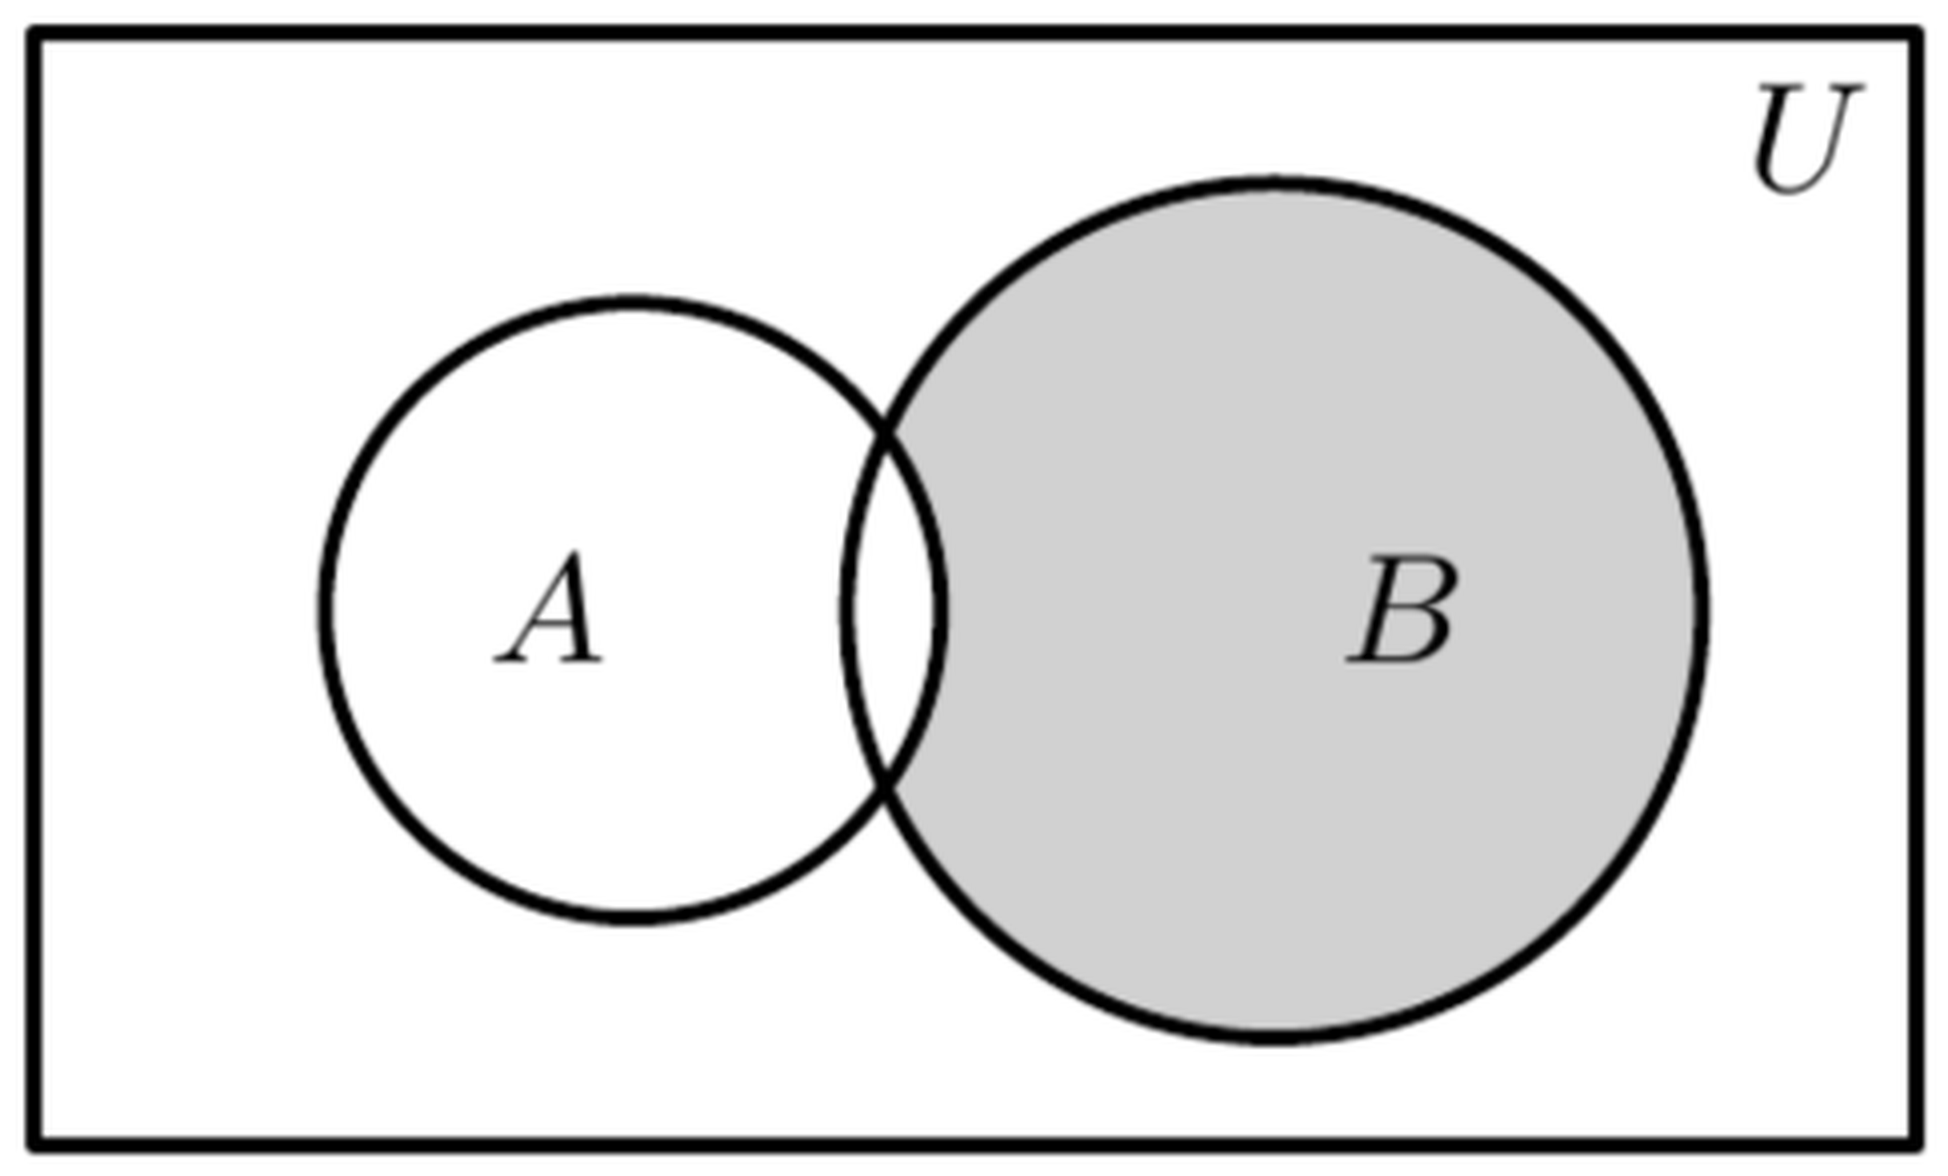
\includegraphics[width=0.38\textwidth]{figures/gao160_q4.png}
\end{center}

\ifanswer
\solbegin
\step{阴影部分表示 $B\cap\overline{A}=\{1,2\}$.}
\solend
\fi

% === Q5 === "图像"（有亻）照录；解析 1 行
\item 已知常数 $a>0$ 且 $a\ne1$，假设无论 $a$ 取何值，函数 $y=\log_a(5x-9)-4$ 的图像恒过一个定点，则这个定点的坐标为\blankline[4.4em].

\ifanswer
\solbegin
\step{$5x-9=1\Rightarrow x=2$，此时 $y=\log_a 1-4=-4$，定点为 $(2,-4)$.}
\solend
\fi

% === Q6 === 解析 2 行
\item 不等式 $(1-2x)^{\frac{3}{4}}>x^{\frac{3}{4}}$ 的解集为\blankline[4.4em].

\ifanswer
\solbegin
\step{定义域为 $\left[0,\dfrac{1}{2}\right]$，由幂函数的单调性，原不等式等价于 $1-2x>x$，}
\step{得 $0\leqslant x<\dfrac{1}{3}$，故解集为 $\left[0,\dfrac{1}{3}\right)$.}
\solend
\fi

% === Q7 === 绝对值 \lvert…\rvert；解析 2 行（跨 01—02 页）
\item 已知不等式 $\lvert x+3\rvert+\lvert x-2\rvert\geqslant 5$，当其等号成立时，$x$ 的取值范围是\blankline[4.4em].

\ifanswer
\solbegin
\step{$\lvert x+3\rvert+\lvert x-2\rvert=\lvert x+3\rvert+\lvert 2-x\rvert\geqslant\lvert(x+3)+(2-x)\rvert=5$，}
\step{等号成立当且仅当 $(x+3)(2-x)\geqslant0$，即 $x\in[-3,2]$.}
\solend
\fi

% === Q8 === 解析 4 行
\item 已知函数 $f(x)=\lvert\log_2 x\rvert$，若方程 $f(x)-t=0$ 有两个不同的实数根 $x_1,x_2$，则 $x_1+x_2$ 的取值范围是\blankline[4.4em].

\ifanswer
\solbegin
\step{方程有两个不同实根，必有 $t>0$，两根为 $2^t,2^{-t}$，}
\step{所以 $x_1+x_2=2^t+2^{-t}>2$（等号仅在 $t=0$ 时成立）.}
\step{任取 $s>2$，令 $a=\dfrac{s+\sqrt{s^2-4}}{2}>1$，取 $t=\log_2 a>0$，则 $x_1+x_2=a+\dfrac{1}{a}=s$，}
\step{所以取值范围为 $(2,+\infty)$.}
\solend
\fi

% === Q9 === 中文弯引号、\R、绝对值 \lvert…\rvert；解析 4 行
\item 已知 $a\in\R$，$b\in\R$，$p:\dfrac{1}{\lvert a\rvert}>\dfrac{1}{\lvert b\rvert}$，$q:\dfrac{1}{a}>\dfrac{1}{b}$，则 $p$ 是 $q$\blankline[4.4em]条件（用“充分非必要”、“必要非充分”、“充要”或“既非充分又非必要”填空）.

\ifanswer
\solbegin
\step{由 $p$、$q$ 中的分式有意义，$a\ne0$ 且 $b\ne0$.}
\step{当 $a=-1,b=-2$ 时，$p$ 成立而 $q$ 不成立，故 $p$ 不是 $q$ 的充分条件.}
\step{当 $a=1,b=-1$ 时，$q$ 成立而 $p$ 不成立，故 $p$ 不是 $q$ 的必要条件.}
\step{故 $p$ 是 $q$ 的充分非必要条件.}
\solend
\fi

% === Q10 === 解析 3 行；其后独立【注】按语 5 行（见头注 ② ⑯、⑤ 1）
\item 已知常数 $a>0$，函数 $y=\dfrac{2^x}{2^x+ax}$ 的图像经过点 $P\left(p,\dfrac{5}{6}\right)$、$Q\left(q,\dfrac{1}{6}\right)$，若 $2^{p+q}=3pq$，则 $a=$\blankline[4.4em].

\ifanswer
\solbegin
\step{由 $\dfrac{2^p}{2^p+ap}=\dfrac{5}{6}$ 得 $2^p=5ap$；由 $\dfrac{2^q}{2^q+aq}=\dfrac{1}{6}$ 得 $2^q=\dfrac{aq}{5}$.}
\step{$2^p>0$，$2^q>0$，$a>0$，得 $p>0$，$q>0$.}
\step{两式相乘得 $2^{p+q}=a^2pq$，又 $2^{p+q}=3pq$ 且 $pq\ne0$，故 $a^2=3$，$a=\sqrt{3}$.}
\solend
% 【注】按语（讲评版编者按，5 个印刷行，仅答案版出，不属于任何题的【解析】）
\stepm{【注】}{按原卷数据严格推敲，点 $Q$ 其实不存在：$a=\sqrt{3}$ 时 $2^q=\dfrac{\sqrt{3}}{5}q<q$；而当 $q>0$}
\step{时，取非负整数 $n$ 使 $n\leqslant q<n+1$，由 $2^{k+1}=2^k+2^k\geqslant2^k+1$ 逐次推得 $2^n\geqslant n+1$，于是}
\step{$2^q\geqslant2^n\geqslant n+1>q$，矛盾. 所以题设条件互相矛盾，严格说本题无解；$\sqrt{3}$ 是由题给关}
\step{系直接推出的值，按命题意图作为答案. 原卷数据疑似有误（同型常见题为 $P\left(p,\dfrac{6}{5}\right)$、}
\step{$Q\left(q,-\dfrac{1}{5}\right)$、$2^{p+q}=36pq$，得 $a=6$）.}% 见头注 ⑤ 1，照录未改
\fi

% === Q11 === 纳皮尔对数材料题；\Z、大数；解析 6 行
\item 17 世纪初，约翰·纳皮尔为了简化计算而发明了对数. 对数的发明是数学史上的重大事件，恩格斯曾经把笛卡尔的坐标系、纳皮尔的对数、牛顿和莱布尼兹的微积分共同称为 17 世纪的三大数学发明. 我们知道，任何一个正实数 $N$ 可以表示成 $N=a\times10^n$ ($1\leqslant a<10,n\in\Z$) 的形式，这便是科学记数法，若两边取常用对数，有 $\lg N=n+\lg a$，则可以估计 $3^{2026}$ 的最高位上的数值为\blankline[4.4em].

\ifanswer
\solbegin
\step{设 $3^{2026}=a\times10^n$ ($1\leqslant a<10,n\in\Z$)，则 $2026\lg 3=n+\lg a$.}
\step{用 $\lg 3\approx 0.4771$ 粗估，得 $2026\lg 3\approx 966.60$.}
\step{为核验误差，用 $0.47712<\lg 3<0.47713$，}
\step{得 $966.64512<2026\lg 3<966.66538$，因此 $n=966$.}
\step{于是 $\lg 4\approx 0.60206<0.64512<\lg a<0.66538<\lg 5\approx 0.69897$，}
\step{所以 $4<a<5$，最高位为 4，估算误差不影响结论.}
\solend
\fi

% === Q12 === 自定义"性质 P"；文本圈数字①②③；解析 19 行（跨 03—05 页）
\item 对于数集 $X=\{-1,x_1,x_2,x_3,\cdots,x_n\}$，其中 $0<x_1<x_2<x_3<\cdots<x_n$，$n\geqslant2$，定义点集 $Y=\{(s,t)\mid s\in X,t\in X\}$，若对于任意 $(s_1,t_1)\in Y$，存在 $(s_2,t_2)\in Y$，使得 $s_1s_2+t_1t_2=0$，则称集合 $X$ 具有性质 $P$. 则下列命题中为真命题的是\blankline[4.4em].

① $X=\{-1,1,2\}$ 具有性质 $P$；②若集合 $X$ 具有性质 $P$，则 $1\in X$；

③集合 $X$ 具有性质 $P$，若 $x_1=\dfrac{1}{2}$，则 $x_n=2$.

\ifanswer
\solbegin
\step{因为 $X=\{-1,1,2\}$，}
\step{所以 $Y=\{(-1,-1),(1,1),(2,2),(-1,1),(-1,2),(1,-1),(1,2),(2,-1),(2,1)\}$，}
\step{由集合 $X$ 具有性质 $P$ 的定义，对于任意 $(s,t)\in Y$，}
\step{若 $s>0$，$t>0$，则 $s=t$ 或 $(s,t)=(1,2)$ 或 $(s,t)=(2,1)$，}
\step{若 $s=t$，取 $s_2=-1$，$t_2=-1$，则 $ss_2+tt_2=0$；}
\step{若 $(s,t)=(1,2)$，取 $s_2=2$，$t_2=-1$，则 $ss_2+tt_2=0$；}
\step{若 $(s,t)=(2,1)$，取 $s_2=-1$，$t_2=2$，则 $ss_2+tt_2=0$；}
\step{若 $s$、$t$ 有一个为负数，则 $s=-1$ 或 $t=-1$，}
\step{若 $s=-1$，则取 $s_2=t$，$t_2=1$，则 $ss_2+tt_2=0$；}
\step{若 $t=-1$，则取 $s_2=1$，$t_2=s$，则 $ss_2+tt_2=0$；故①正确；}
\step{对于任意 $(s_1,t_1)\in Y$，存在 $(s_2,t_2)\in Y$，使得 $s_1s_2+t_1t_2=0$，}
\step{取 $(x_1,x_1)\in Y$，存在 $(x_p,x_q)$ 使得 $x_1x_p+x_1x_q=0$，所以 $x_p+x_q=0$，}
\step{不妨设 $x_p=1$，$x_q=-1$，所以若集合 $X$ 具有性质 $P$，则 $1\in X$，故②正确；}
\step{③假设 $x_n>1$，令 $s_1=\dfrac{1}{2},t_1=x_n$，则存在 $s$、$t\in X$ 使得 $\dfrac{1}{2}s+tx_n=0$，}
\step{同②得 $s$、$t$ 中必有一个数为 $-1$，}
\step{若 $s=-1$，则 $tx_n=\dfrac{1}{2}$，于是 $t=\dfrac{1}{2x_n}<\dfrac{1}{2}=x_1$，矛盾，}
\step{若 $t=-1$，则 $\dfrac{1}{2}s=x_n\cdot(-1)$，于是 $s=2x_n>x_n$，也矛盾，}% 原卷如此（与结论符号不自洽），照录未改，见头注 ⑤ 2
\step{所以 $x_n\leqslant1$，又由②得 $1\in X$，所以 $x_n\geqslant1$，所以 $x_n=1$，故③错误，}
\step{故真命题是①②.}
\solend
\fi

\end{enumerate}

% 答案版里填空解析把页排满，节标题会落到页末、与第 13 题分家（切页审计 B 类）；
% 守卫放 \bigsec 之前，连节标题一起量页高（高一157 成例）
\needvspace{7cm}
\bigsec{二、选择题}

\begin{enumerate}
\setcounter{enumi}{12}

% === Q13 === "图像"照录；解析 1 行，故选 $B$
\item 下列函数中，图像与函数 $y=3^x$ 图像关于 $y$ 轴对称的是\mbox{（\quad）}

\keepwithprev
A. $y=x^3$\qquad B. $y=\left(\dfrac{1}{3}\right)^x$\qquad C. $y=-3^x$\qquad D. $y=\log_3 x$

\ifanswer
\solbegin
\step{将 $x$ 换为 $-x$，得对称图像对应的函数为 $y=3^{-x}=\left(\dfrac{1}{3}\right)^x$，故选 $B$.}
\solend
\fi

% === Q14 === 中文弯引号；解析 2 行（跨 05 页上下），故选 $B$
\item 命题“存在 $x\in(1,+\infty)$，使得 $f(x)>0$”的否定形式为\mbox{（\quad）}

\keepwithprev
A. 不存在 $x\in(-\infty,1]$，使得 $f(x)>0$\qquad B. 对任意 $x\in(1,+\infty)$，有 $f(x)\leqslant0$

C. 对任意 $x\in(-\infty,1]$，有 $f(x)\leqslant0$\qquad D. 存在 $x\in(1,+\infty)$，使得 $f(x)\leqslant0$

\ifanswer
\solbegin
\step{将“存在”改为“对任意”，$x$ 的范围不变，并将 $f(x)>0$ 否定为 $f(x)\leqslant0$，}
\step{故选 $B$.}
\solend
\fi

% === Q15 === \R；四选项两行；解析 3 行，故选 $D$
\item 设 $a>0$，$s\in\R$. 下列各项中，能推出 $a^s>a$ 的一项是\mbox{（\quad）}

\keepwithprev
A. $a>1$，且 $s>0$\qquad B. $a>1$，且 $s<0$

C. $0<a<1$，且 $s>0$\qquad D. $0<a<1$，且 $s<0$

\ifanswer
\solbegin
\step{当 $a>1$ 时，$a^s>a\Leftrightarrow s>1$，A、B 均不能保证.}
\step{当 $0<a<1$ 时，$a^s>a\Leftrightarrow s<1$，C 不能保证，D 中 $s<0<1$，满足要求；}
\step{故选 $D$.}
\solend
\fi

% === Q16 === 题目配图（三版都出）；几何符号 \triangle ABC；解析 3 行，故选 $C$
\needvspace{8cm}
\item 数学说明的方法多种多样，其中利用图形说明就是一种重要方法. 如图所示，在等腰直角三角形 $\triangle ABC$ 中，点 $O$ 为斜边 $AB$ 的中点，点 $D$ 为斜边 $AB$ 上异于顶点的一个动点，设 $AD=a$，$BD=b$，则可用该图形能说明的不等式为\mbox{（\quad）}

\begin{center}
% Q16 等腰直角三角形 ABC 图（C/A/O/D/B 标注）取 05 页右下，去粉色水印、去色、3× LANCZOS 放大；三版都出
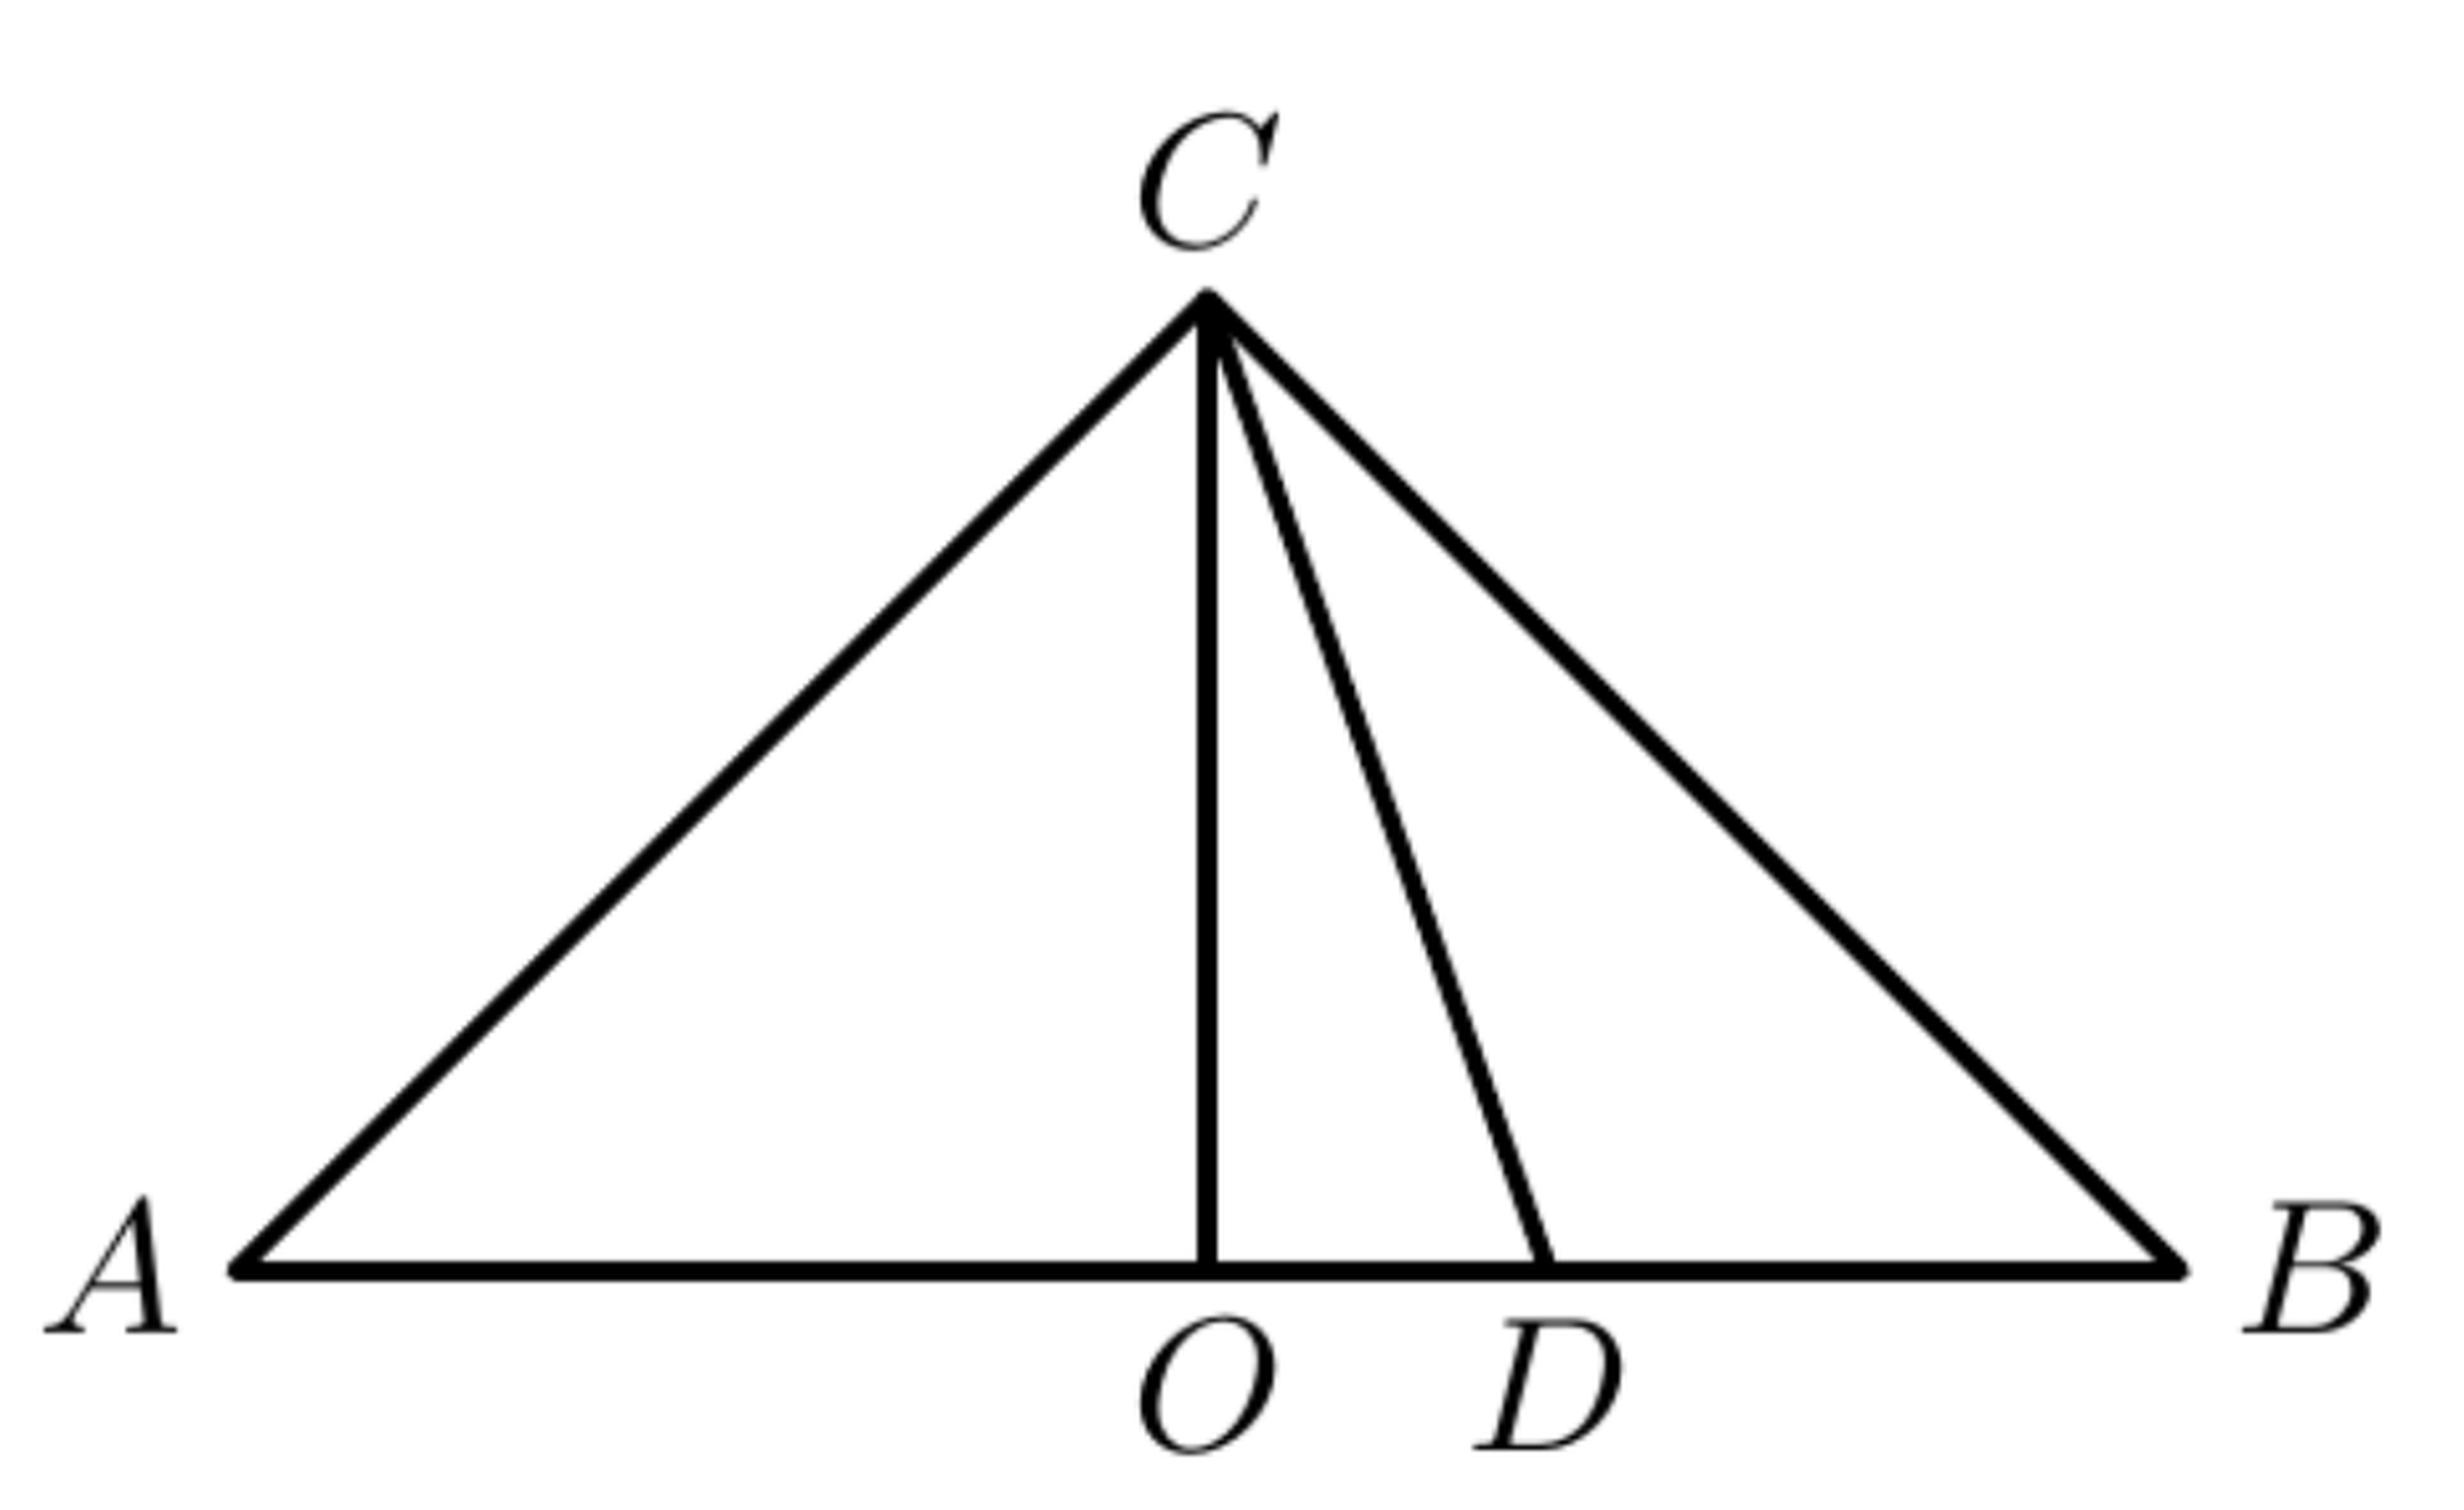
\includegraphics[width=0.34\textwidth]{figures/gao160_q16.png}
\end{center}

\keepwithprev
A. $\dfrac{a+b}{2}\geqslant\sqrt{ab}$ ($a>0,b>0$)\qquad B. $a^2+b^2\geqslant2\sqrt{ab}$ ($a>0,b>0$)

C. $\dfrac{a+b}{2}\leqslant\sqrt{\dfrac{a^2+b^2}{2}}$ ($a>0,b>0$)\qquad D. $\dfrac{2ab}{a+b}\leqslant\sqrt{ab}$ ($a>0,b>0$)

\ifanswer
\solbegin
\step{$CO=AO=\dfrac{a+b}{2},OD=\left\lvert a-\dfrac{a+b}{2}\right\rvert=\dfrac{\lvert a-b\rvert}{2}$，}
\step{$CD=\sqrt{CO^2+OD^2}=\sqrt{\dfrac{a^2+b^2}{2}}\geqslant CO=\dfrac{a+b}{2}$，}
\step{等号当且仅当 $a=b$ 时成立，故选 $C$.}
\solend
\fi

\end{enumerate}

\bigsec{三、解答题}

\begin{enumerate}
\setcounter{enumi}{16}

% === Q17 === cases 块算一行；判别式印等腰偏高三角 \Delta；解析 7 行
\item 已知幂函数 $f(x)=(m^2-2m-2)x^{m-1}$ 在 $(0,+\infty)$ 上是严格增函数.

(1) 求 $m$ 的值；

(2) 若关于 $x$ 的方程 $f(x)=(t+1)x-t^2$ 有两个不相等的正实根，求实数 $t$ 的取值范围.

\ifanswer
\solbegin
\step{(1) 幂函数的系数为 1，因此 $m^2-2m-2=1\Leftrightarrow(m-3)(m+1)=0$，}
\step{解得 $m=3$ 或 $m=-1$.}
\step{由 $f(x)$ 在 $(0,+\infty)$ 上严格递增，得 $m-1>0$，所以 $m=3$，}
\step{此时 $f(x)=x^2$.}
\step{(2) 原方程化为 $x^2-(t+1)x+t^2=0$，}
\step{方程有两个不相等的正实根，则 $\begin{cases}\Delta=(t+1)^2-4t^2=(1-t)(3t+1)>0\\t+1>0\\t^2>0\end{cases}$，}% 判别式原卷印等腰偏高三角 \Delta，照录
\step{得 $t\in\left(-\dfrac{1}{3},0\right)\cup(0,1)$.}
\solend
\fi

% === Q18 === 补集上划线 \overline{A}、\subseteq 带下划线、\varnothing；解析 8 行
\item 已知集合 $A=\{x\mid\lvert x-a\rvert<a-3\}$，$B=\left\{x\mid\dfrac{x+1}{x-2}\geqslant2\right\}$.

(1) 若 $a=5$，求 $\overline{A}\cap B$；

(2) 若 $A\cap B=A$，求实数 $a$ 的取值范围.

\ifanswer
\solbegin
\step{(1) $\dfrac{x+1}{x-2}\geqslant2\Leftrightarrow\dfrac{5-x}{x-2}\geqslant0\Leftrightarrow2<x\leqslant5,B=(2,5]$，}
\step{当 $a=5$ 时，$A=\{x\mid\lvert x-5\rvert<2\}=(3,7)$，于是 $\overline{A}=(-\infty,3]\cup[7,+\infty)$，}
\step{因此 $\overline{A}\cap B=(2,3]$.}
\step{(2) $A\cap B=A$ 等价于 $A\subseteq B$.}
\step{当 $a\leqslant3$ 时，$a-3\leqslant0$，$A=\varnothing$，满足条件.}
\step{当 $a>3$ 时，$\lvert x-a\rvert<a-3\Leftrightarrow3<x<2a-3,A=(3,2a-3)$，}
\step{此时 $A\subseteq B=(2,5]$ 等价于 $2a-3\leqslant5$，即 $a\leqslant4$，结合 $a>3$ 得 $3<a\leqslant4$.}
\step{合并两种情形，实数 $a$ 的取值范围为 $(-\infty,4]$.}
\solend
\fi

% === Q19 === 数据表 tabular 重排（高一130 成例）；cases 块算一行；解析 6 行
\item 作为我国最高水平的综合性运动会，全运会汇聚了国内顶尖体育健儿，某代表队从第 8 届全运会开始登上赛场，且参赛运动员人数逐年递增. 设 $t$ 为该代表队参赛后经过的届数，即第 8 届为 $t=0$，第 9 届为 $t=1$，以此类推. 经过 $t$ 届，运动员人数为 $y$ 人，具体数据如下：

\begin{center}
\begin{tabular}{cccccc}
$t$ & 0 & 1 & 2 & 3 & 4 \\
\hline
届数 & 8 & 9 & 10 & 11 & 12 \\
运动员人数（$y$ 人） & 4 & 11 & 25 & 53 & 109
\end{tabular}
\end{center}

(1) 现有以下两种函数模型：① $y=a\cdot b^t+c$ ($a>0,b>1$)；② $y=\log_a(t+b)+c$ ($b>0,a>1$). 请根据上表中运动员人数的增长规律，选出你认为符合的函数模型（不用说明理由），并利用表中前 3 组数据求出相应的函数解析式；

(2) 若参赛运动员人数按照 (1) 中求得的模型继续增长，在第几届全运会时，该代表队运动员人数将会首次超过 1000 人？

\ifanswer
\solbegin
\step{(1) 选模型①，将前 3 组数据代入，得 $\begin{cases}a+c=4\\ab+c=11\\ab^2+c=25\end{cases}$，}% 原卷印"选模型①"（圈数字①），OCR 误作"四"，照录①，见头注 ⑤ 3
\step{相邻两式相减，得 $a(b-1)=7$，$ab(b-1)=14$，}
\step{两式相除得 $b=2$，进而 $a=7$，$c=-3$，所求函数解析式为 $y=7\cdot2^t-3$.}
\step{(2) $y=7\cdot2^t-3$ 随 $t$ 的增大而增大，且 $t=7$ 时，$y=893<1000$；}
\step{$t=8$ 时，$y=1789>1000$，}
\step{$t$ 为非负整数，首次超过 1000 人时 $t=8$，对应第 $8+8=16$ 届全运会.}
\solend
\fi

% === Q20 === 解析 12 行（跨 08—09 页）
\item 已知函数 $f(x)=\log_a(a-a^x)$.

(1) 求该函数的定义域；

(2) 若 $a>1$，试判断关于 $x$ 的方程 $f(x)=2$ 是否有实数解，并说明理由；

(3) 若当 $x\in(-\infty,0]$ 时，关于 $x$ 的不等式 $f(x)\geqslant-1$ 恒成立，求实数 $a$ 的取值范围.

\ifanswer
\solbegin
\step{(1) 对数的底数须满足 $a>0$ 且 $a\ne1$，真数须满足 $a-a^x>0$，即 $a^x<a^1$.}% 原卷印 $a^1$，照录未化简，见头注 ⑤ 4
\step{当 $a>1$ 时，$x<1$，定义域为 $(-\infty,1)$.}
\step{当 $0<a<1$ 时，$x>1$，定义域为 $(1,+\infty)$.}
\step{(2) 当 $a>1$ 时，若 $f(x)=2$，则 $a-a^x=a^2\Rightarrow a^x=a(1-a)<0$，}
\step{这与 $a^x>0$ 矛盾，因此方程无实数解.}
\step{(3) 不等式在 $(-\infty,0]$ 上恒成立，须先保证该区间包含于函数的定义域，}
\step{由 (1) 得 $a>1$.}
\step{当 $x\leqslant0$ 时，$0<a^x\leqslant1$，所以 $a-a^x\geqslant a-1>0$.}
\step{由对数函数的单调性，$f(x)=\log_a(a-a^x)\geqslant\log_a(a-1)=f(0)$，}
\step{等号当且仅当 $x=0$ 时成立，}
\step{因此所求条件等价于 $\log_a(a-1)\geqslant-1\Leftrightarrow a-1\geqslant\dfrac{1}{a}\Leftrightarrow a^2-a-1\geqslant0$，}
\step{结合 $a>1$，得 $a\in\left[\dfrac{1+\sqrt{5}}{2},+\infty\right)$.}
\solend
\fi

% === Q21 === "和积平衡集"定义证明题；\N；解析 18 行（跨 09—10 页）
\item 已知有限集 $A=\{a_1,a_2,\cdots,a_n\}$ ($n\geqslant2,n\in\N$)，如果 $A$ 中元素 $a_i$ ($i=1,2,3,\cdots,n$) 满足 $a_1+a_2+a_3+\cdots+a_n=a_1\times a_2\times\cdots\times a_n$，就称 $A$ 为“和积平衡集”.

(1) 分别判断集合 $A=\{1,2,3,4\}$，$B=\{4+2\sqrt{2},4-2\sqrt{2}\}$ 是否为“和积平衡集”；

(2) 已知 $a_1$、$a_2$ 是两个不同的正数，且 $\{a_1,a_2\}$ 是“和积平衡集”，请用反证法证明：$a_1$、$a_2$ 至少有一个大于 2；

(3) 若 $a_i\geqslant1$，且 $a_i\in\N$，求所有符合条件的“和积平衡集”.

\ifanswer
\solbegin
\step{(1) 因为 $1+2+3+4=10\ne24=1\times2\times3\times4$，所以 $A$ 不是“和积平衡集”.}
\step{因为 $(4+2\sqrt{2})+(4-2\sqrt{2})=8=(4+2\sqrt{2})(4-2\sqrt{2})$，}
\step{所以 $B$ 是“和积平衡集”.}
\step{(2) 假设 $a_1$、$a_2$ 都不大于 2，则 $\dfrac{1}{a_1}\geqslant\dfrac{1}{2},\dfrac{1}{a_2}\geqslant\dfrac{1}{2}$，}
\step{由于 $a_1\ne a_2$，上述两个不等式至少有一个严格成立.}
\step{而 $a_1+a_2=a_1a_2$，两边除以 $a_1a_2>0$，得 $1=\dfrac{1}{a_1}+\dfrac{1}{a_2}>\dfrac{1}{2}+\dfrac{1}{2}=1$，矛盾，}
\step{所以 $a_1$、$a_2$ 至少有一个大于 2.}
\step{(3) 不妨设 $a_1<a_2<\cdots<a_n$，由各元素均为正整数，得 $a_i\geqslant i$.}
\step{若 $n\geqslant4$，因其余因子均不小于 1，}
\step{有 $a_1a_2\cdots a_n\geqslant a_2a_{n-1}a_n\geqslant2(n-1)a_n>na_n>a_1+a_2+\cdots+a_n$，}
\step{与和积平衡条件矛盾，因此只需讨论 $n=2,3$.}
\step{当 $n=2$ 时，$a_1+a_2=a_1a_2\Leftrightarrow(a_1-1)(a_2-1)=1$，}
\step{两个因子均为非负整数，只能有 $a_1=a_2=2$，与元素互不相同矛盾.}
\step{当 $n=3$ 时，若 $a_1\geqslant2$，则 $a_2\geqslant3$，从而 $a_1a_2a_3\geqslant6a_3>3a_3>a_1+a_2+a_3$，}
\step{矛盾，因此 $a_1=1$.}
\step{此时 $1+a_2+a_3=a_2a_3\Leftrightarrow(a_2-1)(a_3-1)=2$，}
\step{由 $1\leqslant a_2-1<a_3-1$，得 $a_2-1=1$、$a_3-1=2$，即 $a_2=2$、$a_3=3$.}
\step{检验 $1+2+3=1\times2\times3=6$，所求集合为 $\{1,2,3\}$.}
\solend
\fi

\end{enumerate}

\end{document}
"
%
% ① 原始材料：微信公众号"魔都数学加油站"文章，连载"27学年高一160"，原卷卷面标题
% "2026-2027 年奉贤中学高一上期中"（卷面未印副标题、未印连载号）。
% 正文为 10 张 PNG 页（01/04/10 为 2560×3620，02/03/05/06/07/08/09 为
% 4762×6735，同一篇各页分辨率混排，逐页按各自分辨率裁图核对）。
% 体例：讲评版——填空 3—12（10 题）、选择 13—16（4 题）、解答 17—21（5 题），
% 共 19 题，自第 3 题起编（1、2 未印在本篇）；19 题逐题印【解析】，无只印【答案】
% 的题；四道选择题答案在解析末句"故选 $B$/$B$/$D$/$C$"，题干括号
% \mbox{（\quad）} 留空、不另提 \ans{}。题目、答案、解析均据原图转录；卷面粉红色
% 水印"魔都数学加油站"及公众号页脚未录入。
% 全卷插图清单（逐页通读 10 页确认）：2 幅，均为题目配图、三版都出——
%   · Q4 韦恩图（01 页右侧：矩形全集 U、两圆 A/B、阴影部分 B∩上划线 A、
%     标注 U/A/B），裁 figures/gao160_q4.png；
%   · Q16 等腰直角三角形 ABC 图（05 页右下：C 顶点、A/O/D/B 共线底边、
%     CO 与 CD 两条线段），裁 figures/gao160_q16.png；
%   两图均取原卷截图 3—4× LANCZOS 放大、去粉色水印、转灰度、autocontrast；
%   Q4 图左侧题干残字"示"、Q16 图左侧题干残字均已裁白。
%   Q19 有一张 3 行数据表（t／届数／运动员人数（y 人），t=0..4），按全稿
%   成例（高一130）用 tabular 重排，不做成 png；其余各页无题目配图、
%   无解析内配图、无其它表格、无"如图"处。
%
% 卷首标题：原卷印作"2026-2027 年奉贤中学高一上期中"，年份区间按全稿惯例排 en dash；
% 原卷卷面未印副标题，本稿按同期中卷知识模块口径补出"集合与常用逻辑用语、不等式、函数"。
%
% ② 与原卷的排版差异／照录项清单：
%   ① 原文从第 3 题起，本稿保留原题号；共 19 题三节，解答题 5 题到 21；
%      三节各自一个 enumerate + \setcounter{enumi}{2}/{12}/{16}（不贯穿），
%      用 \examtitlest[3] 起手；
%   ② 混合体例说明：19 题全印【解析】、用 \solbegin…\solend，无只印【答案】
%      或答案印括号内的题；四道选择题答案在解析末句"故选 $B$/$B$/$D$/$C$"
%      （逐个放大复核）、括号 \mbox{（\quad）} 留空、不另提 \ans{}；答案版
%      【答案】/【解析】标记数 = 19 = 全卷题数（0 个 \ans ＋ 19 个 \solbegin）；
%   ③ 原卷卷面未印副标题，本稿按知识模块口径补出；
%   ④ 原卷填空横线按全稿惯例排 \blankline[4.4em]；选择题括号排 \mbox{（\quad）}、
%      四道选择题的选项段前按惯例各加 \keepwithprev；解答题不留作答区、不加
%      \anspace（原卷为讲评版，109—113 起全稿不用 \anspace）；
%   ⑤ 数集归一：Q4"$U=\Z$"、Q9"$a\in\R$，$b\in\R$"、Q11"$n\in\Z$"、
%      Q15"$s\in\R$"、Q21"$n\in\N$""$a_i\in\N$"原卷印正体粗体 Z/R/N，
%      按全稿惯例归一 \Z／\R／\N；集合描述竖线排 \mid（Q3、Q4、Q12、
%      Q18、Q21）；空集 \varnothing（Q18 解析 (2)）；补集照原卷上划线排
%      \overline{A}（Q4 解析、Q18 (1) 题干与解析）；子集符号 Q18 两处
%      "$A\subseteq B$"印带下划线 ⊆、照录 \subseteq；
%   ⑥ 绝对值排 \lvert…\rvert（Q7、Q8 题干与解析、Q9 题干、Q16 解析、
%      Q18 题干与解析），Q16 解析的 \left\lvert…\right\rvert 与 \lvert…\rvert
%      均在同一 $…$ 组内配对平衡；
%   ⑦ 判别式两形混用逐处照录不统一（放大逐处确认）：Q3 解析
%      "$\triangle=1^2-4a\times\frac{1}{4}=0$"原卷印扁等边三角、照录
%      \triangle；Q17 解析 cases 块"$\Delta=(t+1)^2-4t^2=(1-t)(3t+1)>0$"
%      原卷印等腰偏高三角、照录 \Delta；Q16 题干几何符号"$\triangle ABC$"
%      按全稿几何三角形记号惯例归一 \triangle（参照 高一150／132 成例）；
%   ⑧ 不等号按全稿惯例排 \leqslant／\geqslant；中文弯引号照录：Q9 题干
%      "充分非必要""必要非充分""充要""既非充分又非必要"、Q14 题干
%      "存在 $x\in(1,+\infty)$，使得 $f(x)>0$"与解析"存在""对任意"、
%      Q21 题干与解析多处"和积平衡集"；注释里一律 ASCII 引号；
%   ⑨ 文本圈数字逐处照录：Q12 题干①②③、Q12 解析"故①正确""同②得"
%      "故②正确""③假设""故③错误""故真命题是①②"、Q19 题干①②与解析
%      "选模型①"，均为印刷圈数字（非 \textcircled、非数学模式）；
%   ⑩ 半角逗号在数学组之间是全稿惯例、非笔误，逐处照录（Q8"$2^t,2^{-t}$"、
%      Q9"$a=-1,b=-2$""$a=1,b=-1$"、Q11"$1\leqslant a<10,n\in\Z$"、
%      Q12"$s_1=\frac{1}{2},t_1=x_n$"、Q16 选项"$a>0,b>0$"与解析
%      "$CO=AO=\frac{a+b}{2},OD=...$"、Q18"$2<x\leqslant5,B=(2,5]$"
%      "$3<x<2a-3,A=(3,2a-3)$"、Q21"$n=2,3$"等）；行中全角逗号／顿号
%      照录（Q15 选项"$a>1$，且 $s>0$"、Q12 解析"$s$、$t$"、Q21 解析
%      "$a_1$、$a_2$"），顿号一律移出数学模式；
%   ⑪ "图像／图象"逐处照录：本卷 Q5"的图像恒过一个定点"、Q10"的图像经过点"、
%      Q13 题干两处"图像"与解析"对称图像对应的函数"均印"图像"（有亻）；
%      Q16 印"图形"（利用图形说明、该图形能说明），无"图象"用例；
%   ⑫ 复杂式照录别简化：Q3 $ax^2+x+\frac14=0$、Q5 $y=\log_a(5x-9)-4$、
%      Q6 $(1-2x)^{\frac34}>x^{\frac34}$ 与 $\left[0,\frac12\right]$、
%      Q8 $\frac{s+\sqrt{s^2-4}}{2}$、Q10 $y=\frac{2^x}{2^x+ax}$ 与
%      $\frac{2^p}{2^p+ap}=\frac56$、$\frac{2^q}{2^q+aq}=\frac16$、
%      Q11 $N=a\times10^n$ 与 $3^{2026}$、$2026\lg3\approx966.60$、
%      $966.64512<2026\lg3<966.66538$、Q12 $Y=\{(s,t)\mid s\in X,t\in X\}$
%      与 $\frac12 s+tx_n=0$、Q16 $\sqrt{\frac{a^2+b^2}{2}}$、
%      Q17 $x^2-(t+1)x+t^2=0$ 与 $\left(-\frac13,0\right)\cup(0,1)$、
%      Q18 $\frac{5-x}{x-2}\geqslant0$、Q19 $y=a\cdot b^t+c$ 与
%      $y=\log_a(t+b)+c$、$y=7\cdot2^t-3$、Q20 $f(x)=\log_a(a-a^x)$
%      与 $a^2-a-1\geqslant0$、$\left[\frac{1+\sqrt5}{2},+\infty\right)$、
%      Q21 $4+2\sqrt2$ 与 $(a_2-1)(a_3-1)=2$ 等；
%   ⑬ 子题标号 (1)(2)(3) 按全稿惯例排半角括号；行末／行中句点按全稿惯例
%      排 ASCII `.`（不是全角「．」）；cases 块整体算一个印刷行
%      （Q17 解析、Q19 解析 (1)）；
%   ⑭ 配图：Q4／Q16 题目配图（三版都出）放 \item 内题干之后 \begin{center}，
%      各用 \needvspace{8cm} 守卫把整块推走，**守卫放在 \item 之前**
%      （见 高一153 Q11/Q19 成例与切页审计 B 类坑）；
%   ⑮ 一条 \step = 原卷解析的一个印刷行；跨上下半页的重叠行只算一次
%      （Q4 解析、Q9 解析首行、Q11 解析首行、Q12 解析"若 $s=-1$…"一行、
%      Q18 解析"此时 $A\subseteq B=(2,5]$…"一行、Q20 (2) 题干、
%      Q21 解析"由 $1\leqslant a_2-1<a_3-1$…"一行）；原卷折行别合并；
%   ⑯ Q10 之后另有一整块【注】按语（03 页上半，5 个印刷行），是讲评版作者对
%      原卷数据自相矛盾的加注、不属于任何题的【解析】。本稿按 高一53
%      "注：…"成例放 Q10 的 \solend 之后、Q10 的 \fi 收尾之前：
%      **整块只保留 Q10 那一层外层 \ifanswer**（那个 \fi 就是 Q10 的收尾），
%      块内 \stepm{【注】}{首行} ＋ 4 条 \step 各自自带内层 \ifanswer…\fi
%      （\step／\stepm 宏内自带，源码里不手动再包一层 \ifanswer，
%      否则 题目溯源.py 的 strip_answers 非贪婪正则会错切）；
%      \stepm 第一参数直接用「【注】」作标签，与全稿 \ans 的【答案】、
%      \solbegin 的【解析】同性质，未加粗以外不另加任何样式；
%      5 行仅答案版出、不新增 \item、不影响溯源，头注 ③ 单列登记、
%      不计入 19 题逐题 \step 账；\stepm 把【注】排成加粗着色标签
%      （原卷为黑色加粗），此一处着色差异在此登记；
%   ⑰ 原卷用字照录：Q11"约翰·纳皮尔""莱布尼兹"（原卷作"兹"，非通行"茨"）、
%      "17 世纪的三大数学发明"；Q16"数学说明的方法""点 $D$ 为斜边 $AB$ 上
%      异于顶点的一个动点"；Q19"登上赛场""以此类推"；
%
% ③ 行数复核：一条 \step = 原卷解析的一个印刷行，cases 块作一个印刷行计。
%   逐题数（逐页核对定稿）：Q3：5；Q4：1；Q5：1；Q6：2；Q7：2；Q8：4；
%   Q9：4；Q10：3；Q11：6；Q12：19；Q13：1；Q14：2；Q15：3；Q16：3；
%   Q17：7；Q18：8；Q19：6；Q20：12；Q21：18。
%   合计 107 条 \step（19 题逐题印刷行账），与原卷逐题印刷行相等。
%   **本卷源码 \step 总数 = 19 题逐题合计 107 ＋ Q10 后独立【注】块 5 行
%   = 112 行**（其中 \step 111 条、\stepm 1 条；\stepm 与 4 条 \step 合为
%   【注】块 5 印刷行）。该 5 行不计入「逐题印刷行」账，也不是任何题的
%   【解析】，而是讲评版编者按语；主会话核验脚本按全文统计 \step 时总数会
%   较逐题账多 5，已与主会话对齐、属已知预期而非错误。
%   全卷 19 题均设 \solbegin…\solend，答案版【答案】/【解析】标记数
%   = 19 = 全卷题数。
%
% ④ 页码分布（供回原图复核）：
%   卷首标题＋"一、填空题"＋Q3 题干＋解析 5 行＋Q4 题干＋韦恩图＋解析
%   1 行＋Q5 题干首行在 01 页上半；Q4 解析（重叠）＋Q5 题干续＋解析 1 行＋
%   Q6 题干＋解析 2 行＋Q7 题干＋解析首行在 01 页下半；Q7 解析末行＋
%   Q8 题干＋解析 4 行＋Q9 题干＋解析首行在 02 页上半；Q9 解析（重叠首行）
%   ＋余 3 行＋Q10 题干＋解析 3 行在 02 页下半；【注】按语 5 行＋Q11 题干＋
%   解析首行在 03 页上半；Q11 解析（重叠首行）＋余 5 行＋Q12 题干＋①②
%   在 03 页下半；Q12 ③＋解析前 9 行在 04 页上半；Q12 解析（重叠 2 行）
%   ＋余 8 行在 04 页下半；Q12 解析末 2 行＋"二、选择题"＋Q13 题干＋选项＋
%   解析 1 行＋Q14 题干＋选项＋解析首行在 05 页上半；Q14 解析末行＋
%   Q15 题干＋选项＋解析 3 行＋Q16 题干＋三角形图在 05 页下半；
%   Q16 选项＋解析 3 行＋"三、解答题"＋Q17 题干＋两问在 06 页上半；
%   Q17 解析 7 行在 06 页下半；Q18 题干＋两问＋解析前 7 行＋Q19 题干首行
%   在 07 页上半；Q18 解析末行（重叠）＋Q19 题干＋表格＋两问在 07 页下半；
%   Q19 解析 6 行＋Q20 题干＋(1)(2) 在 08 页上半；Q20 (2)(3) 题干（重叠）
%   ＋解析 8 行在 08 页下半；Q20 解析末 4 行＋Q21 题干＋(1)(2) 在 09 页
%   上半；Q21 (3)＋解析前 7 行在 09 页下半；Q21 解析 (3) 余 10 行在 10 页
%   上半；Q21 末行（重叠）＋"检验 $1+2+3=1\times2\times3=6$，所求集合为
%   $\{1,2,3\}$."在 10 页下半（此后仅水印、无正文）。本稿按题连排，
%   不丢行、不并折行；全卷末题为第 21 题，无附加题节。
%
% ⑤ 存疑照录（放大原图确认，照录未改、正文对应处另有 % 注）：
%   1. Q10【注】按语：讲评版作者据 $a=\sqrt3$ 时 $2^q=\frac{\sqrt3}{5}q<q$
%      与 $2^n\geqslant n+1$ 推出点 $Q$ 不存在、"严格说本题无解"，并注明
%      "原卷数据疑似有误（同型常见题为 $P(p,\frac65)$、$Q(q,-\frac15)$、
%      $2^{p+q}=36pq$，得 $a=6$）"；本稿照录全块、未删未改（见 ② ⑯）。
%   2. Q12 解析 (3) 末段"若 $t=-1$，则 $\frac{1}{2}s=x_n\cdot(-1)$，
%      于是 $s=2x_n>x_n$，也矛盾，"中，等式右端与紧随的结论符号不自洽
%      （按题意应为 $\frac12 s=x_n$ 或 $-\frac12 s=x_n\cdot(-1)$），逐页
%      放大 04 页确认原卷即如此印、无漏看的负号，照录未改，建议主会话
%      回 04 页再放大复核一次；
%   3. Q19 解析 (1) 印"选模型①"（圈数字①，题干只有①②两种模型）；
%      OCR 误作"选模型四"，放大 08 页确认是①、照录①；
%   4. Q20 解析 (1)"即 $a^x<a^1$"末项原卷印 $a^1$（非 $a$），照录未化简；
%   5. Q11 题干"莱布尼兹"原卷作"兹"（非通行"茨"）、"约翰·纳皮尔"用
%      间隔号·，均照录未改；
%   6. Q9 题干"则 $p$ 是 $q$___条件"与解析"故 $p$ 是 $q$ 的充分非必要条件"
%      句式略异，均照录；
%   7. Q19 解析 (1) 用"前 3 组数据"、题干表格列到 $t=4$，照录未补。
%
\documentclass[a4paper,11pt]{article}
\usepackage{common}

\begin{document}

\examtitlest[3]{2026--2027 年奉贤中学高一上期中}{集合与常用逻辑用语、不等式、函数}

\bigsec{一、填空题}

\begin{enumerate}
\setcounter{enumi}{2}

% === Q3 === 解析 5 行；判别式印扁等边三角 \triangle
\item 若集合 $A=\{x\mid ax^2+x+\dfrac{1}{4}=0\}$ 有且仅有两个子集，则实数 $a=$\blankline[4.4em].

\ifanswer
\solbegin
\step{若集合 $A=\{x\mid ax^2+x+\dfrac{1}{4}=0\}$ 有且仅有两个子集，}
\step{所以方程 $ax^2+x+\dfrac{1}{4}=0$ 只有一个实数根，}
\step{当 $a=0$ 时，方程化为 $x+\dfrac{1}{4}=0$，解得 $x=-\dfrac{1}{4}$，符合题意，}
\step{当 $a\ne0$ 时，则 $\triangle=1^2-4a\times\dfrac{1}{4}=0$，解得 $a=1$，}% 判别式原卷印扁等边三角 \triangle，照录
\step{综上所述，实数 $a=0$ 或 1.}
\solend
\fi

% === Q4 === 题目配图（三版都出）；\needvspace 守卫放 \item 之前；补集上划线 \overline{A}；解析 1 行
\needvspace{8cm}
\item 设全集 $U=\Z$，集合 $A=\{x\mid -3<x<1\}$，$B=\{-1,0,1,2\}$，用列举法表示图中阴影部分为\blankline[4.4em].

\begin{center}
% Q4 韦恩图（全集 U、A/B 两圆、阴影 B∩上划线 A）取 01 页右侧，去粉色水印、去色、4× LANCZOS 放大；三版都出
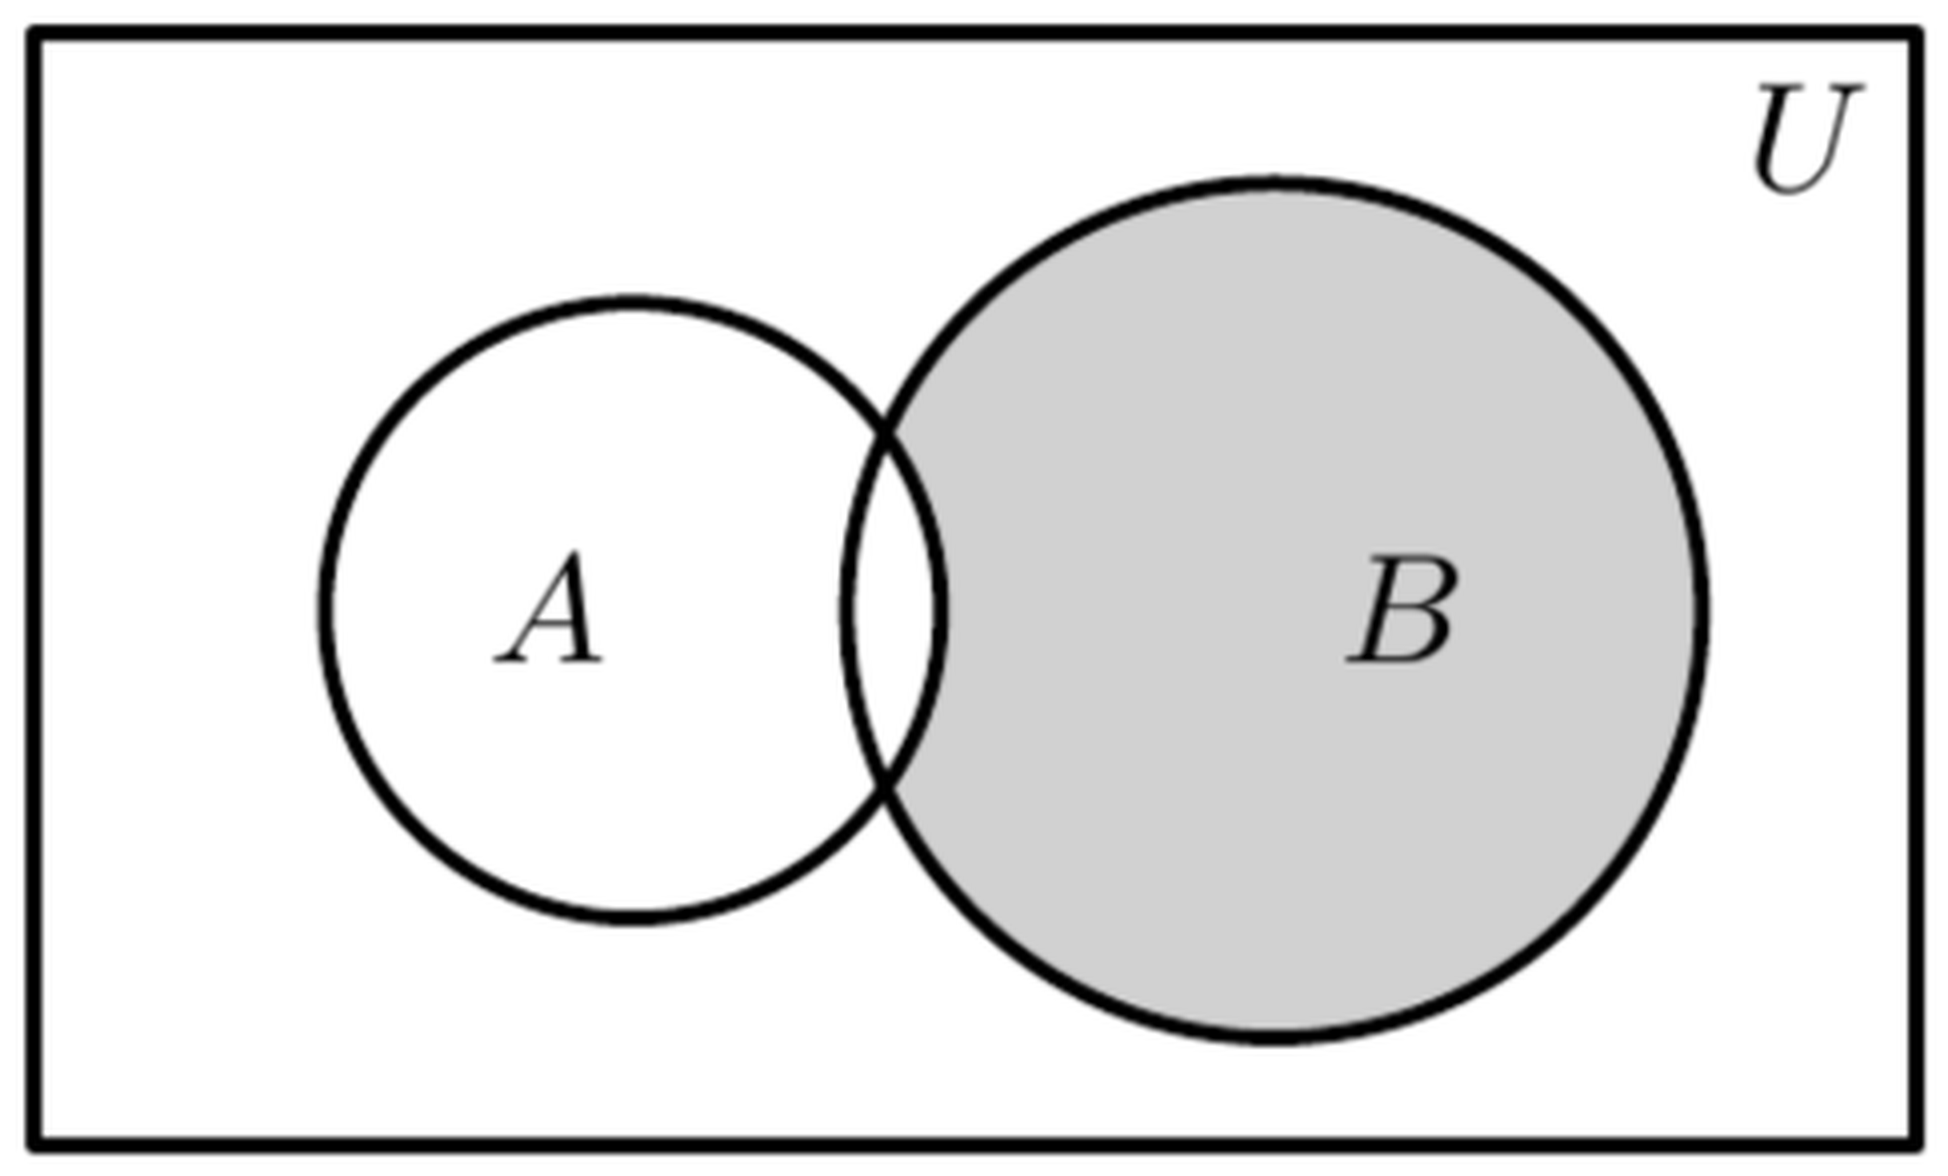
\includegraphics[width=0.38\textwidth]{figures/gao160_q4.png}
\end{center}

\ifanswer
\solbegin
\step{阴影部分表示 $B\cap\overline{A}=\{1,2\}$.}
\solend
\fi

% === Q5 === "图像"（有亻）照录；解析 1 行
\item 已知常数 $a>0$ 且 $a\ne1$，假设无论 $a$ 取何值，函数 $y=\log_a(5x-9)-4$ 的图像恒过一个定点，则这个定点的坐标为\blankline[4.4em].

\ifanswer
\solbegin
\step{$5x-9=1\Rightarrow x=2$，此时 $y=\log_a 1-4=-4$，定点为 $(2,-4)$.}
\solend
\fi

% === Q6 === 解析 2 行
\item 不等式 $(1-2x)^{\frac{3}{4}}>x^{\frac{3}{4}}$ 的解集为\blankline[4.4em].

\ifanswer
\solbegin
\step{定义域为 $\left[0,\dfrac{1}{2}\right]$，由幂函数的单调性，原不等式等价于 $1-2x>x$，}
\step{得 $0\leqslant x<\dfrac{1}{3}$，故解集为 $\left[0,\dfrac{1}{3}\right)$.}
\solend
\fi

% === Q7 === 绝对值 \lvert…\rvert；解析 2 行（跨 01—02 页）
\item 已知不等式 $\lvert x+3\rvert+\lvert x-2\rvert\geqslant 5$，当其等号成立时，$x$ 的取值范围是\blankline[4.4em].

\ifanswer
\solbegin
\step{$\lvert x+3\rvert+\lvert x-2\rvert=\lvert x+3\rvert+\lvert 2-x\rvert\geqslant\lvert(x+3)+(2-x)\rvert=5$，}
\step{等号成立当且仅当 $(x+3)(2-x)\geqslant0$，即 $x\in[-3,2]$.}
\solend
\fi

% === Q8 === 解析 4 行
\item 已知函数 $f(x)=\lvert\log_2 x\rvert$，若方程 $f(x)-t=0$ 有两个不同的实数根 $x_1,x_2$，则 $x_1+x_2$ 的取值范围是\blankline[4.4em].

\ifanswer
\solbegin
\step{方程有两个不同实根，必有 $t>0$，两根为 $2^t,2^{-t}$，}
\step{所以 $x_1+x_2=2^t+2^{-t}>2$（等号仅在 $t=0$ 时成立）.}
\step{任取 $s>2$，令 $a=\dfrac{s+\sqrt{s^2-4}}{2}>1$，取 $t=\log_2 a>0$，则 $x_1+x_2=a+\dfrac{1}{a}=s$，}
\step{所以取值范围为 $(2,+\infty)$.}
\solend
\fi

% === Q9 === 中文弯引号、\R、绝对值 \lvert…\rvert；解析 4 行
\item 已知 $a\in\R$，$b\in\R$，$p:\dfrac{1}{\lvert a\rvert}>\dfrac{1}{\lvert b\rvert}$，$q:\dfrac{1}{a}>\dfrac{1}{b}$，则 $p$ 是 $q$\blankline[4.4em]条件（用“充分非必要”、“必要非充分”、“充要”或“既非充分又非必要”填空）.

\ifanswer
\solbegin
\step{由 $p$、$q$ 中的分式有意义，$a\ne0$ 且 $b\ne0$.}
\step{当 $a=-1,b=-2$ 时，$p$ 成立而 $q$ 不成立，故 $p$ 不是 $q$ 的充分条件.}
\step{当 $a=1,b=-1$ 时，$q$ 成立而 $p$ 不成立，故 $p$ 不是 $q$ 的必要条件.}
\step{故 $p$ 是 $q$ 的充分非必要条件.}
\solend
\fi

% === Q10 === 解析 3 行；其后独立【注】按语 5 行（见头注 ② ⑯、⑤ 1）
\item 已知常数 $a>0$，函数 $y=\dfrac{2^x}{2^x+ax}$ 的图像经过点 $P\left(p,\dfrac{5}{6}\right)$、$Q\left(q,\dfrac{1}{6}\right)$，若 $2^{p+q}=3pq$，则 $a=$\blankline[4.4em].

\ifanswer
\solbegin
\step{由 $\dfrac{2^p}{2^p+ap}=\dfrac{5}{6}$ 得 $2^p=5ap$；由 $\dfrac{2^q}{2^q+aq}=\dfrac{1}{6}$ 得 $2^q=\dfrac{aq}{5}$.}
\step{$2^p>0$，$2^q>0$，$a>0$，得 $p>0$，$q>0$.}
\step{两式相乘得 $2^{p+q}=a^2pq$，又 $2^{p+q}=3pq$ 且 $pq\ne0$，故 $a^2=3$，$a=\sqrt{3}$.}
\solend
% 【注】按语（讲评版编者按，5 个印刷行，仅答案版出，不属于任何题的【解析】）
\stepm{【注】}{按原卷数据严格推敲，点 $Q$ 其实不存在：$a=\sqrt{3}$ 时 $2^q=\dfrac{\sqrt{3}}{5}q<q$；而当 $q>0$}
\step{时，取非负整数 $n$ 使 $n\leqslant q<n+1$，由 $2^{k+1}=2^k+2^k\geqslant2^k+1$ 逐次推得 $2^n\geqslant n+1$，于是}
\step{$2^q\geqslant2^n\geqslant n+1>q$，矛盾. 所以题设条件互相矛盾，严格说本题无解；$\sqrt{3}$ 是由题给关}
\step{系直接推出的值，按命题意图作为答案. 原卷数据疑似有误（同型常见题为 $P\left(p,\dfrac{6}{5}\right)$、}
\step{$Q\left(q,-\dfrac{1}{5}\right)$、$2^{p+q}=36pq$，得 $a=6$）.}% 见头注 ⑤ 1，照录未改
\fi

% === Q11 === 纳皮尔对数材料题；\Z、大数；解析 6 行
\item 17 世纪初，约翰·纳皮尔为了简化计算而发明了对数. 对数的发明是数学史上的重大事件，恩格斯曾经把笛卡尔的坐标系、纳皮尔的对数、牛顿和莱布尼兹的微积分共同称为 17 世纪的三大数学发明. 我们知道，任何一个正实数 $N$ 可以表示成 $N=a\times10^n$ ($1\leqslant a<10,n\in\Z$) 的形式，这便是科学记数法，若两边取常用对数，有 $\lg N=n+\lg a$，则可以估计 $3^{2026}$ 的最高位上的数值为\blankline[4.4em].

\ifanswer
\solbegin
\step{设 $3^{2026}=a\times10^n$ ($1\leqslant a<10,n\in\Z$)，则 $2026\lg 3=n+\lg a$.}
\step{用 $\lg 3\approx 0.4771$ 粗估，得 $2026\lg 3\approx 966.60$.}
\step{为核验误差，用 $0.47712<\lg 3<0.47713$，}
\step{得 $966.64512<2026\lg 3<966.66538$，因此 $n=966$.}
\step{于是 $\lg 4\approx 0.60206<0.64512<\lg a<0.66538<\lg 5\approx 0.69897$，}
\step{所以 $4<a<5$，最高位为 4，估算误差不影响结论.}
\solend
\fi

% === Q12 === 自定义"性质 P"；文本圈数字①②③；解析 19 行（跨 03—05 页）
\item 对于数集 $X=\{-1,x_1,x_2,x_3,\cdots,x_n\}$，其中 $0<x_1<x_2<x_3<\cdots<x_n$，$n\geqslant2$，定义点集 $Y=\{(s,t)\mid s\in X,t\in X\}$，若对于任意 $(s_1,t_1)\in Y$，存在 $(s_2,t_2)\in Y$，使得 $s_1s_2+t_1t_2=0$，则称集合 $X$ 具有性质 $P$. 则下列命题中为真命题的是\blankline[4.4em].

① $X=\{-1,1,2\}$ 具有性质 $P$；②若集合 $X$ 具有性质 $P$，则 $1\in X$；

③集合 $X$ 具有性质 $P$，若 $x_1=\dfrac{1}{2}$，则 $x_n=2$.

\ifanswer
\solbegin
\step{因为 $X=\{-1,1,2\}$，}
\step{所以 $Y=\{(-1,-1),(1,1),(2,2),(-1,1),(-1,2),(1,-1),(1,2),(2,-1),(2,1)\}$，}
\step{由集合 $X$ 具有性质 $P$ 的定义，对于任意 $(s,t)\in Y$，}
\step{若 $s>0$，$t>0$，则 $s=t$ 或 $(s,t)=(1,2)$ 或 $(s,t)=(2,1)$，}
\step{若 $s=t$，取 $s_2=-1$，$t_2=-1$，则 $ss_2+tt_2=0$；}
\step{若 $(s,t)=(1,2)$，取 $s_2=2$，$t_2=-1$，则 $ss_2+tt_2=0$；}
\step{若 $(s,t)=(2,1)$，取 $s_2=-1$，$t_2=2$，则 $ss_2+tt_2=0$；}
\step{若 $s$、$t$ 有一个为负数，则 $s=-1$ 或 $t=-1$，}
\step{若 $s=-1$，则取 $s_2=t$，$t_2=1$，则 $ss_2+tt_2=0$；}
\step{若 $t=-1$，则取 $s_2=1$，$t_2=s$，则 $ss_2+tt_2=0$；故①正确；}
\step{对于任意 $(s_1,t_1)\in Y$，存在 $(s_2,t_2)\in Y$，使得 $s_1s_2+t_1t_2=0$，}
\step{取 $(x_1,x_1)\in Y$，存在 $(x_p,x_q)$ 使得 $x_1x_p+x_1x_q=0$，所以 $x_p+x_q=0$，}
\step{不妨设 $x_p=1$，$x_q=-1$，所以若集合 $X$ 具有性质 $P$，则 $1\in X$，故②正确；}
\step{③假设 $x_n>1$，令 $s_1=\dfrac{1}{2},t_1=x_n$，则存在 $s$、$t\in X$ 使得 $\dfrac{1}{2}s+tx_n=0$，}
\step{同②得 $s$、$t$ 中必有一个数为 $-1$，}
\step{若 $s=-1$，则 $tx_n=\dfrac{1}{2}$，于是 $t=\dfrac{1}{2x_n}<\dfrac{1}{2}=x_1$，矛盾，}
\step{若 $t=-1$，则 $\dfrac{1}{2}s=x_n\cdot(-1)$，于是 $s=2x_n>x_n$，也矛盾，}% 原卷如此（与结论符号不自洽），照录未改，见头注 ⑤ 2
\step{所以 $x_n\leqslant1$，又由②得 $1\in X$，所以 $x_n\geqslant1$，所以 $x_n=1$，故③错误，}
\step{故真命题是①②.}
\solend
\fi

\end{enumerate}

% 答案版里填空解析把页排满，节标题会落到页末、与第 13 题分家（切页审计 B 类）；
% 守卫放 \bigsec 之前，连节标题一起量页高（高一157 成例）
\needvspace{7cm}
\bigsec{二、选择题}

\begin{enumerate}
\setcounter{enumi}{12}

% === Q13 === "图像"照录；解析 1 行，故选 $B$
\item 下列函数中，图像与函数 $y=3^x$ 图像关于 $y$ 轴对称的是\mbox{（\quad）}

\keepwithprev
A. $y=x^3$\qquad B. $y=\left(\dfrac{1}{3}\right)^x$\qquad C. $y=-3^x$\qquad D. $y=\log_3 x$

\ifanswer
\solbegin
\step{将 $x$ 换为 $-x$，得对称图像对应的函数为 $y=3^{-x}=\left(\dfrac{1}{3}\right)^x$，故选 $B$.}
\solend
\fi

% === Q14 === 中文弯引号；解析 2 行（跨 05 页上下），故选 $B$
\item 命题“存在 $x\in(1,+\infty)$，使得 $f(x)>0$”的否定形式为\mbox{（\quad）}

\keepwithprev
A. 不存在 $x\in(-\infty,1]$，使得 $f(x)>0$\qquad B. 对任意 $x\in(1,+\infty)$，有 $f(x)\leqslant0$

C. 对任意 $x\in(-\infty,1]$，有 $f(x)\leqslant0$\qquad D. 存在 $x\in(1,+\infty)$，使得 $f(x)\leqslant0$

\ifanswer
\solbegin
\step{将“存在”改为“对任意”，$x$ 的范围不变，并将 $f(x)>0$ 否定为 $f(x)\leqslant0$，}
\step{故选 $B$.}
\solend
\fi

% === Q15 === \R；四选项两行；解析 3 行，故选 $D$
\item 设 $a>0$，$s\in\R$. 下列各项中，能推出 $a^s>a$ 的一项是\mbox{（\quad）}

\keepwithprev
A. $a>1$，且 $s>0$\qquad B. $a>1$，且 $s<0$

C. $0<a<1$，且 $s>0$\qquad D. $0<a<1$，且 $s<0$

\ifanswer
\solbegin
\step{当 $a>1$ 时，$a^s>a\Leftrightarrow s>1$，A、B 均不能保证.}
\step{当 $0<a<1$ 时，$a^s>a\Leftrightarrow s<1$，C 不能保证，D 中 $s<0<1$，满足要求；}
\step{故选 $D$.}
\solend
\fi

% === Q16 === 题目配图（三版都出）；几何符号 \triangle ABC；解析 3 行，故选 $C$
\needvspace{8cm}
\item 数学说明的方法多种多样，其中利用图形说明就是一种重要方法. 如图所示，在等腰直角三角形 $\triangle ABC$ 中，点 $O$ 为斜边 $AB$ 的中点，点 $D$ 为斜边 $AB$ 上异于顶点的一个动点，设 $AD=a$，$BD=b$，则可用该图形能说明的不等式为\mbox{（\quad）}

\begin{center}
% Q16 等腰直角三角形 ABC 图（C/A/O/D/B 标注）取 05 页右下，去粉色水印、去色、3× LANCZOS 放大；三版都出
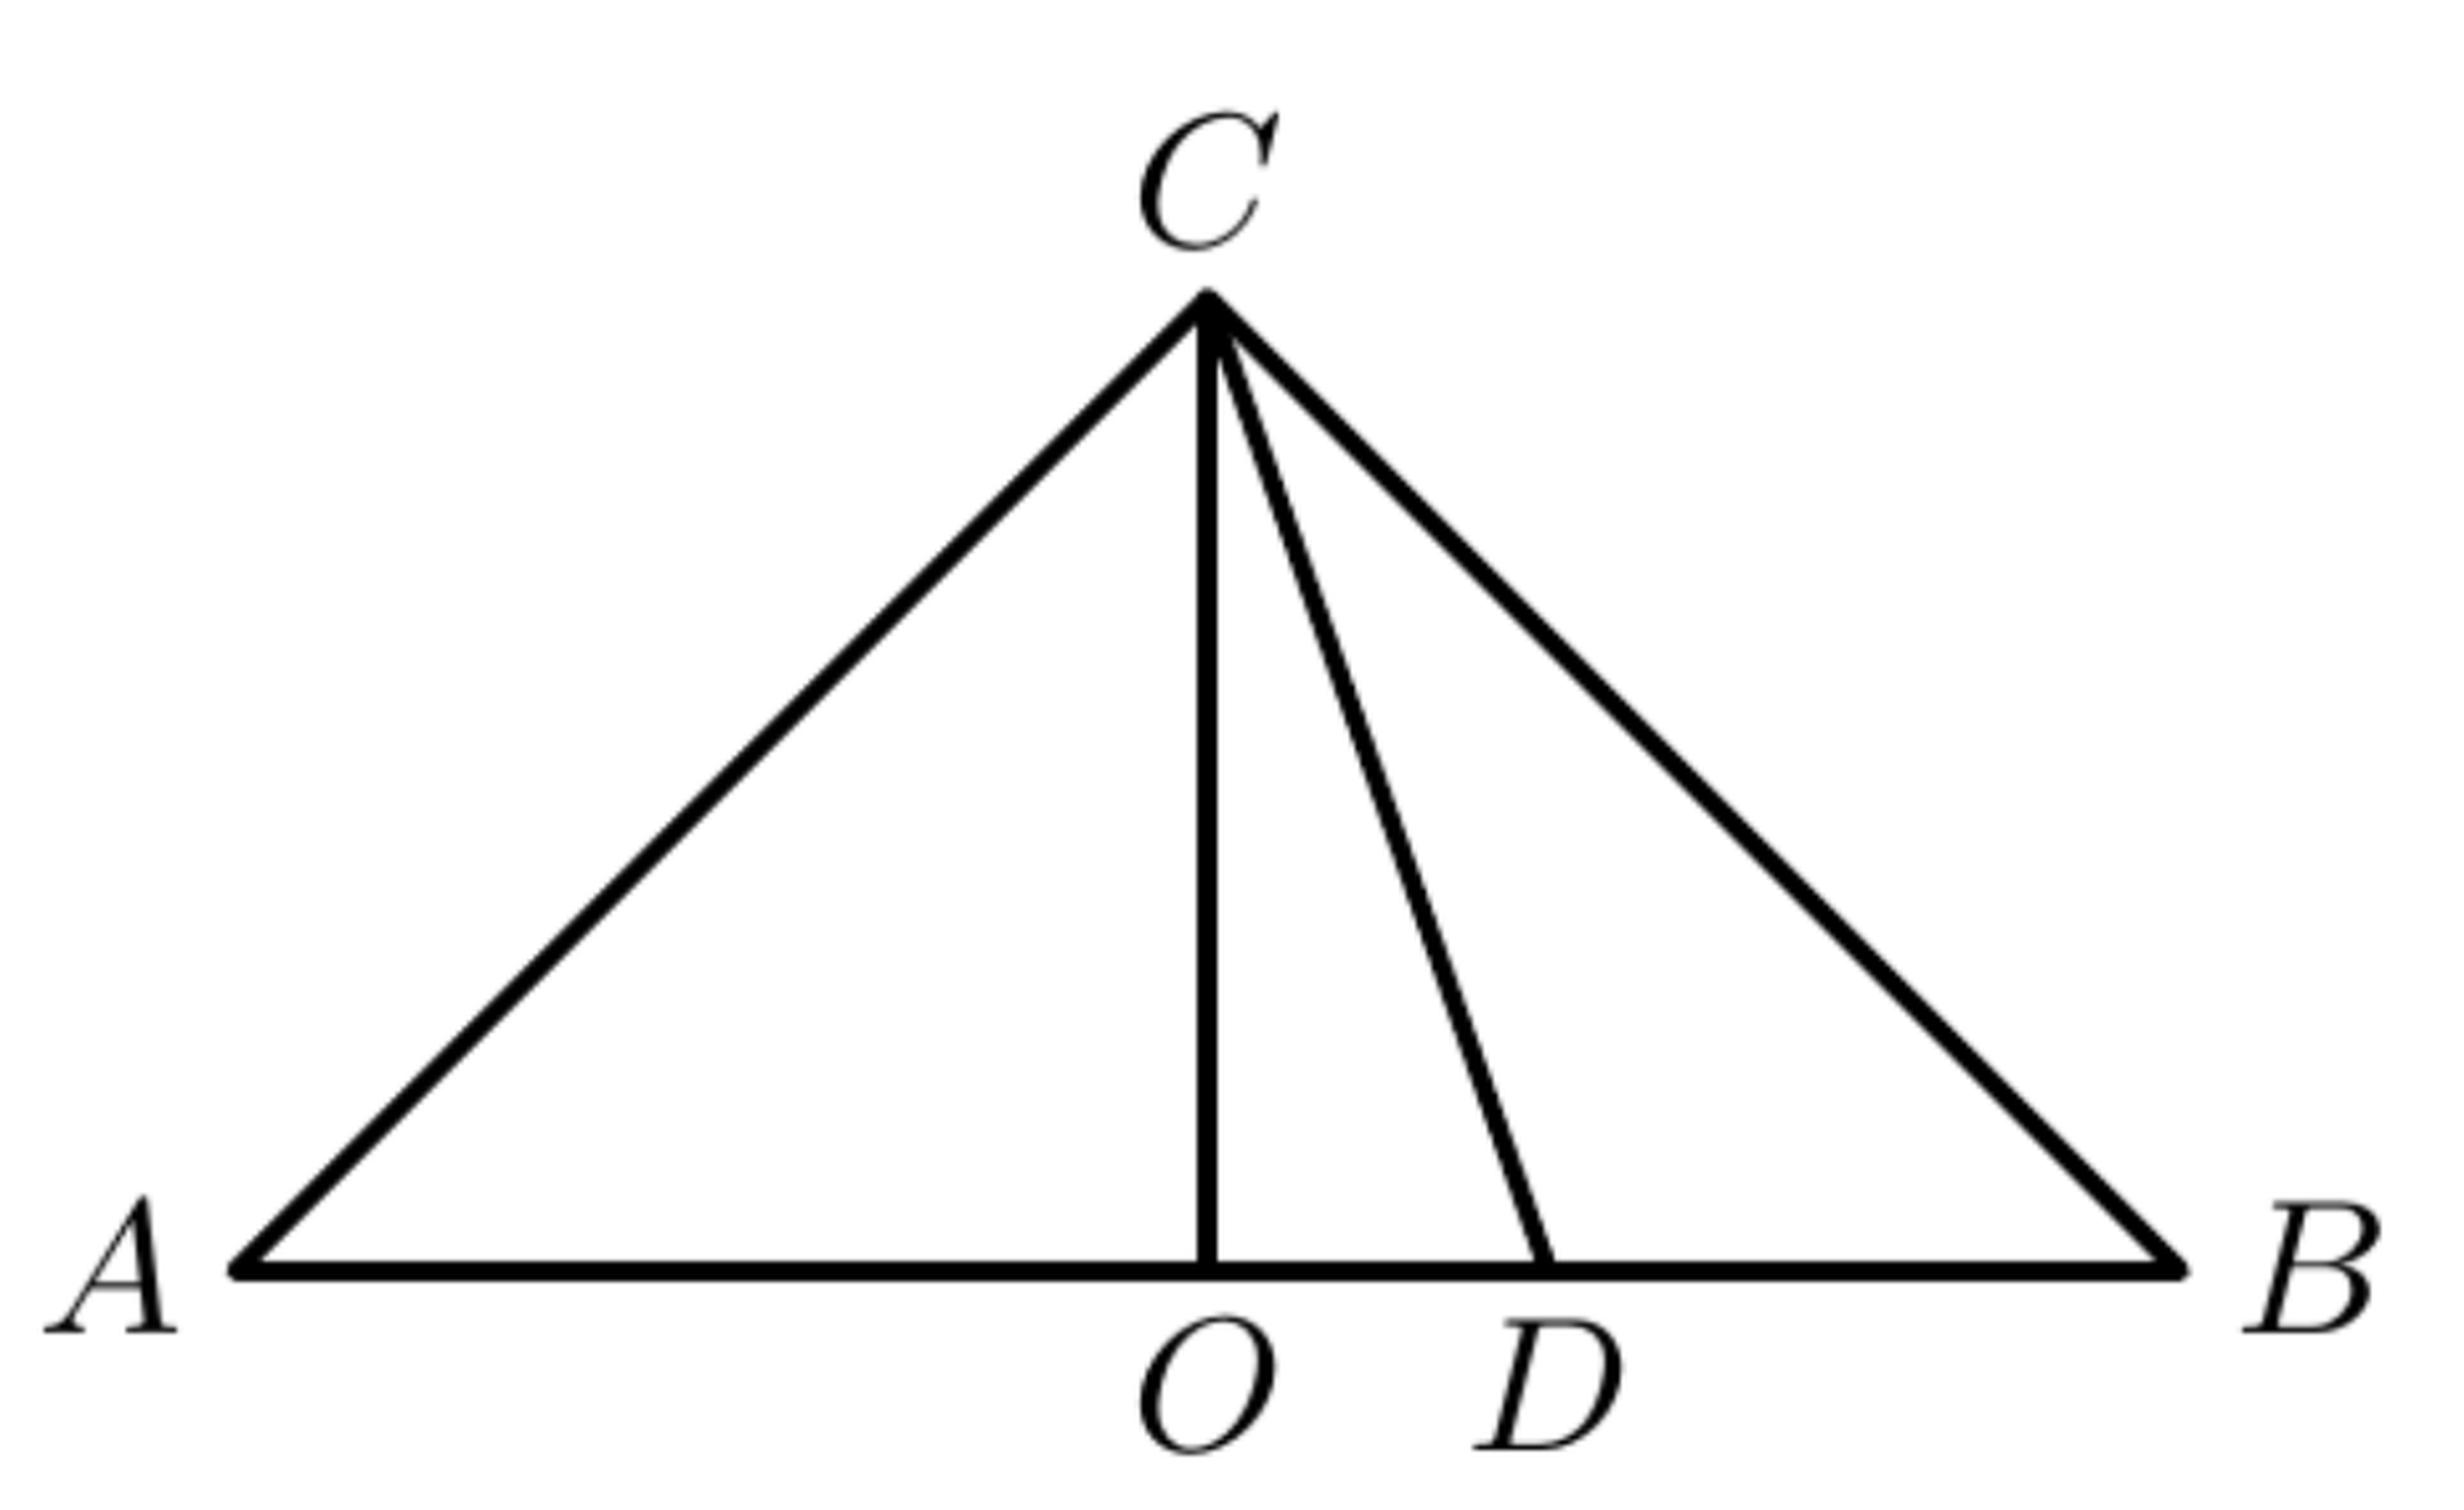
\includegraphics[width=0.34\textwidth]{figures/gao160_q16.png}
\end{center}

\keepwithprev
A. $\dfrac{a+b}{2}\geqslant\sqrt{ab}$ ($a>0,b>0$)\qquad B. $a^2+b^2\geqslant2\sqrt{ab}$ ($a>0,b>0$)

C. $\dfrac{a+b}{2}\leqslant\sqrt{\dfrac{a^2+b^2}{2}}$ ($a>0,b>0$)\qquad D. $\dfrac{2ab}{a+b}\leqslant\sqrt{ab}$ ($a>0,b>0$)

\ifanswer
\solbegin
\step{$CO=AO=\dfrac{a+b}{2},OD=\left\lvert a-\dfrac{a+b}{2}\right\rvert=\dfrac{\lvert a-b\rvert}{2}$，}
\step{$CD=\sqrt{CO^2+OD^2}=\sqrt{\dfrac{a^2+b^2}{2}}\geqslant CO=\dfrac{a+b}{2}$，}
\step{等号当且仅当 $a=b$ 时成立，故选 $C$.}
\solend
\fi

\end{enumerate}

\bigsec{三、解答题}

\begin{enumerate}
\setcounter{enumi}{16}

% === Q17 === cases 块算一行；判别式印等腰偏高三角 \Delta；解析 7 行
\item 已知幂函数 $f(x)=(m^2-2m-2)x^{m-1}$ 在 $(0,+\infty)$ 上是严格增函数.

(1) 求 $m$ 的值；

(2) 若关于 $x$ 的方程 $f(x)=(t+1)x-t^2$ 有两个不相等的正实根，求实数 $t$ 的取值范围.

\ifanswer
\solbegin
\step{(1) 幂函数的系数为 1，因此 $m^2-2m-2=1\Leftrightarrow(m-3)(m+1)=0$，}
\step{解得 $m=3$ 或 $m=-1$.}
\step{由 $f(x)$ 在 $(0,+\infty)$ 上严格递增，得 $m-1>0$，所以 $m=3$，}
\step{此时 $f(x)=x^2$.}
\step{(2) 原方程化为 $x^2-(t+1)x+t^2=0$，}
\step{方程有两个不相等的正实根，则 $\begin{cases}\Delta=(t+1)^2-4t^2=(1-t)(3t+1)>0\\t+1>0\\t^2>0\end{cases}$，}% 判别式原卷印等腰偏高三角 \Delta，照录
\step{得 $t\in\left(-\dfrac{1}{3},0\right)\cup(0,1)$.}
\solend
\fi

% === Q18 === 补集上划线 \overline{A}、\subseteq 带下划线、\varnothing；解析 8 行
\item 已知集合 $A=\{x\mid\lvert x-a\rvert<a-3\}$，$B=\left\{x\mid\dfrac{x+1}{x-2}\geqslant2\right\}$.

(1) 若 $a=5$，求 $\overline{A}\cap B$；

(2) 若 $A\cap B=A$，求实数 $a$ 的取值范围.

\ifanswer
\solbegin
\step{(1) $\dfrac{x+1}{x-2}\geqslant2\Leftrightarrow\dfrac{5-x}{x-2}\geqslant0\Leftrightarrow2<x\leqslant5,B=(2,5]$，}
\step{当 $a=5$ 时，$A=\{x\mid\lvert x-5\rvert<2\}=(3,7)$，于是 $\overline{A}=(-\infty,3]\cup[7,+\infty)$，}
\step{因此 $\overline{A}\cap B=(2,3]$.}
\step{(2) $A\cap B=A$ 等价于 $A\subseteq B$.}
\step{当 $a\leqslant3$ 时，$a-3\leqslant0$，$A=\varnothing$，满足条件.}
\step{当 $a>3$ 时，$\lvert x-a\rvert<a-3\Leftrightarrow3<x<2a-3,A=(3,2a-3)$，}
\step{此时 $A\subseteq B=(2,5]$ 等价于 $2a-3\leqslant5$，即 $a\leqslant4$，结合 $a>3$ 得 $3<a\leqslant4$.}
\step{合并两种情形，实数 $a$ 的取值范围为 $(-\infty,4]$.}
\solend
\fi

% === Q19 === 数据表 tabular 重排（高一130 成例）；cases 块算一行；解析 6 行
\item 作为我国最高水平的综合性运动会，全运会汇聚了国内顶尖体育健儿，某代表队从第 8 届全运会开始登上赛场，且参赛运动员人数逐年递增. 设 $t$ 为该代表队参赛后经过的届数，即第 8 届为 $t=0$，第 9 届为 $t=1$，以此类推. 经过 $t$ 届，运动员人数为 $y$ 人，具体数据如下：

\begin{center}
\begin{tabular}{cccccc}
$t$ & 0 & 1 & 2 & 3 & 4 \\
\hline
届数 & 8 & 9 & 10 & 11 & 12 \\
运动员人数（$y$ 人） & 4 & 11 & 25 & 53 & 109
\end{tabular}
\end{center}

(1) 现有以下两种函数模型：① $y=a\cdot b^t+c$ ($a>0,b>1$)；② $y=\log_a(t+b)+c$ ($b>0,a>1$). 请根据上表中运动员人数的增长规律，选出你认为符合的函数模型（不用说明理由），并利用表中前 3 组数据求出相应的函数解析式；

(2) 若参赛运动员人数按照 (1) 中求得的模型继续增长，在第几届全运会时，该代表队运动员人数将会首次超过 1000 人？

\ifanswer
\solbegin
\step{(1) 选模型①，将前 3 组数据代入，得 $\begin{cases}a+c=4\\ab+c=11\\ab^2+c=25\end{cases}$，}% 原卷印"选模型①"（圈数字①），OCR 误作"四"，照录①，见头注 ⑤ 3
\step{相邻两式相减，得 $a(b-1)=7$，$ab(b-1)=14$，}
\step{两式相除得 $b=2$，进而 $a=7$，$c=-3$，所求函数解析式为 $y=7\cdot2^t-3$.}
\step{(2) $y=7\cdot2^t-3$ 随 $t$ 的增大而增大，且 $t=7$ 时，$y=893<1000$；}
\step{$t=8$ 时，$y=1789>1000$，}
\step{$t$ 为非负整数，首次超过 1000 人时 $t=8$，对应第 $8+8=16$ 届全运会.}
\solend
\fi

% === Q20 === 解析 12 行（跨 08—09 页）
\item 已知函数 $f(x)=\log_a(a-a^x)$.

(1) 求该函数的定义域；

(2) 若 $a>1$，试判断关于 $x$ 的方程 $f(x)=2$ 是否有实数解，并说明理由；

(3) 若当 $x\in(-\infty,0]$ 时，关于 $x$ 的不等式 $f(x)\geqslant-1$ 恒成立，求实数 $a$ 的取值范围.

\ifanswer
\solbegin
\step{(1) 对数的底数须满足 $a>0$ 且 $a\ne1$，真数须满足 $a-a^x>0$，即 $a^x<a^1$.}% 原卷印 $a^1$，照录未化简，见头注 ⑤ 4
\step{当 $a>1$ 时，$x<1$，定义域为 $(-\infty,1)$.}
\step{当 $0<a<1$ 时，$x>1$，定义域为 $(1,+\infty)$.}
\step{(2) 当 $a>1$ 时，若 $f(x)=2$，则 $a-a^x=a^2\Rightarrow a^x=a(1-a)<0$，}
\step{这与 $a^x>0$ 矛盾，因此方程无实数解.}
\step{(3) 不等式在 $(-\infty,0]$ 上恒成立，须先保证该区间包含于函数的定义域，}
\step{由 (1) 得 $a>1$.}
\step{当 $x\leqslant0$ 时，$0<a^x\leqslant1$，所以 $a-a^x\geqslant a-1>0$.}
\step{由对数函数的单调性，$f(x)=\log_a(a-a^x)\geqslant\log_a(a-1)=f(0)$，}
\step{等号当且仅当 $x=0$ 时成立，}
\step{因此所求条件等价于 $\log_a(a-1)\geqslant-1\Leftrightarrow a-1\geqslant\dfrac{1}{a}\Leftrightarrow a^2-a-1\geqslant0$，}
\step{结合 $a>1$，得 $a\in\left[\dfrac{1+\sqrt{5}}{2},+\infty\right)$.}
\solend
\fi

% === Q21 === "和积平衡集"定义证明题；\N；解析 18 行（跨 09—10 页）
\item 已知有限集 $A=\{a_1,a_2,\cdots,a_n\}$ ($n\geqslant2,n\in\N$)，如果 $A$ 中元素 $a_i$ ($i=1,2,3,\cdots,n$) 满足 $a_1+a_2+a_3+\cdots+a_n=a_1\times a_2\times\cdots\times a_n$，就称 $A$ 为“和积平衡集”.

(1) 分别判断集合 $A=\{1,2,3,4\}$，$B=\{4+2\sqrt{2},4-2\sqrt{2}\}$ 是否为“和积平衡集”；

(2) 已知 $a_1$、$a_2$ 是两个不同的正数，且 $\{a_1,a_2\}$ 是“和积平衡集”，请用反证法证明：$a_1$、$a_2$ 至少有一个大于 2；

(3) 若 $a_i\geqslant1$，且 $a_i\in\N$，求所有符合条件的“和积平衡集”.

\ifanswer
\solbegin
\step{(1) 因为 $1+2+3+4=10\ne24=1\times2\times3\times4$，所以 $A$ 不是“和积平衡集”.}
\step{因为 $(4+2\sqrt{2})+(4-2\sqrt{2})=8=(4+2\sqrt{2})(4-2\sqrt{2})$，}
\step{所以 $B$ 是“和积平衡集”.}
\step{(2) 假设 $a_1$、$a_2$ 都不大于 2，则 $\dfrac{1}{a_1}\geqslant\dfrac{1}{2},\dfrac{1}{a_2}\geqslant\dfrac{1}{2}$，}
\step{由于 $a_1\ne a_2$，上述两个不等式至少有一个严格成立.}
\step{而 $a_1+a_2=a_1a_2$，两边除以 $a_1a_2>0$，得 $1=\dfrac{1}{a_1}+\dfrac{1}{a_2}>\dfrac{1}{2}+\dfrac{1}{2}=1$，矛盾，}
\step{所以 $a_1$、$a_2$ 至少有一个大于 2.}
\step{(3) 不妨设 $a_1<a_2<\cdots<a_n$，由各元素均为正整数，得 $a_i\geqslant i$.}
\step{若 $n\geqslant4$，因其余因子均不小于 1，}
\step{有 $a_1a_2\cdots a_n\geqslant a_2a_{n-1}a_n\geqslant2(n-1)a_n>na_n>a_1+a_2+\cdots+a_n$，}
\step{与和积平衡条件矛盾，因此只需讨论 $n=2,3$.}
\step{当 $n=2$ 时，$a_1+a_2=a_1a_2\Leftrightarrow(a_1-1)(a_2-1)=1$，}
\step{两个因子均为非负整数，只能有 $a_1=a_2=2$，与元素互不相同矛盾.}
\step{当 $n=3$ 时，若 $a_1\geqslant2$，则 $a_2\geqslant3$，从而 $a_1a_2a_3\geqslant6a_3>3a_3>a_1+a_2+a_3$，}
\step{矛盾，因此 $a_1=1$.}
\step{此时 $1+a_2+a_3=a_2a_3\Leftrightarrow(a_2-1)(a_3-1)=2$，}
\step{由 $1\leqslant a_2-1<a_3-1$，得 $a_2-1=1$、$a_3-1=2$，即 $a_2=2$、$a_3=3$.}
\step{检验 $1+2+3=1\times2\times3=6$，所求集合为 $\{1,2,3\}$.}
\solend
\fi

\end{enumerate}

\end{document}
